% !TEX program = xelatex

\documentclass[11pt, a4paper, twoside]{book}

% ==============================================================================
% 1. HỖ TRỢ TIẾNG VIỆT VÀ FONT CHỮ
% ==============================================================================
\usepackage{fontspec}

\setmainfont{Times New Roman}       % font chữ chính (serif)
\setsansfont{Arial}                 % font không chân (sans-serif)
\setmonofont{Courier New}           % font mono (code, terminal)

% Gói hỗ trợ tiếng Việt
\usepackage[vietnamese]{babel}


% ==============================================================================
% 2. CÁC GÓI TOÁN HỌC VÀ KHOA HỌC
% ==============================================================================
\usepackage{amsmath, amssymb, amsfonts, amsthm, caption, tabularx, csquotes}

% ==============================================================================
% 3. BỐ CỤC VÀ ĐỊNH DẠNG TRANG
% ==============================================================================
\usepackage[
    a4paper,
    top=2.5cm,
    bottom=2.5cm,
    left=3cm,
    right=2.5cm,
    headsep=1cm,
    footskip=1cm,
    twoside
]{geometry}
\usepackage{enumitem}
\setlist{nosep}
\usepackage{graphicx}
\graphicspath{{images/}} 
\usepackage[dvipsnames]{xcolor} 
\usepackage{hyperref}
\hypersetup{
    colorlinks=true,
    linkcolor=MidnightBlue,
    filecolor=magenta,      
    urlcolor=RoyalBlue,
    citecolor=ForestGreen,
    pdftitle={Giáo trình NLP Toàn tập},
    pdfauthor={Tên tác giả},
}
\usepackage{booktabs}
% ==============================================================================
% 4. TÙY BIẾN TIÊU ĐỀ
% ==============================================================================
\usepackage{fancyhdr}
\pagestyle{fancy}
\fancyhf{}
\fancyhead[L]{\leftmark}
\fancyfoot[C]{Công Thái Học (ngu)}
\usepackage{titlesec}
\titleformat{\part}[display]
  {\normalfont\Huge\bfseries\centering}
  {\partname~\thepart}
  {20pt}
  {\Huge}
\titlespacing*{\part}{0pt}{50pt}{40pt}

\titleformat{\chapter}[display]
  {\normalfont\huge\bfseries}
  {\chaptertitlename~\thechapter}
  {20pt}
  {\huge\bfseries}
\titlespacing*{\chapter}{0pt}{40pt}{30pt}

\titleformat{\section}
  {\normalfont\Large\bfseries\color{MidnightBlue}}
  {\thesection.}
  {1em}
  {}
\titleformat{\subsection}
  {\normalfont\large\bfseries\color{OliveGreen}}
  {\thesubsection.}
  {1em}
  {}
\titleformat{\subsubsection}
  {\normalfont\normalsize\bfseries\color{Brown}}
  {\thesubsubsection.}
  {1em}
  {}

% ==============================================================================
% 5. CODE & BOX
% ==============================================================================
\usepackage{minted}
\setminted{
    frame=lines,
    framesep=2mm,
    numbersep=0pt
    baselinestretch=1.2,
    fontsize=\small,
    linenos,
    breaklines,
    breakanywhere
}
\usepackage[most]{tcolorbox}
\tcbuselibrary{skins}

\newtcbtheorem{definition}{Định nghĩa}{
    colback=blue!5!white,
    colframe=blue!75!black,
    fonttitle=\bfseries,
    breakable
}{def}
\newtcbtheorem{example}{Ví dụ}{
    colback=green!5!white,
    colframe=green!50!black,
    fonttitle=\bfseries,
    before skip=0.5em,   
    after skip=0.5em,   
    boxsep=1mm,          
    breakable
}{ex}
\newtcbtheorem[
    auto counter, 
    number within=chapter,
    list inside=rcp
]{recipe}{Recipe \thetcbcounter}{
    colback=orange!5!white,
    colframe=orange!75!black,
    fonttitle=\bfseries,
    title={Recipe \thechapter.\arabic{tcbcounter}:}
}{rcp}

% ==============================================================================
% 6. LỆNH PHỤ
% ==============================================================================
\newcommand{\newtag}{\textcolor{red}{\textnormal{\bfseries\small [MỚI & SỬA ĐỔI]}}}
\newcommand{\reftag}{\textcolor{blue}{\textnormal{\bfseries\small [THAM KHẢO]}}}

% ==============================================================================
% 7. THÔNG TIN SÁCH
% ==============================================================================
\title{GIÁO TRÌNH NLP TOÀN TẬP \\ \large}
\author{Đinh Công Thái}
\date{\today}

%%%%%%%%%%%%%%%%%%%%%%%%%%%%%%%%%%%%%%%%%%%%%%%%%%%%%%%%%%%%%%%%%%%%%%%%%%%%%%%%
\begin{document}

\maketitle
\tableofcontents

\mainmatter

\chapter*{Lời nói đầu}
\addcontentsline{toc}{chapter}{Lời nói đầu} 
\markboth{Lời nói đầu}{} 

\noindent
Xin chào, mình là \textbf{Đinh Công Thái}, sinh viên lớp IT1-K67, ngành Khoa học Máy tính, Trường Đại học Bách khoa Hà Nội. Là nghiên cứu sinh tại Viên Nghiên cứu và Ứng dụng Trí tuệ nhân tạo của \textbf{PGS.TS Nguyễn Phi Lê}, đồng thời nghiên cứu và làm việc dưới sự hướng dẫn của anh \textbf{Nguyễn Tuấn Dũng}.\\


\vspace{1em}
\noindent
\textbf{Vậy cuốn giáo trình này ra đời để làm gì?}  

Mình viết nó cho những bạn đang mơ hồ, không định hướng, không biết AI bắt đầu từ đâu, nhưng có chút tò mò và muốn thử. Nội dung tập trung vào \textbf{Xử lý ngôn ngữ tự nhiên (NLP)}

Sách này không hứa biến bạn thành chuyên gia sau một đêm. Nhưng nó sẽ là một bản đồ để bạn không bị lạc trôi quá lâu, và nếu thấy hứng thú thì có thể đi xa hơn, sớm hơn.


Cách làm của mình khá ra tác phẩm này có thể tóm tắt như sau:

\begin{itemize}
    \item \textbf{Soạn mục lục} $\rightarrow$ dựng cái khung nhà cho con chatbot.
    \item \textbf{Tìm \& gom paper/tài liệu}, để LLM không bịa, đồng thời cũng để cho kiến thức được sâu sắc và bám sát.
    \item \textbf{Chia thư mục theo từng phần/tiểu mục} $\rightarrow$ giữ cấu trúc rõ ràng.
    \item \textbf{Soạn rule} $\rightarrow$ chính là \textit{style guide}: văn phong, yêu cầu ví dụ, công thức, hình minh hoạ…
    \item \textbf{Tool 1 (lưu context)} $\rightarrow$ giúp LLM nhớ liền mạch, không quên mình vừa viết gì ở trang trước.
    \item \textbf{Tool 2 (API xuất bản)} $\rightarrow$ gửi query theo từng mục và nhận lại nội dung thành file tương ứng.
    \item \textbf{Tool 3 (tự động review \& bổ sung)} $\rightarrow$ LLM đọc lại chính nội dung đã sinh, so với rule + nguồn, rồi nhận xét/gợi ý sửa.
\end{itemize}

Kết quả cuối cùng: phần kiến thức cốt lõi thì mình đã kiểm tra lại cẩn thận. 
Còn nếu  có vài chỗ đọc hơi lạ lạ thì có thể đó là \textit{hallucination}.


\vspace{1em}
\noindent
\textbf{Cấu trúc cuốn sách}  

\begin{itemize}[leftmargin=*]
    \item \textbf{Phần 1: Lý thuyết NLP} – kể câu chuyện từ những nền tảng cơ bản cho tới các mô hình hiện đại như Transformer. Đọc phần này để biết “tại sao lại như vậy”.  
    \item \textbf{Phần 2: Thực chiến NLP} – biến lý thuyết thành code, dự án, ứng dụng. Đọc phần này để biết “làm thế nào”.  
\end{itemize}

Hai phần này bổ sung cho nhau. Biết lý thuyết mà không thực hành thì dễ nói cho vui. Còn chỉ thực hành mà không hiểu gốc thì cũng dễ trở thành copy-paste developer.  

\begin{flushright}
\textit{Trân trọng,} \\[0.5em]
Đinh Công Thái
\end{flushright}

\part{BÁCH KHOA TOÀN THƯ VỀ LÝ THUYẾT NLP}

\textit{Chào mừng bạn đến với nền tảng lý thuyết của Xử lý Ngôn ngữ Tự nhiên. Mục tiêu của Phần 1 là cung cấp một cái nhìn toàn diện, sâu sắc và có hệ thống về TẤT CẢ các khái niệm, kiến trúc và thuật toán lý thuyết đã định hình nên ngành NLP. Chúng ta sẽ bắt đầu từ những nguyên lý ngôn ngữ học cơ bản, đi qua kỷ nguyên thống kê, khám phá các kiến trúc mạng nơ-ron kinh điển, và cuối cùng là làm chủ kiến trúc Transformer - nền tảng của các mô hình ngôn ngữ lớn hiện đại. Mỗi chương là một khối kiến thức độc lập nhưng có sự kết nối chặt chẽ, cùng nhau xây dựng nên một nền tảng vững chắc để bạn có thể hiểu "tại sao" và "như thế nào" các công nghệ NLP hoạt động. Hãy bắt đầu hành trình khám phá này.}

% \chapter{CÁC KIẾN TRÚC MẠNG NƠ-RON KINH ĐIỂN}
\label{chap:deep_learning_architectures}

Chào mừng bạn đến với kỷ nguyên học sâu của NLP. Trong chương 2, chúng ta đã thấy các mô hình thống kê như N-gram có thể nắm bắt các phụ thuộc cục bộ, nhưng lại bất lực trước các mối quan hệ tầm xa. Cuộc cách mạng word embedding đã cho chúng ta các vector từ mang đầy ngữ nghĩa, nhưng làm thế nào để kết hợp chúng lại nhằm hiểu được ý nghĩa của cả một câu hay một đoạn văn?

Chương này sẽ giới thiệu các kiến trúc mạng nơ-ron nền tảng được thiết kế đặc biệt để xử lý dữ liệu dạng chuỗi như ngôn ngữ tự nhiên. Những kiến trúc này không chỉ đơn thuần "nhìn" vào các từ một cách riêng lẻ, mà còn có khả năng "ghi nhớ" và "lý luận" dựa trên thông tin đã xử lý trước đó, cho phép chúng nắm bắt được ngữ cảnh và các phụ thuộc phức tạp trong câu.
% % !TEX root = ../../main.tex 
% File: part2/chapters1/chap1_1.tex


\section{Phác thảo Quy trình Dự án NLP Tinh gọn}
\label{sec:nlp_project_workflow}

Chào mừng bạn đến với phần thực chiến của giáo trình. Trước khi chúng ta lao vào việc viết code và huấn luyện các mô hình phức tạp, điều quan trọng nhất là phải có một "tấm bản đồ" -- một quy trình làm việc có hệ thống để dẫn dắt dự án từ một ý tưởng mơ hồ đến một sản phẩm hữu ích.

Việc thiếu một quy trình rõ ràng là một trong những nguyên nhân hàng đầu khiến các dự án học máy thất bại. Các đội nhóm có thể tốn hàng tháng trời để xây dựng một mô hình phức tạp chỉ để nhận ra rằng nó không giải quyết đúng bài toán kinh doanh, hoặc dữ liệu không đủ chất lượng.

Quy trình dưới đây được thiết kế theo một vòng lặp tinh gọn, nhấn mạnh vào việc tạo ra giá trị nhanh chóng, thu thập phản hồi, và lặp lại. Nó không phải là một thác nước cứng nhắc, mà là một chu trình linh hoạt.

\begin{center}
    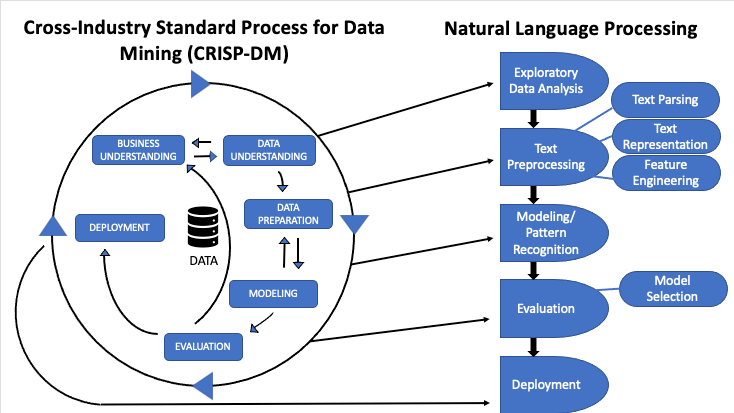
\includegraphics[width=1.0\textwidth]{nlp_workflow_cycle.png}
    \captionof{figure}{Quy trình Dự án NLP Tinh gọn: Một chu trình lặp đi lặp lại từ việc xác định bài toán đến triển khai và giám sát.}
    \label{fig:nlp_workflow_cycle}
\end{center}

\subsection{Vòng lặp 0: Xác định Bài toán và Thiết lập Đường cơ sở (Baseline)}
\label{ssec:workflow_step0}
Đây là bước quan trọng nhất, quyết định sự thành bại của toàn bộ dự án.

\subsubsection{1. Hiểu rõ Mục tiêu (Problem Framing)}
\begin{itemize}
    \item \textbf{Câu hỏi cần trả lời:} Chúng ta đang cố gắng giải quyết vấn đề kinh doanh/nghiên cứu nào? Tác động mong muốn là gì? (Ví dụ: "giảm 30\% thời gian phản hồi của nhân viên hỗ trợ", "tự động phân loại 80\% tin tức đầu vào").
    \item \textbf{Xác định Input và Output:} Đầu vào của mô hình là gì (văn bản thô, bình luận, email)? Đầu ra mong muốn là gì (một nhãn, một đoạn văn bản tóm tắt, một câu trả lời)?
    \item \textbf{Định hình bài toán NLP:} Ánh xạ vấn đề kinh doanh thành một bài toán NLP cụ thể. Ví dụ: "Giảm thời gian phản hồi" $\rightarrow$ "Xây dựng mô hình phân loại email để tự động định tuyến đến đúng phòng ban".
\end{itemize}

\subsubsection{2. Định nghĩa Metric Thành công}
\begin{itemize}
    \item \textbf{Metric Máy học (Offline):} Chọn các metric kỹ thuật để đánh giá mô hình trong quá trình phát triển (ví dụ: F1-score, Accuracy, BLEU). Metric này phải phản ánh được mục tiêu kinh doanh.
    \item \textbf{Metric Kinh doanh (Online):} Xác định cách bạn sẽ đo lường tác động thực tế của mô hình sau khi triển khai (ví dụ: tỷ lệ click, thời gian giải quyết ticket, mức độ hài lòng của khách hàng).
\end{itemize}

\subsubsection{3. Thiết lập một Đường cơ sở (Baseline) Đơn giản}
\begin{tcolorbox}[
    title=Lời khuyên quan trọng: Bắt đầu một cách "ngu ngốc",
    colback=yellow!10!white, colframe=yellow!50!black, fonttitle=\bfseries
]
Đừng bao giờ bắt đầu một dự án bằng việc xây dựng một mô hình Transformer phức tạp. Hãy bắt đầu với giải pháp đơn giản nhất có thể. Một baseline tốt không chỉ cho bạn một điểm để so sánh, mà còn có thể đủ tốt để giải quyết 80\% vấn đề với 20\% công sức.
\end{tcolorbox}
\begin{itemize}
    \item \textbf{Các ý tưởng cho Baseline:}
        \begin{itemize}
            \item \textbf{Không dùng ML:} Một hệ thống dựa trên từ khóa hoặc biểu thức chính quy (regex).
            \item \textbf{Mô hình Thống kê kinh điển:} Sử dụng `TF-IDF` kết hợp với `Logistic Regression` hoặc `Naive Bayes`. Các thư viện như `Scikit-learn` giúp việc này trở nên cực kỳ nhanh chóng.
            \item \textbf{Mô hình Zero-shot:} Sử dụng API của một LLM lớn (như GPT-4) với một prompt zero-shot. Đây là một baseline rất mạnh mẽ trong kỷ nguyên hiện đại.
        \end{itemize}
\end{itemize}

Baseline này sẽ là thước đo để bạn biết liệu những nỗ lực phức tạp hơn của mình có thực sự mang lại giá trị hay không.

\subsection{Vòng lặp 1: Phát triển Mô hình (Model Development)}
\label{ssec:workflow_step1}
Đây là vòng lặp cốt lõi của việc xây dựng và cải tiến mô hình.

\subsubsection{4. Thu thập và Chuẩn bị Dữ liệu}
Đây thường là phần tốn nhiều thời gian nhất.
\begin{itemize}
    \item \textbf{Thu thập (Collection):} Lấy dữ liệu từ các nguồn (cơ sở dữ liệu, API, web scraping).
    \item \textbf{Làm sạch (Cleaning):} Xử lý các vấn đề như mã hóa ký tự, loại bỏ các thẻ HTML, chuẩn hóa văn bản.
    \item \textbf{Gán nhãn (Labeling):} Nếu là bài toán có giám sát, đây là bước cực kỳ quan trọng. Sử dụng các công cụ như `Label Studio` hoặc các kỹ thuật gán nhãn yếu (weak supervision).
    \item \textbf{Phân chia Dữ liệu (Splitting):} Chia dữ liệu thành các tập Huấn luyện (Train), Đánh giá (Validation/Dev), và Kiểm tra (Test). \textbf{Không bao giờ} được "nhìn" vào tập Test trong quá trình phát triển.
\end{itemize}

\subsubsection{5. Huấn luyện Mô hình}
\begin{itemize}
    \item \textbf{Lựa chọn Mô hình:} Dựa trên baseline và yêu cầu của bài toán, chọn một kiến trúc phù hợp (ví dụ: một mô hình từ Hugging Face Hub).
    \item \textbf{Huấn luyện/Fine-tuning:} Thực hiện quá trình huấn luyện.
    \item \textbf{Theo dõi Thí nghiệm (Experiment Tracking):} Sử dụng các công cụ như `Weights \& Biases` hoặc `MLflow` để ghi lại mọi thứ: phiên bản code, siêu tham số, metric, và các mô hình đã được huấn luyện. Việc này là tối quan trọng để đảm bảo tính tái lập (reproducibility) và so sánh các thử nghiệm.
\end{itemize}

\subsubsection{6. Phân tích Lỗi (Error Analysis)}
Đây là bước mà nhiều người bỏ qua, nhưng nó lại là chìa khóa để cải tiến mô hình một cách thông minh.
\begin{itemize}
    \item \textbf{Mục tiêu:} Không chỉ nhìn vào con số metric tổng thể (ví dụ: F1 = 85\%), mà phải hiểu \textbf{tại sao} mô hình lại sai ở 15\% còn lại.
    \item \textbf{Quy trình:}
        \begin{enumerate}
            \item Lấy một mẫu các dự đoán sai trên tập validation.
            \item Phân loại các lỗi này thành các nhóm. Ví dụ: "mô hình sai ở các câu bị phủ định", "mô hình nhầm lẫn giữa hai lớp A và B", "lỗi do dữ liệu gán nhãn sai".
            \item \textbf{Ưu tiên:} Tập trung nỗ lực vào việc giải quyết nhóm lỗi lớn nhất và có tác động nhất. Ví dụ, nếu mô hình thường sai ở các câu phủ định, bạn có thể cần thu thập thêm dữ liệu về loại câu này hoặc sử dụng kỹ thuật tăng cường dữ liệu.
        \end{enumerate}
\end{itemize}
Vòng lặp (Huấn luyện $\rightarrow$ Phân tích lỗi $\rightarrow$ Cải thiện dữ liệu/mô hình) được lặp lại cho đến khi mô hình đạt được hiệu năng mong muốn trên tập validation.

\subsection{Vòng lặp 2: Triển khai và Giám sát (Deployment \& Monitoring)}
\label{ssec:workflow_step2}
Một mô hình chỉ thực sự tạo ra giá trị khi nó được đưa vào sử dụng.

\subsubsection{7. Đóng gói và Triển khai (Deployment)}
\begin{itemize}
    \item \textbf{Tối ưu hóa:} Áp dụng các kỹ thuật như lượng tử hóa (quantization) hoặc chưng cất (distillation) để làm cho mô hình nhỏ hơn và nhanh hơn.
    \item \textbf{Đóng gói (Packaging):} Đóng gói mô hình và các thành phần phụ thuộc của nó vào một định dạng có thể triển khai, ví dụ như một container Docker.
    \item \textbf{Phục vụ (Serving):} Triển khai mô hình như một API endpoint (sử dụng các framework như `FastAPI` hoặc `BentoML`) để các ứng dụng khác có thể gọi đến.
\end{itemize}

\subsubsection{8. Giám sát và Bảo trì (Monitoring \& Maintenance)}
Công việc không kết thúc sau khi triển khai.
\begin{itemize}
    \item \textbf{Giám sát Hiệu năng:} Theo dõi các metric của mô hình trong môi trường thực tế.
    \item \textbf{Phát hiện Trôi dạt Dữ liệu (Data Drift):} Thế giới thực luôn thay đổi. Cách người dùng viết và các chủ đề họ quan tâm có thể thay đổi theo thời gian. Cần có cơ chế để phát hiện khi nào phân phối dữ liệu đầu vào thực tế bắt đầu khác biệt so với dữ liệu huấn luyện.
    \item \textbf{Thu thập Phản hồi và Huấn luyện lại:} Thiết lập một vòng lặp để thu thập các dự đoán sai từ môi trường production, gán nhãn lại chúng, và sử dụng chúng để định kỳ huấn luyện lại (re-train) mô hình afin d'améliorer sa performance au fil du temps.
\end{itemize}
Quy trình tinh gọn này đảm bảo rằng bạn luôn tập trung vào việc tạo ra giá trị, học hỏi từ dữ liệu và các lỗi sai, và xây dựng các hệ thống NLP mạnh mẽ và bền vững.
% % File: chapters_part1/chap1_linguistics.tex

\section{Nền tảng Ngôn ngữ học cho NLP}
\label{sec:nen_tang_ngon_ngu_hoc}

Trong kỷ nguyên của Học sâu, khi các mô hình Transformer khổng lồ dường như có thể "học" mọi thứ từ dữ liệu thô, một câu hỏi chính đáng được đặt ra: "Liệu kiến thức về Ngôn ngữ học có còn cần thiết?". Câu trả lời là một tiếng "Có" dứt khoát.

Mặc dù chúng ta không còn phải viết tay các bộ quy tắc ngữ pháp phức tạp, việc hiểu các cấu trúc và nguyên lý cơ bản của ngôn ngữ mang lại những lợi ích to lớn:
\begin{itemize}
    \item \textbf{Thiết kế tác vụ (Task Design):} Giúp chúng ta định hình các bài toán NLP một cách có ý nghĩa. Ví dụ, tại sao "Nhận dạng Thực thể Tên" (NER) lại là một bài toán quan trọng? Vì "thực thể" là một khái niệm ngữ nghĩa cơ bản.
    \item \textbf{Kỹ thuật đặc trưng (Feature Engineering):} Cung cấp ý tưởng cho các đặc trưng hữu ích, đặc biệt khi dữ liệu bị hạn chế.
    \item \textbf{Phân tích lỗi (Error Analysis):} Giúp chúng ta hiểu tại sao một mô hình thất bại. Liệu nó thất bại vì không hiểu được cấu trúc cú pháp phức tạp, hay vì không giải quyết được sự đa nghĩa của từ?
    \item \textbf{Đánh giá (Evaluation):} Giúp xây dựng các bộ dữ liệu đánh giá có thể kiểm tra các năng lực ngôn ngữ cụ thể của mô hình.
\end{itemize}

Mục này sẽ giới thiệu những khái niệm Ngôn ngữ học cốt lõi nhất, đóng vai trò là lăng kính để chúng ta nhìn vào các bài toán NLP trong suốt giáo trình này.

\subsection{Các cấp độ phân tích ngôn ngữ: Hình thái học, Cú pháp, Ngữ nghĩa, Ngữ dụng}
\label{ssec:cap_do_phan_tich}

Ngôn ngữ học thường phân tích ngôn ngữ theo một hệ thống các cấp độ, đi từ đơn vị nhỏ nhất đến ý nghĩa trong bối cảnh rộng lớn nhất. Đây là một khung khái niệm vô cùng hữu ích để phân loại các bài toán NLP.

\paragraph{1. Hình thái học (Morphology)}
Là nghiên cứu về cấu trúc bên trong của từ. Hình thái học xem xét cách các từ được tạo thành từ những đơn vị có nghĩa nhỏ hơn gọi là \textbf{hình vị (morphemes)}.
\begin{itemize}
    \item \textbf{Ví dụ (tiếng Anh):} Từ \textit{unhappiness} được cấu tạo từ 3 hình vị: tiền tố \textit{un-} (phủ định), gốc từ \textit{happi} (hạnh phúc), và hậu tố \textit{-ness} (danh từ hóa).
    \item \textbf{Ví dụ (tiếng Việt):} Tiếng Việt là một ngôn ngữ đơn lập (isolating language), nên cấu trúc hình thái không phức tạp như tiếng Anh. Tuy nhiên, khái niệm này vẫn có thể áp dụng cho các từ ghép như \textit{học sinh} (gồm hình vị \textit{học} và \textit{sinh}) hay \textit{nhà khoa học} (\textit{nhà-} + \textit{khoa học}).
    \item \textbf{Ứng dụng trong NLP:} Lemmatization (đưa từ về dạng gốc, ví dụ: "running" $\rightarrow$ "run"), Stemming (cắt bỏ hậu tố), Phân tích hình thái.
\end{itemize}

\paragraph{2. Cú pháp (Syntax)}
Là nghiên cứu về cách các từ kết hợp với nhau để tạo thành các cụm từ (phrases) và câu (sentences) đúng ngữ pháp. Cú pháp tập trung vào \textbf{quy tắc cấu trúc} của câu.
\begin{itemize}
    \item \textbf{Ví dụ:} Câu "Con mèo đuổi con chuột" là đúng cú pháp tiếng Việt. Câu *"Mèo con chuột con đuổi"* thì không, mặc dù các từ vẫn giữ nguyên. Cú pháp quy định trật tự từ và các mối quan hệ ngữ pháp.
    \item \textbf{Ứng dụng trong NLP:} Phân tích cú pháp (Parsing), Gán nhãn Từ loại (Part-of-Speech Tagging), Kiểm tra ngữ pháp (Grammar Checking).
\end{itemize}

\paragraph{3. Ngữ nghĩa (Semantics)}
Là nghiên cứu về \textbf{ý nghĩa} của từ, cụm từ và câu, độc lập với ngữ cảnh. Ngữ nghĩa trả lời câu hỏi "Câu này có nghĩa là gì?".
\begin{itemize}
    \item \textbf{Ví dụ:} Câu "Colorless green ideas sleep furiously" (Những ý tưởng xanh không màu ngủ một cách giận dữ) của Noam Chomsky là một câu đúng về mặt cú pháp nhưng vô nghĩa về mặt ngữ nghĩa.
    \item Thử thách lớn của ngữ nghĩa là \textbf{sự mơ hồ (ambiguity)}. Ví dụ, từ "đường" có thể là "con đường" hoặc "đường ăn". Câu "Tôi thấy người đàn ông trên ngọn đồi với chiếc kính thiên văn" có thể có nghĩa là tôi dùng kính để thấy anh ta, hoặc anh ta là người có chiếc kính.
    \item \textbf{Ứng dụng trong NLP:} Phân biệt ý của từ (Word Sense Disambiguation - WSD), Gán nhãn vai nghĩa (Semantic Role Labeling - SRL), Biểu diễn ý nghĩa câu.
\end{itemize}

\paragraph{4. Ngữ dụng (Pragmatics)}
Là nghiên cứu về cách ngữ cảnh ảnh hưởng đến việc diễn giải ý nghĩa. Ngữ dụng xem xét ý định của người nói và cách người nghe hiểu được ý định đó. Nó trả lời câu hỏi "Người nói \textbf{muốn} nói gì khi nói câu này?".
\begin{itemize}
    \item \textbf{Ví dụ:} Nếu ai đó nói "Ở đây nóng quá", về mặt ngữ nghĩa, đó là một câu trần thuật về nhiệt độ. Nhưng về mặt ngữ dụng, đó có thể là một lời yêu cầu "Làm ơn bật quạt/điều hòa lên".
    \item \textbf{Ứng dụng trong NLP:} Phân tích hội thoại (Discourse Analysis), Phân giải đồng tham chiếu (Coreference Resolution - xác định "anh ấy" trong một câu là đang chỉ đến ai), Nhận dạng hành động nói (Speech Act Recognition), các hệ thống đối thoại (Dialogue Systems).
\end{itemize}

Bốn cấp độ này tạo thành một chuỗi xử lý tự nhiên: từ nhận diện các đơn vị nhỏ nhất của từ (hình thái), đến cách chúng kết hợp thành câu (cú pháp), rồi ý nghĩa của câu đó (ngữ nghĩa), và cuối cùng là ý nghĩa trong một bối cảnh cụ thể (ngữ dụng).

\subsection{Ngữ pháp hình thức (Formal Grammars): Ngữ pháp phi ngữ cảnh (CFG)}
\label{ssec:cfg}

Để máy tính có thể "hiểu" được cú pháp, các nhà ngôn ngữ học và khoa học máy tính đã phát triển các hệ thống quy tắc toán học gọi là \textbf{Ngữ pháp hình thức}. Một trong những loại ngữ pháp hình thức quan trọng và phổ biến nhất trong NLP thời kỳ đầu là \textbf{Ngữ pháp phi ngữ cảnh (Context-Free Grammar - CFG)}.

\begin{definition}{Ngữ pháp phi ngữ cảnh (CFG)}{def:cfg}
    Một CFG là một bộ quy tắc sản sinh (production rules) được dùng để tạo ra các chuỗi trong một ngôn ngữ. Nó được gọi là "phi ngữ cảnh" vì các quy tắc có thể được áp dụng bất kể ngữ cảnh xung quanh các ký hiệu. Một CFG được định nghĩa bởi một bộ 4 thành phần $(N, \Sigma, P, S)$:
    \begin{itemize}
        \item $N$: một tập hữu hạn các \textbf{ký hiệu phi-kết thúc} (non-terminal symbols), thường là các loại cụm từ như \texttt{NP} (Cụm danh từ), \texttt{VP} (Cụm động từ).
        \item $\Sigma$: một tập hữu hạn các \textbf{ký hiệu kết thúc} (terminal symbols), chính là các từ trong từ vựng.
        \item $P$: một tập hữu hạn các \textbf{quy tắc sản sinh} (production rules), có dạng $A \rightarrow \alpha$, trong đó $A \in N$ và $\alpha$ là một chuỗi các ký hiệu trong $(N \cup \Sigma)^*$.
        \item $S$: \textbf{ký hiệu bắt đầu} (start symbol), thường là \texttt{S} (Sentence - Câu), $S \in N$.
    \end{itemize}
\end{definition}

\begin{example}{Một CFG đơn giản cho Tiếng Việt}{ex:cfg_vietnamese}
    Hãy xem xét một ngữ pháp rất nhỏ để tạo ra câu "con mèo đuổi con chuột":
    \begin{itemize}
        \item $N = \{ \texttt{S, NP, VP, Det, N, V} \}$
        \item $\Sigma = \{ \text{con, mèo, đuổi, chuột} \}$
        \item $S = \texttt{S}$
        \item $P$ là tập các quy tắc sau:
            \begin{enumerate}
                \item \texttt{S $\rightarrow$ NP VP} (Một câu được tạo thành từ một Cụm danh từ và một Cụm động từ)
                \item \texttt{NP $\rightarrow$ Det N} (Một cụm danh từ được tạo thành từ một Từ hạn định và một Danh từ)
                \item \texttt{VP $\rightarrow$ V NP} (Một cụm động từ được tạo thành từ một Động từ và một Cụm danh từ)
                \item \texttt{Det $\rightarrow$ con}
                \item \texttt{N $\rightarrow$ mèo | chuột} (Ký hiệu `|` có nghĩa là "hoặc")
                \item \texttt{V $\rightarrow$ đuổi}
            \end{enumerate}
    \end{itemize}
    Sử dụng các quy tắc này, chúng ta có thể "sản sinh" ra câu mong muốn, và quá trình này có thể được hình dung bằng một \textbf{cây cú pháp (parse tree)}.
\end{example}

CFG là nền tảng lý thuyết cho \textit{phân tích cú pháp thành phần}, một khái niệm chúng ta sẽ tìm hiểu ngay sau đây.

\subsection{Các lý thuyết cú pháp chính: Cú pháp thành phần (Constituency) và Cú pháp phụ thuộc (Dependency)}
\label{ssec:constituency_dependency}

Khi phân tích cấu trúc cú pháp của một câu, có hai cách tiếp cận chính, tương ứng với hai "trường phái" lớn trong ngôn ngữ học và NLP.

\paragraph{1. Cú pháp thành phần (Constituency Syntax)}
Cách tiếp cận này, vốn bắt nguồn trực tiếp từ CFG của Noam Chomsky \cite{chomsky1956three}, cho rằng câu được cấu tạo từ các \textbf{thành phần (constituents)} hay \textbf{cụm từ (phrases)} lồng vào nhau. Mỗi cụm từ là một đơn vị ngữ pháp hoạt động như một khối thống nhất.
\begin{itemize}
    \item \textbf{Ý tưởng cốt lõi:} Chia câu thành các cụm từ, rồi lại chia các cụm từ đó thành các cụm từ nhỏ hơn cho đến khi còn lại các từ riêng lẻ.
    \item \textbf{Biểu diễn:} Sử dụng \textbf{cây cú pháp thành phần (constituency parse tree)}. Các nút trong (internal nodes) của cây là tên các cụm từ (\texttt{NP, VP, PP}), và các nút lá (leaf nodes) là các từ của câu.
    \item \textbf{Ví dụ:} Với câu "Con mèo đuổi con chuột", cây thành phần sẽ trông như sau:
    
    \begin{center}
        \texttt{(S (NP (Det con) (N mèo)) (VP (V đuổi) (NP (Det con) (N chuột))))}
    \end{center}
    
    Cấu trúc này cho thấy rõ "con mèo" là một khối (Cụm danh từ - \texttt{NP}) và "đuổi con chuột" là một khối khác (Cụm động từ - \texttt{VP}).
\end{itemize}

\paragraph{2. Cú pháp phụ thuộc (Dependency Syntax)}
Cách tiếp cận này không tập trung vào các cụm từ, mà tập trung vào mối quan hệ \textbf{phụ thuộc ngữ pháp} giữa các từ riêng lẻ.
\begin{itemize}
    \item \textbf{Ý tưởng cốt lõi:} Mỗi từ trong câu, ngoại trừ một từ gốc (thường là động từ chính), sẽ phụ thuộc vào một từ khác. Mối quan hệ này là mối quan hệ bất đối xứng giữa một \textbf{từ quản lý (head/governor)} và một \textbf{từ phụ thuộc (dependent/modifier)}.
    \item \textbf{Biểu diễn:} Sử dụng \textbf{cây cú pháp phụ thuộc (dependency parse tree)}, thực chất là một đồ thị có hướng. Các nút là các từ, và các cạnh có nhãn là tên của mối quan hệ ngữ pháp (ví dụ: \texttt{nsubj} - chủ ngữ, \texttt{obj} - tân ngữ, \texttt{det} - từ hạn định).
    \item \textbf{Ví dụ:} Với câu "Con mèo đuổi con chuột", đồ thị phụ thuộc sẽ có các quan hệ:
    
    \begin{itemize}
        \item \texttt{đuổi} là gốc (root) của câu.
        \item \texttt{mèo} là chủ ngữ (\texttt{nsubj}) của \texttt{đuổi}.
        \item \texttt{chuột} là tân ngữ (\texttt{obj}) của \texttt{đuổi}.
        \item \texttt{con} (thứ nhất) là từ hạn định (\texttt{det}) của \texttt{mèo}.
        \item \texttt{con} (thứ hai) là từ hạn định (\texttt{det}) của \texttt{chuột}.
    \end{itemize}
\end{itemize}

\begin{tcolorbox}[
    title=So sánh Cú pháp Thành phần và Phụ thuộc,
    colback=blue!5!white,
    colframe=blue!50!black,
    fonttitle=\bfseries
]
\begin{tabular}{p{0.45\linewidth} | p{0.45\linewidth}}
    \textbf{Cú pháp Thành phần} & \textbf{Cú pháp Phụ thuộc} \\
    \hline
    Tập trung vào các \textbf{cụm từ} và cấu trúc lồng nhau. & Tập trung vào \textbf{mối quan hệ giữa các từ}. \\
    \hline
    Cung cấp thông tin cấu trúc rõ ràng về các khối ngữ pháp. & Cung cấp thông tin rõ ràng về quan hệ chức năng (ai làm gì ai). \\
    \hline
    Phù hợp hơn cho các ngôn ngữ có trật tự từ cố định (như tiếng Anh). & Linh hoạt hơn với các ngôn ngữ có trật tự từ tự do. \\
    \hline
    Phổ biến trong ngôn ngữ học lý thuyết và các hệ thống NLP thế hệ cũ. & Rất phổ biến trong các công cụ NLP hiện đại (ví dụ: spaCy, Stanza) do tính hữu ích cho các tác vụ ngữ nghĩa và tốc độ phân tích nhanh hơn. \\
\end{tabular}
\end{tcolorbox}

Việc hiểu cả hai trường phái này rất quan trọng, vì chúng cung cấp những góc nhìn bổ trợ cho nhau về cấu trúc của ngôn ngữ và là nền tảng cho nhiều bài toán NLP cốt lõi mà chúng ta sẽ khám phá trong các chương tiếp theo.
% % !TEX root = ../main.tex
% File: chapters_part1/chap1_3.tex
% Nội dung cho Phần 1.3: Các Bài toán Cốt lõi trong NLP

\section{Các Bài toán Cốt lõi trong NLP}
\label{sec:bai_toan_cot_loi}

Sau khi đã có nền tảng về các cấp độ phân tích ngôn ngữ, chúng ta sẽ chính thức ánh xạ chúng vào các bài toán (tasks) cụ thể trong NLP. Việc hiểu rõ các bài toán này là cực kỳ quan trọng, vì chúng là những "viên gạch" cơ bản để xây dựng nên các ứng dụng NLP phức tạp hơn. Các bài toán này thường được nhóm lại theo cấp độ phân tích, từ từ, đến câu, và cuối cùng là các ứng dụng hoàn chỉnh.

\subsection{Phân tích cấp độ từ}
\label{ssec:phan_tich_tu}

Đây là nhóm các bài toán cơ bản nhất, xử lý và gán thông tin cho từng từ (token) riêng lẻ trong văn bản. Kết quả của các bài toán này thường là đầu vào cho các tác vụ phức tạp hơn.

\paragraph{Gán nhãn Từ loại (Part-of-Speech - POS Tagging)}
Là quá trình gán một nhãn từ loại (danh từ, động từ, tính từ, v.v.) cho mỗi từ trong một câu, dựa vào định nghĩa và ngữ cảnh của nó.
\begin{itemize}
    \item \textbf{Mục tiêu:} Giải quyết sự mơ hồ của từ. Ví dụ, từ "câu" trong "câu cá" là động từ, nhưng trong "câu văn" lại là danh từ.
    \item \textbf{Ví dụ đầu vào:} `Tôi thích đọc sách.`
    \item \textbf{Ví dụ đầu ra:} `Tôi/P thích/V đọc/V sách/N ./CH` (P: Đại từ, V: Động từ, N: Danh từ, CH: Dấu câu).
    \item \textbf{Tầm quan trọng:} Là một bước tiền xử lý nền tảng cho rất nhiều bài toán khác như phân tích cú pháp, nhận dạng thực thể, trích xuất thông tin.
\end{itemize}

\paragraph{Đưa từ về dạng gốc (Lemmatization và Stemming)}
Cả hai kỹ thuật này đều nhằm mục đích quy chuẩn hóa các dạng biến thể của một từ về một dạng chung.
\begin{itemize}
    \item \textbf{Stemming (Rút gọn về gốc từ):} Một phương pháp đơn giản, dựa trên quy tắc để cắt bỏ các hậu tố của từ. Nó nhanh nhưng đôi khi không chính xác về mặt ngôn ngữ.
        \begin{itemize}
            \item \textbf{Ví dụ (tiếng Anh):} "studies", "studying" $\rightarrow$ "studi".
        \end{itemize}
    \item \textbf{Lemmatization (Đưa về dạng từ điển):} Một phương pháp phức tạp hơn, sử dụng từ điển và phân tích hình thái để đưa từ về dạng nguyên thể (lemma) của nó.
        \begin{itemize}
            \item \textbf{Ví dụ (tiếng Anh):} "studies", "studying" $\rightarrow$ "study"; "better" $\rightarrow$ "good".
            \item \textbf{Ví dụ (tiếng Việt):} "đi học", "đi làm" có thể được chuẩn hóa về động từ "đi".
        \end{itemize}
    \item \textbf{Lựa chọn:} Lemmatization thường được ưu tiên hơn vì kết quả có ý nghĩa ngôn ngữ học, tuy nhiên nó chậm hơn và đòi hỏi nhiều tài nguyên hơn Stemming.
\end{itemize}

\paragraph{Phân tích Hình thái học (Morphological Analysis)}
Là bài toán phân tích một từ thành các hình vị (morphemes) cấu tạo nên nó. Bài toán này đặc biệt quan trọng đối với các ngôn ngữ chắp dính (agglutinative languages) như tiếng Thổ Nhĩ Kỳ, Phần Lan, nơi một từ có thể chứa rất nhiều thông tin ngữ pháp.
\begin{itemize}
    \item \textbf{Ví dụ (tiếng Anh):} `unhappiness` $\rightarrow$ `un-` (phủ định) + `happy` (gốc) + `-ness` (danh từ hóa).
    \item \textbf{Tầm quan trọng:} Giúp các mô hình hiểu được cấu trúc bên trong của từ, đặc biệt hữu ích khi gặp các từ hiếm hoặc chưa từng thấy (Out-of-Vocabulary - OOV).
\end{itemize}

\subsection{Phân tích cấp độ câu}
\label{ssec:phan_tich_cau}

Sau khi đã xử lý các từ riêng lẻ, bước tiếp theo là hiểu cách chúng kết hợp với nhau để tạo thành một câu có cấu trúc.

\paragraph{Phân tích cú pháp (Parsing)}
Đây là bài toán xác định cấu trúc ngữ pháp của một câu. Như đã đề cập ở mục \ref{ssec:constituency_dependency}, có hai loại phân tích cú pháp chính:
\begin{itemize}
    \item \textbf{Phân tích cú pháp Thành phần (Constituency Parsing):}
        \begin{itemize}
            \item \textbf{Mục tiêu:} Xây dựng một cây cú pháp thành phần, nhóm các từ thành các cụm từ có cấp bậc.
            \item \textbf{Đầu ra:} Một cấu trúc cây lồng nhau, ví dụ: \texttt{(S (NP (N Tôi)) (VP (V thích) (NP (N sách))))}.
        \end{itemize}
    \item \textbf{Phân tích cú pháp Phụ thuộc (Dependency Parsing):}
        \begin{itemize}
            \item \textbf{Mục tiêu:} Xác định các mối quan hệ phụ thuộc (ai làm gì ai, cái gì bổ nghĩa cho cái gì) giữa các từ.
            \item \textbf{Đầu ra:} Một tập các cặp (từ quản lý, quan hệ, từ phụ thuộc), ví dụ: \texttt{(thích, nsubj, Tôi)}, \texttt{(thích, obj, sách)}.
        \end{itemize}
\end{itemize}
Phân tích cú pháp là một trong những bài toán lâu đời và thách thức nhất trong NLP, là chìa khóa để "hiểu sâu" cấu trúc của một câu.

\subsection{Phân tích ngữ nghĩa}
\label{ssec:phan_tich_ngu_nghia}

Vượt ra ngoài cấu trúc, các bài toán ở cấp độ này cố gắng nắm bắt \textbf{ý nghĩa} của văn bản.

\paragraph{Nhận dạng Thực thể Tên (Named Entity Recognition - NER)}
Là bài toán tìm và phân loại các thực thể có tên trong văn bản thành các danh mục được định trước như Tên người (PER), Tổ chức (ORG), Địa điểm (LOC), Ngày tháng (DATE), v.v.
\begin{itemize}
    \item \textbf{Ví dụ đầu vào:} `Apple được thành lập bởi Steve Jobs tại Cupertino vào năm 1976.`
    \item \textbf{Ví dụ đầu ra:} `[Apple/ORG] được thành lập bởi [Steve Jobs/PER] tại [Cupertino/LOC] vào năm [1976/DATE].`
    \item \textbf{Tầm quan trọng:} Một tác vụ nền tảng cho việc trích xuất thông tin, xây dựng đồ thị tri thức và hệ thống hỏi đáp.
\end{itemize}

\paragraph{Phân biệt Ý của Từ (Word Sense Disambiguation - WSD)}
Là bài toán xác định xem một từ đa nghĩa đang được sử dụng với ý nghĩa nào trong một ngữ cảnh cụ thể.
\begin{itemize}
    \item \textbf{Ví dụ:} Trong câu "Ngân hàng nhà nước vừa hạ lãi suất", từ "ngân hàng" có nghĩa là một tổ chức tài chính, chứ không phải "bờ sông" (bờ, bank).
    \item \textbf{Thách thức:} Đây là một bài toán rất khó và lâu đời. Tuy nhiên, sự ra đời của các mô hình ngôn ngữ dựa trên ngữ cảnh (contextualized embeddings) như BERT đã ngầm giải quyết một phần lớn bài toán này.
\end{itemize}

\paragraph{Gán nhãn Vai nghĩa (Semantic Role Labeling - SRL)}
Là bài toán xác định "ai đã làm gì, cho ai, ở đâu, khi nào, và như thế nào" xung quanh một động từ chính (vị ngữ) trong câu.
\begin{itemize}
    \item \textbf{Mục tiêu:} Phân tích cấu trúc sự kiện (event structure) của câu.
    \item \textbf{Ví dụ đầu vào:} `Hôm qua, An đã tặng Hoa một cuốn sách ở thư viện.`
    \item \textbf{Vị ngữ:} `tặng`
    \item \textbf{Ví dụ đầu ra:}
        \begin{itemize}
            \item \texttt{AGENT} (Tác nhân): `An`
            \item \texttt{THEME} (Đối thể): `một cuốn sách`
            \item \texttt{RECIPIENT} (Người nhận): `Hoa`
            \item \texttt{TIME} (Thời gian): `Hôm qua`
            \item \texttt{LOCATION} (Địa điểm): `ở thư viện`
        \end{itemize}
    \item \textbf{Tầm quan trọng:} Giúp biến đổi văn bản phi cấu trúc thành thông tin có cấu trúc, rất hữu ích cho các hệ thống hỏi đáp và tóm tắt.
\end{itemize}

\paragraph{Trích xuất Quan hệ (Relation Extraction)}
Là bài toán xác định các mối quan hệ ngữ nghĩa giữa các thực thể đã được nhận dạng trong văn bản.
\begin{itemize}
    \item \textbf{Mục tiêu:} Xây dựng các bộ ba (triples) có dạng `(Thực thể 1, Quan hệ, Thực thể 2)`.
    \item \textbf{Ví dụ đầu vào:} `Apple được thành lập bởi Steve Jobs.`
    \item \textbf{Thực thể đã nhận dạng:} `[Apple/ORG]`, `[Steve Jobs/PER]`
    \item \textbf{Ví dụ đầu ra:} `(Steve Jobs, FounderOf, Apple)`
    \item \textbf{Tầm quan trọng:} Là bước cốt lõi để tự động xây dựng và bổ sung các cơ sở tri thức và đồ thị tri thức từ văn bản.
\end{itemize}

\subsection{Các bài toán Ứng dụng}
\label{ssec:bai_toan_ung_dung}

Đây là nhóm các bài toán ở cấp độ cao nhất, thường kết hợp kết quả từ nhiều bài toán cốt lõi ở trên để tạo ra các sản phẩm hữu ích cho người dùng cuối.

\begin{example}{Tổng quan các bài toán ứng dụng phổ biến}{ex:ung_dung_pho_bien}
    \begin{itemize}
        \item \textbf{Phân loại văn bản (Text Classification):} Gán một hoặc nhiều nhãn cho một đoạn văn bản. Đây là một trong những bài toán phổ biến nhất.
            \begin{itemize}
                \item \textit{Ví dụ:} Phân tích cảm xúc (Tích cực/Tiêu cực/Trung tính), Phân loại chủ đề tin tức (Thể thao/Chính trị/Giải trí), Phát hiện spam.
            \end{itemize}
        \item \textbf{Dịch máy (Machine Translation - MT):} Tự động dịch văn bản từ ngôn ngữ nguồn sang ngôn ngữ đích.
            \begin{itemize}
                \item \textit{Ví dụ:} Google Translate.
            \end{itemize}
        \item \textbf{Tóm tắt văn bản (Text Summarization):} Tạo ra một phiên bản ngắn gọn, súc tích nhưng vẫn chứa đựng những thông tin quan trọng nhất của một văn bản dài.
            \begin{itemize}
                \item \textit{Ví dụ:} Tóm tắt một bài báo dài thành 3 gạch đầu dòng chính.
            \end{itemize}
        \item \textbf{Hỏi đáp (Question Answering - QA):} Cung cấp một câu trả lời chính xác cho một câu hỏi do người dùng đặt ra.
            \begin{itemize}
                \item \textit{Ví dụ:} Tìm kiếm câu trả lời trong một đoạn văn bản cho trước (Extractive QA) hoặc tự sinh ra câu trả lời (Generative QA).
            \end{itemize}
        \item \textbf{Hệ thống Đối thoại (Dialogue Systems / Chatbots):} Xây dựng các tác tử (agents) có khả năng trò chuyện với con người một cách tự nhiên.
            \begin{itemize}
                \item \textit{Ví dụ:} Chatbot hỗ trợ khách hàng, trợ lý ảo.
            \end{itemize}
            \item \textbf{Suy luận Ngôn ngữ Tự nhiên (Natural Language Inference - NLI):} Xác định mối quan hệ logic (kéo theo, mâu thuẫn, hoặc trung lập) giữa một cặp câu (tiền đề và giả thuyết).
            \begin{itemize}
                \item \textit{Ví dụ:} Tiền đề: "Một người đàn ông đang chơi guitar." Giả thuyết: "Có người đang tạo ra âm nhạc." $\rightarrow$ Mối quan hệ: Kéo theo (Entailment).
            \end{itemize}
    \end{itemize}
\end{example}

Bản đồ các bài toán này cho thấy một lộ trình rõ ràng trong việc xử lý ngôn ngữ: từ việc hiểu các thành phần nhỏ nhất, đến việc lắp ráp chúng thành cấu trúc có ý nghĩa, và cuối cùng là sử dụng sự hiểu biết đó để thực hiện các nhiệm vụ phức tạp, mang lại giá trị thực tiễn. Trong các chương sau, chúng ta sẽ lần lượt tìm hiểu các mô hình và kỹ thuật để giải quyết từng bài toán này.
% % !TEX root = ../../main.tex
% File: part2/chapters1/chap1_4.tex

\section{Kỹ thuật Tăng cường Dữ liệu (Data Augmentation)}
\label{sec:data_augmentation}

\begin{tcolorbox}[
    title=Vấn đề: "Cơn đói" Dữ liệu,
    colback=red!5!white, colframe=red!75!black, fonttitle=\bfseries
]
Các mô hình học sâu, đặc biệt là các mô hình Transformer lớn, rất "đói" dữ liệu. Khi được fine-tune trên một bộ dữ liệu nhỏ, chúng có nguy cơ cao bị \textbf{quá khớp (overfitting)} -- tức là chúng "học thuộc lòng" các ví dụ trong tập huấn luyện thay vì học quy luật tổng quát, dẫn đến hiệu năng kém trên dữ liệu mới.
\end{tcolorbox}

\textbf{Tăng cường Dữ liệu (Data Augmentation)} là quá trình tạo ra các mẫu dữ liệu huấn luyện mới, "giả" nhưng hợp lý, từ các mẫu dữ liệu hiện có. Mục tiêu là làm tăng kích thước và sự đa dạng của bộ dữ liệu huấn luyện, giúp mô hình trở nên mạnh mẽ hơn (more robust) và có khả năng tổng quát hóa tốt hơn.

Điều quan trọng là các phép biến đổi phải \textbf{giữ nguyên nhãn (label-preserving)}. Ví dụ, nếu bạn thay đổi một câu có cảm xúc "Tích cực", câu mới được tạo ra cũng phải giữ nguyên cảm xúc "Tích cực".

Chúng ta sẽ khám phá một số kỹ thuật tăng cường dữ liệu phổ biến, từ đơn giản đến phức tạp.

\subsection{EDA: Các Phép toán Thay thế Đơn giản}
\label{ssec:eda}
EDA (Easy Data Augmentation - Wei \& Zou, 2019) là một bộ bốn kỹ thuật đơn giản nhưng lại hiệu quả một cách đáng ngạc nhiên.

\begin{itemize}
    \item \textbf{Synonym Replacement (SR) - Thay thế bằng Từ đồng nghĩa:}
        \begin{itemize}
            \item \textbf{Cơ chế:} Chọn ngẫu nhiên $n$ từ trong câu (không phải là stop words) và thay thế mỗi từ bằng một từ đồng nghĩa của nó, thường được lấy từ một kho từ vựng như WordNet.
            \item \textbf{Ví dụ:} "Bộ phim này rất \textbf{tuyệt vời} và \textbf{hấp dẫn}." $\rightarrow$ "Bộ phim này rất \textbf{xuất sắc} và \textbf{lôi cuốn}."
        \end{itemize}
    \item \textbf{Random Insertion (RI) - Chèn ngẫu nhiên:}
        \begin{itemize}
            \item \textbf{Cơ chế:} Tìm các từ đồng nghĩa của một vài từ ngẫu nhiên trong câu, sau đó chèn các từ đồng nghĩa đó vào các vị trí ngẫu nhiên trong câu.
            \item \textbf{Ví dụ:} "Bộ phim này rất tuyệt vời." $\rightarrow$ "Bộ phim \textbf{xuất sắc} này rất tuyệt vời."
        \end{itemize}
    \item \textbf{Random Swap (RS) - Hoán đổi ngẫu nhiên:}
        \begin{itemize}
            \item \textbf{Cơ chế:} Chọn ngẫu nhiên hai từ trong câu và hoán đổi vị trí của chúng.
            \item \textbf{Ví dụ:} "Bộ phim \textbf{này} rất \textbf{tuyệt vời}." $\rightarrow$ "Bộ phim \textbf{tuyệt vời} rất \textbf{này}."
        \end{itemize}
    \item \textbf{Random Deletion (RD) - Xóa ngẫu nhiên:}
        \begin{itemize}
            \item \textbf{Cơ chế:} Xóa ngẫu nhiên mỗi từ trong câu với một xác suất $p$ nào đó.
            \item \textbf{Ví dụ:} "Bộ phim này rất tuyệt vời và hấp dẫn." $\rightarrow$ "Bộ phim này tuyệt vời và hấp dẫn."
        \end{itemize}
\end{itemize}
\textbf{Lưu ý:} Các kỹ thuật EDA có thể tạo ra các câu không tự nhiên hoặc sai ngữ pháp (đặc biệt là RS và RI). Tuy nhiên, việc đưa một ít "nhiễu" này vào quá trình huấn luyện đôi khi lại giúp mô hình trở nên mạnh mẽ hơn. Chúng rất dễ triển khai và là một điểm khởi đầu tốt.

\subsection{Back-Translation: Tận dụng Sức mạnh của Dịch máy}
\label{ssec:back_translation}
Đây là một trong những kỹ thuật tăng cường dữ liệu chất lượng cao và phổ biến nhất.

\subsubsection{Trực giác cốt lõi}
Nếu chúng ta dịch một câu từ ngôn ngữ A sang ngôn ngữ B, rồi lại dịch ngược kết quả từ B trở lại A, chúng ta thường sẽ nhận được một câu có cùng ý nghĩa với câu gốc, nhưng được diễn đạt bằng các từ ngữ và cấu trúc câu khác.

\begin{tcolorbox}[
    title=Quy trình Back-Translation,
    colback=blue!5!white, colframe=blue!75!black, fonttitle=\bfseries
]
Câu gốc (Tiếng Việt) $\xrightarrow{\text{Dịch máy (Vi } \rightarrow \text{ En)}}$ Câu trung gian (Tiếng Anh) $\xrightarrow{\text{Dịch máy (En } \rightarrow \text{ Vi)}}$ Câu mới (Tiếng Việt)
\end{tcolorbox}

\begin{example}{Minh họa Back-Translation}{ex:back_translation_example}
    \begin{itemize}
        \item \textbf{Câu gốc (Vi):} "Tôi nghĩ rằng đây là một ý tưởng cực kỳ thông minh."
        \item \textbf{Dịch sang Anh:} "I think that this is an extremely intelligent idea."
        \item \textbf{Dịch ngược về Việt:} "Tôi cho rằng đây là một ý tưởng vô cùng thông minh."
    \end{itemize}
    Câu mới được tạo ra có cùng nhãn với câu gốc nhưng lại là một mẫu dữ liệu huấn luyện mới, giúp mô hình học cách khái quát hóa qua các cách diễn đạt khác nhau.
\end{example}

\subsubsection{Ưu điểm và Nhược điểm}
\begin{itemize}
    \item \textbf{Ưu điểm:}
        \begin{itemize}
            \item Thường tạo ra các câu có chất lượng ngữ pháp và ngữ nghĩa cao hơn nhiều so với các phương pháp EDA.
            \item Có khả năng tạo ra sự đa dạng lớn về cả từ vựng và cấu trúc câu.
        \end{itemize}
    \item \textbf{Nhược điểm:}
        \begin{itemize}
            \item Yêu cầu phải có các mô hình dịch máy chất lượng cao.
            \item Chi phí tính toán cao hơn vì phải gọi đến các mô hình dịch.
            \item Có nguy cơ ý nghĩa bị thay đổi ("lost in translation") nếu các mô hình dịch không đủ tốt.
        \end{itemize}
\end{itemize}

\subsection{Tăng cường Dữ liệu dựa trên LLM}
\label{ssec:llm_based_augmentation}
Với sự ra đời của các LLM mạnh mẽ, chúng ta có thể thực hiện các phép tăng cường dữ liệu tinh vi hơn nhiều.

\subsubsection{Diễn giải lại (Paraphrasing)}
Đây là một phiên bản nâng cao của Back-Translation. Thay vì đi qua một ngôn ngữ khác, chúng ta có thể yêu cầu trực tiếp một LLM:
\begin{tcolorbox}[colback=gray!5!white, colframe=gray!50!black, sharp corners]
\textbf{Prompt:} \\
Hãy viết lại câu sau đây theo 5 cách khác nhau, nhưng vẫn giữ nguyên ý nghĩa cốt lõi. \\
Câu gốc: "Sản phẩm này có chất lượng tuyệt vời so với giá tiền."
\end{tcolorbox}
LLM có thể sinh ra các phiên bản như: "Chất lượng của sản phẩm này vượt xa mong đợi so với mức giá.", "Đây là một món hời, chất lượng rất tốt.", v.v.

\subsubsection{Tạo dữ liệu theo ngữ cảnh}
Chúng ta có thể yêu cầu LLM tạo ra các ví dụ phù hợp với một kịch bản cụ thể, đặc biệt hữu ích để xử lý các "trường hợp rìa" (edge cases) mà mô hình thường làm sai.

\begin{example}{Tạo dữ liệu cho các trường hợp phủ định}{ex:llm_augmentation_negation}
    Giả sử phân tích lỗi cho thấy mô hình phân tích cảm xúc của chúng ta thường sai ở các câu có yếu tố phủ định. Chúng ta có thể dùng prompt:
    \begin{tcolorbox}[colback=gray!5!white, colframe=gray!50!black, sharp corners]
    \textbf{Prompt:} \\
    Dưới đây là một câu có cảm xúc Tích cực. Hãy viết lại nó để biến nó thành một câu có cảm xúc Tiêu cực bằng cách sử dụng các từ ngữ phủ định hoặc mỉa mai, nhưng vẫn giữ chủ đề chính.

    \textbf{Câu gốc (Tích cực):} "Dịch vụ khách hàng của họ rất nhanh và hiệu quả."

    \textbf{Câu mới (Tiêu cực):}
    \end{tcolorbox}
    \textbf{Đầu ra có thể có của LLM:} `"Đừng mong đợi dịch vụ khách hàng của họ sẽ nhanh và hiệu quả."` hoặc `"Nhanh và hiệu quả' không phải là những từ tôi sẽ dùng để mô tả dịch vụ khách hàng của họ."`
\end{example}
Cách tiếp cận này cho phép chúng ta tạo ra dữ liệu một cách có chủ đích để vá các "điểm yếu" cụ thể của mô hình.

\subsection{Lựa chọn Kỹ thuật Tăng cường}
\begin{itemize}
    \item \textbf{Bắt đầu đơn giản:} Luôn bắt đầu với EDA. Nó nhanh, miễn phí và có thể mang lại những cải thiện bất ngờ.
    \item \textbf{Khi cần chất lượng cao:} Back-Translation là một lựa chọn mạnh mẽ nếu bạn có quyền truy cập vào các API dịch tốt.
    \item \textbf{Khi cần sự kiểm soát và tinh vi:} Tận dụng LLM để diễn giải lại hoặc tạo ra dữ liệu cho các trường hợp cụ thể là hướng đi hiện đại và mạnh mẽ nhất.
    \item \textbf{Thận trọng:} Không phải lúc nào tăng cường dữ liệu cũng giúp ích. Nếu các mẫu dữ liệu mới được tạo ra có chất lượng thấp hoặc làm thay đổi nhãn, chúng có thể làm hại mô hình. Luôn đánh giá hiệu năng trên một tập validation riêng biệt để kiểm tra xem việc tăng cường có thực sự hiệu quả hay không.
\end{itemize}
% % !TEX root = ../main.tex
% File: chapters_part1/chap1_5.tex
% Nội dung cho Phần 1.5: Đạo đức và Trách nhiệm trong NLP

\section{Đạo đức và Trách nhiệm trong NLP (Ethics \& Responsible AI)}
\label{sec:dao_duc_trach_nhiem}

Khi các mô hình NLP ngày càng trở nên mạnh mẽ và được tích hợp sâu rộng vào xã hội -- từ việc quyết định hồ sơ xin việc, duyệt đơn vay vốn, đến việc định hình dư luận -- thì trách nhiệm của người tạo ra chúng cũng ngày càng lớn. Một mô hình NLP không chỉ là một công trình kỹ thuật; nó là một tác nhân có thể gây ra những ảnh hưởng thực tế, cả tích cực và tiêu cực, đến cuộc sống con người.

Do đó, việc xem xét các khía cạnh về đạo đức và xây dựng AI có trách nhiệm không phải là một lựa chọn, mà là một \textbf{yêu cầu bắt buộc} đối với bất kỳ ai làm việc trong lĩnh vực này. Mục này sẽ thảo luận về những thách thức và phương pháp tiếp cận chính.

\subsection{Các loại Thiên kiến (Bias) trong Dữ liệu và Mô hình}
\label{ssec:thien_kien_bias}

Thiên kiến là một trong những vấn đề đạo đức phổ biến và nguy hiểm nhất trong NLP. Mô hình học máy không tự "suy nghĩ" ra thiên kiến; chúng học và khuếch đại những thiên kiến đã tồn tại sẵn trong dữ liệu mà chúng được huấn luyện.

\begin{tcolorbox}[
    title={Nguyên tắc cốt lõi: ``Rác vào, Rác ra''},
    colback=red!5!white,
    colframe=red!75!black,
    fonttitle=\bfseries
]
Mô hình NLP là tấm gương phản chiếu dữ liệu huấn luyện. Nếu dữ liệu chứa đựng các định kiến về giới tính, chủng tộc, hay văn hóa của xã hội, mô hình sẽ học và tái tạo lại những định kiến đó, thường với một quy mô lớn hơn rất nhiều. Đây còn được gọi là nguyên tắc "Garbage In, Garbage Out", nhưng trong bối cảnh đạo đức, nó trở thành "Bias In, Bias Out".
\end{tcolorbox}

Một số loại thiên kiến phổ biến bao gồm:
\begin{itemize}
    \item \textbf{Thiên kiến xã hội (Societal Bias):} Phản ánh các định kiến và khuôn mẫu trong xã hội.
        \begin{itemize}
            \item \textbf{Ví dụ:} Các mô hình word embedding cổ điển khi được huấn luyện trên kho văn bản lớn thường học được các liên kết như: "đàn ông" gần với "lập trình viên", trong khi "phụ nữ" gần với "nội trợ". Một hệ thống tuyển dụng dựa trên mô hình này có thể sẽ tự động đánh giá thấp hồ sơ của ứng viên nữ cho vị trí kỹ thuật.
        \end{itemize}
    \item \textbf{Thiên kiến chọn mẫu (Selection Bias):} Xảy ra khi dữ liệu được thu thập không đại diện cho thực tế.
        \begin{itemize}
            \item \textbf{Ví dụ:} Xây dựng một mô hình phân tích cảm xúc chỉ dựa trên các bài đánh giá sản phẩm công nghệ có thể sẽ hoạt động kém khi áp dụng cho các bình luận về phim ảnh, vì cách dùng từ và biểu đạt cảm xúc là khác nhau.
        \end{itemize}
    \item \textbf{Thiên kiến từ mô hình (Model Bias):} Bản thân kiến trúc hoặc quá trình tối ưu hóa của mô hình có thể vô tình tạo ra hoặc khuếch đại thiên kiến.
        \begin{itemize}
            \item \textbf{Ví dụ:} Một mô hình được tối ưu hóa để đạt độ chính xác cao nhất trên một bộ dữ liệu mất cân bằng (99\% email là không spam, 1\% là spam) có thể học được một chiến lược đơn giản là "luôn dự đoán không spam" để đạt độ chính xác 99\%, nhưng hoàn toàn vô dụng trong thực tế.
        \end{itemize}
\end{itemize}

\subsection{Tính Công bằng, Minh bạch và Diễn giải được (Fairness, Transparency, Interpretability)}
\label{ssec:fairness_transparency_interpretability}

Để đối phó với thiên kiến và xây dựng các hệ thống đáng tin cậy, ba khái niệm sau đây là trụ cột chính:

\paragraph{Tính Công bằng (Fairness)}
Là nỗ lực đảm bảo rằng các quyết định của mô hình không gây bất lợi một cách có hệ thống cho các nhóm nhân khẩu học nhất định (dựa trên giới tính, chủng tộc, tuổi tác, v.v.). Đây là một khái niệm phức tạp, không có một định nghĩa toán học duy nhất nào là hoàn hảo cho mọi trường hợp.

\paragraph{Tính Minh bạch (Transparency)}
Đề cập đến khả năng hiểu được cơ chế hoạt động bên trong của mô hình. Các mô hình đơn giản như Hồi quy Logistic có tính minh bạch cao (chúng ta có thể xem các trọng số). Tuy nhiên, các mô hình ngôn ngữ lớn (LLMs) là những "hộp đen" (black boxes) gần như không thể minh bạch.

\paragraph{Tính Diễn giải được (Interpretability / Explainable AI - XAI)}
Khi không thể đạt được sự minh bạch hoàn toàn, chúng ta hướng tới tính diễn giải được: khả năng giải thích \textit{tại sao} mô hình lại đưa ra một dự đoán cụ thể. Hai kỹ thuật phổ biến để làm điều này là:
\begin{itemize}
    \item \textbf{LIME (Local Interpretable Model-agnostic Explanations):} Giải thích một dự đoán riêng lẻ bằng cách xây dựng một mô hình đơn giản, có thể diễn giải được (như một mô hình tuyến tính) chỉ hoạt động tốt "tại vùng lân cận" của dự đoán đó. Nó trả lời câu hỏi: "Những từ nào trong câu này đã đóng góp nhiều nhất vào quyết định của mô hình?".
    \item \textbf{SHAP (SHapley Additive exPlanations):} Dựa trên lý thuyết trò chơi, SHAP tính toán sự đóng góp của mỗi đặc trưng (mỗi từ) vào đầu ra của mô hình một cách công bằng và nhất quán. Nó cung cấp một nền tảng lý thuyết vững chắc hơn cho việc diễn giải.
\end{itemize}

\subsection{Quyền riêng tư và An toàn Dữ liệu (Federated Learning, Differential Privacy)}
\label{ssec:quyen_rieng_tu}

Các mô hình NLP được huấn luyện trên lượng dữ liệu khổng lồ, thường được thu thập từ người dùng. Điều này làm dấy lên những lo ngại nghiêm trọng về quyền riêng tư.

\paragraph{Vấn đề:} Các mô hình, đặc biệt là LLMs, có thể "ghi nhớ" và vô tình tiết lộ thông tin nhận dạng cá nhân (Personally Identifiable Information - PII) có trong dữ liệu huấn luyện, chẳng hạn như số điện thoại, địa chỉ email, hoặc thông tin y tế nhạy cảm.

Hai kỹ thuật tiên tiến để giải quyết vấn đề này là:
\begin{itemize}
    \item \textbf{Học Liên kết (Federated Learning - FL):} Thay vì thu thập tất cả dữ liệu về một máy chủ trung tâm để huấn luyện, phương pháp này "gửi" mô hình đến các thiết bị của người dùng (ví dụ: điện thoại di động). Mô hình được huấn luyện cục bộ trên dữ liệu của người dùng, sau đó chỉ có các cập nhật (gradients) của mô hình được gửi về máy chủ để tổng hợp. Dữ liệu thô không bao giờ rời khỏi thiết bị của người dùng.
    \item \textbf{Bảo toàn riêng tư vi phân (Differential Privacy - DP):} Cung cấp một sự đảm bảo toán học mạnh mẽ về quyền riêng tư. Ý tưởng cốt lõi là thêm một lượng nhiễu (noise) được kiểm soát cẩn thận vào dữ liệu hoặc kết quả của thuật toán, sao cho việc thêm hay bớt dữ liệu của một cá nhân bất kỳ trong tập dữ liệu gần như không làm thay đổi kết quả cuối cùng. Điều này khiến cho việc xác định thông tin của một cá nhân cụ thể trở nên bất khả thi.
\end{itemize}

\subsection{Mối nguy về Thông tin Sai lệch và Lạm dụng}
\label{ssec:thong_tin_sai_lech}

Sự ra đời của các mô hình sinh ngôn ngữ (Generative Models) có khả năng tạo ra văn bản chất lượng cao, mạch lạc và thuyết phục đã mở ra một "chiếc hộp Pandora" về các nguy cơ lạm dụng.
\begin{itemize}
    \item \textbf{Thông tin sai lệch (Misinformation \& Disinformation):} Các mô hình có thể được sử dụng để tạo ra hàng loạt tin tức giả, các bài đăng trên mạng xã hội, các bài đánh giá sản phẩm giả mạo với quy mô và tốc độ chưa từng có, gây ảnh hưởng đến dư luận, chính trị và xã hội.
    \item \textbf{Lừa đảo và Tấn công mạng (Scams \& Phishing):} Tự động tạo ra các email lừa đảo tinh vi, được cá nhân hóa cao, khiến người dùng khó phân biệt hơn nhiều.
    \item \textbf{Sáng tạo nội dung độc hại (Generation of Harmful Content):} Các mô hình có thể bị lợi dụng để tạo ra ngôn từ thù địch, tuyên truyền cực đoan, hoặc nội dung quấy rối.
\end{itemize}

Việc giải quyết những vấn đề này không chỉ nằm ở khía cạnh kỹ thuật (ví dụ: xây dựng các mô hình phát hiện văn bản do AI tạo ra) mà còn đòi hỏi sự chung tay của toàn xã hội, bao gồm việc xây dựng các chính sách quản lý, nâng cao nhận thức và giáo dục kỹ năng số cho cộng đồng.

Kết thúc chương đầu tiên này, hy vọng bạn không chỉ nắm được "NLP là gì?" mà còn nhận thức được trách nhiệm to lớn đi kèm với sức mạnh của nó.

\subsection{Tính Bền vững và Tấn công Giả mạo (Robustness \& Adversarial Attacks)}
\label{ssec:robustness_adversarial_attacks}

Ngoài các vấn đề về thiên kiến và quyền riêng tư, một khía cạnh quan trọng khác của AI có trách nhiệm là đảm bảo mô hình hoạt động một cách đáng tin cậy trong thế giới thực. Một mô hình có thể đạt độ chính xác 99\% trên bộ dữ liệu kiểm thử sạch (clean test set), nhưng lại có thể thất bại thảm hại khi đối mặt với dữ liệu thực tế vốn luôn nhiễu và không hoàn hảo. Đây là bài toán về \textbf{tính bền vững (robustness)}.

Đáng lo ngại hơn, các mô hình NLP, đặc biệt là các mô hình học sâu, lại rất dễ bị tổn thương trước các \textbf{tấn công giả mạo (adversarial attacks)} -- những thay đổi nhỏ, thường không thể nhận biết bởi con người, được thiết kế một cách có chủ đích để đánh lừa mô hình.

\begin{tcolorbox}[
    title={Sự Mong manh của các Mô hình "Thông minh"},
    colback=blue!5!white,
    colframe=blue!75!black,
    fonttitle=\bfseries
]
Một tấn công giả mạo có thể thay đổi dự đoán của mô hình một cách hoàn toàn. Ví dụ, một mô hình phân tích cảm xúc có thể phân loại câu "Bộ phim này thật tuyệt vời" là \texttt{TÍCH CỰC}. Kẻ tấn công có thể chỉ cần thêm một vài ký tự vô hình hoặc thay một từ bằng một từ đồng nghĩa được chọn lọc cẩn thận để biến nó thành câu "Bộ phim này thật \textit{xuất chúng}", và mô hình đột ngột thay đổi dự đoán thành \texttt{TIÊU CỰC}. Đối với con người, ý nghĩa không thay đổi, nhưng đối với mô hình, kết quả đã bị đảo ngược.
\end{tcolorbox}

Các kỹ thuật tấn công phổ biến bao gồm:
\begin{itemize}
    \item \textbf{Tấn công cấp độ ký tự (Character-level):} Thay thế, chèn, hoặc xóa các ký tự. Ví dụ: thay chữ "o" bằng số "0", hoặc chèn các ký tự không thể in ra (non-printable characters). \textit{DeepWordBug} \cite{gao2018black} hay \textit{HotFlip} \cite{ebrahimi2017hotflip} thực hiện các kỹ thuật này.
    \item \textbf{Tấn công cấp độ từ (Word-level):} Thay thế các từ bằng từ đồng nghĩa của chúng. Thách thức ở đây là tìm ra từ đồng nghĩa nào sẽ đánh lừa mô hình mà không làm thay đổi ý nghĩa của câu đối với con người. \textit{TextFooler} \cite{jin2020bert} là một ví dụ kinh điển, nó xác định các từ quan trọng nhất trong câu và thay thế chúng một cách chiến lược.
    \item \textbf{Tấn công cấp độ câu (Sentence-level):} Diễn giải (paraphrase) lại toàn bộ câu để giữ nguyên ý nghĩa nhưng sử dụng cấu trúc và từ vựng khác, nhằm mục đích tìm ra một phiên bản mà mô hình không thể hiểu đúng.
\end{itemize}

Việc một mô hình dễ bị tấn công cho thấy nó không thực sự "hiểu" ngôn ngữ, mà chỉ đang dựa vào các quy luật và mẫu thống kê bề mặt. Để phòng thủ, các nhà nghiên cứu đã phát triển nhiều kỹ thuật, trong đó phổ biến nhất là:
\begin{itemize}
    \item \textbf{Huấn luyện Giả mạo (Adversarial Training):} Đây là phương pháp phòng thủ trực tiếp và hiệu quả nhất. Trong quá trình huấn luyện, chúng ta chủ động tạo ra các mẫu dữ liệu giả mạo và đưa chúng vào tập huấn luyện cùng với nhãn đúng. Điều này giống như việc "tiêm vắc-xin" cho mô hình, giúp nó học cách miễn nhiễm với các loại tấn công tương tự trong tương lai.
    \item \textbf{Phát hiện Dữ liệu Giả mạo (Adversarial Detection):} Xây dựng một mô hình phụ để xác định xem một đầu vào có phải là một mẫu giả mạo hay không trước khi đưa nó vào mô hình chính.
\end{itemize}

Việc xây dựng các mô hình bền vững không chỉ là một thách thức kỹ thuật mà còn là một yêu cầu về mặt đạo đức, đặc biệt khi NLP được triển khai trong các hệ thống có tính rủi ro cao như lọc nội dung độc hại, phát hiện tin giả, hay các ứng dụng an ninh mạng.

\bigskip
\hrule
\bigskip

\begin{center}
    \textbf{\Large KẾT THÚC CHƯƠNG 1}
\end{center}

\textit{Kết thúc chương mở đầu này, bạn đã có trong tay một tấm bản đồ toàn diện về thế giới NLP. Chúng ta đã cùng nhau định nghĩa lĩnh vực, khám phá các nền tảng ngôn ngữ học và toán học, vạch ra các bài toán cốt lõi, và quan trọng nhất, thiết lập một la bàn đạo đức cho hành trình phía trước. Giờ đây, khi đã hiểu rõ "cái gì" và "tại sao", đã đến lúc chúng ta đi sâu vào kỹ thuật đầu tiên: làm thế nào để biến văn bản thành các con số có thể tính toán được. Chương tiếp theo sẽ giới thiệu các phương pháp biểu diễn văn bản kinh điển, khởi đầu cho kỷ nguyên thống kê của NLP.}

% \chapter{CÁC KIẾN TRÚC MẠNG NƠ-RON KINH ĐIỂN}
\label{chap:deep_learning_architectures}

Chào mừng bạn đến với kỷ nguyên học sâu của NLP. Trong chương 2, chúng ta đã thấy các mô hình thống kê như N-gram có thể nắm bắt các phụ thuộc cục bộ, nhưng lại bất lực trước các mối quan hệ tầm xa. Cuộc cách mạng word embedding đã cho chúng ta các vector từ mang đầy ngữ nghĩa, nhưng làm thế nào để kết hợp chúng lại nhằm hiểu được ý nghĩa của cả một câu hay một đoạn văn?

Chương này sẽ giới thiệu các kiến trúc mạng nơ-ron nền tảng được thiết kế đặc biệt để xử lý dữ liệu dạng chuỗi như ngôn ngữ tự nhiên. Những kiến trúc này không chỉ đơn thuần "nhìn" vào các từ một cách riêng lẻ, mà còn có khả năng "ghi nhớ" và "lý luận" dựa trên thông tin đã xử lý trước đó, cho phép chúng nắm bắt được ngữ cảnh và các phụ thuộc phức tạp trong câu.
% % !TEX root = ../main.tex
% File: chapters_part1/chap2_1.tex
% Nội dung cho Phần 2.1: Biểu diễn Dựa trên Tần suất


\section{Biểu diễn Dựa trên Tần suất (Bag-of-Words, TF-IDF)}
\label{sec:frequency_representation}

Phương pháp tiếp cận đầu tiên và trực quan nhất để biểu diễn văn bản là dựa trên một giả định đơn giản: \textit{tần suất xuất hiện của các từ trong một tài liệu phản ánh nội dung chính của tài liệu đó}. Hai kỹ thuật tiêu biểu nhất cho trường phái này là Bag-of-Words và TF-IDF.

\subsection{Túi từ (Bag-of-Words - BoW)}
\label{ssec:bow}

\subsubsection{Tư duy cốt lõi}

Mô hình Bag-of-Words (BoW) là một trong những phương pháp biểu diễn văn bản đơn giản nhưng mạnh mẽ nhất. Tư duy cốt lõi của nó là \textbf{hoàn toàn bỏ qua trật tự từ và cấu trúc ngữ pháp, và chỉ quan tâm đến việc từ nào xuất hiện và xuất hiện bao nhiêu lần} trong một tài liệu.

Hãy tưởng tượng bạn lấy tất cả các từ trong một câu, cho chúng vào một chiếc túi, xáo trộn lên và rồi thống kê số lượng của từng từ. Chiếc túi đó chính là "Bag-of-Words". Kết quả của quá trình này là một vector số, trong đó mỗi chiều của vector tương ứng với một từ trong từ vựng và giá trị của chiều đó là tần suất xuất hiện của từ.

\subsubsection{Quy trình xây dựng mô hình BoW}
Để xây dựng biểu diễn BoW cho một tập hợp các tài liệu (corpus), chúng ta thực hiện ba bước chính:

\paragraph{Bước 1: Tokenization (Tách từ)}
Tách các câu trong tài liệu thành các từ riêng lẻ (tokens). Đây là bước cơ bản để có được đơn vị cần đếm. Ví dụ, câu "NLP rất thú vị" được tách thành `['NLP', 'rất', 'thú vị']`.

\paragraph{Bước 2: Xây dựng Từ vựng (Vocabulary Building)}
Tập hợp tất cả các từ độc nhất từ toàn bộ kho tài liệu để tạo ra một bộ từ vựng. Thứ tự của các từ trong từ vựng này sẽ quyết định thứ tự các chiều trong vector biểu diễn cuối cùng.
Ví dụ, nếu từ vựng là `['NLP', 'rất', 'thú vị', 'học', 'thích']`, thì từ 'NLP' sẽ tương ứng với chiều thứ nhất, 'rất' với chiều thứ hai, v.v.

\paragraph{Bước 3: Vector hóa (Vectorization)}
Đối với mỗi tài liệu, tạo ra một vector có số chiều bằng kích thước của từ vựng. Với mỗi từ trong từ vựng, ta đếm số lần nó xuất hiện trong tài liệu và điền con số đó vào chiều tương ứng của vector. Nếu một từ trong từ vựng không xuất hiện trong tài liệu, giá trị ở chiều đó sẽ là 0.

\begin{example}{Xây dựng biểu diễn BoW}{ex:bow_example}
    Giả sử chúng ta có một kho tài liệu nhỏ (corpus) gồm 2 câu:
    \begin{itemize}
        \item \textbf{Câu 1:} "Tôi thích học NLP."
        \item \textbf{Câu 2:} "Học NLP rất rất thú vị."
    \end{itemize}
    
    \textbf{Bước 1 \& 2: Tokenization và Xây dựng Từ vựng} \\
    Sau khi tách từ và loại bỏ dấu câu, chúng ta có các từ: `tôi`, `thích`, `học`, `nlp`, `học`, `nlp`, `rất`, `thú vị`.
    Từ vựng độc nhất (sắp xếp theo alphabet) sẽ là:
    \texttt{['học', 'NLP', 'rất', 'thích', 'thú vị', 'tôi']}
    Kích thước từ vựng là 6.
    
    \textbf{Bước 3: Vector hóa} \\
    Bây giờ, chúng ta biểu diễn mỗi câu bằng một vector 6 chiều:
    \begin{itemize}
        \item \textbf{Câu 1:} "tôi thích học nlp"
            \begin{itemize}
                \item `học`: 1 lần
                \item `NLP`: 1 lần
                \item `rất`: 0 lần
                \item `thích`: 1 lần
                \item `thú vị`: 0 lần
                \item `tôi`: 1 lần
            \end{itemize}
            \(\rightarrow\) Vector biểu diễn: \textbf{[1, 1, 0, 1, 0, 1]}
        
        \item \textbf{Câu 2:} "học nlp rất rất thú vị"
            \begin{itemize}
                \item `học`: 1 lần
                \item `NLP`: 1 lần
                \item `rất`: 2 lần
                \item `thích`: 0 lần
                \item `thú vị`: 1 lần
                \item `tôi`: 0 lần
            \end{itemize}
            \(\rightarrow\) Vector biểu diễn: \textbf{[1, 1, 2, 0, 1, 0]}
    \end{itemize}
\end{example}
\subsubsection{Ưu điểm và Nhược điểm của BoW}
Mô hình BoW, mặc dù đơn giản, lại là nền tảng cho nhiều hệ thống phân loại văn bản kinh điển.
\begin{tcolorbox}[
    title=Đánh giá mô hình Bag-of-Words,
    colback=blue!5!white, colframe=blue!50!black, fonttitle=\bfseries,
    breakable
]
\textbf{Ưu điểm:}
\begin{itemize}
    \item \textbf{Đơn giản và trực quan:} Rất dễ hiểu và dễ triển khai.
    \item \textbf{Hiệu quả tính toán:} Việc tạo và sử dụng các vector BoW tương đối nhanh.
    \item \textbf{Hoạt động tốt cho các tác vụ phân loại chủ đề:} Nếu hai tài liệu có các bộ từ vựng tương tự nhau, chúng có khả năng cùng một chủ đề. BoW nắm bắt rất tốt điều này.
\end{itemize}
\textbf{Nhược điểm:}
\begin{itemize}
    \item \textbf{Mất thông tin về trật tự từ:} Câu "chó cắn người" và "người cắn chó" có cùng biểu diễn BoW, nhưng ý nghĩa hoàn toàn trái ngược. Đây là nhược điểm lớn nhất.
    \item \textbf{Không nắm bắt được ngữ nghĩa:} BoW không hiểu rằng "tốt" và "tuyệt vời" là những từ gần nghĩa. Đối với nó, đây là hai chiều hoàn toàn khác biệt trong không gian vector.
    \item \textbf{Vấn đề về kích thước từ vựng và độ thưa thớt (Sparsity):} Với một kho dữ liệu lớn, kích thước từ vựng có thể lên tới hàng trăm nghìn từ. Điều này tạo ra các vector có số chiều rất lớn, và hầu hết các giá trị trong vector đều là 0 (vì một tài liệu chỉ chứa một phần nhỏ của từ vựng). Các vector thưa thớt này gây khó khăn cho nhiều thuật toán học máy.
\end{itemize}
\end{tcolorbox}


\subsection{TF-IDF: Trọng số hóa tầm quan trọng của từ}
\label{ssec:tfidf}

Một trong những vấn đề của BoW là nó coi mọi từ có vai trò như nhau. Một từ xuất hiện nhiều lần (như "là", "thì", "của", "và" - gọi là các stop words) có thể lấn át các từ mang ý nghĩa quan trọng nhưng xuất hiện ít hơn. TF-IDF (Term Frequency - Inverse Document Frequency) \cite{sparck1972statistical} ra đời để giải quyết vấn đề này.

\subsubsection{Tư duy cốt lõi}

Tư duy của TF-IDF là: \textbf{Một từ càng quan trọng đối với một tài liệu nếu nó xuất hiện nhiều lần trong tài liệu đó (tính quan trọng cục bộ), nhưng lại xuất hiện ít trong các tài liệu khác của toàn bộ kho dữ liệu (tính độc nhất). }

TF-IDF tính toán một trọng số cho mỗi từ trong mỗi tài liệu, thay vì chỉ đếm tần suất. Trọng số này được cấu thành từ hai thành phần: TF và IDF.

\subsubsection{Các thành phần của TF-IDF}

\paragraph{Term Frequency (TF) - Tần suất của Từ}
TF đo lường tần suất xuất hiện của một từ $t$ trong một tài liệu $d$. Có nhiều cách tính TF, nhưng cách đơn giản nhất là đếm số lần xuất hiện.
$$ \text{TF}(t, d) = \text{số lần từ } t \text{ xuất hiện trong tài liệu } d $$
Để tránh việc các tài liệu dài có lợi thế, người ta thường chuẩn hóa TF, ví dụ bằng cách chia cho tổng số từ trong tài liệu.

\paragraph{Inverse Document Frequency (IDF) - Tần suất Nghịch của Tài liệu}
IDF đo lường mức độ "hiếm" hay "độc nhất" của một từ trên toàn bộ kho tài liệu. Nếu một từ xuất hiện trong rất nhiều tài liệu, IDF của nó sẽ thấp và ngược lại.
$$ \text{IDF}(t, D) = \log\left(\frac{N}{|\{d \in D : t \in d\}|}\right) $$
Trong đó:
\begin{itemize}
    \item $N$ là tổng số tài liệu trong kho dữ liệu $D$.
    \item $|\{d \in D : t \in d\}|$ là số tài liệu có chứa từ $t$.
    \item Logarit được dùng để "làm mịn" giá trị, tránh việc các từ cực hiếm có trọng số quá lớn. Để tránh chia cho 0, trong thực tế mẫu số thường được cộng thêm 1.
\end{itemize}

\paragraph{Trọng số TF-IDF}
Trọng số cuối cùng của từ $t$ trong tài liệu $d$ là tích của TF và IDF.

\begin{equation}
    \text{TF-IDF}(t, d, D) = \text{TF}(t, d) \times \text{IDF}(t, D)
    \label{eq:tfidf}
\end{equation}

\begin{example}{Tính toán trọng số TF-IDF}{ex:tfidf_example}
    Chúng ta tiếp tục với kho tài liệu ở ví dụ \ref{ex:bow_example}:
    \begin{itemize}
        \item \textbf{Câu 1 (d1):} "Tôi thích học NLP."
        \item \textbf{Câu 2 (d2):} "Học NLP rất rất thú vị."
        \item \textbf{Từ vựng:} `['học', 'NLP', 'rất', 'thích', 'thú vị', 'tôi']`
        \item \textbf{Tổng số tài liệu N = 2}
    \end{itemize}

    \textbf{1. Tính TF (dùng số đếm thô):}
    \begin{center}
    \begin{tabular}{|l|c|c|}
        \hline
        \textbf{Từ (t)} & \textbf{TF(t, d1)} & \textbf{TF(t, d2)} \\
        \hline
        `học` & 1 & 1 \\
        `NLP` & 1 & 1 \\
        `rất` & 0 & 2 \\
        `thích` & 1 & 0 \\
        `thú vị` & 0 & 1 \\
        `tôi` & 1 & 0 \\
        \hline
    \end{tabular}
    \end{center}

    \textbf{2. Tính IDF:}
    \begin{itemize}
        \item `học`: xuất hiện trong 2 tài liệu \(\rightarrow\) IDF = $\log(2/2) = 0$
        \item `NLP`: xuất hiện trong 2 tài liệu \(\rightarrow\) IDF = $\log(2/2) = 0$
        \item `rất`: xuất hiện trong 1 tài liệu \(\rightarrow\) IDF = $\log(2/1) \approx 0.693$
        \item `thích`: xuất hiện trong 1 tài liệu \(\rightarrow\) IDF = $\log(2/1) \approx 0.693$
        \item `thú vị`: xuất hiện trong 1 tài liệu \(\rightarrow\) IDF = $\log(2/1) \approx 0.693$
        \item `tôi`: xuất hiện trong 1 tài liệu \(\rightarrow\) IDF = $\log(2/1) \approx 0.693$
    \end{itemize}
    
    \textbf{3. Tính TF-IDF = TF * IDF:}
    \begin{center}
    \begin{tabular}{|l|c|c|}
        \hline
        \textbf{Từ (t)} & \textbf{TF-IDF(t, d1)} & \textbf{TF-IDF(t, d2)} \\
        \hline
        `học` & 1 * 0 = 0 & 1 * 0 = 0 \\
        `NLP` & 1 * 0 = 0 & 1 * 0 = 0 \\
        `rất` & 0 * 0.693 = 0 & 2 * 0.693 = 1.386 \\
        `thích` & 1 * 0.693 = 0.693 & 0 * 0.693 = 0 \\
        `thú vị` & 0 * 0.693 = 0 & 1 * 0.693 = 0.693 \\
        `tôi` & 1 * 0.693 = 0.693 & 0 * 0.693 = 0 \\
        \hline
    \end{tabular}
    \end{center}
    
    \textbf{Kết quả Vector TF-IDF:}
    \begin{itemize}
        \item \textbf{Câu 1 (d1):} `[0, 0, 0, 0.693, 0, 0.693]`
        \item \textbf{Câu 2 (d2):} `[0, 0, 1.386, 0, 0.693, 0]`
    \end{itemize}
    
    \textbf{Nhận xét quan trọng:} Các từ `học` và `NLP` xuất hiện trong cả hai câu, bị coi là "thông tin chung" và có trọng số TF-IDF bằng 0. Ngược lại, các từ `thích`, `tôi` trở thành đặc trưng của Câu 1, trong khi `rất`, `thú vị` là đặc trưng của Câu 2. Đây chính là sức mạnh của TF-IDF.
\end{example}

\subsubsection{Tổng kết về TF-IDF}
TF-IDF là một bước tiến lớn so với BoW. Nó vẫn giữ được sự đơn giản trong tính toán nhưng thông minh hơn trong việc trọng số hóa các từ. Nó đã và đang được sử dụng rộng rãi trong các hệ thống tìm kiếm thông tin (information retrieval) và phân loại văn bản.

Tuy nhiên, TF-IDF vẫn kế thừa các nhược điểm cố hữu của họ phương pháp dựa trên túi từ: nó vẫn \textbf{bỏ qua trật tự từ và không hiểu được ngữ nghĩa}. Những hạn chế này chính là động lực để cộng đồng NLP phát triển các phương pháp biểu diễn phức tạp và mạnh mẽ hơn, mà chúng ta sẽ khám phá trong phần tiếp theo: Word Embeddings.
% % !TEX root = ../main.tex
% File: chapters_part1/chap2_2.tex
% Nội dung cho Phần 2.2: Mô hình Ngôn ngữ Thống kê

\section{Mô hình Ngôn ngữ Thống kê (N-gram, Smoothing)}
\label{sec:statistical_lm}

Trong mục trước, chúng ta đã học cách biểu diễn văn bản như một "túi từ" không có trật tự. Bây giờ, chúng ta sẽ đưa trật tự từ trở lại và giới thiệu một trong những ý tưởng mạnh mẽ nhất của NLP thống kê: \textbf{Mô hình Ngôn ngữ (Language Model - LM)}.

\begin{definition}{Mô hình Ngôn ngữ (LM)}{def:lm}
    Một Mô hình Ngôn ngữ là một mô hình xác suất có khả năng gán một giá trị xác suất cho một chuỗi các từ bất kỳ. Nói cách khác, một LM có thể trả lời câu hỏi: "Xác suất để một chuỗi từ $W = w_1, w_2, \dots, w_n$ xuất hiện trong một ngôn ngữ là bao nhiêu?", ký hiệu là $P(W)$.
\end{definition}

Một LM tốt sẽ gán xác suất cao cho những câu "tự nhiên", đúng ngữ pháp (ví dụ: "tôi thích học NLP") và gán xác suất rất thấp cho những câu vô nghĩa, sai ngữ pháp (ví dụ: "thích tôi học NLP NLP").

\textbf{Ứng dụng của Mô hình Ngôn ngữ:}
LM là trái tim của rất nhiều ứng dụng NLP, đặc biệt là các ứng dụng sinh ngôn ngữ:
\begin{itemize}
    \item \textbf{Dịch máy:} Chọn câu dịch có xác suất cao nhất trong ngôn ngữ đích.
    \item \textbf{Nhận dạng giọng nói:} Phân biệt giữa hai câu phát âm gần giống nhau (ví dụ: "I saw a van" và "ice Havana") bằng cách chọn câu có xác suất ngôn ngữ cao hơn.
    \item \textbf{Kiểm tra chính tả và ngữ pháp:} Gợi ý sửa lỗi "I \underline{is} a student" thành "I \underline{am} a student" vì câu sau có xác suất cao hơn nhiều.
    \item \textbf{Gợi ý từ tiếp theo (Predictive Text):} Dự đoán từ có khả năng xuất hiện tiếp theo nhất dựa trên các từ đã gõ.
\end{itemize}

\subsection{Mô hình N-gram: Học từ Lịch sử Gần nhất}
\label{ssec:ngram}

\subsubsection{Thách thức của việc tính toán xác suất chuỗi}
Để tính xác suất của một chuỗi từ $P(W) = P(w_1, w_2, \dots, w_n)$, chúng ta có thể sử dụng quy tắc chuỗi (chain rule) trong xác suất:
$$ P(w_1, w_2, \dots, w_n) = P(w_1) \times P(w_2|w_1) \times P(w_3|w_1, w_2) \times \dots \times P(w_n|w_1, \dots, w_{n-1}) $$
$$ P(W) = \prod_{i=1}^{n} P(w_i | w_1, \dots, w_{i-1}) $$

Tuy nhiên, việc tính toán trực tiếp công thức này là \textbf{bất khả thi} trong thực tế. Để tính $P(w_n|w_1, \dots, w_{n-1})$, chúng ta cần phải thống kê được tần suất của chuỗi $w_1, \dots, w_{n-1}, w_n$ đã xuất hiện trong kho dữ liệu huấn luyện. Với các câu dài, chuỗi này gần như chắc chắn \textbf{chưa từng xuất hiện bao giờ}, dẫn đến vấn đề \textit{dữ liệu thưa thớt (sparsity)} nghiêm trọng.

\subsubsection{Giả định Markov và N-gram}
Để giải quyết vấn đề này, các mô hình N-gram đưa ra một giả định đơn giản hóa, gọi là \textbf{Giả định Markov (Markov Assumption)}:

\begin{tcolorbox}[
    title=Giả định Markov,
    colback=green!5!white, colframe=green!60!black, fonttitle=\bfseries
]
Xác suất của từ tiếp theo không phụ thuộc vào toàn bộ lịch sử các từ trước đó, mà chỉ phụ thuộc vào một vài từ đứng ngay trước nó. Cụ thể, nó chỉ phụ thuộc vào $N-1$ từ gần nhất.
\end{tcolorbox}

Dựa trên giả định này, xác suất của từ $w_i$ được xấp xỉ như sau:
$$ P(w_i | w_1, \dots, w_{i-1}) \approx P(w_i | w_{i-N+1}, \dots, w_{i-1}) $$

Một chuỗi gồm $N$ từ được gọi là một \textbf{N-gram}. Dựa trên giá trị của $N$, chúng ta có các mô hình cụ thể:
\begin{itemize}
    \item \textbf{Unigram (N=1):} Xác suất của một từ không phụ thuộc vào bất kỳ từ nào trước đó. $P(w_i|w_1, \dots, w_{i-1}) \approx P(w_i)$. Mô hình này tương đương với Bag-of-Words.
    \item \textbf{Bigram (N=2):} Xác suất của một từ chỉ phụ thuộc vào từ đứng ngay trước nó. $P(w_i|w_1, \dots, w_{i-1}) \approx P(w_i|w_{i-1})$.
    \item \textbf{Trigram (N=3):} Xác suất của một từ phụ thuộc vào hai từ đứng ngay trước nó. $P(w_i|w_1, \dots, w_{i-1}) \approx P(w_i|w_{i-2}, w_{i-1})$.
\end{itemize}

\subsubsection{Ước lượng xác suất N-gram}
Xác suất của một N-gram có thể được ước lượng dễ dàng từ một kho văn bản huấn luyện bằng phương pháp Ước lượng Hợp lý Cực đại (MLE):
$$ P(w_i | w_{i-N+1}, \dots, w_{i-1}) = \frac{\text{Count}(w_{i-N+1}, \dots, w_{i-1}, w_i)}{\text{Count}(w_{i-N+1}, \dots, w_{i-1})} $$
Nói cách khác, xác suất của một bigram $P(w_i|w_{i-1})$ là số lần chuỗi "$w_{i-1} w_i$" xuất hiện, chia cho số lần tiền tố "$w_{i-1}$" xuất hiện.

\begin{example}{Xây dựng và sử dụng mô hình Bigram}{ex:bigram_model}
    Giả sử chúng ta có một kho văn bản rất nhỏ sau khi đã thêm các ký hiệu bắt đầu (`<s>`) và kết thúc (`</s>`) câu:
    \begin{itemize}
        \item `<s> tôi thích học NLP </s>`
        \item `<s> tôi thích AI </s>`
        \item `<s> học NLP rất vui </s>`
    \end{itemize}

    \textbf{1. Đếm tần suất Bigram:}
    \begin{center}
    \begin{tabular}{|l|c||l|c|}
        \hline
        \textbf{Bigram} & \textbf{Count} & \textbf{Bigram} & \textbf{Count} \\
        \hline
        `(<s>, tôi)` & 2 & `(học, NLP)` & 2 \\
        `(tôi, thích)` & 2 & `(NLP, </s>)` & 1 \\
        `(thích, học)` & 1 & `(NLP, rất)` & 1 \\
        `(thích, AI)` & 1 & `(rất, vui)` & 1 \\
        `(AI, </s>)` & 1 & `(vui, </s>)` & 1 \\
        `(<s>, học)` & 1 & & \\
        \hline
    \end{tabular}
    \end{center}

    \textbf{2. Đếm tần suất Unigram (tiền tố):}
    `Count(<s>) = 3`, `Count(tôi) = 2`, `Count(thích) = 2`, `Count(học) = 2`, `Count(NLP) = 2`, ...

    \textbf{3. Tính xác suất Bigram:}
    \begin{itemize}
        \item $P(\text{tôi} | \text{<s>}) = \frac{\text{Count(<s>, tôi)}}{\text{Count(<s>)}} = \frac{2}{3}$
        \item $P(\text{học} | \text{thích}) = \frac{\text{Count(thích, học)}}{\text{Count(thích)}} = \frac{1}{2}$
        \item $P(\text{AI} | \text{thích}) = \frac{\text{Count(thích, AI)}}{\text{Count(thích)}} = \frac{1}{2}$
        \item $P(\text{rất} | \text{NLP}) = \frac{\text{Count(NLP, rất)}}{\text{Count(NLP)}} = \frac{1}{2}$
    \end{itemize}

    \textbf{4. Tính xác suất cho một câu mới:}
    Hãy tính xác suất của câu "tôi thích NLP":
    $P(\text{<s> tôi thích NLP </s>}) = P(\text{tôi}|\text{<s>}) \times P(\text{thích}|\text{tôi}) \times P(\text{NLP}|\text{thích}) \times P(\text{</s>}|\text{NLP})$

    Tuy nhiên, hãy nhìn vào bảng tần suất. Bigram `(thích, NLP)` chưa từng xuất hiện! `Count(thích, NLP) = 0`.
    Điều này dẫn đến $P(\text{NLP}|\text{thích}) = 0$.
    Và kết quả là $P(\text{<s> tôi thích NLP </s>}) = 0$.

    Mô hình của chúng ta đã gán xác suất bằng 0 cho một câu hoàn toàn hợp lý. Đây chính là \textbf{vấn đề xác suất zero}.
\end{example}

\subsection{Làm mịn (Smoothing): Giải quyết vấn đề Xác suất Zero}
\label{ssec:smoothing}

Vấn đề xác suất zero xảy ra vì kho văn bản huấn luyện của chúng ta luôn có giới hạn và không thể chứa tất cả các N-gram có thể có trong một ngôn ngữ. Việc gán xác suất bằng 0 cho một N-gram chưa từng thấy là rất nguy hiểm, vì nó sẽ khiến xác suất của cả câu bằng 0.

\textbf{Làm mịn (Smoothing)} là một tập hợp các kỹ thuật được thiết kế để "vay mượn" một phần khối lượng xác suất từ các N-gram đã thấy và phân phối lại nó cho các N-gram chưa từng thấy.

\subsubsection{Cộng Laplace (Laplace Add-One Smoothing)}
Đây là kỹ thuật làm mịn đơn giản nhất và trực quan nhất. Ý tưởng là: Hãy giả vờ rằng chúng ta đã thấy tất cả các N-gram có thể có ít nhất một lần.

\begin{definition}{Làm mịn cộng Laplace}{def:laplace}
    Khi tính toán xác suất, chúng ta cộng 1 vào tử số (số đếm N-gram) và cộng $V$ (kích thước từ vựng) vào mẫu số (số đếm tiền tố).
    $$ P_{\text{Laplace}}(w_i | w_{i-1}) = \frac{\text{Count}(w_{i-1}, w_i) + 1}{\text{Count}(w_{i-1}) + V} $$
\end{definition}

\begin{example}{Áp dụng làm mịn Laplace}{ex:laplace_example}
    Quay trở lại ví dụ Bigram. Giả sử từ vựng của chúng ta gồm 6 từ: `tôi, thích, học, NLP, AI, rất, vui` cộng với `<s>, </s>`, vậy $V=9$.
    Chúng ta muốn tính lại $P(\text{NLP}|\text{thích})$.
    \begin{itemize}
        \item `Count(thích, NLP) = 0`
        \item `Count(thích) = 2`
    \end{itemize}
    
    $$ P_{\text{Laplace}}(\text{NLP} | \text{thích}) = \frac{0 + 1}{2 + 9} = \frac{1}{11} $$
    
    Xác suất bây giờ đã khác 0! Tuy nhiên, hãy xem điều gì xảy ra với các xác suất khác:
    $$ P_{\text{Laplace}}(\text{học} | \text{thích}) = \frac{1 + 1}{2 + 9} = \frac{2}{11} $$
    
    \textbf{Vấn đề của Laplace Smoothing:} Nó hoạt động, nhưng nó thường "cho đi" quá nhiều khối lượng xác suất. Trong các từ vựng lớn, nó làm thay đổi đáng kể xác suất của các N-gram đã thấy, khiến mô hình kém chính xác hơn.
\end{example}

\subsubsection{Các kỹ thuật làm mịn tiên tiến hơn}
Do nhược điểm của Laplace, nhiều kỹ thuật phức tạp hơn đã được phát triển. Dưới đây là ý tưởng chính của một số phương pháp phổ biến:

\paragraph{Làm mịn Add-k (Add-k Smoothing)}
Một sự tổng quát hóa của Laplace, thay vì cộng 1, chúng ta cộng một hằng số nhỏ $k$ (ví dụ: $k=0.1$).
$$ P_{\text{Add-k}}(w_i | w_{i-1}) = \frac{\text{Count}(w_{i-1}, w_i) + k}{\text{Count}(w_{i-1}) + kV} $$
Điều này giúp giảm bớt việc "cho đi" quá nhiều xác suất, nhưng việc chọn $k$ tối ưu cũng là một thách thức.

\paragraph{Good-Turing Smoothing}
Ý tưởng cốt lõi là sử dụng số lượng các N-gram chỉ xuất hiện một lần (`Count=1`) để ước tính tổng xác suất của các N-gram chưa từng thấy (`Count=0`). Nó dựa trên một quan sát thông minh: tần suất của những thứ bạn chưa thấy có thể được ước tính bằng tần suất của những thứ bạn chỉ thấy một lần.

\paragraph{Kneser-Ney Smoothing}
Đây được coi là kỹ thuật làm mịn \textbf{hiện đại và hiệu quả nhất} cho các mô hình N-gram. Nó rất phức tạp nhưng ý tưởng chính là: xác suất của một N-gram chưa thấy không nên được tính dựa trên tần suất của tiền tố, mà nên dựa trên \textit{số lượng các ngữ cảnh khác nhau mà từ cuối cùng của N-gram đó đã xuất hiện}. Nó trả lời câu hỏi "Từ 'San Francisco' có khả năng đi sau từ 'I live in' như thế nào?". Kneser-Ney sẽ ưu tiên các từ như 'Francisco' (vốn thường đi sau các từ khác như 'San') hơn là các từ phổ biến nhưng ít đa dạng về ngữ cảnh.

\subsection{Tổng kết và Hạn chế của N-gram}
Mô hình N-gram là một công cụ mạnh mẽ, tương đối đơn giản và đã thống trị các ứng dụng NLP trong nhiều năm. Tuy nhiên, chúng có những hạn chế cố hữu:
\begin{itemize}
    \item \textbf{Vấn đề thưa thớt (Sparsity):} Mặc dù có các kỹ thuật làm mịn, vấn đề này vẫn tồn tại, đặc biệt với N > 3. Việc lưu trữ tất cả các N-gram cũng rất tốn bộ nhớ.
    \item \textbf{Không nắm bắt được phụ thuộc tầm xa:} Một mô hình trigram không thể nắm bắt được mối liên hệ giữa chủ ngữ và động từ trong câu "The man who I saw yesterday in the park \underline{is} my friend." Nó chỉ nhìn thấy "in the park \underline{is}" và sẽ gặp khó khăn.
    \item \textbf{Không có khái niệm về ngữ nghĩa:} Giống như BoW, N-gram không hiểu rằng "mèo" và "hổ" đều là động vật.
\end{itemize}

Những hạn chế này chính là động lực thúc đẩy sự ra đời của các mô hình dựa trên mạng nơ-ron và word embeddings, những chủ đề chúng ta sẽ khám phá trong phần tiếp theo của chương này và các chương sau.
% % !TEX root = ../main.tex
% File: chapters_part1/chap2_3.tex
% Nội dung cho Phần 2.3: Các thuật toán Học máy Thống kê

\section{Các thuật toán Học máy Thống kê}
\label{sec:statistical_ml_algos}

Sau khi đã biến đổi văn bản thành các vector số (sử dụng BoW hoặc TF-IDF), chúng ta đã sẵn sàng để "dạy" cho máy tính. Các thuật toán học máy thống kê là những công cụ cho phép chúng ta xây dựng các mô hình có khả năng học các mẫu (patterns) từ dữ liệu đã được gán nhãn, và sau đó sử dụng các mẫu đó để đưa ra dự đoán trên dữ liệu mới.

Mục này sẽ giới thiệu một số thuật toán kinh điển đã tạo nên xương sống của NLP trong kỷ nguyên thống kê. Chúng được chia thành hai nhóm chính: các mô hình cho bài toán \textbf{phân loại} và các mô hình cho bài toán \textbf{học chuỗi}.

\subsection{Các mô hình Phân loại (Classification Models)}
\label{ssec:classification_models}
Đây là nhóm các thuật toán dùng để giải quyết các bài toán phân loại văn bản, ví dụ như phân tích cảm xúc (tích cực/tiêu cực), phân loại chủ đề tin tức, phát hiện thư rác.

\subsubsection{Naive Bayes}
Naive Bayes là một trong những thuật toán phân loại đơn giản, nhanh và đáng ngạc nhiên là rất hiệu quả cho các tác vụ văn bản \cite{manning2008introduction}.

\paragraph{Trực giác cốt lõi}
Thuật toán này dựa trên \textbf{Định lý Bayes}. Để phân loại một tài liệu $d$ vào một lớp $c$ (ví dụ: `spam` hoặc `not-spam`), Naive Bayes tính toán xác suất của mỗi lớp khi biết tài liệu đó, $P(c|d)$, và chọn lớp có xác suất cao nhất.

Sử dụng định lý Bayes, ta có:
$$ P(c|d) = \frac{P(d|c) \cdot P(c)}{P(d)} $$
Trong đó:
\begin{itemize}
    \item $P(c|d)$: Xác suất hậu nghiệm (posterior) - xác suất của lớp $c$ khi biết tài liệu $d$. Đây là thứ chúng ta muốn tìm.
    \item $P(d|c)$: Xác suất khả năng (likelihood) - xác suất của tài liệu $d$ khi biết nó thuộc lớp $c$.
    \item $P(c)$: Xác suất tiên nghiệm (prior) - xác suất của lớp $c$ trong toàn bộ dữ liệu.
    \item $P(d)$: Xác suất của tài liệu $d$. Vì $P(d)$ là hằng số đối với tất cả các lớp, chúng ta có thể bỏ qua nó khi so sánh các lớp với nhau.
\end{itemize}
Do đó, việc tối đa hóa $P(c|d)$ tương đương với việc tối đa hóa $P(d|c) \cdot P(c)$.

\paragraph{Giả định "Ngây thơ" (The "Naive" Assumption)}
Để tính $P(d|c) = P(w_1, w_2, \dots, w_n | c)$, Naive Bayes đưa ra một giả định rất mạnh và "ngây thơ" (naive): \textbf{các từ (đặc trưng) trong tài liệu là độc lập có điều kiện với nhau khi biết lớp $c$}.
$$ P(d|c) = P(w_1, w_2, \dots, w_n | c) \approx \prod_{i=1}^{n} P(w_i | c) $$
Mặc dù giả định này rõ ràng là sai trong thực tế (trật tự từ và sự phụ thuộc giữa các từ là rất quan trọng), nó giúp việc tính toán trở nên cực kỳ đơn giản và hiệu quả.

\paragraph{Công thức cuối cùng}
Lớp $\hat{c}$ được dự đoán cho tài liệu $d$ là:
\begin{equation}
    \hat{c} = \underset{c \in C}{\arg\max} \left( P(c) \cdot \prod_{i=1}^{n} P(w_i | c) \right)
    \label{eq:naive_bayes}
\end{equation}
Trong thực tế, do tích của nhiều xác suất nhỏ có thể dẫn đến sai số làm tròn, người ta thường tính toán trên logarit:
$$ \hat{c} = \underset{c \in C}{\arg\max} \left( \log P(c) + \sum_{i=1}^{n} \log P(w_i | c) \right) $$
Các xác suất $P(c)$ và $P(w_i|c)$ được học từ tập dữ liệu huấn luyện bằng cách đếm tần suất và sử dụng kỹ thuật làm mịn (ví dụ: Laplace) để tránh xác suất zero.

\begin{tcolorbox}[
    title=Đánh giá Naive Bayes,
    colback=blue!5!white, colframe=blue!50!black, fonttitle=\bfseries
]
\textbf{Ưu điểm:}
\begin{itemize}
    \item \textbf{Cực kỳ nhanh:} Cả quá trình huấn luyện và dự đoán đều chỉ là các phép đếm và nhân/cộng, rất hiệu quả.
    \item \textbf{Cần ít dữ liệu huấn luyện:} Hoạt động tương đối tốt ngay cả với dữ liệu nhỏ.
    \item \textbf{Mô hình diễn giải được:} Có thể kiểm tra xác suất $P(w|c)$ để xem từ nào đóng góp nhiều nhất vào việc phân loại một lớp.
\end{itemize}
\textbf{Nhược điểm:}
\begin{itemize}
    \item \textbf{Giả định độc lập "ngây thơ":} Không thể nắm bắt mối quan hệ và trật tự từ, làm hạn chế hiệu năng ở các bài toán phức tạp.
\end{itemize}
\end{tcolorbox}


\subsubsection{Hồi quy Logistic (Logistic Regression)}
Hồi quy Logistic \cite{hosmer2013applied}, mặc dù tên gọi có chữ "hồi quy", lại là một thuật toán phân loại mạnh mẽ và được sử dụng cực kỳ rộng rãi. Nó thuộc nhóm các mô hình \textbf{phân biệt (discriminative models)}, trái ngược với Naive Bayes là một mô hình \textbf{sinh (generative model)}.

\paragraph{Trực giác cốt lõi}
Thay vì mô hình hóa $P(d|c)$ như Naive Bayes, Hồi quy Logistic mô hình hóa trực tiếp xác suất hậu nghiệm $P(c|d)$. Nó học một \textbf{ranh giới quyết định (decision boundary)} tuyến tính để phân tách các lớp trong không gian đặc trưng.

\begin{center}
    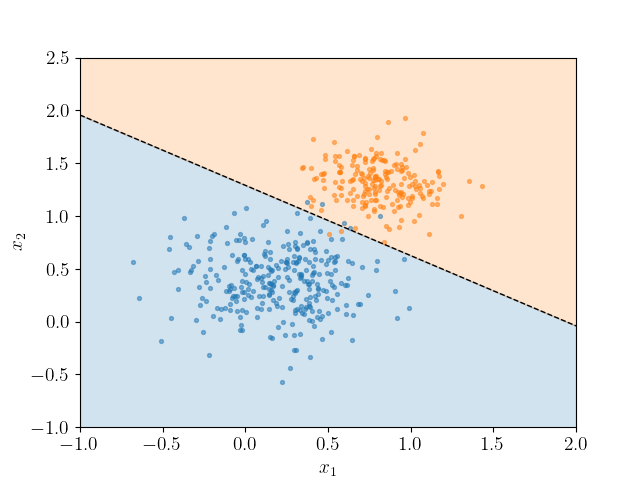
\includegraphics[width=0.7\textwidth]{logistic_regression_boundary.png}
    \captionof{figure}{Hồi quy Logistic học một đường thẳng (hoặc siêu phẳng trong không gian nhiều chiều) để phân chia dữ liệu thành các lớp.}
    \label{fig:logistic_regression_boundary}
\end{center}

\paragraph{Cơ chế hoạt động}
Cho một vector đầu vào $x$ (ví dụ, vector TF-IDF của tài liệu), mô hình thực hiện 2 bước:
\begin{enumerate}
    \item \textbf{Tính toán điểm số tuyến tính (Linear Score):} Mô hình tính một tổng có trọng số của các đặc trưng đầu vào. Mỗi đặc trưng $x_j$ (tương ứng với một từ trong từ vựng) có một trọng số $w_j$.
    $$ z = w_0 + w_1 x_1 + w_2 x_2 + \dots + w_m x_m = w^T x $$
    Trọng số $w_j$ có thể được diễn giải là: một giá trị dương lớn cho thấy sự hiện diện của từ $j$ làm tăng khả năng tài liệu thuộc lớp tích cực, và ngược lại.
    \item \textbf{Ánh xạ qua hàm Sigmoid:} Điểm số $z$ có thể nhận bất kỳ giá trị thực nào. Để biến nó thành một xác suất (nằm trong khoảng [0, 1]), chúng ta đưa nó qua hàm Sigmoid (còn gọi là hàm logistic).
    $$ \sigma(z) = \frac{1}{1 + e^{-z}} $$
\end{enumerate}
Giá trị đầu ra $\sigma(z)$ chính là xác suất dự đoán $P(c=1|d)$.
\paragraph{Huấn luyện bằng Gradient Descent}
Quá trình huấn luyện của Hồi quy Logistic là tìm ra bộ trọng số $w$ tốt nhất để tối thiểu hóa hàm mất mát \textbf{Cross-Entropy} trên toàn bộ tập dữ liệu huấn luyện. Hàm mất mát cho một điểm dữ liệu $(x, y)$ (với $y \in \{0, 1\}$ là nhãn thật) là:
$$ \mathcal{L}(w) = -[y \log(\sigma(w^T x)) + (1-y) \log(1 - \sigma(w^T x))] $$
Gradient của hàm mất mát này theo trọng số $w$ được tính toán, và sau đó thuật toán \textbf{Gradient Descent} (hoặc các biến thể của nó như SGD, Adam) được sử dụng để cập nhật các trọng số $w$ một cách lặp đi lặp lại cho đến khi hội tụ.

\begin{tcolorbox}[
    title=Đánh giá Hồi quy Logistic,
    colback=blue!5!white, colframe=blue!50!black, fonttitle=\bfseries
]
\textbf{Ưu điểm:}
\begin{itemize}
    \item \textbf{Hiệu quả và mạnh mẽ:} Thường cho kết quả tốt hơn Naive Bayes vì nó không có giả định độc lập ngây thơ.
    \item \textbf{Đầu ra là xác suất:} Cung cấp một thước đo độ tin cậy cho dự đoán.
    \item \textbf{Mô hình diễn giải được:} Giống Naive Bayes, có thể kiểm tra các trọng số $w$ để hiểu tầm quan trọng của các từ.
\end{itemize}
\textbf{Nhược điểm:}
\begin{itemize}
    \item \textbf{Bản chất tuyến tính:} Không thể học được các ranh giới quyết định phi tuyến phức tạp. Tuy nhiên, điều này có thể được khắc phục phần nào bằng cách tạo ra các đặc trưng tương tác.
\end{itemize}
\end{tcolorbox}

\subsubsection{Máy Vector Hỗ trợ (Support Vector Machines - SVMs)}
SVM \cite{cortes1995support} là một thuật toán phân loại mạnh mẽ khác, nhưng thay vì tập trung vào xác suất, nó tập trung vào hình học.

\paragraph{Trực giác cốt lõi}
Mục tiêu của SVM là tìm ra một \textbf{siêu phẳng (hyperplane)} phân tách các lớp dữ liệu sao cho \textbf{lề (margin)} -- khoảng cách từ siêu phẳng đến các điểm dữ liệu gần nhất của mỗi lớp -- là \textbf{lớn nhất có thể (maximum margin)}.

\begin{center}
    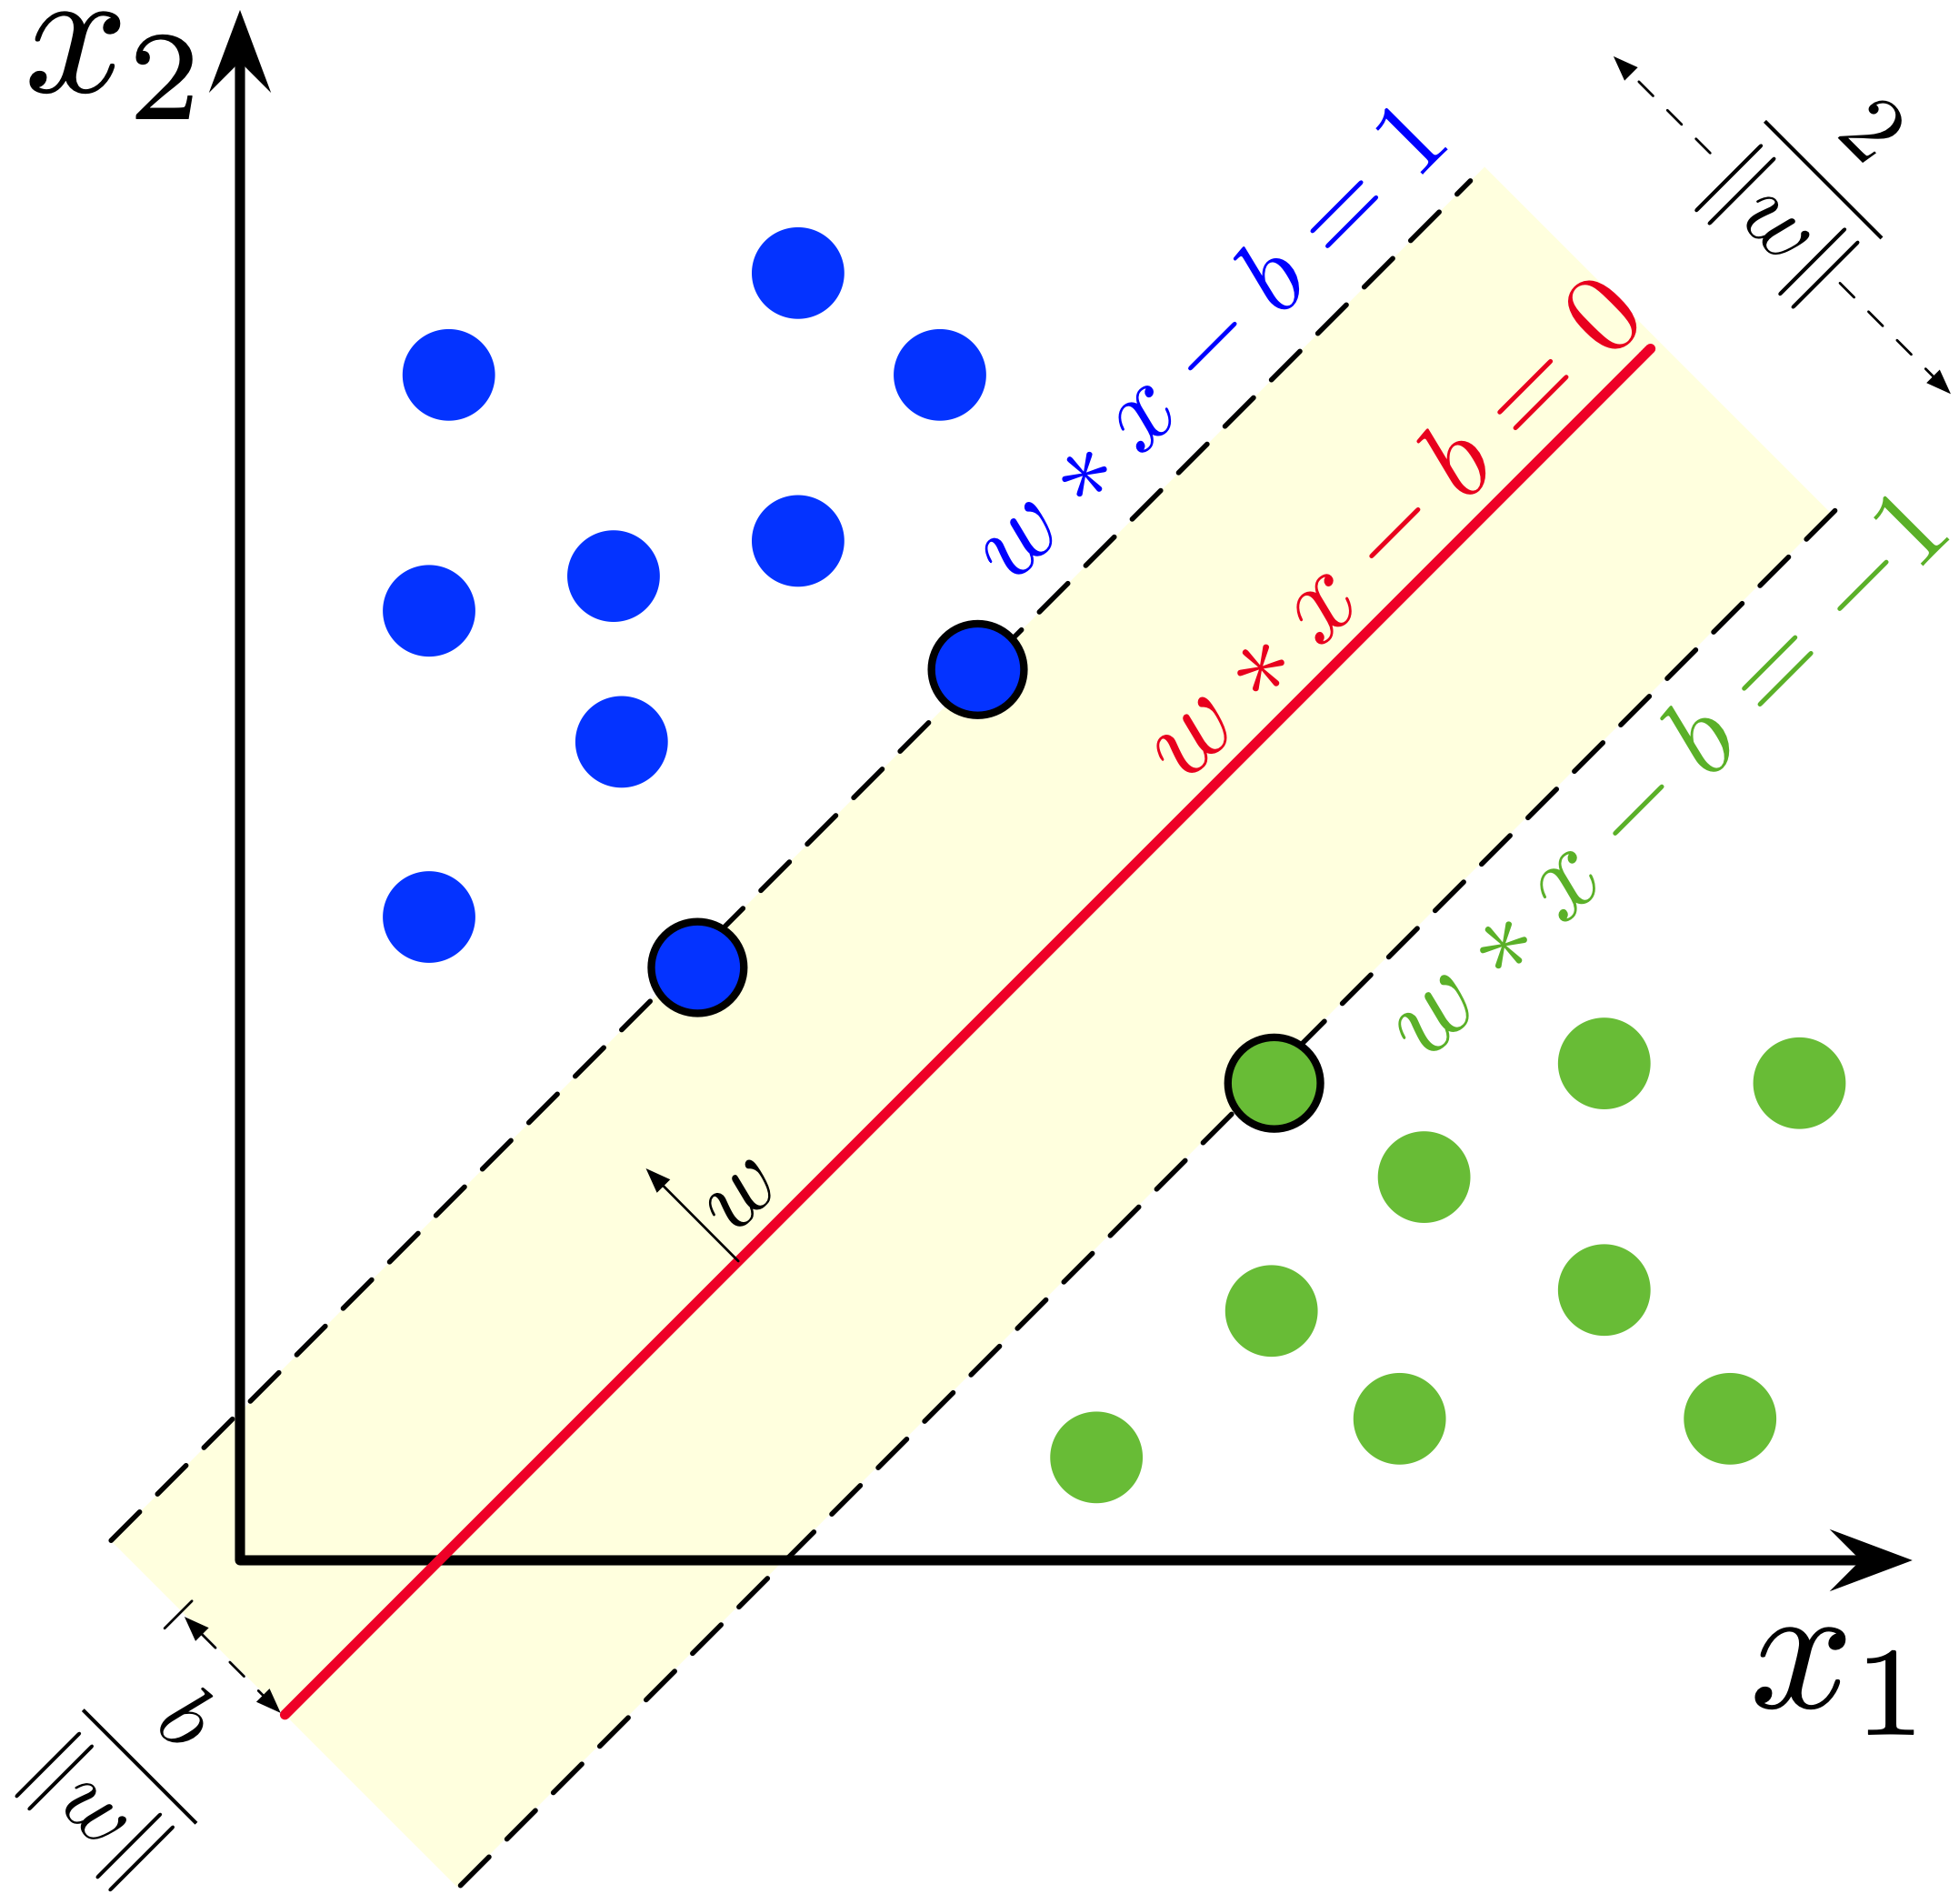
\includegraphics[width=0.7\textwidth]{svm_margin.png}
    \captionof{figure}{SVM tìm siêu phẳng (đường nét đứt) có lề (margin) rộng nhất giữa các lớp. Các điểm nằm trên lề được gọi là các vector hỗ trợ (support vectors).}
    \label{fig:svm_margin}
\end{center}

Việc tối đa hóa lề này giúp mô hình có khả năng tổng quát hóa tốt hơn trên dữ liệu mới, vì ranh giới quyết định ít bị ảnh hưởng bởi nhiễu.

\paragraph{The Kernel Trick}
Điểm mạnh thực sự của SVM nằm ở "thủ thuật kernel" (kernel trick). Nếu dữ liệu không thể phân tách bằng một đường thẳng, SVM có thể sử dụng một hàm kernel (ví dụ: RBF kernel) để ánh xạ dữ liệu lên một không gian nhiều chiều hơn, nơi chúng có thể trở nên phân tách tuyến tính. Điều này cho phép SVM học được các ranh giới quyết định phi tuyến rất phức tạp mà không cần tính toán trực tiếp trong không gian nhiều chiều đó, rất hiệu quả.

\paragraph{Huấn luyện và Hinge Loss}
Quá trình huấn luyện SVM là một bài toán tối ưu hóa nhằm tìm ra siêu phẳng có lề lớn nhất. Điều này được thực hiện bằng cách tối thiểu hóa một hàm mất mát đặc biệt gọi là \textbf{Hinge Loss}:
$$ \mathcal{L}(w) = \max(0, 1 - y_i(w^T x_i - b)) $$
Hàm mất mát này sẽ bằng 0 nếu một điểm dữ liệu nằm đúng phía của lề, và sẽ tăng tuyến tính nếu nó vi phạm lề. Việc tối ưu hóa này thường được giải quyết bằng các phương pháp phức tạp hơn như Quy hoạch toàn phương (Quadratic Programming).

\begin{tcolorbox}[
    title=Đánh giá SVM,
    colback=blue!5!white, colframe=blue!50!black, fonttitle=\bfseries
]
\textbf{Ưu điểm:}
\begin{itemize}
    \item \textbf{Hiệu quả cao trong không gian nhiều chiều:} Rất phù hợp với các vector TF-IDF có số chiều lớn.
    \item \textbf{Học được các ranh giới phi tuyến phức tạp:} Nhờ vào kernel trick.
    \item \textbf{Ít bị quá khớp (overfitting):} Do nguyên lý tối đa hóa lề.
\end{itemize}
\textbf{Nhược điểm:}
\begin{itemize}
    \item \textbf{Chi phí tính toán cao:} Huấn luyện SVM có thể rất chậm trên các bộ dữ liệu lớn.
    \item \textbf{Mô hình hộp đen (Black box):} Việc diễn giải một mô hình SVM với kernel phi tuyến là rất khó.
    \item \textbf{Nhạy cảm với việc lựa chọn kernel và tham số.}
\end{itemize}
\end{tcolorbox}


\subsection{Các mô hình Học chuỗi (Sequence Labeling Models)}
\label{ssec:sequence_models}
Các bài toán như Gán nhãn Từ loại (POS Tagging) hay Nhận dạng Thực thể Tên (NER) không chỉ đơn thuần là phân loại từng từ một cách độc lập. Nhãn của một từ phụ thuộc rất nhiều vào nhãn của các từ xung quanh. Các mô hình học chuỗi được thiết kế để giải quyết vấn đề này.

\subsubsection{Mô hình Markov ẩn (Hidden Markov Models - HMMs)}
HMM \cite{rabiner1989tutorial} là một mô hình sinh kinh điển cho các bài toán gán nhãn chuỗi.

\paragraph{Trực giác cốt lõi}
HMM giả định rằng một chuỗi các quan sát (observations) - tức là các từ trong câu - được "sinh ra" bởi một chuỗi các trạng thái ẩn (hidden states) - tức là các nhãn (ví dụ, các nhãn POS).
Quá trình sinh này tuân theo hai loại xác suất:
\begin{enumerate}
    \item \textbf{Xác suất chuyển trạng thái (Transition Probabilities):} Xác suất chuyển từ một trạng thái ẩn này sang một trạng thái ẩn khác. Ví dụ, $P(\text{Verb}|\text{Noun})$ - xác suất một động từ xuất hiện sau một danh từ. Điều này tuân theo giả định Markov.
    \item \textbf{Xác suất phát sinh (Emission Probabilities):} Xác suất một trạng thái ẩn "sinh ra" một từ quan sát được. Ví dụ, $P(\text{``sách''}|\text{Noun})$ - xác suất từ "sách" được sinh ra khi trạng thái ẩn là Danh từ.
\end{enumerate}

\begin{center}
    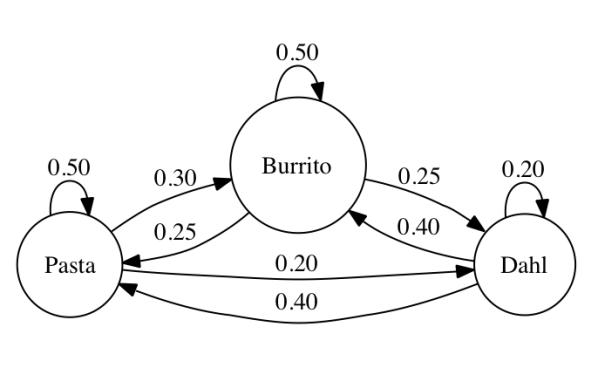
\includegraphics[width=0.8\textwidth]{hmm_diagram.png}
    \captionof{figure}{Sơ đồ một chuỗi Markov (Markov chain) với ba trạng thái: Pasta, Burrito, và Dahl. Các con số biểu thị xác suất chuyển đổi giữa các trạng thái.}
    \label{fig:hmm_diagram}
\end{center}

Nhiệm vụ của HMM là tìm ra chuỗi trạng thái ẩn (chuỗi nhãn) có khả năng nhất đã sinh ra chuỗi các từ quan sát được. Bài toán này được giải quyết hiệu quả bằng một thuật toán quy hoạch động gọi là \textbf{Thuật toán Viterbi (Viterbi Algorithm)}.

\subsubsection{Trường Ngẫu nhiên Có điều kiện (Conditional Random Fields - CRFs)}
CRF, và đặc biệt là Linear-chain CRF, là một cải tiến vượt bậc so với HMM và đã trở thành mô hình thống kê tiêu chuẩn cho các bài toán gán nhãn chuỗi trong nhiều năm.

\paragraph{Sự khác biệt chính với HMM}
HMM là một mô hình sinh, nó mô hình hóa xác suất kết hợp $P(\text{chuỗi quan sát, chuỗi nhãn})$. CRF là một mô hình phân biệt, nó mô hình hóa trực tiếp xác suất có điều kiện $P(\text{chuỗi nhãn}|\text{chuỗi quan sát})$.
Sự thay đổi này mang lại hai lợi thế lớn:
\begin{enumerate}
    \item \textbf{Bỏ giả định độc lập của đặc trưng:} HMM giả định rằng một từ quan sát chỉ phụ thuộc vào trạng thái ẩn hiện tại. CRF không có giả định này. Nó có thể sử dụng một loạt các đặc trưng phức tạp của chuỗi đầu vào, ví dụ: "từ hiện tại có viết hoa không?", "hậu tố của từ hiện tại là gì?", "từ trước đó là gì?". Điều này làm cho CRF linh hoạt và mạnh mẽ hơn nhiều.
    \item \textbf{Tránh tính toán $P(\text{chuỗi quan sát})$:} Việc mô hình hóa xác suất của chuỗi quan sát là rất khó, CRF đã loại bỏ được gánh nặng này.
\end{enumerate}

\paragraph{Trực giác cốt lõi của CRF}
Thay vì tính toán các xác suất chuyển và phát sinh riêng lẻ, một CRF gán một điểm số (score) cho mỗi cặp (chuỗi quan sát, chuỗi nhãn) dựa trên một tổ hợp tuyến tính của các hàm đặc trưng (feature functions). Các hàm đặc trưng này có thể bắt các mối quan hệ phức tạp giữa các từ và nhãn. Sau đó, nó sử dụng một hàm chuẩn hóa (tương tự softmax) trên toàn bộ các chuỗi nhãn có thể có để biến điểm số thành xác suất. Nhiệm vụ cũng là tìm ra chuỗi nhãn có xác suất (điểm số) cao nhất, và cũng thường được giải bằng thuật toán Viterbi.

\begin{tcolorbox}[
    title=So sánh HMM và CRF,
    colback=green!5!white, colframe=green!60!black, fonttitle=\bfseries
]
\begin{tabular}{p{0.45\linewidth} | p{0.45\linewidth}}
    \textbf{Hidden Markov Models (HMM)} & \textbf{Conditional Random Fields (CRF)} \\
    \hline
    Mô hình \textbf{sinh} (Generative) & Mô hình \textbf{phân biệt} (Discriminative) \\
    \hline
    Mô hình hóa $P(\text{observations, labels})$ & Mô hình hóa $P(\text{labels | observations})$ \\
    \hline
    Giả định các quan sát độc lập có điều kiện & Không có giả định độc lập, cho phép các đặc trưng chồng chéo, phức tạp. \\
    \hline
    Huấn luyện nhanh hơn & Huấn luyện chậm hơn (cần các thuật toán lặp) \\
    \hline
    Thường cho hiệu năng thấp hơn & Thường cho hiệu năng \textbf{vượt trội}, là state-of-the-art trong kỷ nguyên thống kê. \\
\end{tabular}
\end{tcolorbox}
% % !TEX root = ../../main.tex
% File: part2/chapters2/chap2_4.tex

\section{Huấn luyện Phân tán (Distributed Training)}
\label{sec:distributed_training}

Khi quy mô của các mô hình ngôn ngữ tăng từ hàng trăm triệu lên hàng tỷ, thậm chí hàng nghìn tỷ tham số, việc huấn luyện chúng trên một GPU duy nhất trở nên bất khả thi. Ngay cả những GPU mạnh nhất cũng không đủ bộ nhớ (VRAM) để chứa toàn bộ trọng số, gradient, và trạng thái của optimizer.

\textbf{Huấn luyện Phân tán} là một tập hợp các kỹ thuật cho phép chúng ta chia nhỏ gánh nặng tính toán và bộ nhớ của quá trình huấn luyện ra \textbf{nhiều GPU} (trên một hoặc nhiều máy).

\subsection{Các Mô hình Song song (Parallelism Paradigms)}
\label{ssec:parallelism_paradigms}
Có nhiều cách khác nhau để "chia nhỏ" quá trình huấn luyện. Ba chiến lược chính là:

\begin{enumerate}
    \item \textbf{Data Parallelism (DP) - Song song Dữ liệu:}
        \begin{itemize}
            \item \textbf{Ý tưởng:} Đây là chiến lược phổ biến và đơn giản nhất. Mỗi GPU sẽ giữ một \textbf{bản sao đầy đủ của mô hình}. Dữ liệu huấn luyện (batch) sẽ được chia nhỏ ra, và mỗi GPU sẽ xử lý một phần của batch đó.
            \item \textbf{Quy trình:} Các GPU tính toán gradient một cách độc lập trên phần dữ liệu của mình, sau đó chúng "giao tiếp" với nhau để đồng bộ hóa và tính trung bình các gradient trước khi cập nhật trọng số.
            \item \textbf{Hạn chế:} Không giải quyết được vấn đề bộ nhớ. Nếu mô hình quá lớn để vừa trên một GPU, DP sẽ không hoạt động.
        \end{itemize}
    \item \textbf{Tensor Parallelism (TP) - Song song Tensor:}
        \begin{itemize}
            \item \textbf{Ý tưởng:} Thay vì sao chép mô hình, chúng ta chia nhỏ \textbf{chính các ma trận trọng số} của mô hình ra nhiều GPU.
            \item \textbf{Quy trình:} Ví dụ, một phép nhân ma trận lớn có thể được chia thành nhiều phép nhân ma trận nhỏ hơn được thực hiện song song trên các GPU khác nhau. Các GPU cần giao tiếp với nhau rất nhiều trong quá trình truyền thẳng và truyền ngược.
            \item \textbf{Lợi ích:} Cho phép huấn luyện các mô hình lớn hơn bộ nhớ của một GPU.
        \end{itemize}
    \item \textbf{Pipeline Parallelism (PP) - Song song Đường ống:}
        \begin{itemize}
            \item \textbf{Ý tưởng:} Chia các \textbf{lớp (layers)} của mô hình ra nhiều GPU.
            \item \textbf{Quy trình:} GPU 1 sẽ xử lý các lớp đầu tiên (ví dụ: 0-11), sau đó chuyển kết quả đầu ra cho GPU 2 để xử lý các lớp tiếp theo (ví dụ: 12-23), và cứ thế tiếp tục. Nó hoạt động giống như một dây chuyền lắp ráp.
            \item \textbf{Hạn chế:} Có thể gây ra "bong bóng" (bubbles), tức là thời gian chờ khi các GPU ở đầu đường ống phải đợi các GPU ở cuối hoàn thành công việc.
        \end{itemize}
\end{enumerate}

Trong thực tế, các hệ thống huấn luyện LLM quy mô lớn thường kết hợp cả ba loại song song này (cùng với các kỹ thuật khác) để đạt được hiệu quả cao nhất.

\subsection{Sử dụng `accelerate` và `DeepSpeed` để Huấn luyện Mô hình lớn}
\label{ssec:accelerate_deepspeed}
Việc triển khai các chiến lược song song này từ đầu là cực kỳ phức tạp. May mắn thay, chúng ta có các thư viện mạnh mẽ giúp tự động hóa quá trình này.

\subsubsection{Accelerate: Giao diện Tối giản}
Như đã giới thiệu ở mục \ref{ssec:hf_accelerate}, `accelerate` cung cấp một giao diện đơn giản để chạy code PyTorch trên nhiều môi trường phần cứng.
\begin{itemize}
    \item \textbf{Cách hoạt động:}
        \begin{enumerate}
            \item Bạn viết một kịch bản huấn luyện PyTorch tiêu chuẩn.
            \item Chạy lệnh `accelerate config` trong terminal để thiết lập môi trường của bạn (ví dụ: "sử dụng 2 GPU trên máy này", "sử dụng precision fp16").
            \item Chạy kịch bản của bạn bằng lệnh `accelerate launch your\_script.py`.
        \end{enumerate}
    \item \textbf{Tích hợp với `Trainer`:} `Trainer` của Hugging Face đã tích hợp sẵn `accelerate`. Khi bạn chạy một kịch bản `Trainer` với `accelerate launch`, nó sẽ tự động áp dụng chiến lược Data Parallelism (DP) trên các GPU có sẵn.
\end{itemize}
`accelerate` là lựa chọn tuyệt vời để dễ dàng song song hóa dữ liệu. Nhưng khi mô hình trở nên quá lớn, chúng ta cần một công cụ mạnh mẽ hơn.

\subsubsection{DeepSpeed: Cỗ máy Tối ưu hóa Toàn diện}
DeepSpeed là một thư viện mã nguồn mở từ Microsoft, cung cấp một bộ công cụ tối ưu hóa cực kỳ mạnh mẽ để huấn luyện các mô hình khổng lồ. Nó không chỉ là một chiến lược song song, mà là một hệ thống toàn diện.

\begin{tcolorbox}[
    title=ZeRO: Tối ưu hóa Bộ nhớ Cách mạng,
    colback=green!5!white, colframe=green!60!black, fonttitle=\bfseries
]
Phát kiến cốt lõi của DeepSpeed là \textbf{ZeRO (Zero Redundancy Optimizer)}. ZeRO nhận ra rằng trong Data Parallelism thông thường, mỗi GPU đều lưu trữ một cách thừa thãi các bản sao của \textbf{trọng số mô hình}, \textbf{gradient}, và \textbf{trạng thái optimizer}. ZeRO loại bỏ sự thừa thãi này bằng cách \textbf{phân mảnh (partitioning)} các thành phần này ra tất cả các GPU.
\end{tcolorbox}

\paragraph{Các Giai đoạn của ZeRO}
\begin{itemize}
    \item \textbf{ZeRO-1:} Phân mảnh \textbf{trạng thái optimizer}. Mỗi GPU chỉ giữ một phần của trạng thái optimizer. Giảm bộ nhớ đáng kể.
    \item \textbf{ZeRO-2:} Phân mảnh cả \textbf{trạng thái optimizer} và \textbf{gradient}. Mỗi GPU chỉ tính và lưu trữ một phần của gradient. Giảm bộ nhớ nhiều hơn nữa.
    \item \textbf{ZeRO-3:} Phân mảnh tất cả: \textbf{trạng thái optimizer}, \textbf{gradient}, và cả \textbf{trọng số mô hình}. Mỗi GPU chỉ giữ một lát cắt (slice) của mô hình. Trong quá trình truyền thẳng/ngược, các GPU sẽ giao tiếp với nhau để tập hợp lại các lớp cần thiết ngay khi cần. Đây là giai đoạn mạnh mẽ nhất, cho phép huấn luyện các mô hình nghìn tỷ tham số.
\end{itemize}

\begin{center}
    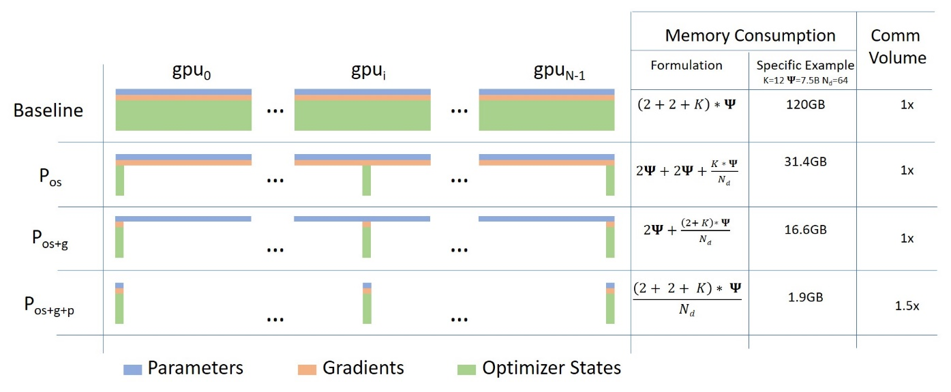
\includegraphics[width=1.0\textwidth]{deepspeed_zero.png}
    \captionof{figure}{So sánh việc sử dụng bộ nhớ trong Data Parallelism tiêu chuẩn và các giai đoạn của ZeRO. ZeRO giảm đáng kể sự thừa thãi bằng cách phân mảnh các thành phần của quá trình huấn luyện.}
    \label{fig:deepspeed_zero}
\end{center}

\paragraph{Tích hợp DeepSpeed với `Trainer`}
Sức mạnh của hệ sinh thái Hugging Face là việc tích hợp các công cụ phức tạp này trở nên rất đơn giản.
\begin{enumerate}
    \item \textbf{Tạo file cấu hình DeepSpeed:} Tạo một file JSON (ví dụ: `ds\_config.json`) để định nghĩa các thiết lập bạn muốn sử dụng (ví dụ: bật ZeRO-2, sử dụng precision fp16, thiết lập optimizer).
    \item \textbf{Truyền vào `TrainingArguments`:}
        \begin{tcolorbox}[title=Cấu hình DeepSpeed, colback=black!5!white, colframe=black!80!white]
            \begin{minted}[linenos, numbersep=0pt]{python}
            training_args = TrainingArguments(
                output_dir="./results",
                # ...
                deepspeed="path/to/your/ds_config.json", # Chỉ định file config
            )
            \end{minted}
        \end{tcolorbox}
    \item \textbf{Khởi chạy:} Sử dụng `deepspeed your\_script.py` hoặc `accelerate launch --use\_deepspeed your\_script.py` để chạy kịch bản.
\end{enumerate}
`Trainer` và `accelerate` sẽ tự động xử lý tất cả các chi tiết phức tạp của việc khởi tạo và chạy DeepSpeed.

Ngoài ZeRO, DeepSpeed còn cung cấp nhiều tính năng tối ưu hóa khác như \textbf{Offloading} (chuyển bớt các tham số không dùng đến từ VRAM sang CPU RAM hoặc NVMe) và các kernel hiệu năng cao. Bằng cách kết hợp các công cụ như `accelerate` và `DeepSpeed`, việc huấn luyện các mô hình ngôn ngữ lớn không còn là đặc quyền của một vài phòng thí nghiệm AI lớn, mà đã trở nên dễ tiếp cận hơn với cộng đồng nghiên cứu và các doanh nghiệp.

\bigskip
\hrule
\bigskip

\begin{center}
    \textbf{\Large KẾT THÚC CHƯƠNG 2}
\end{center}

\textit{Chương 2 đã trang bị cho bạn một bộ công cụ thực chiến hoàn chỉnh, từ việc làm quen với hệ sinh thái Hugging Face, xây dựng các quy trình đánh giá đáng tin cậy, đến việc quản lý các thí nghiệm một cách khoa học và huấn luyện các mô hình trên quy mô lớn. Với những kỹ năng này, bạn đã sẵn sàng để đối mặt với những thách thức phức tạp hơn trong việc triển khai và vận hành các hệ thống NLP trong môi trường production, chủ đề của chương tiếp theo.}

% \chapter{CÁC KIẾN TRÚC MẠNG NƠ-RON KINH ĐIỂN}
\label{chap:deep_learning_architectures}

Chào mừng bạn đến với kỷ nguyên học sâu của NLP. Trong chương 2, chúng ta đã thấy các mô hình thống kê như N-gram có thể nắm bắt các phụ thuộc cục bộ, nhưng lại bất lực trước các mối quan hệ tầm xa. Cuộc cách mạng word embedding đã cho chúng ta các vector từ mang đầy ngữ nghĩa, nhưng làm thế nào để kết hợp chúng lại nhằm hiểu được ý nghĩa của cả một câu hay một đoạn văn?

Chương này sẽ giới thiệu các kiến trúc mạng nơ-ron nền tảng được thiết kế đặc biệt để xử lý dữ liệu dạng chuỗi như ngôn ngữ tự nhiên. Những kiến trúc này không chỉ đơn thuần "nhìn" vào các từ một cách riêng lẻ, mà còn có khả năng "ghi nhớ" và "lý luận" dựa trên thông tin đã xử lý trước đó, cho phép chúng nắm bắt được ngữ cảnh và các phụ thuộc phức tạp trong câu.
% % !TEX root = ../main.tex
% File: chapters_part1/chap3_1.tex
% Nội dung cho Phần 3.1: Word Embeddings

\section{Word Embeddings: Cuộc cách mạng Biểu diễn Đầu tiên}
\label{sec:word_embeddings}

Các phương pháp biểu diễn dựa trên tần suất như BoW hay TF-IDF, mặc dù hữu ích, lại mắc phải hai nhược điểm chí mạng:
\begin{enumerate}
    \item \textbf{Độ thưa thớt (Sparsity):} Chúng tạo ra các vector có số chiều khổng lồ và hầu hết là số 0.
    \item \textbf{Thiếu vắng ngữ nghĩa (Lack of Semantics):} Các vector này không hề nắm bắt được mối quan hệ ngữ nghĩa giữa các từ. Đối với BoW, hai từ "tốt" và "tuyệt vời" là hoàn toàn khác biệt, không có mối liên hệ nào.
\end{enumerate}

\textbf{Word Embeddings} (Nhúng từ) ra đời để giải quyết triệt để hai vấn đề trên. Đây là một tập hợp các kỹ thuật học máy có mục tiêu biểu diễn mỗi từ trong từ vựng bằng một \textbf{vector dày đặc (dense vector)} có số chiều tương đối thấp (thường từ 50 đến 300 chiều). Quan trọng hơn, các vector này được học sao cho chúng có thể nắm bắt được các mối quan hệ ngữ nghĩa và cú pháp giữa các từ.

Ý tưởng nền tảng của Word Embeddings dựa trên \textbf{Giả thuyết Phân bố (Distributional Hypothesis)} của Firth (1957), được tóm gọn trong câu nói nổi tiếng:
\begin{tcolorbox}[
    title=Giả thuyết Phân bố,
    colback=yellow!10!white, colframe=yellow!50!black, fonttitle=\bfseries
]
"You shall know a word by the company it keeps." (Bạn có thể hiểu một từ qua những từ thường đi cùng với nó.)
\end{tcolorbox}
Nói cách khác, những từ xuất hiện trong các ngữ cảnh tương tự nhau thì có khả năng mang ý nghĩa tương tự nhau. Word Embeddings là hiện thực hóa của giả thuyết này bằng các mô hình mạng nơ-ron.

\subsection{Lý thuyết Word2Vec: CBOW \& Skip-gram}
\label{ssec:word2vec}
Được giới thiệu bởi Tomas Mikolov và các cộng sự tại Google vào năm 2013 \cite{mikolov2013efficient, mikolov2013distributed}, Word2Vec không phải là một thuật toán duy nhất mà là một bộ công cụ bao gồm hai kiến trúc mô hình chính: \textbf{CBOW (Continuous Bag-of-Words)} và \textbf{Skip-gram}. Word2Vec đã tạo ra một cuộc cách mạng trong lĩnh vực Xử lý Ngôn ngữ Tự nhiên (NLP), dân chủ hóa việc sử dụng \textit{word embeddings} nhờ vào hiệu quả tính toán và chất lượng của vector biểu diễn mà nó tạo ra.

\subsubsection{Kiến trúc chung: Mạng Nơ-ron Nông}
\label{sssec:w2v_architecture}
Cốt lõi của Word2Vec là một ý tưởng đơn giản đến bất ngờ: thay vì xây dựng một mô hình ngôn ngữ phức tạp, chúng ta thiết kế một nhiệm vụ "giả" (fake task) và trong quá trình huấn luyện mô hình để giải quyết nhiệm vụ đó, chúng ta sẽ học được các vector từ chất lượng cao.

\paragraph{Nhiệm vụ "giả" so với Mô hình Ngôn ngữ "thật"}
Gọi là "giả" vì mục tiêu cuối cùng của chúng ta không phải là giải quyết tốt nhiệm vụ dự đoán từ, mà là học được ma trận trọng số \textbf{W}. Một mô hình ngôn ngữ "thật" (true language model), chẳng hạn như các mô hình dựa trên RNN, sẽ có mục tiêu phức tạp hơn nhiều: dự đoán từ tiếp theo dựa trên toàn bộ lịch sử các từ trước đó ($P(w_t | w_1, ..., w_{t-1})$). Việc này đòi hỏi kiến trúc sâu và phức tạp hơn.

Ngược lại, Word2Vec đơn giản hóa triệt để vấn đề: nó chỉ dự đoán từ dựa trên một cửa sổ ngữ cảnh cục bộ nhỏ. Sự đơn giản hóa này chính là chìa khóa thành công: nó cho phép mô hình xử lý hiệu quả một lượng dữ liệu văn bản khổng lồ. Gradient từ nhiệm vụ đơn giản này, tuy không hoàn hảo cho việc dự đoán ngôn ngữ, lại cực kỳ hiệu quả trong việc định hình một không gian vector mà ở đó các từ có ngữ cảnh tương tự được đặt gần nhau.

Cả CBOW và Skip-gram đều sử dụng kiến trúc mạng nơ-ron "nông" (shallow) chỉ với một lớp ẩn duy nhất. Giả sử từ vựng của chúng ta có \textbf{V} từ độc nhất và chúng ta muốn học các vector biểu diễn có \textbf{N} chiều (embedding dimension).

\begin{itemize}
    \item \textbf{Lớp vào (Input Layer):} Đầu vào là một vector \textit{one-hot} có kích thước $1 \times V$, đại diện cho một từ.
    \item \textbf{Lớp ẩn (Hidden Layer):} Không có hàm kích hoạt. Điểm mấu chốt nằm ở ma trận trọng số \textbf{W} kết nối lớp vào và lớp ẩn. Ma trận này có kích thước $V \times N$.
    \item \textbf{Lớp ra (Output Layer):} Ma trận trọng số \textbf{W'} kết nối lớp ẩn và lớp ra, có kích thước $N \times V$.
\end{itemize}

\begin{tcolorbox}[
    title=Ghi chú về Thiết kế Kiến trúc,
    colback=green!5!white, colframe=green!50!black, fonttitle=\bfseries
]
\textbf{1. Tại sao không có hàm kích hoạt ở lớp ẩn?} \\
Lớp ẩn của Word2Vec thực chất là một lớp tuyến tính (linear projection). Việc loại bỏ hàm phi tuyến (như ReLU hay Tanh) là một lựa chọn có chủ ý. Mục đích là để các mối quan hệ ngữ nghĩa (ví dụ: các phép loại suy -- analogies) có thể được biểu diễn dưới dạng các phép toán vector tuyến tính đơn giản (ví dụ: $\vec{v}_{\text{king}} - \vec{v}_{\text{man}} + \vec{v}_{\text{woman}} \approx \vec{v}_{\text{queen}}$). Nếu thêm hàm phi tuyến, cấu trúc tuyến tính này sẽ bị phá vỡ, làm cho các vector học được khó diễn giải và sử dụng hơn theo cách này. Lớp ẩn chỉ đóng vai trò như một bảng tra cứu (lookup table) để lấy ra vector embedding.

\textbf{2. Tại sao có hai ma trận trọng số W và W'?} \\
Mô hình có hai bộ vector cho mỗi từ:
\begin{itemize}
    \item \textbf{Input vectors (trong W):} Khi từ được dùng làm đầu vào (từ trung tâm trong Skip-gram, từ ngữ cảnh trong CBOW).
    \item \textbf{Output vectors (trong W'):} Khi từ được dùng làm mục tiêu dự đoán (từ ngữ cảnh trong Skip-gram, từ trung tâm trong CBOW).
\end{itemize}
Về mặt lý thuyết, việc có hai vai trò riêng biệt cho phép mô hình linh hoạt hơn. Sau khi huấn luyện xong, chúng ta thường chỉ sử dụng ma trận đầu vào \textbf{W} làm embedding cuối cùng. Đây là một quy ước phổ biến và cho kết quả tốt trong thực tế. Một số nghiên cứu cũng đề xuất các cách kết hợp khác (ví dụ, lấy trung bình cộng của hai vector tương ứng từ \textbf{W} và \textbf{W'}), nhưng chỉ dùng \textbf{W} vẫn là phương pháp tiêu chuẩn.
\end{tcolorbox}

Điều quan trọng là, chúng ta không thực sự quan tâm đến kết quả dự đoán của mạng. Mục tiêu cuối cùng của chúng ta là học được ma trận trọng số \textbf{W}. Sau khi huấn luyện, mỗi hàng của ma trận \textbf{W} chính là vector embedding N-chiều cho một từ tương ứng trong từ vựng. Do đó, \textbf{W} còn được gọi là \textbf{ma trận embedding (embedding matrix)}.

\begin{center}
    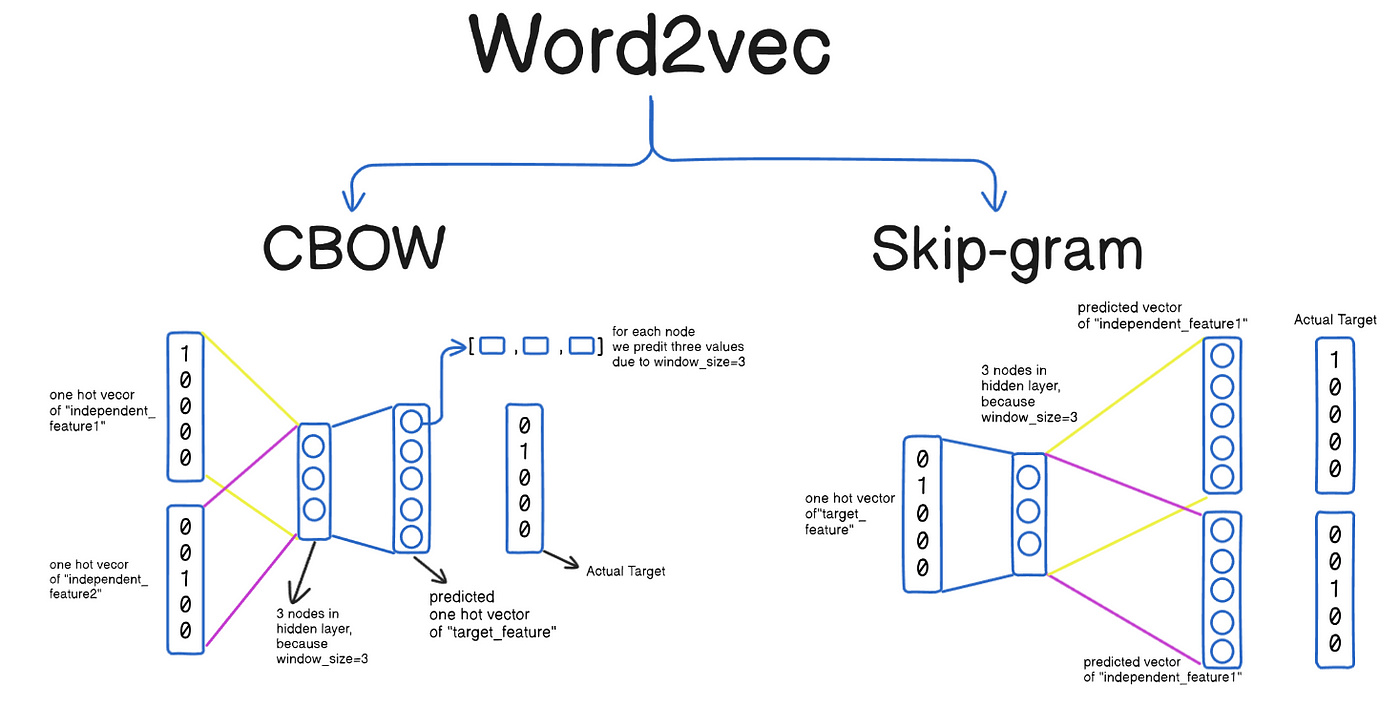
\includegraphics[width=0.8\textwidth]{word2vec_architecture.png}
    \captionof{figure}{Kiến trúc chung của Word2Vec. Khi nhân vector one-hot của một từ với ma trận $W$, thực chất chúng ta đang "chọn" ra hàng tương ứng với từ đó, chính là vector embedding của nó. Ma trận $W$ là mục tiêu chúng ta cần học.}
    \label{fig:word2vec_architecture}
\end{center}

\subsubsection{Mô hình CBOW (Continuous Bag-of-Words)}
\paragraph{Tư duy cốt lõi}
Mô hình CBOW hoạt động dựa trên giả định: "Một từ có thể được dự đoán bởi các từ xung quanh nó". Do đó, CBOW cố gắng \textbf{dự đoán một từ trung tâm (center word) dựa vào các từ ngữ cảnh (context words)}.

Ví dụ, trong câu "chú mèo [ngồi] trên chiếc chiếu" và cửa sổ ngữ cảnh là 2, CBOW sẽ lấy các từ ngữ cảnh \texttt{\{"chú", "mèo", "trên", "chiếc"\}} để dự đoán từ trung tâm là \texttt{\{"ngồi"\}}.

\paragraph{Cơ chế hoạt động}
\begin{enumerate}
    \item \textbf{Đầu vào:} Lấy các vector one-hot của các từ ngữ cảnh (ví dụ: \texttt{chú}, \texttt{mèo}, \texttt{trên}, \texttt{chiếc}).
    \item \textbf{Lấy vector embedding:} Từ ma trận embedding \textbf{W}, ta lấy ra các vector embedding tương ứng cho từng từ ngữ cảnh.
    \item \textbf{Tổng hợp ngữ cảnh:} Các vector embedding này được \textbf{lấy trung bình cộng} để tạo thành một vector ngữ cảnh duy nhất $\mathbf{v}_{\text{context}}$. Việc lấy trung bình này giải thích cho tên gọi "Bag-of-Words", vì nó làm mất đi thông tin về thứ tự các từ trong ngữ cảnh.
    \item \textbf{Dự đoán:} Vector $\mathbf{v}_{\text{context}}$ được nhân với ma trận \textbf{W'} và đưa qua hàm \textbf{softmax} để tạo ra một phân phối xác suất trên toàn bộ từ vựng. Vector đầu ra $\hat{\mathbf{y}}$ có kích thước $1 \times V$, trong đó phần tử thứ $j$ biểu diễn xác suất từ trung tâm là từ thứ $j$ trong từ vựng.
    \item \textbf{Huấn luyện:} So sánh vector xác suất dự đoán $\hat{\mathbf{y}}$ với vector one-hot $\mathbf{y}$ của từ trung tâm thực tế (từ \texttt{ngồi}). Hàm mất mát thường được sử dụng là \textbf{Cross-Entropy}, và lỗi được lan truyền ngược (backpropagation) để cập nhật các trọng số trong cả hai ma trận \textbf{W} và \textbf{W'}.
    $$ \mathcal{L} = -\sum_{j=1}^{V} y_j \log(\hat{y}_j) $$
\end{enumerate}

\paragraph{Phân tích lựa chọn thiết kế của CBOW}
Việc lấy trung bình các vector ngữ cảnh là một lựa chọn thiết kế vì sự đơn giản và hiệu quả tính toán. Nó không cần tham số nào để học và có thể được tính rất nhanh. Tuy nhiên, lựa chọn này có hai hệ quả quan trọng:
\begin{itemize}
    \item \textbf{Mất thông tin thứ tự:} CBOW không phân biệt được hai câu có cùng các từ ngữ cảnh nhưng khác trật tự. Trong nhiều tác vụ, việc mất thông tin cú pháp này là một hạn chế đáng kể.
    \item \textbf{"Lu mờ" từ hiếm:} Khi lấy trung bình, đóng góp của một vector từ hiếm có thể bị "lấn át" bởi các vector của các từ ngữ cảnh phổ biến hơn. Đây là lý do CBOW thường hoạt động kém hơn Skip-gram đối với các từ hiếm.
\end{itemize}
Các phương pháp phức tạp hơn như lấy trung bình có trọng số (dựa trên khoảng cách tới từ trung tâm) hoặc thậm chí dùng một cơ chế attention đơn giản có thể được xem xét, nhưng chúng sẽ làm tăng độ phức tạp và đi ngược lại triết lý "đơn giản, nhanh" của Word2Vec.

\subsubsection{Mô hình Skip-gram}
\paragraph{Tư duy cốt lõi}
Skip-gram đảo ngược lại nhiệm vụ của CBOW. Nó hoạt động dựa trên giả định: "Một từ có thể cho biết những từ nào sẽ xuất hiện xung quanh nó". Do đó, Skip-gram cố gắng \textbf{dự đoán các từ ngữ cảnh dựa vào một từ trung tâm}.

Ví dụ, với cùng câu trên, Skip-gram sẽ lấy từ trung tâm \texttt{\{"ngồi"\}} để cố gắng dự đoán từng từ trong tập ngữ cảnh \texttt{\{"chú", "mèo", "trên", "chiếc"\}}.

\paragraph{Cơ chế hoạt động}
Khác với CBOW, Skip-gram không gộp ngữ cảnh lại. Thay vào đó, nó tạo ra nhiều mẫu huấn luyện hơn từ một cửa sổ ngữ cảnh.
\begin{enumerate}
    \item \textbf{Đầu vào:} Lấy vector one-hot của từ trung tâm (ví dụ: \texttt{ngồi}).
    \item \textbf{Lấy vector embedding:} Lấy ra vector embedding $\mathbf{v}_{\text{center}}$ của từ trung tâm từ ma trận \textbf{W}.
    \item \textbf{Dự đoán:} Vector $\mathbf{v}_{\text{center}}$ được đưa thẳng đến lớp ra (nhân với \textbf{W'} và qua hàm softmax) để tạo ra một vector xác suất $\hat{\mathbf{y}}$.
    \item \textbf{Huấn luyện:} Quá trình này được lặp lại cho \textbf{từng từ trong ngữ cảnh}. Với mỗi cặp (\texttt{từ trung tâm}, \texttt{từ ngữ cảnh}), một hàm mất mát \textbf{Cross-Entropy} được tính toán giữa dự đoán $\hat{\mathbf{y}}$ và vector one-hot của từ ngữ cảnh thực tế. Tổng các lỗi từ tất cả các cặp được sử dụng để cập nhật trọng số qua backpropagation. Điều này giúp Skip-gram học được các biểu diễn tinh vi hơn, đặc biệt cho các từ hiếm, nhưng cũng tốn nhiều thời gian huấn luyện hơn.
\end{enumerate}

\begin{center}
    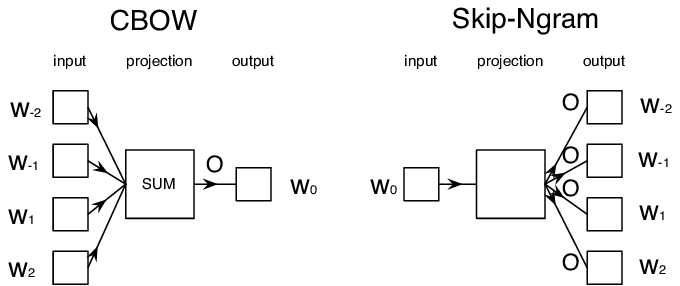
\includegraphics[width=0.9\textwidth]{cbow_skipgram_diagram.png}
    \captionof{figure}{So sánh trực quan giữa CBOW (tổng hợp ngữ cảnh để dự đoán 1 từ) và Skip-gram (dùng 1 từ để dự đoán nhiều từ trong ngữ cảnh, tạo thành các cặp huấn luyện riêng biệt).}
    \label{fig:cbow_skipgram_diagram}
\end{center}

\subsubsection{Vì sao Word2Vec học được ngữ nghĩa và gần--xa theo cosine?}
\label{sssec:w2v_why_semantics}

\paragraph{Nguyên lý phân bố (Distributional Hypothesis).}
Từ ngữ xuất hiện trong \emph{ngữ cảnh} giống nhau thường có nghĩa giống nhau. Khi huấn luyện Word2Vec để dự đoán từ--ngữ cảnh, các vector bị tối ưu sao cho những từ chia sẻ nhiều ngữ cảnh sẽ có \emph{hướng} gần nhau trong không gian.

\paragraph{CBOW: gom ngữ cảnh để dự đoán từ.}
Gọi $C$ là tập ngữ cảnh, $|C|=m$, $v_c \in \mathbb{R}^N$ là embedding của từ $c\in C$, và $u_w \in \mathbb{R}^N$ là vector ``ra'' cho từ trung tâm $w$. CBOW tính
\[
h \;=\; \frac{1}{m}\sum_{c\in C} v_c,\qquad 
p(w\,|\,C) \;=\; \mathrm{softmax}\big(u_w^\top h\big).
\]
Tối đa hoá $\log p(w\,|\,C)$ khiến $u_w^\top h$ tăng. Do $h$ là trung bình các $v_c$, mọi $v_c$ đều nhận gradient đẩy \emph{đồng hướng} với $u_w$. Khi hai từ $w_1,w_2$ thường cùng chia sẻ ngữ cảnh, các cập nhật lặp đi lặp lại làm $v_{w_1},v_{w_2}$ trở nên \emph{đồng hướng}.

\paragraph{Skip-gram với Negative Sampling (SGNS): kéo--đẩy cục bộ.}
Với cặp dương $(w,c)$ và các âm $n\in\mathcal{N}$, hàm mục tiêu một bước là
\[
\mathcal{L}_{\text{SGNS}} \;=\; 
- \log \sigma\!\big(u_c^\top v_w\big) \;-\; \sum_{n\in\mathcal{N}} \log \sigma\!\big(-u_n^\top v_w\big),
\]
trong đó $\sigma(x)=\frac{1}{1+e^{-x}}$. Gradient theo $v_w$ là
\[
\frac{\partial \mathcal{L}}{\partial v_w}
= \big(\sigma(u_c^\top v_w)-1\big)\,u_c \;+\; \sum_{n\in\mathcal{N}} \sigma(u_n^\top v_w)\,u_n.
\]
\emph{Trực giác:} với cặp dương, hệ số $\sigma(u_c^\top v_w)-1<0$ kéo $v_w$ \emph{tiến} về hướng $u_c$ (tăng tích vô hướng); với cặp âm, các hạng $+\sigma(u_n^\top v_w)\,u_n$ đẩy $v_w$ \emph{ra xa} các $u_n$. Qua thời gian, các từ chia sẻ ngữ cảnh dương sẽ bị kéo về \emph{cùng vùng} (gần nhau), còn các từ hiếm khi cùng ngữ cảnh sẽ bị \emph{đẩy xa}.

\paragraph{Vì sao cosine similarity?}
Huấn luyện tối ưu \emph{tích vô hướng} $u^\top v$ (do xuất hiện trong softmax/SGNS). Khi chuẩn hoá độ dài, tối đa hoá tích vô hướng tương đương tối đa hoá \emph{cosine}:
\[
u^\top v \;=\; \|u\|\,\|v\|\,\cos\theta.
\]
Trong thực tế, độ dài có thể dao động, nhưng \emph{hướng} mới mã hoá ``vị trí ngữ nghĩa''. Do đó, dùng cosine để đo gần--xa phản ánh đúng mục tiêu tối ưu hoá hướng.

\paragraph{Gần nghĩa, khác nghĩa, và trái nghĩa.}
\begin{itemize}
    \item \textbf{Gần nghĩa $\Rightarrow$ gần nhau:} nếu hai từ thường xuất hiện với \emph{cùng loại ngữ cảnh}, các cập nhật kéo chúng về \emph{đồng hướng} $\Rightarrow$ cosine cao.
    \item \textbf{Khác nghĩa $\Rightarrow$ xa nhau:} nếu hầu như không chia sẻ ngữ cảnh, vector bị các cập nhật khác hướng $\Rightarrow$ cosine thấp.
    \item \textbf{Trái nghĩa vẫn có thể gần nhau:} các cặp như \textit{nóng}--\textit{lạnh} xuất hiện trong \emph{ngữ cảnh hình thức} tương tự (``thời tiết \underline{nóng}/\underline{lạnh}'') nên vẫn bị kéo về gần nhau; Word2Vec không mô hình hoá \emph{độ phân cực nghĩa}. Muốn phân biệt polarity thường cần thêm tín hiệu (sentiment, lexicon, hoặc mô hình ngôn ngữ ngữ cảnh hoá).
\end{itemize}

\paragraph{Liên hệ lý thuyết: SGNS và Phân rã Ma trận PMI}
Một khám phá lý thuyết quan trọng của Levy và Goldberg \cite{levy2014neural} đã chỉ ra rằng mục tiêu tối ưu của Skip-gram với Negative Sampling (SGNS) thực chất tương đương với việc \textbf{phân rã ngầm định (implicit factorization)} một ma trận đặc biệt.  Cụ thể, hàm mục tiêu của SGNS hội tụ về việc tối ưu hóa sao cho:
\[ \mathbf{w}_i^\top \mathbf{c}_j \approx \text{PMI}(w_i, c_j) - \log k \]
trong đó $\mathbf{w}_i$ và $\mathbf{c}_j$ là các vector đầu vào và đầu ra, $k$ là số mẫu âm, và PMI (Pointwise Mutual Information) là một thước đo mức độ liên quan giữa hai từ:
\[ \text{PMI}(w, c) = \log \frac{P(w, c)}{P(w)P(c)} \]
Phát hiện này kết nối Word2Vec (một mô hình dự đoán, dựa trên mạng nơ-ron) với các phương pháp dựa trên đếm truyền thống (như LSA, GloVe) vốn trực tiếp phân rã ma trận đồng xuất hiện hoặc PMI. Nó cho thấy trực giác "kéo--đẩy" của SGNS không chỉ là một heuristic, mà là một cách hiệu quả để xấp xỉ một cấu trúc thống kê toàn cục của ngôn ngữ, làm sáng tỏ lý do tại sao các mối quan hệ ngữ nghĩa lại có thể được học một cách hiệu quả như vậy.

\paragraph{Hệ quả và giới hạn.}
\begin{itemize}
    \item \textbf{Tổng quát hoá theo ngữ cảnh:} ``nghĩa'' trong Word2Vec chủ yếu là \emph{tương đồng ngữ cảnh} (contextual co-occurrence).
    \item \textbf{Đa nghĩa:} một vector cho nhiều nghĩa sẽ trộn các ngữ cảnh (polysemy). Các mô hình \emph{ngữ cảnh hoá} (ELMo, BERT) khắc phục bằng vector phụ thuộc câu.
    \item \textbf{Cosine là thước đo mặc định:} vì hướng là tín hiệu chính của ``ngữ nghĩa'' đã học qua $u^\top v$.
\end{itemize}

\begin{tcolorbox}[title=Trực giác ``kéo--đẩy'' trong SGNS, colback=blue!5!white, colframe=blue!60!black, fonttitle=\bfseries]
\textbf{Kéo:} cặp dương $(w,c)$ làm tăng $u_c^\top v_w$ $\Rightarrow$ $v_w$ tiến về hướng $u_c$. 
\quad
\textbf{Đẩy:} cặp âm $(w,n)$ làm giảm $u_n^\top v_w$ $\Rightarrow$ $v_w$ rời xa hướng $u_n$.
\\[3pt]
Lặp lại trên toàn corpora tạo ra cấu trúc không gian nơi \emph{các trường ngữ cảnh} được biểu diễn bằng \emph{hướng vector}; cosine đo độ tương đồng các trường ngữ cảnh đó.
\end{tcolorbox}

\subsubsection{Thách thức tính toán và các kỹ thuật tối ưu hóa}
Cả hai mô hình đều đối mặt với một nút thắt cổ chai lớn: hàm \textbf{softmax} ở lớp ra. Việc tính toán mẫu số của hàm softmax đòi hỏi phải duyệt qua toàn bộ \textbf{V} từ trong từ vựng, cực kỳ tốn kém khi V có thể lên tới hàng triệu. Để giải quyết vấn đề này, hai kỹ thuật chính được đề xuất:

\paragraph{Subsampling và Cửa sổ ngữ cảnh động}
Trước khi đi vào các kỹ thuật tối ưu hóa chính, có hai thủ thuật quan trọng khác giúp cải thiện chất lượng embedding và tăng tốc độ huấn luyện:
\begin{itemize}
    \item \textbf{Subsampling các từ thường xuyên:} Các từ xuất hiện rất thường xuyên (như "là", "và", "trong" trong tiếng Việt, hay "the", "a" trong tiếng Anh) mang ít thông tin ngữ nghĩa đặc trưng. Chúng xuất hiện trong gần như mọi ngữ cảnh, do đó các cặp huấn luyện tạo ra từ chúng không giúp ích nhiều mà còn làm chậm quá trình huấn luyện. Subsampling là một kỹ thuật loại bỏ ngẫu nhiên các từ này trong quá trình tạo mẫu, với xác suất loại bỏ càng cao khi tần suất của từ càng lớn. Điều này giúp mô hình tập trung hơn vào các từ hiếm và quan trọng hơn.
    
    \item \textbf{Cửa sổ ngữ cảnh động (Dynamic Window):} Thay vì sử dụng một cửa sổ ngữ cảnh có kích thước cố định (ví dụ, luôn là 5), nhiều triển khai của Word2Vec sử dụng một kích thước cửa sổ động. Với mỗi từ trung tâm, một kích thước cửa sổ $C$ sẽ được chọn ngẫu nhiên trong khoảng từ 1 đến kích thước tối đa cho phép. Kỹ thuật này có tác dụng ngầm định là gán trọng số cao hơn cho các từ ngữ cảnh ở gần từ trung tâm, vì chúng có xác suất được lấy mẫu cao hơn các từ ở xa.
\end{itemize}

\paragraph{Negative Sampling}
Đây là kỹ thuật phổ biến hơn. Thay vì cập nhật trọng số cho toàn bộ từ vựng, ý tưởng là biến bài toán phân loại đa lớp (multi-class) thành một loạt các bài toán phân loại nhị phân (binary classification). Với mỗi cặp đầu vào (ví dụ, trong Skip-gram là \texttt{(từ trung tâm, từ ngữ cảnh)}):
\begin{enumerate}
    \item Chúng ta coi cặp này là một mẫu \textbf{dương tính (positive sample)}.
    \item Chúng ta lấy ngẫu nhiên \textbf{k} từ khác từ từ vựng (dựa trên một phân phối xác suất nhất định) và tạo ra \textbf{k} mẫu \textbf{âm tính (negative samples)}.
    \item Mô hình sẽ được huấn luyện để dự đoán đúng "nhãn" (1 cho mẫu dương tính, 0 cho các mẫu âm tính).
\end{enumerate}
Bằng cách này, trong mỗi bước cập nhật, chúng ta chỉ cần tính toán và cập nhật trọng số cho $k+1$ từ thay vì toàn bộ V từ, giúp tăng tốc độ huấn luyện lên rất nhiều.

\begin{tcolorbox}[
    title=Lựa chọn Thiết kế trong Negative Sampling,
    colback=orange!5!white, colframe=orange!60!black, fonttitle=\bfseries
]
\textbf{1. Phân phối lấy mẫu âm (The Sampling Distribution):} \\
Việc lấy mẫu các từ "âm tính" không phải là ngẫu nhiên đồng nhất trên toàn bộ từ vựng. Thay vào đó, Mikolov đề xuất sử dụng một phân phối Unigram đã được điều chỉnh, trong đó xác suất chọn một từ $w$ làm mẫu âm là:
\[ P(w) = \frac{f(w)^{3/4}}{\sum_{j=1}^{V} f(w_j)^{3/4}} \]
trong đó $f(w)$ là tần suất của từ $w$. Lũy thừa $3/4$ là một heuristic được chọn qua thực nghiệm.
\begin{itemize}
    \item Nếu dùng lũy thừa $1$ (theo tần suất thô), các từ rất phổ biến sẽ được chọn làm mẫu âm quá thường xuyên.
    \item Nếu dùng lũy thừa $0$ (phân phối đều), các từ hiếm sẽ được chọn thường xuyên một cách phi thực tế.
    \item Lũy thừa $3/4$ là một sự cân bằng hợp lý: nó làm giảm nhẹ tần suất của các từ phổ biến và tăng nhẹ tần suất của các từ hiếm, tạo ra các mẫu âm đa dạng và thách thức hơn cho mô hình.
\end{itemize}

\textbf{2. Số lượng mẫu âm (k):} \\
Tham số $k$ (số mẫu âm cho mỗi mẫu dương) thể hiện sự đánh đổi giữa chất lượng và tốc độ.
\begin{itemize}
    \item Với các tập dữ liệu nhỏ, $k$ lớn hơn (ví dụ: 5-20) thường cho kết quả tốt hơn vì mỗi mẫu dương cần nhiều ví dụ âm để mô hình học được ranh giới quyết định.
    \item Với các tập dữ liệu cực lớn, $k$ có thể nhỏ hơn (ví dụ: 2-5), vì mô hình đã thấy đủ đa dạng mẫu trong dữ liệu.
\end{itemize}
Giá trị của $k$ càng lớn, gradient càng ổn định nhưng chi phí tính toán cho mỗi bước cập nhật càng cao.
\end{tcolorbox}

\paragraph{Hierarchical Softmax}
Kỹ thuật này sử dụng một cây nhị phân (cụ thể là cây Huffman) để biểu diễn tất cả các từ trong từ vựng. Các từ thường xuyên xuất hiện sẽ có đường đi ngắn hơn trên cây. Thay vì dự đoán một từ, mô hình sẽ dự đoán một chuỗi các lựa chọn trái/phải để đi từ gốc đến lá của từ đó. Điều này giảm độ phức tạp tính toán từ $O(V)$ xuống còn $O(\log_2V)$.

\begin{tcolorbox}[
    title=So sánh CBOW và Skip-gram,
    colback=blue!5!white, colframe=blue!60!black, fonttitle=\bfseries
]
\begin{tabular}{p{0.45\linewidth} | p{0.45\linewidth}}
    \textbf{CBOW} & \textbf{Skip-gram} \\
    \hline
    Dự đoán từ trung tâm từ ngữ cảnh. & Dự đoán các từ ngữ cảnh từ từ trung tâm. \\
    \hline
    Nhanh hơn, chỉ một lần cập nhật cho mỗi cửa sổ ngữ cảnh. & Chậm hơn, phải cập nhật nhiều lần (mỗi từ trong ngữ cảnh). \\
    \hline
    Kém hiệu quả với từ hiếm do việc lấy trung bình làm “lu mờ” chúng. & Tốt hơn với từ hiếm vì mỗi từ vẫn tạo ra một cặp huấn luyện riêng. \\
    \hline
    Tốt cho các từ thường xuyên xuất hiện. & Thường tốt hơn với dữ liệu lớn và từ hiếm. \\
    \hline
    \textbf{Khi nào dùng?} Khi tốc độ là ưu tiên và dữ liệu rất lớn. & \textbf{Khi nào dùng?} Thường được ưa chuộng trong nghiên cứu vì chất lượng biểu diễn cao. \\
\end{tabular}
\end{tcolorbox}
Nhìn chung, Skip-gram thường được ưa chuộng hơn trong nghiên cứu.

\subsection{Lý thuyết GloVe: Ma trận Đồng xuất hiện}
\label{ssec:glove}

GloVe \cite{pennington2014glove} (\textit{Global Vectors for Word Representation}) được giới thiệu năm 2014 bởi các nhà nghiên cứu tại Stanford như một phương pháp học \textbf{word embeddings} dựa trên thống kê toàn cục của ngôn ngữ. 
Khác với Word2Vec (mô hình \textit{predictive}, học từ các ngữ cảnh cục bộ), GloVe là một mô hình \textit{count-based} được huấn luyện bằng tư duy tối ưu giống mô hình dự đoán, nhằm tận dụng cả thông tin toàn cục và cục bộ.

\paragraph{Tư duy cốt lõi}
Tần suất đồng xuất hiện giữa các từ mang ý nghĩa ngữ nghĩa quan trọng. Ví dụ: từ \textit{ice} và \textit{steam} đều đồng xuất hiện với \textit{water}, nhưng:
\begin{itemize}
    \item \textit{ice} đồng xuất hiện nhiều hơn với \textit{solid}, ít với \textit{gas}.
    \item \textit{steam} đồng xuất hiện nhiều hơn với \textit{gas}, ít với \textit{solid}.
\end{itemize}
So sánh tỉ lệ xác suất đồng xuất hiện giúp phân biệt nghĩa của các từ.

\begin{tcolorbox}[
    title=GloVe: Sự giao thoa giữa Count-based và Predictive,
    colback=green!5!white, colframe=green!50!black, fonttitle=\bfseries
]
Một câu hỏi thường gặp là: Nếu GloVe xây dựng trên ma trận đếm toàn cục, tại sao nó không đơn giản là phân rã ma trận đó (như LSA)? Và nếu hàm mất mát của nó trông giống một bài toán dự đoán, tại sao nó không phải là mô hình predictive như Word2Vec?

Câu trả lời nằm ở chỗ GloVe kết hợp những điểm mạnh của cả hai phương pháp:
\begin{itemize}
    \item \textbf{Tận dụng thống kê toàn cục (Count-based):} Bằng cách tiền tính toán ma trận đồng xuất hiện $X$, GloVe có cái nhìn bao quát về toàn bộ kho văn bản ngay từ đầu. Mọi thông tin về tần suất và sự đồng xuất hiện đều được mã hóa trong ma trận này.
    \item \textbf Tối ưu hóa hiệu quả (Predictive-style): Thay vì thực hiện các phép phân rã ma trận phức tạp và tốn kém (như SVD trong LSA), GloVe định nghĩa một hàm mất mát dạng "hồi quy có trọng số". Mô hình sau đó học các vector bằng cách tối ưu hàm mất mát này trên từng cặp $(i, j)$ không rỗng trong ma trận $X$. Cách học lặp đi lặp lại trên các mẫu riêng lẻ này rất giống với tinh thần của các mô hình dự đoán, giúp việc huấn luyện trở nên hiệu quả và có thể song song hóa.
\end{itemize}
Do đó, GloVe có thể được xem là một mô hình "lai": nó trực tiếp tối ưu hóa để học các vector sao cho chúng có thể tái tạo lại được các thống kê toàn cục của ngôn ngữ.
\end{tcolorbox}

\paragraph{Tỉ lệ xác suất}
Cho từ $i$, $j$ và từ ngữ cảnh $k$, xác suất đồng xuất hiện được định nghĩa:
\[
P_{ik} = \frac{\text{số lần từ $k$ xuất hiện gần $i$}}{\text{tổng số lần xuất hiện ngữ cảnh của $i$}}
\]
GloVe chỉ ra rằng \textbf{tỉ lệ} $\frac{P_{ik}}{P_{jk}}$ chứa thông tin ngữ nghĩa: nếu $k$ liên quan nhiều đến $i$ hơn $j$, tỉ lệ này sẽ lớn.

\paragraph{Từ Tỉ lệ đến Tích vô hướng: Cầu nối Toán học}
Đây là bước nhảy vọt tinh tế nhất của GloVe. Các tác giả đã lập luận như sau:
\begin{enumerate}
    \item Mối quan hệ giữa ba từ $i, j, k$ được thể hiện qua tỉ lệ $P_{ik}/P_{jk}$. Mối quan hệ này nên được mô hình hóa bởi các vector của chúng: $w_i, w_j, w_k$. Ta có thể bắt đầu với một hàm tổng quát $F$:
    \[ F(w_i, w_j, w_k) = \frac{P_{ik}}{P_{jk}} \]
    \item Để mã hóa thông tin trong không gian vector tuyến tính, các tác giả đề xuất rằng $F$ nên chỉ phụ thuộc vào hiệu của hai từ đầu tiên, $F(w_i - w_j, w_k)$. Điều này giúp nắm bắt các mối quan hệ loại suy (analogy).
    \item Để đơn giản hóa hơn nữa, họ nhận thấy rằng vế phải là một đại lượng vô hướng, trong khi vế trái là một hàm của các vector. Cách tự nhiên nhất để biến các vector thành vô hướng là dùng tích vô hướng. Điều này dẫn đến:
    \[ F(w_i - w_j, w_k) \rightarrow (w_i - w_j)^\top w_k = w_i^\top w_k - w_j^\top w_k \]
    \item Kết hợp các bước trên và một vài biến đổi toán học (sử dụng tính chất của hàm đồng cấu giữa nhóm cộng và nhân), họ đi đến kết luận rằng một dạng hàm phù hợp là:
    \[ w_i^\top w_k \approx \log(P_{ik}) = \log(X_{ik}) - \log(X_i) \]
    Trong đó $X_{ik}$ là số lần $k$ xuất hiện trong ngữ cảnh của $i$, và $X_i$ là tổng số lần các từ xuất hiện trong ngữ cảnh của $i$.
    \item Hạng tử $\log(X_i)$ không phụ thuộc vào $k$. Nó có thể được gộp vào một số hạng bias $b_i$. Tương tự, để giữ tính đối xứng, một bias $b_k$ cũng được thêm vào cho từ ngữ cảnh. Điều này dẫn đến công thức mục tiêu cuối cùng, chính là nền tảng cho hàm mất mát của GloVe.
\end{enumerate}
Quá trình này cho thấy công thức mục tiêu không phải là ngẫu nhiên, mà là kết quả của một chuỗi lập luận chặt chẽ nhằm mã hóa các tỉ lệ thống kê vào một cấu trúc vector tuyến tính.

\paragraph{Cơ chế hoạt động}
\begin{enumerate}
    \item \textbf{Xây dựng ma trận đồng xuất hiện $X$:} 
    Duyệt toàn bộ kho văn bản, xây dựng ma trận $X \in \mathbb{R}^{V \times V}$ với:
    \[
    X_{ij} = \text{số lần từ $j$ xuất hiện trong ngữ cảnh của $i$}.
    \]
    \textit{Ngữ cảnh} thường được định nghĩa bởi một cửa sổ từ nhất định (window size).

    \item \textbf{Mục tiêu tối ưu:} 
    Ta muốn tìm vector từ $w_i, w_j \in \mathbb{R}^d$ và bias $b_i, b_j$ sao cho:
    \[
    w_i^\top w_j + b_i + b_j \approx \log X_{ij}.
    \]
    Lý do dùng $\log$ là vì tần suất đồng xuất hiện phân bố lệch (long-tailed), logarit giúp “nén” khoảng giá trị.

    \item \textbf{Hàm mất mát:}
    \begin{equation}
        J = \sum_{i,j=1}^{V} f(X_{ij}) \left( w_i^\top w_j + b_i + b_j - \log X_{ij} \right)^2
        \label{eq:glove_loss}
    \end{equation}
    Trong đó, $f(X_{ij})$ là hàm trọng số:
    \[
    f(x) = \begin{cases}
        (x/x_{\max})^\alpha & \text{nếu } x < x_{\max},\\
        1 & \text{nếu } x \ge x_{\max}
    \end{cases}
    \]
    với $\alpha \approx 0.75$ và $x_{\max}$ thường khoảng $100$. 
    Hàm này giảm ảnh hưởng của cặp từ xuất hiện quá thường xuyên và bỏ qua nhiễu từ cặp quá hiếm.

    \item \textbf{Kết quả:} 
    Sau khi tối ưu, tích vô hướng $w_i^\top w_j$ xấp xỉ log xác suất đồng xuất hiện, nghĩa là khoảng cách giữa các vector phản ánh mối quan hệ thống kê toàn cục của ngôn ngữ.
\end{enumerate}

\begin{tcolorbox}[
    title=Giải mã Hàm mất mát của GloVe,
    colback=orange!5!white, colframe=orange!60!black, fonttitle=\bfseries
]
Mỗi thành phần trong hàm mất mát của GloVe đều có một vai trò quan trọng và được lựa chọn cẩn thận:
\begin{itemize}
    \item \textbf{Vai trò của Logarit ($\log X_{ij}$):} Tần suất đồng xuất hiện $X_{ij}$ có phân bố trải dài trên nhiều bậc độ lớn (từ 1 đến hàng triệu). Việc lấy logarit giúp "nén" khoảng giá trị này lại. Điều này ngăn các cặp từ có tần suất cực lớn (ví dụ: "the" và "is") tạo ra một giá trị lỗi quá lớn và lấn át hoàn toàn đóng góp của các cặp từ hiếm nhưng mang nhiều ý nghĩa.

    \item \textbf{Ý nghĩa của các Bias ($b_i, b_j$):} Các số hạng bias này không chỉ là một kỹ thuật thông thường. Chúng giúp hấp thụ các hiệu ứng chính (main effects) liên quan đến tần suất. Cụ thể, $b_i$ có thể học để mã hóa sự "nổi tiếng" chung của từ $i$ (một từ rất phổ biến sẽ có $X_{ij}$ lớn với nhiều từ $j$). Bằng cách để các bias xử lý phần thông tin này, vector chính $w_i$ và $w_j$ có thể tập trung hơn vào việc mã hóa mối quan hệ tương tác ngữ nghĩa giữa hai từ, làm cho các vector trở nên "trong sáng" hơn.
    
    \item \textbf{Tại sao cần hàm trọng số $f(X_{ij})$?}: Đây là thành phần quan trọng nhất, giải quyết hai vấn đề lớn:
    \begin{enumerate}
        \item \textbf{Các cặp có $X_{ij} = 0$:} Có vô số cặp từ không bao giờ đồng xuất hiện. Nếu không có $f(X_{ij})$, chúng ta sẽ phải tính tổng trên tất cả $V \times V$ cặp, và $\log(0)$ là không xác định. Hàm trọng số được thiết kế sao cho $f(0) = 0$, giúp loại bỏ hoàn toàn các cặp này khỏi hàm mất mát một cách tự nhiên.
        \item \textbf{Giảm trọng số các cặp quá phổ biến:} Các cặp từ đồng xuất hiện rất thường xuyên (ví dụ: "it is", "of the") thường mang ít thông tin ngữ nghĩa đặc biệt. Dù đã có logarit, chúng vẫn có thể thống trị quá trình huấn luyện. Hàm $f(x)$ với $\alpha < 1$ (thường là 0.75) và ngưỡng $x_{\text{max}}$ đảm bảo rằng các cặp này không có trọng số quá lớn, cho phép mô hình quan tâm hơn đến các cặp từ hiếm hơn nhưng thú vị hơn về mặt ngữ nghĩa.
    \end{enumerate}
\end{itemize}
\end{tcolorbox}

\paragraph{Điểm mạnh và hạn chế}
\begin{itemize}
    \item \textbf{Ưu điểm:} 
    \begin{itemize}
        \item Kết hợp thông tin toàn cục (thống kê đồng xuất hiện) và cục bộ (tối ưu vector).
        \item Huấn luyện nhanh hơn Word2Vec trên dữ liệu lớn vì sử dụng ma trận đồng xuất hiện tiền tính toán.
        \item Vector tạo ra ổn định hơn với nhiều lần train.
    \end{itemize}
    \item \textbf{Hạn chế:}
    \begin{itemize}
        \item Yêu cầu lưu trữ ma trận đồng xuất hiện rất lớn khi từ vựng lớn.
        \item Không sinh embedding phụ thuộc ngữ cảnh (mỗi từ một vector cố định).
    \end{itemize}
\end{itemize}

\subsection{Lý thuyết FastText: Biểu diễn Subword}
\label{ssec:fasttext}

FastText được phát triển bởi nhóm Facebook AI Research (FAIR) năm 2017 \cite{bojanowski2017enriching}, nhằm khắc phục một hạn chế quan trọng của các mô hình như Word2Vec và GloVe: \textbf{không xử lý được các từ ngoài từ vựng} (Out-of-Vocabulary - OOV).  
Trong Word2Vec/GloVe, mỗi từ được coi như một “đơn vị nguyên tử” (atomic unit), và nếu từ đó không xuất hiện trong quá trình huấn luyện thì mô hình hoàn toàn không có vector cho nó.  

\paragraph{Tư duy cốt lõi}
Thay vì gán mỗi từ một vector duy nhất, FastText biểu diễn từ như một \textbf{tập hợp các n-gram ký tự} (\textit{bag of character n-grams}). Điều này cho phép mô hình:
\begin{itemize}
    \item Tận dụng thông tin cấu trúc hình thái (morphology) của từ.
    \item Sinh vector cho từ mới dựa trên các thành phần subword quen thuộc.
\end{itemize}

\paragraph{Cơ chế hoạt động}
\begin{enumerate}
    \item \textbf{Phân rã từ thành n-gram ký tự:}  
    Với kích thước $n=3$ (3-gram), từ \textit{sách} sẽ được bao quanh ký hiệu biên giới từ và phân rã thành:
    \[
    \langle s, \quad sa, \quad sác, \quad ách, \quad ch\rangle
    \]
    Ngoài ra, chính từ hoàn chỉnh \textit{sách} cũng được coi là một n-gram.  
    Ký hiệu \verb|<| và \verb|>| đánh dấu bắt đầu và kết thúc từ để phân biệt tiền tố/hậu tố.

    \item \textbf{Học embedding cho subword:}  
    FastText học một vector embedding cho \textbf{mỗi} n-gram ký tự, không chỉ cho từ hoàn chỉnh.

    \item \textbf{Tạo vector từ:}  
    Vector biểu diễn từ $w$ là trung bình (hoặc tổng) các vector embedding của tất cả các subword của $w$:
    \[
    \mathbf{v}(w) = \frac{1}{|G_w|} \sum_{g \in G_w} \mathbf{z}_g
    \]
    trong đó:
    \begin{itemize}
        \item $G_w$ = tập các n-gram ký tự của $w$.
        \item $\mathbf{z}_g$ = embedding của n-gram $g$.
    \end{itemize}

    \item \textbf{Huấn luyện:}  
    Về kiến trúc, FastText vẫn sử dụng Skip-gram (hoặc CBOW) như Word2Vec, nhưng thay vì ánh xạ từ $\rightarrow$ vector, nó ánh xạ tập hợp subword $\rightarrow$ vector.
\end{enumerate}

\begin{tcolorbox}[
    title=Ghi chú sâu về Biểu diễn Subword,
    colback=green!5!white, colframe=green!50!black, fonttitle=\bfseries
]
\textbf{1. Tại sao vẫn giữ vector cho từ hoàn chỉnh?} \\
Việc giữ lại vector cho cả từ gốc (ví dụ, embedding cho `<s>sách</s>`) bên cạnh các n-gram của nó là một lựa chọn thiết kế quan trọng. Vector của từ hoàn chỉnh đóng vai trò như một "mỏ neo", mang ý nghĩa tổng thể và giúp phân biệt các từ có chung nhiều n-gram nhưng nghĩa lại khác nhau. Nếu không có nó, các từ ngắn và có cấu trúc tương tự (ví dụ: `sun` và `sin`) có thể trở nên quá gần nhau trong không gian vector. Vector của từ hoàn chỉnh đảm bảo mỗi từ có một "danh tính" riêng biệt.

\textbf{2. Tại sao lấy trung bình thay vì các phép toán khác?} \\
Lấy trung bình là một cách đơn giản và hiệu quả để kết hợp các vector subword.
\begin{itemize}
    \item \textbf{So với Tổng (Sum):} Việc lấy trung bình giúp chuẩn hóa độ dài của vector từ. Nếu dùng tổng, các từ dài (có nhiều n-gram hơn) sẽ có xu hướng tạo ra các vector có độ lớn (norm) cao hơn, điều này có thể không mong muốn.
    \item \textbf{So với các cơ chế phức tạp hơn (Attention):} Mặc dù attention có thể học cách gán trọng số khác nhau cho các subword (ví dụ, gốc từ quan trọng hơn hậu tố), nó sẽ làm tăng đáng kể độ phức tạp tính toán, đi ngược lại triết lý "nhanh" (fast) của FastText.
\end{itemize}

\textbf{3. Quản lý bộ nhớ với Hashing Trick} \\
Số lượng n-gram ký tự có thể là cực lớn. Để giữ cho mô hình có kích thước hợp lý, FastText không lưu một vector cho mỗi n-gram duy nhất. Thay vào đó, nó sử dụng một hàm băm (hashing function) để ánh xạ mỗi n-gram vào một trong số $B$ "bucket" (thường $B$ khoảng 2 triệu). Tất cả các n-gram rơi vào cùng một bucket sẽ chia sẻ cùng một vector embedding. Kỹ thuật này giúp kiểm soát chặt chẽ bộ nhớ, dù có thể xảy ra xung đột (hai n-gram khác nhau cùng được ánh xạ vào một bucket), nhưng trong thực tế với một không gian băm đủ lớn, ảnh hưởng tiêu cực là không đáng kể.
\end{tcolorbox}

\paragraph{Ưu điểm nổi bật}
\begin{itemize}
    \item \textbf{Xử lý OOV:} Với từ mới chưa từng thấy, mô hình vẫn sinh được vector bằng cách cộng/trung bình embedding của các subword đã biết.
    \item \textbf{Hiểu hình thái:} Các từ cùng gốc hoặc chia sẻ tiền tố/hậu tố sẽ có embedding gần nhau.  
    Ví dụ: \textit{running}, \textit{runner}, \textit{runs} cùng chứa n-gram \verb|run|.
\end{itemize}

\paragraph{Hạn chế}
\begin{itemize}
    \item Kích thước mô hình lớn hơn do phải lưu embedding cho nhiều n-gram.
    \item Không xử lý được ý nghĩa phụ thuộc ngữ cảnh (mỗi từ vẫn một vector tĩnh).
    \item \textbf{Vấn đề từ đồng âm và sự trùng hợp ngẫu nhiên:} FastText không giải quyết được vấn đề đa nghĩa. Tệ hơn, nó có thể tạo ra các mối liên hệ sai lệch. Hai từ hoàn toàn không liên quan về nghĩa nhưng tình cờ có chung các n-gram ký tự (ví dụ, `pain` và `Spain` đều chứa `ain`) có thể bị đẩy lại gần nhau một cách không mong muốn trong không gian embedding.

    \item \textbf{Hiệu quả phụ thuộc vào đặc tính ngôn ngữ:} Phương pháp dựa trên n-gram ký tự hoạt động đặc biệt hiệu quả với các ngôn ngữ có hình thái học phong phú (như tiếng Đức, Thổ Nhĩ Kỳ, Phần Lan), nơi cấu trúc subword thực sự mã hóa thông tin ngữ pháp. Tuy nhiên, với các ngôn ngữ đơn lập như tiếng Việt hoặc các ngôn ngữ dùng hệ chữ tượng hình như tiếng Trung, lợi ích từ việc phân rã ký tự có thể ít rõ rệt hơn so với việc phân tích ở cấp độ từ hoặc âm tiết.
\end{itemize}


% % !TEX root = ../../main.tex
% File: part2/chapters3/chap3_2.tex

\section{Tối ưu hóa Mô hình với các Thư viện Sẵn có}
\label{sec:model_optimization_libraries}
Như đã thảo luận trong Phần 1 (mục \ref{sec:model_optimization}), các kỹ thuật như Lượng tử hóa và PEFT là rất quan trọng. Trong phần này, chúng ta sẽ xem xét các thư viện cụ thể giúp bạn áp dụng các kỹ thuật này một cách dễ dàng.

\paragraph{bitsandbytes}
\begin{itemize}
    \item \textbf{Mục đích chính:} \textbf{Lượng tử hóa (Quantization)}.
    \item \textbf{Tính năng nổi bật:} Cung cấp các kernel CUDA được tối ưu hóa cao để thực hiện các phép toán trên các định dạng số có độ chính xác thấp. Nó là thư viện đứng sau thành công của \textbf{QLoRA}, cho phép lượng tử hóa 8-bit và 4-bit (bao gồm cả định dạng NF4) một cách hiệu quả.
    \item \textbf{Cách sử dụng (với `transformers`):} Việc lượng tử hóa một mô hình khi tải về trở nên cực kỳ đơn giản.
    \begin{example}{Tải mô hình với lượng tử hóa 4-bit}{ex:load_llama_4bit}
    \begin{minted}{python}
    from transformers import AutoModelForCausalLM
    import torch

    model_id = "meta-llama/Llama-2-7b-hf"

    # Tải mô hình với lượng tử hóa 4-bit
    model = AutoModelForCausalLM.from_pretrained(
        model_id,
        load_in_4bit=True,
        device_map="auto", # Tự động phân bổ các lớp lên GPU/CPU
    )
    \end{minted}
    \end{example}
    `bitsandbytes` giúp giảm đáng kể yêu cầu VRAM, là một công cụ không thể thiếu để làm việc với các LLM lớn trên phần cứng hạn chế.
\end{itemize}

\paragraph{PEFT (Parameter-Efficient Fine-Tuning)}
\begin{itemize}
    \item \textbf{Mục đích chính:} Triển khai các kỹ thuật \textbf{PEFT}.
    \item \textbf{Tính năng nổi bật:} Là một thư viện của Hugging Face, cung cấp các cách triển khai tiêu chuẩn cho nhiều phương pháp PEFT, nổi bật nhất là \textbf{LoRA} (và do đó là QLoRA), Prompt-Tuning, Prefix-Tuning, và Adapter-tuning.
    \item \textbf{Cách sử dụng (LoRA với `transformers`):}
    \begin{example}{Sử dụng LoRA với PEFT}{ex:lora_peft}
    \begin{minted}{python}
    from peft import LoraConfig, get_peft_model
    from transformers import AutoModelForCausalLM

    # Tải mô hình gốc
    model = AutoModelForCausalLM.from_pretrained("meta-llama/Llama-2-7b-hf")

    # Định nghĩa cấu hình LoRA
    config = LoraConfig(
        r=8, # Thứ hạng (rank)
        lora_alpha=32,
        target_modules=["q_proj", "v_proj"], # Áp dụng LoRA vào lớp nào
        lora_dropout=0.05,
        task_type="CAUSAL_LM",
    )

    # Bọc mô hình gốc bằng PEFT
    peft_model = get_peft_model(model, config)

    # Bây giờ, khi huấn luyện `peft_model`, chỉ các tham số LoRA
    # mới được cập nhật.
    peft_model.print_trainable_parameters()
    # Output: trainable params: 4,194,304 || all params: 6,742,609,920 || trainable%: 0.0622
    \end{minted}
    \end{example}
\end{itemize}

\paragraph{ONNX (Open Neural Network Exchange)}
\begin{itemize}
    \item \textbf{Mục đích chính:} \textbf{Khả chuyển (Portability)} và \textbf{Tăng tốc Suy luận (Inference Acceleration)}.
    \item \textbf{Bản chất:} ONNX không phải là một thư viện tối ưu hóa trực tiếp, mà là một \textbf{định dạng file trung gian, tiêu chuẩn mở}. Bạn có thể "export" một mô hình từ một framework (như PyTorch) sang định dạng ONNX.
    \item \textbf{Lợi ích:}
        \begin{itemize}
            \item \textbf{Khả chuyển:} Một mô hình ONNX có thể được chạy trên nhiều nền tảng phần cứng và phần mềm khác nhau (web, mobile, server) bằng cách sử dụng một \textbf{ONNX Runtime}.
            \item \textbf{Tăng tốc:} Các ONNX Runtime (ví dụ: ONNX Runtime của Microsoft) thường được tối ưu hóa cao độ. Chúng có thể áp dụng các kỹ thuật như "graph fusion" (gộp nhiều phép toán nhỏ thành một phép toán lớn) và lượng tử hóa để chạy mô hình nhanh hơn đáng kể so với môi trường PyTorch gốc.
        \end{itemize}
\end{itemize}
% % !TEX root = ../main.tex
% File: chapters_part1/chap3_3.tex
% Nội dung cho Phần 3.3: Mạng Nơ-ron Hồi tiếp (RNNs, LSTMs, GRUs)

\section{Mạng Nơ-ron Hồi tiếp (RNNs, LSTMs, GRUs)}
\label{sec:rnns}

Nếu một mạng nơ-ron truyền thẳng (Feed-Forward Neural Network - FNN) là bộ não xử lý thông tin một cách tức thời, thì Mạng Nơ-ron Hồi tiếp (Recurrent Neural Network - RNN) là bộ não có \textbf{trí nhớ}. Đây là ý tưởng đột phá cho phép mạng nơ-ron xử lý các chuỗi có độ dài thay đổi, một đặc tính cố hữu của ngôn ngữ.

\subsection{Mạng Nơ-ron Hồi tiếp Đơn giản (Vanilla RNN)}
\label{ssec:vanilla_rnn}

\subsubsection{Tư duy cốt lõi: Vòng lặp của Trí nhớ}
Một mạng FNN thông thường xử lý mỗi đầu vào một cách độc lập. Nó không có khái niệm về "thời gian" hay "thứ tự". Để hiểu một câu, chúng ta cần xử lý các từ theo đúng thứ tự và ghi nhớ những gì đã đọc.

RNN thực hiện điều này bằng một cơ chế đơn giản nhưng thanh lịch: một \textbf{vòng lặp (loop)}. Tại mỗi bước thời gian $t$, mạng không chỉ nhận đầu vào hiện tại $x_t$ (vector của từ thứ $t$), mà còn nhận cả \textbf{đầu ra của chính nó từ bước thời gian trước đó}, $h_{t-1}$. Đầu ra này, gọi là \textbf{trạng thái ẩn (hidden state)}, đóng vai trò như một "bộ nhớ" tóm tắt lại toàn bộ thông tin đã được xử lý cho đến thời điểm đó.

\begin{center}
    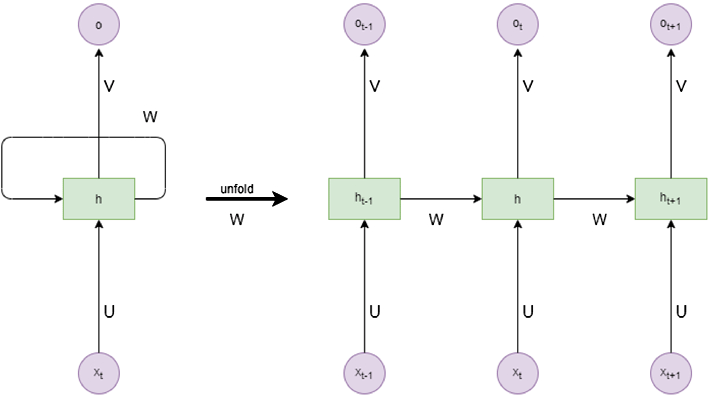
\includegraphics[width=0.9\textwidth]{rnn_unrolled.png}
    \captionof{figure}{Kiến trúc của một RNN. Bên trái là dạng nén với vòng lặp. Bên phải là dạng "trải ra theo thời gian" (unrolled), cho thấy cách trạng thái ẩn $h$ được truyền từ bước này sang bước tiếp theo.}
    \label{fig:rnn_unrolled}
\end{center}

\subsubsection{Kiến trúc và Dòng chảy Dữ liệu}
Tại mỗi bước thời gian $t$:
\begin{enumerate}
    \item \textbf{Đầu vào:} Vector từ $x_t$ và trạng thái ẩn từ bước trước $h_{t-1}$.
    \item \textbf{Tính toán trạng thái ẩn mới:} Trạng thái ẩn mới, $h_t$, được tính bằng cách kết hợp $x_t$ và $h_{t-1}$ qua một phép biến đổi tuyến tính và một hàm kích hoạt (thường là `tanh`).
        \begin{equation}
            h_t = \tanh(W_{hh} h_{t-1} + W_{xh} x_t + b_h)
        \end{equation}
        Trong đó, $W_{hh}$ và $W_{xh}$ là các ma trận trọng số được \textbf{chia sẻ (shared)} trên tất cả các bước thời gian. Đây là điểm mấu chốt: mô hình học một bộ quy tắc duy nhất để cập nhật trí nhớ, bất kể vị trí trong chuỗi.
    \item \textbf{Tạo đầu ra (tùy chọn):} Một đầu ra $y_t$ có thể được tạo ra từ trạng thái ẩn $h_t$.
        \begin{equation}
            y_t = W_{hy} h_t + b_y
        \end{equation}
\end{enumerate}
\begin{tcolorbox}[
    title=Ghi chú sâu về Thiết kế của RNN Đơn giản,
    colback=green!5!white, colframe=green!50!black, fonttitle=\bfseries
]
\textbf{1. Tại sao phải Chia sẻ Trọng số?} \\
Đây là nguyên lý nền tảng của RNN. Việc sử dụng cùng một bộ trọng số ($W_{hh}, W_{xh}$) ở mọi bước thời gian cho phép mô hình học một quy tắc cập nhật \textbf{tổng quát} có thể áp dụng cho bất kỳ vị trí nào trong chuỗi. Nếu mỗi bước thời gian có một bộ trọng số riêng, mô hình sẽ:
\begin{itemize}
    \item Có số lượng tham số khổng lồ, phụ thuộc vào độ dài chuỗi, khiến việc huấn luyện bất khả thi.
    \item Không thể tổng quát hóa cho các chuỗi có độ dài khác với dữ liệu huấn luyện. Nó sẽ chỉ học thuộc lòng các mẫu ở các vị trí cố định.
\end{itemize}
Việc chia sẻ trọng số chính là cách RNN học được một "thuật toán" xử lý chuỗi.

\textbf{2. Tại sao dùng hàm `tanh`?} \\
Hàm `tanh` đưa đầu ra về khoảng $[-1, 1]$. Điều này giúp giữ cho các giá trị trong trạng thái ẩn không bị tăng hoặc giảm quá nhanh, tức là kiểm soát dòng chảy thông tin một cách tương đối ổn định. Nếu dùng `ReLU` (vốn không có giới hạn trên), trạng thái ẩn có thể tăng lên vô hạn, làm cho vấn đề bùng nổ gradient trở nên trầm trọng hơn rất nhiều. `tanh` hoạt động như một cơ chế "bão hòa" tự nhiên.
\end{tcolorbox}

\subsubsection{Huấn luyện RNN: Lan truyền ngược theo thời gian (BPTT)}
\label{sssec:bptt}
Quá trình huấn luyện một RNN cũng dựa trên việc tối thiểu hóa một hàm mất mát, nhưng có một sự phức tạp hơn so với mạng FNN.
\begin{itemize}
    \item \textbf{Hàm Mất mát:} Tại mỗi bước thời gian $t$, mô hình tạo ra một dự đoán $y_t$. Lỗi tại bước đó, $\mathcal{L}_t$, được tính toán bằng cách so sánh $y_t$ với nhãn thật tương ứng. \textbf{Tổng lỗi} cho toàn bộ chuỗi là tổng của các lỗi tại mỗi bước: $\mathcal{L} = \sum_{t=1}^{T} \mathcal{L}_t$.
    
    \item \textbf{Lan truyền ngược theo thời gian (Backpropagation Through Time - BPTT):} Để tính toán gradient của tổng lỗi $\mathcal{L}$ theo các trọng số (ví dụ $W_{hh}$), chúng ta phải sử dụng một biến thể của backpropagation gọi là BPTT. Gradient tại một bước thời gian $t$ không chỉ phụ thuộc vào lỗi tại bước $t$, mà còn phụ thuộc vào gradient từ tất cả các bước thời gian \textit{trong tương lai} ($t+1, t+2, \dots, T$) được truyền ngược lại thông qua trạng thái ẩn $h$.
    
    \item \textbf{Vấn đề của BPTT:} Chính việc gradient phải được truyền ngược qua nhiều bước thời gian này là nguyên nhân gây ra các vấn đề nan giải được thảo luận dưới đây.
\end{itemize}

\subsubsection{Vấn đề nan giải: Vanishing và Exploding Gradients}
RNN về lý thuyết có thể học các phụ thuộc tầm xa. Tuy nhiên, trong thực tế, chúng gặp rất nhiều khó khăn. Quá trình huấn luyện RNN sử dụng thuật toán lan truyền ngược theo thời gian (Backpropagation Through Time - BPTT). Khi lan truyền gradient lỗi ngược qua nhiều bước thời gian, gradient này phải đi qua phép nhân lặp đi lặp lại với ma trận trọng số $W_{hh}$.

\begin{itemize}
    \item \textbf{Vanishing Gradients (Triệt tiêu Gradient):} Nếu các giá trị trong $W_{hh}$ nhỏ (norm < 1), sau nhiều lần nhân, gradient sẽ co lại và tiến dần về 0.
        \begin{itemize}
            \item \textbf{Hậu quả:} Mạng không thể học được các phụ thuộc giữa các từ ở xa nhau. Tín hiệu lỗi từ tương lai không thể lan truyền đủ xa về quá khứ để cập nhật trọng số một cách có ý nghĩa. RNN trở nên "thiển cận", chỉ nhớ được vài bước gần nhất. Đây là vấn đề nghiêm trọng nhất.
        \end{itemize}
    \item \textbf{Exploding Gradients (Bùng nổ Gradient):} Nếu các giá trị trong $W_{hh}$ lớn (norm > 1), gradient sẽ tăng theo cấp số nhân và trở nên khổng lồ.
        \begin{itemize}
            \item \textbf{Hậu quả:} Gây ra các bước cập nhật trọng số cực lớn, làm cho quá trình huấn luyện trở nên mất ổn định. Vấn đề này có thể được giải quyết phần nào bằng kỹ thuật \textit{gradient clipping} (cắt bớt gradient nếu nó vượt quá một ngưỡng).
        \end{itemize}
\end{itemize}

Vấn đề triệt tiêu gradient đã thúc đẩy sự ra đời của các kiến trúc RNN phức tạp hơn, có khả năng kiểm soát dòng chảy thông tin một cách thông minh hơn.

\subsection{Long Short-Term Memory (LSTM)}
\label{ssec:lstm}
LSTM, được giới thiệu bởi Hochreiter \& Schmidhuber vào năm 1997 \cite{hochreiter1997long}, là một biến thể đặc biệt của RNN, được thiết kế một cách xuất sắc để giải quyết vấn đề triệt tiêu gradient. Nó đã trở thành kiến trúc thống trị cho các bài toán chuỗi trong gần hai thập kỷ.

\subsubsection{Tư duy cốt lõi: Các Cổng và Trạng thái Ô nhớ}
Ý tưởng thiên tài của LSTM là giới thiệu một "làn đường cao tốc" cho thông tin, gọi là \textbf{trạng thái ô nhớ (cell state)}, ký hiệu là $C_t$. Trạng thái ô nhớ này chạy dọc theo toàn bộ chuỗi, chỉ với một vài tương tác tuyến tính nhỏ. Thông tin có thể dễ dàng chảy trên làn đường này mà không bị thay đổi nhiều.

LSTM có khả năng thêm hoặc bớt thông tin ra khỏi trạng thái ô nhớ một cách cẩn thận, được điều khiển bởi các cấu trúc gọi là \textbf{cổng (gates)}. Cổng là một cách để thông tin có thể đi qua một cách tùy chọn. Chúng bao gồm một lớp mạng sigmoid và một phép nhân theo từng phần tử (element-wise multiplication).

\begin{center}
    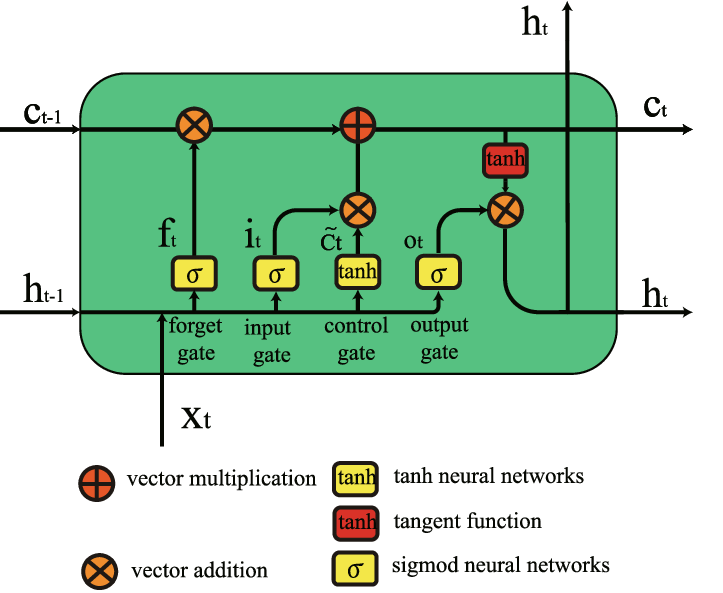
\includegraphics[width=0.7\textwidth]{lstm_cell_diagram.png}
    \captionof{figure}{Sơ đồ chi tiết của một ô nhớ LSTM. Nó bao gồm 3 cổng chính (Quên, Nạp, Xuất) và một trạng thái ô nhớ $C_t$ chạy ngang.}
    \label{fig:lstm_cell_diagram}
\end{center}

Một ô LSTM có ba cổng để bảo vệ và kiểm soát trạng thái ô nhớ:

\paragraph{1. Cổng Quên (Forget Gate - $f_t$)}
Cổng này quyết định xem thông tin nào nên được \textbf{loại bỏ} khỏi trạng thái ô nhớ của bước trước.
$$ f_t = \sigma(W_f [h_{t-1}, x_t] + b_f) $$
Nó nhìn vào $h_{t-1}$ và $x_t$, và xuất ra một vector số từ 0 đến 1 cho mỗi số trong trạng thái ô nhớ $C_{t-1}$. Số 1 có nghĩa là "giữ lại hoàn toàn", số 0 có nghĩa là "quên hoàn toàn".

\paragraph{2. Cổng Nạp (Input Gate - $i_t$)}
Cổng này quyết định xem thông tin mới nào nên được \textbf{lưu trữ} vào trạng thái ô nhớ. Quá trình này có hai bước:
\begin{enumerate}
    \item Một lớp sigmoid (cổng nạp) quyết định những giá trị nào chúng ta sẽ cập nhật.
        $$ i_t = \sigma(W_i [h_{t-1}, x_t] + b_i) $$
    \item Một lớp `tanh` tạo ra một vector các giá trị ứng viên mới, $\tilde{C}_t$, có thể được thêm vào trạng thái.
        $$ \tilde{C}_t = \tanh(W_C [h_{t-1}, x_t] + b_C) $$
\end{enumerate}

\paragraph{3. Cập nhật Trạng thái Ô nhớ}
Bây giờ, chúng ta cập nhật trạng thái ô nhớ cũ $C_{t-1}$ thành trạng thái mới $C_t$.
$$ C_t = f_t \odot C_{t-1} + i_t \odot \tilde{C}_t $$
Ký hiệu $\odot$ là phép nhân theo từng phần tử. Chúng ta nhân trạng thái cũ với $f_t$ (quên đi những gì đã quyết định quên), sau đó cộng với $i_t \odot \tilde{C}_t$ (thêm vào những thông tin mới đã quyết định nạp). Phép cộng này chính là chìa khóa giúp gradient có thể chảy ngược một cách dễ dàng, giải quyết vấn đề triệt tiêu gradient.

\paragraph{4. Cổng Xuất (Output Gate - $o_t$)}
Cuối cùng, cổng này quyết định xem chúng ta sẽ xuất ra cái gì. Đầu ra này sẽ dựa trên trạng thái ô nhớ của chúng ta, nhưng sẽ là một phiên bản đã được "lọc".
\begin{enumerate}
    \item Một lớp sigmoid quyết định phần nào của trạng thái ô nhớ chúng ta sẽ xuất ra.
        $$ o_t = \sigma(W_o [h_{t-1}, x_t] + b_o) $$
    \item Chúng ta đưa trạng thái ô nhớ qua hàm `tanh` (để đưa giá trị về khoảng [-1, 1]) và nhân nó với đầu ra của cổng sigmoid, để chỉ xuất ra những phần chúng ta muốn.
        $$ h_t = o_t \odot \tanh(C_t) $$
\end{enumerate}
Trạng thái ẩn mới $h_t$ này sẽ được sử dụng để dự đoán đầu ra $y_t$ và được truyền tới bước thời gian tiếp theo.
\paragraph{Phân tích: Tại sao LSTM hoạt động?}
Sự kỳ diệu của LSTM nằm ở cách nó tách biệt dòng chảy thông tin và kiểm soát nó một cách tinh vi:
\begin{itemize}
    \item \textbf{Con đường cao tốc Gradient (Gradient Highway):} Nhìn lại công thức cập nhật trạng thái ô nhớ: $C_t = f_t \odot C_{t-1} + i_t \odot \tilde{C}_t$. Thành phần quan trọng nhất là phép cộng. Trong quá trình lan truyền ngược, gradient của $C_t$ đối với $C_{t-1}$ có một thành phần trực tiếp là $f_t$. Do $f_t$ được điều khiển bởi hàm sigmoid, giá trị của nó thường không bị quá nhỏ hoặc quá lớn. Điều này tạo ra một "con đường" gần như không bị cản trở để gradient có thể chảy ngược qua nhiều bước thời gian mà không bị triệt tiêu hoàn toàn. RNN đơn giản chỉ có phép nhân lặp đi lặp lại, khiến gradient dễ dàng biến mất.
    
    \item \textbf{Phân vai Trí nhớ:} LSTM tạo ra một sự phân vai rõ ràng:
        \begin{itemize}
            \item \textbf{Trạng thái Ô nhớ ($C_t$):} Đóng vai trò như \textbf{trí nhớ dài hạn}. Nó chứa tất cả thông tin tích lũy được. Nó có thể được thay đổi một cách cẩn trọng thông qua các cổng, nhưng bản chất là một "kho lưu trữ".
            \item \textbf{Trạng thái Ẩn ($h_t$):} Đóng vai trò như \textbf{trí nhớ làm việc (working memory)}. Nó là một phiên bản "đã lọc" của trí nhớ dài hạn, chỉ chứa những thông tin liên quan đến quyết định cần đưa ra \textit{tại thời điểm hiện tại}. Việc tách biệt này cho phép mô hình vừa lưu trữ thông tin từ rất xa trong quá khứ ($C_t$), vừa tập trung vào những gì cần thiết cho bước tiếp theo ($h_t$).
        \end{itemize}
\end{itemize}
\subsection{Gated Recurrent Unit (GRU)}
\label{ssec:gru}
Được giới thiệu bởi Cho và các cộng sự vào năm 2014, GRU \cite{cho2014learning} là một biến thể của LSTM với kiến trúc đơn giản hơn. Nó kết hợp cổng quên và cổng nạp thành một "cổng cập nhật" duy nhất, và cũng hợp nhất trạng thái ô nhớ và trạng thái ẩn.

\paragraph{Tư duy cốt lõi}
GRU giữ lại tinh thần của LSTM là sử dụng các cổng để điều khiển dòng chảy thông tin, nhưng với ít tham số hơn, giúp việc huấn luyện nhanh hơn và hiệu quả hơn trên các bộ dữ liệu nhỏ.

GRU có hai cổng chính:
\paragraph{1. Cổng Cập nhật (Update Gate - $z_t$)}
Cổng này có vai trò tương tự cả cổng quên và cổng nạp trong LSTM. Nó quyết định xem bao nhiêu thông tin từ trạng thái ẩn quá khứ ($h_{t-1}$) nên được giữ lại, và bao nhiêu thông tin mới ($\tilde{h}_t$) nên được thêm vào.
$$ z_t = \sigma(W_z [h_{t-1}, x_t] + b_z) $$

\paragraph{2. Cổng Reset (Reset Gate - $r_t$)}
Cổng này quyết định xem bao nhiêu phần của trạng thái ẩn quá khứ nên được "quên" đi khi tính toán trạng thái ứng viên mới.
$$ r_t = \sigma(W_r [h_{t-1}, x_t] + b_r) $$

\paragraph{Tính toán Trạng thái}
\begin{enumerate}
    \item Trạng thái ẩn ứng viên mới $\tilde{h}_t$ được tính toán, nhưng có sử dụng cổng reset để kiểm soát ảnh hưởng của $h_{t-1}$.
        $$ \tilde{h}_t = \tanh(W_h [r_t \odot h_{t-1}, x_t] + b_h) $$
        Nếu cổng reset $r_t$ gần bằng 0, mô hình sẽ gần như bỏ qua hoàn toàn thông tin quá khứ và chỉ tập trung vào đầu vào hiện tại $x_t$ để tạo trạng thái mới.
    \item Trạng thái ẩn cuối cùng $h_t$ là một sự nội suy tuyến tính giữa trạng thái cũ $h_{t-1}$ và trạng thái ứng viên mới $\tilde{h}_t$, được điều khiển bởi cổng cập nhật $z_t$.
        $$ h_t = (1 - z_t) \odot h_{t-1} + z_t \odot \tilde{h}_t $$
\end{enumerate}
\paragraph{Phân tích: Sự đánh đổi của GRU}
GRU là một ví dụ tuyệt vời về việc đơn giản hóa kiến trúc mà vẫn giữ được hiệu quả cốt lõi.
\begin{itemize}
    \item \textbf{Cổng Reset - Cơ chế "Khởi động lại Ngữ cảnh":} Cổng reset ($r_t$) cho phép GRU bỏ qua hoàn toàn trí nhớ quá khứ khi cần thiết. Hãy tưởng tượng khi đọc một đoạn văn và gặp một dấu chấm hết câu, bắt đầu một câu mới với chủ đề khác. Cổng reset có thể học cách "kích hoạt" (đưa giá trị về gần 0) tại những điểm chuyển tiếp này, cho phép trạng thái ứng viên mới $\tilde{h}_t$ được hình thành chủ yếu từ đầu vào hiện tại $x_t$, tạo ra một khởi đầu mới cho ngữ cảnh.
    
    \item \textbf{Cổng Cập nhật - Nội suy mượt mà:} Công thức $h_t = (1 - z_t) \odot h_{t-1} + z_t \odot \tilde{h}_t$ hoạt động như một bộ điều khiển "rò rỉ". Khi $z_t$ gần bằng 0, phần lớn $h_{t-1}$ sẽ được sao chép trực tiếp sang $h_t$, giúp thông tin được bảo tồn qua các bước thời gian dài. Ngược lại, khi $z_t$ gần bằng 1, thông tin mới sẽ được ưu tiên. Sự cân bằng này giúp GRU mô hình hóa các phụ thuộc dài hạn một cách hiệu quả, dù không có một "trạng thái ô nhớ" riêng biệt.
\end{itemize}
Việc gộp trạng thái ô nhớ và trạng thái ẩn làm cho GRU mất đi một chút sức mạnh biểu diễn so với LSTM, nhưng chính sự đơn giản này lại giúp nó huấn luyện nhanh hơn và đôi khi tổng quát hóa tốt hơn trên các tập dữ liệu nhỏ.
\begin{tcolorbox}[
    title=So sánh LSTM và GRU,
    colback=green!5!white, colframe=green!60!black, fonttitle=\bfseries
]
\begin{tabular}{p{0.45\linewidth} | p{0.45\linewidth}}
    \textbf{LSTM} & \textbf{GRU} \\
    \hline
    Có 3 cổng: Quên, Nạp, Xuất. & Có 2 cổng: Cập nhật, Reset. \\
    \hline
    Có trạng thái ô nhớ ($C_t$) và trạng thái ẩn ($h_t$) riêng biệt. & Chỉ có một trạng thái ẩn ($h_t$). \\
    \hline
    Nhiều tham số hơn. & Ít tham số hơn. \\
    \hline
    Linh hoạt và mạnh mẽ hơn về mặt lý thuyết. & Nhanh hơn, hiệu quả hơn về mặt tính toán và cần ít dữ liệu hơn để tổng quát hóa. \\
    \hline
    \textbf{Khi nào dùng?} Không có quy tắc tuyệt đối. GRU là một lựa chọn khởi đầu tốt. Nếu bài toán rất phức tạp và có đủ dữ liệu, LSTM có thể cho hiệu năng nhỉnh hơn.
\end{tabular}
\end{tcolorbox}
% % !TEX root = ../main.tex
% File: chapters_part1/chap3_4.tex
% Nội dung cho Phần 3.4: Seq2Seq và Attention

\section{Mô hình Chuỗi-sang-Chuỗi (Seq2Seq) và Cơ chế Chú ý (Attention)}
\label{sec:seq2seq_attention}

Kiến trúc RNN, LSTM, hay GRU mà chúng ta vừa học có một hạn chế cơ bản: chúng được thiết kế để xử lý các bài toán có đầu vào là một chuỗi và đầu ra là một giá trị duy nhất (phân loại) hoặc một chuỗi có độ dài bằng với chuỗi đầu vào (gán nhãn chuỗi).

Nhưng điều gì sẽ xảy ra với các bài toán như \textbf{dịch máy} (một câu tiếng Việt có 10 từ có thể được dịch thành một câu tiếng Anh 8 từ) hoặc \textbf{tóm tắt văn bản} (một văn bản 1000 từ được tóm tắt thành một câu 20 từ)? Ở những bài toán này, độ dài chuỗi đầu vào và đầu ra là khác nhau và không có sự tương ứng 1-1.

Mô hình Chuỗi-sang-Chuỗi (Sequence-to-Sequence - Seq2Seq) ra đời để giải quyết chính xác vấn đề này.

\subsection{Kiến trúc Encoder-Decoder của Seq2Seq}
\label{ssec:encoder_decoder}
Seq2Seq, được giới thiệu gần như đồng thời bởi Sutskever và các cộng sự (2014) \cite{sutskever2014sequence} và Cho và các cộng sự (2014) \cite{cho2014learning}, dựa trên một kiến trúc thanh lịch gồm hai thành phần chính: \textbf{Bộ mã hóa (Encoder)} và \textbf{Bộ giải mã (Decoder)}.

\begin{center}
    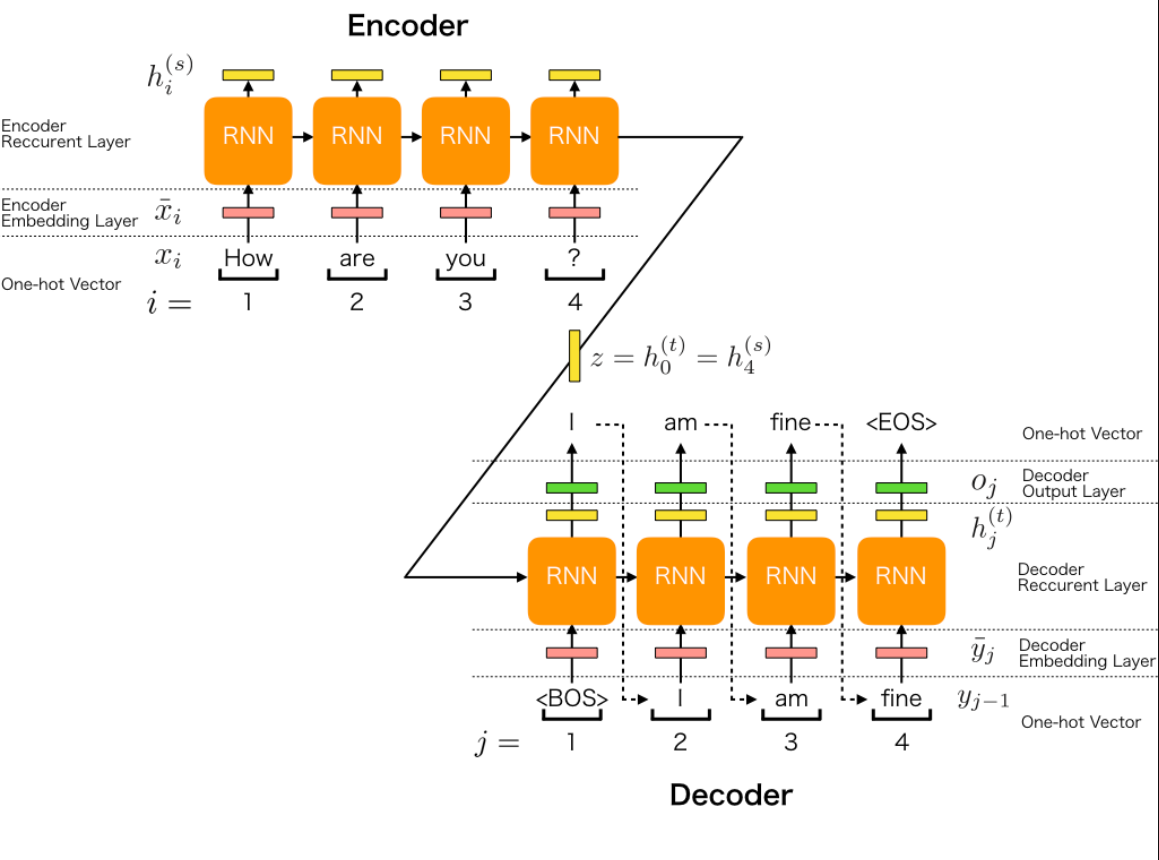
\includegraphics[width=0.9\textwidth]{seq2seq_architecture.png}
    \captionof{figure}{Kiến trúc Encoder-Decoder tổng quát. Encoder "đọc" và nén chuỗi đầu vào thành một vector ngữ cảnh. Decoder sử dụng vector này để "viết" ra chuỗi đầu ra.}
    \label{fig:seq2seq_architecture}
\end{center}

\subsubsection{Bộ mã hóa (The Encoder)}
\paragraph{Nhiệm vụ}
Nhiệm vụ của Encoder là "đọc" toàn bộ chuỗi đầu vào (ví dụ, một câu tiếng Việt) và nén toàn bộ thông tin, ngữ nghĩa của nó vào một vector có kích thước cố định. Vector này được gọi là \textbf{vector ngữ cảnh (context vector)} hay "thought vector".

\paragraph{Cấu tạo và Hoạt động}
\begin{itemize}
    \item Encoder thường là một mạng RNN (hoặc LSTM, GRU).
    \item Nó nhận đầu vào là một chuỗi các vector từ (word embeddings) của câu nguồn, ví dụ: $x_1, x_2, \dots, x_T$.
    \item Nó xử lý chuỗi này tuần tự, từng từ một. Tại mỗi bước, nó cập nhật trạng thái ẩn của mình.
    \item Điều quan trọng là chúng ta \textbf{bỏ qua tất cả các đầu ra (outputs) của Encoder ở mỗi bước}. Chúng ta chỉ quan tâm đến \textbf{trạng thái ẩn cuối cùng ($h_T$)}. Trạng thái ẩn cuối cùng này chính là vector ngữ cảnh, vì nó được cho là đã tóm tắt thông tin của toàn bộ chuỗi đầu vào.
\end{itemize}
\begin{tcolorbox}[
    title=Ghi chú sâu về Thiết kế của Encoder,
    colback=green!5!white, colframe=green!50!black, fonttitle=\bfseries
]
\textbf{1. Tại sao Encoder thường là Mạng RNN Hai chiều (Bi-RNN)?} \\
Một RNN đơn giản xử lý câu từ trái sang phải. Trạng thái ẩn $h_t$ tại từ $x_t$ chỉ chứa thông tin về các từ từ $x_1$ đến $x_t$. Điều này là một hạn chế, vì ngữ nghĩa của một từ thường phụ thuộc vào cả ngữ cảnh đứng trước và đứng sau nó.
\begin{itemize}
    \item \textbf{Bi-RNN} giải quyết vấn đề này bằng cách sử dụng hai RNN riêng biệt: một RNN chạy xuôi (forward) từ đầu đến cuối câu, và một RNN chạy ngược (backward) từ cuối về đầu.
    \item Tại mỗi từ $x_t$, biểu diễn cuối cùng của nó là sự \textbf{kết hợp} (thường là nối - concatenation) của trạng thái ẩn từ cả hai chiều: $\overrightarrow{h_t}$ và $\overleftarrow{h_t}$.
    \item Vector ngữ cảnh cuối cùng cho mô hình Seq2Seq cơ bản sẽ là nối của trạng thái ẩn cuối cùng của RNN xuôi ($\overrightarrow{h_T}$) và trạng thái ẩn cuối cùng của RNN ngược ($\overleftarrow{h_1}$).
\end{itemize}
Việc này cung cấp một biểu diễn ngữ cảnh phong phú hơn nhiều cho mỗi từ, và đã trở thành tiêu chuẩn trong hầu hết các mô hình Encoder-Decoder.

\textbf{2. Tại sao không dùng Pooling thay vì trạng thái ẩn cuối cùng?} \\
Sử dụng trạng thái ẩn cuối cùng là cách đơn giản nhất, nhưng nó có thể bị ảnh hưởng bởi "hiệu ứng gần đây" (recency bias) - các từ cuối chuỗi có thể có ảnh hưởng lớn hơn. Các phương pháp khác như:
\begin{itemize}
    \item \textbf{Average/Max Pooling:} Lấy trung bình hoặc giá trị lớn nhất trên tất cả các trạng thái ẩn (của Bi-RNN). Cách này dân chủ hơn, đảm bảo mọi từ đều có đóng góp, nhưng có thể làm "lu mờ" các chi tiết quan trọng.
\end{itemize}
Trong thực tế, trước khi Attention ra đời, không có phương pháp nào là hoàn hảo. Sự ra đời của Attention đã giải quyết triệt để vấn đề này bằng cách cho phép Decoder tự quyết định nên tập trung vào đâu, thay vì ép Encoder phải tạo ra một bản tóm tắt duy nhất.
\end{tcolorbox}
\subsubsection{Bộ giải mã (The Decoder)}
\paragraph{Nhiệm vụ}
Nhiệm vụ của Decoder là lấy vector ngữ cảnh do Encoder cung cấp và "giải nén" nó để sinh ra chuỗi đầu ra (ví dụ, câu tiếng Anh tương ứng), từng từ một.

\paragraph{Cấu tạo và Hoạt động}
\begin{itemize}
    \item Decoder cũng là một mạng RNN (hoặc LSTM, GRU) khác, thường có kiến trúc tương tự Encoder nhưng với bộ trọng số riêng.
    \item \textbf{Khởi tạo:} Trạng thái ẩn ban đầu của Decoder ($h_0^{dec}$) được khởi tạo bằng chính vector ngữ cảnh (trạng thái ẩn cuối cùng của Encoder, $h_T^{enc}$). Đây là "cây cầu" duy nhất kết nối Encoder và Decoder.
    \item \textbf{Quá trình sinh từ (Generation):} Quá trình này diễn ra tuần tự:
        \begin{enumerate}
            \item \textbf{Bước 1:} Decoder nhận vào một token bắt đầu đặc biệt (ví dụ: `<SOS>` - Start of Sentence) và trạng thái ẩn ban đầu. Nó tính toán trạng thái ẩn mới $h_1^{dec}$ và tạo ra một phân phối xác suất trên toàn bộ từ vựng của ngôn ngữ đích thông qua một lớp softmax. Từ có xác suất cao nhất được chọn làm từ đầu ra đầu tiên, $y_1$.
            \item \textbf{Bước 2:} Từ vừa được sinh ra, $y_1$, sẽ trở thành \textbf{đầu vào cho bước tiếp theo}. Decoder nhận $y_1$ và trạng thái ẩn $h_1^{dec}$ để tính $h_2^{dec}$ và sinh ra từ tiếp theo $y_2$.
            \item Quá trình này lặp đi lặp lại (mang tính \textbf{tự hồi quy - auto-regressive}) cho đến khi Decoder sinh ra một token kết thúc đặc biệt (`<EOS>` - End of Sentence).
        \end{enumerate}
\end{itemize}

\subsubsection{Vấn đề của cái "Cổ chai" (The Bottleneck Problem)}
Kiến trúc Encoder-Decoder cơ bản này rất thông minh, nhưng nó có một điểm yếu chết người: nó buộc Encoder phải nén toàn bộ thông tin của một câu, dù dài và phức tạp đến đâu, vào một \textbf{vector ngữ cảnh có kích thước cố định}.
\begin{itemize}
    \item Đây là một "cổ chai" thông tin. Với những câu dài, việc nhồi nhét tất cả các chi tiết ngữ nghĩa vào một vector duy nhất là cực kỳ khó khăn, nếu không muốn nói là bất khả thi.
    \item Decoder chỉ được "nhìn" vào bản tóm tắt này một lần duy nhất lúc bắt đầu. Nó không có cách nào để quay lại và xem xét các phần cụ thể của câu nguồn khi nó đang dịch.
\end{itemize}
Hãy tưởng tượng bạn yêu cầu một dịch giả nghe toàn bộ một bài phát biểu dài, sau đó phải dịch lại toàn bộ từ trí nhớ mà không được ghi chép. Đó chính là những gì mô hình Seq2Seq cơ bản phải làm. Hạn chế này đã dẫn đến sự ra đời của ý tưởng có sức ảnh hưởng bậc nhất trong lịch sử NLP hiện đại: \textbf{Cơ chế Chú ý (Attention)}.

\subsubsection{Huấn luyện mô hình Seq2Seq}
Mục tiêu huấn luyện của mô hình Seq2Seq là tối đa hóa xác suất của chuỗi đầu ra đúng ($Y = y_1, ..., y_{T'}$) khi biết chuỗi đầu vào ($X = x_1, ..., x_T$). Điều này tương đương với việc tối thiểu hóa hàm mất mát \textbf{Cross-Entropy} trên toàn bộ chuỗi đầu ra:
$$ \mathcal{L}(\theta) = - \sum_{t=1}^{T'} \log P(y_t | y_1, ..., y_{t-1}, c) $$
trong đó $c$ là vector ngữ cảnh từ Encoder. Trong quá trình huấn luyện, lỗi tại mỗi bước của Decoder được tính toán và lan truyền ngược qua cả Decoder và Encoder để cập nhật tất cả các trọng số. Kỹ thuật \textbf{Teacher Forcing} được sử dụng để làm cho quá trình này ổn định và hiệu quả hơn.

\subsubsection{Huấn luyện và Suy luận: Teacher Forcing và Beam Search}
Có hai kỹ thuật quan trọng liên quan đến cách mô hình Seq2Seq được huấn luyện và sử dụng để sinh văn bản.

\paragraph{Huấn luyện với Teacher Forcing}
Trong quá trình huấn luyện, tại mỗi bước $t$, thay vì đưa từ mà Decoder vừa dự đoán ở bước $t-1$ vào làm đầu vào, chúng ta lại đưa từ \textbf{chính xác (ground truth)} trong chuỗi đích vào.
\begin{itemize}
    \item \textbf{Ưu điểm:} Kỹ thuật này giúp quá trình huấn luyện ổn định và hội tụ nhanh hơn rất nhiều. Nó ngăn ngừa việc lỗi bị tích tụ: nếu mô hình dự đoán sai ở bước đầu, lỗi sai đó sẽ không làm ảnh hưởng đến các bước sau trong cùng một chuỗi huấn luyện. Mỗi bước thời gian được coi là một mẫu huấn luyện độc lập.
    \item \textbf{Nhược điểm:} Nó tạo ra một sự khác biệt giữa lúc huấn luyện và lúc suy luận (khi mô hình không có "thầy" để chỉ bảo). Điều này có thể dẫn đến hiệu năng kém khi mô hình phải tự sinh ra một chuỗi dài.
\end{itemize}

\paragraph{Suy luận với Beam Search}
Trong lúc suy luận, việc luôn chọn từ có xác suất cao nhất tại mỗi bước (gọi là \textbf{Greedy Search}) thường không tạo ra được câu tốt nhất. Một lựa chọn có vẻ tốt ở hiện tại có thể dẫn đến một ngõ cụt. \textbf{Beam Search} là một giải pháp cân bằng.
\begin{itemize}
    \item Thay vì chỉ giữ lại 1 ứng viên tốt nhất ở mỗi bước, Beam Search sẽ giữ lại $k$ ứng viên (gọi là \textit{beam width} hoặc \textit{kích thước beam}) có xác suất chuỗi cao nhất.
    \item Tại bước tiếp theo, nó sẽ mở rộng mỗi ứng viên trong beam với tất cả các từ khả dĩ trong từ vựng, tính toán xác suất của các chuỗi mới, và lại chọn ra $k$ chuỗi tốt nhất để tiếp tục.
    \item Quá trình này là một sự đánh đổi giữa chất lượng và chi phí tính toán. Nó hiệu quả hơn nhiều so với Greedy Search và là kỹ thuật tiêu chuẩn để sinh văn bản trong các mô hình Seq2Seq.
\end{itemize}
\subsection{Cơ chế Chú ý (Attention Mechanism)}
\label{ssec:attention}

\subsubsection{Trực giác cốt lõi: Dịch như con người}
Khi một dịch giả con người dịch một câu, họ không làm như mô hình Seq2Seq cơ bản. Khi dịch một từ, họ sẽ tập trung (pay attention) vào một hoặc một vài từ liên quan trong câu gốc. Cơ chế Chú ý được thiết kế để mô phỏng chính xác hành vi này.

\begin{tcolorbox}[
    title=Ý tưởng đột phá của Attention,
    colback=yellow!10!white, colframe=yellow!50!black, fonttitle=\bfseries
]
Thay vì ép Encoder tạo ra một vector ngữ cảnh duy nhất, hãy cho phép Decoder, tại \textbf{mỗi bước} sinh từ của mình, có khả năng \textbf{"nhìn lại" toàn bộ chuỗi đầu vào} và quyết định xem phần nào của chuỗi đầu vào là quan trọng nhất cần phải "chú ý" đến ngay tại thời điểm đó.
\end{tcolorbox}

Attention tạo ra một "đường tắt" kết nối trực tiếp Decoder với tất cả các trạng thái ẩn của Encoder, phá vỡ cái "cổ chai" thông tin.

\subsubsection{Cơ chế hoạt động chi tiết}
Cơ chế chú ý được tích hợp vào giữa Encoder và Decoder. Thay vì chỉ truyền trạng thái ẩn cuối cùng, Encoder sẽ cung cấp \textbf{tất cả các trạng thái ẩn của nó} ($h_1^{enc}, h_2^{enc}, \dots, h_T^{enc}$) cho Decoder.

Bây giờ, tại mỗi bước $t$ của Decoder, để sinh ra từ $y_t$, nó sẽ thực hiện các bước sau:

\begin{center}
    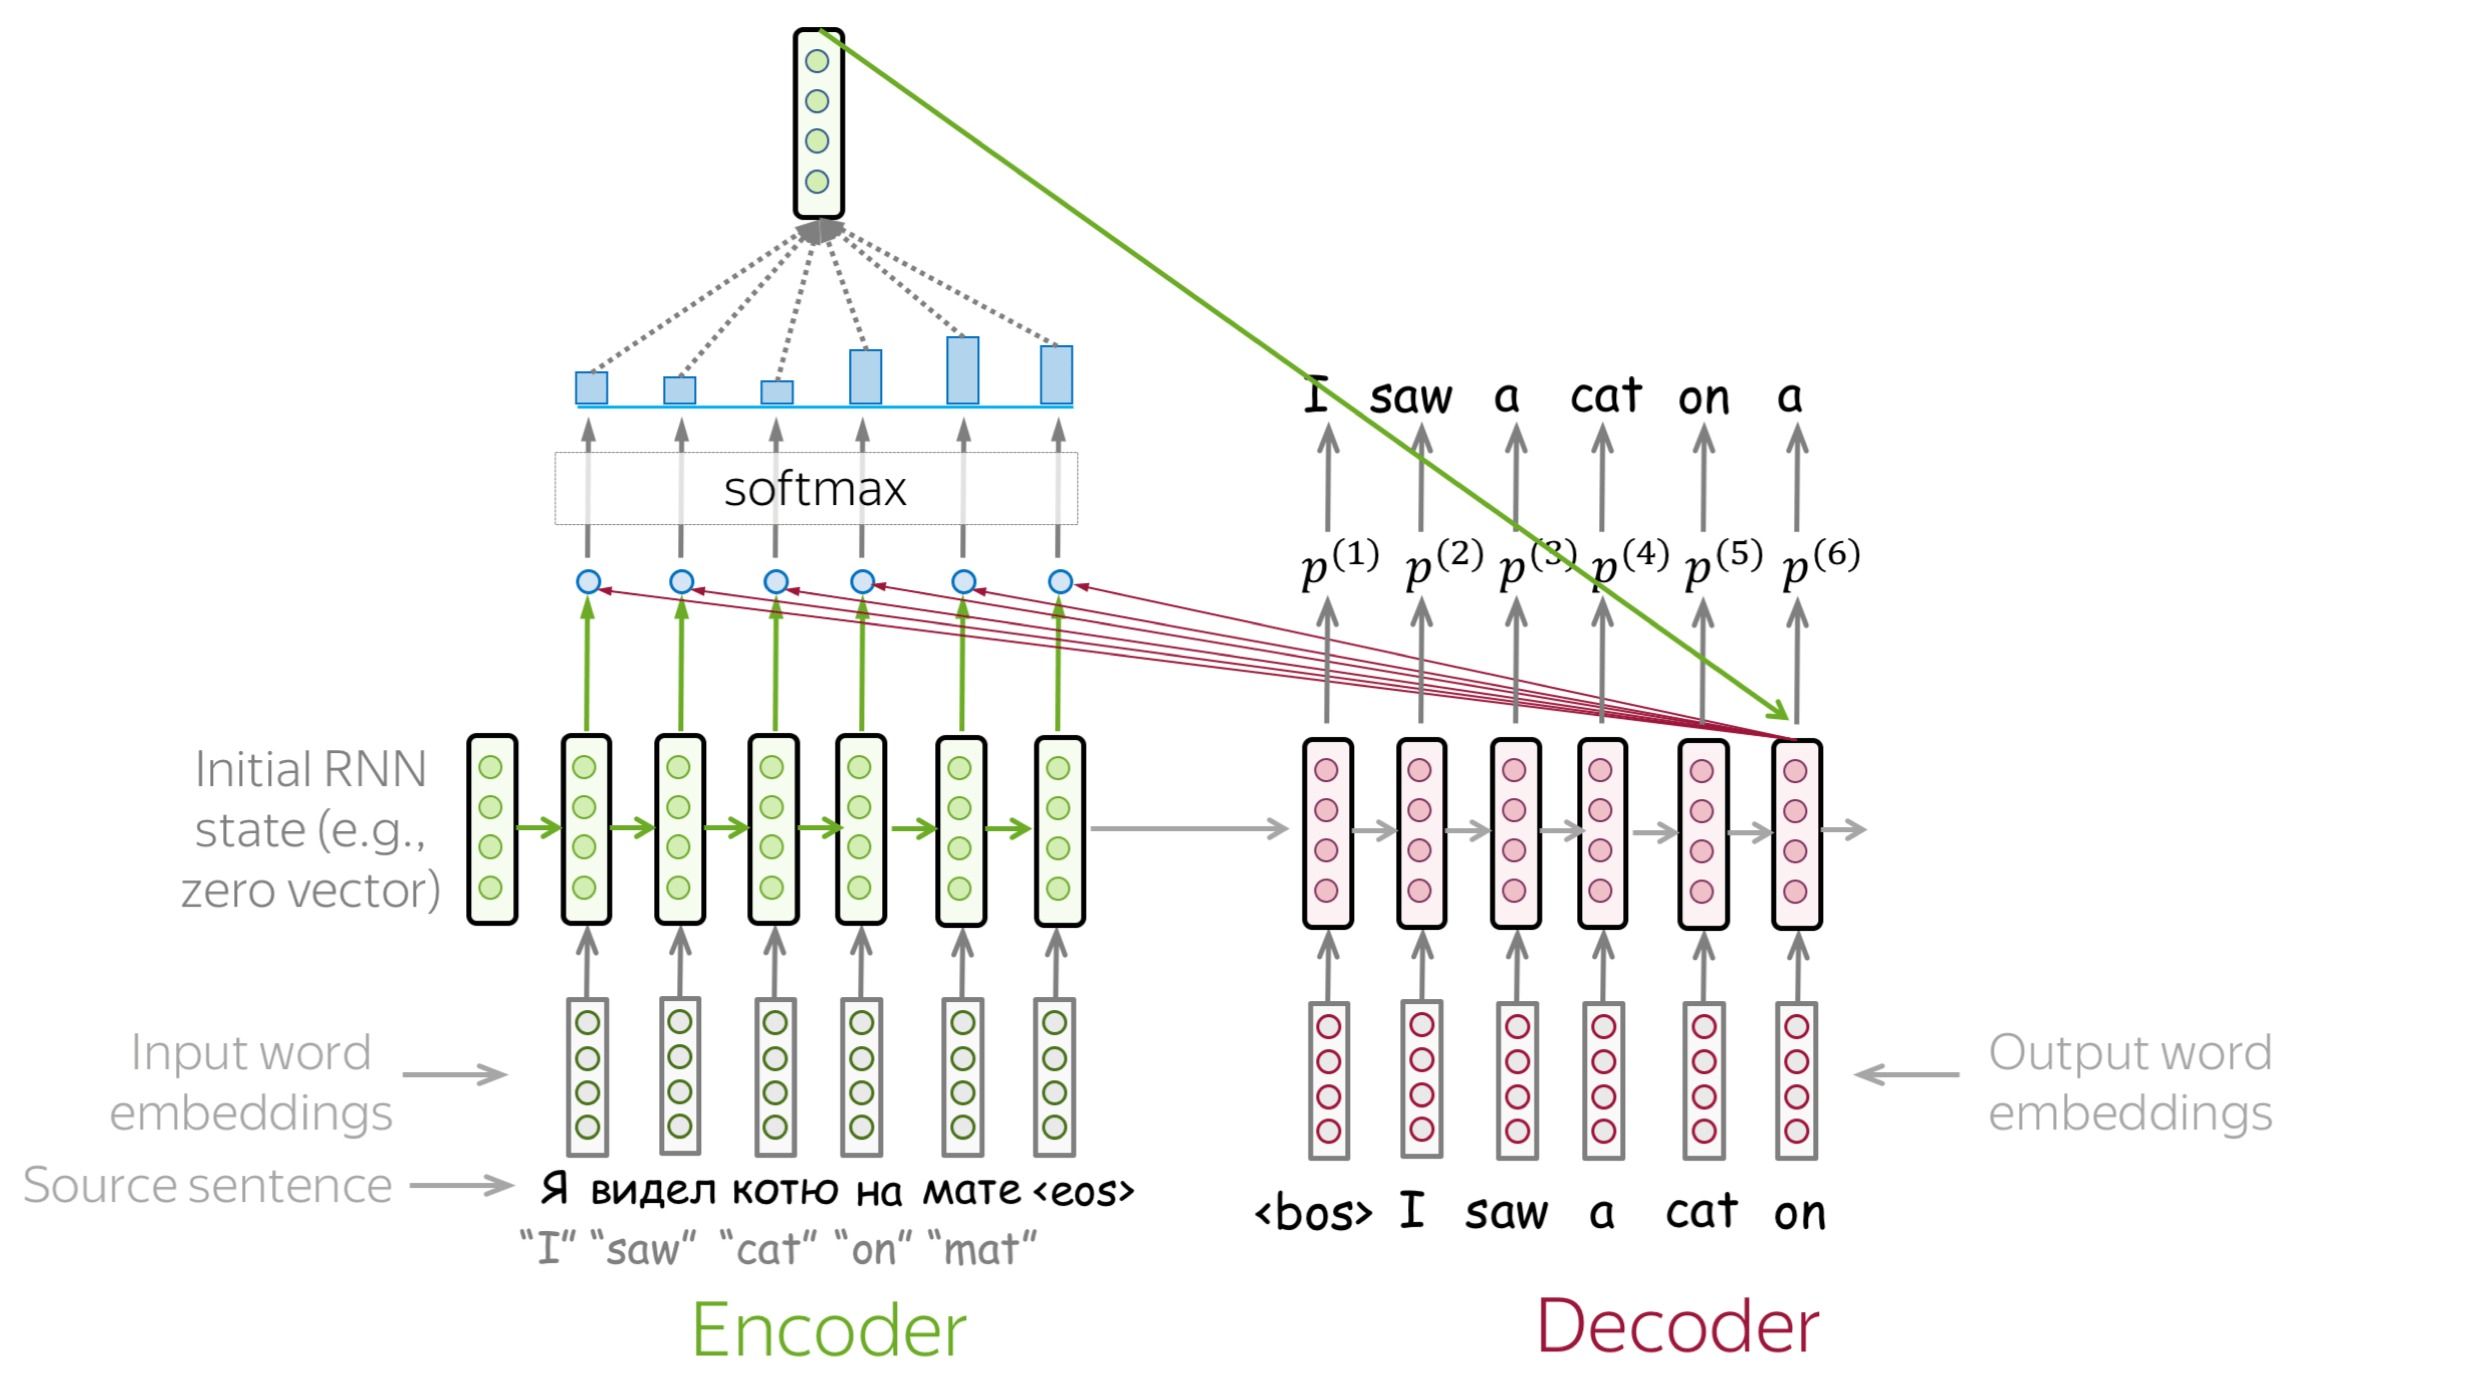
\includegraphics[width=1.0\textwidth]{seq2seq_attention_mechanism.png}
    \captionof{figure}{Cơ chế Chú ý trong Seq2Seq. Tại bước sinh từ thứ $t$ của Decoder, nó tính toán các trọng số chú ý ($\alpha_t$) để tạo ra một vector ngữ cảnh động ($c_t$) từ tất cả các trạng thái ẩn của Encoder.}
    \label{fig:seq2seq_attention_mechanism}
\end{center}

\paragraph{Bước 1: Tính điểm chú ý (Attention Scores)}
Decoder lấy trạng thái ẩn của nó ở bước trước, $h_{t-1}^{dec}$, và so sánh nó với \textbf{từng trạng thái ẩn của Encoder}, $h_i^{enc}$, để tính ra một "điểm số tương hợp" (alignment score). Điểm số này đo lường mức độ "liên quan" của từ đầu vào thứ $i$ đối với việc sinh ra từ đầu ra thứ $t$. Có nhiều cách để định nghĩa hàm $\text{score}(h_{t-1}^{dec}, h_i^{enc})$, trong đó phổ biến là:
\begin{itemize}
    \item \textbf{Additive Attention (\cite{bahdanau2014neural}):} Sử dụng một mạng nơ-ron nhỏ truyền thẳng (feed-forward) có một lớp ẩn. Cách này mạnh mẽ và linh hoạt.
        $$ \text{score}(h_{t-1}^{dec}, h_i^{enc}) = v_a^T \tanh(W_a [h_{t-1}^{dec}; h_i^{enc}]) $$
    \item \textbf{Dot-Product Attention (\cite{luong2015effective}):} Đơn giản là lấy tích vô hướng giữa hai vector. Cách này rất nhanh và hiệu quả về mặt tính toán, nhưng yêu cầu số chiều của $h^{dec}$ và $h^{enc}$ phải bằng nhau.
        $$ \text{score}(h_{t-1}^{dec}, h_i^{enc}) = (h_{t-1}^{dec})^T h_i^{enc} $$
    \item \textbf{Scaled Dot-Product Attention:} Một biến thể của Dot-Product, được giới thiệu trong bài báo Transformer \cite{vaswani2017attention}. Nó chia tích vô hướng cho căn bậc hai của số chiều vector ($\sqrt{d_k}$) để tránh gradient quá nhỏ khi số chiều lớn.
\end{itemize}
Sự lựa chọn hàm score ảnh hưởng đến độ phức tạp tính toán và hiệu năng của mô hình. Dot-Product và các biến thể của nó đã trở nên rất phổ biến do hiệu quả của chúng, đặc biệt là trong kiến trúc Transformer.
\paragraph{Bước 2: Chuẩn hóa thành trọng số (Softmax)}
Các điểm số vừa tính được sẽ được đưa qua một hàm \textbf{softmax}. Điều này biến các điểm số thành một phân phối xác suất, gọi là \textbf{trọng số chú ý (attention weights)}, ký hiệu là $\alpha_{ti}$.
$$ \alpha_{ti} = \frac{\exp(\text{score}(h_{t-1}^{dec}, h_i^{enc}))}{\sum_{j=1}^{T} \exp(\text{score}(h_{t-1}^{dec}, h_j^{enc}))} $$
Tổng của tất cả các trọng số $\alpha_{ti}$ (với $i$ từ 1 đến $T$) bằng 1. Mỗi $\alpha_{ti}$ cho biết "mức độ chú ý" mà Decoder nên dành cho từ đầu vào thứ $i$ khi sinh ra từ đầu ra thứ $t$.

\paragraph{Bước 3: Tính toán vector ngữ cảnh động (Context Vector)}
Vector ngữ cảnh $c_t$ bây giờ không còn cố định nữa. Nó là một \textbf{tổng có trọng số (weighted sum)} của tất cả các trạng thái ẩn của Encoder, với các trọng số chính là các trọng số chú ý vừa tính được.
$$ c_t = \sum_{i=1}^{T} \alpha_{ti} h_i^{enc} $$
Vector ngữ cảnh $c_t$ này được tính toán lại ở \textbf{mỗi bước của Decoder}. Nếu các trọng số chú ý $\alpha_{ti}$ tập trung vào trạng thái ẩn thứ $j$ của Encoder, thì vector $c_t$ sẽ chủ yếu chứa thông tin từ $h_j^{enc}$.

\paragraph{Bước 4: Sử dụng vector ngữ cảnh để dự đoán}
Cuối cùng, vector ngữ cảnh động $c_t$ được nối với trạng thái ẩn của Decoder ở bước trước, $h_{t-1}^{dec}$, và được đưa vào làm đầu vào cho lớp RNN của Decoder để tính ra trạng thái ẩn hiện tại $h_t^{dec}$.
$$ h_t^{dec} = \text{RNN}_{\text{dec}}(h_{t-1}^{dec}, c_t) $$
Trạng thái $h_t^{dec}$ này sau đó được dùng để dự đoán từ đầu ra $y_t$. Một cách khác là nối $c_t$ với $h_t^{dec}$ trước khi đưa vào lớp softmax cuối cùng.

\subsubsection{Sức mạnh của Attention}
\begin{itemize}
    \item \textbf{Phá vỡ nút thắt cổ chai:} Thông tin không còn bị nén vào một vector duy nhất. Decoder có quyền truy cập vào toàn bộ chuỗi đầu vào ở mọi thời điểm.
    \item \textbf{Khả năng diễn giải (Interpretability):} Chúng ta có thể trực quan hóa ma trận trọng số chú ý để xem mô hình đang "nhìn" vào đâu khi dịch. Ví dụ, khi dịch từ "bạn", mô hình sẽ có trọng số chú ý cao nhất ở từ "you". Điều này giúp gỡ lỗi và hiểu mô hình tốt hơn.
    \item \textbf{Hiệu năng vượt trội:} Các mô hình Seq2Seq với Attention đã ngay lập tức thiết lập một tiêu chuẩn mới về chất lượng cho dịch máy và nhiều bài toán chuỗi-sang-chuỗi khác, vượt xa các hệ thống thống kê trước đó.
\end{itemize}

Cơ chế Chú ý không chỉ là một cải tiến. Nó là một trong những ý tưởng nền tảng và có sức ảnh hưởng lớn nhất trong lịch sử học sâu, là tiền đề trực tiếp cho sự ra đời của kiến trúc Transformer mà chúng ta sẽ tìm hiểu ở chương tiếp theo.
% % !TEX root = ../../main.tex
% File: part2/chapters3/chap3_5.tex

\section{Vòng đời MLOps cho LLM}
\label{sec:llmops_lifecycle}
Triển khai mô hình không phải là điểm kết thúc. Để một ứng dụng AI thành công trong dài hạn, nó cần phải được giám sát, bảo trì, và cải tiến liên tục. Đây là vòng đời MLOps.

\subsection{Giám sát mô hình (Model Monitoring)}
\label{ssec:model_monitoring}
Sau khi triển khai, chúng ta cần theo dõi hai loại vấn đề chính:

\paragraph{1. Giám sát Hệ thống (System Monitoring)}
\begin{itemize}
    \item \textbf{Mục tiêu:} Đảm bảo dịch vụ API đang hoạt động ổn định.
    \item \textbf{Các metric cần theo dõi:}
        \begin{itemize}
            \item \textbf{Độ trễ (Latency):} Thời gian để xử lý một yêu cầu.
            \item \textbf{Thông lượng (Throughput):} Số lượng yêu cầu được xử lý mỗi giây.
            \item \textbf{Tỷ lệ lỗi (Error Rate):} Tỷ lệ các yêu cầu trả về lỗi (ví dụ: HTTP 500).
            \item \textbf{Sử dụng tài nguyên:} Mức sử dụng CPU, GPU, RAM.
        \end{itemize}
\end{itemize}

\paragraph{2. Giám sát Chất lượng Mô hình (Model Quality Monitoring)}
\begin{itemize}
    \item \textbf{Mục tiêu:} Đảm bảo mô hình vẫn đang đưa ra các dự đoán tốt trong thế giới thực.
    \item \textbf{Thách thức:} Chúng ta thường không có "nhãn thật" ngay lập tức để so sánh.
    \item \textbf{Phát hiện Trôi dạt Dữ liệu (Data Drift):}
        \begin{itemize}
            \item \textbf{Vấn đề:} Phân phối của dữ liệu trong môi trường production (live data) bắt đầu khác biệt so với phân phối của dữ liệu đã được dùng để huấn luyện mô hình. Ví dụ, một mô hình phân tích cảm xúc được huấn luyện trên các bình luận về phim ảnh có thể hoạt động kém đi khi người dùng bắt đầu bình luận về các sự kiện chính trị.
            \item \textbf{Cách phát hiện:} So sánh các thuộc tính thống kê giữa dữ liệu live và dữ liệu huấn luyện. Đối với văn bản, chúng ta có thể so sánh \textbf{phân phối của các vector embedding}. Nếu embedding của dữ liệu live bắt đầu trôi dạt ra xa khỏi embedding của dữ liệu huấn luyện, đó là một dấu hiệu mạnh mẽ của data drift.
        \end{itemize}
    \item \textbf{Phát hiện Trôi dạt Khái niệm (Concept Drift):}
        \begin{itemize}
            \item \textbf{Vấn đề:} Mối quan hệ giữa đầu vào và đầu ra thay đổi. Ví dụ, ý nghĩa của từ "corona" đã thay đổi hoàn toàn sau năm 2020.
            \item \textbf{Cách phát hiện:} Thường khó phát hiện hơn và yêu cầu phải có một luồng phản hồi từ người dùng hoặc gán nhãn lại một phần dữ liệu live.
        \end{itemize}
\end{itemize}

\subsection{Quy trình Tái huấn luyện và Cập nhật Mô hình}
\label{ssec:retraining_pipeline}
Khi việc giám sát cho thấy hiệu năng của mô hình đang suy giảm, chúng ta cần một quy trình để cập nhật nó.
\begin{itemize}
    \item \textbf{Thu thập Dữ liệu mới và Phản hồi:} Thiết lập một "vòng lặp phản hồi" (feedback loop) để thu thập dữ liệu mới từ môi trường production, đặc biệt là các trường hợp mà mô hình dự đoán sai.
    \item \textbf{Gán nhãn lại (Re-labeling):} Gán nhãn cho bộ dữ liệu mới này.
    \item \textbf{Tái huấn luyện (Re-training):} Huấn luyện lại mô hình trên một bộ dữ liệu kết hợp giữa dữ liệu cũ và dữ liệu mới.
    \item \textbf{Đánh giá và So sánh:} Đánh giá mô hình mới trên một tập kiểm tra được giữ riêng. Chỉ triển khai mô hình mới nếu nó thực sự hoạt động tốt hơn mô hình cũ.
    \item \textbf{Triển khai theo chiến lược an toàn:}
        \begin{itemize}
            \item \textbf{Shadow Deployment:} Triển khai mô hình mới song song với mô hình cũ, chỉ để ghi lại dự đoán của nó mà không ảnh hưởng đến người dùng, nhằm so sánh hiệu năng.
            \item \textbf{Canary Release / A/B Testing:} Dần dần chuyển một phần nhỏ traffic của người dùng sang mô hình mới và theo dõi chặt chẽ các metric kinh doanh trước khi chuyển toàn bộ.
        \end{itemize}
\end{itemize}
Vòng đời MLOps này biến việc phát triển mô hình từ một dự án một lần thành một quy trình liên tục, đảm bảo rằng ứng dụng AI của bạn luôn được cải tiến và thích ứng với thế giới đang thay đổi.

\bigskip
\hrule
\bigskip

\begin{center}
    \textbf{\Large KẾT THÚC CHƯƠNG 3}
\end{center}
\textit{Chương 3 đã đưa chúng ta vào hành trình từ một mô hình đã được huấn luyện đến một dịch vụ AI hoàn chỉnh, hoạt động trong môi trường production. Chúng ta đã học cách tối ưu hóa, đóng gói, phục vụ và giám sát các mô hình ngôn ngữ lớn. Việc trang bị các kỹ năng MLOps này là cực kỳ quan trọng, đảm bảo rằng các sản phẩm AI không chỉ thông minh mà còn mạnh mẽ, có khả năng mở rộng và bền vững. Giờ đây, bạn đã sẵn sàng để kết hợp tất cả các kiến thức đã học và áp dụng chúng vào việc xây dựng các ứng dụng cụ thể trong chương cuối cùng của giáo trình.}
% % !TEX root = ../main.tex
% File: chapters_part1/chap3_6.tex
% Nội dung cho Phần 3.6: {Contextualized Word Embeddings\section{{Contextualized Word Embeddings: Biểu diễn từ theo ngữ cảnh}

\section{Contextualized Word Embeddings: Biểu diễn từ theo ngữ cảnh}
\label{sec:contextualized_embeddings}

Các Word Embeddings truyền thống tạo vector cố định cho mỗi từ, bất kể ngữ cảnh. Ví dụ, từ \textit{"bank"} trong \textit{"river bank"} và \textit{"investment bank"} đều có cùng một vector. Điều này gây ra hạn chế lớn: \textbf{không thể xử lý đa nghĩa (polysemy)}.

\paragraph{Ý tưởng cơ bản}\leavevmode

\textbf{Contextualized Embeddings} giải quyết vấn đề này bằng cách biểu diễn mỗi từ dựa trên \textbf{ngữ cảnh xung quanh}. Vector của từ sẽ thay đổi tùy thuộc vào câu mà nó xuất hiện.

\subsection{ELMo: Bước đệm tới Embeddings theo ngữ cảnh}
\label{ssec:elmo}

\paragraph{Vấn đề của embedding tĩnh}
Các mô hình như \textbf{Word2Vec}, \textbf{GloVe}, \textbf{FastText} gán cho mỗi từ một vector \emph{tĩnh}, không đổi theo ngữ cảnh. Do đó, từ đa nghĩa (\emph{polysemy}) như \textit{bank} sẽ có cùng một vector trong \emph{river bank} và \emph{investment bank}. Điều này giới hạn khả năng biểu diễn ý nghĩa phụ thuộc ngữ cảnh.

\paragraph{Ý tưởng cốt lõi của ELMo}
\textbf{ELMo} (Embeddings from Language Models, 2018) \cite{peters2018deep} tạo \emph{biểu diễn phụ thuộc ngữ cảnh} cho mỗi từ bằng cách khai thác \textbf{các trạng thái ẩn} của một \emph{mô hình ngôn ngữ hai chiều sâu} (biLM). Với mỗi vị trí trong câu, ELMo kết hợp có trọng số các tầng biểu diễn (từ ký tự đến các tầng LSTM) để sinh ra một vector thích nghi với ngữ cảnh cụ thể.

%---------------------------------------
\subsubsection{Kiến trúc và Pipeline}
\label{ssec:elmo_architecture}

ELMo gồm ba khối chính:

\begin{enumerate}
  \item \textbf{Biểu diễn cấp ký tự (Char-CNN).}
  Cho một từ $w$, tách thành chuỗi ký tự $(c_1,\dots,c_{|w|})$, ánh xạ qua embedding ký tự $\mathbf{E}_c \in \mathbb{R}^{|\mathcal{C}|\times d_c}$, thu được ma trận $\mathbf{X}_w \in \mathbb{R}^{|w|\times d_c}$. Áp dụng các bộ lọc chập 1D $\{\mathbf{F}^{(k)}\}_{k=1}^K$ với các kích thước kernel khác nhau (ví dụ 1–7), sau đó \emph{max-over-time pooling} và (thường) \emph{Highway layers}:
  \[
    \mathbf{z}_w^{(k)} = \mathrm{pool}\big(\mathrm{conv1d}(\mathbf{X}_w; \mathbf{F}^{(k)})\big), 
    \quad
    \mathbf{x}_w^{(0)} = \mathrm{Highway}\big([\mathbf{z}_w^{(1)};\dots;\mathbf{z}_w^{(K)}]\big).
  \]
  Vector $\mathbf{x}_w^{(0)}$ là biểu diễn cấp ký tự, giúp xử lý tốt từ hiếm/OOV và thông tin hình thái.

  \item \textbf{BiLSTM Language Model nhiều tầng.}
  Cho câu $\mathbf{w}_{1:T} = (w_1,\dots,w_T)$, với đầu vào tại vị trí $t$ là $\mathbf{x}_t^{(0)}$:
  \[
    \overrightarrow{\mathbf{h}}_{t}^{(j)} = \mathrm{LSTM}^{(j)}_{\mathrm{fwd}}\big(\overrightarrow{\mathbf{h}}_{t-1}^{(j)}, \mathbf{h}_{t}^{(j-1)}\big), 
    \qquad
    \overleftarrow{\mathbf{h}}_{t}^{(j)} = \mathrm{LSTM}^{(j)}_{\mathrm{bwd}}\big(\overleftarrow{\mathbf{h}}_{t+1}^{(j)}, \mathbf{h}_{t}^{(j-1)}\big),
  \]
  với $j=1,\dots,L$ là số tầng (thường $L=2$), và $\mathbf{h}_t^{(0)}\equiv \mathbf{x}_t^{(0)}$. Ghép hai hướng:
  \[
    \mathbf{h}_t^{(j)} = \big[\overrightarrow{\mathbf{h}}_{t}^{(j)} ; \overleftarrow{\mathbf{h}}_{t}^{(j)}\big].
  \]
  Mỗi $\mathbf{h}_t^{(j)}$ mã hoá ngữ cảnh quanh vị trí $t$ theo hai chiều.

  \item \textbf{Kết hợp tầng có trọng số (task-specific).}
  ELMo không chỉ dùng tầng cuối. Thay vào đó, với một tác vụ downstream, học các trọng số tầng $\{s_j\}_{j=0}^{L}$ (qua \emph{softmax}) và một hệ số co giãn $\gamma>0$ để kết hợp:
  \[
    \text{ELMo}_t \;=\; \gamma \sum_{j=0}^{L} s_j\, \mathbf{h}_t^{(j)}, 
    \qquad 
    s_j \;=\; \frac{\exp(a_j)}{\sum_{k=0}^{L}\exp(a_k)}.
  \]
  Ở đây $\mathbf{h}_t^{(0)}\equiv \mathbf{x}_t^{(0)}$ (đầu vào từ Char-CNN). Các tham số $\{a_j\}$ và $\gamma$ được \emph{học riêng cho từng tác vụ} trong giai đoạn fine-tuning (trong khi tham số biLM có thể được giữ cố định).
\end{enumerate}

\noindent\textbf{Tóm tắt pipeline}:
\[
  \text{Văn bản} \;\to\; \text{Char-CNN} \;\to\; \text{BiLSTM (fwd/bwd, nhiều tầng)} \;\to\; 
  \{\mathbf{h}_t^{(j)}\}_{j=0}^{L} \;\to\; \text{Weighted Sum + }\gamma \;\to\; \text{ELMo}_t.
\]

%---------------------------------------
\subsubsection{Mục tiêu huấn luyện (biLM Objective)}
\label{ssec:elmo_training}

ELMo dựa trên một \emph{mô hình ngôn ngữ hai chiều} được huấn luyện trước trên corpora lớn. Với câu $\mathbf{w}_{1:T}$, \textbf{forward LM} mô hình hoá:
\[
  p_{\rightarrow}(\mathbf{w}) \;=\; \prod_{t=1}^{T} p\big(w_t \,\big|\, w_{1:t-1}\big),
\]
và \textbf{backward LM} mô hình hoá:
\[
  p_{\leftarrow}(\mathbf{w}) \;=\; \prod_{t=1}^{T} p\big(w_t \,\big|\, w_{t+1:T}\big).
\]
Hàm mục tiêu tổng là \emph{tối đa hoá log-likelihood} của cả hai hướng:
\[
  \mathcal{L}(\Theta) 
  \;=\; \sum_{\mathbf{w}\in\mathcal{D}}
  \sum_{t=1}^{T} 
  \Big[
    \log p_{\rightarrow}\big(w_t \mid w_{1:t-1}\big) 
    \;+\; 
    \log p_{\leftarrow}\big(w_t \mid w_{t+1:T}\big)
  \Big],
\]
trong đó $\Theta$ là toàn bộ tham số của Char-CNN, BiLSTM và các đầu ra dự đoán từ vựng (ví dụ qua softmax trên vocab). Sau khi pretrain, ta có thể:
\begin{itemize}
  \item \emph{Đóng băng} $\Theta$ và chỉ học $\{a_j\},\gamma$ cho tác vụ downstream; hoặc
  \item \emph{Fine-tune có kiểm soát} một phần tham số (tuỳ tài nguyên và quy mô dữ liệu).
\end{itemize}

\paragraph{Ước lượng phân phối từ tiếp theo.}
Tại mỗi hướng, phân phối $p(w_t \mid \cdot)$ thường được hiện thực bằng một tầng tuyến tính + softmax trên từ vựng:
\[
  p(w_t = v \mid \cdot) \;=\; 
  \frac{\exp\big(\mathbf{u}_v^\top \mathbf{h}_t^{(L)} + b_v\big)}
       {\sum_{v'\in \mathcal{V}} \exp\big(\mathbf{u}_{v'}^\top \mathbf{h}_t^{(L)} + b_{v'}\big)},
\]
với $\mathbf{u}_v$ là vector hàng của ma trận chiếu sang không gian từ vựng, $\mathcal{V}$ là từ vựng.

%---------------------------------------
\subsubsection{Suy diễn (Inference) và sử dụng trong tác vụ downstream}
\label{ssec:elmo_inference}

Cho câu đầu vào, ta tính $\{\mathbf{h}_t^{(j)}\}_{j=0}^{L}$ như \S\ref{ssec:elmo_architecture}, sau đó kết hợp:
\[
  \text{ELMo}_t = \gamma \sum_{j=0}^{L} s_j\, \mathbf{h}_t^{(j)}.
\]
Vector \text{ELMo}$_t$ được \emph{nối} vào các đặc trưng đầu vào của mô hình tác vụ (ví dụ: CRF cho NER, BiLSTM/Transformer cho POS, phân loại câu, QA, \dots). Vì $s_j$ và $\gamma$ được học \emph{cho từng tác vụ}, mô hình có thể “chọn” tầng biểu diễn phù hợp (tầng thấp thường giàu thông tin cú pháp; tầng cao giàu thông tin ngữ nghĩa).

%---------------------------------------
\subsubsection{Tại sao ELMo hiệu quả?}
\label{ssec:elmo_why}

\begin{itemize}
  \item \textbf{Phụ thuộc ngữ cảnh hai chiều:} mỗi vị trí nhận thông tin từ cả lịch sử (trái) và tương lai (phải) trong câu.
  \item \textbf{Kết hợp đa tầng:} thay vì chỉ dùng tầng cuối, ELMo học trọng số để kết hợp cả \emph{đầu vào ký tự} và các \emph{tầng ẩn} --- linh hoạt theo từng tác vụ.
  \item \textbf{Xử lý OOV/hình thái:} Char-CNN cung cấp biểu diễn vững cho từ hiếm, từ mới, biến thể hình thái.
\end{itemize}

%---------------------------------------
\subsubsection{Hạn chế và so sánh với Transformer}
\label{ssec:elmo_limits}

\begin{itemize}
  \item \textbf{LSTM khó song song hoá:} suy diễn/chạy huấn luyện chậm hơn kiến trúc self-attention.
  \item \textbf{Quan hệ xa (long-range) hạn chế:} LSTM dựa vào trạng thái tuần tự; Transformer học phụ thuộc xa hiệu quả hơn qua self-attention.
  \item \textbf{BERT và hậu duệ:} BERT thay biLM bằng \emph{masked language modeling} trên \emph{Transformer encoder}, vẫn cho ra embedding ngữ cảnh hoá nhưng hiệu quả và mở rộng tốt hơn.
\end{itemize}

%---------------------------------------
\subsubsection{Gợi ý thực hành}
\label{ssec:elmo_practice}

\begin{itemize}
  \item \textbf{Khi dùng ELMo như đặc trưng bổ sung:} nối \text{ELMo}$_t$ vào embedding từ (hoặc đầu vào mô hình hiện có). Giữ nguyên tham số biLM và học $\{a_j\},\gamma$ thường đã đủ mạnh khi dữ liệu tác vụ nhỏ.
  \item \textbf{Điều chỉnh trọng số tầng:} theo dõi $s_j$ sau khi học để phân tích tác vụ ưu tiên cú pháp hay ngữ nghĩa (tầng thấp hay cao).
  \item \textbf{Tối ưu hoá tài nguyên:} nếu tài nguyên hạn chế, đóng băng toàn bộ biLM; nếu đủ tài nguyên, thử fine-tune một phần (ví dụ chỉ Char-CNN) để thích nghi miền dữ liệu.
\end{itemize}

%---------------------------------------
\subsubsection{Ví dụ minh hoạ (giản lược)}
\label{ssec:elmo_example}

\begin{center}
\begin{tabular}{p{0.45\textwidth} p{0.45\textwidth}}
\toprule
\textbf{Câu} & \textbf{Vector ELMo cho ``bank'' (rút gọn)} \\
\midrule
\emph{She sat by the river bank.} & $[0.45,\; 0.12,\; -0.20,\; \dots]$ \\
\emph{He works at an investment bank.} & $[0.05,\; -0.55,\; 0.88,\; \dots]$ \\
\bottomrule
\end{tabular}
\end{center}

Sự khác biệt đến từ các trạng thái ẩn $\{\mathbf{h}_t^{(j)}\}$ do ngữ cảnh khác nhau, sau khi được kết hợp bởi trọng số $\{s_j\}$ và hệ số $\gamma$.

%---------------------------------------
\subsubsection{Tóm tắt công thức trọng tâm}
\label{ssec:elmo_key_equations}

\begin{align*}
  &\textbf{(1) Char-CNN:}\qquad 
  \mathbf{x}_t^{(0)} = \mathrm{Highway}\!\left(\left[\mathrm{pool}\big(\mathrm{conv1d}(\mathbf{X}_{w_t}; \mathbf{F}^{(k)})\big)\right]_{k=1}^{K}\right).\\[4pt]
  &\textbf{(2) BiLSTM tầng } j\in\{1,\dots,L\}:\quad
  \mathbf{h}_t^{(j)} = \big[\overrightarrow{\mathbf{h}}_{t}^{(j)} ; \overleftarrow{\mathbf{h}}_{t}^{(j)}\big].\\[4pt]
  &\textbf{(3) biLM objective:}\qquad
  \mathcal{L} = \sum_{t=1}^{T} \log p_{\rightarrow}\big(w_t \mid w_{1:t-1}\big) 
  + \sum_{t=1}^{T} \log p_{\leftarrow}\big(w_t \mid w_{t+1:T}\big).\\[4pt]
  &\textbf{(4) Kết hợp tầng:}\qquad
  \text{ELMo}_t = \gamma \sum_{j=0}^{L} s_j\, \mathbf{h}_t^{(j)}, 
  \quad s_j = \frac{\exp(a_j)}{\sum_{k=0}^{L}\exp(a_k)},\quad \gamma>0.
\end{align*}

\vspace{4pt}
\noindent\textbf{Kết luận.} ELMo đưa biểu diễn từ vượt khỏi giới hạn tĩnh bằng cách \emph{ngữ cảnh hoá hai chiều} và \emph{kết hợp đa tầng có trọng số}. Nó mở đường cho kỷ nguyên embedding theo ngữ cảnh dựa trên Transformer (BERT và các họ mô hình sau này), nơi khả năng song song hoá và học phụ thuộc xa được cải thiện đáng kể.

\subsection{ULMFiT: Công thức Vàng cho Học Chuyển giao trong NLP}
\label{ssec:ulmfit}

Trước khi các mô hình Transformer khổng lồ thống trị, một trong những thách thức lớn nhất của NLP là làm sao để áp dụng hiệu quả học chuyển giao (transfer learning) như lĩnh vực Thị giác Máy tính đã làm với ImageNet. Các nỗ lực trước đó thường chỉ chuyển giao các word embeddings tĩnh (Word2Vec, GloVe), trong khi toàn bộ phần còn lại của mô hình phải được huấn luyện lại từ đầu cho mỗi tác vụ.

\textbf{ULMFiT} (Universal Language Model Fine-tuning), được giới thiệu bởi Jeremy Howard và Sebastian Ruder (fast.ai) vào năm 2018 \cite{howard2018universal}, đã tạo ra một cuộc cách mạng bằng cách đưa ra một \textbf{khung phương pháp (framework)} hoàn chỉnh và cực kỳ hiệu quả để tinh chỉnh (fine-tune) một mô hình ngôn ngữ cho các tác vụ phân loại văn bản downstream. ULMFiT đã chứng minh rằng, với các kỹ thuật phù hợp, chúng ta có thể đạt được kết quả SOTA (state-of-the-art) trên nhiều bộ dữ liệu chỉ với khoảng 100 mẫu được gán nhãn.

\paragraph{Tư duy cốt lõi: Quy trình 3 bước}
Ý tưởng của ULMFiT không nằm ở một kiến trúc mạng nơ-ron mới, mà là ở một \textbf{quy trình (recipe)} gồm 3 bước, được thiết kế cẩn thận để bảo toàn kiến thức đã học và tránh "sự quên lãng thảm khốc" (catastrophic forgetting).

\begin{enumerate}
    \item \textbf{Huấn luyện trước mô hình ngôn ngữ tổng quát (General-domain LM Pre-training):} Huấn luyện một mô hình ngôn ngữ (cụ thể là AWD-LSTM) trên một kho văn bản lớn và đa dạng (ví dụ: WikiText-103). Mục tiêu của bước này là để mô hình học được các đặc trưng ngôn ngữ phổ quát: ngữ pháp, mối quan hệ ngữ nghĩa, và thậm chí một lượng kiến thức nền về thế giới. Đây là bước tốn kém nhất và thường chỉ cần làm một lần.

    \item \textbf{Tinh chỉnh mô hình ngôn ngữ trên miền đích (Target-domain LM Fine-tuning):} Đây là bước trung gian quan trọng mà các phương pháp trước đó thường bỏ qua. Trước khi giải quyết tác vụ cuối cùng (ví dụ: phân loại bình luận phim), mô hình ngôn ngữ tổng quát sẽ được tiếp tục huấn luyện trên dữ liệu của chính tác vụ đó (nhưng không dùng nhãn). Bước này giúp mô hình thích nghi với các đặc điểm, thuật ngữ, và phong cách của miền dữ liệu cụ thể (ví dụ: ngôn ngữ "teen code" trong các bình luận phim).

    \item \textbf{Tinh chỉnh mô hình phân loại cho tác vụ cuối (Target Task Classifier Fine-tuning):} Cuối cùng, lớp đầu ra (output layer) của mô hình ngôn ngữ được thay thế bằng một "đầu phân loại" (classification head) phù hợp với tác vụ. Toàn bộ mô hình sau đó được tinh chỉnh trên dữ liệu có nhãn của tác vụ, nhưng không phải theo cách thông thường, mà bằng các kỹ thuật đặc biệt để tối ưu hóa quá trình học chuyển giao.
\end{enumerate}

\begin{center}
    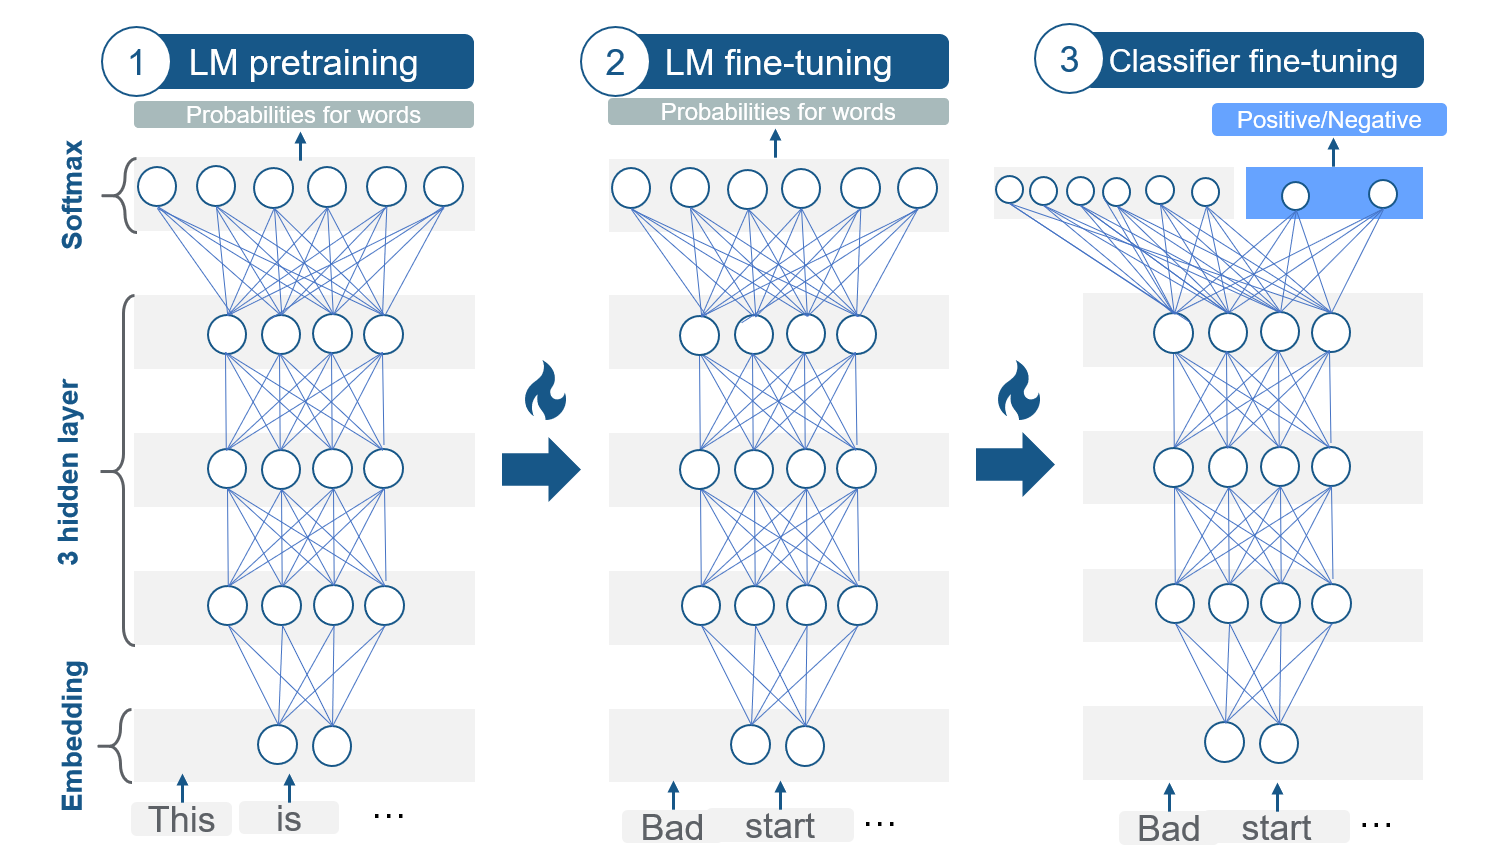
\includegraphics[width=0.9\textwidth]{ulmfit_process.png}
    \captionof{figure}{Quy trình 3 bước của ULMFiT: Pre-training trên dữ liệu chung, Fine-tuning LM trên dữ liệu miền đích, và Fine-tuning bộ phân loại cho tác vụ cuối cùng.}
    \label{fig:ulmfit_process}
\end{center}

\subsubsection{Các kỹ thuật Tinh chỉnh then chốt}
Sự thành công của ULMFiT không chỉ đến từ quy trình 3 bước mà còn từ 3 kỹ thuật tinh chỉnh thông minh được áp dụng trong bước cuối cùng.

\paragraph{1. Tinh chỉnh phân biệt (Discriminative Fine-tuning)}
Các tầng khác nhau của một mạng nơ-ron sâu nắm bắt các loại thông tin khác nhau: tầng đầu tiên học các đặc trưng rất chung chung, trong khi các tầng sau học các đặc trưng ngày càng cụ thể và phức tạp. Do đó, việc tinh chỉnh tất cả các tầng với cùng một tốc độ học (learning rate) là không hợp lý. ULMFiT đề xuất sử dụng các tốc độ học khác nhau cho mỗi tầng.

Giả sử mô hình có $L$ tầng, ta chọn một tốc độ học cơ sở $\eta_L$ cho tầng cuối cùng. Tốc độ học cho các tầng thấp hơn sẽ được tính bằng cách chia cho một hằng số (ví dụ: 2.6).
\[
\eta_{l-1} = \eta_l / \delta, \quad \text{với } \delta \text{ là một hằng số, ví dụ } 2.6.
\]
Khi cập nhật trọng số $\theta = \{\theta_1, \dots, \theta_L\}$, mỗi tầng sẽ được cập nhật như sau:
\begin{equation}
    \theta_l \leftarrow \theta_l - \eta_l \cdot \nabla_{\theta_l} J(\theta)
    \label{eq:discriminative_finetuning}
\end{equation}
Kỹ thuật này cho phép các tầng trên học hỏi nhanh chóng để thích nghi với tác vụ mới, trong khi các tầng dưới chỉ thay đổi một cách cẩn trọng để không làm mất đi kiến thức ngôn ngữ tổng quát đã học.

\paragraph{2. Tốc độ học Tam giác Lệch (Slanted Triangular Learning Rates - STLR)}
Thay vì giữ một tốc độ học không đổi hoặc giảm dần theo một hàm mũ đơn giản, ULMFiT sử dụng một lịch trình tốc độ học (learning rate schedule) đặc biệt. Trong một epoch, tốc độ học sẽ \textbf{tăng tuyến tính} trong một khoảng ngắn lúc đầu (warm-up), sau đó \textbf{giảm tuyến tính} trong phần còn lại của quá trình huấn luyện.

Công thức của STLR tại bước huấn luyện $t$ được định nghĩa như sau:
\begin{equation}
\eta_t = \eta_{\max} \times
\begin{cases}
    \frac{t}{t_{\text{cut}}} & \text{nếu } t < t_{\text{cut}} \\
    1 - \frac{t - t_{\text{cut}}}{T - t_{\text{cut}}} & \text{nếu } t \ge t_{\text{cut}}
\end{cases}
\label{eq:stlr}
\end{equation}
trong đó:
\begin{itemize}
    \item $T$ là tổng số bước huấn luyện trong một epoch.
    \item $t_{\text{cut}}$ là bước mà tại đó tốc độ học chuyển từ tăng sang giảm (thường là 10\% của $T$).
    \item $\eta_{\max}$ là tốc độ học tối đa, được chọn cho tầng cuối cùng. Các tầng khác sẽ có $\eta_{\max}$ riêng theo quy tắc của Tinh chỉnh phân biệt.
\end{itemize}
Chiến lược này giúp mô hình nhanh chóng hội tụ đến một vùng tham số tốt (giai đoạn tăng) rồi sau đó từ từ tinh chỉnh để tìm điểm tối ưu cục bộ tốt hơn (giai đoạn giảm).

\paragraph{3. Mở băng Dần dần (Gradual Unfreezing)}
Để tránh "sự quên lãng thảm khốc", việc tinh chỉnh toàn bộ mô hình ngay từ đầu trên một tập dữ liệu nhỏ có thể phá hỏng các trọng số đã được huấn luyện cẩn thận. ULMFiT đề xuất một phương pháp an toàn hơn, theo từng giai đoạn:

\begin{enumerate}
    \item \textbf{Giai đoạn 1:} Đóng băng (freeze) tất cả các tầng đã được huấn luyện trước ($l=1, \dots, L-1$), chỉ huấn luyện các tầng của đầu phân loại mới được thêm vào (tầng $L$) trong một epoch.
    \item \textbf{Giai đoạn 2:} Mở băng (unfreeze) tầng trên cùng của mô hình gốc (tầng $L-1$) và huấn luyện nó cùng với tầng $L$ trong một epoch nữa.
    \item \textbf{Giai đoạn 3 và tiếp theo:} Tiếp tục quá trình này, tuần tự mở băng từng tầng một từ trên xuống dưới ($L-2, L-3, \dots, 1$) và huấn luyện cho đến khi toàn bộ mô hình được tinh chỉnh.
\end{enumerate}
Phương pháp này giống như việc từ từ "rã đông" kiến thức, giúp mô hình thích nghi một cách nhẹ nhàng và hiệu quả, đặc biệt khi dữ liệu tác vụ có hạn.

\begin{tcolorbox}[
    title=Công thức thành công của ULMFiT,
    colback=green!5!white, colframe=green!50!black, fonttitle=\bfseries
]
ULMFiT không chỉ là một mô hình, mà là một công thức thực tiễn cho học chuyển giao trong NLP:
\begin{itemize}
    \item \textbf{Kiến trúc nền tảng:} AWD-LSTM (một biến thể LSTM hiệu quả và được điều chuẩn tốt).
    \item \textbf{Quy trình 3 bước:} Pre-train (chung) $\rightarrow$ Fine-tune LM (miền đích) $\rightarrow$ Fine-tune Classifier (tác vụ).
    \item \textbf{Bí quyết tinh chỉnh:} Kết hợp \textbf{Discriminative Fine-tuning}, \textbf{Slanted Triangular Learning Rates}, và \textbf{Gradual Unfreezing}.
\end{itemize}
\end{tcolorbox}

\subsubsection{Di sản và Hạn chế}
ULMFiT là một cột mốc quan trọng, nó đã "dân chủ hóa" việc áp dụng học chuyển giao trong NLP, cho thấy rằng không cần đến tài nguyên tính toán khổng lồ vẫn có thể đạt được hiệu suất cao. Nó đã đặt nền móng và tư duy cho các phương pháp sau này như BERT và các mô hình dựa trên Transformer, vốn cũng tuân theo quy trình "huấn luyện trước - tinh chỉnh" nhưng với kiến trúc mạnh mẽ hơn.

Tuy nhiên, hạn chế chính của ULMFiT nằm ở kiến trúc LSTM tuần tự, vốn không thể song song hóa hiệu quả và gặp khó khăn trong việc nắm bắt các phụ thuộc tầm xa so với kiến trúc Self-Attention của Transformer.


% % !TEX root = ../main.tex
% File: chapters_part1/chap3_7.tex
% Nội dung cho Phần 3.7: Các Kiến trúc Nơ-ron Khác

\section{Các Kiến trúc Nơ-ron Khác}
\label{sec:other_nn_architectures}

Bên cạnh RNN, CNN và các kiến trúc chính khác, trong NLP còn tồn tại nhiều hướng tiếp cận nơ-ron đặc thù cho các dạng bài toán riêng. Phần này sẽ trình bày hai kiến trúc tiêu biểu: \textbf{Mạng Siamese} cho việc học sự tương đồng, và \textbf{Mạng Nơ-ron Đồ thị (GNNs)} cho việc xử lý dữ liệu có cấu trúc đồ thị.

\subsection{Mạng Siamese (Siamese Networks) cho việc học sự tương đồng}
\label{ssec:siamese_networks}

Các kiến trúc chúng ta đã học như RNN hay CNN thường được huấn luyện cho các tác vụ phân loại (classification) hoặc gán nhãn (labeling). Tuy nhiên, có một lớp bài toán rất quan trọng trong NLP mà các kiến trúc này không trực tiếp giải quyết được: \textbf{đo lường sự tương đồng ngữ nghĩa (semantic similarity)} giữa hai câu. Ví dụ:
\begin{itemize}
    \item \textbf{Phát hiện câu hỏi trùng lặp (Duplicate Question Detection):} Trên các diễn đàn như Quora hay Stack Overflow, việc xác định xem một câu hỏi mới có trùng lặp về mặt ý nghĩa với một câu hỏi đã có hay không là rất quan trọng.
    \item \textbf{Tìm kiếm ngữ nghĩa (Semantic Search):} Tìm các tài liệu có ý nghĩa liên quan nhất đến một câu truy vấn, thay vì chỉ khớp từ khóa.
    \item \textbf{Đánh giá câu trả lời của sinh viên (Automatic Short Answer Grading):} So sánh câu trả lời của sinh viên với câu trả lời mẫu để chấm điểm.
\end{itemize}

Để giải quyết các bài toán này, chúng ta cần một mô hình có khả năng nhận vào hai câu và xuất ra một điểm số thể hiện mức độ tương đồng của chúng. Mạng Siamese \cite{mueller2016siamese} là một kiến trúc thanh lịch và mạnh mẽ được thiết kế cho chính mục đích này.

\subsubsection{Tư duy cốt lõi: Học một không gian biểu diễn tốt}
\label{ssec:siamese_intuition}

Thay vì cố gắng học một hàm phân loại trực tiếp trên cặp câu, ý tưởng cốt lõi của Mạng Siamese là \textbf{học một hàm nhúng (embedding function) có khả năng ánh xạ các câu vào một không gian vector (embedding space) sao cho trong không gian đó, khoảng cách giữa các câu có thể phản ánh sự tương đồng về mặt ngữ nghĩa của chúng}.

Nói một cách cụ thể hơn, Mạng Siamese học cách để:
\begin{itemize}
    \item Các cặp câu \textbf{tương tự} (similar pairs) được kéo lại \textbf{gần nhau} trong không gian embedding.
    \item Các cặp câu \textbf{không tương tự} (dissimilar pairs) bị đẩy ra \textbf{xa nhau} trong không gian embedding.
\end{itemize}

Sau khi đã học được không gian embedding tốt này, việc đo độ tương đồng giữa hai câu mới chỉ đơn giản là ánh xạ chúng vào không gian này và tính khoảng cách Euclide hoặc độ tương đồng cosine giữa hai vector kết quả.

\subsubsection{Kiến trúc Mạng Siamese}
\label{ssec:siamese_architecture}

Cái tên "Siamese" (cặp song sinh dính liền) mô tả rất chính xác kiến trúc của nó. Mạng Siamese bao gồm hai "nhánh" (towers) mạng nơ-ron giống hệt nhau, xử lý hai đầu vào một cách song song.

\paragraph{Hai nhánh, một bộ não}
\begin{itemize}
    \item Mạng bao gồm hai bộ mã hóa (encoder) có \textbf{kiến trúc y hệt nhau}.
    \item Quan trọng nhất, hai bộ mã hóa này \textbf{chia sẻ cùng một bộ trọng số (share weights)}. Điều này có nghĩa là chúng ta chỉ có một "bộ não" duy nhất, được áp dụng cho cả hai câu đầu vào.
    \item Việc chia sẻ trọng số đảm bảo rằng hai câu giống hệt nhau sẽ luôn được ánh xạ tới cùng một điểm trong không gian embedding. Nó cũng làm cho mô hình hiệu quả hơn nhiều về mặt tham số.
    \item Bộ mã hóa này có thể là bất kỳ kiến trúc nào có khả năng biến một chuỗi thành một vector, ví dụ như một mạng LSTM, GRU, hoặc CNN đã được học ở các phần trước.
\end{itemize}

\begin{center}
    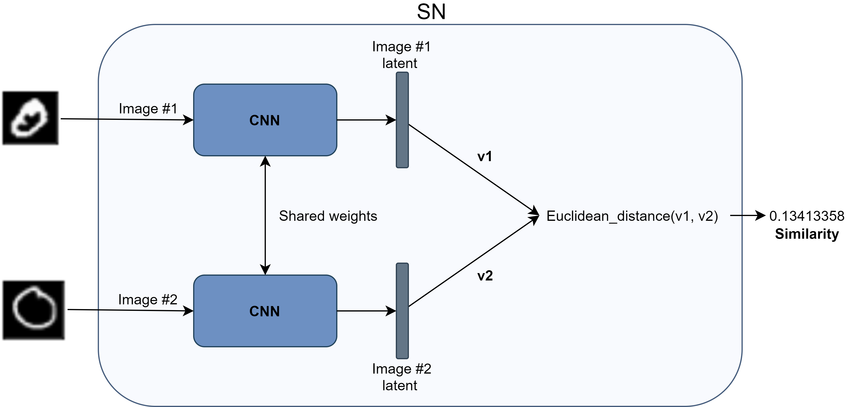
\includegraphics[width=0.7\textwidth]{siamese_network_architecture.png}
    \captionof{figure}{Kiến trúc của Mạng Siamese. Hai mạng con (thường là LSTM hoặc CNN) có cùng kiến trúc và chia sẻ trọng số. Chúng xử lý hai câu đầu vào để tạo ra hai vector embedding. Hàm mất mát sau đó được tính toán dựa trên khoảng cách giữa hai vector này.}
    \label{fig:siamese_network_architecture}
\end{center}

\subsubsection{Hàm Mất mát Tương phản (Contrastive Loss)}
\label{ssec:contrastive_loss}
Kiến trúc chỉ là một nửa câu chuyện. Phép màu thực sự của Mạng Siamese nằm ở hàm mất mát đặc biệt được sử dụng để huấn luyện nó: \textbf{Hàm Mất mát Tương phản (Contrastive Loss) \cite{hadsell2006dimensionality}}.

Hàm mất mát này được thiết kế để thực hiện chính xác mục tiêu mà chúng ta đã đề ra: kéo các cặp tương tự lại gần và đẩy các cặp không tương tự ra xa.

\paragraph{Đầu vào huấn luyện}
Để huấn luyện với Contrastive Loss, chúng ta cần một bộ dữ liệu bao gồm các bộ ba: (\texttt{câu\_A}, \texttt{câu\_B}, nhãn).
\begin{itemize}
    \item \textbf{Nhãn $Y=1$ (Cặp Tương tự):} \texttt{câu\_A} và \texttt{câu\_B} có cùng ý nghĩa.
    \item \textbf{Nhãn $Y=0$ (Cặp Không Tương tự):} \texttt{câu\_A} và \texttt{câu\_B} có ý nghĩa khác nhau.
\end{itemize}


\paragraph{Công thức}
Cho một cặp đầu vào, Mạng Siamese tạo ra một cặp vector embedding $(v_A, v_B)$. Chúng ta định nghĩa $D_W$ là khoảng cách Euclide giữa chúng: $D_W = ||v_A - v_B||_2$.

Hàm mất mát tương phản được định nghĩa như sau:
\begin{equation}
    \text{Loss}(W, (Y, v_A, v_B)) = Y \cdot \frac{1}{2} D_W^2 + (1-Y) \cdot \frac{1}{2} \max(0, m - D_W)^2
    \label{eq:contrastive_loss}
\end{equation}
Trong đó $m$ là một siêu tham số gọi là \textbf{lề (margin)}.

\paragraph{Phân tích hàm mất mát}
Hãy xem hàm mất mát này hoạt động như thế nào trong hai trường hợp:
\begin{enumerate}
    \item \textbf{Khi cặp câu là Tương tự ($Y=1$):}
        \begin{itemize}
            \item Phần thứ hai của công thức bị triệt tiêu (vì $1-Y=0$).
            \item Hàm mất mát trở thành: $\text{Loss} = \frac{1}{2} D_W^2$.
            \item Để tối thiểu hóa loss, mô hình phải làm cho khoảng cách $D_W$ càng gần 0 càng tốt. Điều này \textbf{kéo hai vector lại gần nhau}.
        \end{itemize}
    \item \textbf{Khi cặp câu là Không Tương tự ($Y=0$):}
        \begin{itemize}
            \item Phần đầu của công thức bị triệt tiêu (vì $Y=0$).
            \item Hàm mất mát trở thành: $\text{Loss} = \frac{1}{2} \max(0, m - D_W)^2$.
            \item Để tối thiểu hóa loss, mô hình phải làm cho $m - D_W$ nhỏ hơn hoặc bằng 0, tức là $D_W \geq m$.
            \item Điều này \textbf{đẩy hai vector ra xa nhau} cho đến khi khoảng cách giữa chúng ít nhất là bằng lề $m$. Nếu chúng đã đủ xa ($D_W > m$), loss sẽ bằng 0 và mô hình không cần phải làm gì thêm.
        \end{itemize}
\end{enumerate}
Lề $m$ đóng vai trò như một "vùng an toàn", nó yêu cầu các cặp không tương tự phải cách nhau một khoảng tối thiểu, tạo ra sự phân tách rõ ràng trong không gian embedding.

\subsubsection{Triplet Loss: Một sự thay thế nâng cao}
\label{ssec:triplet_loss}

Một hàm mất mát phổ biến khác, có liên quan chặt chẽ, là \textbf{Triplet Loss \cite{schroff2015facenet}}. Thay vì huấn luyện trên các cặp, Triplet Loss huấn luyện trên các bộ ba (triplets) gồm:
\begin{itemize}
    \item \textbf{Anchor (A):} Một câu neo.
    \item \textbf{Positive (P):} Một câu tương tự với Anchor.
    \item \textbf{Negative (N):} Một câu không tương tự với Anchor.
\end{itemize}

Mục tiêu của Triplet Loss là làm cho khoảng cách từ Anchor đến Positive nhỏ hơn khoảng cách từ Anchor đến Negative, cộng với một lề $m$.
$$ d(A, P) + m < d(A, N) $$
Hàm mất mát được định nghĩa là:
\begin{equation}
    \text{Loss} = \max(0, d(A, P) - d(A, N) + m)
    \label{eq:triplet_loss}
\end{equation}
Triplet Loss thường được coi là mạnh mẽ hơn vì nó trực tiếp tối ưu hóa thứ hạng tương đối giữa các câu, thay vì chỉ xem xét các cặp một cách riêng lẻ. Tuy nhiên, việc tạo ra các bộ ba huấn luyện hiệu quả (hard triplets) là một thách thức kỹ thuật.

\subsubsection{Tổng kết}
Mạng Siamese và các hàm mất mát đi kèm (Contrastive/Triplet Loss) là một bộ công cụ cực kỳ mạnh mẽ cho các bài toán so sánh. Chúng không chỉ giới hạn trong NLP mà còn được áp dụng rộng rãi trong xử lý ảnh để nhận dạng khuôn mặt (face verification) hay tìm kiếm ảnh tương tự.

Thay vì học cách phân loại, Mạng Siamese học cách \textbf{biểu diễn}, tạo ra các embedding chất lượng cao, có thể tái sử dụng cho nhiều tác vụ hạ nguồn liên quan đến đo lường sự tương đồng.

\subsection{Mạng Nơ-ron Đồ thị (Graph Neural Networks - GNNs) trong NLP}
\label{ssec:gnn_for_nlp}

Trong suốt chương này, chúng ta đã xem xét các kiến trúc được thiết kế để xử lý dữ liệu dạng \textbf{chuỗi (sequences)} như RNN và các kiến trúc trích xuất đặc trưng cục bộ như CNN. Tuy nhiên, một sự thật quan trọng là: \textbf{ngôn ngữ không phải lúc nào cũng là một chuỗi tuyến tính}. Rất nhiều thông tin quý giá trong ngôn ngữ và thế giới mà nó mô tả lại có cấu trúc của một \textbf{đồ thị (graph)}.

Ví dụ:
\begin{itemize}
    \item Cấu trúc cú pháp của một câu (như Cú pháp Phụ thuộc đã học ở Chương 1) là một đồ thị.
    \item Một cơ sở tri thức (Knowledge Base) về các thực thể và mối quan hệ của chúng là một đồ thị.
    \item Một mạng xã hội, với người dùng và mối quan hệ bạn bè, là một đồ thị.
    \item Một cuộc hội thoại nhiều bên, với các lượt lời và quan hệ trả lời, là một đồ thị.
\end{itemize}

Các kiến trúc truyền thống như RNN và CNN gặp khó khăn trong việc mô hình hóa các mối quan hệ phức tạp, không tuần tự này. Mạng Nơ-ron Đồ thị (GNNs) \cite{scarselli2009graph, kipf2016semi} ra đời như một giải pháp tổng quát và mạnh mẽ để học trực tiếp trên dữ liệu có cấu trúc đồ thị.

\subsubsection{Nguyên lý Cốt lõi của GNN: Lan truyền Thông điệp (Message Passing)}
\label{ssec:gnn_message_passing}

Để hiểu GNN, trước hết ta cần hiểu cách nó "suy nghĩ" về một đồ thị. Một đồ thị bao gồm các \textbf{nút (nodes)} và các \textbf{cạnh (edges)} nối giữa chúng. Trong GNN, mỗi nút có một vector đặc trưng (node feature vector) riêng. Mục tiêu của GNN là học một hàm để tính toán một \textbf{vector biểu diễn (node representation/embedding)} cho mỗi nút, sao cho vector này không chỉ chứa thông tin của chính nút đó mà còn tóm tắt được thông tin từ \textbf{cấu trúc lân cận} của nó.

GNN thực hiện điều này thông qua một quy trình lặp đi lặp lại gọi là \textbf{Lan truyền Thông điệp (Message Passing)} hoặc \textbf{Tổng hợp Lân cận (Neighborhood Aggregation)}.

\begin{tcolorbox}[
    title=Trực giác về Lan truyền Thông điệp,
    colback=green!5!white, colframe=green!60!black, fonttitle=\bfseries
]
Hãy tưởng tượng mỗi nút trong đồ thị là một người. Tại mỗi vòng, mỗi người sẽ làm hai việc:
\begin{enumerate}
    \item \textbf{Gửi thư:} Gửi một bản sao "trạng thái" hiện tại của mình cho tất cả những người hàng xóm.
    \item \textbf{Cập nhật bản thân:} Nhận tất cả "thư" từ hàng xóm, tổng hợp chúng lại thành một thông điệp duy nhất, và sau đó kết hợp thông điệp này với trạng thái cũ của mình để tạo ra một trạng thái mới, thông thái hơn.
\end{enumerate}
Khi quá trình này lặp lại nhiều lần, thông tin từ những nút ở xa sẽ dần dần lan truyền khắp đồ thị. Một nút sau $k$ vòng lặp sẽ có một vector biểu diễn chứa thông tin từ tất cả các nút cách nó $k$ bước chân.
\end{tcolorbox}

Về mặt kỹ thuật, một lớp GNN thực hiện 3 bước:
\begin{enumerate}
    \item \textbf{Thu thập (Gather):} Với mỗi nút, thu thập vector đặc trưng từ tất cả các nút hàng xóm trực tiếp của nó.
    \item \textbf{Tổng hợp (Aggregate):} Áp dụng một hàm tổng hợp (ví dụ: `SUM`, `MEAN`, `MAX`) lên các vector đã thu thập để tạo ra một "thông điệp" lân cận duy nhất. Hàm này phải không nhạy cảm với thứ tự của các hàng xóm.
    \item \textbf{Cập nhật (Update):} Kết hợp thông điệp lân cận với vector đặc trưng hiện tại của nút (thường thông qua một mạng nơ-ron nhỏ) để tạo ra vector đặc trưng mới cho nút đó ở lớp tiếp theo.
\end{enumerate}

\begin{center}
    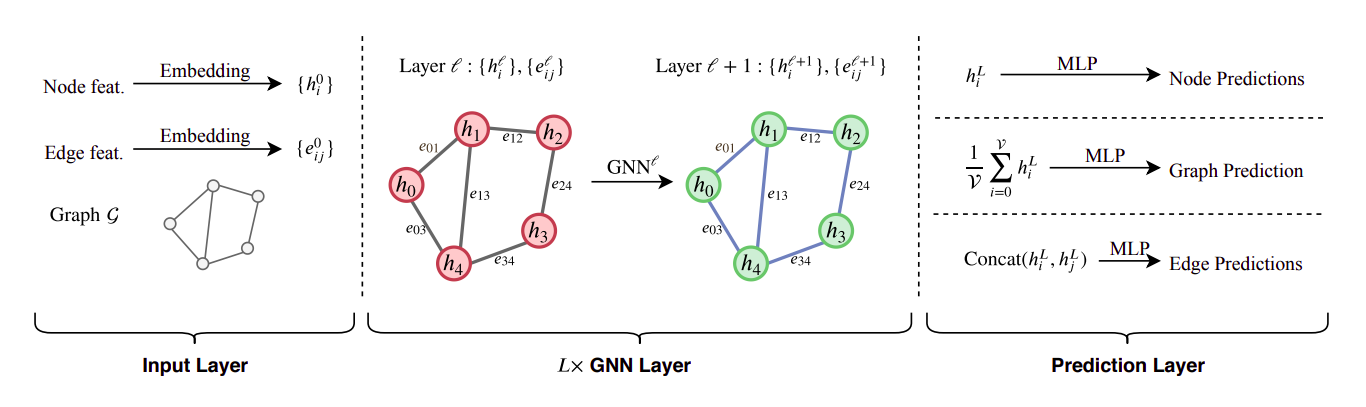
\includegraphics[width=1.0\textwidth]{gnn_message_passing.png}
    \captionof{figure}{Quy trình Lan truyền Thông điệp trong một lớp GNN. Nút A cập nhật trạng thái của nó bằng cách tổng hợp thông tin từ các hàng xóm B, C, D.}
    \label{fig:gnn_message_passing}
\end{center}

Bằng cách xếp chồng nhiều lớp GNN, một nút có thể tích hợp thông tin từ các hàng xóm ngày càng xa, cho phép mô hình có được "cái nhìn toàn cảnh" về vị trí và vai trò của mỗi nút trong toàn bộ đồ thị.

\subsubsection{Huấn luyện GNN}
Quá trình huấn luyện một GNN phụ thuộc vào tác vụ cụ thể ở cấp độ đồ thị, nút, hoặc cạnh.
\begin{itemize}
    \item \textbf{Tạo biểu diễn nút:} Sau $k$ lớp Message Passing, mỗi nút sẽ có một vector biểu diễn cuối cùng $h_v^{(k)}$ chứa thông tin từ lân cận $k$-bước của nó.
    \item \textbf{Hàm Mất mát:} Vector biểu diễn này sau đó được đưa vào một lớp đầu ra (ví dụ, một lớp FNN) để thực hiện dự đoán.
        \begin{itemize}
            \item \textbf{Phân loại Nút:} Lỗi (ví dụ, Cross-Entropy) được tính toán cho từng nút và lan truyền ngược qua các lớp GNN để cập nhật các trọng số của hàm tổng hợp (Aggregate) và cập nhật (Update).
            \item \textbf{Phân loại Đồ thị:} Các biểu diễn của tất cả các nút trong đồ thị được tổng hợp lại (ví dụ, qua pooling) thành một vector biểu diễn đồ thị duy nhất trước khi đưa vào lớp phân loại.
        \end{itemize}
\end{itemize}
Tương tự như các mạng khác, toàn bộ quá trình được tối ưu hóa end-to-end thông qua backpropagation.

\subsubsection{Các Ứng dụng then chốt của GNN trong NLP}
\label{ssec:gnn_applications}

Với khả năng học trên cấu trúc, GNN mở ra nhiều hướng ứng dụng mạnh mẽ trong NLP.

\paragraph{Làm việc với Đồ thị Tri thức và Mạng xã hội}
Đây là ứng dụng tự nhiên nhất của GNN. Trong một \textbf{Đồ thị Tri thức (Knowledge Graph - KG)}, các nút là các thực thể (ví dụ: `Hà Nội`, `Việt Nam`) và các cạnh có nhãn là các mối quan hệ (ví dụ: `isCapitalOf`).
GNN được sử dụng để giải quyết hai bài toán chính:
\begin{itemize}
    \item \textbf{Phân loại Nút (Node Classification):} Dự đoán một thuộc tính còn thiếu của một thực thể. Ví dụ, dự đoán thể loại của một bộ phim dựa trên các diễn viên và đạo diễn (các nút lân cận) của nó.
    \item \textbf{Dự đoán Liên kết (Link Prediction):} Đây là bài toán \textbf{trích xuất quan hệ và suy luận logic}. Mô hình dự đoán xem liệu một cạnh (mối quan hệ) có nên tồn tại giữa hai nút hay không. Ví dụ, nếu KG có các cạnh `(David Beckham, playsFor, Manchester United)` và `(Manchester United, locatedIn, England)`, GNN có thể học cách suy luận ra một liên kết tiềm năng `(David Beckham, hasNationality, English)`. Điều này cho phép tự động hoàn thiện và mở rộng các KG.
\end{itemize}

\paragraph{Phân tích Cú pháp dựa trên Đồ thị (Graph-based Parsing)}
Như đã đề cập, cây cú pháp phụ thuộc của một câu là một đồ thị. Chúng ta có thể áp dụng GNN trực tiếp lên cấu trúc này.
\begin{itemize}
    \item \textbf{Biểu diễn ngữ nghĩa dựa trên cấu trúc (Structure-aware Semantic Representation):} Thay vì chỉ dựa vào thứ tự tuần tự như LSTM, GNN cho phép một từ được biểu diễn bởi một vector tổng hợp thông tin từ các từ "quản lý" và "phụ thuộc" của nó. Ví dụ, vector của một động từ sẽ được "làm giàu" bởi thông tin từ chủ ngữ và tân ngữ của nó. Các biểu diễn này thường nắm bắt ngữ nghĩa chức năng tốt hơn.
    \item \textbf{Cải thiện các tác vụ hạ nguồn:} Các biểu diễn giàu cú pháp này sau đó có thể được sử dụng để cải thiện hiệu năng của các tác vụ như Trích xuất Quan hệ hay Phân tích Cảm xúc.
\end{itemize}

\paragraph{Mô hình hóa Hội thoại (Dialogue Modeling)}
Một cuộc hội thoại, đặc biệt là với nhiều người tham gia, không phải là một chuỗi tuyến tính.
\begin{itemize}
    \item \textbf{Xây dựng Đồ thị Hội thoại (Dialogue Graph):} Chúng ta có thể xây dựng một đồ thị trong đó các nút là các lượt lời (utterances), và các cạnh biểu diễn các mối quan hệ như "ai trả lời ai" hoặc "các lượt lời của cùng một người".
    \item \textbf{Ứng dụng GNN:} GNN có thể được chạy trên đồ thị này để học biểu diễn cho mỗi lượt lời, có tính đến toàn bộ lịch sử tương tác. Điều này rất hữu ích cho các tác vụ như tóm tắt hội thoại, theo dõi trạng thái hội thoại (dialogue state tracking), hoặc xác định cảm xúc trong các cuộc trò chuyện phức tạp.
\end{itemize}

\subsubsection{Các Kiến trúc Lai ghép: Kết hợp GNN và Transformer}
\label{ssec:gnn_transformer}

Sự ra đời của Transformer (sẽ học ở chương sau) đã thống trị NLP với khả năng nắm bắt phụ thuộc tầm xa trong chuỗi. Tuy nhiên, Transformer vốn không được thiết kế để xử lý thông tin cấu trúc tường minh. Điều này đã dẫn đến một hướng nghiên cứu sôi nổi: \textbf{kết hợp GNN và Transformer}.
\begin{itemize}
    \item \textbf{Ý tưởng:} Sử dụng Transformer để có được các biểu diễn từ ban đầu, giàu ngữ cảnh tuần tự. Sau đó, xây dựng một đồ thị (ví dụ: đồ thị cú pháp) lên trên các từ này và sử dụng GNN để "tinh chỉnh" (refine) các biểu diễn đó bằng cách cho chúng lan truyền thông tin qua cấu trúc đồ thị.
    \item \textbf{Kết quả:} Các mô hình lai ghép này thường cho kết quả tốt hơn trên các tác vụ đòi hỏi cả sự hiểu biết về cấu trúc và ngữ cảnh, ví dụ như các bài toán suy luận phức tạp.
\end{itemize}

\subsubsection{Thách thức và Hướng nghiên cứu Tương lai}
\label{ssec:gnn_challenges}
Mặc dù rất mạnh mẽ, GNN vẫn phải đối mặt với nhiều thách thức:
\begin{itemize}
    \item \textbf{Khả năng mở rộng (Scalability):} Áp dụng GNN trên các đồ thị web-scale với hàng tỷ nút và cạnh là một thách thức lớn về mặt tính toán và bộ nhớ.
    \item \textbf{Đồ thị Động (Dynamic Graphs):} Hầu hết các GNN giả định một cấu trúc đồ thị tĩnh. Việc xử lý các đồ thị thay đổi liên tục theo thời gian (như mạng xã hội) vẫn là một lĩnh vực nghiên cứu tích cực.
    \item \textbf{Làm mịn quá mức (Over-smoothing):} Khi xếp chồng quá nhiều lớp GNN, các biểu diễn của tất cả các nút có xu hướng hội tụ về cùng một giá trị, làm mất đi thông tin cục bộ. Đây là một vấn đề cố hữu của GNN.
    \item \textbf{Đồ thị nhiễu và không hoàn chỉnh:} Làm thế nào để mô hình hoạt động mạnh mẽ khi cấu trúc đồ thị đầu vào bị nhiễu hoặc thiếu các cạnh quan trọng?
\end{itemize}

Bất chấp những thách thức này, GNN đại diện cho một hướng đi quan trọng, giúp NLP vượt ra khỏi giới hạn của chuỗi tuần tự và tiến tới việc mô hình hóa các mối quan hệ phức tạp hơn, một bước gần hơn đến việc thực sự hiểu được ngôn ngữ.
% % !TEX root = ../main.tex
% File: chapters_part1/chap3_8.tex
% Nội dung cho Phần 3.8: Các Mô hình Sinh Tiền-Transformer

\section{Các Mô hình Sinh Tiền-Transformer (Pre-Transformer Generative Models)}
\label{sec:pre_transformer_generative}

Trước khi Transformer định hình lại toàn bộ lĩnh vực NLP, cộng đồng nghiên cứu đã dành nhiều nỗ lực để xây dựng các \textbf{mô hình sinh} (generative models) cho văn bản. Khác với các mô hình phân loại hay dịch máy vốn chỉ cần \textit{hiểu} hoặc \textit{chuyển đổi} ngôn ngữ, mô hình sinh có mục tiêu tham vọng hơn: \textbf{sáng tạo ngôn ngữ mới}, ví dụ như viết một đoạn hội thoại, một bài thơ, hay một câu nhận xét sản phẩm mà vẫn mạch lạc và hợp lý.

Trong giai đoạn 2015–2017, hai hướng tiếp cận chính cho bài toán sinh văn bản nổi bật: \textbf{Variational Autoencoders (VAEs)} và \textbf{Generative Adversarial Networks (GANs)}. Việc tìm hiểu chúng mang lại giá trị lịch sử và giúp ta thấy rõ những thách thức cố hữu trong việc sinh dữ liệu rời rạc như văn bản.

\subsection{Variational Autoencoder (VAE) cho Văn bản}
\label{ssec:vae_for_text}

\paragraph{Ý tưởng cốt lõi.}  
Khác với Autoencoder thường (đã trình bày ở Mục~\ref{ssec:autoencoders}), \textbf{VAE} (Kingma \& Welling, 2013) \cite{kingma2013auto} coi không gian ẩn là một \textit{phân phối xác suất}. Thay vì ánh xạ đầu vào $x$ thành một vector điểm $\mathbf{z}$, Encoder ánh xạ thành $q_\phi(z|x) \sim \mathcal{N}(\mu, \sigma^2)$, từ đó lấy mẫu $z$ và giải mã bằng Decoder.

\paragraph{Hàm mất mát ELBO.}  
Mục tiêu huấn luyện là cực đại hoá cận dưới hợp lý hóa bằng chứng:
\[
\mathcal{L}_{VAE}(x) = \mathbb{E}_{q_\phi(z|x)} \left[ \log p_\theta(x|z) \right] - KL\left(q_\phi(z|x)\;||\;p(z)\right)
\]
Trong đó $KL(\cdot||\cdot)$ đo khoảng cách giữa phân phối hậu nghiệm xấp xỉ và tiên nghiệm $p(z)$ (thường là Gaussian chuẩn).

\begin{tcolorbox}[title={Ưu điểm của VAE cho văn bản}, colback=purple!5!white, colframe=purple!75!black, fonttitle=\bfseries]
\begin{itemize}
    \item \textbf{Khả năng sinh}: lấy mẫu $z$ từ $\mathcal{N}(0,I)$ và giải mã ra văn bản mới.  
    \item \textbf{Nội suy không gian ẩn}: kết hợp hai vector $z_1, z_2$ để sinh ra văn bản trung gian.  
    \item \textbf{Ứng dụng}: sinh câu đa dạng (Bowman et al., 2016), style transfer.  
\end{itemize}
\end{tcolorbox}

\paragraph{Thách thức: Posterior Collapse.}  
Decoder mạnh (LSTM/GRU) dễ dàng \textbf{lờ $z$}, chỉ dự đoán từ tiếp theo dựa vào lịch sử ⇒ khiến không gian ẩn mất ý nghĩa. Đây là một vấn đề được chỉ ra trong các công trình đầu tiên áp dụng VAE cho văn bản \cite{bowman2015generating}.

\textbf{Giải pháp:}
\begin{itemize}
    \item KL-annealing (tăng dần trọng số KL).  
    \item Free-bits (ép mỗi chiều KL có đóng góp tối thiểu).  
    \item $\beta$-VAE (điều chỉnh trade-off giữa likelihood và KL).  
\end{itemize}

\subsection{Generative Adversarial Networks (GANs) cho Văn bản}
\label{ssec:gan_for_text}

\paragraph{Ý tưởng cơ bản.}  
GAN (Goodfellow et al., 2014) \cite{goodfellow2014generative} là một trò chơi đối kháng:
\begin{itemize}
    \item \textbf{Generator $G$}: sinh văn bản giả từ vector nhiễu $z$.  
    \item \textbf{Discriminator $D$}: phân biệt văn bản thật từ dữ liệu và văn bản giả từ $G$.  
\end{itemize}

\paragraph{Vấn đề rời rạc.}  
Khác ảnh (dữ liệu liên tục), văn bản là \textbf{chuỗi rời rạc}. Việc chọn từ (qua \texttt{argmax}) không khả vi, gradient từ $D$ không truyền ngược về $G$.  

\textbf{Các hướng giải quyết:}
\begin{itemize}
    \item \textbf{Học tăng cường}:  
        - SeqGAN (2017): dùng policy gradient.  
        - MaliGAN (2017): cải thiện reward shaping.  
        - LeakGAN (2018): cho $D$ “rò rỉ” trạng thái cho $G$.  
    \item \textbf{Xấp xỉ liên tục}:  
        - Gumbel-Softmax để làm trơn \texttt{argmax}.  
        - RelGAN (2019): training ổn định hơn.  
\end{itemize}

\paragraph{Hạn chế thực tiễn.}  
GAN cho văn bản huấn luyện khó và thiếu ổn định, nên chỉ dừng lại ở mức nghiên cứu, chưa có ứng dụng rộng như GAN trong ảnh.

\subsection{So sánh VAE và GAN trong Sinh Văn bản}
\label{ssec:vae_gan_compare}

\begin{table}[H]
\centering
\begin{tabular}{|p{3cm}|p{5cm}|p{5cm}|}
\hline
\textbf{Tiêu chí} & \textbf{VAE} & \textbf{GAN} \\ \hline
Nguyên lý & Xác suất, tối ưu ELBO (likelihood-based) & Đối kháng, min-max game \\ \hline
Đầu ra & Đa dạng, có thể nội suy latent & Có thể sắc nét, nhưng không ổn định \\ \hline
Thách thức & Posterior collapse & Không khả vi, gradient vanishing \\ \hline
Ứng dụng chính & Sinh câu, style transfer & Chủ yếu học thuật, ít thực tiễn \\ \hline
\end{tabular}
\caption{So sánh VAE và GAN trong sinh văn bản trước Transformer.}
\label{tab:vae_gan_compare}
\end{table}

\subsection{Chuyển tiếp sang Kỷ nguyên Transformer}
\label{ssec:transition_to_transformer}

VAE và GAN đặt nền móng cho ý tưởng sinh văn bản, nhưng gặp giới hạn về độ ổn định và khả năng mở rộng. Sự ra đời của \textbf{Transformer} (Vaswani et al., 2017) đã thay đổi toàn bộ cục diện:
\begin{itemize}
    \item Self-attention mô hình hóa phụ thuộc dài tốt hơn RNN.  
    \item Huấn luyện likelihood trực tiếp (mô hình ngôn ngữ) ổn định hơn GAN.  
    \item Kiến trúc dễ mở rộng quy mô lớn, tạo tiền đề cho GPT và các LLM sau này.  
\end{itemize}

Do đó, các mô hình sinh tiền-Transformer (VAE, GAN) nên được coi là \textbf{bước đệm lịch sử}, giúp rút ra nhiều bài học quan trọng trước khi cộng đồng chuyển sang các mô hình ngôn ngữ sinh hiện đại dựa trên Transformer.

\bigskip
\hrule
\bigskip

\begin{center}
    \textbf{\Large KẾT THÚC CHƯƠNG 3}
\end{center}

\textit{Trong chương này, chúng ta đã khám phá một "vườn thú" các kiến trúc mạng nơ-ron đã định hình nên kỷ nguyên học sâu của NLP. Từ khả năng ghi nhớ của RNN/LSTM, đến sức mạnh trích xuất đặc trưng của CNN, và khả năng học trên các cấu trúc phức tạp của GNN. Quan trọng nhất, chúng ta đã chứng kiến sự ra đời của cơ chế Chú ý (Attention) trong mô hình Seq2Seq. Cơ chế Chú ý, ban đầu chỉ là một thành phần bổ trợ, đã tỏ ra mạnh mẽ đến mức nó đặt ra một câu hỏi mang tính cách mạng: Liệu chúng ta có thể xây dựng một kiến trúc hoàn toàn từ bỏ các vòng lặp hồi tiếp và chỉ dựa vào sự chú ý không? Câu trả lời cho câu hỏi này sẽ mở ra chương tiếp theo và cũng là kỷ nguyên hiện đại của NLP: Kỷ nguyên Transformer.}

% \chapter{CÁC KIẾN TRÚC MẠNG NƠ-RON KINH ĐIỂN}
\label{chap:deep_learning_architectures}

Chào mừng bạn đến với kỷ nguyên học sâu của NLP. Trong chương 2, chúng ta đã thấy các mô hình thống kê như N-gram có thể nắm bắt các phụ thuộc cục bộ, nhưng lại bất lực trước các mối quan hệ tầm xa. Cuộc cách mạng word embedding đã cho chúng ta các vector từ mang đầy ngữ nghĩa, nhưng làm thế nào để kết hợp chúng lại nhằm hiểu được ý nghĩa của cả một câu hay một đoạn văn?

Chương này sẽ giới thiệu các kiến trúc mạng nơ-ron nền tảng được thiết kế đặc biệt để xử lý dữ liệu dạng chuỗi như ngôn ngữ tự nhiên. Những kiến trúc này không chỉ đơn thuần "nhìn" vào các từ một cách riêng lẻ, mà còn có khả năng "ghi nhớ" và "lý luận" dựa trên thông tin đã xử lý trước đó, cho phép chúng nắm bắt được ngữ cảnh và các phụ thuộc phức tạp trong câu.
% % !TEX root = ../main.tex
% File: chapters_part1/chap4_1.tex
% Nội dung cho Chương 4, Phần 1

\section{Kiến trúc Transformer Gốc ("Attention Is All You Need")}
\label{sec:vanilla_transformer}

Để hiểu được sức mạnh của Transformer, chúng ta cần mổ xẻ từng khối xây dựng nên nó, bắt đầu từ ý tưởng cốt lõi nhất: Self-Attention.

\subsection{Chi tiết cơ chế Self-Attention: Scaled Dot-Product và Multi-Head Attention}
\label{ssec:self_attention}

Cơ chế chú ý mà chúng ta đã học trong mô hình Seq2Seq (ở mục \ref{sec:seq2seq_attention}) là \textit{cross-attention}, nơi Decoder "chú ý" đến Encoder. \textbf{Self-Attention (Tự chú ý)} là một biến thể đặc biệt, nơi một chuỗi "chú ý" đến chính nó.

\paragraph{Tư duy cốt lõi}
Self-Attention cho phép mỗi từ trong một câu có thể "nhìn" vào tất cả các từ khác trong cùng một câu để tính toán ra một biểu diễn mới cho chính nó. Biểu diễn mới này không chỉ chứa thông tin của bản thân từ đó, mà còn được "làm giàu" bởi ngữ cảnh từ các từ liên quan nhất.

Ví dụ, trong câu "Con mèo không muốn băng qua đường vì nó quá mệt", khi xử lý từ "nó", Self-Attention sẽ giúp mô hình xác định rằng "nó" có liên quan mật thiết đến "mèo" chứ không phải "đường", và tạo ra một biểu diễn cho "nó" mang nhiều thông tin của "mèo".

\subsubsection{Scaled Dot-Product Attention}
Đây là khối xây dựng cơ bản của Self-Attention trong Transformer. Nó hoạt động dựa trên ba khái niệm được lấy cảm hứng từ các hệ thống tìm kiếm thông tin: \textbf{Query, Key, và Value}.

\begin{tcolorbox}[
    title={Trực giác về Query, Key, Value},
    colback=yellow!10!white, colframe=yellow!50!black, fonttitle=\bfseries
]
Hãy tưởng tượng bạn đang tìm kiếm video trên YouTube.
\begin{itemize}
    \item \textbf{Query (Truy vấn):} Là cụm từ bạn gõ vào thanh tìm kiếm (ví dụ: "công thức nấu phở"). Nó đại diện cho \textit{thông tin bạn đang cần}.
    \item \textbf{Key (Khóa):} Mỗi video trên YouTube có một bộ các từ khóa (tiêu đề, mô tả) để mô tả nội dung của nó. Nó đại diện cho \textit{thông tin mà một đối tượng có thể cung cấp}.
    \item \textbf{Value (Giá trị):} Chính là nội dung của video. Nó đại diện cho \textit{thông tin thực sự sẽ được lấy ra}.
\end{itemize}
Cơ chế hoạt động là: bạn lấy \textbf{Query} của mình, so sánh nó với \textbf{Key} của tất cả các video để tìm ra các video liên quan nhất (tính điểm tương đồng). Sau đó, bạn lấy một "tổng có trọng số" của các \textbf{Value} (nội dung video), trong đó các video liên quan hơn sẽ có trọng số cao hơn.
\end{tcolorbox}

\begin{tcolorbox}[
    title={Tại sao lại cần đến ba vai trò Q, K, V?},
    colback=green!5!white, colframe=green!50!black, fonttitle=\bfseries
]
Một câu hỏi tự nhiên là: Tại sao mỗi từ đầu vào $x_i$ lại cần được chiếu thành ba vector $q_i, k_i, v_i$ riêng biệt? Tại sao không chỉ dùng chính các $x_i$?
\begin{itemize}
    \item \textbf{Sự linh hoạt:} Việc tách thành ba vai trò mang lại sự linh hoạt tối đa. Nó cho phép mô hình học cách so sánh các từ dựa trên một loại đặc trưng (được mã hóa trong $Q$ và $K$) và sau đó trích xuất một loại đặc trưng khác (được mã hóa trong $V$).
    \item \textbf{Ví dụ trực quan:} Hãy quay lại ví dụ "Con mèo... vì nó quá mệt".
        \begin{itemize}
            \item Khi tính toán biểu diễn cho "nó", \textbf{Query ($q_{\text{nó}}$)} có thể mã hóa thông tin: "Tôi là một đại từ, tôi cần tìm một danh từ làm tham chiếu".
            \item \textbf{Key ($k_{\text{mèo}}$)} của "mèo" có thể mã hóa: "Tôi là một danh từ giống đực/cái, số ít". Key này sẽ "khớp" rất tốt với Query của "nó".
            \item \textbf{Value ($v_{\text{mèo}}$)} của "mèo" có thể chứa thông tin ngữ nghĩa thực sự của từ: "một loài động vật bốn chân".
        \end{itemize}
        Sau khi $q_{\text{nó}}$ khớp với $k_{\text{mèo}}$, biểu diễn mới của "nó" sẽ nhận được một phần lớn thông tin từ $v_{\text{mèo}}$, giúp nó "hiểu" rằng nó đang nói về một con vật. Nếu chỉ dùng $x_i$ cho cả ba vai trò, mô hình sẽ bị hạn chế trong việc học các mối quan hệ phức tạp như vậy.
\end{itemize}
\end{tcolorbox}

Trong Self-Attention, mỗi từ đầu vào sẽ đóng cả ba vai trò này.
\paragraph{Cơ chế hoạt động chi tiết}
Giả sử chúng ta có một chuỗi các vector đầu vào $X = (x_1, x_2, \dots, x_n)$.
\begin{enumerate}
    \item \textbf{Tạo Query, Key, Value:} Chúng ta tạo ra ba ma trận trọng số có thể học được: $W^Q, W^K, W^V$. Mỗi vector đầu vào $x_i$ sẽ được nhân với ba ma trận này để tạo ra ba vector tương ứng:
        \begin{itemize}
            \item $q_i = W^Q x_i$ (Query vector của từ $i$)
            \item $k_i = W^K x_i$ (Key vector của từ $i$)
            \item $v_i = W^V x_i$ (Value vector của từ $i$)
        \end{itemize}
        Toàn bộ chuỗi sẽ tạo ra các ma trận $Q, K, V$.
    \item \textbf{Tính điểm chú ý (Attention Scores):} Để tính toán biểu diễn mới cho từ thứ $i$, chúng ta lấy Query của nó ($q_i$) và tính tích vô hướng (dot product) với Key của \textit{tất cả} các từ khác (bao gồm cả chính nó), $k_j$. Đây chính là bước so sánh "Query" với tất cả các "Key".
        $$ \text{score}(i, j) = q_i \cdot k_j $$
    \item \textbf{Chia tỷ lệ (Scaling):} Tích vô hướng có thể tạo ra các giá trị rất lớn, đẩy hàm softmax vào vùng có gradient rất nhỏ, gây khó khăn cho việc huấn luyện. Bài báo đã "scale" (chia) các điểm số này cho căn bậc hai của số chiều của vector Key, $d_k$.
        $$ \text{scaled\_score}(i, j) = \frac{q_i \cdot k_j}{\sqrt{d_k}} $$
    \item \textbf{Chuẩn hóa (Softmax):} Áp dụng hàm softmax trên các điểm số đã chia tỷ lệ để có được các trọng số chú ý $\alpha_{ij}$.
    \item \textbf{Tính toán đầu ra:} Biểu diễn đầu ra mới cho từ $i$, ký hiệu là $z_i$, được tính bằng tổng có trọng số của \textit{tất cả} các vector Value.
        $$ z_i = \sum_{j=1}^{n} \alpha_{ij} v_j $$
\end{enumerate}

Toàn bộ quá trình này có thể được tóm gọn trong một công thức ma trận duy nhất, cực kỳ hiệu quả cho việc tính toán trên GPU:
\begin{equation}
    \text{Attention}(Q, K, V) = \text{softmax}\left(\frac{QK^T}{\sqrt{d_k}}\right)V
    \label{eq:scaled_dot_product_attention}
\end{equation}

\begin{center}
    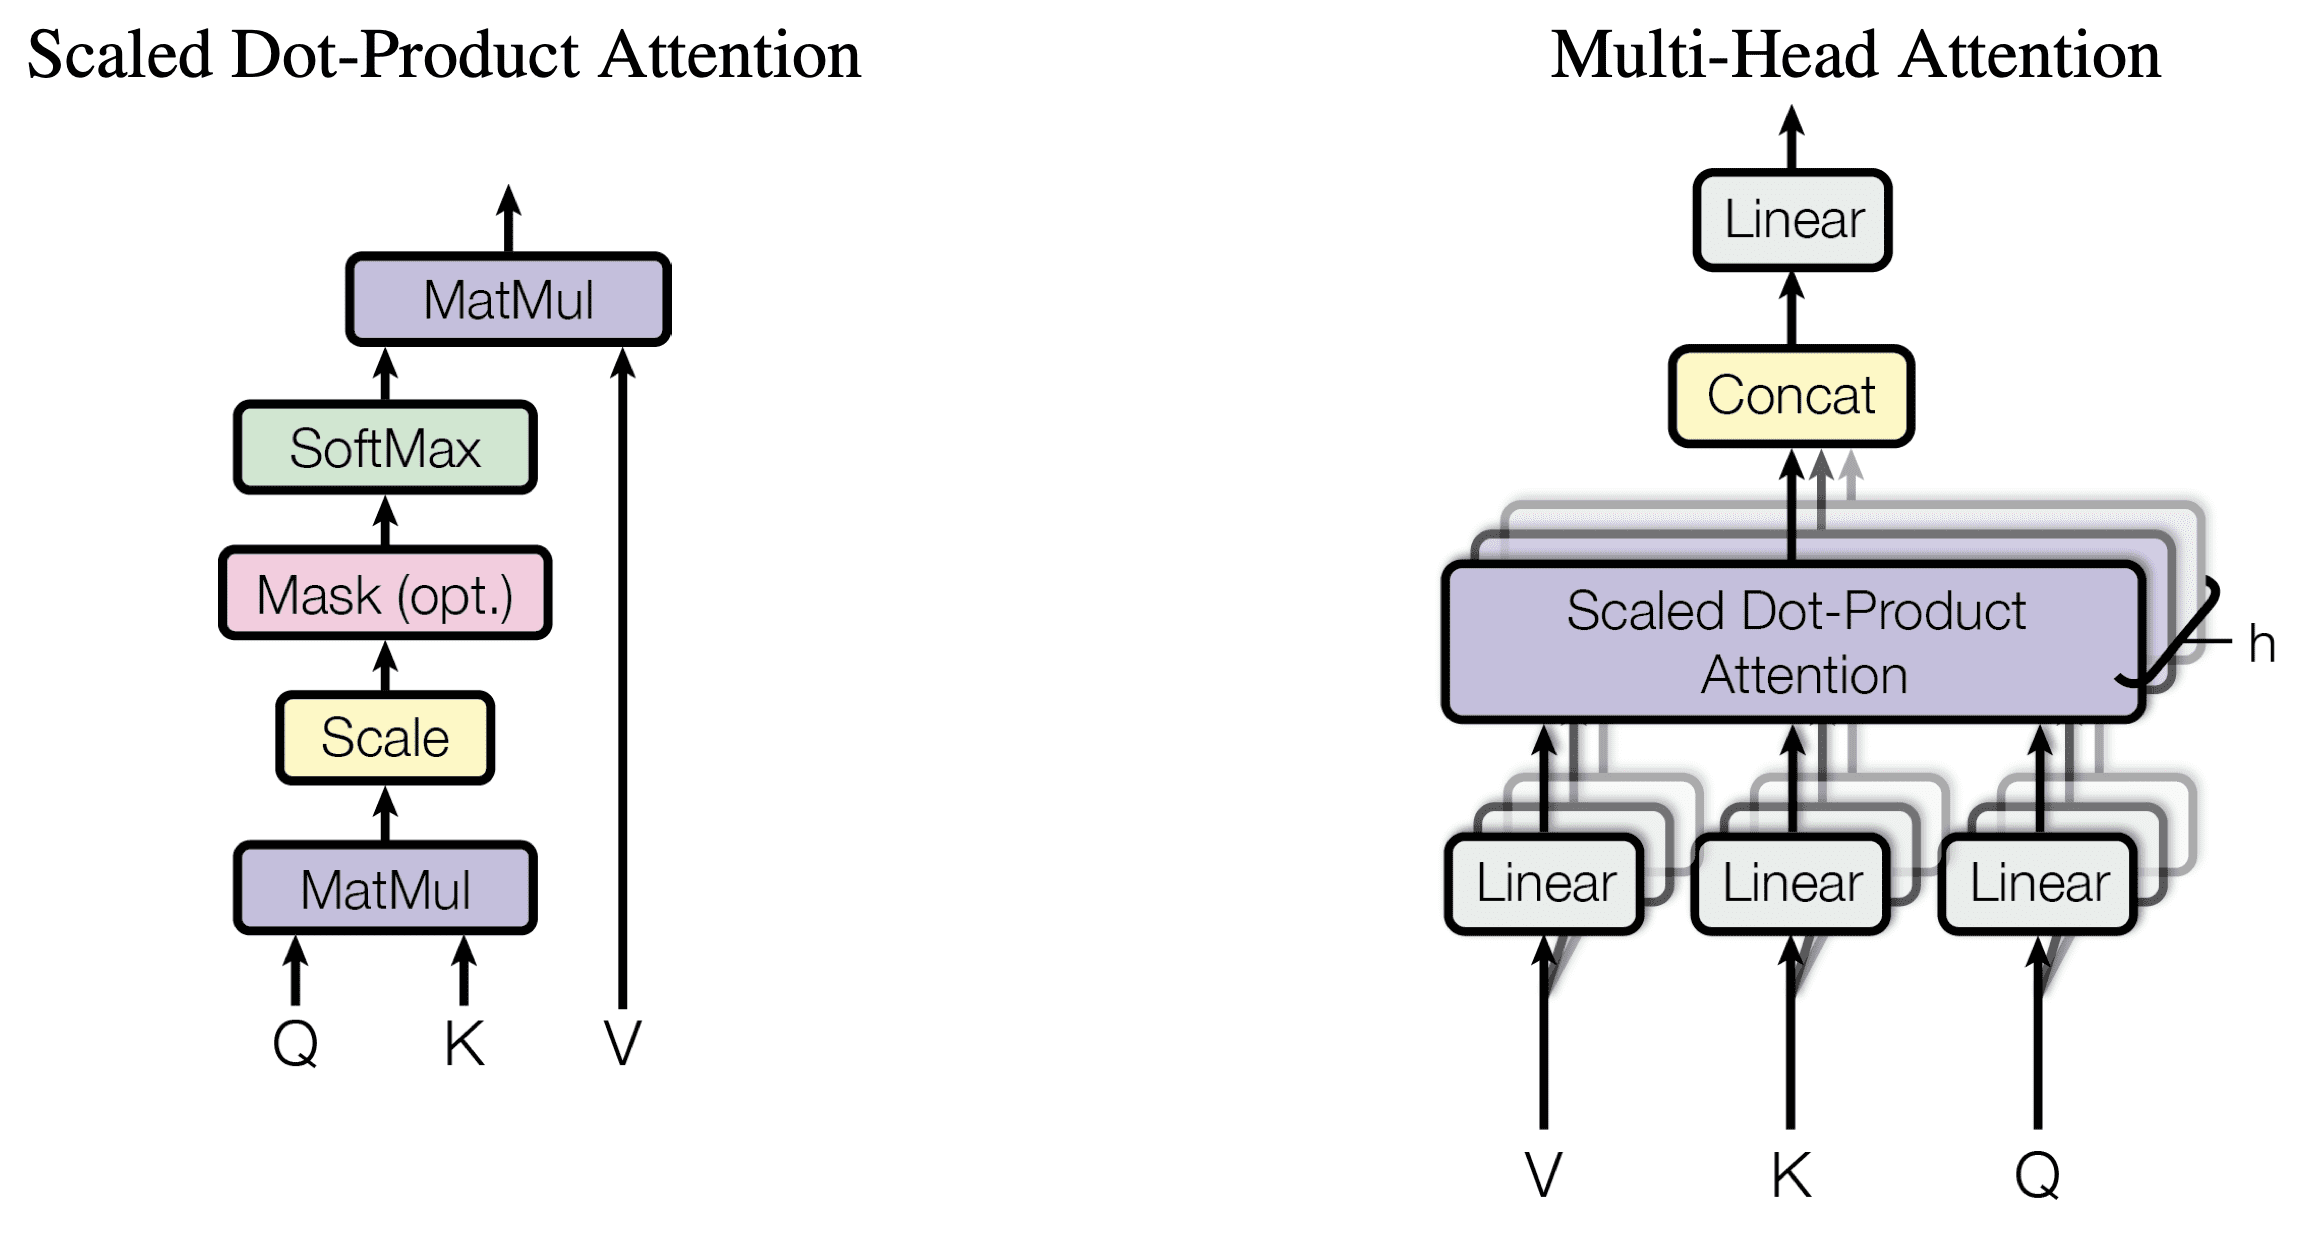
\includegraphics[width=0.6\textwidth]{scaled_dot_product_attention.png}
    \captionof{figure}{Sơ đồ Scaled Dot-Product Attention. Đầu vào là các ma trận Q, K, V và đầu ra là một ma trận đã được làm giàu ngữ cảnh.}
    \label{fig:scaled_dot_product_attention}
\end{center}

\subsubsection{Multi-Head Attention}
\paragraph{Vấn đề của Single-Head Attention}
Chỉ có một bộ Self-Attention duy nhất sẽ bị hạn chế. Nó giống như việc bạn chỉ có thể tập trung vào một khía cạnh của mối quan hệ giữa các từ. Ví dụ, khi xử lý câu "Con mèo ngồi trên chiếu", một "đầu" chú ý (attention head) có thể học cách liên kết "nó" với "mèo" (quan hệ đồng tham chiếu), nhưng có thể sẽ bỏ lỡ các mối quan hệ khác (ví dụ, quan hệ cú pháp).

\paragraph{Giải pháp: Nhiều "đầu" chú ý song song}
Multi-Head Attention giải quyết vấn đề này bằng cách chạy nhiều cơ chế Scaled Dot-Product Attention một cách \textbf{song song}.
\begin{itemize}
    \item Thay vì chỉ có một bộ trọng số $(W^Q, W^K, W^V)$, chúng ta có $h$ bộ (ví dụ, $h=8$).
    \item Mỗi bộ trọng số này $(W^Q_i, W^K_i, W^V_i)$ với $i=1,\dots,h$ được gọi là một "đầu" chú ý.
    \item Mỗi "đầu" sẽ chiếu các vector đầu vào vào một không gian con khác nhau và thực hiện Self-Attention một cách độc lập. Điều này cho phép mỗi đầu có thể học một loại quan hệ khác nhau. Ví dụ, một đầu có thể học quan hệ cú pháp, một đầu khác học quan hệ ngữ nghĩa, một đầu khác học quan hệ đồng tham chiếu...
    \item Các vector đầu ra từ tất cả các đầu sau đó được \textbf{nối lại (concatenated)} với nhau.
    \item Vector nối này sau đó được chiếu qua một ma trận trọng số cuối cùng $W^O$ để tạo ra vector đầu ra cuối cùng của lớp Multi-Head Attention.
\end{itemize}

\begin{center}
    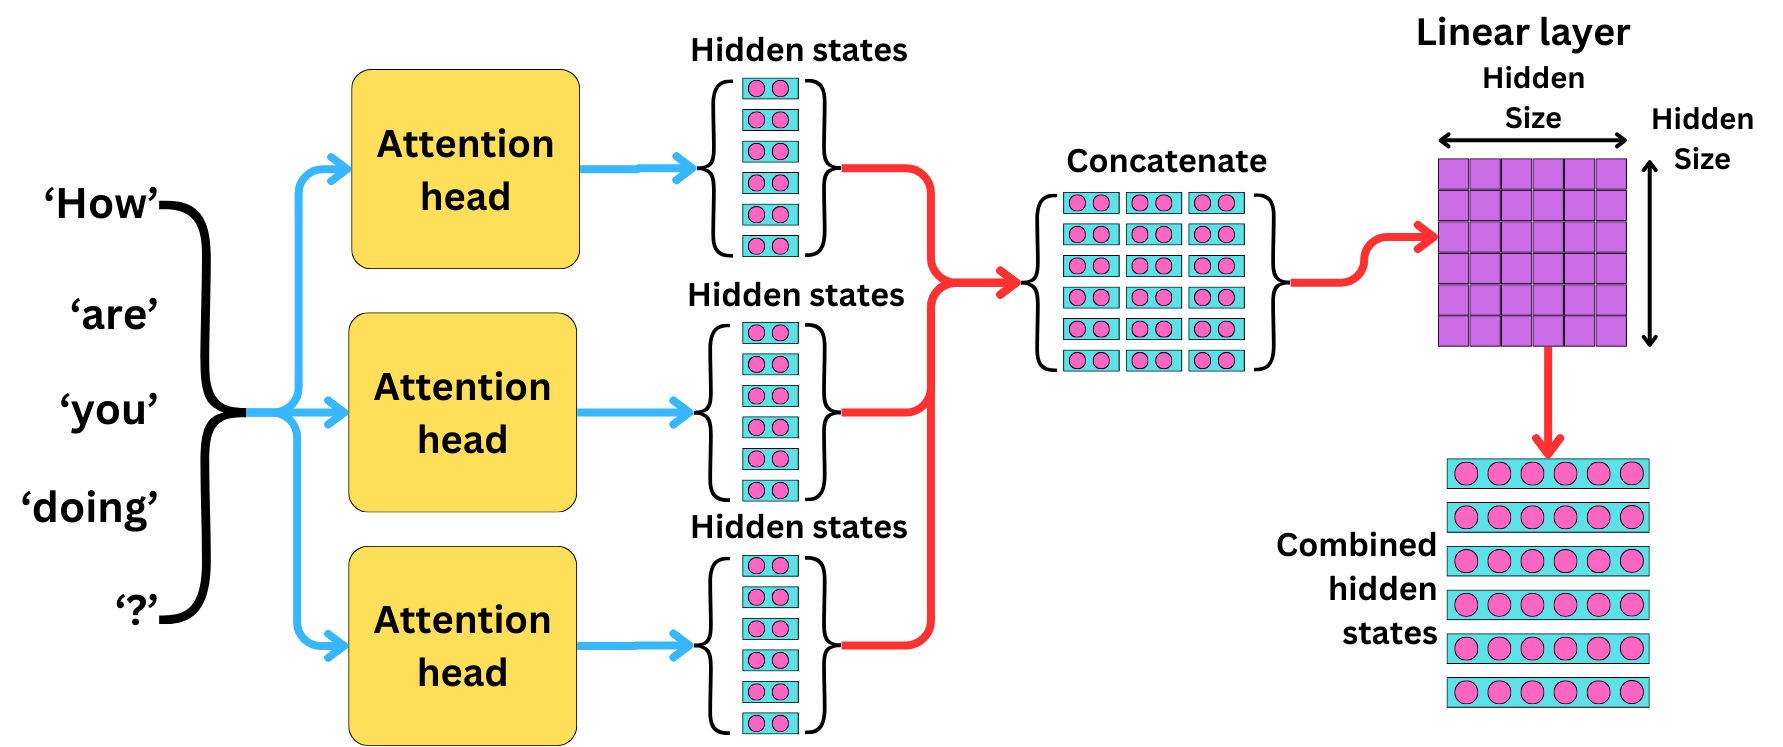
\includegraphics[width=0.8\textwidth]{multi_head_attention.png}
    \captionof{figure}{Kiến trúc Multi-Head Attention, bao gồm nhiều "đầu" Scaled Dot-Product Attention chạy song song.}
    \label{fig:multi_head_attention}
\end{center}

Multi-Head Attention cho phép mô hình cùng lúc chú ý đến thông tin từ các không gian biểu diễn khác nhau tại các vị trí khác nhau. Đây là một trong những nhân tố chính tạo nên sức mạnh biểu diễn của Transformer.

\subsection{Kiến trúc Encoder-Decoder và các thành phần phụ}
\label{ssec:transformer_architecture}
Transformer gốc vẫn giữ kiến trúc Encoder-Decoder của Seq2Seq, nhưng thay thế hoàn toàn các lớp RNN bằng các khối Self-Attention và các lớp Feed-Forward.

\subsubsection{The Encoder Stack}
Encoder của Transformer là một chuỗi gồm $N$ (ví dụ, $N=6$) khối Encoder giống hệt nhau được xếp chồng lên nhau. Mỗi khối bao gồm hai lớp con chính:
\begin{enumerate}
    \item \textbf{Multi-Head Self-Attention Layer:} Lớp này thực hiện Self-Attention trên chuỗi đầu vào.
    \item \textbf{Position-wise Feed-Forward Network (FFN):} Đây là một mạng nơ-ron truyền thẳng đơn giản, bao gồm hai lớp tuyến tính với một hàm kích hoạt ReLU ở giữa.
        $$ \text{FFN}(x) = \max(0, xW_1 + b_1)W_2 + b_2 $$
        FFN này được áp dụng một cách \textbf{độc lập và giống hệt nhau} cho từng vị trí (position) trong chuỗi.
\end{enumerate}
Ngoài ra, mỗi lớp con này còn được bao bọc bởi hai thành phần quan trọng khác:
\begin{itemize}
    \item \textbf{Residual Connection (Kết nối phần dư):} Đầu ra của mỗi lớp con là $\text{LayerNorm}(x + \text{Sublayer}(x))$. Tức là, đầu vào $x$ của lớp con được cộng trực tiếp vào đầu ra của chính lớp đó ($\text{Sublayer}(x)$). Kết nối phần dư này giúp gradient chảy dễ dàng hơn qua các mạng sâu và chống lại vấn đề triệt tiêu gradient.
    \item \textbf{Layer Normalization (Chuẩn hóa lớp):} Chuẩn hóa đầu ra của mỗi lớp con để ổn định quá trình huấn luyện.
\end{itemize}
\begin{tcolorbox}[
    title={Vai trò của các Thành phần Phụ trong Khối Transformer},
    colback=blue!5!white, colframe=blue!50!black, fonttitle=\bfseries
]
Nếu Self-Attention là "bộ não" thì FFN, Residual Connection và Layer Normalization là "hệ tuần hoàn và hệ thần kinh" giúp bộ não đó hoạt động ổn định và hiệu quả.
\begin{itemize}
    \item \textbf{Position-wise Feed-Forward Network (FFN):}
        \begin{itemize}
            \item \textbf{Vai trò:} Lớp Self-Attention chủ yếu thực hiện việc \textbf{trộn thông tin (mixing information)} giữa các từ. Sau bước này, lớp FFN được áp dụng riêng lẻ cho từng vị trí để \textbf{xử lý sâu hơn (deep processing)} thông tin đã được trộn đó. Nó có thể được xem như một bước "biến đổi phi tuyến" mạnh mẽ, giúp mô hình học các mối quan hệ phức tạp hơn, hoặc thậm chí hoạt động như một bộ nhớ key-value đơn giản để lưu trữ các tri thức đã học.
            \item \textbf{Tại sao "Position-wise"?} Việc áp dụng cùng một FFN cho mọi vị trí tương tự như việc chia sẻ trọng số trong RNN hoặc phép tích chập 1x1 trong CNN. Nó đảm bảo tính nhất quán trong cách xử lý ở các vị trí khác nhau.
        \end{itemize}
    \item \textbf{Residual Connection \& Layer Normalization:}
        \begin{itemize}
            \item \textbf{Mục đích kép của Residual Connection:} 1) Nó tạo ra một "con đường tắt" cho gradient, giúp chống lại vấn đề triệt tiêu gradient và cho phép huấn luyện các mô hình rất sâu (ví dụ, hàng chục lớp Transformer). 2) Nó đảm bảo rằng ngay cả khi một lớp con (Sublayer) không học được gì hữu ích, thông tin từ lớp trước đó vẫn có thể đi thẳng tới lớp tiếp theo mà không bị mất mát. Mô hình chỉ cần học phần "thay đổi" (delta) so với đầu vào.
            \item \textbf{Layer Normalization:} Nó giúp ổn định quá trình huấn luyện bằng cách giữ cho đầu ra của mỗi lớp con có phân phối ổn định (trung bình 0, phương sai 1). Điều này làm cho quá trình tối ưu hóa trở nên mượt mà hơn và ít nhạy cảm hơn với việc khởi tạo trọng số. Sự kết hợp của Residuals và Norm là công thức vàng để huấn luyện các mạng nơ-ron rất sâu thành công.
        \end{itemize}
\end{itemize}
\end{tcolorbox}
\subsubsection{The Decoder Stack}
Decoder cũng là một chuỗi gồm $N$ khối Decoder giống hệt nhau. Mỗi khối Decoder có ba lớp con:
\begin{enumerate}
    \item \textbf{Masked Multi-Head Self-Attention Layer:} Tương tự như Self-Attention của Encoder, nhưng có một sự thay đổi quan trọng: \textbf{masking (che giấu)}. Khi dự đoán từ ở vị trí $i$, Decoder chỉ được phép "chú ý" đến các từ ở các vị trí trước đó (từ $1$ đến $i$).
    \begin{itemize}
        \item \textbf{Cơ chế kỹ thuật:} Việc này được thực hiện bằng cách thêm một "ma trận mặt nạ" (mask matrix) vào ma trận điểm chú ý, ngay trước bước softmax. Ma trận này có giá trị là 0 cho các vị trí được phép chú ý và $-\infty$ cho các vị trí bị cấm.
        \item \textbf{Hệ quả:} Sau khi qua hàm softmax, các vị trí có giá trị $-\infty$ sẽ có trọng số chú ý bằng 0, đảm bảo rằng thông tin từ các từ tương lai không bị "rò rỉ" vào quá trình tính toán.
        \item \textbf{Mục đích:} Điều này là để đảm bảo tính \textbf{tự hồi quy (auto-regressive)} của mô hình, ngăn không cho nó "gian lận" bằng cách nhìn vào các từ mà nó đang cố gắng dự đoán. Nó mô phỏng quá trình sinh văn bản trong thực tế, nơi chúng ta chỉ biết những từ đã viết trước đó.
    \end{itemize}
    \item \textbf{Multi-Head Cross-Attention Layer:} Đây là nơi Decoder thực sự tương tác với Encoder, và là nơi kiến trúc "chú ý" của Seq2Seq gốc được tái hiện.
    \begin{itemize}
        \item \textbf{Dòng chảy thông tin:} Ở lớp này, \textbf{Query} được tạo ra từ đầu ra của lớp Masked Self-Attention của Decoder. Nó đại diện cho "câu hỏi" mà Decoder đang muốn hỏi: "Dựa trên những gì tôi đã dịch cho đến nay, tôi nên nhìn vào đâu trong câu gốc để dịch từ tiếp theo?".
        \item Trong khi đó, \textbf{Key và Value} được tạo ra từ \textbf{đầu ra của khối Encoder cuối cùng}. Chúng đại diện cho "kho thông tin" mà Decoder có thể truy vấn.
        \item \textbf{Kết quả:} Lớp này cho phép mỗi từ trong chuỗi đầu ra chú ý đến tất cả các từ trong chuỗi đầu vào, giúp mô hình căn chỉnh (align) các từ giữa hai ngôn ngữ một cách hiệu quả.
    \end{itemize}
    \item \textbf{Position-wise Feed-Forward Network:} Giống hệt như trong Encoder.
\end{enumerate}
Tương tự Encoder, mỗi lớp con của Decoder cũng có Residual Connection và Layer Normalization.

\subsubsection{Huấn luyện và Tối ưu hóa}
\label{sssec:transformer_training}
Kiến trúc Transformer gốc được huấn luyện cho tác vụ dịch máy. Tương tự như mô hình Seq2Seq, mục tiêu là tối thiểu hóa hàm mất mát \textbf{Cross-Entropy} giữa phân phối xác suất đầu ra của Decoder và từ tham chiếu (ground truth).

\begin{itemize}
    \item \textbf{Hàm Mất mát:} Lỗi được tính toán tại mỗi bước sinh từ của Decoder và được tổng hợp lại trên toàn bộ chuỗi.
    \item \textbf{Tối ưu hóa:} Bài báo gốc sử dụng bộ tối ưu hóa \textbf{Adam} \cite{kingma2014adam} với một lịch trình tốc độ học (learning rate schedule) đặc biệt bao gồm một giai đoạn "warmup" (tăng tuyến tính) sau đó là giảm dần theo hàm căn bậc hai nghịch đảo. Lịch trình này được chứng minh là rất quan trọng để huấn luyện Transformer một cách ổn định.
    \item \textbf{Điều chuẩn (Regularization):} Hai kỹ thuật điều chuẩn chính được sử dụng để tránh overfitting là \textbf{Dropout} \cite{srivastava2014dropout}, được áp dụng sau mỗi lớp con (trước kết nối phần dư), và \textbf{Label Smoothing}, một kỹ thuật làm cho các nhãn thật trở nên "mềm" hơn một chút (ví dụ, thay vì [0, 0, 1, 0], nhãn có thể là [0.025, 0.025, 0.9, 0.025]), giúp mô hình bớt tự tin thái quá và tổng quát hóa tốt hơn.
\end{itemize}

\subsection{Positional Encoding: Thêm thông tin về vị trí}
\label{ssec:positional_encoding_intro}

Một vấn đề lớn của việc loại bỏ RNN là chúng ta đã làm mất thông tin về \textbf{thứ tự của các từ}. Self-Attention, về bản chất, không nhạy cảm với vị trí; nếu ta hoán vị các từ trong câu, ma trận chú ý cũng sẽ bị hoán vị tương ứng mà không thay đổi bản chất.

Để giải quyết vấn đề này, Transformer thêm một vector gọi là \textbf{Positional Encoding (Mã hóa Vị trí)} vào các vector embedding đầu vào. Vector này cung cấp thông tin về vị trí tuyệt đối hoặc tương đối của một từ trong chuỗi.

\subsubsection{Absolute Positional Encoding (Sinusoidal)}
Đây là phương pháp được sử dụng trong bài báo gốc. Các vector mã hóa vị trí được tạo ra bằng các hàm sin và cos với các tần số khác nhau:
$$ PE_{(pos, 2i)} = \sin(pos / 10000^{2i/d_{\text{model}}}) $$
$$ PE_{(pos, 2i+1)} = \cos(pos / 10000^{2i/d_{\text{model}}}) $$
Trong đó $pos$ là vị trí của từ, $i$ là chỉ số chiều của vector, và $d_{\text{model}}$ là số chiều của embedding.
\paragraph{Tại sao lại dùng sin và cos?}
\begin{itemize}
    \item \textbf{Giá trị duy nhất:} Mỗi vị trí có một vector mã hóa duy nhất.
    \item \textbf{Mô hình có thể học quan hệ tương đối:} Có một tính chất toán học quan trọng: mã hóa vị trí của $pos+k$ có thể được biểu diễn như một hàm tuyến tính của mã hóa vị trí của $pos$. Điều này cho phép mô hình dễ dàng học cách chú ý đến các vị trí tương đối, ví dụ "từ cách 2 vị trí về bên phải".
    \item \textbf{Khả năng ngoại suy:} Có thể tạo ra vector mã hóa cho các chuỗi dài hơn những chuỗi đã thấy trong quá trình huấn luyện.
\end{itemize}

\subsubsection{Relative Positional Encoding}
Các phương pháp sau này cho rằng thông tin về khoảng cách tương đối ("từ này cách từ kia bao xa?") quan trọng hơn vị trí tuyệt đối. Các phương pháp mã hóa vị trí tương đối sẽ sửa đổi trực tiếp cơ chế Self-Attention, thêm một số hạng biểu diễn cho khoảng cách tương đối vào lúc tính điểm chú ý.

\subsubsection{Rotary Position Embedding (RoPE)}
Đây là một phương pháp mã hóa vị trí tương đối rất thanh lịch và hiệu quả \cite{su2021roformer}, được sử dụng trong nhiều LLM hiện đại như Llama.
\begin{itemize}
    \item \textbf{Ý tưởng:} Thay vì cộng, RoPE \textbf{xoay (rotates)} các vector Query và Key một góc phụ thuộc vào vị trí tuyệt đối của chúng.
    \item \textbf{Hệ quả:} Tích vô hướng giữa hai vector đã được xoay ($q_m^T k_n$) sẽ chỉ phụ thuộc vào vector ban đầu và \textbf{khoảng cách tương đối} giữa chúng ($m-n$), chứ không phụ thuộc vào vị trí tuyệt đối $m, n$.
\end{itemize}
RoPE đã chứng tỏ khả năng ngoại suy độ dài ngữ cảnh rất tốt và là một trong những phương pháp mã hóa vị trí hàng đầu hiện nay.
% % !TEX root = ../main.tex
% File: chapters_part1/chap4_2.tex
% Nội dung cho Chương 4, Phần 2

\section{Phân loại Kiến trúc LLMs}
\label{sec:llm_architectures_classification}

Kiến trúc Transformer gốc mà chúng ta vừa phân tích là một mô hình Encoder-Decoder hoàn chỉnh, được thiết kế cho các tác vụ chuỗi-sang-chuỗi (sequence-to-sequence). Tuy nhiên, các nhà nghiên cứu nhanh chóng nhận ra rằng bằng cách chỉ sử dụng một phần của kiến trúc này -- hoặc chỉ Encoder, hoặc chỉ Decoder -- họ có thể tạo ra các mô hình được chuyên môn hóa cao và cực kỳ hiệu quả cho các loại tác vụ khác nhau.

Sự phân tách này đã khai sinh ra ba "họ" kiến trúc chính, định hình nên toàn bộ bối cảnh của các Mô hình Ngôn ngữ Lớn (LLMs) ngày nay. Hiểu rõ ba họ kiến trúc này là chìa khóa để lựa chọn mô hình phù hợp cho ứng dụng của bạn.

\subsection{Họ Mô hình chỉ Encoder (Encoder-Only): Bậc thầy của Sự Hiểu Ngôn ngữ}
\label{ssec:encoder_only}

Các mô hình thuộc họ này chỉ sử dụng khối Encoder của kiến trúc Transformer. Chúng được thiết kế với một mục tiêu duy nhất: tạo ra các \textbf{biểu diễn ngữ cảnh sâu sắc (deep contextualized representations)} cho văn bản đầu vào.

\begin{tcolorbox}[
    title=Triết lý của Encoder-Only,
    colback=blue!5!white, colframe=blue!75!black, fonttitle=\bfseries
]
"Để thực sự hiểu ý nghĩa của một từ trong câu, tôi cần phải nhìn vào \textbf{cả hai phía}: những từ đứng trước nó và những từ đứng sau nó."
\end{tcolorbox}

\subsubsection{Kiến trúc và Mục tiêu Huấn luyện Nền tảng}
\paragraph{Kiến trúc và Tính hai chiều (Bidirectionality)}
Đây là đặc điểm quan trọng nhất. Nhờ cơ chế Self-Attention không bị che (unmasked), tại mỗi lớp, mỗi từ có thể "chú ý" đến tất cả các từ khác trong câu, cả bên trái và bên phải. Điều này cho phép mô hình xây dựng một sự hiểu biết toàn diện về ngữ cảnh, điều mà các mô hình hồi tiếp (RNN) hay tự hồi quy (Decoder-Only) không thể làm được. Đầu ra của mô hình là một chuỗi các vector embedding, mỗi vector tương ứng với một token đầu vào, nhưng đã được "làm giàu" bởi thông tin ngữ cảnh hai chiều sâu sắc.

\paragraph{Mục tiêu Huấn luyện: Masked Language Modeling (MLM)}
MLM là mục tiêu huấn luyện cốt lõi của BERT và nhiều mô hình kế nhiệm.
\begin{itemize}
    \item \textbf{Cơ chế:} Lấy một câu đầu vào, che (mask) ngẫu nhiên khoảng 15\% số token bằng một token đặc biệt `[MASK]`. Sau đó, nhiệm vụ của mô hình là \textbf{dự đoán các token gốc đã bị che}, dựa vào các token không bị che xung quanh.
    \item \textbf{Tại sao lại hiệu quả?} MLM buộc mô hình phải học các mối quan hệ ngữ nghĩa và cú pháp sâu sắc từ cả hai phía để có thể "điền vào chỗ trống". Nó không chỉ là dự đoán từ tiếp theo, mà là một bài kiểm tra "đọc hiểu" thực sự.
\end{itemize}

\begin{center}
    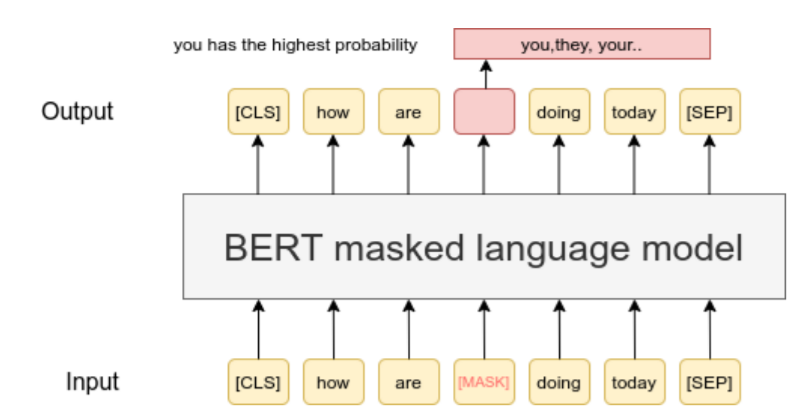
\includegraphics[width=0.8\textwidth]{bert_mlm_nsp.png}
    \captionof{figure}{Mục tiêu huấn luyện kinh điển của BERT: Masked Language Modeling (MLM). Mô hình phải dự đoán các token bị che dựa trên ngữ cảnh hai chiều.}
    \label{fig:bert_mlm_nsp}
\end{center}

\subsubsection{Sự phát triển và các biến thể của Họ Encoder-Only}
Từ nền tảng của BERT, một hệ sinh thái đa dạng các mô hình Encoder-Only đã ra đời, mỗi loại được tối ưu cho các mục đích khác nhau: hiệu suất, kích thước, tác vụ cụ thể, hay miền kiến thức chuyên biệt.

\paragraph{1. Gia đình BERT: Những người kế nhiệm trực tiếp}
Đây là các mô hình cải tiến trực tiếp từ kiến trúc và phương pháp huấn luyện của BERT.
\begin{itemize}
    \item \textbf{RoBERTa (Facebook) \cite{liu2019roberta}:} Không thay đổi kiến trúc, nhưng chứng minh rằng việc tối ưu hóa kỹ lưỡng quá trình huấn luyện có thể mang lại hiệu quả vượt trội. Các cải tiến chính bao gồm: huấn luyện lâu hơn, trên nhiều dữ liệu hơn, với batch size lớn hơn, loại bỏ mục tiêu NSP (Next Sentence Prediction), và sử dụng "che động" (dynamic masking).
    \item \textbf{DistilBERT (Hugging Face) \cite{sanh2019distilbert}:} Một phiên bản "chưng cất" nhỏ hơn, nhanh hơn của BERT. Nó sử dụng kỹ thuật \textit{knowledge distillation}, trong đó một mô hình "học trò" (student) nhỏ hơn học cách bắt chước đầu ra của một mô hình "giáo viên" (teacher) lớn hơn (BERT). DistilBERT giữ lại 97\% hiệu năng của BERT nhưng chỉ có 60\% kích thước.
    \item \textbf{ALBERT (Google) \cite{lan2019albert}:} Một cách tiếp cận khác để giảm tham số. ALBERT sử dụng hai kỹ thuật chính: \textit{factorized embedding parameterization} (phân tách ma trận embedding từ lớn thành hai ma trận nhỏ) và \textit{cross-layer parameter sharing} (chia sẻ trọng số của các khối Transformer với nhau).
    \item \textbf{SpanBERT (Facebook) \cite{joshi2020spanbert}:} Tối ưu hóa BERT cho các tác vụ cần hiểu các \textbf{đoạn văn bản (spans)} liên tục, như Hỏi-đáp trích xuất. Thay vì che các token ngẫu nhiên, SpanBERT che các đoạn ngẫu nhiên và huấn luyện mô hình dự đoán toàn bộ đoạn bị che chỉ từ các token ở biên của đoạn đó.
\end{itemize}

\paragraph{2. Các mô hình Biểu diễn Câu: Chuyên gia về Tìm kiếm Ngữ nghĩa}
Một hạn chế của BERT gốc là nó không tạo ra các vector biểu diễn câu (sentence embeddings) tốt "ngay lập tức". Việc lấy embedding của token `[CLS]` hoặc lấy trung bình các token embedding thường cho kết quả tìm kiếm tương đồng không cao. Nhánh mô hình này giải quyết vấn đề đó.
\begin{itemize}
    \item \textbf{SBERT (Sentence-BERT) \cite{reimers2019sentence}:} Là mô hình tiên phong. SBERT tinh chỉnh BERT trên các cặp câu bằng cách sử dụng kiến trúc \textit{siamese} hoặc \textit{triplet}. Kiến trúc này buộc mô hình phải tạo ra một không gian vector mà ở đó các câu có ngữ nghĩa giống nhau sẽ có vector gần nhau (cosine similarity cao) và ngược lại.
    \item \textbf{SimCSE (Simple Contrastive Sentence Embedding) \cite{gao2021simcse}:} Một phương pháp học tương phản (contrastive learning) đơn giản nhưng cực kỳ hiệu quả. Để tạo một cặp dương, SimCSE chỉ cần đưa cùng một câu qua mô hình BERT hai lần (với dropout khác nhau). Các câu khác trong batch được coi là cặp âm. Kỹ thuật này tạo ra các embedding câu chất lượng rất cao mà không cần dữ liệu gán nhãn.
    \item \textbf{E5 (Embeddings from bidErectional Encoder rEpresentations \cite{wang2022text}), Contriever, etc.:} Là thế hệ mô hình embedding mới nhất, được huấn luyện đặc biệt cho các tác vụ \textbf{tìm kiếm (retrieval)}, đặc biệt là tìm kiếm bất đối xứng (truy vấn ngắn, tài liệu dài). Chúng thường đạt hiệu năng SOTA trên các benchmark tìm kiếm ngữ nghĩa.
\end{itemize}

\paragraph{3. Các mô hình cho Miền chuyên biệt và Đa ngôn ngữ}
Ý tưởng cốt lõi là một mô hình được huấn luyện trước trên dữ liệu chuyên ngành sẽ hiểu thuật ngữ và ngữ cảnh của ngành đó tốt hơn.
\begin{itemize}
    \item \textbf{SciBERT \cite{beltagy2019scibert}, BioBERT \cite{lee2020biobert}, ClinicalBERT \cite{alsentzer2019publicly}:} Được huấn luyện trên các kho văn bản khoa học, y sinh, và y tế lâm sàng.
    \item \textbf{FinBERT:} Chuyên cho lĩnh vực tài chính.
    \item \textbf{LegalBERT:} Chuyên cho lĩnh vực pháp luật.
    \item \textbf{CamemBERT \cite{martin2019camembert} (Pháp), PhoBERT \cite{nguyen2020phobert} (Việt), etc.:} Là các mô hình theo kiến trúc RoBERTa nhưng được huấn luyện từ đầu trên kho dữ liệu lớn của một ngôn ngữ cụ thể, cho hiệu năng vượt trội so với các mô hình đa ngôn ngữ trên ngôn ngữ đó.
\end{itemize}

\paragraph{4. Các Encoder Hiện đại, Gọn nhẹ và Hiệu quả}
Nhánh này tập trung vào việc tạo ra các mô hình nhỏ gọn hơn nhưng vẫn giữ được hiệu năng cao thông qua các cải tiến về kiến trúc và mục tiêu huấn luyện.
\begin{itemize}
    \item \textbf{MiniLM (Microsoft) \cite{wang2020minilm}:} Sử dụng một phương pháp chưng cất tri thức sâu, trong đó mô hình học trò không chỉ bắt chước đầu ra cuối cùng mà còn cả ma trận chú ý và mối quan hệ giữa các vector value từ mô hình giáo viên.
    \item \textbf{DeBERTa (Microsoft) \cite{he2020deberta}:} Một trong những encoder mạnh nhất hiện nay. DeBERTa giới thiệu cơ chế \textit{disentangled attention}, tách rời việc mã hóa nội dung từ và vị trí tương đối của chúng.
    \item \textbf{MPNet (Microsoft) \cite{song2020mpnet}:} Kết hợp τα tốt nhất của cả hai thế giới: MLM (BERT) và Permuted Language Modeling (XLNet). Nó giải quyết sự không tương thích giữa pre-training và fine-tuning, cho phép mô hình học các phụ thuộc hai chiều một cách toàn diện hơn.
\end{itemize}

\paragraph{5. Các Encoder với Mục tiêu Huấn luyện khác MLM}
MLM không phải là cách duy nhất để huấn luyện một encoder hai chiều.
\begin{itemize}
    \item \textbf{ELECTRA (Google) \cite{clark2020electra}:} Sử dụng một tác vụ hiệu quả hơn là \textit{replaced token detection}. Một mô hình "generator" nhỏ sẽ thay thế một số token trong câu, và mô hình "discriminator" (chính là ELECTRA) phải dự đoán xem mỗi token là gốc hay đã bị thay thế. Tác vụ này hiệu quả hơn vì mô hình học từ \textit{tất cả} các token, không chỉ 15% bị che.
    \item \textbf{XLNet (Google/CMU) \cite{yang2019xlnet}:} Một mô hình \textit{tự hồi quy hoán vị (permutation-based autoregressive)}. Nó dự đoán các token trong câu theo một thứ tự ngẫu nhiên. Bằng cách này, nó có thể "nhìn thấy" ngữ cảnh từ cả hai phía (giống BERT) trong khi vẫn giữ được các lợi ích của mô hình tự hồi quy.
\end{itemize}

\begin{tcolorbox}[
    title=Tổng kết: Điểm mạnh và Ứng dụng của Encoder-Only,
    colback=blue!5!white, colframe=blue!75!black, fonttitle=\bfseries
]
\textbf{Nguyên tắc chung:} Sử dụng mô hình Encoder-Only khi tác vụ của bạn đòi hỏi sự \textbf{hiểu sâu sắc về toàn bộ văn bản đầu vào} và đầu ra không phải là một chuỗi văn bản mới, mạch lạc. Chúng là các mô hình \textbf{NLU (Natural Language Understanding)} chứ không phải \textbf{NLG (Natural Language Generation)}.

\textbf{Ứng dụng điển hình:}
\begin{itemize}
    \item \textbf{Phân loại văn bản (Text Classification):} Phân tích cảm xúc, phát hiện chủ đề, kiểm duyệt nội dung (toxic detection). Mô hình cần hiểu toàn bộ câu để đưa ra một nhãn duy nhất.
    \item \textbf{Gán nhãn chuỗi (Token Classification):} Nhận dạng Thực thể Tên (NER), Gán nhãn Từ loại (POS Tagging). Mô hình cần hiểu ngữ cảnh xung quanh mỗi từ để gán nhãn cho nó.
    \item \textbf{Tìm kiếm Ngữ nghĩa (Semantic Search):} Biến các câu/tài liệu thành các vector embedding có ý nghĩa (sử dụng các mô hình như SBERT, E5). Các vector này sau đó được lưu trữ và truy vấn bằng các thuật toán tìm kiếm lân cận gần nhất (ANN).
    \item \textbf{Hỏi-đáp trích xuất (Extractive QA):} Tìm và trích xuất một đoạn văn bản (span) làm câu trả lời từ một văn bản ngữ cảnh cho trước.
    \item \textbf{Retrieval-Augmented Generation (RAG):} Đây là một ứng dụng lai. Giai đoạn \textbf{Retrieval (Truy xuất)} trong RAG sử dụng một mô hình Encoder-Only (như E5) để biến truy vấn của người dùng và các tài liệu trong cơ sở tri thức thành vector, sau đó tìm ra các tài liệu liên quan nhất. Các tài liệu này sau đó mới được đưa cho một mô hình sinh (Decoder-Only) để tạo ra câu trả lời.
\end{itemize}
\end{tcolorbox}

\subsection{Họ Mô hình chỉ Decoder (Decoder-Only): Bậc thầy của Sự Sáng tạo}
\label{ssec:decoder_only}
Đây là họ kiến trúc đang thống trị thế giới AI hiện nay, là nền tảng của các mô hình như ChatGPT, Llama, và Claude. Chúng chỉ sử dụng khối Decoder của kiến trúc Transformer.

\begin{tcolorbox}[
    title=Triết lý của Decoder-Only,
    colback=red!5!white, colframe=red!75!black, fonttitle=\bfseries
]
"Để viết tiếp một câu chuyện, tôi chỉ cần biết những gì đã được viết \textbf{trước đó}. Tôi không được phép nhìn vào tương lai."
\end{tcolorbox}

\subsubsection{Kiến trúc và Mục tiêu Huấn luyện Nền tảng}
\paragraph{Kiến trúc Tự hồi quy (Auto-regressive Architecture)}
\begin{itemize}
    \item \textbf{Cấu tạo:} Một chuỗi các khối Decoder của Transformer xếp chồng lên nhau. Quan trọng là, chúng \textbf{không có Encoder} và do đó cũng \textbf{không có lớp Cross-Attention}.
    \item \textbf{Tính một chiều (Unidirectionality):} Đây là đặc điểm nhận dạng. Chúng sử dụng \textbf{Masked Self-Attention}. Tại mỗi vị trí, một từ chỉ có thể "chú ý" đến chính nó và các từ đứng trước nó. Nó không thể nhìn thấy các từ ở phía sau, đảm bảo rằng việc dự đoán chỉ dựa trên thông tin quá khứ.
    \item \textbf{Dòng chảy:} Mô hình nhận vào một chuỗi các từ (prompt) và nhiệm vụ của nó là dự đoán từ \textbf{tiếp theo có khả năng nhất}. Từ được dự đoán sau đó được nối vào chuỗi đầu vào, và quá trình này lặp lại để sinh ra từ tiếp theo, cứ thế tiếp tục.
\end{itemize}

\paragraph{Mục tiêu Huấn luyện: Causal Language Modeling (CLM)}
Đây là mục tiêu huấn luyện duy nhất và rất đơn giản: \textbf{Dự đoán từ tiếp theo (Next Token Prediction)}.
\begin{itemize}
    \item \textbf{Cơ chế:} Mô hình được cho xem một đoạn văn bản và được huấn luyện để, tại mỗi vị trí, dự đoán từ tiếp theo dựa trên tất cả các từ đã có trước đó.
    \item \textbf{Sức mạnh của Quy mô:} Bằng cách cố gắng dự đoán từ tiếp theo trên một kho văn bản khổng lồ (hàng nghìn tỷ từ), mô hình buộc phải học một lượng kiến thức khổng lồ về thế giới, về ngữ pháp, ngữ nghĩa, và các mẫu hình lý luận để có thể đưa ra dự đoán tốt. Đây là nền tảng cho các "khả năng nổi trội" (emergent abilities) của LLMs.
\end{itemize}

\begin{center}
    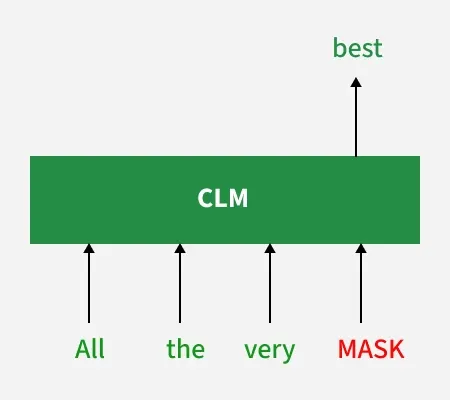
\includegraphics[width=0.8\textwidth]{gpt_clm.png}
    \captionof{figure}{Mục tiêu huấn luyện của GPT: Causal Language Modeling. Tại mỗi bước, mô hình cố gắng dự đoán từ tiếp theo dựa trên các từ trước đó.}
    \label{fig:gpt_clm}
\end{center}

\subsubsection{Sự phát triển và các mô hình tiêu biểu}
Họ mô hình này đã chứng kiến sự phát triển bùng nổ, từ các mô hình tiên phong đến một hệ sinh thái đa dạng các LLMs mã nguồn mở và đóng.

\paragraph{1. Gia đình GPT (OpenAI): Những người tiên phong và dẫn đầu}
Họ mô hình GPT của OpenAI không chỉ định hình nên kiến trúc Decoder-Only mà còn liên tục đẩy lùi các giới hạn của AI.
\begin{itemize}
    \item \textbf{GPT (2018) \cite{radford2018improving}:} Bài báo gốc chứng minh rằng một mô hình Transformer chỉ-Decoder được huấn luyện trước có thể được tinh chỉnh hiệu quả cho các tác vụ NLU.
    \item \textbf{GPT-2 (2019) \cite{radford2019language}:} Gây tiếng vang lớn khi cho thấy việc tăng quy mô (lên tới 1.5 tỷ tham số) có thể tạo ra một mô hình có khả năng sinh văn bản mạch lạc đáng kinh ngạc mà không cần tinh chỉnh (zero-shot).
    \item \textbf{GPT-3 (2020) \cite{brown2020language}:} Mở ra kỷ nguyên LLM thực sự với 175 tỷ tham số. GPT-3 lần đầu tiên thể hiện rõ các \textbf{khả năng nổi trội (emergent abilities)}, đặc biệt là \textbf{học trong ngữ cảnh (in-context learning)}, cho phép nó thực hiện các tác vụ chỉ bằng cách cung cấp vài ví dụ trong prompt (few-shot).
    \item \textbf{InstructGPT \& ChatGPT \cite{ouyang2022training}:} Đánh dấu một bước ngoặt từ "mô hình ngôn ngữ" sang "trợ lý AI" bằng cách sử dụng các kỹ thuật căn chỉnh (alignment) như \textbf{Instruction Tuning} và \textbf{RLHF} (Reinforcement Learning from Human Feedback) để làm cho mô hình hữu ích, trung thực và an toàn hơn.
    \item \textbf{GPT-4 \& GPT-4o (2023-2024) \cite{openai2023gpt4, openai2024gpt4o}:} Là các mô hình SOTA hiện tại, không chỉ mạnh mẽ hơn về ngôn ngữ mà còn trở thành các mô hình \textbf{đa phương thức (multimodal)}, có khả năng hiểu và xử lý cả văn bản, hình ảnh, và âm thanh.
\end{itemize}

\paragraph{2. Làn sóng LLMs Mã nguồn mở và các đối thủ cạnh tranh}
Sự thành công của GPT đã thúc đẩy một làn sóng nghiên cứu và phát triển LLMs trên toàn thế giới, với nhiều mô hình mã nguồn mở mạnh mẽ.
\begin{itemize}
    \item \textbf{LLaMA (Meta) \cite{touvron2023llama}:} Họ mô hình LLaMA (và các phiên bản kế nhiệm LLaMA 2, LLaMA 3) đã "dân chủ hóa" LLMs, cung cấp các mô hình mã nguồn mở có hiệu năng cực kỳ cạnh tranh, tạo điều kiện cho một hệ sinh thái ứng dụng và nghiên cứu khổng lồ.
    \item \textbf{Mistral (Pháp):} Nổi lên như một đối thủ đáng gờm với các mô hình hiệu năng cao nhưng kích thước nhỏ gọn (ví dụ: Mistral 7B \cite{jiang2023mistral}). Họ cũng đi tiên phong trong việc thương mại hóa kiến trúc \textbf{Mixture of Experts (MoE)} với mô hình Mixtral, giúp tăng đáng kể số lượng tham số mà không tăng chi phí suy luận tương ứng.
    \item \textbf{Claude (Anthropic):} Được biết đến với "cửa sổ ngữ cảnh" (context window) rất lớn và tập trung mạnh vào sự an toàn thông qua phương pháp \textbf{Constitutional AI} \cite{bai2022constitutional}.
    \item \textbf{Các mô hình đáng chú ý khác:}
        \begin{itemize}
            \item \textbf{Google:} Gemma (mã nguồn mở), Gemini (mô hình SOTA cạnh tranh với GPT-4).
            \item \textbf{Cohere:} Command R(+), tập trung vào các ứng dụng doanh nghiệp và Retrieval-Augmented Generation (RAG).
            \item \textbf{Các mô hình từ Trung Quốc:} Qwen (Alibaba), Yi, Baichuan, InternLM, DeepSeek, thể hiện sự tiến bộ nhanh chóng của cộng đồng AI Trung Quốc.
            \item \textbf{TII (UAE):} Falcon.
        \end{itemize}
\end{itemize}

\paragraph{3. Các mô hình Decoder-Only chuyên biệt}
Bên cạnh các LLM đa dụng, nhiều mô hình được huấn luyện đặc biệt cho các miền cụ thể.
\begin{itemize}
    \item \textbf{Code LLMs:} Các mô hình được huấn luyện chủ yếu trên dữ liệu mã nguồn để hỗ trợ lập trình. Ví dụ: Codex \cite{chen2021evaluating} (nền tảng của GitHub Copilot đời đầu), StarCoder\cite{li2023starcoder}, CodeLLaMA \cite{roziere2023code}, Phi-3 (Microsoft).
    \item \textbf{Dialogue-focused Models:} Các mô hình được tinh chỉnh đặc biệt cho các tác vụ hội thoại, là tiền thân của các chatbot hiện đại. Ví dụ: DialoGPT (Microsoft) \cite{zhang2019dialogpt}, ChatGLM (Trung Quốc).
\end{itemize}

\begin{tcolorbox}[
    title=Tổng kết: Điểm mạnh và Ứng dụng của Decoder-Only,
    colback=red!5!white, colframe=red!75!black, fonttitle=\bfseries
]
\textbf{Nguyên tắc chung:} Sử dụng mô hình Decoder-Only khi tác vụ của bạn đòi hỏi việc \textbf{sinh ra một chuỗi văn bản mới, mạch lạc, và có tính sáng tạo} dựa trên một ngữ cảnh đầu vào. Chúng là các mô hình \textbf{NLG (Natural Language Generation)} và là nền tảng của AI tạo sinh (Generative AI).

\textbf{Điểm mạnh:}
\begin{itemize}
    \item \textbf{Khả năng sinh văn bản xuất sắc:} Là kiến trúc tốt nhất cho mọi tác vụ NLG.
    \item \textbf{Tính linh hoạt (Zero-shot/Few-shot):} Các mô hình lớn có thể thực hiện nhiều tác vụ chỉ thông qua prompt mà không cần fine-tuning, rất linh hoạt và tiết kiệm chi phí gán nhãn.
\end{itemize}
\textbf{Điểm yếu:}
\begin{itemize}
    \item \textbf{Hiểu ngữ cảnh không sâu bằng Encoder-Only:} Do bản chất một chiều, biểu diễn của một từ không được "nhìn thấy" các từ phía sau. Điều này làm chúng kém tối ưu hơn cho các tác vụ NLU thuần túy so với BERT/RoBERTa.
    \item \textbf{Dễ "ảo giác" (Hallucination):} Có xu hướng bịa đặt thông tin một cách tự tin.
    \item \textbf{Quá trình sinh tuần tự là chậm.}
\end{itemize}

\textbf{Ứng dụng điển hình:}
\begin{itemize}
    \item \textbf{Hệ thống Đối thoại và Trợ lý ảo (Chatbots):} ChatGPT, Claude, Gemini.
    \item \textbf{Sáng tạo nội dung:} Viết văn, làm thơ, soạn email, tóm tắt văn bản (abstractive summarization).
    \item \textbf{Lập trình và Sinh mã (Code Generation):} GitHub Copilot.
    \item \textbf{Giải quyết vấn đề thông qua Prompting:} Bất kỳ tác vụ nào có thể được định dạng dưới dạng "đầu vào -> đầu ra văn bản", từ dịch máy, trả lời câu hỏi, đến lý luận toán học.
\end{itemize}
\end{tcolorbox}


\subsection{Họ Mô hình Encoder-Decoder: Sự kết hợp của hai thế giới}
\label{ssec:encoder_decoder_models}
Họ mô hình này quay trở lại với kiến trúc Transformer gốc ("Attention is All You Need"), sử dụng cả hai thành phần Encoder và Decoder. Mặc dù không còn là tâm điểm chú ý như các LLM Decoder-Only, chúng vẫn là kiến trúc mạnh mẽ và phù hợp nhất cho nhiều tác vụ chuỗi-sang-chuỗi quan trọng.

\begin{tcolorbox}[
    title=Triết lý của Encoder-Decoder,
    colback=green!5!white, colframe=green!60!black, fonttitle=\bfseries
]
"Tôi sẽ dùng một bộ mã hóa hai chiều mạnh mẽ để \textbf{hiểu trọn vẹn} văn bản nguồn, và sau đó dùng một bộ giải mã tự hồi quy để \textbf{sinh ra} văn bản đích dựa trên sự hiểu biết đó."
\end{tcolorbox}

\subsubsection{Kiến trúc và Lợi thế Cốt lõi}
\begin{itemize}
    \item \textbf{Kiến trúc:} Một Encoder hai chiều (giống BERT) để đọc và hiểu toàn bộ chuỗi đầu vào. Một Decoder một chiều (giống GPT) để sinh ra chuỗi đầu ra. Hai thành phần này được kết nối với nhau thông qua cơ chế \textbf{Cross-Attention}, cho phép Decoder "tham khảo" bất kỳ phần nào của chuỗi đầu vào đã được mã hóa ở mỗi bước sinh từ.
    \item \textbf{Lợi thế Cốt lõi:} Sự phân tách vai trò này là một lợi thế không thể thay thế trong các tác vụ đòi hỏi sự hiểu biết sâu sắc về toàn bộ ngữ cảnh nguồn trước khi tạo ra đầu ra. Encoder có thể xây dựng một biểu diễn hai chiều hoàn chỉnh, nắm bắt các mối quan hệ phức tạp trong văn bản nguồn. Decoder sau đó có thể tận dụng biểu diễn phong phú này để tạo ra một đầu ra chính xác và phù hợp hơn.
\end{itemize}

\subsubsection{Sự phát triển và các mô hình tiêu biểu}
Họ Encoder-Decoder có một lịch sử phát triển phong phú, từ mô hình nền tảng đến các biến thể được tối ưu hóa cao cho các tác vụ chuyên biệt.

\paragraph{1. Các mô hình Nền tảng và Đa ngôn ngữ}
\begin{itemize}
    \item \textbf{Transformer (Google, 2017) \cite{vaswani2017attention}:} Bài báo "Attention Is All You Need" chính là khởi nguồn của tất cả. Nó giới thiệu kiến trúc Encoder-Decoder với Self-Attention và đã thay thế hoàn toàn RNN trong các tác vụ dịch máy SOTA thời bấy giờ.
    \item \textbf{T5 (Google, 2019) \cite{raffel2020exploring}:} Phổ biến hóa khung làm việc "Text-to-Text", đối xử mọi bài toán NLP như một tác vụ Seq2Seq, giúp đơn giản hóa và thống nhất quá trình nghiên cứu và ứng dụng.
    \item \textbf{BART (Facebook, 2019) \cite{lewis2019bart}:} Kết hợp các ý tưởng từ BERT (encoder hai chiều) và GPT (decoder tự hồi quy) với mục tiêu huấn luyện khử nhiễu linh hoạt, đặc biệt mạnh mẽ cho các tác vụ sinh văn bản có điều kiện.
    \item \textbf{Các phiên bản Đa ngôn ngữ:} Thành công của các mô hình trên đã dẫn đến các phiên bản đa ngôn ngữ được huấn luyện trên hàng trăm thứ tiếng, bao gồm \textbf{mT5}, \textbf{mBART}, và \textbf{MarianMT} (một mô hình từ Microsoft/Facebook được tối ưu hóa cao cho dịch máy). Gần đây nhất, \textbf{NLLB (No Language Left Behind) \cite{costa2022no}} của Meta đã đẩy giới hạn này đi xa hơn, tập trung vào các ngôn ngữ ít tài nguyên.
\end{itemize}

\paragraph{2. Các biến thể với Mục tiêu Huấn luyện và Kiến trúc Sáng tạo}
Nhiều mô hình đã cải tiến kiến trúc hoặc mục tiêu huấn luyện để đạt hiệu năng vượt trội trên các tác vụ cụ thể, đặc biệt là tóm tắt văn bản.
\begin{itemize}
    \item \textbf{PEGASUS (Google, 2020) \cite{zhang2020pegasus}:} Một mô hình cực kỳ mạnh mẽ cho tóm tắt văn bản. Thay vì che các token (MLM) hay các đoạn (T5), PEGASUS có mục tiêu huấn luyện trước là \textbf{"Gap-Sentences Generation"}. Nó che đi toàn bộ các câu quan trọng trong một tài liệu và yêu cầu mô hình sinh lại các câu đó từ phần còn lại. Điều này mô phỏng rất gần với tác vụ tóm tắt.
    \item \textbf{ProphetNet (Microsoft, 2020) \cite{qi2020prophetnet}:} Cải tiến kiến trúc Decoder để có thể dự đoán \textbf{nhiều bước trong tương lai (future n-gram prediction)} thay vì chỉ một từ tiếp theo. Việc "nhìn xa" này giúp mô hình tránh bị lặp lại và tạo ra các bản tóm tắt chất lượng cao hơn.
    \item \textbf{BERT2BERT \cite{rothe2020leveraging}:} Một kiến trúc đơn giản nhưng hiệu quả, khởi tạo cả Encoder và Decoder bằng các trọng số của một mô hình BERT đã được huấn luyện trước. Đây là một cách "khởi động nóng" (warm-start) hiệu quả cho các tác vụ Seq2Seq như tóm tắt.
    \item \textbf{ByT5 (Google) \cite{xue2022byt5}:} Một biến thể của T5 xử lý trực tiếp \textbf{chuỗi các byte UTF-8} thay vì các token. Cách tiếp cận này loại bỏ sự phức tạp và các lỗi tiềm ẩn của quá trình tokenization, giúp mô hình trở nên mạnh mẽ hơn với nhiễu và đa ngôn ngữ.
\end{itemize}

\paragraph{3. Hướng tới sự Hợp nhất và Linh hoạt}
Các nghiên cứu gần đây tìm cách tạo ra các mô hình linh hoạt hơn, có thể đảm nhận nhiều vai trò khác nhau.
\begin{itemize}
    \item \textbf{UL2 (Google, 2022) \cite{tay2022unifying}:} Giới thiệu một khung làm việc huấn luyện trước \textbf{hợp nhất (unified)}. Bằng cách thay đổi các mục tiêu khử nhiễu, UL2 có thể được huấn luyện để hoạt động như một Encoder-Only, Decoder-Only, hoặc Encoder-Decoder, mở ra hướng đi cho các mô hình đa năng.
    \item \textbf{Flan-T5 (Google):} Là một phiên bản của T5 đã được \textbf{tinh chỉnh theo chỉ dẫn (instruction-tuned) \cite{chung2022scaling}} trên hàng trăm tác vụ NLP được định dạng lại. Quá trình này giúp Flan-T5 có khả năng tổng quát hóa zero-shot đáng kinh ngạc cho các tác vụ mới, một khả năng vốn thường thấy ở các mô hình Decoder-Only. \textbf{Tk-Instruct} cũng là một mô hình tương tự được huấn luyện trên một bộ chỉ dẫn còn lớn hơn.
\end{itemize}

\subsubsection{Khi nào nên sử dụng Họ mô hình Encoder-Decoder?}
\begin{tcolorbox}[
    title=Đánh giá Họ Mô hình Encoder-Decoder,
    colback=green!5!white, colframe=green!60!black, fonttitle=\bfseries
]
\textbf{Nguyên tắc chung:} Sử dụng mô hình Encoder-Decoder khi tác vụ của bạn là một bài toán \textbf{chuỗi-sang-chuỗi (sequence-to-sequence) có điều kiện mạnh mẽ}, nơi chất lượng của đầu ra phụ thuộc rất nhiều vào sự hiểu biết sâu sắc và toàn diện về toàn bộ chuỗi đầu vào.

\textbf{Điểm mạnh:}
\begin{itemize}
    \item \textbf{Hiệu năng SOTA cho các tác vụ Seq2Seq cổ điển:} Là lựa chọn tự nhiên và thường là tốt nhất cho các tác vụ như dịch máy và tóm tắt văn bản, đặc biệt khi cần độ chính xác cao.
    \item \textbf{Kiểm soát tốt hơn:} Việc tách biệt Encoder và Decoder cho phép kiểm soát tốt hơn quá trình mã hóa thông tin nguồn trước khi sinh ra thông tin đích.
\end{itemize}
\textbf{Điểm yếu:}
\begin{itemize}
    \item \textbf{Phức tạp và nhiều tham số hơn:} Phải huấn luyện cả Encoder và Decoder, làm tăng chi phí tính toán và bộ nhớ.
    \item \textbf{Kém linh hoạt trong các tác vụ zero-shot:} So với các mô hình Decoder-Only lớn, chúng thường không có khả năng "học trong ngữ cảnh" (in-context learning) mạnh mẽ và đòi hỏi phải được tinh chỉnh (fine-tuned) cho từng tác vụ cụ thể (ngoại trừ các phiên bản instruction-tuned như Flan-T5).
\end{itemize}
\textbf{Ứng dụng điển hình:}
\begin{itemize}
    \item \textbf{Dịch máy (Machine Translation).}
    \item \textbf{Tóm tắt văn bản (Summarization).}
    \item \textbf{Hỏi-đáp sinh (Generative Question Answering).}
    \item \textbf{Chuyển đổi Dữ liệu-thành-Văn bản (Data-to-text),} ví dụ, sinh mô tả từ một bảng dữ liệu có cấu trúc.
    \item \textbf{Các tác vụ chỉnh sửa văn bản (Text Editing) và tái cấu trúc câu.}
\end{itemize}
\end{tcolorbox}
% % !TEX root = ../main.tex
% File: chapters_part1/chap4_3.tex
% Nội dung cho Chương 4, Phần 3

\section{Các Kỹ thuật Tokenization Hiện đại}
\label{sec:modern_tokenization}

Trước khi một mô hình Transformer có thể xử lý văn bản, văn bản đó phải được chuyển đổi thành một chuỗi các số nguyên, mỗi số đại diện cho một "token" trong từ vựng của mô hình. Quá trình chia một chuỗi văn bản thô thành các token này được gọi là \textbf{tokenization}.

Lựa chọn tokenizer không phải là một quyết định tầm thường. Nó ảnh hưởng trực tiếp đến:
\begin{itemize}
    \item \textbf{Kích thước từ vựng (Vocabulary Size):} Ảnh hưởng đến kích thước của ma trận embedding và lớp softmax cuối cùng.
    \item \textbf{Độ dài chuỗi (Sequence Length):} Ảnh hưởng đến chi phí tính toán và bộ nhớ.
    \item \textbf{Khả năng xử lý từ hiếm và từ OOV (Out-of-Vocabulary):} Một trong những thách thức lớn nhất.
\end{itemize}

Các phương pháp tokenization đơn giản như tách từ theo khoảng trắng hoặc theo quy tắc sẽ tạo ra một từ vựng khổng lồ và không thể xử lý các từ mới, từ ghép, hay lỗi chính tả. Để giải quyết vấn đề này, các mô hình ngôn ngữ lớn hiện đại đều sử dụng các thuật toán tokenization dựa trên \textbf{subword (dưới từ)}.

\begin{tcolorbox}[
    title=Triết lý của Subword Tokenization,
    colback=yellow!10!white, colframe=yellow!50!black, fonttitle=\bfseries
]
Ý tưởng cốt lõi là: các từ phức tạp hoặc hiếm có thể được phân rã thành các đơn vị con (subwords) có ý nghĩa và thường xuyên xuất hiện hơn. Bằng cách này, mô hình có thể hiểu và xử lý bất kỳ từ nào, ngay cả những từ chưa từng thấy, bằng cách tổ hợp các subword mà nó đã biết.
\end{tcolorbox}
\begin{tcolorbox}[
    title={Subword có phải là Hình vị (Morpheme) không?},
    colback=blue!5!white, colframe=blue!75!black, fonttitle=\bfseries
]
Các subword được tạo ra bởi các thuật toán thống kê (như `re`, `play`, `ing` trong `replaying`) thường trùng khớp một cách đáng ngạc nhiên với các hình vị (morphemes) -- các đơn vị ngôn ngữ nhỏ nhất có ý nghĩa.
\begin{itemize}
    \item \textbf{Tại sao có sự trùng khớp?} Bởi vì các hình vị (tiền tố, hậu tố, gốc từ) xuất hiện lặp đi lặp lại trong nhiều từ khác nhau. Các thuật toán như BPE/WordPiece, vốn được thiết kế để tìm các chuỗi con xuất hiện thường xuyên, sẽ tự động "khám phá" ra các hình vị này một cách tự nhiên mà không cần bất kỳ kiến thức ngôn ngữ học nào.
    \item \textbf{Nhưng chúng không hoàn toàn giống nhau.} Các thuật toán này hoàn toàn dựa trên thống kê. Đôi khi chúng có thể tạo ra các subword không có ý nghĩa về mặt ngôn ngữ học (ví dụ: `to`, `ken`, `ization` thay vì `token`, `ization`) nếu sự phân chia đó phổ biến hơn trong kho văn bản.
\end{itemize}
Do đó, có thể nói rằng các tokenizer subword học được một \textbf{sự xấp xỉ dựa trên dữ liệu (data-driven approximation)} của hình thái học ngôn ngữ.
\end{tcolorbox}
Ví dụ, từ ``tokenization'' có thể được chia thành các subword như \texttt{token} và \texttt{\#\#ization}. 
Từ ``hugging'' có thể được chia thành \texttt{hug} và \texttt{\#\#ging}. 
Dấu \texttt{\#\#} (hoặc một ký hiệu đặc biệt khác) cho biết đây là một phần tiếp nối của một từ.

Ba thuật toán subword tokenization chính được sử dụng trong các LLM hiện đại là BPE, WordPiece, và SentencePiece.

\subsection{Byte-Pair Encoding (BPE)}
\label{ssec:bpe}

BPE ban đầu là một thuật toán nén dữ liệu, sau đó được Sennrich và các cộng sự (2015) \cite{sennrich2015neural} điều chỉnh cho NLP. Đây là thuật toán nền tảng cho GPT và nhiều mô hình khác.

\subsubsection{Cơ chế hoạt động: Gộp từ dưới lên (Bottom-up Merging)}
BPE hoạt động theo một quy trình lặp đi lặp lại rất trực quan: \textbf{tìm cặp token liền kề xuất hiện thường xuyên nhất trong kho văn bản và gộp chúng lại thành một token mới}.

\paragraph{Bước 1: Chuẩn bị kho văn bản và Từ vựng ban đầu}
\begin{enumerate}
    \item \textbf{Tiền xử lý:} Lấy một kho văn bản lớn (corpus).
    \item \textbf{Tách từ:} Tách kho văn bản thành các từ, thường theo khoảng trắng. Thống kê tần suất của mỗi từ.
    \item \textbf{Phân rã thành ký tự:} Tách mỗi từ thành một chuỗi các ký tự. Thêm một ký hiệu kết thúc từ đặc biệt (ví dụ: `</w>`) vào cuối mỗi từ. Điều này giúp mô hình biết được ranh giới của từ gốc. Ví dụ: từ "học" có tần suất 5 lần sẽ trở thành `('h', 'ọ', 'c', '</w>') : 5`.
    \item \textbf{Từ vựng ban đầu:} Từ vựng ban đầu bao gồm tất cả các ký tự đơn lẻ xuất hiện trong kho văn bản.
\end{enumerate}

\paragraph{Bước 2: Học các quy tắc gộp (Learn Merges)}
Lặp lại một số lần định trước (ví dụ: 30,000 lần), mỗi lần lặp thực hiện:
\begin{enumerate}
    \item \textbf{Tìm cặp phổ biến nhất:} Duyệt qua toàn bộ kho văn bản (đã được tách thành ký tự) và tìm ra cặp ký tự/token liền kề nào có tần suất xuất hiện cao nhất.
    \item \textbf{Gộp cặp:} Gộp cặp đó lại thành một token mới.
    \item \textbf{Thêm vào từ vựng:} Thêm token mới này vào từ vựng.
    \item \textbf{Cập nhật kho văn bản:} Thay thế tất cả các lần xuất hiện của cặp đã gộp trong kho văn bản bằng token mới.
\end{enumerate}

\begin{example}{Minh họa quá trình học BPE}{ex:bpe_learning}
    Giả sử kho văn bản của chúng ta sau khi tiền xử lý có dạng:
    `{ ('h', 'ọ', 'c', '</w>'): 5, ('đ', 'ọ', 'c', '</w>'): 3, ('h', 'ỏ', 'i', '</w>'): 4 }`

    \textbf{Từ vựng ban đầu:} `{h, ọ, c, </w>, đ, ỏ, i}`
    
    \textbf{Lần lặp 1:}
    \begin{itemize}
        \item Cặp `(ọ, c)` xuất hiện trong "học" (5 lần) và "đọc" (3 lần). Tổng cộng 8 lần. Đây là cặp phổ biến nhất.
        \item \textbf{Gộp:} `(ọ, c)` $\rightarrow$ `ọc`
        \item \textbf{Từ vựng mới:} `{..., ọc}`
        \item \textbf{Cập nhật kho văn bản:} `{ ('h', 'ọc', '</w>'): 5, ('đ', 'ọc', '</w>'): 3, ('h', 'ỏ', 'i', '</w>'): 4 }`
    \end{itemize}

    \textbf{Lần lặp 2:}
    \begin{itemize}
        \item Cặp `(h, ọc)` xuất hiện 5 lần. Cặp `(ọc, </w>)` xuất hiện 8 lần. Cặp `(đ, ọc)` xuất hiện 3 lần... Cặp `(ọc, </w>)` là phổ biến nhất.
        \item \textbf{Gộp:} `(ọc, </w>)` $\rightarrow$ `ọc</w>`
        \item \textbf{Từ vựng mới:} `{..., ọc, ọc</w>}`
        \item \textbf{Cập nhật kho văn bản:} `{ ('h', 'ọc</w>'): 5, ('đ', 'ọc</w>'): 3, ('h', 'ỏ', 'i', '</w>'): 4 }`
    \end{itemize}
    
    Quá trình này tiếp tục. Cuối cùng, từ vựng sẽ chứa các token từ các ký tự đơn lẻ (`h`, `i`, ...), các subword phổ biến (`ọc`, `ọc</w>`), và có thể cả các từ hoàn chỉnh nếu chúng đủ phổ biến (`học</w>`).
\end{example}

\paragraph{Bước 3: Tokenize một câu mới}
Sau khi đã học được một từ vựng và một danh sách các quy tắc gộp theo thứ tự ưu tiên, để tokenize một câu mới:
\begin{enumerate}
    \item Tách câu thành các ký tự.
    \item Áp dụng các quy tắc gộp đã học theo đúng thứ tự ưu tiên cho đến khi không thể gộp được nữa.
\end{enumerate}
\subsubsection{Cải tiến quan trọng: Byte-Level BPE (BBPE)}
Các mô hình hiện đại như GPT-2/3/4 và Llama không áp dụng BPE trên các ký tự Unicode mà trên các \textbf{byte}.
\begin{itemize}
    \item \textbf{Cơ chế:} Thay vì xem xét các ký tự (`a`, `b`, `á`, `à`, ...), BBPE hoạt động trên chuỗi các byte UTF-8 cấu thành nên các ký tự đó.
    \item \textbf{Từ vựng ban đầu cực nhỏ:} Toàn bộ các ký tự trên thế giới có thể được biểu diễn chỉ bằng 256 byte. Do đó, từ vựng ban đầu của BBPE chỉ có 256 token.
    \item \textbf{Lợi ích vượt trội:}
        \begin{enumerate}
            \item \textbf{Không bao giờ có token "Unknown":} Bất kỳ chuỗi văn bản nào, dù là ngôn ngữ lạ, emoji (��), hay nhiễu ngẫu nhiên, đều có thể được biểu diễn bằng một chuỗi các byte. Mô hình sẽ không bao giờ gặp một ký tự "out-of-vocabulary" ở cấp độ cơ bản nhất.
            \item \textbf{Không cần xử lý Unicode phức tạp:} Mô hình không cần quan tâm đến các quy tắc chuẩn hóa Unicode khác nhau, vì nó chỉ làm việc với byte.
            \item \textbf{Hiệu quả cho đa ngôn ngữ:} Cùng một tokenizer có thể xử lý hiệu quả nhiều ngôn ngữ mà không cần phải có một từ vựng ban đầu khổng lồ chứa tất cả các ký tự có thể có.
        \end{enumerate}
\end{itemize}
BBPE là một lựa chọn thiết kế thanh lịch và mạnh mẽ, đã trở thành tiêu chuẩn cho nhiều LLM hàng đầu hiện nay.
\subsection{WordPiece}
\label{ssec:wordpiece}

WordPiece là một thuật toán tương tự BPE, được phát triển tại Google và sử dụng trong các mô hình như BERT và RoBERTa \cite{wu2016google}.

\subsubsection{Sự khác biệt chính với BPE: Tiêu chí gộp}
Sự khác biệt cốt lõi nằm ở cách nó quyết định cặp nào sẽ được gộp.
\begin{itemize}
    \item \textbf{BPE} gộp cặp có \textbf{tần suất cao nhất}.
    \item \textbf{WordPiece} gộp cặp có khả năng \textbf{tối đa hóa "khả năng hợp lý" (likelihood)} của dữ liệu huấn luyện nếu chúng ta xem việc tokenization là một mô hình ngôn ngữ.
\end{itemize}

\paragraph{Cơ chế hoạt động}
WordPiece cũng bắt đầu với một từ vựng gồm các ký tự đơn lẻ. Ở mỗi bước, nó xem xét việc gộp hai token liền kề (ví dụ `A` và `B` thành `AB`) và tính toán xem sự thay đổi này làm tăng "khả năng hợp lý" của toàn bộ kho văn bản lên bao nhiêu.
$$ \text{score}(A, B) = \frac{\text{count}(AB)}{\text{count}(A) \times \text{count}(B)} $$
Nó sẽ chọn cặp có điểm số (score) cao nhất để gộp. Tiêu chí này ưu tiên các cặp mà các thành phần của nó ít có khả năng xuất hiện độc lập, tức là chúng "thực sự thuộc về nhau".

Trong thực tế, WordPiece thường tạo ra các token có dạng \texttt{\#\#} ở đầu (ví dụ \texttt{\#\#ization}) để biểu thị các subword không phải là bắt đầu của một từ.

\subsection{SentencePiece}
\label{ssec:sentencepiece}

Được phát triển bởi Google, SentencePiece \cite{kudo2018sentencepiece} không phải là một thuật toán tokenization mới, mà là một \textbf{thư viện phần mềm} cung cấp một cách triển khai hiệu quả của cả BPE và một thuật toán khác gọi là \textbf{Unigram Language Model}, đồng thời giải quyết một số vấn đề thực tiễn.

\subsubsection{Các cải tiến chính}
\paragraph{1. Hoạt động trực tiếp trên văn bản thô}
BPE và WordPiece đều yêu cầu văn bản phải được tiền xử lý và tách từ theo khoảng trắng trước. Điều này tạo ra một vấn đề: làm thế nào để xử lý khoảng trắng? Khoảng trắng có phải là một token không? Điều này đặc biệt phức tạp với các ngôn ngữ không dùng khoảng trắng như tiếng Nhật hay tiếng Trung.

SentencePiece giải quyết vấn đề này bằng cách coi khoảng trắng chỉ là một ký tự bình thường. Nó hoạt động trực tiếp trên chuỗi Unicode thô. Ký tự khoảng trắng được thay thế bằng một meta-symbol đặc biệt, ví dụ `\_` (dấu gạch dưới).
\begin{itemize}
    \item \textbf{Ví dụ:} `Hello World` $\rightarrow$ `\_Hello \_World`
    \item \textbf{Lợi ích:} Toàn bộ quá trình tokenization và de-tokenization là hoàn toàn có thể đảo ngược (fully reversible) mà không có bất kỳ sự mơ hồ nào về khoảng trắng.
\end{itemize}

\paragraph{2. Tokenization xác suất và Subword Regularization}
Ngoài BPE, SentencePiece còn triển khai mô hình Unigram, mang đến một cách tiếp cận linh hoạt hơn. Không giống như BPE và WordPiece chỉ có một cách duy nhất để tokenize một chuỗi, mô hình Unigram có thể tạo ra \textbf{nhiều cách tokenization khác nhau cho cùng một chuỗi}, mỗi cách có một xác suất.

\begin{itemize}
    \item \textbf{Cơ chế học (Top-down):} Ngược lại với BPE, mô hình Unigram bắt đầu với một từ vựng rất lớn (ví dụ, tất cả các subword có thể có từ thuật toán Suffix Array). Sau đó, nó sử dụng thuật toán EM (Expectation-Maximization) để lặp đi lặp lại việc ước tính xác suất của mỗi token và loại bỏ các token làm giảm ít nhất "khả năng hợp lý" (likelihood) của toàn bộ kho văn bản, cho đến khi từ vựng đạt kích thước mong muốn.
    
    \item \textbf{Cơ chế tokenize:}
        \begin{itemize}
            \item \textbf{Chế độ tốt nhất (Best):} Sử dụng thuật toán Viterbi để tìm ra chuỗi token có xác suất cao nhất. Ví dụ, `Hello World` có thể được tokenize thành \_Hello`, `\_World`.
            \item \textbf{Chế độ lấy mẫu (Sampling):} Lấy mẫu một cách tokenization từ phân phối xác suất. Ví dụ, cùng câu `Hello World` có thể được tokenize thành `\_H`, `ell`, `o`, `\_W`, `or`, `ld` trong một lần khác.
        \end{itemize}
    
    \item \textbf{Lợi ích (Subword Regularization):} Việc sử dụng chế độ lấy mẫu trong quá trình huấn luyện mô hình ngôn ngữ được gọi là \textbf{subword regularization}. Bằng cách cho mô hình thấy nhiều cách phân rã khác nhau của cùng một từ, kỹ thuật này hoạt động như một dạng data augmentation, giúp mô hình trở nên mạnh mẽ hơn trước sự nhiễu và các biến thể hình thái, từ đó cải thiện khả năng tổng quát hóa.
\end{itemize}

\begin{tcolorbox}[
    title={Tổng kết các Kỹ thuật Tokenization Hiện đại},
    colback=green!5!white, colframe=green!60!black, fonttitle=\bfseries
]
\begin{tabularx}{\linewidth}{|l|X|X|X|}
    \hline
    \textbf{Tiêu chí} & \textbf{BPE} & \textbf{WordPiece} & \textbf{SentencePiece (Unigram)} \\
    \hline
    \textbf{Chiến lược} & Bottom-up (gộp) & Bottom-up (gộp) & Top-down (loại bỏ) \\
    \hline
    \textbf{Tiêu chí gộp/giữ} & Tần suất cặp cao nhất & Tối đa hóa likelihood & Giữ lại token để tối đa hóa likelihood \\
    \hline
    \textbf{Đầu ra} & Duy nhất (deterministic) & Duy nhất (deterministic) & Có thể là xác suất (probabilistic) \\
    \hline
    \textbf{Xử lý khoảng trắng} & Yêu cầu tiền xử lý & Yêu cầu tiền xử lý & Coi là ký tự bình thường (\texttt{\_}) \\
    \hline
    \textbf{Sử dụng bởi} & GPT, RoBERTa, Llama 2 & BERT, DistilBERT & T5, ALBERT, Llama 1 \\
    \hline
\end{tabularx}
\end{tcolorbox}
% % !TEX root = ../main.tex
% File: chapters_part1/chap4_4.tex
% Nội dung cho Chương 4, Phần 4

\section{Các Biến thể Transformer cho Ngữ cảnh dài (Long-Context Transformers)}
\label{sec:long_context_transformers}

\subsection{Vấn đề của Sự chú ý Bậc hai (The Quadratic Bottleneck)}
\label{ssec:quadratic_bottleneck}

Kiến trúc Transformer gốc, với cơ chế Self-Attention đầy đủ (full self-attention), có một hạn chế nghiêm trọng: \textbf{chi phí tính toán và bộ nhớ tăng theo cấp số nhân bậc hai so với độ dài chuỗi ($O(n^2)$)}.

Hãy nhớ lại công thức của Self-Attention: $\text{softmax}\left(\frac{QK^T}{\sqrt{d_k}}\right)V$. Phép nhân ma trận $QK^T$ sẽ tạo ra một \textbf{ma trận chú ý (attention matrix)} có kích thước $n \times n$, trong đó $n$ là độ dài chuỗi.
\begin{itemize}
    \item Nếu $n = 512$, ma trận chú ý có $512^2 \approx 262,000$ phần tử.
    \item Nếu $n = 4096$, ma trận chú ý có $4096^2 \approx 16.7$ triệu phần tử.
    \item Nếu $n = 100,000$ (độ dài một cuốn sách nhỏ), ma trận chú ý sẽ có $10$ tỷ phần tử!
\end{itemize}
Việc lưu trữ và tính toán trên ma trận khổng lồ này là bất khả thi với các phần cứng hiện tại. Đây chính là "nút thắt cổ chai bậc hai", giới hạn hầu hết các mô hình Transformer ban đầu ở độ dài ngữ cảnh là 512 hoặc 1024 token.

Để phá vỡ rào cản này và xử lý các tài liệu dài, các nhà nghiên cứu đã phát triển nhiều phương pháp để làm cho cơ chế chú ý trở nên "hiệu quả" hơn. Hướng tiếp cận phổ biến nhất là \textbf{Chú ý Thưa thớt (Sparse Attention)}.
\subsubsection{Giải pháp từ Kỹ thuật Tối ưu: FlashAttention}
Trước khi đi vào các phương pháp xấp xỉ, cần phải nhắc đến một cuộc cách mạng về mặt triển khai: \textbf{FlashAttention} (Dao et al., 2022)\cite{dao2022flashattention}. FlashAttention không thay đổi kiến trúc Transformer, mà thay đổi \textbf{cách tính toán} cơ chế chú ý trên phần cứng GPU.

\begin{itemize}
    \item \textbf{Vấn đề cốt lõi:} Nút thắt cổ chai của attention không chỉ là số phép tính $O(n^2)$, mà còn là việc truy cập bộ nhớ. Việc đọc và ghi ma trận chú ý $n \times n$ khổng lồ từ bộ nhớ chính (HBM) của GPU ra bộ nhớ đệm (SRAM) cực kỳ chậm.
    \item \textbf{Giải pháp của FlashAttention:} Nó sử dụng các kỹ thuật thông minh như \textbf{tiling} (chia nhỏ ma trận thành các khối) và \textbf{recomputation} (tính toán lại một số giá trị thay vì lưu trữ) để thực hiện toàn bộ phép tính chú ý trong bộ nhớ SRAM tốc độ cao của GPU mà không cần phải ghi toàn bộ ma trận chú ý ra HBM.
    \item \textbf{Kết quả:} FlashAttention có thể tính toán cơ chế chú ý \textbf{chính xác (exact attention)} nhanh hơn tới 3 lần và yêu cầu bộ nhớ chỉ $O(n)$ thay vì $O(n^2)$.
\end{itemize}
Sự ra đời của FlashAttention và các phiên bản kế nhiệm (FlashAttention-2) đã giúp các mô hình Transformer gốc có thể xử lý ngữ cảnh dài hơn đáng kể (ví dụ, từ 2k lên 8k, 16k, hoặc 32k) mà không cần phải thay đổi kiến trúc. Nó là một trong những nền tảng kỹ thuật quan trọng nhất cho các LLM hiện đại.
\subsection{Lý thuyết về Chú ý Thưa thớt (Sparse Attention)}
\label{ssec:sparse_attention_theory}

\subsubsection{Trực giác cốt lõi}
Ý tưởng trung tâm của Sparse Attention là: \textbf{một token không cần phải chú ý đến tất cả các token khác trong chuỗi}. Hầu hết thông tin quan trọng đều đến từ các token lân cận (ngữ cảnh cục bộ) hoặc một vài token "quan trọng" đặc biệt trên toàn chuỗi.

Thay vì tính toán một ma trận chú ý $n \times n$ dày đặc, các mô hình Sparse Attention chỉ tính toán và lưu trữ một số lượng nhỏ các điểm chú ý, làm cho chi phí giảm từ $O(n^2)$ xuống gần như tuyến tính, $O(n \log n)$ hoặc $O(n)$.

\begin{center}
    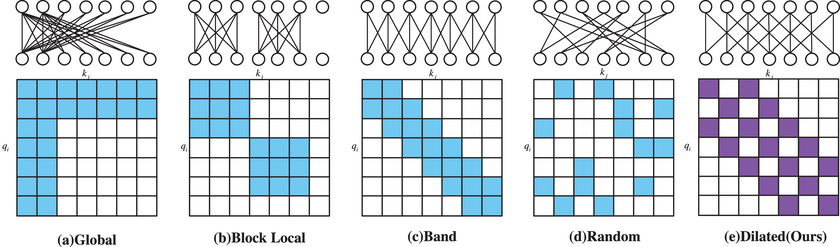
\includegraphics[width=1.0\textwidth]{sparse_attention_patterns.png}
    \captionof{figure}{So sánh các mẫu chú ý thưa (sparse attention). 
    (a) Chú ý toàn cục (Global). 
    (b) Chú ý theo khối cục bộ (Block Local). 
    (c) Chú ý theo dải (Band), hay còn gọi là cửa sổ trượt (Sliding Window). 
    (d) Chú ý ngẫu nhiên (Random). 
    (e) Chú ý giãn cách (Dilated). 
    Các mô hình như Longformer và BigBird thường kết hợp các mẫu này.}
    \label{fig:sparse_attention_patterns}
\end{center}

Hai mô hình tiên phong và tiêu biểu nhất cho trường phái này là Longformer và BigBird.

\subsubsection{Longformer: Kết hợp Cửa sổ trượt và Chú ý Toàn cục}
Longformer (Beltagy et al., 2020) \cite{beltagy2020longformer} đề xuất một mẫu chú ý kết hợp ba thành phần:

\paragraph{1. Chú ý Cửa sổ trượt (Sliding Window Attention)}
\begin{itemize}
    \item \textbf{Cơ chế:} Mỗi token chỉ chú ý đến một cửa sổ có kích thước cố định $w$ gồm các token xung quanh nó (ví dụ: $w/2$ token bên trái và $w/2$ token bên phải).
    \item \textbf{Mục đích:} Nắm bắt ngữ cảnh cục bộ, tương tự như trong các mô hình CNN. Đây là phần lớn các kết nối chú ý trong mô hình.
\end{itemize}

\paragraph{2. Chú ý Cửa sổ trượt Giãn cách (Dilated Sliding Window)}
\begin{itemize}
    \item \textbf{Cơ chế:} Để mở rộng "trường tiếp nhận" (receptive field) mà không tăng chi phí, Longformer sử dụng các cửa sổ trượt có "lỗ" (gaps) ở các lớp khác nhau. Ví dụ, ở một lớp, cửa sổ có thể chú ý đến các token cách nhau 1 vị trí, ở lớp khác, cách nhau 2 vị trí, v.v.
    \item \textbf{Mục đích:} Giúp thông tin từ các token xa hơn có thể được tích hợp vào biểu diễn của một token mà không cần kết nối trực tiếp.
\end{itemize}

\paragraph{3. Chú ý Toàn cục (Global Attention)}
\begin{itemize}
    \item \textbf{Cơ chế:} Một số ít các token được chọn trước được phép chú ý đến \textbf{tất cả} các token khác trong chuỗi, và ngược lại, tất cả các token khác cũng được phép chú ý đến chúng.
    \item \textbf{Mục đích:} Các token toàn cục này hoạt động như một "trung tâm thông tin", tổng hợp và phân phối thông tin trên toàn bộ chuỗi. Các token này thường được chọn một cách đặc biệt, ví dụ như token `[CLS]` trong các tác vụ phân loại.
\end{itemize}

Bằng cách kết hợp các mẫu này, Longformer giảm độ phức tạp tính toán xuống $O(n \cdot w)$, gần như tuyến tính với độ dài chuỗi $n$, cho phép nó xử lý các chuỗi lên tới 4096 token hoặc hơn.

\subsubsection{BigBird: Thêm các Mẫu Chú ý Ngẫu nhiên}
BigBird (Zaheer et al., 2020) \cite{zaheer2020big} có triết lý tương tự Longformer nhưng bổ sung thêm một thành phần:
\begin{itemize}
    \item Nó cũng sử dụng \textbf{Chú ý Cửa sổ trượt} và \textbf{Chú ý Toàn cục}.
    \item Điểm mới lạ là nó thêm vào \textbf{Chú ý Ngẫu nhiên (Random Attention)}. Mỗi token sẽ chú ý đến một số lượng nhỏ $r$ các token được chọn ngẫu nhiên từ toàn bộ chuỗi.
\end{itemize}
Các tác giả đã chứng minh về mặt lý thuyết rằng một mô hình kết hợp ba loại chú ý này (cửa sổ, toàn cục, ngẫu nhiên) có thể xấp xỉ được các thuộc tính của cơ chế chú ý đầy đủ và là một bộ xấp xỉ hàm phổ quát (universal function approximator).

\subsection{Các phương pháp khác: Thoát khỏi Self-Attention Bậc hai}
\label{ssec:other_long_context_methods}

Sparse Attention là một hướng tiếp cận, nhưng không phải là duy nhất. Một hướng đi khác, cấp tiến hơn, là đặt câu hỏi: "Liệu chúng ta có thực sự cần cơ chế chú ý bậc hai không?". Điều này đã dẫn đến sự ra đời của các kiến trúc hoàn toàn mới.
\subsubsection{Cải tiến Mã hóa Vị trí (Positional Encoding)}
Một hướng quan trọng khác để giúp Transformer xử lý ngữ cảnh dài là cải tiến cách nó hiểu về vị trí của token.
\paragraph{ALiBi (Attention with Linear Biases)}
Thay vì thêm mã hóa vị trí vào embedding, ALiBi \cite{press2021train} trực tiếp sửa đổi ma trận điểm chú ý.
\begin{itemize}
    \item \textbf{Cơ chế:} Trước khi qua softmax, điểm chú ý giữa token $i$ và $j$ sẽ bị trừ đi một "án phạt" (penalty) tỷ lệ thuận với khoảng cách của chúng: $\text{score}(i, j) - m \cdot |i - j|$. Trong đó, $m$ là một hệ số học được cho mỗi "đầu" chú ý.
    \item \textbf{Trực giác:} "Các từ càng xa nhau thì càng ít liên quan".
    \item \textbf{Lợi ích:} ALiBi cho thấy khả năng \textbf{ngoại suy (extrapolation)} ấn tượng. Một mô hình được huấn luyện trên ngữ cảnh 2048 token với ALiBi có thể hoạt động tốt trên ngữ cảnh 4096 token hoặc dài hơn mà không cần fine-tuning.
\end{itemize}

\paragraph{RoPE Scaling}
Các mô hình sử dụng Rotary Position Embedding (RoPE) như Llama thường gặp khó khăn khi ngoại suy ra các chuỗi dài hơn độ dài huấn luyện. Các kỹ thuật RoPE Scaling giải quyết vấn đề này.
\begin{itemize}
    \item \textbf{Vấn đề:} RoPE sử dụng các hàm sin/cos với tần số phụ thuộc vào vị trí. Khi vị trí vượt quá giới hạn huấn luyện, các tần số này bắt đầu lặp lại hoặc tạo ra các mẫu không ổn định.
    \item \textbf{Giải pháp (ví dụ:\cite{bloc972023ntkaware}, YaRN \cite{peng2023yarn}):} Các kỹ thuật này sửa đổi "bước sóng" (wavelength) của các hàm sin/cos, về cơ bản là "kéo dãn" không gian vị trí để có thể chứa các chuỗi dài hơn mà không phá vỡ các mối quan hệ tương đối đã học được ở cự ly gần.
\end{itemize}
\subsubsection{Mô hình Trạng thái (State Space Models - SSMs) và Mamba}
Đây là một trong những hướng nghiên cứu thú vị và hứa hẹn nhất gần đây.

\paragraph{Nguồn gốc từ Lý thuyết Điều khiển}
SSMs có nguồn gốc từ lý thuyết điều khiển và xử lý tín hiệu. Chúng được thiết kế để mô hình hóa các hệ thống động liên tục. Ý tưởng cốt lõi là duy trì một \textbf{trạng thái ẩn (state) $h(t)$ nhỏ, có kích thước cố định}, và cập nhật nó một cách liên tục theo thời gian dựa trên đầu vào $x(t)$.
$$ h'(t) = \mathbf{A}h(t) + \mathbf{B}x(t) $$
$$ y(t) = \mathbf{C}h(t) + \mathbf{D}x(t) $$
Trong đó $\mathbf{A, B, C, D}$ là các ma trận tham số.

\paragraph{Thách thức và Giải pháp}
Việc áp dụng trực tiếp SSMs vào học sâu là rất khó khăn về mặt tính toán. Các mô hình như S4 (Structured State Space for Sequence Modeling) \cite{gu2021efficiently} đã giải quyết vấn đề này bằng cách tìm ra một cách hiệu quả để "rời rạc hóa" (discretize) các công thức liên tục này, cho phép chúng được tính toán như một phép tích chập lớn trong quá trình huấn luyện (rất nhanh và song song) và như một RNN trong quá trình suy luận (hiệu quả về bộ nhớ).

\paragraph{Mamba: SSMs có Chọn lọc (Selective SSMs)}
Mamba (Gu \& Dao, 2023) \cite{gu2023mamba} là một bước đột phá lớn dựa trên SSMs. Nó nhận ra rằng một hạn chế của các SSMs trước đó là các ma trận $\mathbf{A, B, C, D}$ là \textbf{cố định}, không phụ thuộc vào đầu vào. Điều này có nghĩa là mô hình không thể thay đổi hành vi của mình dựa trên nội dung cụ thể mà nó đang xử lý.

Mamba đã giải quyết vấn đề này bằng cách làm cho các ma trận $\mathbf{B, C}$ và một tham số bước $\Delta$ \textbf{phụ thuộc vào đầu vào (input-dependent)}.
\paragraph{So sánh SSMs và RNNs truyền thống}
Ở chế độ suy luận, SSM hoạt động tuần tự giống như một RNN. Tuy nhiên, có một sự khác biệt cốt lõi:
\begin{itemize}
    \item \textbf{RNNs (LSTM/GRU):} Việc cập nhật trạng thái ẩn đi qua các cổng phi tuyến phức tạp (sigmoid, tanh). Các cổng này, mặc dù mạnh mẽ, lại làm cho gradient khó chảy ngược qua các chuỗi dài và khó song song hóa trong quá trình huấn luyện.
    \item \textbf{SSMs:} Việc cập nhật trạng thái về bản chất là \textbf{tuyến tính} ($h'(t) = \mathbf{A}h(t) + \dots$). Bản chất tuyến tính này, kết hợp với các ma trận được cấu trúc đặc biệt, cho phép gradient chảy ngược qua các chuỗi rất dài mà không bị triệt tiêu, đồng thời cho phép nó được biến đổi thành một phép tích chập song song hóa được khi huấn luyện.
\end{itemize}
Mamba kế thừa những ưu điểm này và thêm vào đó khả năng chọn lọc thông tin, tạo ra một kiến trúc vừa hiệu quả vừa mạnh mẽ.
\begin{tcolorbox}[
    title=Cơ chế Chọn lọc của Mamba,
    colback=green!5!white, colframe=green!60!black, fonttitle=\bfseries
]
Mamba có khả năng \textbf{chọn lọc} thông tin. Dựa trên token đầu vào hiện tại, nó có thể quyết định:
\begin{enumerate}
    \item \textbf{Tập trung:} Nếu một thông tin quan trọng xuất hiện, nó có thể "mở cổng" để cho thông tin đó đi vào trạng thái ẩn.
    \item \textbf{Lãng quên:} Nếu thông tin hiện tại không còn liên quan, nó có thể "nén" hoặc "quên" đi trạng thái ẩn cũ và đặt lại.
\end{enumerate}
Khả năng chọn lọc này cho phép Mamba nén ngữ cảnh một cách linh hoạt, chỉ giữ lại những gì cần thiết, một khả năng mà các mô hình tích chập hay RNN tuyến tính trước đó không có được.
\end{tcolorbox}

\paragraph{Ưu điểm của Mamba so với Transformer}
\begin{itemize}
    \item \textbf{Độ phức tạp tuyến tính:} Cả huấn luyện và suy luận đều có độ phức tạp $O(n)$, nhanh hơn nhiều so với $O(n^2)$ của Transformer.
    \item \textbf{Suy luận nhanh:} Tốc độ suy luận (sinh từ mới) nhanh hơn Transformer vì nó không cần tính toán lại ma trận chú ý khổng lồ ở mỗi bước.
\end{itemize}
Mamba và các kiến trúc dựa trên SSMs đang nổi lên như một đối thủ cạnh tranh thực sự với Transformer, đặc biệt là trong các kịch bản yêu cầu ngữ cảnh cực dài và hiệu quả tính toán cao.

\subsubsection{Các hướng tiếp cận khác}
Ngoài ra, còn có các hướng tiếp cận khác như:
\begin{itemize}
    \item \textbf{Tích chập có cửa sổ lớn (Large Kernel Convolutions):} Sử dụng các lớp tích chập 1D nhưng với kích thước kernel rất lớn để mô phỏng sự tương tác tầm xa.
    \item \textbf{Phương pháp đệ quy (Recurrence):} Cố gắng đưa trở lại một số dạng của cơ chế RNN để nén thông tin từ các đoạn (chunks) văn bản dài.
\end{itemize}

Việc xử lý ngữ cảnh dài vẫn là một trong những lĩnh vực nghiên cứu năng động nhất, hứa hẹn sẽ mở khóa nhiều khả năng mới cho các mô hình ngôn ngữ trong tương lai.
% % !TEX root = ../main.tex
% File: chapters_part1/chap4_5.tex
% Nội dung cho Chương 4, Phần 5

\section{Lý thuyết về Mixture-of-Experts (MoE)}
\label{sec:mixture_of_experts}

Khi chúng ta nói về việc "tăng quy mô" (scaling up) các mô hình ngôn ngữ, cách tiếp cận thông thường là làm cho các mô hình trở nên "dày đặc" hơn (denser) - tức là tăng số lớp, tăng số chiều ẩn, tăng số đầu chú ý. Tuy nhiên, cách tiếp cận này có một giới hạn: để xử lý mỗi token, \textbf{toàn bộ các tham số của mô hình đều phải được kích hoạt}. Điều này dẫn đến chi phí tính toán cực kỳ lớn ở cả quá trình huấn luyện và suy luận.

Mixture-of-Experts (MoE) \cite{shazeer2017outrageously, fedus2022switch} đưa ra một giải pháp thanh lịch cho vấn đề này, dựa trên một triết lý rất con người:

\begin{tcolorbox}[
    title=Triết lý của Mixture-of-Experts,
    colback=yellow!10!white, colframe=yellow!50!black, fonttitle=\bfseries
]
"Không cần phải huy động toàn bộ bộ não để giải quyết mọi vấn đề. Thay vào đó, hãy có một hội đồng gồm nhiều \textbf{chuyên gia (experts)}, mỗi người chuyên về một lĩnh vực khác nhau. Đối với mỗi vấn đề cụ thể, chỉ cần hỏi ý kiến của một vài chuyên gia phù hợp nhất."
\end{tcolorbox}

Trong bối cảnh của Transformer, MoE cho phép tăng số lượng tham số của mô hình lên rất lớn, nhưng lại giữ cho chi phí tính toán trên mỗi token không đổi hoặc chỉ tăng nhẹ. Đây được gọi là \textbf{tăng quy mô thưa thớt (sparse scaling)}.

\subsection{Kiến trúc và Nguyên lý hoạt động}
\label{ssec:moe_architecture}

Kiến trúc MoE không phải là một mô hình hoàn toàn mới. Thay vào đó, nó là một cách để sửa đổi các khối Transformer hiện có. Cụ thể, trong một khối Transformer tiêu chuẩn, lớp \textbf{Feed-Forward Network (FFN)} được thay thế bằng một \textbf{lớp MoE}.

Một lớp MoE bao gồm hai thành phần chính:
\begin{enumerate}
    \item \textbf{Một tập hợp gồm $N$ mạng FFN độc lập, gọi là các "chuyên gia" (Experts).} Ví dụ, $N$ có thể là 8, 16, hoặc 64. Mỗi chuyên gia này có bộ trọng số riêng.
    \item \textbf{Một mạng cổng (Gating Network) nhỏ.} Đây là một mạng nơ-ron có nhiệm vụ quyết định xem nên gửi mỗi token đến chuyên gia nào.
\end{enumerate}

\begin{center}
    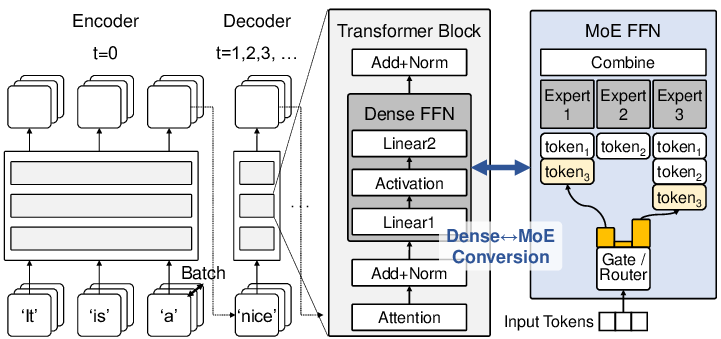
\includegraphics[width=1.0\textwidth]{moe_transformer_block.png}
    \captionof{figure}{So sánh một khối Transformer tiêu chuẩn (trái) và một khối Transformer với lớp MoE (phải). Lớp FFN dày đặc được thay thế bằng một mạng cổng và nhiều chuyên gia FFN thưa thớt.}
    \label{fig:moe_transformer_block}
\end{center}

\subsubsection{Dòng chảy dữ liệu của một token}
Khi một token (được biểu diễn bằng vector $x$) đi vào lớp MoE, quá trình sau sẽ xảy ra:

\paragraph{Bước 1: Định tuyến bởi Mạng cổng (Routing by the Gating Network)}
\begin{itemize}
    \item Token $x$ được đưa vào mạng cổng.
    \item Mạng cổng, thường là một lớp tuyến tính đơn giản, sẽ xuất ra một vector logits có số chiều bằng số chuyên gia ($N$).
    \item Một hàm `softmax` được áp dụng lên vector logits này để tạo ra một phân phối xác suất, $G(x) = (g_1, g_2, \dots, g_N)$, trong đó $g_i$ là "điểm số" hoặc "mức độ tin cậy" mà mạng cổng dành cho chuyên gia thứ $i$.
\end{itemize}

\paragraph{Bước 2: Chọn các Chuyên gia "Top-K"}
\begin{itemize}
    \item Thay vì gửi token đến tất cả các chuyên gia (điều này sẽ làm mất đi tính hiệu quả), hệ thống chỉ chọn ra $k$ chuyên gia có điểm số cao nhất (Top-K routing). Thông thường, $k$ là một số rất nhỏ, ví dụ $k=1$ hoặc $k=2$.
    \item Ví dụ, nếu $k=2$ và chuyên gia thứ 3 và thứ 5 có điểm số cao nhất, thì token này sẽ chỉ được gửi đến hai chuyên gia này. Tất cả các chuyên gia khác sẽ không được kích hoạt cho token này.
\end{itemize}

\paragraph{Bước 3: Xử lý bởi các Chuyên gia}
\begin{itemize}
    \item Token $x$ được đưa qua các mạng FFN của $k$ chuyên gia đã được chọn.
    \item Kết quả đầu ra là $k$ vector: $E_1(x), E_2(x), \dots, E_k(x)$.
\end{itemize}

\paragraph{Bước 4: Tổng hợp có trọng số}
\begin{itemize}
    \item Đầu ra cuối cùng của lớp MoE, $y$, là một tổng có trọng số của đầu ra từ các chuyên gia được chọn. Các trọng số này chính là các điểm số $g_i$ từ mạng cổng đã được chuẩn hóa.
    $$ y = \sum_{i \in \text{TopK}} g_i \cdot E_i(x) $$
\end{itemize}

\subsubsection{Ví dụ: Mixtral 8x7B}
Mô hình Mixtral 8x7B nổi tiếng của Mistral AI là một ví dụ điển hình của MoE.
\begin{itemize}
    \item \textbf{8x7B có nghĩa là gì?} Nó có 8 chuyên gia, mỗi chuyên gia có khoảng 7 tỷ tham số. Tổng số tham số của các lớp MoE là $8 \times 7B = 56B$. Tuy nhiên, đây là số tham số "thưa thớt".
    \item \textbf{Top-2 Routing:} Tại mỗi lớp MoE, mỗi token chỉ được định tuyến đến 2 trong số 8 chuyên gia.
    \item \textbf{Chi phí tính toán:} Do đó, mặc dù tổng số tham số rất lớn, chi phí tính toán để xử lý một token chỉ tương đương với một mô hình dày đặc khoảng $2 \times 7B = 14B$ tham số (cộng với một chi phí nhỏ cho mạng cổng và các lớp khác). Mixtral đạt được chất lượng của một mô hình rất lớn với tốc độ và chi phí của một mô hình nhỏ hơn nhiều.
\end{itemize}
\begin{tcolorbox}[
    title={Các "Chuyên gia" có thực sự chuyên môn hóa không?},
    colback=blue!5!white, colframe=blue!75!black, fonttitle=\bfseries
]
Phép ẩn dụ về "hội đồng chuyên gia" rất hữu ích, nhưng sự chuyên môn hóa của các expert FFN trong thực tế lại trừu tượng hơn nhiều.
\begin{itemize}
    \item \textbf{Không phải là chuyên môn về chủ đề:} Các nghiên cứu đã chỉ ra rằng các expert thường không chuyên môn hóa theo các chủ đề dễ hiểu như "thể thao", "khoa học" hay "lịch sử". Việc định tuyến một token đến expert nào phụ thuộc nhiều vào các đặc trưng trừu tượng của vector biểu diễn của nó.
    \item \textbf{Chuyên môn hóa theo cụm cú pháp/ngữ nghĩa:} Thay vào đó, sự chuyên môn hóa có thể xảy ra ở mức độ thấp hơn. Ví dụ, một số chuyên gia có thể giỏi hơn trong việc xử lý các token là dấu câu, một số khác chuyên về các động từ, một số khác lại tập trung vào các token ở các lớp Transformer cụ thể (ví dụ, các token ở lớp đầu so với lớp cuối).
    \item \textbf{Sự dư thừa có chủ đích:} Có bằng chứng cho thấy các chuyên gia không hoàn toàn độc lập. Thường có sự dư thừa (redundancy) giữa chúng. Điều này có thể là một đặc tính hữu ích, giúp mô hình trở nên mạnh mẽ hơn: nếu một chuyên gia đưa ra kết quả kém, các chuyên gia khác có thể bù đắp.
\end{itemize}
Vì vậy, hãy xem các "chuyên gia" như các \textbf{nhóm tham số (parameter groups)} có thể học được, thay vì các chuyên gia về một lĩnh vực kiến thức cụ thể. Mạng cổng học cách kết hợp các nhóm tham số này một cách tối ưu cho từng token.
\end{tcolorbox}
\subsection{Thách thức trong việc Huấn luyện MoE}
\label{ssec:moe_training_challenges}

Mặc dù rất mạnh mẽ, việc huấn luyện MoE không hề đơn giản và đòi hỏi phải giải quyết một số thách thức đặc thù.

\paragraph{1. Thách thức về sự sụp đổ của việc định tuyến (Routing Collapse)}
Đây là vấn đề lớn nhất của MoE. Nếu không được kiểm soát, mạng cổng sẽ nhanh chóng học được một chiến lược "lười biếng": luôn gửi phần lớn các token đến một hoặc một vài chuyên gia "yêu thích" mà nó cho là tốt nhất.
\begin{itemize}
    \item \textbf{Hậu quả:}
        \begin{enumerate}
            \item \textbf{Lãng phí tham số:} Các chuyên gia khác không nhận được token, do đó không được huấn luyện và trở thành "dead wood". Mô hình MoE khổng lồ sẽ sụp đổ (collapse) thành một mô hình nhỏ hơn nhiều.
            \item \textbf{Mất ổn định huấn luyện:} Gradient sẽ chảy không đều, gây khó khăn cho quá trình tối ưu hóa.
        \end{enumerate}
\end{itemize}

\paragraph{Giải pháp: Hàm Mất mát Cân bằng Tải (Load Balancing Loss)}
Để giải quyết vấn đề này, người ta thêm một \textbf{hàm mất mát phụ trợ (auxiliary loss)} vào hàm mất mát chính của mô hình. Hàm mất mát này được thiết kế để khuyến khích sự phân bổ token đồng đều và thường bao gồm hai thành phần:
\begin{itemize}
    \item \textbf{Một thành phần khuyến khích tầm quan trọng (importance) đồng đều:} Nó phạt nếu tổng các điểm số (logits) mà mạng cổng gán cho mỗi chuyên gia trên toàn bộ một batch là không đồng đều. Điều này đảm bảo mỗi chuyên gia được coi là "quan trọng" như nhau về mặt tổng thể.
    \item \textbf{Một thành phần khuyến khích số lượng token (load) đồng đều:} Nó phạt nếu số lượng token được gửi đến mỗi chuyên gia trong một batch là không đồng đều. Điều này đảm bảo mỗi chuyên gia có "công việc" để làm.
\end{itemize}
Việc cân bằng giữa hàm mất mát chính (ví dụ, cross-entropy) và hàm mất mát phụ trợ này là một trong những khía cạnh nghệ thuật nhất khi huấn luyện các mô hình MoE.

\paragraph{Giải pháp bổ sung: Noisy Top-K Gating}
Một kỹ thuật khác là thêm nhiễu ngẫu nhiên (Gaussian noise) vào logits của mạng cổng trong quá trình huấn luyện.
$$ \text{logits}_{\text{noisy}} = \text{logits}_{\text{original}} + \text{Noise} $$
Nhiễu này buộc mô hình phải "khám phá" (explore) các lựa chọn định tuyến khác nhau thay vì chỉ đi theo con đường quen thuộc, giúp cải thiện sự cân bằng tải một cách tự nhiên.

\paragraph{2. Thách thức về Triển khai và Cơ sở hạ tầng}
\begin{itemize}
    \item \textbf{Bộ nhớ:} Mặc dù chi phí tính toán trên mỗi token thấp, toàn bộ các tham số của tất cả các chuyên gia vẫn phải được tải vào bộ nhớ của GPU, đòi hỏi các hệ thống có bộ nhớ cực lớn.
    \item \textbf{Giao tiếp mạng:} Trong các hệ thống huấn luyện phân tán, các token từ một GPU có thể cần được gửi đến các chuyên gia nằm trên một GPU khác, đòi hỏi băng thông mạng rất cao.
\end{itemize}

\subsection{Tổng kết về MoE}
Mixture-of-Experts là một sự thay đổi mô hình trong cách chúng ta xây dựng các mô hình ngôn ngữ lớn. Nó cho phép chúng ta tách rời \textbf{tổng số tham số} khỏi \textbf{chi phí tính toán trên mỗi token}.

Bằng cách sử dụng các chuyên gia thưa thớt, MoE mở ra một con đường để xây dựng các mô hình có quy mô khổng lồ (hàng nghìn tỷ tham số), có khả năng lưu trữ một lượng kiến thức cực lớn, trong khi vẫn duy trì được tốc độ huấn luyện và suy luận ở mức có thể quản lý được. Đây là một trong những công nghệ nền tảng quan trọng nhất cho thế hệ LLM tiếp theo.

\bigskip
\hrule
\bigskip

\begin{center}
    \textbf{\Large KẾT THÚC CHƯƠNG 4}
\end{center}

\textit{Chương 4 đã là một chuyến đi sâu vào trái tim của NLP hiện đại. Chúng ta đã mổ xẻ kiến trúc Transformer, hiểu được sức mạnh của cơ chế Tự chú ý, và phân loại ba họ mô hình chính -- Encoder-Only, Decoder-Only, và Encoder-Decoder -- đã được sinh ra từ nó. Chúng ta cũng đã khám phá các kỹ thuật tiên tiến cho phép các mô hình này đạt đến quy mô khổng lồ và xử lý ngữ cảnh dài hơn. Về cơ bản, chúng ta đã tìm hiểu cách các "mô hình nền tảng" (foundation models) được xây dựng. Giờ đây, khi đã hiểu rõ cách các mô hình nền tảng khổng lồ này được xây dựng, câu hỏi tiếp theo là: Làm thế nào để chúng ta "thuần hóa" và "chuyên môn hóa" chúng cho các bài toán cụ thể? Chương tiếp theo sẽ tập trung vào các kỹ thuật tinh chỉnh và căn chỉnh, biến những gã khổng lồ đa năng này thành những chuyên gia sắc bén.}

% \chapter{CÁC KIẾN TRÚC MẠNG NƠ-RON KINH ĐIỂN}
\label{chap:deep_learning_architectures}

Chào mừng bạn đến với kỷ nguyên học sâu của NLP. Trong chương 2, chúng ta đã thấy các mô hình thống kê như N-gram có thể nắm bắt các phụ thuộc cục bộ, nhưng lại bất lực trước các mối quan hệ tầm xa. Cuộc cách mạng word embedding đã cho chúng ta các vector từ mang đầy ngữ nghĩa, nhưng làm thế nào để kết hợp chúng lại nhằm hiểu được ý nghĩa của cả một câu hay một đoạn văn?

Chương này sẽ giới thiệu các kiến trúc mạng nơ-ron nền tảng được thiết kế đặc biệt để xử lý dữ liệu dạng chuỗi như ngôn ngữ tự nhiên. Những kiến trúc này không chỉ đơn thuần "nhìn" vào các từ một cách riêng lẻ, mà còn có khả năng "ghi nhớ" và "lý luận" dựa trên thông tin đã xử lý trước đó, cho phép chúng nắm bắt được ngữ cảnh và các phụ thuộc phức tạp trong câu.
% % !TEX root = ../main.tex
% File: chapters_part1/chap5_1.tex
% Nội dung cho Chương 5, Phần 1

\section{Các Phương pháp Tinh chỉnh (Fine-tuning)}
\label{sec:finetuning_methods}

\subsection{Học Chuyển giao (Transfer Learning): Nền tảng Tư duy}
\label{ssec:transfer_learning}
Trước khi đi vào kỹ thuật cụ thể, chúng ta cần hiểu triết lý nền tảng đằng sau nó: \textbf{Học Chuyển giao (Transfer Learning)}.

\begin{definition}{Học Chuyển giao}{def:transfer_learning}
    Học Chuyển giao là một phương pháp học máy trong đó một mô hình được phát triển cho một tác vụ A được tái sử dụng làm điểm khởi đầu cho một mô hình trong tác vụ B.
\end{definition}

Trong NLP, Học Chuyển giao đã trở thành một mô hình (paradigm) thống trị:
\begin{enumerate}
    \item \textbf{Giai đoạn Huấn luyện trước (Pre-training):} Huấn luyện một mô hình lớn (như BERT, GPT) trên một tác vụ chung (ví dụ: Masked Language Modeling, Next Token Prediction) với một kho dữ liệu khổng lồ, không cần gán nhãn. Giai đoạn này giúp mô hình học được các "biểu diễn" ngôn ngữ tổng quát. Đây là phần tốn kém nhất.
    \item \textbf{Giai đoạn Tinh chỉnh (Fine-tuning):} Lấy mô hình đã được huấn luyện trước và tiếp tục huấn luyện nó trên một bộ dữ liệu nhỏ hơn, đã được gán nhãn, dành riêng cho tác vụ mục tiêu (ví dụ: phân loại cảm xúc).
\end{enumerate}

\begin{center}
    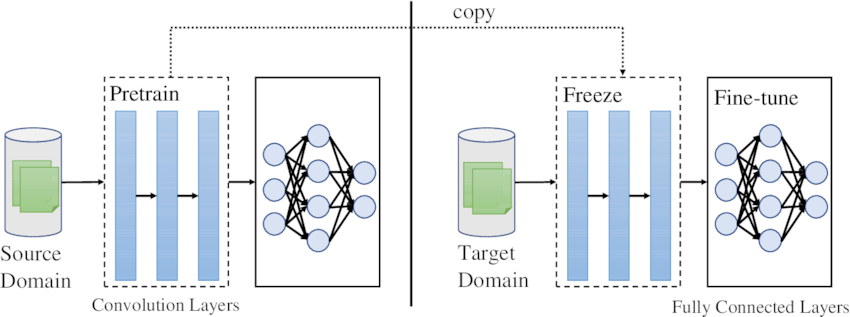
\includegraphics[width=0.8\textwidth]{transfer_learning_paradigm.png}
    \captionof{figure}{Mô hình Học Chuyển giao trong NLP: Một mô hình được huấn luyện trước trên dữ liệu lớn, sau đó được tinh chỉnh trên một tác vụ cụ thể.}
    \label{fig:transfer_learning_paradigm}
\end{center}

\textbf{Tại sao Học Chuyển giao lại hiệu quả?}
\begin{itemize}
    \item \textbf{Tiết kiệm tài nguyên:} Chúng ta không cần phải huấn luyện một mô hình khổng lồ từ đầu cho mỗi tác vụ. Chúng ta tận dụng lại kiến thức đã được học từ quá trình pre-training tốn kém.
    \item \textbf{Cải thiện hiệu năng:} Các biểu diễn ngôn ngữ tổng quát học được từ dữ liệu lớn cung cấp một điểm khởi đầu tốt hơn nhiều so với việc khởi tạo trọng số ngẫu nhiên, giúp mô hình hội tụ nhanh hơn và đạt độ chính xác cao hơn, đặc biệt khi dữ liệu cho tác vụ cụ thể là có hạn.
    \item \textbf{Dân chủ hóa AI:} Cho phép các nhà phát triển và nhà nghiên cứu không có tài nguyên tính toán khổng lồ vẫn có thể xây dựng các ứng dụng NLP state-of-the-art bằng cách tinh chỉnh các mô hình đã được huấn luyện trước.
\end{itemize}

\subsection{Tinh chỉnh Toàn bộ (Full Fine-tuning)}
\label{ssec:full_finetuning}

Đây là phương pháp tinh chỉnh kinh điển và trực quan nhất.

\subsubsection{Cơ chế hoạt động}
\begin{itemize}
    \item \textbf{Bước 1: Tải mô hình đã huấn luyện trước.} Tải toàn bộ kiến trúc và trọng số của một mô hình như BERT hoặc RoBERTa.
    \item \textbf{Bước 2: Thay thế "đầu" của mô hình.} Mô hình gốc thường có một "đầu" (head) được thiết kế cho tác vụ pre-training (ví dụ, đầu MLM). Chúng ta sẽ loại bỏ cái đầu này và thay thế nó bằng một "đầu" mới, phù hợp với tác vụ hạ nguồn của mình.
        \begin{itemize}
            \item \textbf{Ví dụ (Phân loại câu):} Thêm một lớp tuyến tính (linear layer) đơn giản với một lớp softmax lên trên vector biểu diễn của token `[CLS]`. Số nơ-ron đầu ra của lớp này bằng số lớp cần phân loại.
            \item \textbf{Ví dụ (Gán nhãn chuỗi - NER):} Thêm một lớp tuyến tính lên trên vector biểu diễn của \textit{mỗi} token trong chuỗi.
        \end{itemize}
    \item \textbf{Bước 3: Huấn luyện trên dữ liệu của tác vụ mới.} Toàn bộ mô hình (cả phần thân đã được huấn luyện trước và cái đầu mới) được huấn luyện tiếp trên bộ dữ liệu gán nhãn của tác vụ mục tiêu.
    \item \textbf{Cập nhật trọng số:} Trong quá trình này, \textbf{tất cả các trọng số của mô hình}, từ lớp embedding dưới cùng đến lớp phân loại trên cùng, đều được cập nhật thông qua thuật toán lan truyền ngược để tối thiểu hóa hàm mất mát trên tác vụ mới.
\end{itemize}
Điều quan trọng là việc huấn luyện ở giai đoạn này thường sử dụng một \textbf{tốc độ học (learning rate) rất nhỏ}. Lý do là vì các trọng số đã được huấn luyện trước đã ở một điểm "khá tốt". Chúng ta chỉ muốn "tinh chỉnh" chúng một chút để thích ứng với dữ liệu mới, chứ không muốn phá vỡ các kiến thức quý giá đã học được bằng các bước cập nhật quá lớn.

\subsubsection{Chiến lược Tinh chỉnh Nâng cao}
Trong thực tế, việc tinh chỉnh không chỉ đơn giản là chạy lại quá trình huấn luyện. Có một số chiến lược để cải thiện hiệu quả:
\paragraph{Huấn luyện theo lớp phân biệt (Discriminative Layer-wise Training)}
\begin{itemize}
    \item \textbf{Trực giác:} Các lớp khác nhau của một mô hình học sâu học các loại đặc trưng khác nhau. Các lớp dưới cùng (gần input) học các đặc trưng rất chung (như cú pháp cơ bản), trong khi các lớp trên cùng học các đặc trưng trừu tượng và chuyên biệt hơn.
    \item \textbf{Chiến lược:} Khi tinh chỉnh, chúng ta nên cập nhật các lớp trên cùng nhiều hơn và các lớp dưới cùng ít hơn. Điều này được thực hiện bằng cách áp dụng các \textbf{tốc độ học khác nhau cho các lớp khác nhau}. Ví dụ, lớp phân loại mới có thể có learning rate là $10^{-3}$, các lớp Transformer trên cùng là $10^{-4}$, và các lớp Transformer dưới cùng là $10^{-5}$.
\end{itemize}

\paragraph{Rã đông Dần dần (Gradual Unfreezing)}
\begin{itemize}
    \item \textbf{Trực giác:} Để tránh "quên thảm khốc" (catastrophic forgetting) - nơi mô hình nhanh chóng quên đi kiến thức đã học trong quá trình pre-training - chúng ta nên giới thiệu dữ liệu mới một cách từ từ.
    \item \textbf{Chiến lược:}
        \begin{enumerate}
            \item Ban đầu, "đóng băng" (freeze) toàn bộ các lớp đã được huấn luyện trước và chỉ huấn luyện cái đầu phân loại mới trong một vài epoch.
            \item Sau đó, "rã đông" (unfreeze) lớp Transformer trên cùng và huấn luyện cả nó và cái đầu mới.
            \item Tiếp tục quá trình này, rã đông dần dần từng lớp từ trên xuống dưới, cho đến khi toàn bộ mô hình được huấn luyện.
        \end{enumerate}
\end{itemize}

\subsubsection{Ưu và Nhược điểm của Tinh chỉnh Toàn bộ}
\begin{tcolorbox}[
    title=Đánh giá Tinh chỉnh Toàn bộ (Full Fine-tuning),
    colback=blue!5!white, colframe=blue!75!black, fonttitle=\bfseries
]
\textbf{Ưu điểm:}
\begin{itemize}
    \item \textbf{Hiệu năng cao nhất:} Thường mang lại độ chính xác tốt nhất vì toàn bộ mô hình được tối ưu hóa một cách trọn vẹn cho tác vụ mục tiêu.
    \item \textbf{Tương đối đơn giản:} Là một phương pháp đã được thiết lập rõ ràng và dễ triển khai.
\end{itemize}
\textbf{Nhược điểm:}
\begin{itemize}
    \item \textbf{Cực kỳ tốn kém về tài nguyên:} Thách thức lớn nhất trong kỷ nguyên LLM. Nếu bạn có 10 tác vụ khác nhau, bạn phải lưu trữ \textbf{10 bản sao đầy đủ} của mô hình khổng lồ đã được tinh chỉnh, mỗi bản sao có thể nặng hàng trăm gigabyte.
    \item \textbf{Dễ bị "quên thảm khốc":} Nếu dữ liệu tinh chỉnh quá khác biệt so với dữ liệu pre-training, mô hình có thể mất đi các khả năng tổng quát của nó.
    \item \textbf{Rủi ro về bảo mật và ổn định:} Việc cập nhật toàn bộ trọng số có thể gây ra các hành vi không mong muốn.
\end{itemize}
\end{tcolorbox}

Những nhược điểm này, đặc biệt là về chi phí lưu trữ và tính toán, đã trở nên cực kỳ rõ rệt với sự bùng nổ của các mô hình hàng tỷ tham số. Điều này đã thúc đẩy mạnh mẽ sự phát triển của một hướng tiếp cận mới, hiệu quả hơn nhiều: \textbf{Kỹ thuật Tinh chỉnh Hiệu quả Tham số (Parameter-Efficient Fine-Tuning - PEFT)}, mà chúng ta sẽ khám phá chi tiết trong mục tiếp theo.
% % !TEX root = ../main.tex
% File: chapters_part1/chap5_2.tex
% Nội dung cho Chương 5, Phần 2

\section{Kỹ thuật Tinh chỉnh Hiệu quả Tham số (PEFT)}
\label{sec:peft}

Như đã phân tích ở mục trước, Tinh chỉnh Toàn bộ (Full Fine-tuning) trở nên cực kỳ tốn kém và không thực tế khi làm việc với các Mô hình Ngôn ngữ Lớn (LLMs) có hàng tỷ tham số. Việc lưu trữ và triển khai hàng chục bản sao đầy đủ của một mô hình 175 tỷ tham số cho các tác vụ khác nhau là một cơn ác mộng về mặt tài chính và kỹ thuật.

\textbf{Kỹ thuật Tinh chỉnh Hiệu quả Tham số (Parameter-Efficient Fine-Tuning - PEFT)} ra đời như một giải pháp cho vấn đề này.

\begin{tcolorbox}[
    title=Triết lý của PEFT,
    colback=green!5!white, colframe=green!60!black, fonttitle=\bfseries
]
Thay vì cập nhật \textbf{tất cả} các trọng số của mô hình lớn, chúng ta hãy \textbf{đóng băng (freeze)} toàn bộ mô hình gốc và chỉ huấn luyện một số lượng rất nhỏ các tham số \textbf{bổ sung (additional)} hoặc một \textbf{tập con} các tham số hiện có.
\end{tcolorbox}

Mục tiêu là đạt được hiệu năng gần bằng hoặc thậm chí tốt hơn Full Fine-tuning, trong khi chỉ cần huấn luyện và lưu trữ một phần rất nhỏ (thường < 1\%) của tổng số tham số. Điều này làm cho việc thích ứng LLM trở nên khả thi và hiệu quả hơn rất nhiều.

Có nhiều họ phương pháp PEFT khác nhau, chúng ta sẽ khám phá những phương pháp tiêu biểu và có ảnh hưởng nhất.

\subsection{LoRA: Thích ứng Thứ hạng Thấp (Low-Rank Adaptation)}
\label{ssec:lora}
LoRA (Hu et al., 2021) \cite{hu2021lora} là một trong những kỹ thuật PEFT phổ biến và thành công nhất hiện nay. Nó dựa trên một quan sát sâu sắc về cách các mạng nơ-ron học.

\subsubsection{Trực giác và Nền tảng Lý thuyết}
\begin{itemize}
    \item \textbf{Quan sát:} Các nhà nghiên cứu phát hiện ra rằng mặc dù các mô hình ngôn ngữ lớn có số chiều rất cao, nhưng sự thay đổi của các trọng số trong quá trình tinh chỉnh (tức là ma trận $\Delta W = W_{\text{fine-tuned}} - W_{\text{pre-trained}}$) thường có một "thứ hạng nội tại" (intrinsic rank) rất thấp.
    \item \textbf{Ý nghĩa:} Điều này có nghĩa là ma trận thay đổi trọng số $\Delta W$ (kích thước $d \times d$) có thể được xấp xỉ rất tốt bằng tích của hai ma trận nhỏ hơn nhiều, $A$ (kích thước $d \times r$) và $B$ (kích thước $r \times d$), trong đó $r$ (thứ hạng) là một số rất nhỏ so với $d$ (ví dụ: $r=8, d=4096$).
    \item \textbf{Kết luận:} Thay vì học ma trận $\Delta W$ khổng lồ với $d^2$ tham số, chúng ta có thể chỉ cần học hai ma trận nhỏ $A$ và $B$ với tổng số tham số chỉ là $2 \times d \times r$. Đây là một sự tiết kiệm rất lớn.
\end{itemize}

\subsubsection{Cơ chế hoạt động của LoRA}
LoRA áp dụng ý tưởng này vào các lớp cần nhiều tham số nhất trong Transformer, thường là các ma trận trọng số của các lớp tuyến tính trong cơ chế Self-Attention ($W_Q, W_K, W_V, W_O$).
\begin{enumerate}
    \item \textbf{Đóng băng mô hình gốc:} Toàn bộ trọng số của mô hình đã huấn luyện trước, $W_0$, được giữ nguyên và không cập nhật trong quá trình huấn luyện.
    \item \textbf{Thêm các ma trận phân rã:} Với mỗi ma trận trọng số $W_0$ mà chúng ta muốn thích ứng (ví dụ, $W_Q$), LoRA thêm vào hai ma trận "adapter" nhỏ là $A$ (khởi tạo ngẫu nhiên) và $B$ (khởi tạo bằng 0).
    \item \textbf{Sửa đổi quá trình truyền thẳng (Forward Pass):} Đầu ra của lớp được sửa đổi như sau:
        $$ h = W_0 x + \Delta W x = W_0 x + BAx $$
        Vector đầu vào $x$ sẽ đi qua hai nhánh song song:
        \begin{itemize}
            \item Nhánh chính đi qua ma trận $W_0$ đã đóng băng.
            \item Nhánh LoRA đi qua ma trận $A$ trước (giảm chiều từ $d$ xuống $r$), sau đó qua ma trận $B$ (tăng chiều từ $r$ trở lại $d$).
        \end{itemize}
        Kết quả của hai nhánh này sau đó được cộng lại với nhau.
    \item \textbf{Huấn luyện:} Chỉ có các ma trận $A$ và $B$ được huấn luyện. Tất cả các tham số khác đều bị đóng băng.
\end{enumerate}

\begin{center}
    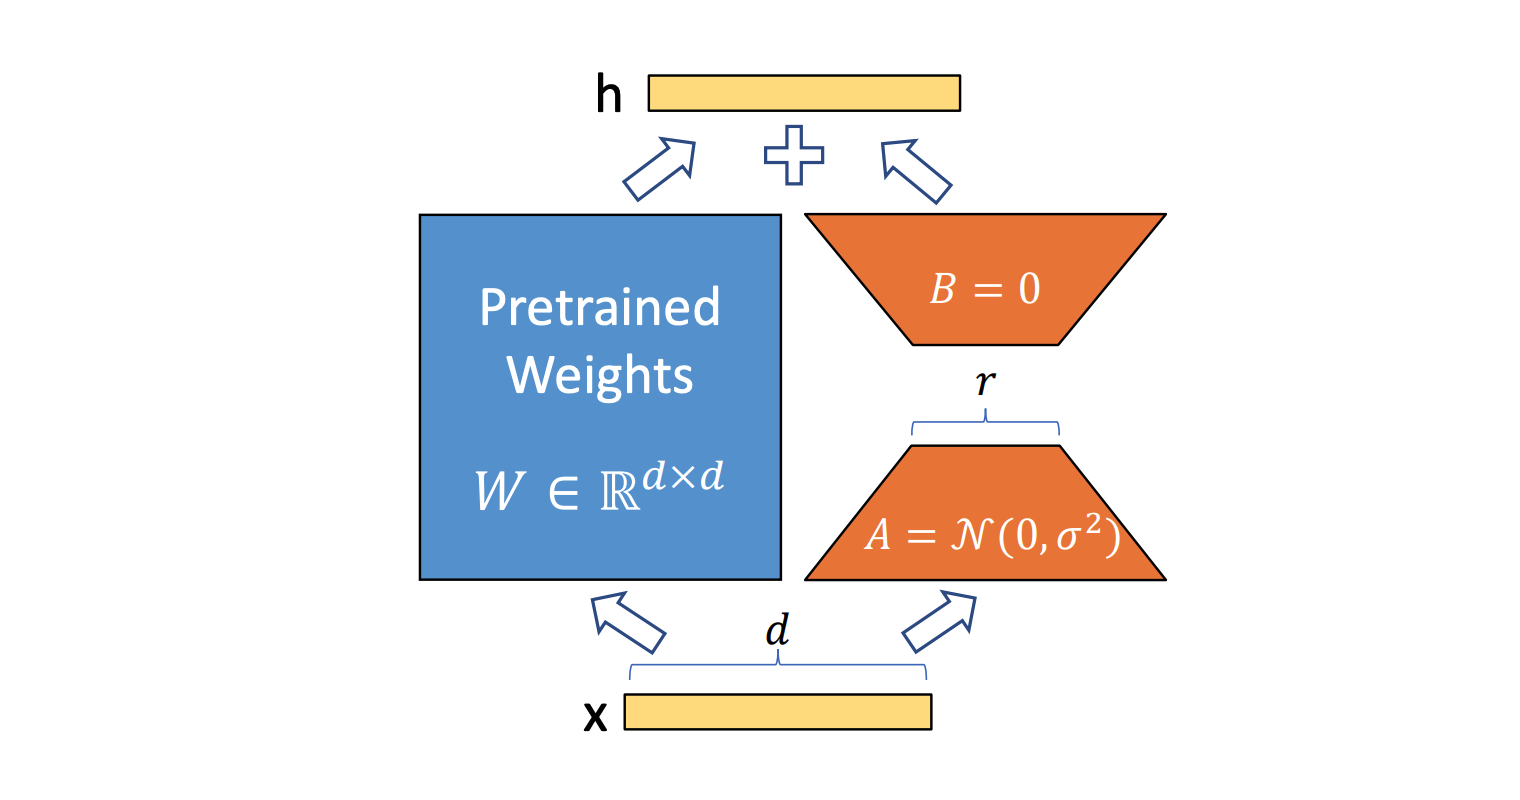
\includegraphics[width=1.0\textwidth]{lora_mechanism.png}
    \captionof{figure}{Cơ chế hoạt động của LoRA. Trọng số gốc $W_0$ được đóng băng. Một nhánh phụ song song được thêm vào, bao gồm hai ma trận thứ hạng thấp $A$ và $B$. Chỉ có $A$ và $B$ được cập nhật trong quá trình huấn luyện.}
    \label{fig:lora_mechanism}
\end{center}

\subsubsection{Lợi ích của LoRA}
\begin{itemize}
    \item \textbf{Hiệu quả về lưu trữ:} Thay vì lưu một bản sao 13 tỷ tham số cho mỗi tác vụ, bạn chỉ cần lưu các ma trận LoRA A và B, có thể chỉ vài megabyte.
    \item \textbf{Chuyển đổi tác vụ nhanh chóng:} Có thể "cắm" và "rút" các adapter LoRA khác nhau vào cùng một mô hình nền tảng để chuyển đổi giữa các tác vụ mà không cần tốn thời gian tải lại toàn bộ mô hình.
    \item \textbf{Không có độ trễ suy luận (Inference Latency):} Sau khi huấn luyện xong, các trọng số LoRA ($BA$) có thể được \textbf{gộp (merged)} vào trọng số gốc ($W = W_0 + BA$). Quá trình suy luận sau đó diễn ra trên một ma trận duy nhất $W$, không có thêm bất kỳ chi phí tính toán nào so với mô hình gốc.
\end{itemize}

\subsection{QLoRA: Lượng tử hóa LoRA (Quantized LoRA)}
\label{ssec:qlora}
QLoRA (Dettmers et al., 2023) \cite{dettmers2023qlora} là một cải tiến đột phá của LoRA, giúp giảm yêu cầu về bộ nhớ GPU xuống mức cực thấp, cho phép tinh chỉnh các mô hình hàng tỷ tham số trên các GPU dành cho người tiêu dùng.

\subsubsection{Ý tưởng cốt lõi}
QLoRA kết hợp LoRA với một kỹ thuật gọi là \textbf{lượng tử hóa (quantization)}.
\begin{itemize}
    \item \textbf{Vấn đề:} Mặc dù LoRA chỉ huấn luyện một số ít tham số, nó vẫn yêu cầu phải \textbf{tải toàn bộ mô hình gốc vào bộ nhớ GPU} để thực hiện quá trình truyền thẳng (forward pass). Với các mô hình lớn, các trọng số này (thường ở định dạng 16-bit) vẫn chiếm một lượng VRAM khổng lồ.
    \item \textbf{Giải pháp của QLoRA:} Tải mô hình nền tảng đã được \textbf{lượng tử hóa xuống định dạng 4-bit}. Tức là, mỗi trọng số chỉ dùng 4 bit để lưu trữ thay vì 16 bit, giảm yêu cầu bộ nhớ đi 4 lần.
    \item \textbf{Thách thức:} Việc huấn luyện trực tiếp trên các trọng số 4-bit là không ổn định.
    \item \textbf{Sự đột phá của QLoRA:} Nó giới thiệu một kiểu dữ liệu 4-bit mới gọi là \textbf{4-bit NormalFloat (NF4)} và kỹ thuật \textbf{Double Quantization} để giảm thiểu mất mát thông tin. Quan trọng nhất, trong quá trình truyền thẳng, các trọng số 4-bit của mô hình nền tảng được \textbf{giải lượng tử hóa (de-quantized) về định dạng 16-bit "ngay khi cần"} cho việc tính toán, sau đó bị loại bỏ khỏi bộ nhớ. Gradient vẫn được lan truyền ngược qua các adapter LoRA ở định dạng 16-bit.
\end{itemize}

Nhờ QLoRA, việc tinh chỉnh một mô hình 65 tỷ tham số có thể được thực hiện trên một GPU duy nhất với 48GB VRAM, một điều không tưởng trước đây.

\subsection{Adapter-tuning}
\label{ssec:adapter_tuning}
Đây là một trong những họ phương pháp PEFT \cite{houlsby2019parameter} đầu tiên, có trước cả LoRA.
\begin{itemize}
    \item \textbf{Kiến trúc:} Thay vì thêm các nhánh song song, Adapter-tuning chèn các module nhỏ, gọi là \textbf{các lớp adapter (adapter layers)}, vào \textbf{bên trong} mỗi khối Transformer, thường là sau lớp Multi-Head Attention và lớp FFN.
    \item \textbf{Cơ chế:} Các lớp adapter này thường có kiến trúc "cổ chai" (bottleneck): một lớp tuyến tính giảm chiều, một hàm kích hoạt phi tuyến, và một lớp tuyến tính tăng chiều trở lại.
    \item \textbf{Huấn luyện:} Tương tự, toàn bộ mô hình gốc được đóng băng và chỉ có các tham số của các lớp adapter này được huấn luyện.
    \item \textbf{So với LoRA:} Adapter có nhược điểm là chúng thêm vào độ trễ suy luận vì đầu ra phải đi qua các lớp bổ sung một cách tuần tự. LoRA khắc phục được điều này nhờ khả năng gộp trọng số.
\end{itemize}

\subsection{Prompt-based Tuning: Điều chỉnh trên Lớp Đầu vào}
\label{ssec:prompt_tuning}
Các phương pháp trên can thiệp vào trọng số của mô hình. Một hướng tiếp cận khác, cấp tiến hơn, là: \textbf{giữ nguyên hoàn toàn mô hình và chỉ điều chỉnh đầu vào}.

\subsubsection{Prompt-Tuning}
\begin{itemize}
    \item \textbf{Ý tưởng:} Thay vì tinh chỉnh các trọng số khổng lồ, hãy học cách tìm ra "prompt" tốt nhất cho mô hình. Nhưng thay vì tìm kiếm các từ trong ngôn ngữ tự nhiên (hard prompt), Prompt-Tuning \cite{lester2021power} học một chuỗi các \textbf{vector embedding "mềm" (soft prompts)} liên tục.
    \item \textbf{Cơ chế:} Một số lượng nhỏ ($k$) các vector prompt có thể huấn luyện được sẽ được \textbf{chèn vào phía trước} chuỗi embedding đầu vào. Toàn bộ mô hình gốc được đóng băng. Trong quá trình huấn luyện, chỉ có các vector prompt này được cập nhật thông qua lan truyền ngược.
    \item \textbf{Lợi ích:} Cực kỳ hiệu quả về tham số (chỉ cần học vài nghìn tham số) và dễ dàng lưu trữ, chia sẻ các "prompt" đã được học cho các tác vụ khác nhau.
\end{itemize}

\subsubsection{Prefix-Tuning}
\begin{itemize}
    \item \textbf{Ý tưởng:} Tương tự Prompt-Tuning, nhưng thay vì chỉ chèn các vector vào lớp embedding đầu vào, Prefix-Tuning \cite{li2021prefix} chèn các tiền tố (prefixes) có thể huấn luyện được vào \textbf{mỗi lớp Transformer} của mô hình.
    \item \textbf{Cơ chế:} Các tiền tố này hoạt động như một "ngữ cảnh ảo" dành riêng cho tác vụ, giúp điều khiển hành vi của mỗi lớp một cách trực tiếp hơn.
    \item \textbf{Hiệu năng:} Thường cho kết quả tốt hơn Prompt-Tuning nhưng có nhiều tham số hơn để huấn luyện.
\end{itemize}

Các kỹ thuật PEFT đã thay đổi hoàn toàn cách chúng ta làm việc với LLMs, giúp việc tùy chỉnh các mô hình khổng lồ trở nên khả thi, tiết kiệm và linh hoạt hơn bao giờ hết.
% % !TEX root = ../main.tex
% File: chapters_part1/chap5_3.tex
% Nội dung cho Chương 5, Phần 3

\section{Kỹ thuật Prompt Engineering và Học trong Ngữ cảnh (In-context Learning)}
\label{sec:prompt_engineering_icl}

Với sự ra đời của các Mô hình Ngôn ngữ Lớn (LLMs) có quy mô hàng trăm tỷ tham số (ví dụ như họ GPT), một khả năng đáng kinh ngạc đã xuất hiện, được gọi là \textbf{Học trong Ngữ cảnh (In-context Learning - ICL)}.

\begin{definition}{Học trong Ngữ cảnh (ICL)}{def:in_context_learning}
    Học trong Ngữ cảnh là khả năng của một LLM có thể học và thực hiện một tác vụ mới chỉ bằng cách được cung cấp một vài ví dụ minh họa ngay trong \textbf{câu lệnh đầu vào (prompt)}, mà \textbf{không cần bất kỳ sự cập nhật trọng số nào} của mô hình.
\end{definition}

Nói cách khác, mô hình "học" bằng cách suy luận từ các ví dụ được đưa ra trong "bộ nhớ ngắn hạn" (ngữ cảnh của prompt), thay vì "học" bằng cách cập nhật "bộ nhớ dài hạn" (trọng số của mô hình) thông qua quá trình fine-tuning.

Khả năng này đã khai sinh ra một lĩnh vực hoàn toàn mới: \textbf{Kỹ thuật Thiết kế Câu lệnh (Prompt Engineering)} -- nghệ thuật và khoa học của việc thiết kế các prompt hiệu quả để khai thác tối đa tiềm năng của LLMs.

\subsection{Các cấp độ của Học trong Ngữ cảnh: Zero-shot, One-shot, Few-shot}
\label{ssec:shot_learning}

Khả năng ICL của LLMs thường được phân loại dựa trên số lượng ví dụ (`n`) được cung cấp trong prompt.

\subsubsection{Zero-shot Learning (Học không cần ví dụ, n=0)}
\begin{itemize}
    \item \textbf{Cơ chế:} Chỉ cung cấp cho mô hình một mô tả về tác vụ và câu hỏi cần trả lời, không kèm theo bất kỳ ví dụ minh họa nào.
    \item \textbf{Trực giác:} Đây là bài kiểm tra cuối cùng về khả năng tổng quát hóa của mô hình. Nó phải dựa hoàn toàn vào kiến thức đã học được trong quá trình pre-training để hiểu và thực hiện yêu cầu.
    \item \textbf{Ví dụ (Phân tích cảm xúc):}
        \begin{tcolorbox}[colback=gray!5!white, colframe=gray!50!black]
        \textbf{Prompt:} \\
        Phân loại cảm xúc của câu sau đây là Tích cực, Tiêu cực, hoặc Trung tính. \\
        Câu: Món ăn này thật tuyệt vời! \\
        Cảm xúc: 
        \end{tcolorbox}
        \textbf{Đầu ra mong muốn:} `Tích cực`
\end{itemize}

\subsubsection{One-shot Learning (Học với một ví dụ, n=1)}
\begin{itemize}
    \item \textbf{Cơ chế:} Cung cấp cho mô hình \textbf{một ví dụ} duy nhất về cặp (đầu vào, đầu ra) để làm mẫu, trước khi đưa ra câu hỏi thực sự.
    \item \textbf{Trực giác:} Một ví dụ duy nhất giúp mô hình "định vị" được tác vụ, hiểu rõ hơn về định dạng đầu ra mong muốn và bối cảnh cụ thể.
    \item \textbf{Ví dụ (Dịch từ vô nghĩa):}
        \begin{tcolorbox}[colback=gray!5!white, colframe=gray!50!black]
        \textbf{Prompt:} \\
        Dịch từ "glorp" sang tiếng Việt có nghĩa là "vui vẻ". \\
        Dịch từ "flumph" sang tiếng Việt có nghĩa là gì?
        \end{tcolorbox}
        \textbf{Đầu ra mong muốn:} Một từ vô nghĩa khác, thể hiện mô hình đã hiểu "quy luật" của tác vụ.
\end{itemize}

\subsubsection{Few-shot Learning (Học với vài ví dụ, n > 1)}
\begin{itemize}
    \item \textbf{Cơ chế:} Cung cấp cho mô hình \textbf{một vài ví dụ} (thường từ 2 đến vài chục) để minh họa cho tác vụ.
    \item \textbf{Trực giác:} Càng nhiều ví dụ, mô hình càng có nhiều thông tin để suy luận ra quy luật và mẫu hình của tác vụ, từ đó đưa ra câu trả lời chính xác hơn. Đây là phương pháp phổ biến và hiệu quả nhất trong ICL.
    \item \textbf{Ví dụ (Phép cộng):}
        \begin{tcolorbox}[colback=gray!5!white, colframe=gray!50!black]
        \textbf{Prompt:} \\
        Q: 2 + 2 = ? \\
        A: 4 \\
        \\
        Q: 5 + 8 = ? \\
        A: 13 \\
        \\
        Q: 12 + 3 = ? \\
        A: 
        \end{tcolorbox}
        \textbf{Đầu ra mong muốn:} `15`
\end{itemize}
Hiệu năng của mô hình thường tăng lên cùng với số lượng ví dụ, nhưng sẽ đạt đến một điểm bão hòa và bị giới hạn bởi độ dài ngữ cảnh của mô hình.

\subsection{Chuỗi Suy luận (Chain-of-Thought - CoT) Prompting}
\label{ssec:chain_of_thought}

\subsubsection{Vấn đề của Prompting Tiêu chuẩn}
Với các bài toán đòi hỏi suy luận nhiều bước (ví dụ: các bài toán logic, toán học), phương pháp few-shot tiêu chuẩn thường thất bại. Mô hình có thể cố gắng "đoán" câu trả lời cuối cùng một cách trực tiếp và thường đưa ra kết quả sai.

\subsubsection{Giải pháp của CoT: ''Hãy suy nghĩ từng bước''}
Chain-of-Thought (CoT) Prompting (Wei et al., 2022) Prompting \cite{wei2022chain} là một kỹ thuật đơn giản nhưng cực kỳ mạnh mẽ.
\begin{tcolorbox}[
    title=Trực giác của Chain-of-Thought,
    colback=yellow!10!white, colframe=yellow!50!black, fonttitle=\bfseries
]
Thay vì chỉ cung cấp các ví dụ (Câu hỏi, Trả lời), chúng ta hãy cung cấp các ví dụ bao gồm cả \textbf{quá trình suy luận từng bước (step-by-step reasoning)} dẫn đến câu trả lời cuối cùng. Điều này khuyến khích mô hình "bắt chước" quá trình suy nghĩ đó, phân rã một bài toán phức tạp thành các bước trung gian đơn giản hơn.
\end{tcolorbox}

\begin{example}{So sánh Standard Prompting và CoT Prompting}{ex:cot_comparison}
    \textbf{Bài toán:} Roger có 5 quả bóng tennis. Anh ấy mua thêm 2 hộp, mỗi hộp có 3 quả. Hỏi bây giờ anh ấy có tất cả bao nhiêu quả bóng?
    
    \textbf{1. Standard Few-shot Prompting (Thường thất bại):}
    \begin{tcolorbox}[colback=red!5!white, colframe=red!60!black]
    Q: Một người bán hoa quả có 23 quả táo. Nếu anh ta dùng 20 quả để làm bánh và mua thêm 6 quả, anh ta còn lại bao nhiêu quả?
    A: 9 quả.
    
    Q: Roger có 5 quả bóng tennis. Anh ấy mua thêm 2 hộp, mỗi hộp có 3 quả. Hỏi bây giờ anh ấy có tất cả bao nhiêu quả bóng?
    A:
    \end{tcolorbox}
    \(\rightarrow\) Mô hình có thể trả lời sai, ví dụ `10`.

    \textbf{2. Chain-of-Thought Prompting (Hiệu quả hơn):}
    \begin{tcolorbox}[colback=green!5!white, colframe=green!60!black]
    Q: Một người bán hoa quả có 23 quả táo. Nếu anh ta dùng 20 quả để làm bánh và mua thêm 6 quả, anh ta còn lại bao nhiêu quả?
    A: Ban đầu anh ta có 23 quả táo. Anh ta dùng 20 quả nên còn 23 - 20 = 3 quả. Sau đó anh ta mua thêm 6 quả, vậy anh ta có 3 + 6 = 9 quả. Câu trả lời là 9.
    
    Q: Roger có 5 quả bóng tennis. Anh ấy mua thêm 2 hộp, mỗi hộp có 3 quả. Hỏi bây giờ anh ấy có tất cả bao nhiêu quả bóng?
    A:
    \end{tcolorbox}
    \(\rightarrow\) Bị "mớm" bởi ví dụ trên, mô hình có khả năng cao sẽ sinh ra chuỗi suy luận: `Roger ban đầu có 5 quả bóng. Anh ấy mua thêm 2 hộp, mỗi hộp 3 quả, tức là thêm 2 * 3 = 6 quả. Tổng cộng anh ấy có 5 + 6 = 11 quả. Câu trả lời là 11.`
\end{example}

\paragraph{Zero-shot-CoT}
Một khám phá thú vị sau đó là chúng ta thậm chí không cần cung cấp ví dụ. Chỉ cần thêm một câu thần chú đơn giản như \textbf{"Let's think step by step."} (Hãy suy nghĩ từng bước.) vào cuối prompt cũng đủ để kích hoạt khả năng suy luận theo chuỗi của các LLM lớn.

\subsection{Các kỹ thuật nâng cao dựa trên CoT}
\label{ssec:advanced_cot}
CoT là một ý tưởng nền tảng, và nhiều kỹ thuật khác đã được xây dựng dựa trên nó để tăng cường hơn nữa độ tin cậy và chính xác.

\subsubsection{Tự Nhất quán (Self-Consistency)}
\begin{itemize}
    \item \textbf{Vấn đề:} Ngay cả với CoT, quá trình sinh của LLM vẫn mang tính ngẫu nhiên (do việc lấy mẫu từ phân phối xác suất). Nếu chạy cùng một prompt nhiều lần, mô hình có thể tạo ra các chuỗi suy luận khác nhau, dẫn đến các câu trả lời khác nhau.
    \item \textbf{Giải pháp của Self-Consistency (Wang et al., 2022) \cite{wang2022self}:}
        \begin{enumerate}
            \item Chạy cùng một prompt CoT nhiều lần (ví dụ: 10 lần) với nhiệt độ (temperature) lớn hơn 0 để tạo ra các chuỗi suy luận đa dạng.
            \item Trích xuất câu trả lời cuối cùng từ mỗi chuỗi suy luận.
            \item Chọn câu trả lời xuất hiện \textbf{thường xuyên nhất (majority vote)} làm câu trả lời cuối cùng.
        \end{enumerate}
    \item \textbf{Trực giác:} Nếu có nhiều con đường suy luận khác nhau nhưng đều dẫn đến cùng một câu trả lời, thì câu trả lời đó có khả năng cao là đúng. Kỹ thuật này giúp giảm thiểu ảnh hưởng của các lỗi suy luận ngẫu nhiên.
\end{itemize}

\subsubsection{Cây Suy tưởng (Tree of Thoughts - ToT)}
\begin{itemize}
    \item \textbf{Vấn đề:} CoT và Self-Consistency vẫn chỉ khám phá các con đường suy luận một cách độc lập. Chúng không có khả năng "quay lại", "đánh giá" hay "so sánh" các bước suy luận trung gian.
    \item \textbf{Giải pháp của Tree of Thoughts (Yao et al., 2023) \cite{yao2023tree}:}
        \begin{enumerate}
            \item \textbf{Tạo cây:} Thay vì một chuỗi duy nhất, mô hình sẽ chủ động tạo ra một \textbf{cây các "suy tưởng" (thoughts)}. Tại mỗi bước, nó sẽ đề xuất nhiều bước tiếp theo có thể có, tạo thành các nhánh mới.
            \item \textbf{Đánh giá:} Một "bộ đánh giá" (có thể là chính LLM đó) sẽ cho điểm mỗi nhánh (mỗi "suy tưởng" trung gian), đánh giá xem nó có hứa hẹn dẫn đến giải pháp cuối cùng hay không.
            \item \textbf{Tìm kiếm:} Sử dụng các thuật toán tìm kiếm trên cây (như tìm kiếm theo chiều rộng hoặc chiều sâu) để khám phá cây suy tưởng một cách có hệ thống, ưu tiên các nhánh có điểm số cao và loại bỏ các nhánh không hứa hẹn.
        \end{enumerate}
    \item \textbf{Trực giác:} ToT mô phỏng cách con người giải quyết các vấn đề phức tạp hơn: chúng ta không chỉ đi theo một luồng suy nghĩ duy nhất, mà còn xem xét nhiều khả năng, đánh giá chúng, và quay lại nếu một hướng đi có vẻ sai lầm. ToT cho phép mô hình có khả năng tự đánh giá và lập kế hoạch một cách tường minh.
\end{itemize}

Các kỹ thuật prompt engineering, từ few-shot đơn giản đến các cấu trúc suy luận phức tạp như ToT, đang liên tục phát triển, biến việc "trò chuyện" với LLM trở thành một lĩnh vực kỹ thuật thực sự.
% % !TEX root = ../main.tex
% File: chapters_part1/chap5_4.tex
% Nội dung cho Chương 5, Phần 4

\section{Tinh chỉnh theo chỉ dẫn (Instruction Tuning)}
\label{sec:instruction_tuning}

\subsection{Vấn đề của các LLM cơ sở (Base LLMs)}
\label{ssec:base_llm_problem}

Một mô hình ngôn ngữ cơ sở (base model) được huấn luyện trước trên mục tiêu Causal Language Modeling (dự đoán từ tiếp theo) có một kiến thức khổng lồ. Tuy nhiên, nó có một hạn chế lớn về mặt tương tác: nó được huấn luyện để \textbf{bắt chước văn phong của dữ liệu pre-training}, chứ không phải để \textbf{tuân theo mệnh lệnh của người dùng}.

\begin{example}{Hành vi của một Base LLM}{ex:base_llm_behavior}
    Nếu bạn đưa cho một base LLM (như GPT-3 gốc) một prompt:

    \textbf{Prompt:} `Dịch câu sau sang tiếng Pháp: "Hello, how are you?"`

    Mô hình có thể sẽ tiếp tục prompt này theo cách nó thường thấy trên Internet, ví dụ:

    \textbf{Đầu ra có thể có của Base LLM:}
    `Dịch câu sau sang tiếng Đức: "Good morning."`
    `Dịch câu sau sang tiếng Tây Ban Nha: "Thank you."`
    `Liệt kê 10 thành phố lớn nhất thế giới.`

    Nó hiểu rằng đây là một mẫu câu hỏi trong một bài kiểm tra hoặc một trang web học ngôn ngữ, và nó chỉ đơn giản là "hoàn thành" cái mẫu đó, thay vì thực sự thực hiện yêu cầu dịch. Nó thiếu khả năng "hiểu ý định" (intent understanding).
\end{example}

Để biến một base LLM thành một trợ lý hữu ích, chúng ta cần dạy cho nó một kỹ năng mới: \textbf{tuân theo chỉ dẫn (instruction following)}. Đây chính là mục tiêu của Tinh chỉnh theo chỉ dẫn.

\subsection{Tư duy cốt lõi và Cơ chế hoạt động}
\label{ssec:instruction_tuning_mechanism}

\begin{tcolorbox}[
    title=Triết lý của Instruction Tuning,
    colback=green!5!white, colframe=green!60!black, fonttitle=\bfseries
]
Chúng ta sẽ tiếp tục tinh chỉnh (fine-tune) mô hình ngôn ngữ cơ sở trên một bộ dữ liệu lớn, đa dạng bao gồm các cặp \textbf{(Chỉ dẫn, Kết quả mong muốn)}. Bằng cách cho mô hình xem hàng ngàn ví dụ về cách thực hiện các mệnh lệnh, nó sẽ học được một siêu-kỹ năng tổng quát: "Khi người dùng đưa ra một chỉ dẫn, nhiệm vụ của tôi là thực hiện nó một cách hữu ích và trực tiếp, thay vì chỉ hoàn thành câu."
\end{tcolorbox}

Về mặt kỹ thuật, Instruction Tuning là một quá trình fine-tuning có giám sát. Mô hình được huấn luyện để tối thiểu hóa hàm mất mát (thường là Cross-Entropy) trên phần "kết quả mong muốn" của các ví dụ. Quá trình này điều chỉnh các trọng số của mô hình để nó có xu hướng sinh ra các câu trả lời tuân theo chỉ dẫn.

\subsection{Xây dựng Bộ dữ liệu Chỉ dẫn: Chìa khóa thành công}
\label{ssec:instruction_dataset_building}

Chất lượng và sự đa dạng của bộ dữ liệu chỉ dẫn là yếu tố \textbf{quyết định tuyệt đối} đến thành công của quá trình này. Một bộ dữ liệu tốt phải bao quát một loạt các khía cạnh.

\subsubsection{Các thành phần của một mẫu dữ liệu}
Một mẫu dữ liệu chỉ dẫn lý tưởng thường có ba phần:
\begin{enumerate}
    \item \textbf{Chỉ dẫn (Instruction):} Một mô tả rõ ràng về tác vụ cần thực hiện.
    \item \textbf{Đầu vào (Input) (tùy chọn):} Ngữ cảnh hoặc dữ liệu cụ thể để thực hiện chỉ dẫn.
    \item \textbf{Đầu ra (Output) / Kết quả (Response):} Câu trả lời mong muốn mà mô hình nên tạo ra.
\end{enumerate}

\begin{example}{Các loại mẫu dữ liệu chỉ dẫn}{ex:instruction_data_examples}
    \textbf{1. Mẫu không có đầu vào (Input-free):}
    \begin{itemize}
        \item \textbf{Instruction:} "Viết một bài thơ haiku về mùa thu."
        \item \textbf{Output:} "Lá vàng rơi nhẹ, \\ Heo may se sắt se lòng, \\ Chờ đông lạnh về."
    \end{itemize}

    \textbf{2. Mẫu có đầu vào (With Input):}
    \begin{itemize}
        \item \textbf{Instruction:} "Tóm tắt đoạn văn sau thành một câu."
        \item \textbf{Input:} "[Một đoạn văn dài về lịch sử của Trí tuệ Nhân tạo...]"
        \item \textbf{Output:} "Trí tuệ Nhân tạo đã phát triển qua nhiều giai đoạn, từ logic biểu tượng đến học sâu, với Transformer là kiến trúc thống trị hiện nay."
    \end{itemize}
\end{example}

\subsubsection{Yêu cầu về sự đa dạng}
Để mô hình có khả năng tổng quát hóa, bộ dữ liệu phải cực kỳ đa dạng:
\begin{itemize}
    \item \textbf{Đa dạng về Tác vụ:} Bao gồm tất cả các loại tác vụ NLP có thể tưởng tượng được: tóm tắt, dịch thuật, hỏi-đáp (mở, đóng), phân loại, trích xuất thông tin, viết sáng tạo, viết lại văn bản, suy luận logic, giải toán, sinh mã nguồn, v.v.
    \item \textbf{Đa dạng về Ngôn ngữ:} Bao gồm các chỉ dẫn được diễn đạt theo nhiều cách khác nhau (ví dụ: "Tóm tắt đoạn sau", "Cho tôi một bản tóm tắt", "Nội dung chính của đoạn này là gì?").
    \item \textbf{Đa dạng về Độ dài và Độ phức tạp:} Từ các chỉ dẫn ngắn gọn đến các yêu cầu phức tạp, nhiều bước.
\end{itemize}

\subsubsection{Các phương pháp xây dựng bộ dữ liệu}
\paragraph{1. Sử dụng các bộ dữ liệu học thuật hiện có}
Các nhà nghiên cứu đã tổng hợp hàng trăm bộ dữ liệu NLP công khai (như SQuAD cho hỏi-đáp, MNLI cho suy luận) và biến đổi chúng thành định dạng (instruction, input, output). Đây là nguồn dữ liệu chất lượng cao nhưng có thể không đa dạng về mặt diễn đạt.

\paragraph{2. Thu thập thủ công bởi con người (Human Annotation)}
Đây là phương pháp tốn kém nhưng cho chất lượng cao nhất. Con người được yêu cầu viết ra các chỉ dẫn sáng tạo và các câu trả lời tương ứng. Bộ dữ liệu \textbf{Alpaca} nổi tiếng của Stanford \cite{alpaca} được tạo ra theo một cách tương tự, nhưng thông minh hơn.

\paragraph{3. Tự sinh dữ liệu bằng LLM (Self-Instruct)}
Kỹ thuật này, được tiên phong bởi bài báo \textbf{Self-Instruct} \cite{wang2022selfinstruct}, là một bước đột phá giúp giảm chi phí tạo dữ liệu.
\begin{enumerate}
    \item \textbf{Bước 1 (Tạo hạt giống):} Bắt đầu với một vài ví dụ chỉ dẫn được viết thủ công.
    \item \textbf{Bước 2 (Sinh chỉ dẫn):} Đưa các ví dụ này vào một LLM mạnh (như GPT-3.5) và yêu cầu nó sinh ra thêm các chỉ dẫn mới, đa dạng về tác vụ.
    \item \textbf{Bước 3 (Sinh đầu vào/đầu ra):} Với mỗi chỉ dẫn mới, lại yêu cầu LLM sinh ra một cặp (Input, Output) phù hợp.
    \item \textbf{Bước 4 (Lọc và Tinh chỉnh):} Lọc bỏ các chỉ dẫn chất lượng thấp, trùng lặp, hoặc không thể thực hiện.
\end{enumerate}
Bằng cách lặp lại quy trình này, người ta có thể tạo ra một bộ dữ liệu hàng chục nghìn mẫu chỉ dẫn từ một vài hạt giống ban đầu. Bộ dữ liệu Alpaca (52,000 mẫu) đã được tạo ra bằng cách sử dụng kỹ thuật này trên mô hình text-davinci-003 của OpenAI.

\subsection{Vai trò và Tác động của Instruction Tuning}
\label{ssec:instruction_tuning_impact}

Instruction Tuning có một tác động sâu sắc, làm thay đổi cơ bản hành vi của LLM.

\subsubsection{Tăng cường khả năng tuân theo mệnh lệnh và ''Tính hữu ích''}
Đây là tác động rõ ràng nhất. Sau khi được tinh chỉnh, mô hình học được cách trở thành một "trợ lý". Nó hiểu rằng khi người dùng đưa ra một prompt, đó là một yêu cầu cần được thực hiện, chứ không phải một chuỗi cần được hoàn thành. Điều này làm cho mô hình trở nên \textbf{hữu ích (helpful)} hơn rất nhiều.

\subsubsection{Cải thiện khả năng Tổng quát hóa Zero-shot}
Một kết quả đáng ngạc nhiên là Instruction Tuning trên một tập hợp các tác vụ đa dạng sẽ cải thiện đáng kể hiệu năng của mô hình trên các \textbf{tác vụ hoàn toàn mới, chưa từng thấy (unseen tasks)} ở dạng zero-shot.
\begin{itemize}
    \item \textbf{Lý do:} Bằng cách học cách tuân theo hàng ngàn loại chỉ dẫn khác nhau, mô hình không chỉ học cách làm từng tác vụ riêng lẻ, mà còn học được một "meta-skill" về cách "học để học" từ chỉ dẫn. Nó học được cách suy luận ra ý định đằng sau một chỉ dẫn mới và thực hiện nó một cách hợp lý.
\end{itemize}

\subsubsection{Cầu nối đến sự Căn chỉnh (Alignment)}
Instruction Tuning là bước đầu tiên và thiết yếu trong một quy trình lớn hơn gọi là \textbf{căn chỉnh (alignment)} -- làm cho hành vi của LLM phù hợp với các giá trị và mục tiêu của con người. Bằng cách dạy mô hình tuân theo chỉ dẫn, chúng ta đã đặt nền móng để sau này có thể dạy nó tuân theo các chỉ dẫn phức tạp hơn, chẳng hạn như "Hãy trả lời một cách trung thực" hoặc "Đừng đưa ra các nội dung độc hại".

Tóm lại, Instruction Tuning là một bước chuyển đổi, biến một mô hình ngôn ngữ thô thành một nền tảng có khả năng tương tác và thực thi, mở đường cho các ứng dụng thực tế và là tiền đề cho các kỹ thuật căn chỉnh phức tạp hơn mà chúng ta sẽ khám phá trong phần tiếp theo.
% % !TEX root = ../main.tex
% File: chapters_part1/chap5_5.tex
% Nội dung cho Chương 5, Phần 5

\section{Các phương pháp Căn chỉnh (Alignment) với Con người}
\label{sec:alignment_methods}

Sau khi đã qua bước Tinh chỉnh theo chỉ dẫn (Instruction Tuning), mô hình của chúng ta đã học được cách tuân theo mệnh lệnh. Tuy nhiên, nó vẫn có thể tạo ra các kết quả không mong muốn:
\begin{itemize}
    \item \textbf{Không hữu ích (Unhelpful):} Trả lời "Tôi không biết" quá thường xuyên, hoặc đưa ra các câu trả lời không liên quan.
    \item \textbf{Không trung thực (Dishonest) / Bịa đặt (Hallucination):} Tự tin bịa đặt thông tin, trích dẫn các nguồn không tồn tại.
    \item \textbf{Độc hại (Harmful):} Tạo ra các nội dung nguy hiểm, thiên vị, hoặc xúc phạm, ngay cả khi không được yêu cầu trực tiếp.
\end{itemize}

Vấn đề là, các khái niệm như "hữu ích", "trung thực", "vô hại" rất phức tạp, mơ hồ và phụ thuộc vào ngữ cảnh. Chúng ta không thể định nghĩa chúng bằng một hàm mất mát đơn giản. Chúng ta cần một cách để truyền đạt những sở thích (preferences) tinh tế của con người vào mô hình. Đây là lúc các phương pháp \textbf{Căn chỉnh (Alignment)} phát huy tác dụng.

\subsection{Mục tiêu Căn chỉnh: Bộ ba H (The 3 H's)}
\label{ssec:alignment_goals}
Mục tiêu cuối cùng của quá trình căn chỉnh thường được tóm gọn trong bộ ba nguyên tắc, được đề xuất bởi các nhà nghiên cứu tại Anthropic, thường được gọi là "HHH":
\begin{enumerate}
    \item \textbf{Helpful (Hữu ích):} Mô hình nên cố gắng thực hiện ý định của người dùng một cách hiệu quả và đầy đủ. Nó nên tuân theo chỉ dẫn, thay vì lảng tránh hoặc từ chối một cách không cần thiết.
    \item \textbf{Honest (Trung thực):} Mô hình không nên cố ý lừa dối hoặc bịa đặt thông tin. Khi không chắc chắn, nó nên thể hiện sự không chắc chắn đó thay vì đưa ra một câu trả lời sai một cách tự tin.
    \item \textbf{Harmless (Vô hại):} Mô hình không nên gây ra tác hại, dù là cho người dùng trực tiếp hay cho xã hội nói chung. Nó phải từ chối các yêu cầu tạo ra nội dung nguy hiểm, phi đạo đức, hoặc bất hợp pháp.
\end{enumerate}
Việc cân bằng ba mục tiêu này là một thách thức lớn (ví dụ, một câu trả lời hoàn toàn trung thực có thể gây tổn thương và không "vô hại"). Các phương pháp căn chỉnh dưới đây là nỗ lực để đạt được sự cân bằng này.

\subsection{Học Tăng cường từ Phản hồi Con người (RLHF)}
\label{ssec:rlhf}
Reinforcement Learning from Human Feedback (RLHF) \cite{christiano2017deep, stiennon2020learning} là phương pháp tiên phong và nổi tiếng nhất để căn chỉnh LLM, là công nghệ cốt lõi đằng sau thành công của ChatGPT. Đây là một quy trình gồm ba bước phức tạp.

\begin{center}
    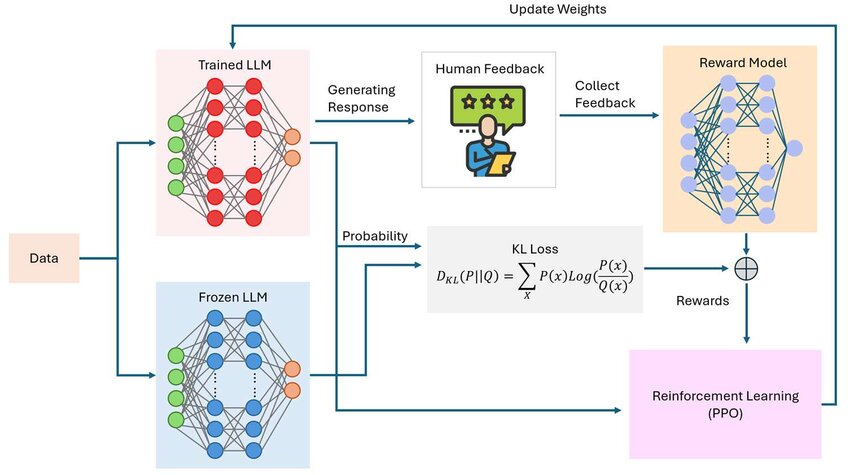
\includegraphics[width=1.0\textwidth]{rlhf_pipeline.png}
    \captionof{figure}{Quy trình ba bước của RLHF: (1) Tinh chỉnh có giám sát (SFT), (2) Huấn luyện Mô hình Phần thưởng (RM), (3) Tối ưu hóa bằng Học tăng cường (PPO).}
    \label{fig:rlhf_pipeline}
\end{center}

\subsubsection{Bước 1: Tinh chỉnh có giám sát (Supervised Fine-Tuning - SFT)}
\begin{itemize}
    \item \textbf{Mục tiêu:} Dạy cho mô hình văn phong và định dạng của một trợ lý đối thoại.
    \item \textbf{Quy trình:} Đây chính là bước \textbf{Instruction Tuning} mà chúng ta đã học ở mục \ref{sec:instruction_tuning}. Một nhóm nhỏ những người gán nhãn chuyên nghiệp (labelers) sẽ viết các prompt chất lượng cao và các câu trả lời mẫu lý tưởng. Mô hình ngôn ngữ cơ sở (base LLM) sau đó được fine-tune trên bộ dữ liệu này.
    \item \textbf{Kết quả:} Một mô hình SFT có khả năng tuân theo chỉ dẫn, nhưng chưa được căn chỉnh sâu về các sở thích tinh tế.
\end{itemize}

\subsubsection{Bước 2: Huấn luyện một Mô hình Phần thưởng (Reward Model - RM)}
Đây là bước cốt lõi của RLHF.
\begin{itemize}
    \item \textbf{Mục tiêu:} Dạy cho một mô hình khác (gọi là Mô hình Phần thưởng) cách \textbf{đánh giá chất lượng} của một câu trả lời, mô phỏng lại sở thích của con người. RM sẽ nhận vào một cặp (prompt, response) và trả về một điểm số duy nhất thể hiện mức độ "tốt" của câu trả lời đó.
    \item \textbf{Quy trình thu thập dữ liệu:}
        \begin{enumerate}
            \item Lấy một prompt từ bộ dữ liệu.
            \item Cho mô hình SFT (từ bước 1) sinh ra nhiều câu trả lời khác nhau (ví dụ: 4 đến 9 câu).
            \item Yêu cầu người gán nhãn \textbf{xếp hạng (rank)} các câu trả lời này từ tốt nhất đến tệ nhất, dựa trên các tiêu chí HHH.
        \end{enumerate}
        Việc yêu cầu con người xếp hạng thay vì cho điểm trực tiếp sẽ dễ dàng và nhất quán hơn nhiều.
    \item \textbf{Quy trình huấn luyện RM:}
        \begin{itemize}
            \item Dữ liệu huấn luyện của RM là các cặp so sánh. Ví dụ, với một prompt, nếu câu trả lời $A$ được xếp hạng cao hơn câu trả lời $B$, chúng ta có một điểm dữ liệu `(prompt, response\_A, response\_B)` với nhãn `A > B`.
            \item RM (thường là một mô hình Encoder-Only như RoBERTa hoặc một LLM đã được loại bỏ lớp cuối) được huấn luyện để dự đoán xác suất một câu trả lời sẽ được con người ưa thích hơn. Cụ thể, nó được huấn luyện để gán một điểm số $r(x, y)$ cho mỗi cặp (prompt $x$, response $y$) sao cho với các cặp được xếp hạng, $r(x, y_{\text{thích hơn}}) > r(x, y_{\text{kém hơn}})$.
        \end{itemize}
    \item \textbf{Kết quả:} Một Mô hình Phần thưởng có khả năng "chấm điểm" bất kỳ câu trả lời nào, hoạt động như một "giám khảo AI" được đào tạo từ sở thích của con người.
\end{itemize}

\subsubsection{Bước 3: Tối ưu hóa bằng Học tăng cường (Reinforcement Learning)}
\begin{itemize}
    \item \textbf{Mục tiêu:} Sử dụng Mô hình Phần thưởng để tinh chỉnh chính sách của mô hình SFT.
    \item \textbf{Thiết lập Học tăng cường (RL):}
        \begin{itemize}
            \item \textbf{Tác tử (Agent):} Chính là mô hình SFT.
            \item \textbf{Chính sách (Policy):} Là chính mô hình SFT, quyết định xác suất sinh ra một token khi biết trạng thái.
            \item \textbf{Không gian hành động (Action Space):} Toàn bộ từ vựng của mô hình.
            \item \textbf{Môi trường (Environment):} Người dùng đưa ra một prompt.
            \item \textbf{Phần thưởng (Reward):} Điểm số được tính bởi \textbf{Mô hình Phần thưởng} (từ bước 2).
        \end{itemize}
    \item \textbf{Quy trình huấn luyện:}
        \begin{enumerate}
            \item Lấy một prompt từ bộ dữ liệu.
            \item Mô hình SFT (chính sách hiện tại) sinh ra một câu trả lời.
            \item Mô hình Phần thưởng chấm điểm câu trả lời này để tạo ra một phần thưởng.
            \item Phần thưởng này được sử dụng làm tín hiệu để cập nhật các trọng số của mô hình SFT thông qua một thuật toán tối ưu hóa chính sách như \textbf{Proximal Policy Optimization (PPO) \cite{schulman2017proximal}}.
            \item Một thành phần quan trọng được thêm vào hàm phần thưởng là một \textbf{hình phạt KL-divergence}. Nó đo lường sự khác biệt giữa chính sách hiện tại và chính sách của mô hình SFT gốc. Hình phạt này ngăn không cho mô hình "tối ưu quá mức" cho Mô hình Phần thưởng và đi quá xa so với những gì nó đã học, giúp nó không bị "quên" các kiến thức ngôn ngữ cơ bản.
        \end{enumerate}
    \item \textbf{Kết quả:} Một mô hình đã được căn chỉnh cuối cùng, có khả năng sinh ra các câu trả lời vừa tuân theo chỉ dẫn, vừa được con người ưa thích.
\end{itemize}

\subsection{Các phương pháp thay thế: Hướng tới sự Đơn giản và Ổn định}
\label{ssec:rlhf_alternatives}
RLHF cực kỳ mạnh mẽ nhưng cũng rất phức tạp, tốn kém và không ổn định để huấn luyện. Điều này đã thúc đẩy việc tìm kiếm các phương pháp thay thế đơn giản hơn.

\subsubsection{Direct Preference Optimization (DPO)}
\begin{itemize}
    \item \textbf{Ý tưởng cốt lõi (Rafailov et al., 2023) \cite{rafailov2023direct}:} Tại sao phải huấn luyện một Mô hình Phần thưởng riêng biệt rồi lại dùng RL để tối ưu hóa nó? Chúng ta có thể tối ưu hóa trực tiếp trên dữ liệu sở thích của con người chỉ bằng một hàm mất mát duy nhất.
    \item \textbf{Cơ chế:} DPO chứng minh rằng hàm mất mát của RLHF có thể được viết lại thành một hàm mất mát đơn giản, có thể được tối ưu hóa trực tiếp bằng cách fine-tuning có giám sát.
    \item \textbf{Quy trình:} DPO chỉ cần dữ liệu so sánh (prompt, câu trả lời được thích hơn, câu trả lời kém hơn) và fine-tune mô hình SFT trực tiếp trên dữ liệu này. Nó tối ưu hóa mô hình để tăng xác suất của các câu trả lời được ưa thích và giảm xác suất của các câu trả lời không được ưa thích, trong khi vẫn duy trì một khoảng cách nhất định với mô hình tham chiếu.
    \item \textbf{Lợi ích:} Đơn giản hơn rất nhiều, ổn định hơn, và thường cho kết quả tương đương hoặc tốt hơn RLHF. DPO đang nhanh chóng trở thành một tiêu chuẩn mới cho việc căn chỉnh.
\end{itemize}

\subsubsection{Constitutional AI (CAI)}
\begin{itemize}
    \item \textbf{Ý tưởng cốt lõi (Bai et al., 2022) \cite{bai2022constitutional}:} Giảm sự phụ thuộc vào phản hồi của con người, đặc biệt là trong việc làm cho mô hình trở nên vô hại. Thay vì yêu cầu con người gán nhãn các nội dung độc hại, hãy để mô hình tự học cách tuân theo một bộ \textbf{"hiến pháp" (constitution)} gồm các nguyên tắc cơ bản.
    \item \textbf{Quy trình (Giai đoạn RL from AI Feedback - RLAIF):}
        \begin{enumerate}
            \item \textbf{Phê bình (Critique):} Cho mô hình SFT xem một prompt có thể gây hại. Yêu cầu chính mô hình (hoặc một mô hình khác) phê bình câu trả lời của nó dựa trên các nguyên tắc trong hiến pháp.
            \item \textbf{Sửa đổi (Revision):} Yêu cầu mô hình viết lại câu trả lời dựa trên những lời phê bình đó để làm cho nó tuân thủ hiến pháp hơn.
            \item \textbf{Huấn luyện:} Cặp (câu trả lời gốc, câu trả lời đã sửa đổi) bây giờ có thể được sử dụng làm dữ liệu sở thích (sửa đổi > gốc) để huấn luyện một Mô hình Phần thưởng hoặc sử dụng DPO.
        \end{enumerate}
    \item \textbf{Lợi ích:} Tự động hóa quá trình tạo dữ liệu căn chỉnh về tính vô hại, giảm bớt gánh nặng và sự phơi nhiễm của con người với các nội dung độc hại.
\end{itemize}

Quá trình căn chỉnh là bước cuối cùng và cũng là một trong những bước phức tạp nhất, biến một công cụ mạnh mẽ thành một đối tác đáng tin cậy.

\bigskip
\hrule
\bigskip

\begin{center}
    \textbf{\Large KẾT THÚC CHƯƠNG 5}
\end{center}

\textit{Chương này đã trang bị cho bạn những kỹ thuật thiết yếu để biến một mô hình nền tảng thô thành một công cụ hữu ích và an toàn. Chúng ta đã đi từ các phương pháp tinh chỉnh kinh điển, đến các kỹ thuật PEFT hiệu quả, và khám phá sức mạnh của việc "trò chuyện" với mô hình thông qua Prompt Engineering. Cuối cùng, chúng ta đã tìm hiểu các quy trình phức tạp như RLHF và DPO để căn chỉnh hành vi của mô hình với sở thích của con người. Với một mô hình đã được tinh chỉnh và căn chỉnh, chúng ta đã có một "bộ não" AI mạnh mẽ. Tuy nhiên, để giải quyết các vấn đề phức tạp trong thế giới thực, bộ não này cần có khả năng truy cập kiến thức bên ngoài, sử dụng công cụ, và thậm chí tương tác với các phương thức khác như hình ảnh. Chương tiếp theo sẽ khám phá các hệ thống và kiến trúc nâng cao kết hợp LLM với các thành phần bên ngoài, tạo ra các ứng dụng AI thực sự toàn diện.}

% \chapter{CÁC KIẾN TRÚC MẠNG NƠ-RON KINH ĐIỂN}
\label{chap:deep_learning_architectures}

Chào mừng bạn đến với kỷ nguyên học sâu của NLP. Trong chương 2, chúng ta đã thấy các mô hình thống kê như N-gram có thể nắm bắt các phụ thuộc cục bộ, nhưng lại bất lực trước các mối quan hệ tầm xa. Cuộc cách mạng word embedding đã cho chúng ta các vector từ mang đầy ngữ nghĩa, nhưng làm thế nào để kết hợp chúng lại nhằm hiểu được ý nghĩa của cả một câu hay một đoạn văn?

Chương này sẽ giới thiệu các kiến trúc mạng nơ-ron nền tảng được thiết kế đặc biệt để xử lý dữ liệu dạng chuỗi như ngôn ngữ tự nhiên. Những kiến trúc này không chỉ đơn thuần "nhìn" vào các từ một cách riêng lẻ, mà còn có khả năng "ghi nhớ" và "lý luận" dựa trên thông tin đã xử lý trước đó, cho phép chúng nắm bắt được ngữ cảnh và các phụ thuộc phức tạp trong câu.
% % !TEX root = ../main.tex
% File: chapters_part1/chap6_1.tex
% Nội dung cho Chương 6, Phần 1


\section{Tìm kiếm và Sinh Tăng cường (Retrieval-Augmented Generation - RAG)}
\label{sec:rag}

\begin{tcolorbox}[
    title=Trực giác cốt lõi của RAG,
    colback=yellow!10!white, colframe=yellow!50!black, fonttitle=\bfseries
]
Thay vì buộc LLM phải "nhớ" mọi thứ, hãy cho nó làm một "bài kiểm tra mở sách" (open-book exam). Khi nhận được một câu hỏi, thay vì trả lời ngay lập tức từ trí nhớ, hệ thống RAG trước hết sẽ \textbf{tìm kiếm (retrieve)} các thông tin liên quan nhất từ một cơ sở tri thức bên ngoài (ví dụ: tài liệu công ty, Wikipedia, các file PDF). Sau đó, nó sẽ cung cấp các thông tin đã tìm được này, cùng với câu hỏi gốc, cho LLM để \textbf{sinh ra (generate)} một câu trả lời dựa trên các bằng chứng đó.
\end{tcolorbox}

RAG biến LLM từ một "nhà hiền triết" biết tuốt (nhưng đôi khi đãng trí và bịa chuyện) thành một "nhà nghiên cứu" tài ba, có khả năng tìm kiếm, tổng hợp và trả lời dựa trên các nguồn thông tin xác thực.

\subsection{Tại sao và Khi nào chúng ta cần RAG?}
\label{ssec:why_rag}
Trước khi đi sâu vào kỹ thuật, điều quan trọng là phải hiểu rõ các vấn đề mà RAG giải quyết và khi nào nó là công cụ phù hợp.

\paragraph{Các vấn đề cố hữu của LLM}
Các mô hình ngôn ngữ lớn, dù mạnh mẽ đến đâu, vẫn đối mặt với ba thách thức lớn:
\begin{itemize}
    \item \textbf{Bịa đặt thông tin (Hallucination):} LLM có xu hướng tự "sáng tạo" ra các thông tin không có thật một cách rất tự tin, gây ra rủi ro nghiêm trọng trong các ứng dụng đòi hỏi tính chính xác.
    \item \textbf{Giới hạn tri thức (Knowledge Cutoff):} Tri thức của LLM bị đóng băng tại thời điểm nó được huấn luyện. Nó không biết về các sự kiện, dữ liệu hoặc thông tin mới xuất hiện sau ngày đó.
    \item \textbf{Thiếu tính kiểm chứng (Lack of Verifiability):} Khi LLM đưa ra một câu trả lời, rất khó để truy ngược lại nguồn thông tin mà nó đã sử dụng, khiến việc xác thực trở nên bất khả thi.
\end{itemize}
RAG được thiết kế để giải quyết trực tiếp cả ba vấn đề này bằng cách cung cấp cho LLM các bằng chứng cập nhật và có thể kiểm chứng tại thời điểm trả lời.

\paragraph{Khi nào nên sử dụng RAG?}
\begin{itemize}
    \item Khi ứng dụng của bạn cần truy cập vào \textbf{kho tri thức riêng tư, lớn, hoặc thay đổi liên tục} (tài liệu nội bộ, cơ sở dữ liệu sản phẩm, văn bản pháp luật mới). Việc fine-tune lại LLM liên tục là không khả thi và tốn kém.
    \item Khi \textbf{tính chính xác và khả năng trích dẫn nguồn} là yêu cầu bắt buộc (trợ lý pháp lý, tư vấn y tế, tra cứu thông tin tài chính).
    \item Khi mục tiêu chính là \textbf{giảm thiểu rủi ro bịa đặt thông tin} và đảm bảo câu trả lời được neo vào các nguồn xác thực.
\end{itemize}

\subsection{Kiến trúc RAG Cơ bản (The Naive RAG Pipeline)}
\label{ssec:naive_rag}
Một hệ thống RAG cơ bản, thường được gọi là "Naive" hay "Vanilla" RAG, bao gồm hai giai đoạn chính: \textbf{Lập chỉ mục (Indexing)} và \textbf{Truy vấn (Querying)}. Đây là nền tảng để hiểu tất cả các kỹ thuật nâng cao sau này.

\paragraph{Giai đoạn 1: Lập chỉ mục (Offline)}
Giai đoạn này được thực hiện một lần hoặc định kỳ để chuẩn bị cơ sở tri thức. Nó giống như việc chúng ta sắp xếp và tạo mục lục cho một thư viện.
\begin{enumerate}
    \item \textbf{Tải Dữ liệu (Load):} Tải các tài liệu từ nguồn (PDF, TXT, HTML, v.v.).
    \item \textbf{Phân mảnh (Chunk/Split):} Chia các tài liệu dài thành các đoạn nhỏ hơn, gọi là các "chunk". Trong kiến trúc cơ bản, đây thường là \textit{fixed-size chunking} (chia thành các đoạn có kích thước cố định).
    \item \textbf{Nhúng (Embed):} Sử dụng một mô hình nhúng (embedding model, ví dụ: các bi-encoder từ `sentence-transformers`) để chuyển mỗi chunk thành một vector số (embedding). Vector này nắm bắt ngữ nghĩa của chunk đó.
    \item \textbf{Lưu trữ (Store):} Lưu trữ các chunk và các vector embedding tương ứng của chúng vào một \textbf{Cơ sở dữ liệu Vector} (Vector Database) như FAISS, ChromaDB, hoặc pgvector.
\end{enumerate}

\paragraph{Giai đoạn 2: Truy vấn (Online)}
Giai đoạn này xảy ra mỗi khi người dùng đặt câu hỏi.
\begin{enumerate}
    \item \textbf{Nhúng Câu hỏi (Query Embedding):} Câu hỏi của người dùng được nhúng thành một vector truy vấn, sử dụng \textbf{cùng một embedding model} đã dùng ở giai đoạn lập chỉ mục.
    \item \textbf{Tìm kiếm (Retrieve):} Vector truy vấn được sử dụng để thực hiện một \textit{tìm kiếm tương đồng (similarity search)} trong Vector Database, nhằm tìm ra $k$ chunk có vector gần nhất (tương đồng nhất về mặt ngữ nghĩa).
    \item \textbf{Tăng cường Prompt (Augment):} Các chunk đã tìm được được ghép vào prompt cùng với câu hỏi gốc của người dùng.
        \begin{tcolorbox}[colback=gray!5!white, colframe=gray!50!black, sharp corners]
        \textbf{Ngữ cảnh được cung cấp:} \\
        \textit{[Nội dung của chunk 1...]} \\
        \textit{[Nội dung của chunk 2...]} \\
        \textit{[...]} \\
        \textbf{Dựa vào ngữ cảnh trên, hãy trả lời câu hỏi sau:} \\
        \textit{[Câu hỏi gốc của người dùng]} \\
        \textbf{Trả lời:}
        \end{tcolorbox}
    \item \textbf{Sinh Câu trả lời (Generate):} Prompt đã được tăng cường này được gửi đến một LLM. LLM sẽ tổng hợp thông tin từ ngữ cảnh được cung cấp để tạo ra câu trả lời cuối cùng.
\end{enumerate}

\begin{center}
    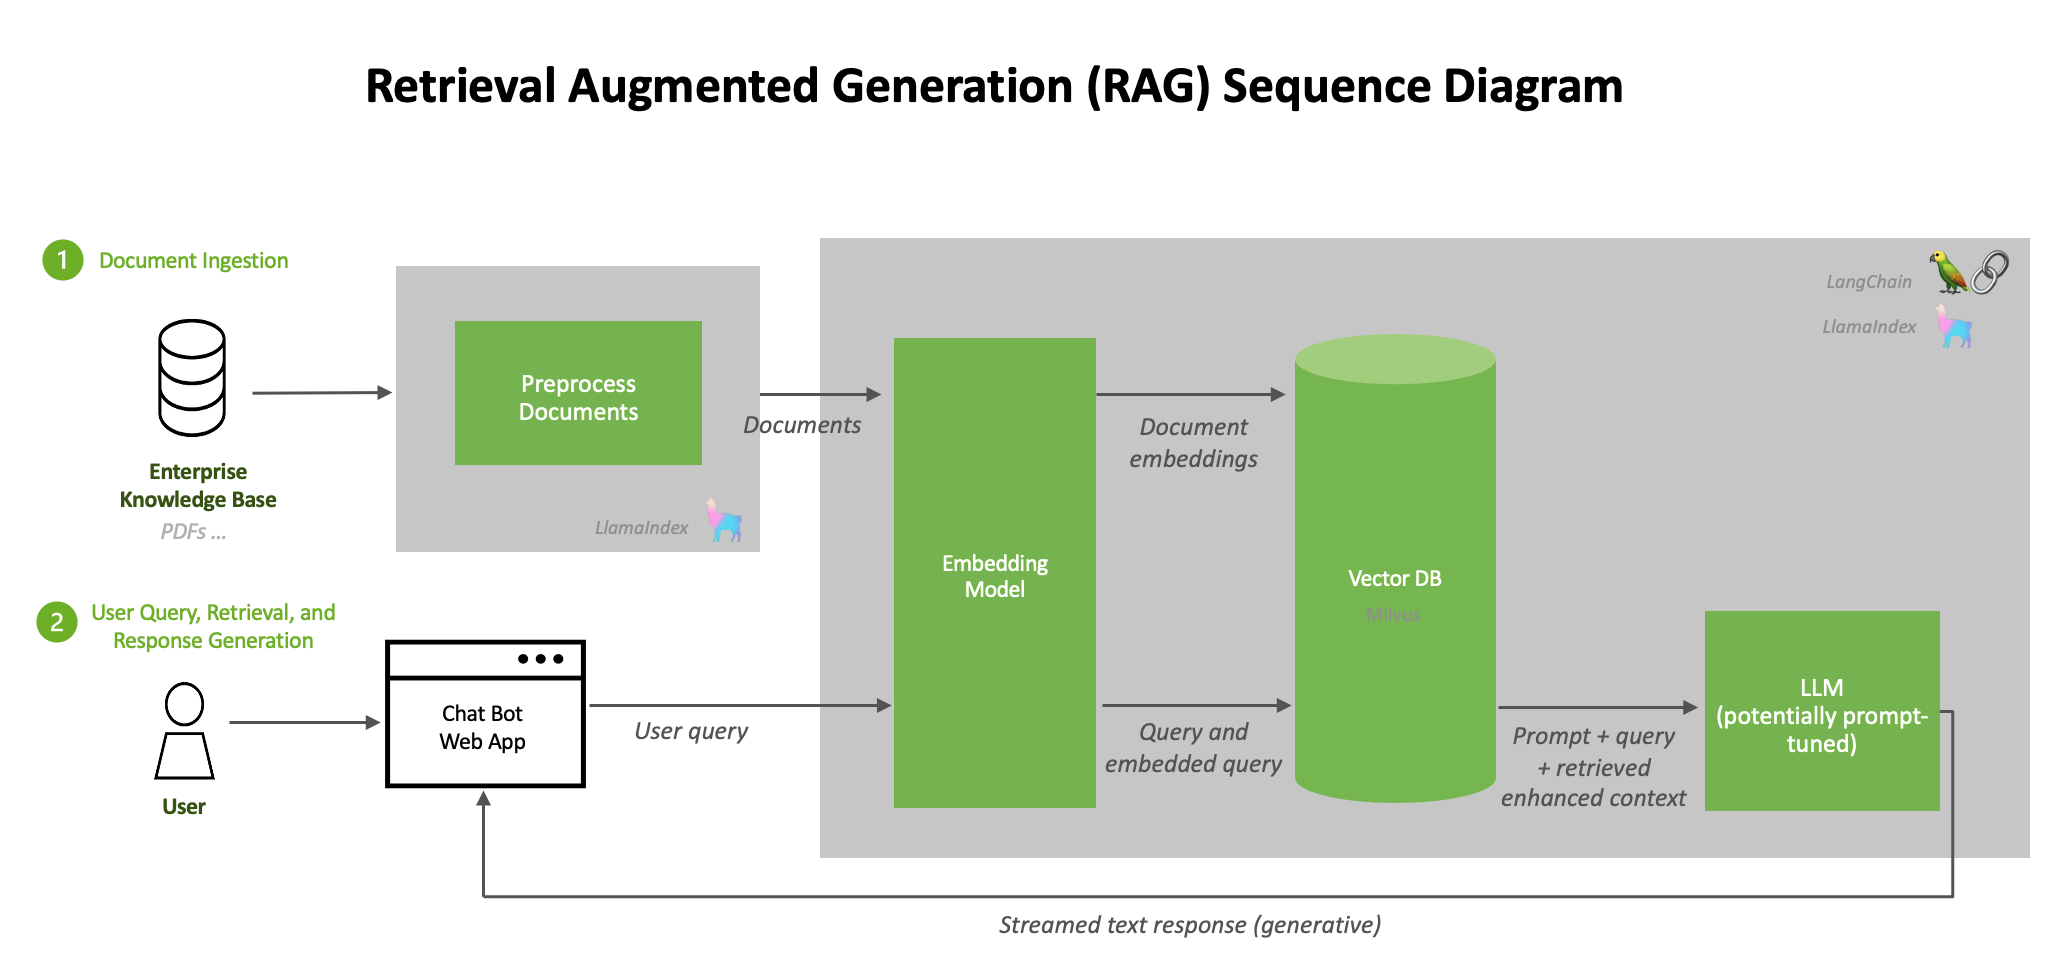
\includegraphics[width=1.0\textwidth]{rag_pipeline_diagram.png}
    \captionof{figure}{Sơ đồ kiến trúc của một hệ thống RAG, bao gồm giai đoạn Lập chỉ mục (bên trên) và giai đoạn Truy vấn (bên dưới).}
    \label{fig:rag_pipeline_diagram}
\end{center}

\subsection{Bài học từ các Công cụ Tìm kiếm: Kiến trúc Phân tầng của Google}
\label{ssec:lesson_from_google}
Để hiểu tại sao các hệ thống RAG hiện đại được thiết kế theo một cách cụ thể, sẽ rất hữu ích khi nhìn vào "người khổng lồ" trong lĩnh vực tìm kiếm: Google. Kiến trúc của Google Search là một ví dụ điển hình về một hệ thống retrieval đa tầng (multi-stage), nơi mỗi tầng sẽ lọc và tinh chỉnh kết quả, cân bằng giữa tốc độ và độ chính xác.

\paragraph{Kiến trúc Phân tầng (A Tiered Architecture)}
Một truy vấn trên Google không chỉ đơn giản là "tìm và trả về". Nó đi qua một "phễu" tinh vi gồm nhiều giai đoạn:
\begin{enumerate}
    \item \textbf{Crawl \& Indexing (Thu thập và Lập chỉ mục):} 
    Trước khi bất kỳ truy vấn nào được xử lý, Googlebot liên tục \emph{crawl} web, tải về nội dung và phân tích cấu trúc trang. Dữ liệu sau đó được chuẩn hoá và lưu trong nhiều loại chỉ mục:
    \begin{itemize}
        \item \emph{Inverted Index (Sparse Index):} ánh xạ từ khoá $\rightarrow$ danh sách tài liệu chứa từ đó.
        \item \emph{Dense Index (Vector Index):} biểu diễn văn bản dưới dạng embedding để phục vụ tìm kiếm ngữ nghĩa.
        \item Ngoài ra, các siêu dữ liệu (metadata), đồ thị liên kết (PageRank), và thông tin đa phương tiện (hình ảnh, video) cũng được lưu trữ song song.
    \end{itemize}

    \item \textbf{Query Understanding (Hiểu Truy vấn):} 
    Khi người dùng nhập một truy vấn, Google áp dụng các mô hình ngôn ngữ tiên tiến (BERT, MUM, T5) để phân tích ý định và ngữ nghĩa. Các bước xử lý điển hình gồm:
    \begin{itemize}
        \item Chuẩn hoá, sửa lỗi chính tả, mở rộng từ đồng nghĩa.
        \item Nhận diện thực thể (entity recognition) và giải quyết nhập nhằng (disambiguation).
        \item Viết lại truy vấn (query rewriting) và cá nhân hoá dựa trên ngôn ngữ, vị trí, lịch sử tìm kiếm.
    \end{itemize}

    \item \textbf{Candidate Generation (Tạo Ứng viên - Nhanh và Rộng):}
    \begin{itemize}
        \item \textbf{Mục tiêu:} Từ hàng tỷ tài liệu, nhanh chóng lọc ra một tập hợp lớn (10,000--100,000) ứng viên tiềm năng.
        \item \textbf{Công nghệ:} Kết hợp \emph{Sparse Retrieval} (BM25/TF-IDF) với \emph{Dense Retrieval} (bi-encoders + ANN search). Giai đoạn này ưu tiên \textbf{Recall} --- đảm bảo không bỏ sót kết quả quan trọng.
    \end{itemize}

    \item \textbf{Initial Ranking (Xếp hạng ban đầu):}
    \begin{itemize}
        \item \textbf{Mục tiêu:} Thu hẹp tập ứng viên từ hàng chục nghìn xuống còn vài nghìn tài liệu có triển vọng.
        \item \textbf{Công nghệ:} Sử dụng \emph{Learning-to-Rank models} (boosted trees, shallow neural nets) để kết hợp nhiều tín hiệu: điểm BM25, PageRank, độ mới (freshness), anchor text, độ phổ biến của tài liệu. Đây là lớp lọc trung gian quan trọng trước khi áp dụng mô hình ngôn ngữ nặng nề.
    \end{itemize}

    \item \textbf{Neural Re-ranking \& Final Touches (Xếp hạng lại bằng mô hình Neural và Tinh chỉnh cuối cùng):}
    \begin{itemize}
        \item \textbf{Mục tiêu:} Đạt độ chính xác cao nhất trong top kết quả hiển thị (thường là vài chục link).
        \item \textbf{Công nghệ:} Các \emph{Cross-Encoders} hoặc mô hình seq2seq (như T5, BERT, MUM) được áp dụng cho vài trăm ứng viên. Các mô hình này đánh giá trực tiếp cặp \emph{(truy vấn, tài liệu)} nên rất chính xác, dù tốn kém về tính toán.
        \item \textbf{Tinh chỉnh cuối cùng:} Diversification (đa dạng hoá kết quả), lọc spam, tích hợp Knowledge Graph, snippet, và kết hợp các nguồn media (tin tức, hình ảnh, video).
        \item Ngoài ra, các tín hiệu hành vi người dùng (CTR, dwell time) được khai thác để điều chỉnh thứ hạng theo thời gian.
    \end{itemize}
\end{enumerate}

\begin{tcolorbox}[
    title=Bài học cốt lõi cho RAG từ Google,
    colback=green!5!white, colframe=green!60!black, fonttitle=\bfseries
]
Xây dựng một hệ thống retrieval mạnh mẽ không phải là việc chọn một thuật toán duy nhất. Đó là việc xây dựng một \textbf{pipeline đa tầng}. Chúng ta chấp nhận sử dụng các phương pháp "đủ tốt" và nhanh ở giai đoạn đầu để lọc số lượng lớn, sau đó mới đầu tư tài nguyên tính toán vào các phương pháp chính xác cao cho một số lượng nhỏ các ứng viên hứa hẹn nhất. Triết lý "lọc rộng rồi tinh chỉnh sâu" này chính là nền tảng cho các hệ thống RAG hiện đại.
\end{tcolorbox}

\subsection{Tối ưu hóa Giai đoạn 1: Lập chỉ mục Thông minh (Smarter Indexing)}
\label{ssec:smarter_indexing}
Chất lượng của các chunk được lập chỉ mục ảnh hưởng trực tiếp đến khả năng tìm thấy thông tin chính xác. "Rác vào, Rác ra". Các kỹ thuật dưới đây giúp cải thiện "chất lượng đầu vào" cho hệ thống RAG.

\subsubsection{Chiến lược Phân mảnh Nâng cao (Advanced Chunking Strategies)}
Việc chia văn bản một cách "mù quáng" theo kích thước cố định (fixed-size chunking) thường làm phá vỡ ngữ nghĩa của câu hoặc đoạn văn.
\begin{itemize}
    \item \textbf{Chunking theo Ngữ nghĩa/Cấu trúc (Semantic/Structural Chunking):} Thay vì chia theo số ký tự, chúng ta chia dựa trên các ranh giới tự nhiên của văn bản như dấu ngắt câu, đoạn văn, tiêu đề (Markdown headers), hoặc các thẻ HTML. Điều này giúp các chunk giữ được sự mạch lạc và trọn vẹn về ý nghĩa.
    \item \textbf{Chunking có chồng lấn (Overlap Chunking):} Để tránh mất ngữ cảnh ở điểm nối giữa hai chunk, một phần nhỏ của chunk trước được lặp lại ở đầu chunk sau. Ví dụ: chunk 1 chứa các câu [1, 2, 3, 4], chunk 2 sẽ chứa các câu [4, 5, 6, 7].
\end{itemize}

\subsubsection{Kỹ thuật Small-to-Big và Sentence-Windowing}
Đây là một kỹ thuật mạnh mẽ để cân bằng giữa độ chính xác khi tìm kiếm và đầy đủ ngữ cảnh cho LLM.
\begin{itemize}
    \item \textbf{Vấn đề:} Các chunk lớn (nguyên đoạn văn) chứa nhiều ngữ cảnh nhưng khó khớp chính xác với một câu hỏi cụ thể. Các chunk nhỏ (một câu) thì dễ khớp chính xác nhưng lại thiếu ngữ cảnh xung quanh.
    \item \textbf{Giải pháp "Small-to-Big":}
    \begin{enumerate}
        \item \textbf{Lập chỉ mục (Index):} Chia tài liệu thành các đơn vị nhỏ (ví dụ: từng câu) và nhúng chúng.
        \item \textbf{Tìm kiếm (Retrieve):} Tìm kiếm trên các câu đơn lẻ để có độ chính xác cao nhất.
        \item \textbf{Mở rộng (Expand):} Sau khi tìm được câu phù hợp nhất, thay vì chỉ trả về câu đó, hệ thống sẽ lấy ra một "cửa sổ" văn bản lớn hơn xung quanh câu đó (ví dụ: 3 câu trước và 3 câu sau, hoặc toàn bộ đoạn văn chứa câu đó) để cung cấp cho LLM.
    \end{enumerate}
    Kỹ thuật này giúp đạt được \textit{sự chính xác trong tìm kiếm} và \textit{sự đầy đủ về ngữ cảnh} khi sinh câu trả lời.
\end{itemize}

\subsubsection{Tầm quan trọng của Metadata}
Metadata là "thông tin về thông tin". Khi lập chỉ mục, việc lưu trữ metadata cùng với mỗi chunk là cực kỳ quan trọng cho các ứng dụng thực tế.
\begin{itemize}
    \item \textbf{Ví dụ về Metadata:} Tên file nguồn, số trang, ngày xuất bản, tác giả, tiêu đề chương/mục, URL.
    \item \textbf{Tại sao nó quan trọng?}
    \begin{itemize}
        \item \textbf{Trích dẫn nguồn:} Giúp LLM có thể trích dẫn nguồn gốc của thông tin một cách chính xác trong câu trả lời (ví dụ: "Theo tài liệu X, trang 5...").
        \item \textbf{Lọc trước khi tìm kiếm (Pre-filtering):} Cho phép thu hẹp không gian tìm kiếm. Ví dụ: "Chỉ tìm kiếm trong các tài liệu được xuất bản sau năm 2023".
        \item \textbf{Gỡ lỗi (Debugging):} Dễ dàng truy vết xem chunk gây ra câu trả lời sai đến từ tài liệu nào.
    \end{itemize}
\end{itemize}

\subsection{Tối ưu hóa Giai đoạn 2: Tìm kiếm và Xếp hạng (Advanced Retrieval \& Ranking)}
\label{ssec:advanced_retrieval_ranking}
\begin{tcolorbox}[title=Mục tiêu, colback=blue!5!white, colframe=blue!75!black]
Retriever là trái tim của RAG. Giai đoạn này quyết định "chất lượng nguyên liệu đầu vào" cho LLM. Một hệ thống RAG chỉ có thể tốt bằng thành phần retriever của nó. Các kỹ thuật dưới đây giúp tìm được những mảnh ghép thông tin (chunk) chính xác, liên quan và đa dạng nhất.
\end{tcolorbox}

\subsection{Tối ưu hóa Giai đoạn 2: Tìm kiếm và Xếp hạng (Advanced Retrieval \& Ranking)}
\label{ssec:advanced_retrieval_ranking_refactored}
Lấy cảm hứng từ kiến trúc của Google, giờ đây chúng ta sẽ áp dụng triết lý đa tầng vào hệ thống RAG của mình.

\subsubsection{Tìm kiếm Lai (Hybrid Search): Giai đoạn Candidate Generation của RAG}
Đây chính là giai đoạn 1 của chúng ta. Thay vì chỉ dùng một phương pháp, ta kết hợp cả hai:
\begin{itemize}
    \item \textbf{Cơ chế:} Hệ thống chạy song song cả Sparse Retriever (BM25) và Dense Retriever (Vector Search). Sau đó, điểm số từ hai hệ thống được kết hợp lại (ví dụ: dùng thuật toán Reciprocal Rank Fusion - RRF) để tạo ra một danh sách ứng viên (candidate list) chất lượng cao.
    \item \textbf{Lợi ích:} Tận dụng khả năng khớp từ khóa chính xác của Sparse và khả năng hiểu ngữ nghĩa sâu sắc của Dense. Đây được coi là phương pháp mặc định để có được recall tốt nhất.
\end{itemize}

\subsubsection{Xếp hạng lại (Re-ranking) với Cross-Encoders}
\begin{itemize}
    \item \textbf{Vấn đề:} Hybrid Search rất nhanh và hiệu quả để lọc ra top 100-200 ứng cử viên tiềm năng từ hàng triệu chunk. Nhưng trong top 100 này, đâu mới là những chunk thực sự tốt nhất?
    \item \textbf{Giải pháp:} Sử dụng một mô hình thứ hai, mạnh hơn nhưng chậm hơn, gọi là \textbf{Cross-Encoder}.
        \begin{itemize}
            \item \textbf{Cơ chế:} Thay vì tạo vector riêng cho câu hỏi và tài liệu, Cross-Encoder nhận vào cặp \texttt{(câu hỏi, chunk)} và đưa ra một điểm số tương đồng duy nhất. Việc xem xét cả hai cùng lúc cho phép nó hiểu được sự tương tác tinh vi hơn.
            \item \textbf{Quy trình:} Hybrid Search tìm ra top-K ứng viên (K lớn). Sau đó, Cross-Encoder sẽ đánh giá và xếp hạng lại top-K này để chọn ra top-N cuối cùng (N nhỏ) gửi cho LLM.
        \end{itemize}
\end{itemize}

\subsection{Tối ưu hóa Giai đoạn 3: Tăng cường và Sinh (Smarter Augmentation \& Generation)}
\label{ssec:smarter_aug_gen}
Sau khi đã có những chunk chất lượng nhất, chúng ta cần đảm bảo chúng được sử dụng một cách hiệu quả và trung thực.

\subsubsection{Nén Ngữ cảnh (Context Compression)}
Đôi khi, các chunk được tìm thấy vẫn chứa nhiều thông tin thừa so với câu hỏi. Việc "nhồi nhét" tất cả vào prompt có thể làm LLM bị nhiễu.
\begin{itemize}
    \item \textbf{Cơ chế:} Trước khi đưa các chunk vào prompt cuối cùng, một mô hình nhỏ hơn sẽ chạy qua và chỉ giữ lại những câu, những ý có liên quan trực tiếp đến câu hỏi của người dùng.
    \item \textbf{Lợi ích:} Giảm độ dài của prompt (tiết kiệm chi phí), tăng sự tập trung cho LLM vào các bằng chứng quan trọng nhất.
\end{itemize}

\subsubsection{Kiểm soát việc Sinh: Buộc Trích dẫn và Chống Bịa đặt (Hallucination Guardrails)}
Đây là bước cuối cùng và quan trọng nhất để đảm bảo tính tin cậy.
\begin{itemize}
    \item \textbf{Instruction Tuning:} Huấn luyện hoặc chỉ dẫn LLM một cách rõ ràng thông qua prompt: \textit{"Hãy trả lời câu hỏi chỉ dựa trên ngữ cảnh được cung cấp. Với mỗi thông tin đưa ra, hãy trích dẫn nguồn [doc\_id, chunk\_id]. Nếu thông tin không có trong ngữ cảnh, hãy trả lời 'Tôi không tìm thấy thông tin trong tài liệu'."}
    \item \textbf{Giảm Temperature:} Khi sinh câu trả lời, đặt tham số `temperature` của LLM ở mức thấp (ví dụ: 0.1) để giảm tính ngẫu nhiên và sáng tạo, buộc nó bám sát vào văn bản nguồn.
\end{itemize}

\subsection{Các Mô hình RAG Nâng cao (Advanced RAG Patterns)}
\label{ssec:advanced_rag_patterns}
Khi các bài toán trở nên phức tạp hơn, chúng ta cần các kiến trúc RAG tinh vi hơn.

\begin{itemize}
    \item \textbf{Biến đổi Truy vấn (Query Transformation):} Câu hỏi của người dùng thường không phải là dạng tốt nhất để tìm kiếm. Các kỹ thuật này sẽ biến đổi nó trước:
        \begin{itemize}
        \item \textbf{Viết lại Truy vấn (Query Rewriting):} Là nhóm kỹ thuật tập trung vào việc sửa đổi, mở rộng, hoặc diễn đạt lại văn bản câu hỏi gốc mà không làm thay đổi ý định tìm kiếm cốt lõi. Mục tiêu là cải thiện sự tương thích giữa từ vựng của người dùng và từ vựng trong kho tài liệu, qua đó tăng cả \textit{recall} và \textit{precision}. Các phương pháp này được chia thành ba hướng tiếp cận chính:
    
        \begin{itemize}
            \item \textbf{Viết lại dựa trên Từ vựng (Lexical Rewriting):} 
            Các phương pháp này hoạt động ở cấp độ từ hoặc ký tự, dựa trên các quy tắc, từ điển, hoặc các chuẩn hóa ngôn ngữ cơ bản.
            \begin{itemize}
                \item \textbf{Mở rộng Từ đồng nghĩa (Synonym/Thesaurus Expansion):} Bổ sung các từ hoặc cụm từ đồng nghĩa (ví dụ: \texttt{luật pháp} $\rightarrow$ \texttt{pháp luật}, \texttt{quy định}) để tăng khả năng khớp, giúp bắt được các tài liệu sử dụng cách diễn đạt khác nhau.
                \item \textbf{Chuẩn hóa Hình thái học (Morphological Normalization):} Đưa các biến thể của một từ về dạng gốc (stemming hoặc lemmatization). Ví dụ: các từ \texttt{xử lý}, \texttt{được xử lý}, \texttt{sự xử lý} đều được đưa về gốc \texttt{xử lý}.
                \item \textbf{Sửa lỗi Chính tả/Gõ nhầm (Spelling/Typo Correction):} Tự động phát hiện và sửa các lỗi sai trong truy vấn (\texttt{luật lao đông} $\rightarrow$ \texttt{luật lao động}) để tránh tìm kiếm thất bại.
                \item \textbf{Mở rộng Từ viết tắt (Abbreviation Expansion):} Chuyển các từ viết tắt thành dạng đầy đủ của chúng (ví dụ: \texttt{TP.HCM} $\rightarrow$ \texttt{Thành phố Hồ Chí Minh}, \texttt{LHQ} $\rightarrow$ \texttt{Liên Hợp Quốc}).
                \item \textbf{Xử lý Stopword (Stopword Handling):} Loại bỏ các từ phổ biến, ít mang nghĩa (như \texttt{là}, \texttt{của}, \texttt{và}) để tập trung vào từ khóa chính, hoặc ngược lại, giữ lại chúng khi cần thiết cho các truy vấn yêu cầu sự chính xác về ngữ pháp (phrase queries).
            \end{itemize}
    
            \item \textbf{Viết lại dựa trên Thống kê (Statistical Rewriting):} 
            Các kỹ thuật này tận dụng thông tin thống kê từ kho tài liệu hoặc từ kết quả tìm kiếm ban đầu để mở rộng truy vấn một cách tự động.
            \begin{itemize}
                \item \textbf{Phản hồi Giả liên quan (Pseudo-Relevance Feedback - PRF):} Giả định rằng các tài liệu top-k trong kết quả tìm kiếm ban đầu là liên quan. Hệ thống sẽ trích xuất các thuật ngữ quan trọng từ các tài liệu này để bổ sung vào truy vấn gốc và thực hiện tìm kiếm lại. (Các thuật toán tiêu biểu: Rocchio, RM3).
                \item \textbf{Mở rộng dựa trên Tần suất Cùng xuất hiện (Term Co-occurrence Expansion):} Tìm và thêm vào truy vấn các thuật ngữ thường xuyên xuất hiện cùng với các thuật ngữ gốc trong toàn bộ kho tài liệu (Dựa trên các độ đo như Pointwise Mutual Information - PMI).
                \item \textbf{Mở rộng dựa trên Mô hình Chủ đề (Topic-Model-Based Expansion):} Sử dụng các mô hình như LDA (Latent Dirichlet Allocation) để xác định các chủ đề chính của truy vấn, sau đó bổ sung các từ khóa đặc trưng của những chủ đề đó.
                \item \textbf{Mô hình Liên quan (Relevance Models):} Ước tính một mô hình xác suất của các thuật ngữ sẽ xuất hiện trong một tài liệu liên quan, sau đó lấy mẫu từ mô hình này để tạo ra truy vấn mới.
            \end{itemize}
            
            \item \textbf{Viết lại dựa trên Ngữ nghĩa (Semantic Rewriting):} 
            Các phương pháp hiện đại, tập trung vào việc nắm bắt và mở rộng ý nghĩa, ngữ cảnh của truy vấn thay vì chỉ dựa trên từ vựng bề mặt.
            \begin{itemize}
                \item \textbf{Dựa trên Vector Embedding (Embedding-based Nearest Neighbors):} Biểu diễn truy vấn dưới dạng vector và tìm các từ/cụm từ có vector gần nhất trong không gian embedding để mở rộng (Ví dụ: sử dụng Word2Vec, GloVe, fastText).
                \item \textbf{Diễn đạt lại bằng LLM (LLM-based Paraphrasing):} Sử dụng các mô hình ngôn ngữ lớn (LLM) như GPT-4 hay T5 để tạo ra một phiên bản câu hỏi hoàn toàn mới nhưng giữ nguyên ý nghĩa, giúp vượt qua rào cản từ vựng.
                \item \textbf{Tạo nhiều Truy vấn song song (Multi-Query Rewriting):} Yêu cầu LLM sinh ra nhiều biến thể khác nhau của câu hỏi gốc. Hệ thống sẽ thực hiện tìm kiếm với tất cả các biến thể này và tổng hợp kết quả.
                \item \textbf{Mở rộng bằng Đồ thị Tri thức (Knowledge-Graph Expansion):} Liên kết các thực thể trong truy vấn (tên người, địa điểm, tổ chức) với một đồ thị tri thức. Sau đó, mở rộng truy vấn bằng cách thêm vào các thông tin, thuộc tính, hoặc các thực thể liên quan được lấy từ đồ thị.
                \item \textbf{Mở rộng theo Ngữ cảnh Hội thoại (Contextual Expansion):} Tận dụng lịch sử của cuộc trò chuyện để làm rõ và bổ sung thông tin cho truy vấn hiện tại. Ví dụ, câu hỏi "còn anh ấy thì sao?" sẽ được mở rộng với thông tin về "anh ấy" đã được đề cập trước đó.
            \end{itemize}
        \end{itemize}
        \item \textbf{Biến đổi Biểu diễn Truy vấn (Query Representation Transformation):} Khác với việc viết lại văn bản, nhóm kỹ thuật này giữ nguyên câu hỏi gốc nhưng biến đổi cách nó được \textit{biểu diễn} (thường là dưới dạng vector) để tối ưu hóa việc so khớp trong không gian embedding.
        \begin{itemize}
            \item \textbf{HyDE (Hypothetical Document Embeddings):} 
            Một kỹ thuật đột phá, yêu cầu LLM tự sinh một tài liệu trả lời \textit{giả định} cho câu hỏi. Thay vì nhúng vector của câu hỏi ngắn gọn và thiếu ngữ cảnh, hệ thống sẽ nhúng vector của tài liệu giả định này. Vector này thường giàu thông tin và nằm gần các tài liệu liên quan thực tế trong không gian embedding, do đó cải thiện đáng kể chất lượng tìm kiếm.
            
            \item \textbf{Query2Doc (Q2D):} 
            Một phương pháp tiền thân của HyDE, cũng biến đổi truy vấn thành một dạng trông giống tài liệu hơn, nhưng thường sử dụng các phương pháp heuristic hoặc các mô hình sinh văn bản gọn nhẹ (như T5) thay vì các LLM lớn.
            
            \item \textbf{Tăng cường Embedding Truy vấn (Query Embedding Augmentation):} 
            Cải thiện vector truy vấn gốc bằng cách kết hợp nó với các thông tin bổ sung.
            \begin{itemize}
                \item \textbf{Pooling với các Mở rộng (Average Pooling with Expansions):} 
                Tạo embedding cho truy vấn gốc và các phiên bản mở rộng (ví dụ: từ đồng nghĩa), sau đó kết hợp chúng lại (ví dụ: lấy trung bình) để tạo ra một vector đại diện toàn diện hơn.
                \item \textbf{Hợp nhất Embedding (Embedding Fusion):} 
                Thực hiện tìm kiếm song song với nhiều hệ thống retriever (ví dụ: một sparse retriever như BM25 và một dense retriever). Sau đó, vector truy vấn cuối cùng được điều chỉnh hoặc kết hợp dựa trên thông tin từ các kết quả tìm kiếm này.
            \end{itemize}
            
            \item \textbf{Biểu diễn Truy vấn Tương phản (Contrastive Query Representation):} 
            Tinh chỉnh (fine-tune) mô hình encoder để nó học được cách tạo ra các embedding tốt hơn. Cụ thể, mô hình được huấn luyện để vector của truy vấn gần với vector của tài liệu trả lời đúng (positive sample) và xa các tài liệu không liên quan (negative samples).
            
            \item \textbf{Biến đổi Ngầm định qua Kiến trúc (Implicit Transformation via Architecture):} 
            Một số kiến trúc retriever không tạo ra một vector duy nhất cho truy vấn. Thay vào đó, chúng thực hiện một sự biến đổi ngầm thông qua tương tác sâu hơn giữa truy vấn và tài liệu.
            \begin{itemize}
                \item \textbf{ColBERT (Late Interaction):} 
                Mô hình này tạo ra embedding cho mỗi token trong cả truy vấn và tài liệu. Quá trình so khớp tính toán điểm tương đồng giữa mỗi token của truy vấn với tất cả các token của tài liệu, cho phép một sự tương tác chi tiết và linh hoạt hơn là so khớp hai vector đơn lẻ.
            \end{itemize}
        \end{itemize}
    
        \item \textbf{Phân tích và Cấu trúc hóa Truy vấn (Query Understanding \& Structuring):} Nhóm kỹ thuật này không chỉ "hiểu" ý định của truy vấn mà còn "dịch" nó thành một định dạng có cấu trúc, cho phép tìm kiếm chính xác trên các nguồn dữ liệu có schema rõ ràng (structured/semi-structured data) như cơ sở dữ liệu hoặc kho tri thức.
        \begin{itemize}
            \item \textbf{Tự truy vấn (Self-Querying):} 
            LLM được cung cấp thông tin về siêu dữ liệu (metadata) của kho tài liệu (ví dụ: \texttt{năm xuất bản}, \texttt{tác giả}, \texttt{thể loại}). Khi nhận câu hỏi, LLM tự động phân tích và trích xuất các bộ lọc tương ứng. Ví dụ, câu hỏi "các bài báo của Hinton về mạng nơ-ron sau 2015" sẽ được dịch thành một truy vấn tìm kiếm nội dung "mạng nơ-ron" kèm theo hai bộ lọc: \texttt{tác giả = "Hinton"} và \texttt{năm > 2015}.
            
            \item \textbf{Phân tích Ngữ nghĩa (Semantic Parsing):} 
            Chuyển đổi hoàn toàn câu hỏi ngôn ngữ tự nhiên thành một truy vấn trong một ngôn ngữ truy vấn chính thức như SQL (cho cơ sở dữ liệu quan hệ), SPARQL (cho đồ thị tri thức), hoặc GraphQL.
            
            \item \textbf{Phân rã Truy vấn (Query Decomposition / Multi-Hop):} 
            Đối với các câu hỏi phức tạp đòi hỏi phải kết hợp thông tin từ nhiều nguồn, kỹ thuật này chia câu hỏi lớn thành một chuỗi các câu hỏi con đơn giản hơn. Kết quả của câu hỏi con trước được dùng làm đầu vào cho câu hỏi con tiếp theo.
            
            \item \textbf{Phân định Nghĩa (Query Disambiguation):} 
            Xác định ý nghĩa chính xác của các từ đa nghĩa dựa trên ngữ cảnh. Ví dụ, hệ thống cần phân biệt "Apple" là công ty công nghệ hay là một loại trái cây để có thể tìm kiếm đúng hướng.
            
            \item \textbf{Phân loại Ý định và Trích xuất Thực thể (Intent Classification \& Slot Filling):} 
            Một cách tiếp cận phổ biến trong các hệ thống chatbot, trong đó hệ thống xác định mục đích chung của người dùng (intent) và trích xuất các thông tin chi tiết (entities/slots). Ví dụ, trong câu "đặt vé máy bay đến Hà Nội vào ngày mai", intent là "đặt vé", và các slot là \texttt{đích đến = "Hà Nội"} và \texttt{thời gian = "ngày mai"}.
            
            \item \textbf{Phân loại theo Khía cạnh (Query Faceting):} 
            Tự động nhận diện và tách câu hỏi thành nhiều khía cạnh hoặc thuộc tính khác nhau, thường được dùng trong các hệ thống tìm kiếm thương mại điện tử. Ví dụ, truy vấn "điện thoại Samsung dưới 10 triệu pin trâu" có thể được tách thành các facet: \texttt{thương hiệu = "Samsung"}, \texttt{giá < 10,000,000 VNĐ}, \texttt{tính năng = "pin dung lượng cao"}.
        \end{itemize}
        
        \item \textbf{Viết lại Truy vấn dựa trên Học máy (Learning-based Query Rewriting):} Nhóm kỹ thuật này coi việc tạo ra truy vấn tối ưu là một bài toán cần học từ dữ liệu, thay vì dựa trên các quy tắc hoặc heuristic cố định. Các mô hình được huấn luyện để tự động tạo ra các phiên bản truy vấn hiệu quả nhất.
        \begin{itemize}
            \item \textbf{Viết lại dựa trên Học tăng cường (Reinforcement Learning - RL):} 
            Xây dựng một "tác nhân" (agent) thông minh có khả năng ra quyết định viết lại truy vấn thông qua thử và sai. Agent học một "chính sách" (policy) để tạo ra các truy vấn tốt nhất dựa trên "phần thưởng" (reward) nhận được từ môi trường.
            \begin{itemize}
                \item \textbf{Học để Truy xuất (Learning to Retrieve with RL):} 
                Phần thưởng được tính trực tiếp dựa trên chất lượng của tập tài liệu truy xuất được (ví dụ: recall, precision, MRR). Agent được khuyến khích tạo ra các truy vấn tìm thấy nhiều tài liệu liên quan hơn.
                
                \item \textbf{RL dựa trên Chất lượng Câu trả lời (Answer-based RL):} 
                Một cách tiếp cận sâu hơn, trong đó phần thưởng không chỉ dựa trên kết quả truy xuất mà còn dựa trên chất lượng của câu trả lời cuối cùng do mô hình sinh tạo ra. Điều này giúp tối ưu toàn bộ pipeline RAG một cách end-to-end.
                
                \item \textbf{Viết lại Chủ động (Active Query Rewriting):} 
                Agent có khả năng tự quyết định xem có cần thực hiện thêm một bước viết lại nữa hay không. Nếu kết quả tìm kiếm ban đầu đã tốt, agent có thể dừng lại để tiết kiệm tài nguyên tính toán.
                
                \item \textbf{Học theo Lộ trình (Curriculum RL):} 
                Agent được huấn luyện theo một lộ trình có cấu trúc, bắt đầu từ những câu hỏi đơn giản và dần dần tăng độ khó. Cách tiếp cận này giúp agent học các chiến lược viết lại một cách ổn định và hiệu quả hơn.
                
                \item \textbf{Học Tương tác (Interactive RL):} 
                Tận dụng phản hồi trực tiếp từ người dùng (ví dụ: nhấn "thích" hoặc báo cáo kết quả không chính xác) như một nguồn tín hiệu phần thưởng bổ sung, giúp agent cá nhân hóa và thích ứng nhanh chóng.
                
                \item \textbf{Học Phân cấp (Hierarchical RL):} 
                Sử dụng một kiến trúc RL đa tầng. Một "meta-agent" cấp cao sẽ quyết định \textit{loại} chiến lược viết lại cần dùng (ví dụ: mở rộng từ đồng nghĩa, thêm bộ lọc, hay phân rã câu hỏi), trong khi một agent cấp thấp sẽ thực thi chi tiết chiến lược đó.
            \end{itemize}
            
            \item \textbf{Truy xuất Khả vi End-to-End (End-to-End Differentiable Retrieval):} 
            Các phương pháp này tích hợp bộ phận retriever vào trong quá trình huấn luyện của mô hình ngôn ngữ lớn, cho phép tối ưu hóa việc biểu diễn truy vấn một cách trực tiếp.
            \begin{itemize}
                \item \textbf{Học Biểu diễn Truy vấn (DPR, ColBERT, Retro):} 
                Encoder của truy vấn được huấn luyện trực tiếp từ tín hiệu lỗi (loss) của tác vụ cuối cùng (ví dụ: trả lời câu hỏi). Quá trình này "ép" mô hình phải học cách tạo ra các embedding truy vấn hiệu quả nhất cho tác vụ đó.
                \item \textbf{Huấn luyện Tăng cường Truy xuất (Retrieval-Augmented Training):} 
                Các mô hình như RAG hay Atlas tối ưu đồng thời cả retriever và generator. Retriever học cách tìm kiếm tài liệu hữu ích, và generator học cách tận dụng các tài liệu đó để sinh ra câu trả lời tốt hơn, tạo thành một vòng lặp tối ưu hóa lẫn nhau.
            \end{itemize}
        \end{itemize}
    
        \item \textbf{Định tuyến và Biến đổi Meta (Query Routing \& Meta-Transformation):}
            Trong các hệ thống RAG phức tạp sử dụng nhiều công cụ hoặc nhiều nguồn dữ liệu, nhóm kỹ thuật này đóng vai trò như một "bộ điều phối" thông minh, quyết định cách xử lý truy vấn một cách hiệu quả nhất.
            \begin{itemize}
                \item \textbf{Định tuyến Truy vấn (Query Routing):} 
                Dựa trên nội dung của câu hỏi, hệ thống sẽ quyết định gửi nó đến retriever phù hợp nhất. Ví dụ, các câu hỏi chứa từ khóa rõ ràng có thể được gửi đến BM25 (sparse), trong khi các câu hỏi trừu tượng hơn sẽ được gửi đến dense retriever. Tương tự, hệ thống có thể định tuyến truy vấn đến các kho tri thức chuyên ngành khác nhau (ví dụ: y tế, pháp luật).
                
                \item \textbf{Tái định dạng Truy vấn cho Công cụ (Query Reformulation for Tools):} 
                Trong các hệ thống RAG dựa trên agent, LLM đóng vai trò trung tâm, có khả năng tự biến đổi câu hỏi của người dùng thành các lời gọi hàm hoặc các truy vấn API hợp lệ để tương tác với các công cụ bên ngoài (ví dụ: công cụ tìm kiếm web, máy tính, API thời tiết).
                
                \item \textbf{Hợp nhất Truy vấn (Query Fusion):} 
                Thay vì chọn một retriever duy nhất, hệ thống gửi truy vấn đến nhiều retriever song song và sau đó thông minh hợp nhất các kết quả lại. Các phương pháp phổ biến bao gồm bỏ phiếu (voting), hợp nhất có trọng số (weighted fusion), hoặc Reciprocal Rank Fusion (RRF).
                
                \item \textbf{Chiến lược Truy vấn Thích ứng (Adaptive Query Strategy):} 
                Đây là một phương pháp động, trong đó hệ thống tự quyết định chiến lược biến đổi nào là tốt nhất cho một truy vấn cụ thể tại một thời điểm nhất định. Ví dụ, hệ thống có thể thử một truy vấn mở rộng đơn giản trước, nếu kết quả không tốt, nó sẽ tự động chuyển sang một chiến lược phức tạp hơn như HyDE hoặc phân rã câu hỏi (multi-hop).
            \end{itemize}
        
        \end{itemize}
    \item \textbf{RAG Đa bước (Multi-Hop RAG):}
    Được thiết kế để giải quyết các câu hỏi phức tạp đòi hỏi phải suy luận theo chuỗi (reasoning chain) và tổng hợp bằng chứng từ nhiều tài liệu hoặc nguồn thông tin khác nhau. Thay vì một lần truy xuất duy nhất, hệ thống thực hiện nhiều "bước nhảy" (hops) để thu thập đủ thông tin cần thiết.
    
    Ví dụ, với câu hỏi: \textit{"Thủ tướng Anh hiện tại có quan điểm gì về chính sách của tổng thống Pháp?"}, một hệ thống multi-hop sẽ không tìm kiếm trực tiếp mà sẽ phân rã và thực hiện theo các bước. Các phương pháp để thực hiện điều này rất đa dạng:

    \begin{itemize}
        \item \textbf{Dựa trên Phân rã (Decomposition-based):} 
        Đây là hướng tiếp cận trực tiếp nhất, trong đó câu hỏi phức tạp được chia thành các câu hỏi con đơn giản hơn.
        \begin{itemize}
            \item \textbf{Phân rã Truy vấn (Query Decomposition):} 
            Sử dụng LLM để tự động phân rã câu hỏi gốc. Ví dụ trên sẽ được chia thành: (1) "Thủ tướng Anh hiện tại là ai?", (2) "Tổng thống Pháp hiện tại là ai?", và (3) "Quan điểm của [kết quả 1] về chính sách của [kết quả 2] là gì?".
            \item \textbf{Truy xuất Lặp (Iterative Retrieval):} 
            Hệ thống thực hiện truy xuất tuần tự. Kết quả của bước truy xuất trước được sử dụng để tạo ra câu hỏi cho bước tiếp theo. Đây chính là cơ chế hoạt động cốt lõi của ví dụ về thủ tướng Anh - tổng thống Pháp.
        \end{itemize}

        \item \textbf{Dựa trên Đồ thị (Graph-based):} 
        Phương pháp này biến đổi toàn bộ kho tài liệu thành một Đồ thị Tri thức (Knowledge Graph), trong đó các thực thể là các nút (nodes) và mối quan hệ là các cạnh (edges).
        \begin{itemize}
            \item \textbf{Tìm kiếm Đường đi (Path Finding):} 
            Câu hỏi của người dùng được chuyển thành một bài toán tìm đường đi trên đồ thị. Ví dụ: "Ai đã đạo diễn bộ phim mà Tom Hanks đóng vai chính?" sẽ trở thành việc tìm một đường đi từ nút \texttt{Tom Hanks} đến một nút \texttt{Đạo diễn} thông qua một nút \texttt{Bộ phim}. (Phương pháp này rất phổ biến trong các bộ dữ liệu QA phức tạp như HotpotQA).
        \end{itemize}

        \item \textbf{Tăng cường bằng Suy luận (Reasoning-augmented):} 
        Các phương pháp này tích hợp chặt chẽ quá trình suy luận của LLM vào vòng lặp truy xuất, làm cho quá trình tìm kiếm trở nên linh hoạt và thông minh hơn.
        \begin{itemize}
            \item \textbf{Chain-of-Thought (CoT) RAG:} 
            LLM thực hiện suy luận từng bước một ("think out loud"). Tại mỗi bước, nếu thấy thiếu thông tin, nó sẽ chủ động tạo ra một truy vấn con để gửi đến retriever, sau đó sử dụng kết quả để tiếp tục chuỗi suy luận.
            \item \textbf{Tree-of-Thoughts / Graph-of-Thoughts RAG:} 
            Thay vì một chuỗi suy luận tuyến tính duy nhất, hệ thống tạo ra và khám phá nhiều nhánh suy luận song song. Nếu một nhánh đi vào ngõ cụt, hệ thống có thể quay lại và thử một hướng khác, giúp tăng cường sự mạnh mẽ và khả năng tìm ra lời giải cho các câu hỏi cực kỳ phức tạp.
        \end{itemize}

        \item \textbf{Tăng cường bằng Bộ nhớ (Memory-augmented):} 
        Được thiết kế để giải quyết các chuỗi suy luận dài, nơi việc duy trì ngữ cảnh là tối quan trọng.
        \begin{itemize}
            \item \textbf{Bộ nhớ Làm việc (Working Memory):} 
            Mỗi kết quả trung gian, bằng chứng, hoặc suy luận được sinh ra trong quá trình multi-hop sẽ được lưu vào một "bộ nhớ đệm" hoặc "bảng nháp" (scratchpad). Tại các bước sau, LLM có thể tham chiếu lại thông tin trong bộ nhớ này, giúp tránh truy xuất lại thông tin đã có, giữ ngữ cảnh xuyên suốt, và cho phép thực hiện các chuỗi suy luận dài và phức tạp hơn.
        \end{itemize}
    \end{itemize}
    \item \textbf{RAG dạng Tác tử (Agentic RAG):}
    Đây là một bước tiến hóa của RAG, nơi LLM không còn là một thành phần thụ động trong một pipeline cố định mà trở thành một "tác tử" (agent) tự chủ, có khả năng lập kế hoạch, ra quyết định và thực thi một chiến lược truy xuất linh hoạt. Thay vì chỉ trả lời dựa trên những gì được cung cấp, agent sẽ chủ động điều khiển toàn bộ quá trình thu thập thông tin.

    \begin{itemize}
        \item \textbf{RAG Tăng cường bằng Công cụ (Tool-augmented RAG):} 
        LLM được trao quyền truy cập vào một bộ công cụ đa dạng, không chỉ giới hạn ở một retriever duy nhất. Dựa vào bản chất của câu hỏi, agent có thể tự quyết định:
        \begin{itemize}
            \item Khi nào cần gọi đến retriever nội bộ (để tìm trong kho tri thức).
            \item Khi nào cần sử dụng công cụ tìm kiếm bên ngoài (như Google Search) để lấy thông tin mới nhất.
            \item Khi nào cần truy vấn một cơ sở dữ liệu có cấu trúc (qua SQL).
            \item Khi nào cần sử dụng một công cụ tính toán (calculator) cho các câu hỏi số học.
        \end{itemize}

        \item \textbf{Truy xuất Thích ứng (Adaptive Retrieval):} 
        Agent có khả năng điều chỉnh chiến lược truy xuất một cách linh hoạt ngay trong quá trình xử lý một câu hỏi, thay vì tuân theo một quy trình cứng nhắc.
        \begin{itemize}
            \item \textbf{Độ sâu Truy xuất Động (Dynamic Retrieval Depth):} 
            Sau khi truy xuất một vài tài liệu ban đầu, agent tự đánh giá xem thông tin đã đủ để trả lời hay chưa. Nếu chưa, nó sẽ quyết định truy xuất thêm; nếu đủ, nó sẽ dừng lại để tiết kiệm tài nguyên.
            \item \textbf{Lựa chọn/Định tuyến Retriever (Retriever Selection/Routing):} 
            Agent phân tích câu hỏi và chọn công cụ retriever phù hợp nhất từ nhiều lựa chọn có sẵn: dùng BM25 cho các truy vấn dựa trên từ khóa, dùng dense retriever cho các câu hỏi ngữ nghĩa, hoặc dùng retriever trên đồ thị tri thức cho các câu hỏi về mối quan hệ.
        \end{itemize}

        \item \textbf{Kiến trúc Lập kế hoạch - Thực thi (Planner-Executor Framework):} 
        Tách biệt quá trình tư duy và hành động.
        \begin{itemize}
            \item \textbf{Planner (Người lập kế hoạch):} 
            LLM phân tích câu hỏi phức tạp và tạo ra một kế hoạch hành động từng bước. Ví dụ: "Đầu tiên, tìm thông tin về A. Sau đó, dùng kết quả đó để tìm thông tin về B. Cuối cùng, tổng hợp cả hai để trả lời."
            \item \textbf{Executor (Người thực thi):} 
            Một thành phần khác (hoặc chính LLM trong một vai trò khác) sẽ thực hiện từng bước trong kế hoạch (gọi tool, truy vấn retriever) và trả kết quả về cho Planner. Planner sẽ cập nhật kế hoạch dựa trên kết quả mới nhận được.
        \end{itemize}

        \item \textbf{RAG Tác tử Tương tác (Interactive Agentic RAG):} 
        Agent có khả năng tương tác với người dùng để cải thiện quá trình tìm kiếm, tạo ra một vòng lặp phản hồi (human-in-the-loop).
        \begin{itemize}
            \item \textbf{Làm rõ Truy vấn (Query Clarification):} 
            Nếu câu hỏi của người dùng mơ hồ hoặc không đủ chi tiết, thay vì đoán mò, agent sẽ chủ động đặt câu hỏi ngược lại để làm rõ. Ví dụ: "Khi bạn nói về 'Apple', bạn đang muốn hỏi về công ty công nghệ hay về một loại trái cây?"
        \end{itemize}

        \item \textbf{RAG Tác tử Tăng cường bằng Học máy (Learning-enhanced Agentic RAG):} 
        Chiến lược ra quyết định của agent không phải là cố định mà có thể được cải thiện thông qua học máy, đặc biệt là Học tăng cường (RL).
        \begin{itemize}
            \item \textbf{Học Chính sách Truy xuất (Learning Retrieval Policies):} 
            Agent học được một "chính sách" (policy) tối ưu qua thời gian. Ví dụ, nó có thể học được rằng: "Với các câu hỏi so sánh, chiến lược multi-hop thường hiệu quả hơn", hoặc "Khi người dùng hỏi về tin tức, hãy ưu tiên sử dụng công cụ tìm kiếm web".
        \end{itemize}
    \end{itemize}
\end{itemize}

\subsection{Đánh giá và Triển khai Hệ thống RAG}
\label{ssec:rag_evaluation_production}
Làm thế nào để biết hệ thống RAG của bạn hoạt động tốt?

\subsubsection{Các chỉ số Đánh giá}
Việc đánh giá được chia làm hai cấp độ:
\begin{itemize}
    \item \textbf{Đánh giá Retriever (Component-level):} Đánh giá riêng thành phần tìm kiếm. Các chỉ số phổ biến là \textbf{Hit Rate} (tỷ lệ câu hỏi có chunk chứa câu trả lời nằm trong top K) và \textbf{Mean Reciprocal Rank (MRR)}.
    \item \textbf{Đánh giá End-to-End (System-level):} Đánh giá chất lượng câu trả lời cuối cùng. Các framework như \textbf{RAGAS} cung cấp các chỉ số quan trọng:
        \begin{itemize}
            \item \textbf{Faithfulness (Tính trung thực):} Câu trả lời có bám sát và được hỗ trợ bởi ngữ cảnh đã cung cấp không?
            \item \textbf{Answer Relevancy (Độ liên quan):} Câu trả lời có đi thẳng vào vấn đề của câu hỏi không?
            \item \textbf{Context Precision \& Recall:} Các chunk được tìm thấy có thực sự cần thiết và đầy đủ để trả lời câu hỏi không?
        \end{itemize}
\end{itemize}

\subsubsection{Checklist khi đưa vào Vận hành (Production Checklist)}
Xây dựng một hệ thống RAG cho sản phẩm không chỉ dừng lại ở mô hình. Dưới đây là một vài yếu tố cần cân nhắc:
\begin{itemize}
    \item \textbf{Tốc độ (Latency):} Toàn bộ quá trình từ lúc nhận câu hỏi đến lúc trả về câu trả lời phải đủ nhanh để người dùng không phải chờ đợi.
    \item \textbf{Chi phí (Cost):} Theo dõi chi phí cho mỗi lượt gọi API embedding và LLM.
    \item \textbf{Giám sát (Monitoring):} Xây dựng dashboard để theo dõi các chỉ số đánh giá, latency, chi phí, và các câu hỏi mà hệ thống trả lời sai.
    \item \textbf{Vòng lặp Phản hồi (Feedback Loop):} Thu thập phản hồi từ người dùng (ví dụ: nút "thích"/"không thích") để tìm ra các trường hợp lỗi và liên tục cải thiện hệ thống.
\end{itemize}
% % !TEX root = ../main.tex
% File: chapters_part1/chap6_2.tex
% Nội dung cho Chương 6, Phần 2

\section{Lý thuyết về Tối ưu hóa Mô hình}
\label{sec:model_optimization}

Các Mô hình Ngôn ngữ Lớn (LLMs), đúng như tên gọi của chúng, thường cực kỳ lớn, đòi hỏi phần cứng đắt đỏ và có độ trễ suy luận (inference latency) cao. Điều này tạo ra một rào cản lớn cho việc triển khai chúng trong các ứng dụng thực tế, đặc biệt là các ứng dụng cần phản hồi thời gian thực hoặc cần chạy trên các thiết bị có tài nguyên hạn chế (như điện thoại di động).

Để giải quyết vấn đề này, một loạt các kỹ thuật tối ưu hóa mô hình đã được phát triển. Mục tiêu chung của chúng là: \textbf{giảm kích thước mô hình, tăng tốc độ suy luận, và giảm yêu cầu về bộ nhớ, trong khi cố gắng duy trì hiệu năng (độ chính xác) ở mức cao nhất có thể}.

Chúng ta sẽ khám phá ba họ kỹ thuật tối ưu hóa chính: Chưng cất, Lượng tử hóa, và Cắt tỉa.

\subsection{Chưng cất Tri thức (Knowledge Distillation)}
\label{ssec:knowledge_distillation}

\subsubsection{Trực giác cốt lõi: Thầy dạy Trò}
Hãy tưởng tượng bạn có một mạng nơ-ron rất lớn, phức tạp nhưng chính xác (gọi là \textbf{mô hình thầy - teacher model}), và một mạng nơ-ron nhỏ hơn, nhanh hơn nhiều (gọi là \textbf{mô hình trò - student model}). Chưng cất Tri thức là quá trình "dạy" cho mô hình trò bắt chước hành vi của mô hình thầy.

\begin{tcolorbox}[
    title=Triết lý của Chưng cất Tri thức,
    colback=green!5!white, colframe=green!60!black, fonttitle=\bfseries
]
Thay vì chỉ dạy cho mô hình trò học từ các nhãn cứng (hard labels) của dữ liệu (ví dụ: "chó" hoặc "mèo"), chúng ta hãy dạy nó bắt chước cả \textbf{phân phối xác suất đầu ra "mềm" (soft probabilities)} của mô hình thầy. Các xác suất mềm này chứa đựng những thông tin "đen tối" (dark knowledge) vô cùng phong phú về cách mô hình thầy "suy nghĩ" và "khái quát hóa".
\end{tcolorbox}

Ví dụ, khi nhìn vào ảnh một chiếc xe tải, mô hình thầy có thể dự đoán: `{"xe tải": 0.9, "xe buýt": 0.08, "ô tô": 0.015, "máy bay": 0.005}`. Thông tin rằng nó "hơi giống xe buýt" nhưng "không hề giống máy bay" là một tín hiệu huấn luyện quý giá hơn nhiều so với nhãn cứng "xe tải".

\subsubsection{Cơ chế hoạt động}
Quá trình chưng cất bao gồm việc huấn luyện mô hình trò trên một hàm mất mát kết hợp:
\begin{enumerate}
    \item \textbf{Tạo các nhãn mềm:} Cho cùng một đầu vào, chúng ta lấy đầu ra logits (đầu ra trước lớp softmax) của mô hình thầy và đưa nó qua một hàm softmax đã được "làm mềm" bằng một tham số gọi là \textbf{nhiệt độ (temperature - T)}.
        $$ p_i = \frac{\exp(z_i / T)}{\sum_j \exp(z_j / T)} $$
        Khi $T > 1$, phân phối xác suất sẽ trở nên "mềm" hơn, gán xác suất cao hơn cho các lớp không phải là lớp tốt nhất, từ đó để lộ ra "dark knowledge".
    \item \textbf{Huấn luyện mô hình trò:} Mô hình trò được huấn luyện để tối thiểu hóa một hàm mất mát tổng hợp:
        \begin{equation}
            \mathcal{L}_{\text{distill}} = \alpha \cdot \mathcal{L}_{\text{CE}}(y_{\text{true}}, y_{\text{student}}) + (1-\alpha) \cdot \mathcal{L}_{\text{KL}}(p_{\text{teacher}}^T, p_{\text{student}}^T)
            \label{eq:distillation_loss}
        \end{equation}
        Trong đó:
        \begin{itemize}
            \item \textbf{Thành phần 1 (Hard Loss):} Là hàm mất mát Cross-Entropy thông thường giữa dự đoán của mô hình trò và nhãn thật ($y_{\text{true}}$). Phần này đảm bảo mô hình trò vẫn học tốt trên tác vụ.
            \item \textbf{Thành phần 2 (Soft Loss):} Là hàm mất mát KL-Divergence (hoặc Cross-Entropy) giữa phân phối xác suất mềm của mô hình trò và phân phối xác suất mềm của mô hình thầy (cả hai đều được tính với nhiệt độ $T$). Phần này buộc mô hình trò phải bắt chước cách "suy nghĩ" của mô hình thầy.
            \item $\alpha$ là một siêu tham số để cân bằng giữa hai thành phần.
        \end{itemize}
\end{enumerate}

\begin{center}
    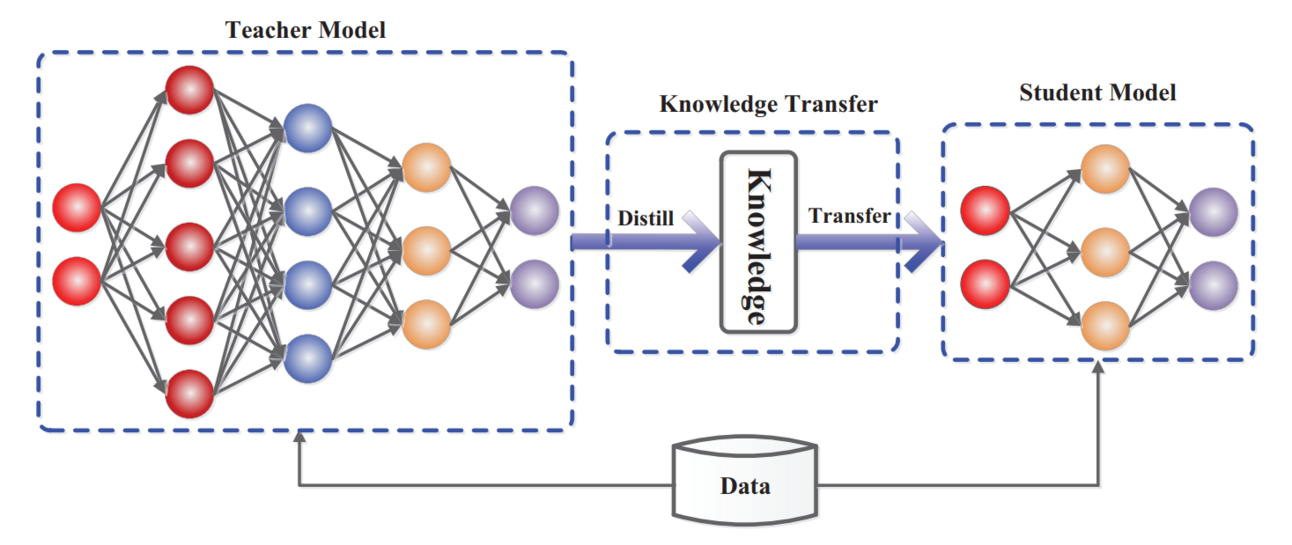
\includegraphics[width=0.8\textwidth]{knowledge_distillation.png}
    \captionof{figure}{Quy trình Chưng cất Tri thức. Mô hình trò học đồng thời từ nhãn cứng của dữ liệu và nhãn mềm (được tạo ra bởi mô hình thầy với nhiệt độ T).}
    \label{fig:knowledge_distillation}
\end{center}

Các mô hình như DistilBERT đã sử dụng kỹ thuật này để tạo ra một phiên bản BERT nhỏ hơn 40% và nhanh hơn 60% trong khi vẫn giữ lại 97% hiệu năng.

\subsection{Lượng tử hóa (Quantization)}
\label{ssec:quantization}

\subsubsection{Trực giác cốt lõi: Giảm độ chính xác của Số}
Lượng tử hóa là quá trình giảm số lượng bit được sử dụng để biểu diễn một con số. Trong học sâu, các trọng số và giá trị kích hoạt của mô hình thường được lưu trữ dưới dạng số thực dấu phẩy động 32-bit (FP32) hoặc 16-bit (FP16). Lượng tử hóa sẽ ánh xạ các giá trị này sang các định dạng có độ chính xác thấp hơn, ví dụ như số nguyên 8-bit (INT8) hoặc thậm chí 4-bit.

\begin{tcolorbox}[
    title=Triết lý của Lượng tử hóa,
    colback=blue!5!white, colframe=blue!75!black, fonttitle=\bfseries
]
"Chúng ta có thực sự cần đến 32 bit độ chính xác để lưu trữ mỗi trọng số không? Liệu việc làm tròn các trọng số thành một tập hợp các giá trị rời rạc, có độ chính xác thấp hơn có làm ảnh hưởng nhiều đến hiệu năng cuối cùng không?"
\end{tcolorbox}
Câu trả lời, một cách đáng ngạc nhiên, thường là "không nhiều". Các mạng nơ-ron sâu có một sự dư thừa (redundancy) nhất định và có khả năng chống chịu khá tốt với nhiễu và sự mất mát độ chính xác.

\subsubsection{Các phương pháp Lượng tử hóa}
\paragraph{Post-Training Quantization (PTQ) - Lượng tử hóa sau Huấn luyện}
Đây là phương pháp đơn giản nhất.
\begin{enumerate}
    \item Lấy một mô hình đã được huấn luyện đầy đủ.
    \item Chuyển đổi các trọng số của nó từ FP32/FP16 sang INT8. Quá trình này bao gồm việc tìm ra một "tỷ lệ" (scale) và một "điểm không" (zero-point) để ánh xạ khoảng giá trị thực sang khoảng giá trị nguyên 8-bit.
    \item Thường yêu cầu một bộ dữ liệu hiệu chỉnh nhỏ (calibration dataset) để tìm ra các tham số ánh xạ tối ưu.
\end{enumerate}
PTQ rất nhanh để thực hiện nhưng có thể gây ra sụt giảm độ chính xác đáng kể.

\paragraph{Quantization-Aware Training (QAT) - Huấn luyện Nhận biết Lượng tử hóa}
Đây là phương pháp phức tạp nhưng cho kết quả tốt hơn.
\begin{enumerate}
    \item Trong quá trình fine-tuning (hoặc huấn luyện từ đầu), mô hình sẽ \textbf{mô phỏng (simulate)} ảnh hưởng của việc lượng tử hóa.
    \item Tức là, trong quá trình truyền thẳng, các trọng số sẽ được "làm tròn" (quantized) về định dạng có độ chính xác thấp, nhưng trong quá trình truyền ngược, gradient vẫn được tính toán và cập nhật trên các trọng số có độ chính xác đầy đủ.
    \item Điều này cho phép mô hình học cách "thích ứng" với sự mất mát độ chính xác sẽ xảy ra sau khi lượng tử hóa, giúp giảm thiểu sụt giảm hiệu năng.
\end{enumerate}

Lợi ích của Lượng tử hóa là rất rõ ràng: giảm kích thước mô hình (INT8 nhỏ hơn FP32 4 lần) và tăng tốc độ suy luận (các phép toán trên số nguyên nhanh hơn nhiều so với số thực trên hầu hết các phần cứng). Chúng ta đã thấy một ứng dụng của nó trong QLoRA (mục \ref{ssec:qlora}).

\subsection{Cắt tỉa (Pruning)}
\label{ssec:pruning}

\subsubsection{Trực giác cốt lõi: Loại bỏ các Kết nối Thừa}
Các mạng nơ-ron lớn thường được "tham số hóa quá mức" (over-parameterized), nghĩa là chúng có nhiều trọng số và nơ-ron hơn mức cần thiết. Cắt tỉa là quá trình xác định và loại bỏ các trọng số hoặc các nơ-ron "ít quan trọng" nhất trong mạng.

\begin{tcolorbox}[
    title=Triết lý của Cắt tỉa,
    colback=red!5!white, colframe=red!75!black, fonttitle=\bfseries
]
"Một mạng nơ-ron giống như một cái cây. Sau khi nó phát triển, chúng ta có thể cắt tỉa đi những cành lá không cần thiết mà không làm ảnh hưởng đến sức sống và khả năng ra quả của cây, thậm chí còn giúp cây khỏe mạnh hơn."
\end{tcolorbox}

\subsubsection{Các phương pháp Cắt tỉa}
\paragraph{Cắt tỉa theo Độ lớn (Magnitude Pruning)}
Đây là phương pháp phổ biến nhất.
\begin{itemize}
    \item \textbf{Giả định:} Các trọng số có giá trị tuyệt đối gần bằng 0 là ít quan trọng nhất.
    \item \textbf{Quy trình:}
        \begin{enumerate}
            \item Huấn luyện một mô hình dày đặc đến khi hội tụ.
            \item Xóa (đặt bằng 0) tất cả các trọng số có giá trị tuyệt đối nhỏ hơn một ngưỡng nhất định. Điều này tạo ra một ma trận trọng số "thưa thớt" (sparse).
            \item (Tùy chọn nhưng quan trọng) Fine-tune lại mô hình thưa thớt này trong một vài epoch để cho phép các trọng số còn lại "bù đắp" cho các trọng số đã bị xóa.
        \end{enumerate}
\end{itemize}

\paragraph{Cắt tỉa có Cấu trúc vs. Không có Cấu trúc (Structured vs. Unstructured Pruning)}
\begin{itemize}
    \item \textbf{Không có cấu trúc:} Xóa các trọng số riêng lẻ ở bất kỳ đâu trong ma trận. Điều này tạo ra các ma trận thưa thớt, có thể giảm đáng kể số lượng tham số nhưng không phải lúc nào cũng tăng tốc độ trên phần cứng thông thường (như GPU) vốn được tối ưu cho các phép toán ma trận dày đặc.
    \item \textbf{Có cấu trúc:} Xóa toàn bộ các cấu trúc lớn hơn, ví dụ như xóa toàn bộ một nơ-ron (một cột trong ma trận trọng số) hoặc toàn bộ một bộ lọc trong CNN. Phương pháp này có thể không giảm được nhiều tham số bằng, nhưng kết quả là một mô hình nhỏ hơn, dày đặc hơn, có thể chạy nhanh hơn trên phần cứng hiện có mà không cần các thư viện đặc biệt.
\end{itemize}

\begin{center}
    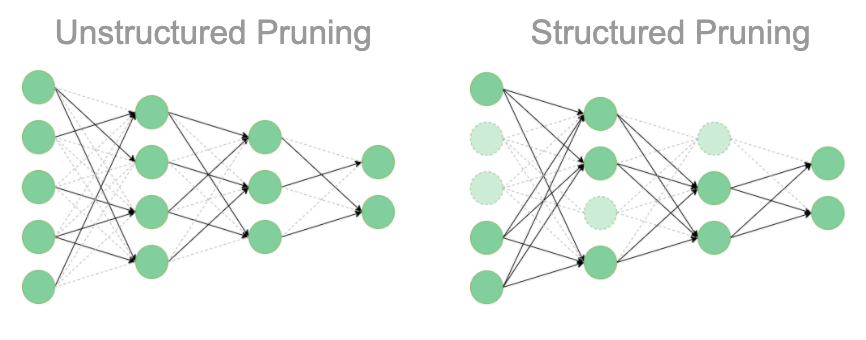
\includegraphics[width=1.0\textwidth]{pruning_types.png}
    \captionof{figure}{So sánh Cắt tỉa Không có Cấu trúc (xóa các trọng số riêng lẻ, tạo ma trận thưa thớt) và Cắt tỉa Có Cấu trúc (xóa toàn bộ cột/nơ-ron, tạo ma trận nhỏ hơn).}
    \label{fig:pruning_types}
\end{center}

Các kỹ thuật tối ưu hóa này thường được sử dụng kết hợp với nhau (ví dụ, một mô hình được chưng cất, sau đó được cắt tỉa và cuối cùng được lượng tử hóa) để đạt được sự cân bằng tốt nhất giữa kích thước, tốc độ và độ chính xác.
% % !TEX root = ../main.tex
% File: chapters_part1/chap6_3.tex
% Nội dung cho Chương 6, Phần 3

\section{Mô hình Đa phương thức (Multimodal Models)}
\label{sec:multimodal_models}

Con người trải nghiệm thế giới thông qua nhiều giác quan cùng một lúc: chúng ta nhìn thấy một hình ảnh, nghe một âm thanh, và đọc một đoạn văn bản mô tả về nó. Các mô hình mà chúng ta đã thảo luận cho đến nay chủ yếu là đơn phương thức (unimodal) - chúng chỉ xử lý văn bản. Để AI thực sự tiến gần hơn đến trí thông minh của con người, chúng cần có khả năng hiểu và lý luận trên nhiều loại dữ liệu khác nhau một cách đồng thời. Đây chính là mục tiêu của các \textbf{Mô hình Đa phương thức (Multimodal Models)}.

Lĩnh vực này đã có những bước nhảy vọt phi thường, đặc biệt là trong việc kết hợp hai phương thức quan trọng nhất: \textbf{Ngôn ngữ (Language)} và \textbf{Thị giác (Vision)}. Phần này sẽ đi sâu vào các kiến trúc nền tảng đã tạo nên cuộc cách mạng này.

\subsection{Nền tảng: Xây dựng cầu nối giữa Ảnh và Chữ}
\label{ssec:multimodal_foundations}

Để một mô hình có thể hiểu cả ảnh và chữ, nó cần một "ngôn ngữ chung" - một không gian biểu diễn nơi cả ảnh và chữ đều có thể được ánh xạ vào và so sánh với nhau. Hai đột phá nền tảng đã tạo ra cây cầu này là Vision Transformer (ViT) và Contrastive Learning (CLIP).

\subsubsection{Vision Transformer (ViT): "Đọc" ảnh như đọc một câu}
\paragraph{Vấn đề với CNN}
Các mạng CNN (đã học ở mục \ref{sec:cnn_for_nlp}) xử lý ảnh bằng cách trượt các bộ lọc nhỏ, xây dựng các đặc trưng từ cục bộ (cạnh, góc) đến toàn cục (mắt, mũi, khuôn mặt). Cách tiếp cận này rất hiệu quả nhưng lại có một sự khác biệt về kiến trúc so với Transformer đang thống trị NLP.

\paragraph{Giải pháp của ViT: Biến ảnh thành một chuỗi các "từ"}
Vision Transformer (Dosovitskiy et al., 2020) đã đưa ra một ý tưởng cấp tiến:
\begin{tcolorbox}[
    title=Trực giác của Vision Transformer,
    colback=blue!5!white, colframe=blue!75!black, fonttitle=\bfseries
]
"Điều gì sẽ xảy ra nếu chúng ta coi một bức ảnh không phải là một lưới pixel, mà là một \textbf{chuỗi các mảnh vá (sequence of patches)}? Nếu vậy, chúng ta có thể đưa chuỗi các mảnh vá này vào một kiến trúc Transformer tiêu chuẩn, giống hệt như cách chúng ta xử lý một chuỗi các từ."
\end{tcolorbox}

\paragraph{Cơ chế hoạt động}
\begin{enumerate}
    \item \textbf{Phân mảnh Ảnh (Image Patching):} Một bức ảnh đầu vào (ví dụ: $224 \times 224$ pixel) được chia thành một lưới các mảnh vá không chồng chéo có kích thước cố định (ví dụ: $16 \times 16$ pixel). Điều này tạo ra một chuỗi gồm $(224/16)^2 = 14 \times 14 = 196$ mảnh vá.
    \item \textbf{Nhúng Mảnh vá (Patch Embedding):} Mỗi mảnh vá được "làm phẳng" (flatten) thành một vector dài và sau đó được chiếu qua một lớp tuyến tính để tạo ra một "patch embedding" có số chiều phù hợp với Transformer (ví dụ: 768 chiều).
    \item \textbf{Thêm Token Phân loại và Mã hóa Vị trí:} Tương tự như BERT, một token `[CLS]` có thể học được sẽ được chèn vào đầu chuỗi. Sau đó, các vector mã hóa vị trí (positional encodings) được cộng vào mỗi patch embedding để cung cấp thông tin về vị trí tương đối của các mảnh vá.
    \item \textbf{Đưa vào Transformer Encoder:} Chuỗi các patch embedding này giờ đây được xử lý bởi một chuỗi các khối Transformer Encoder tiêu chuẩn. Cơ chế Self-Attention sẽ cho phép mỗi mảnh vá "chú ý" đến tất cả các mảnh vá khác để học các mối quan hệ không gian.
\end{enumerate}

\begin{center}
    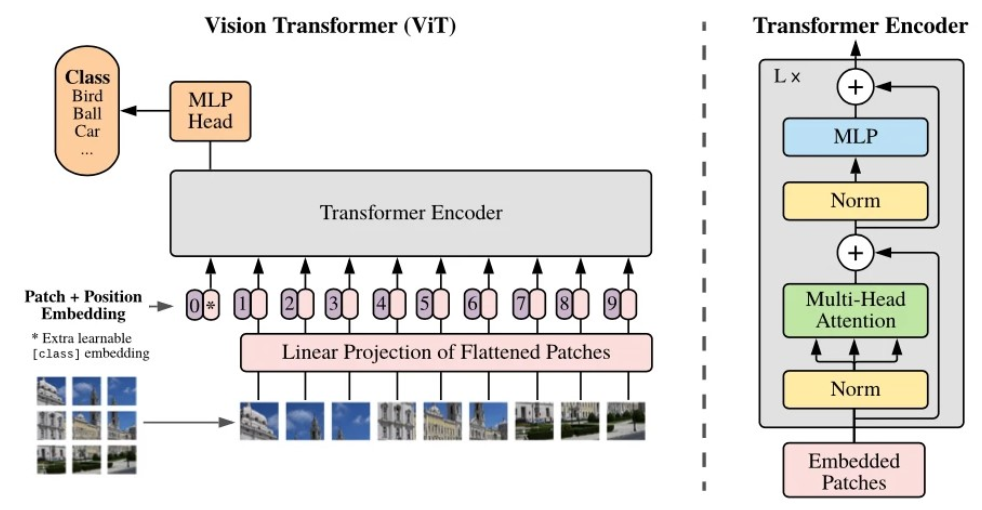
\includegraphics[width=1.0\textwidth]{vision_transformer_vit.png}
    \captionof{figure}{Kiến trúc của Vision Transformer (ViT). Ảnh được chia thành các mảnh vá, mỗi mảnh được nhúng và xử lý như một "token" trong một chuỗi bởi một Transformer Encoder tiêu chuẩn.}
    \label{fig:vision_transformer_vit}
\end{center}

ViT đã chứng minh rằng một kiến trúc dựa hoàn toàn trên Transformer có thể đạt được hiệu năng state-of-the-art trong các tác vụ thị giác, tạo ra một sự thống nhất về mặt kiến trúc giữa NLP và CV. Nó cung cấp một cách mạnh mẽ để có được các \textbf{bộ mã hóa hình ảnh (Image Encoders)} tạo ra các biểu diễn giàu ngữ cảnh cho ảnh.

\subsubsection{CLIP: Học sự tương đồng giữa Ảnh và Chữ bằng Contrastive Learning}
\paragraph{Vấn đề}
Chúng ta đã có Image Encoder (ViT) và Text Encoder (Transformer). Làm thế nào để chúng "nói chuyện" với nhau? Làm thế nào để mô hình biết rằng bức ảnh một chú chó và câu "a photo of a dog" là cùng một khái niệm?

\paragraph{Giải pháp của CLIP (Contrastive Language-Image Pre-training)}
CLIP (Radford et al., 2021) từ OpenAI đã giải quyết vấn đề này bằng một phương pháp huấn luyện quy mô lớn dựa trên \textbf{Học Tương phản (Contrastive Learning)}, một ý tưởng tương tự như Mạng Siamese (mục \ref{sec:siamese_networks}).

\paragraph{Cơ chế hoạt động}
\begin{enumerate}
    \item \textbf{Kiến trúc:} CLIP bao gồm hai bộ mã hóa riêng biệt:
        \begin{itemize}
            \item Một \textbf{Image Encoder} (ví dụ: ViT).
            \item Một \textbf{Text Encoder} (ví dụ: một Transformer).
        \end{itemize}
    \item \textbf{Dữ liệu Huấn luyện:} Một bộ dữ liệu khổng lồ gồm 400 triệu cặp \textbf{(ảnh, văn bản mô tả)} được thu thập từ Internet.
    \item \textbf{Mục tiêu Huấn luyện:} Huấn luyện cả hai bộ mã hóa từ đầu để chúng ánh xạ các cặp (ảnh, văn bản) tương ứng vào \textbf{cùng một vị trí} trong một không gian embedding đa phương thức chung.
    \item \textbf{Quy trình trong một batch:}
        \begin{enumerate}
            \item Lấy một batch gồm $N$ cặp (ảnh, văn bản).
            \item Đưa $N$ ảnh qua Image Encoder để có được $N$ vector ảnh ($I_1, \dots, I_N$).
            \item Đưa $N$ văn bản qua Text Encoder để có được $N$ vector văn bản ($T_1, \dots, T_N$).
            \item Tính toán độ tương đồng cosine giữa \textbf{tất cả} các cặp vector ảnh và văn bản có thể có, tạo ra một ma trận tương đồng $N \times N$.
            \item \textbf{Hàm mất mát tương phản:} Mục tiêu là làm cho độ tương đồng của các cặp \textbf{khớp đúng} (ví dụ: $I_i$ và $T_i$) trên đường chéo chính của ma trận là cao nhất, và độ tương đồng của tất cả các cặp \textbf{không khớp} ($I_i$ và $T_j$ với $i \neq j$) là thấp nhất.
        \end{enumerate}
\end{enumerate}

\begin{center}
    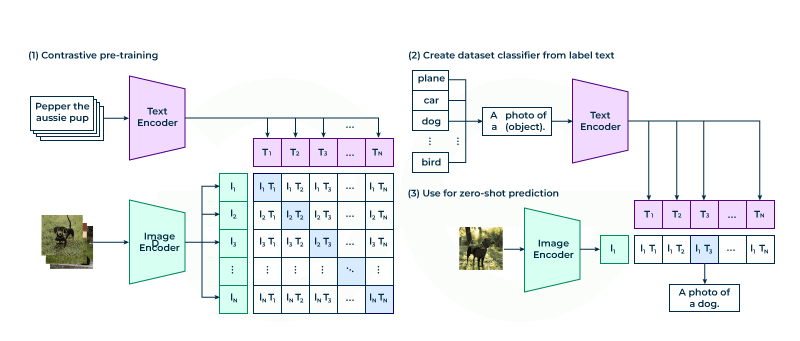
\includegraphics[width=1.0\textwidth]{clip_contrastive_learning.png}
    \captionof{figure}{Quy trình huấn luyện của CLIP. Mô hình học cách tối đa hóa độ tương đồng của các cặp (ảnh, văn bản) chính xác trên đường chéo chính và tối thiểu hóa độ tương đồng của các cặp không chính xác.}
    \label{fig:clip_contrastive_learning}
\end{center}

Sau khi huấn luyện, CLIP có khả năng zero-shot đáng kinh ngạc trong việc phân loại ảnh. Ví dụ, để phân loại một ảnh, bạn chỉ cần nhúng ảnh đó và so sánh độ tương đồng của nó với các vector văn bản được tạo từ các prompt như "a photo of a dog", "a photo of a cat",... và chọn prompt có độ tương đồng cao nhất.

Quan trọng hơn, CLIP đã tạo ra một \textbf{không gian embedding đa phương thức được căn chỉnh (aligned multimodal embedding space)} mạnh mẽ, là nền tảng cho các mô hình thế hệ tiếp theo.

\subsection{Ví dụ Kiến trúc: Kết hợp LLM với Thị giác}
\label{ssec:multimodal_architectures_examples}
Với các khối xây dựng là Image Encoder và không gian đa phương thức được căn chỉnh, các nhà nghiên cứu đã tạo ra các Mô hình Ngôn ngữ Lớn Đa phương thức (Multimodal Large Language Models - MLLMs).

\subsubsection{Flamingo: Thêm Cross-Attention vào một LLM đã đóng băng}
\begin{itemize}
    \item \textbf{Kiến trúc (Alayrac et al., 2022):} Flamingo giữ một LLM văn bản (ví dụ: Chinchilla) và một Vision Encoder (ví dụ: ViT) đã được huấn luyện trước và \textbf{đóng băng (frozen)} chúng.
    \item \textbf{Cơ chế kết nối:} Nó chèn các lớp \textbf{Cross-Attention} đặc biệt vào giữa các lớp của LLM.
    \item \textbf{Dòng chảy dữ liệu:} Khi xử lý văn bản, các token văn bản sẽ đi qua các lớp Transformer của LLM như bình thường. Tại các lớp Cross-Attention, các token văn bản này sẽ đóng vai trò là \textbf{Query}, trong khi các đặc trưng hình ảnh từ Vision Encoder sẽ đóng vai trò là \textbf{Key} và \textbf{Value}. Điều này cho phép các token văn bản "nhìn" vào hình ảnh và rút ra các thông tin thị giác liên quan khi cần thiết.
    \item \textbf{Lợi ích:} Rất hiệu quả về mặt tham số vì chỉ cần huấn luyện các lớp Cross-Attention mới.
\end{itemize}

\subsubsection{LLaVA: Ánh xạ Trực tiếp vào Không gian Từ của LLM}
LLaVA (Large Language and Vision Assistant - Liu et al., 2023) đưa ra một cách tiếp cận đơn giản hơn nhưng lại cực kỳ hiệu quả.
\begin{itemize}
    \item \textbf{Kiến trúc:} Sử dụng một Vision Encoder (cụ thể là ViT từ CLIP) và một LLM (cụ thể là Vicuna, một phiên bản của Llama).
    \item \textbf{Cơ chế kết nối:}
        \begin{enumerate}
            \item Ảnh được đưa qua Vision Encoder để tạo ra một chuỗi các patch embedding.
            \item Một \textbf{lớp chiếu tuyến tính (projection layer)} nhỏ duy nhất được huấn luyện để \textbf{ánh xạ (map)} các patch embedding này vào cùng một không gian với các word embedding của LLM.
            \item Các patch embedding đã được chiếu này sau đó được coi như các "từ" đặc biệt và được \textbf{chèn trực tiếp} vào chuỗi văn bản đầu vào của LLM.
        \end{enumerate}
    \item \textbf{Quá trình huấn luyện 2 giai đoạn:}
        \begin{enumerate}
            \item \textbf{Giai đoạn 1 (Căn chỉnh đặc trưng):} Đóng băng cả Vision Encoder và LLM, chỉ huấn luyện lớp chiếu tuyến tính trên một bộ dữ liệu lớn gồm các cặp (ảnh, mô tả). Giai đoạn này dạy cho lớp chiếu cách "dịch" đặc trưng ảnh thành "ngôn ngữ" mà LLM có thể hiểu.
            \item \textbf{Giai đoạn 2 (Tinh chỉnh End-to-End):} Mở đóng băng các trọng số của LLM và fine-tune toàn bộ mô hình (hoặc chỉ lớp chiếu và LLM) trên một bộ dữ liệu nhỏ hơn, chất lượng cao hơn gồm các chỉ dẫn đa phương thức phức tạp (ví dụ: các cuộc trò chuyện về hình ảnh).
        \end{enumerate}
    \item \textbf{Lợi ích:} Kiến trúc cực kỳ đơn giản, dễ triển khai và tận dụng được sức mạnh của các LLM và Vision Encoder đã có sẵn. LLaVA đã trở thành một trong những kiến trúc nền tảng cho các MLLM mã nguồn mở.
\end{itemize}

Sự kết hợp giữa Ngôn ngữ và Thị giác đang mở ra một kỷ nguyên mới của AI, nơi các mô hình có thể tương tác với thế giới một cách phong phú và tự nhiên hơn rất nhiều.

\subsection{Sinh Đa phương thức (Multimodal Generation)}
\label{ssec:multimodal_generation}

Nếu các mô hình ở mục trước tập trung vào việc \textit{hiểu} đầu vào đa phương thức (ví dụ, mô tả một bức ảnh bằng văn bản), thì một trong những bước đột phá ngoạn mục nhất của AI hiện đại là khả năng \textit{sinh} ra một phương thức từ một phương thức khác. Nổi bật nhất trong số đó là các tác vụ sinh từ văn bản, biến những mô tả trừu tượng thành các sản phẩm thị giác cụ thể.

\subsubsection{Sinh Ảnh từ Văn bản (Text-to-Image)}
Đây là lĩnh vực đã tạo ra một cuộc cách mạng trong ngành công nghiệp sáng tạo, cho phép bất kỳ ai cũng có thể tạo ra các tác phẩm nghệ thuật kỹ thuật số chỉ bằng ngôn ngữ.
\begin{itemize}
    \item \textbf{Bài toán:} Cho một câu mô tả bằng văn bản (prompt), ví dụ "một phi hành gia đang cưỡi ngựa trên sao Hỏa theo phong cách siêu thực", mô hình phải tạo ra một bức ảnh hoàn toàn mới khớp với mô tả đó.
    \item \textbf{Kiến trúc cốt lõi: Mô hình Khuếch tán (Diffusion Models)} Các mô hình thành công nhất hiện nay như DALL-E 2, Midjourney, và Stable Diffusion thường dựa trên kiến trúc này.
        \begin{enumerate}
            \item \textbf{Mã hóa Văn bản:} Prompt được đưa qua một bộ mã hóa văn bản mạnh mẽ (thường là một phần của mô hình CLIP) để tạo ra một vector embedding giàu ngữ nghĩa.
            \item \textbf{Quá trình Khuếch tán Ngược có Điều kiện:} Mô hình bắt đầu với một bức ảnh chỉ toàn nhiễu ngẫu nhiên (random noise). Sau đó, trong một chuỗi nhiều bước, một mạng nơ-ron (thường là U-Net) sẽ dần dần \textbf{khử nhiễu (denoise)} cho bức ảnh. Ở mỗi bước, quá trình khử nhiễu này được \textit{dẫn dắt} (conditioned) bởi vector embedding của văn bản. Quá trình này dần dần làm hiện ra một hình ảnh mạch lạc và khớp với prompt.
        \end{enumerate}
\end{itemize}
\begin{center}
    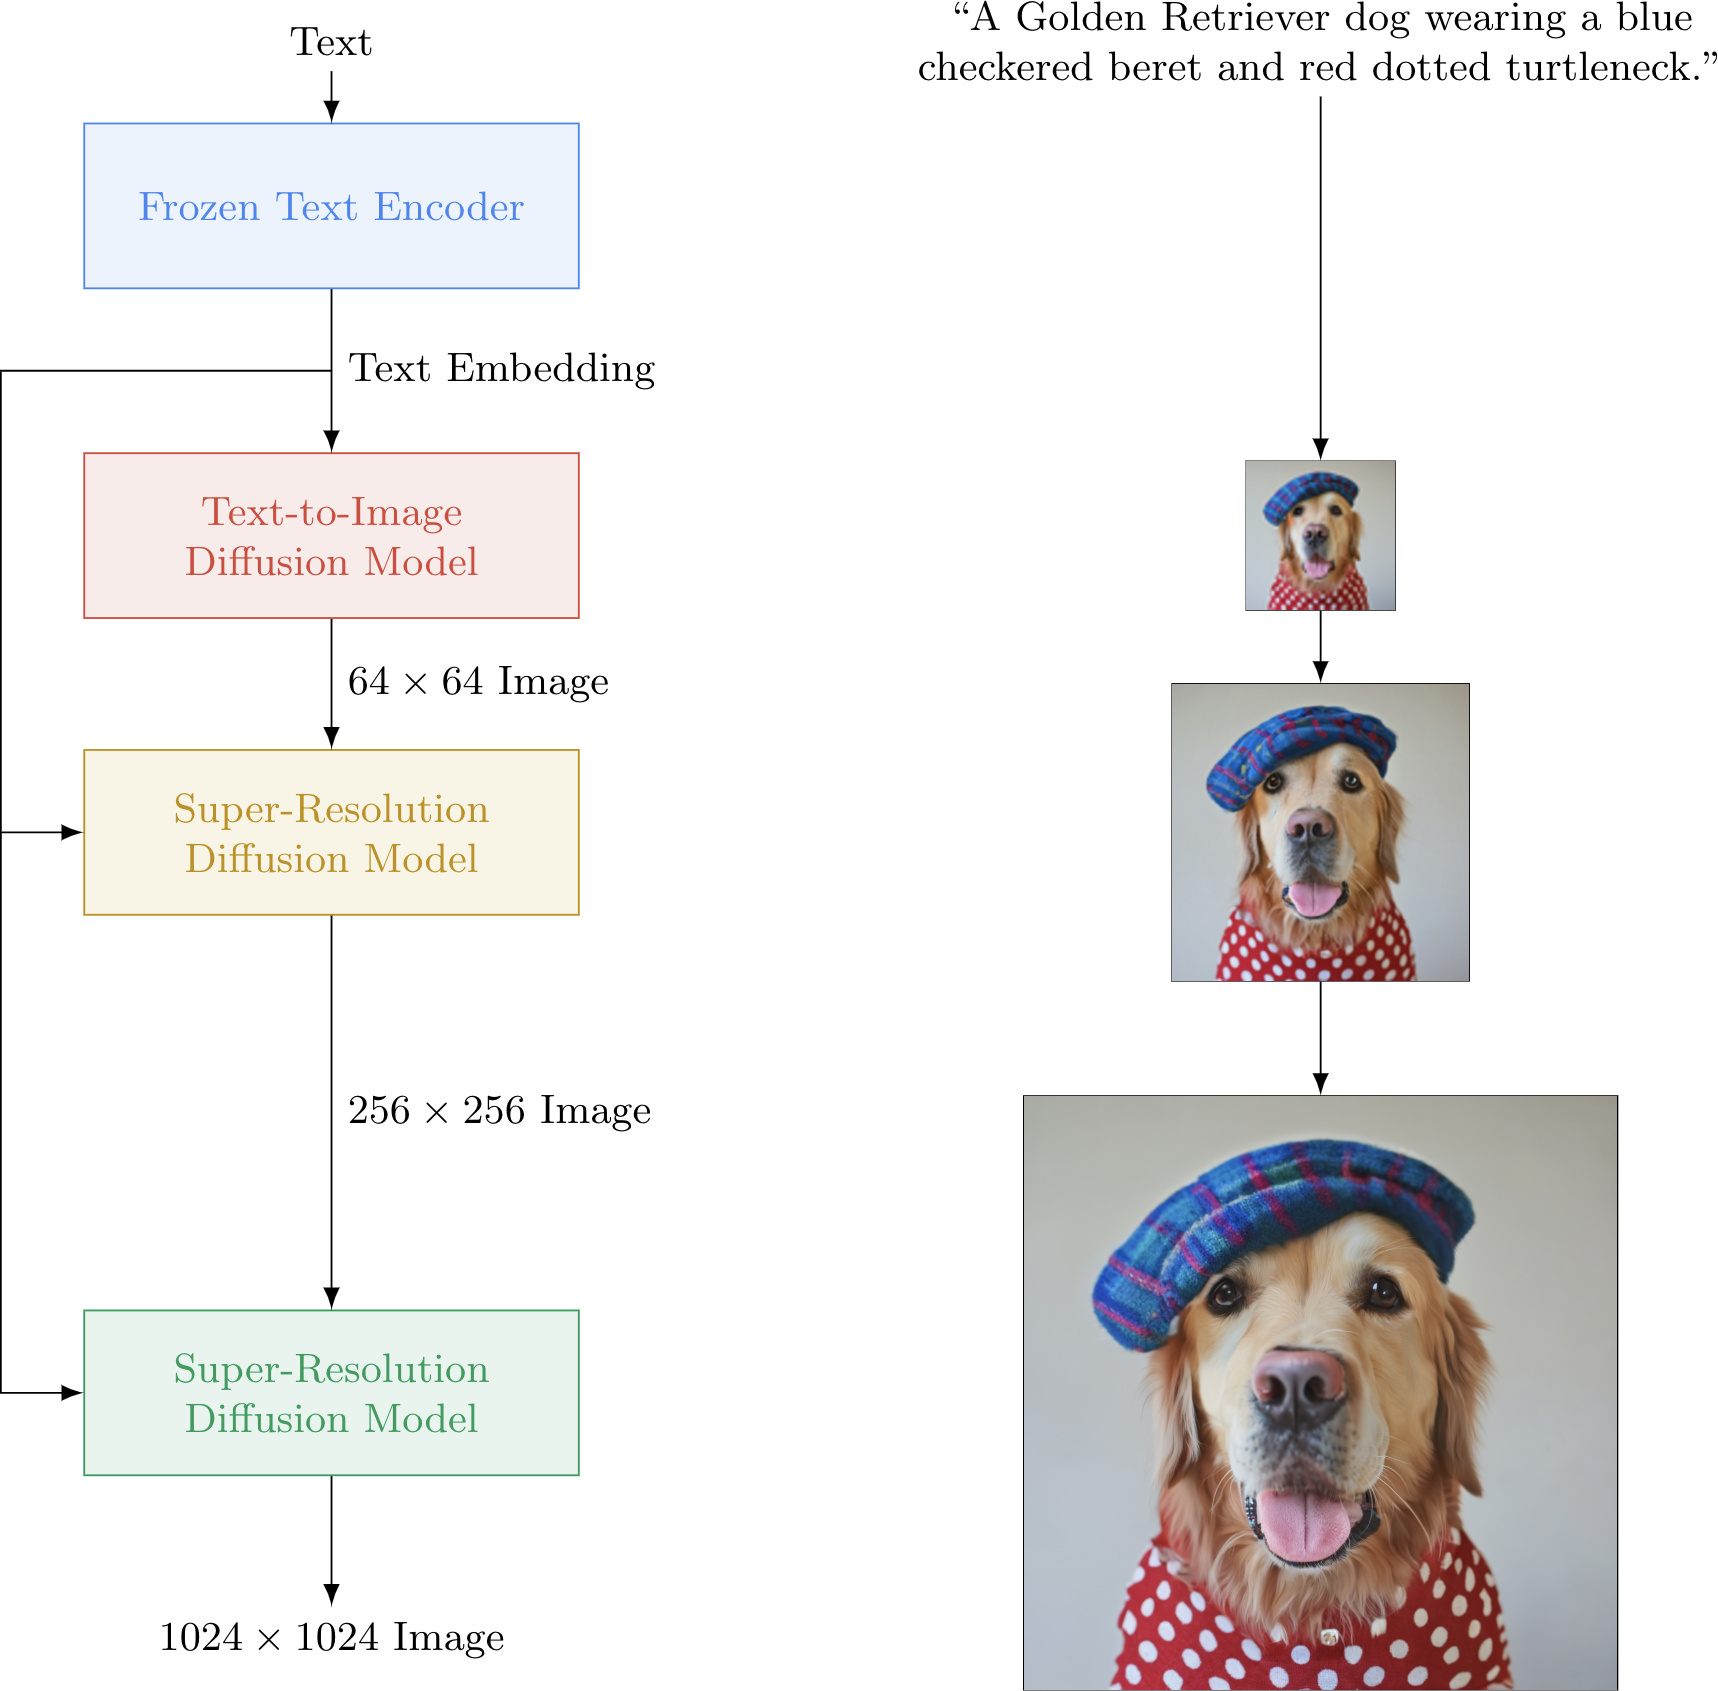
\includegraphics[width=1.0\textwidth]{text_to_image_diffusion.jpg}
    \captionof{figure}{Mô hình Khuếch tán cho việc sinh ảnh từ văn bản. Bắt đầu từ nhiễu, mô hình dần dần khử nhiễu theo sự dẫn dắt của embedding văn bản để tạo ra ảnh cuối cùng.}
    \label{fig:text_to_image_diffusion}
\end{center}

\subsubsection{Sinh Video từ Văn bản (Text-to-Video)}
Là một bước tiến tự nhiên nhưng khó hơn rất nhiều so với sinh ảnh.
\begin{itemize}
    \item \textbf{Thách thức chính:} Ngoài việc tạo ra các khung hình (frames) chất lượng cao, mô hình còn phải đảm bảo \textbf{tính nhất quán về mặt thời gian (temporal consistency)}. Các đối tượng và bối cảnh phải duy trì sự logic và liền mạch từ khung hình này sang khung hình tiếp theo.
    \item \textbf{Hướng tiếp cận:} Các mô hình tiên tiến như Sora (OpenAI) hay Lumiere (Google) mở rộng ý tưởng của mô hình khuếch tán sang không-thời gian. Chúng không xử lý từng khung hình riêng lẻ mà xử lý một loạt các khung hình hoặc toàn bộ "patch" không-thời gian cùng lúc để đảm bảo sự mượt mà và nhất quán của chuyển động và bối cảnh.
\end{itemize}

Việc làm chủ khả năng sinh đa phương thức không chỉ mở ra những ứng dụng sáng tạo mới mà còn là một bước tiến quan trọng hướng tới các hệ thống AI có khả năng tương tác và sáng tạo trong một thế giới đa dạng về phương thức như thế giới của chúng ta.

\subsection{Kiểm soát Quá trình Sinh (Controlled Generation)}
\label{ssec:controlled_generation}

Trong nhiều ứng dụng thực tế, yêu cầu không chỉ dừng lại ở việc sinh văn bản mạch lạc và tự nhiên, mà còn phải đảm bảo \textbf{tuân theo các ràng buộc} (constraints) hoặc \textbf{thuộc tính} (attributes) cụ thể. Ví dụ:
\begin{itemize}
    \item Sinh bài đánh giá sản phẩm với \textit{sentiment} tích cực.
    \item Viết tóm tắt nhưng \textbf{giữ nguyên thuật ngữ chuyên ngành}.
    \item Sinh hội thoại chatbot với \textbf{giọng điệu thân thiện}.
\end{itemize}

Đây là bài toán về việc ``\textbf{lái}'' quá trình sinh ngôn ngữ của LLM theo mong muốn của người dùng hoặc hệ thống.

\subsubsection{Các kỹ thuật kinh điển}
\label{sssec:classic_controlled_generation}

\paragraph{CTRL (Conditional Transformer Language Model)}
\begin{itemize}
    \item Ý tưởng: thêm các \textbf{mã kiểm soát (control codes)} đặc biệt vào đầu prompt để chỉ định thuộc tính mong muốn. 
    \item Ví dụ: \texttt{Reviews Rating: 5.0 The product was ...} để mô hình sinh tiếp một đánh giá tích cực.
    \item Ưu điểm: đơn giản, trực quan.
    \item Nhược điểm: đòi hỏi mô hình được \textbf{huấn luyện lại từ đầu} với dữ liệu gắn kèm mã kiểm soát; khó áp dụng cho nhiều thuộc tính phức tạp.
\end{itemize}

\paragraph{PPLM (Plug and Play Language Models)}
\begin{itemize}
    \item Ý tưởng: sử dụng một \textbf{mô hình thuộc tính nhỏ} (ví dụ: bộ phân loại cảm xúc) để hướng dẫn LLM đã đóng băng. 
    \item Cách làm: tại mỗi bước sinh, gradient từ mô hình thuộc tính sẽ \textbf{điều chỉnh trạng thái ẩn} của LLM để tăng xác suất sinh ra từ phù hợp.
    \item Ưu điểm: không cần huấn luyện lại LLM lớn; dễ áp dụng cho nhiều thuộc tính.
    \item Nhược điểm: chi phí tính toán cao do phải tính gradient trong lúc sinh; có thể làm giảm độ mạch lạc.
\end{itemize}

\paragraph{FUDGE (Future Discriminators for Generation)}
\begin{itemize}
    \item Thay vì chỉnh trực tiếp trạng thái ẩn, FUDGE huấn luyện một bộ phân loại để ước lượng \textbf{khả năng tiếp diễn thoả mãn thuộc tính}, sau đó kết hợp với xác suất sinh từ mô hình chính.
    \item Ưu điểm: linh hoạt, không cần huấn luyện lại LLM lớn.
    \item Nhược điểm: vẫn bị trade-off giữa kiểm soát và chất lượng.
\end{itemize}

\subsubsection{Các kỹ thuật dựa trên Prompt}
\label{sssec:prompt_based_controlled_generation}

Các phương pháp này thuộc nhóm \textbf{PEFT (Parameter-Efficient Fine-Tuning)} và hiện được ứng dụng rộng rãi do hiệu quả cao.

\paragraph{Prompt Tuning}
\begin{itemize}
    \item Học các \textbf{prompt mềm (soft prompts)} — tức là các vector embedding có thể học được — để hướng dẫn mô hình.
    \item Ví dụ: để điều khiển văn bản theo giọng điệu ``lịch sự'', ta học một soft prompt tương ứng và nối nó vào trước input.
    \item Ưu điểm: nhẹ, không cần tinh chỉnh toàn bộ mô hình.
    \item Nhược điểm: hiệu quả hạn chế nếu số lượng thuộc tính cần kiểm soát quá nhiều.
\end{itemize}

\paragraph{Prefix Tuning}
\begin{itemize}
    \item Ý tưởng: học các vector embedding ``tiền tố'' và \textbf{chèn vào mỗi lớp Transformer}.
    \item Nhờ vậy, prompt không chỉ ảnh hưởng ở input mà còn tác động trực tiếp lên \textbf{attention} của mọi tầng.
    \item Hiệu quả hơn Prompt Tuning trong nhiều tác vụ yêu cầu kiểm soát tinh vi.
\end{itemize}

\paragraph{LoRA (Low-Rank Adaptation) và Adapter Tuning}
\begin{itemize}
    \item LoRA chèn thêm ma trận hạng thấp vào trong trọng số attention, trong khi Adapter Tuning chèn ``mô-đun phụ'' vào giữa các lớp Transformer.
    \item Cả hai cho phép học thêm một số ít tham số để kiểm soát phong cách, giọng điệu hoặc thuộc tính sinh.
\end{itemize}

\paragraph{In-Context Control}
\begin{itemize}
    \item Không cần tinh chỉnh mô hình, chỉ cần đưa \textbf{ví dụ minh hoạ (few-shot)} vào prompt.
    \item Ví dụ: nếu muốn mô hình sinh phản hồi ngắn gọn, ta có thể thêm vào prompt vài ví dụ ``câu trả lời ngắn''.
    \item Đây là phương pháp thực tế nhất trong triển khai API, tuy nhiên không ổn định khi yêu cầu phức tạp.
\end{itemize}

\subsubsection{Các hướng mở rộng hiện đại}
\begin{itemize}
    \item \textbf{RLHF (Reinforcement Learning from Human Feedback)}: dùng con người để đánh giá và tinh chỉnh chính sách sinh, giúp mô hình tuân theo các chuẩn mực xã hội.
    \item \textbf{Direct Preference Optimization (DPO)}: thay thế RLHF truyền thống bằng tối ưu trực tiếp trên dữ liệu so sánh, đơn giản hơn.
    \item \textbf{Control bằng ràng buộc hình thức}: ví dụ đảm bảo output phải là JSON hợp lệ, hoặc đảm bảo không vi phạm regex.
    \item \textbf{Multi-attribute control}: điều khiển đồng thời nhiều thuộc tính (ví dụ: văn bản vừa ``tích cực'' vừa ``ngắn gọn'').
\end{itemize}

\subsection{Sinh Nhận biết Cấu trúc (Structure-aware Generation)}
\label{ssec:structure_aware_generation}

Một thách thức lớn khác là sinh ngôn ngữ tự nhiên từ dữ liệu có cấu trúc (\textit{structured data}) như \textbf{bảng}, \textbf{cơ sở dữ liệu}, hoặc \textbf{đồ thị tri thức}. Đây là nền tảng cho nhiều ứng dụng: báo cáo tự động, sinh mô tả sản phẩm, hoặc trợ lý ảo truy vấn dữ liệu.

\subsubsection{Sinh Văn bản từ Bảng (Table-to-text)}
\begin{itemize}
    \item \textbf{Bài toán:} Cho một bảng dữ liệu, sinh ra đoạn văn mô tả hoặc tóm tắt thông tin.
    \item \textbf{Hướng tiếp cận:}
    \begin{enumerate}
        \item \textbf{Tuyến tính hoá (linearization)}: biến bảng thành chuỗi 1D với các token đặc biệt cho hàng/cột/ô, rồi dùng Seq2Seq (T5, BART).
        \item \textbf{Schema-guided generation}: tận dụng nhãn cột/hàng để hướng dẫn mô hình.
        \item \textbf{Pretraining đặc thù}: ví dụ TAPAS (Google) huấn luyện trực tiếp trên bảng + câu hỏi.
    \end{enumerate}
\end{itemize}

\subsubsection{Sinh Văn bản từ Đồ thị (Graph-to-text)}
\begin{itemize}
    \item \textbf{Bài toán:} Cho một đồ thị tri thức (Knowledge Graph), sinh ra mô tả bằng ngôn ngữ tự nhiên.
    \item \textbf{Hướng tiếp cận:}
    \begin{enumerate}
        \item \textbf{Mạng nơ-ron đồ thị (GNN)} để mã hoá cấu trúc quan hệ thành embedding.
        \item Transformer \textbf{attend} lên embedding này để sinh chuỗi văn bản.
        \item Một số mô hình tiêu biểu: \textit{GraphWriter}, \textit{KG-to-Text}.
    \end{enumerate}
\end{itemize}

\subsubsection{Sinh Văn bản từ CSDL (Data-to-text)}
\begin{itemize}
    \item \textbf{Ví dụ:} Sinh báo cáo tài chính tự động từ số liệu.
    \item \textbf{Cách làm:} Tương tự table-to-text nhưng bổ sung thêm cơ chế \textbf{content planning} để quyết định thông tin nào cần nhắc đến trước.
\end{itemize}

% % !TEX root = ../main.tex
% File: chapters_part1/chap6_4.tex
% Nội dung cho Chương 6, Phần 4

\section{Hệ thống Tác tử (Agentic Systems) với LLMs}
\label{sec:agentic_systems}

Cho đến nay, chúng ta chủ yếu xem LLM như một bộ não xử lý thông tin và sinh ra văn bản. Nhưng điều gì sẽ xảy ra nếu chúng ta trao cho bộ não đó "tay chân" để tương tác với thế giới bên ngoài? Đây chính là ý tưởng đằng sau các \textbf{Hệ thống Tác tử (Agentic Systems)}.

Một Tác tử LLM (LLM Agent) không chỉ đơn thuần trả lời một câu hỏi. Nó là một hệ thống tự hành có khả năng:
\begin{itemize}
    \item \textbf{Phân rã (Decompose)} một mục tiêu phức tạp thành các bước nhỏ hơn.
    \item \textbf{Lập kế hoạch (Plan)} một chuỗi các hành động để thực hiện các bước đó.
    \item \textbf{Sử dụng công cụ (Use Tools)} như truy cập API, chạy mã nguồn, hoặc tìm kiếm trên web để thu thập thông tin và thực hiện hành động.
    \item \textbf{Quan sát (Observe)} kết quả của các hành động và \textbf{tự sửa lỗi (self-correct)} nếu cần.
\end{itemize}

Về cơ bản, chúng ta đang cố gắng xây dựng một vòng lặp, trong đó LLM đóng vai trò là "bộ não" ra quyết định, và các công cụ bên ngoài là "cơ thể" thực thi.

\subsection{Vòng lặp Suy luận-Hành động: Khung sườn ReAct}
\label{ssec:react_framework}

Một trong những khung sườn (frameworks) nền tảng và có ảnh hưởng nhất cho việc xây dựng Tác tử là \textbf{ReAct (Reasoning and Acting)} (Yao et al., 2022).

\begin{tcolorbox}[
    title=Triết lý của ReAct,
    colback=green!5!white, colframe=green!60!black, fonttitle=\bfseries
]
ReAct đề xuất rằng để hoàn thành một mục tiêu, một Tác tử nên xen kẽ một cách linh hoạt giữa hai hành vi nguyên thủy: \textbf{Suy luận (Reasoning)} và \textbf{Hành động (Acting)}. Việc suy luận giúp Tác tử xây dựng và điều chỉnh kế hoạch, trong khi việc hành động giúp nó thu thập thông tin mới từ môi trường bên ngoài để củng cố cho các suy luận tiếp theo.
\end{tcolorbox}

\subsubsection{Cơ chế hoạt động}
ReAct hoạt động bằng cách dạy cho LLM sinh ra các "lượt lời" có một định dạng đặc biệt, bao gồm:
\begin{enumerate}
    \item \textbf{Thought (Suy tưởng):} Một đoạn văn bản mô tả dòng suy nghĩ của Tác tử, phân tích tình hình hiện tại, và quyết định bước tiếp theo. Đây là phần suy luận.
    \item \textbf{Action (Hành động):} Một lệnh gọi đến một công cụ cụ thể. Ví dụ: `search[thủ đô của Pháp]` hoặc `calculate[2*5]`.
    \item \textbf{Observation (Quan sát):} Sau khi hệ thống thực thi hành động (ví dụ: chạy công cụ tìm kiếm), kết quả trả về sẽ được chèn vào prompt dưới dạng một "quan sát".
\end{enumerate}

LLM sau đó sẽ lặp lại vòng lặp `(Thought, Action, Observation)` này cho đến khi nó có đủ thông tin để đưa ra câu trả lời cuối cùng.

\begin{example}{Minh họa vòng lặp ReAct}{ex:react_loop}
    \textbf{Mục tiêu:} "Tác giả của cuốn sách 'The Hobbit' sinh ở quốc gia nào?"
    
    \textbf{Vòng 1:}
    \begin{itemize}
        \item \textbf{Thought:} Tôi cần tìm tác giả của 'The Hobbit' trước. Sau đó tôi sẽ tìm nơi sinh của tác giả đó.
        \item \textbf{Action:} `search[tác giả của The Hobbit]`
        \item \textbf{Observation:} (Hệ thống chạy tìm kiếm và trả về) "J.R.R. Tolkien là tác giả của The Hobbit."
    \end{itemize}

    \textbf{Vòng 2:}
    \begin{itemize}
        \item \textbf{Thought:} OK, tác giả là J.R.R. Tolkien. Bây giờ tôi cần tìm nơi ông ấy sinh ra.
        \item \textbf{Action:} `search[nơi sinh của J.R.R. Tolkien]`
        \item \textbf{Observation:} (Hệ thống chạy tìm kiếm và trả về) "J.R.R. Tolkien sinh tại Bloemfontein, Orange Free State (nay là một phần của Nam Phi)."
    \end{itemize}
    
    \textbf{Vòng 3:}
    \begin{itemize}
        \item \textbf{Thought:} Tôi đã có câu trả lời. J.R.R. Tolkien sinh ra ở nơi mà bây giờ là Nam Phi. Tôi có thể kết thúc.
        \item \textbf{Action:} `finish[J.R.R. Tolkien, tác giả của 'The Hobbit', sinh ra ở Nam Phi.]`
    \end{itemize}
\end{example}

ReAct đã chứng minh rằng việc buộc LLM phải "nói ra suy nghĩ của mình" (verbalize its thoughts) giúp nó lập kế hoạch và phục hồi sau lỗi tốt hơn đáng kể.

\subsection{Lập kế hoạch và Sử dụng Công cụ (Planning \& Tool Use)}
\label{ssec:planning_tool_use}
Đây là hai khả năng cốt lõi của một Tác tử.

\subsubsection{Lập kế hoạch (Planning)}
\begin{itemize}
    \item \textbf{Nhiệm vụ:} Phân rã một mục tiêu cấp cao thành một chuỗi các nhiệm vụ con có thể thực hiện được.
    \item \textbf{Các cách tiếp cận:}
        \begin{itemize}
            \item \textbf{Suy luận một bước (Single-step reasoning):} Như trong ReAct, Tác tử chỉ quyết định hành động tiếp theo tại mỗi bước. Cách này linh hoạt nhưng có thể không tối ưu.
            \item \textbf{Lập kế hoạch nhiều bước (Multi-step planning):} Trước khi thực hiện bất kỳ hành động nào, Tác tử sẽ cố gắng tạo ra một kế hoạch hoàn chỉnh gồm nhiều bước. Sau đó, nó sẽ thực thi kế hoạch đó. Cách này có thể tối ưu hơn nhưng kém linh hoạt khi gặp các tình huống bất ngờ.
            \item \textbf{Lập kế hoạch có phản hồi (Planning with feedback):} Kết hợp cả hai. Tác tử tạo một kế hoạch ban đầu, thực thi từng bước, và sau mỗi bước, nó quan sát kết quả và có thể \textbf{điều chỉnh lại kế hoạch} nếu cần.
        \end{itemize}
\end{itemize}

\subsubsection{Sử dụng Công cụ (Tool Use)}
\begin{itemize}
    \item \textbf{Định nghĩa:} Công cụ là bất kỳ nguồn tài nguyên nào bên ngoài mà Tác tử có thể tương tác, ví dụ:
        \begin{itemize}
            \item \textbf{API:} API thời tiết, API đặt vé máy bay, API của các ứng dụng khác.
            \item \textbf{Cơ sở dữ liệu:} Truy vấn một cơ sở dữ liệu SQL.
            \item \textbf{Môi trường thực thi mã nguồn:} Viết và chạy một đoạn mã Python để thực hiện các phép tính phức tạp.
            \item \textbf{Các hệ thống RAG:} Sử dụng tìm kiếm trên tài liệu như một công cụ.
        \end{itemize}
    \item \textbf{Cơ chế hoạt động:} LLM được dạy (thông qua fine-tuning hoặc prompting) cách sinh ra các lệnh gọi công cụ theo một định dạng cụ thể (ví dụ: JSON hoặc lời gọi hàm). Một bộ điều phối (orchestrator) bên ngoài sẽ phân tích đầu ra của LLM, thực thi lệnh gọi công cụ tương ứng, và trả kết quả về cho LLM dưới dạng một "Observation".
    \item \textbf{Function Calling:} Các API LLM hiện đại (như của OpenAI, Google) đã tích hợp sẵn khả năng "Function Calling", giúp chuẩn hóa và đơn giản hóa quá trình này.
\end{itemize}

\subsection{Bộ nhớ cho Tác tử (Agent Memory)}
\label{ssec:agent_memory}
Để thực hiện các nhiệm vụ kéo dài và học hỏi từ các tương tác trong quá khứ, Tác tử cần có bộ nhớ.

\subsubsection{Bộ nhớ Ngắn hạn (Short-term Memory)}
\begin{itemize}
    \item \textbf{Bản chất:} Đây chính là \textbf{cửa sổ ngữ cảnh (context window)} của LLM.
    \item \textbf{Cơ chế:} Toàn bộ lịch sử của cuộc hội thoại hiện tại (bao gồm các vòng lặp Thought-Action-Observation) được đưa vào prompt ở mỗi lượt.
    \item \textbf{Hạn chế:} Bị giới hạn bởi độ dài ngữ cảnh của LLM. Khi cuộc hội thoại quá dài, các thông tin cũ sẽ bị mất đi.
\end{itemize}

\subsubsection{Bộ nhớ Dài hạn (Long-term Memory)}
\begin{itemize}
    \item \textbf{Bản chất:} Cung cấp cho Tác tử khả năng lưu trữ và truy xuất thông tin qua nhiều cuộc hội thoại khác nhau.
    \item \textbf{Cơ chế:}
        \begin{enumerate}
            \item \textbf{Lưu trữ (Storage):} Sau mỗi tương tác, các thông tin quan trọng (ví dụ: các cặp hỏi-đáp, các tóm tắt, các bài học kinh nghiệm) được trích xuất và lưu trữ vào một cơ sở dữ liệu bên ngoài, thường là một \textbf{Cơ sở dữ liệu Vector}.
            \item \textbf{Truy xuất (Retrieval):} Ở đầu mỗi tương tác mới, hệ thống sẽ lấy câu hỏi hoặc mục tiêu hiện tại của người dùng và sử dụng nó để \textbf{tìm kiếm (retrieve)} các ký ức liên quan nhất từ bộ nhớ dài hạn.
            \item \textbf{Tích hợp:} Các ký ức đã được truy xuất này sau đó được chèn vào prompt (bộ nhớ ngắn hạn), cung cấp cho Tác tử ngữ cảnh về các tương tác trong quá khứ.
        \end{enumerate}
    \item \textbf{Kết luận:} Về cơ bản, bộ nhớ dài hạn của Tác tử thường được triển khai bằng chính kiến trúc \textbf{RAG}.
\end{itemize}

\subsection{Tự sửa lỗi (Self-correction)}
\label{ssec:self_correction}
Một Tác tử thông minh không chỉ thực thi, mà còn có khả năng nhận ra và sửa chữa lỗi lầm của mình.
\begin{itemize}
    \item \textbf{Cơ chế:} Đây là một vòng lặp meta-suy luận.
        \begin{enumerate}
            \item \textbf{Tạo đầu ra ban đầu:} Tác tử tạo ra một kế hoạch hoặc một câu trả lời.
            \item \textbf{Tự phê bình (Self-critique):} Sau đó, hệ thống sẽ đưa chính đầu ra đó trở lại cho LLM với một prompt khác, yêu cầu nó đóng vai một "người phê bình" và tìm ra các lỗi, điểm yếu, hoặc các giả định sai lầm trong đầu ra ban đầu.
            \item \textbf{Sửa đổi (Refinement):} Dựa trên những lời phê bình, Tác tử sẽ được yêu cầu sửa đổi lại kế hoạch hoặc câu trả lời của mình.
        \end{enumerate}
    \item \textbf{Lợi ích:} Kỹ thuật này giúp cải thiện đáng kể độ tin cậy và chất lượng của các hệ thống Tác tử, đặc biệt là trong các nhiệm vụ phức tạp đòi hỏi sự chính xác cao.
\end{itemize}

Việc kết hợp các thành phần này -- ReAct, Lập kế hoạch, Sử dụng Công cụ, Bộ nhớ, và Tự sửa lỗi -- cho phép chúng ta xây dựng các hệ thống Tác tử ngày càng tự chủ và mạnh mẽ, đánh dấu một bước tiến lớn trong hành trình hướng tới Trí tuệ Nhân tạo Tổng quát.
% % !TEX root = ../main.tex
% File: chapters_part1/chap6_5.tex
% Nội dung cho Chương 6, Phần 5

\section{Mô hình Thế giới (World Models) và Mô phỏng}
\label{sec:world_models}

Khi chúng ta đi đến cuối chương về các hệ thống nâng cao, một câu hỏi sâu sắc và cơ bản được đặt ra: Khi một LLM dự đoán từ tiếp theo một cách chính xác trên một lượng dữ liệu khổng lồ, nó thực sự đang học được điều gì? Liệu nó có chỉ đơn thuần học các quy luật thống kê bề mặt của ngôn ngữ, hay nó đang âm thầm xây dựng một thứ gì đó sâu sắc hơn -- một \textbf{mô hình nội tại (internal model)} về thế giới mà ngôn ngữ đó mô tả?

Đây chính là ý tưởng cốt lõi đằng sau khái niệm \textbf{Mô hình Thế giới (World Models)}.

\subsection{Khái niệm về khả năng LLM xây dựng mô hình nội tại}
\label{ssec:internal_world_model_concept}

\begin{definition}{Mô hình Thế giới (trong bối cảnh LLM)}{def:world_model}
    Một Mô hình Thế giới là một biểu diễn nén, có thể thực thi (executable), và trừu tượng về các thực thể, mối quan hệ, và các quy luật vật lý/xã hội của thế giới, được hình thành bên trong các trọng số của một mô hình ngôn ngữ lớn thông qua quá trình huấn luyện trên dữ liệu văn bản.
\end{definition}

\begin{tcolorbox}[
    title=Triết lý của Mô hình Thế giới,
    colback=blue!5!white, colframe=blue!75!black, fonttitle=\bfseries
]
Giả thuyết cho rằng: để có thể dự đoán văn bản một cách hiệu quả và nhất quán trên nhiều lĩnh vực, cách tối ưu nhất cho mô hình không phải là ghi nhớ tất cả các chuỗi ký tự, mà là xây dựng một mô hình nén của các quy luật sinh ra văn bản đó. Vì văn bản là sự phản ánh của thế giới, nên một mô hình tốt của văn bản cũng phải là một mô hình tốt của thế giới.
\end{tcolorbox}

\subsubsection{Các bằng chứng gián tiếp}
Mặc dù chúng ta không thể "nhìn" trực tiếp vào các trọng số và thấy một "mô hình thế giới" rõ ràng, có nhiều bằng chứng gián tiếp cho thấy các LLM lớn đang học được những biểu diễn như vậy:
\paragraph{Biểu diễn không gian và thời gian}
\begin{itemize}
    \item Các nhà nghiên cứu đã phát hiện ra các nơ-ron hoặc các hướng (directions) trong không gian kích hoạt của LLM dường như tương ứng với các khái niệm trong thế giới thực. Ví dụ, có những nơ-ron chỉ "kích hoạt" mạnh khi mô hình xử lý các văn bản liên quan đến một địa điểm địa lý cụ thể như "Tháp Eiffel" hoặc một mốc thời gian cụ thể.
    \item Yann LeCun đã đưa ra ví dụ: để dự đoán từ cuối cùng trong câu "John cầm quả bóng, đi vào phòng khách, đặt quả bóng xuống, rồi đi vào bếp. Quả bóng đang ở...", mô hình phải có một biểu diễn nội tại về không gian, về các đối tượng và vị trí của chúng.
\end{itemize}

\paragraph{Mô phỏng các thực thể}
\begin{itemize}
    \item Khi một LLM tương tác trong một vai trò (ví dụ: "hãy đóng vai Napoleon"), nó có thể duy trì sự nhất quán về kiến thức, tính cách, và các mối quan hệ của nhân vật đó trong một cuộc hội thoại dài. Điều này cho thấy nó không chỉ lấy ra các thông tin rời rạc, mà dường như đang "mô phỏng" một mô hình về thực thể "Napoleon".
\end{itemize}

\paragraph{Mô hình Othello-GPT}
Một nghiên cứu nổi tiếng đã huấn luyện một Transformer nhỏ chỉ để chơi cờ Othello (cờ lật). Mô hình chỉ nhận vào chuỗi các nước đi hợp lệ và dự đoán nước đi hợp lệ tiếp theo.
\begin{itemize}
    \item \textbf{Kết quả đáng kinh ngạc:} Sau khi huấn luyện, các nhà nghiên cứu đã tìm thấy một biểu diễn rõ ràng của \textbf{trạng thái bàn cờ Othello} bên trong các kích hoạt của mô hình. Tức là, mô hình đã tự học cách xây dựng một "mô hình thế giới" (bàn cờ) để có thể chơi tốt, mặc dù nó chưa bao giờ được "nhìn thấy" bàn cờ một cách trực tiếp.
\end{itemize}

\begin{center}
    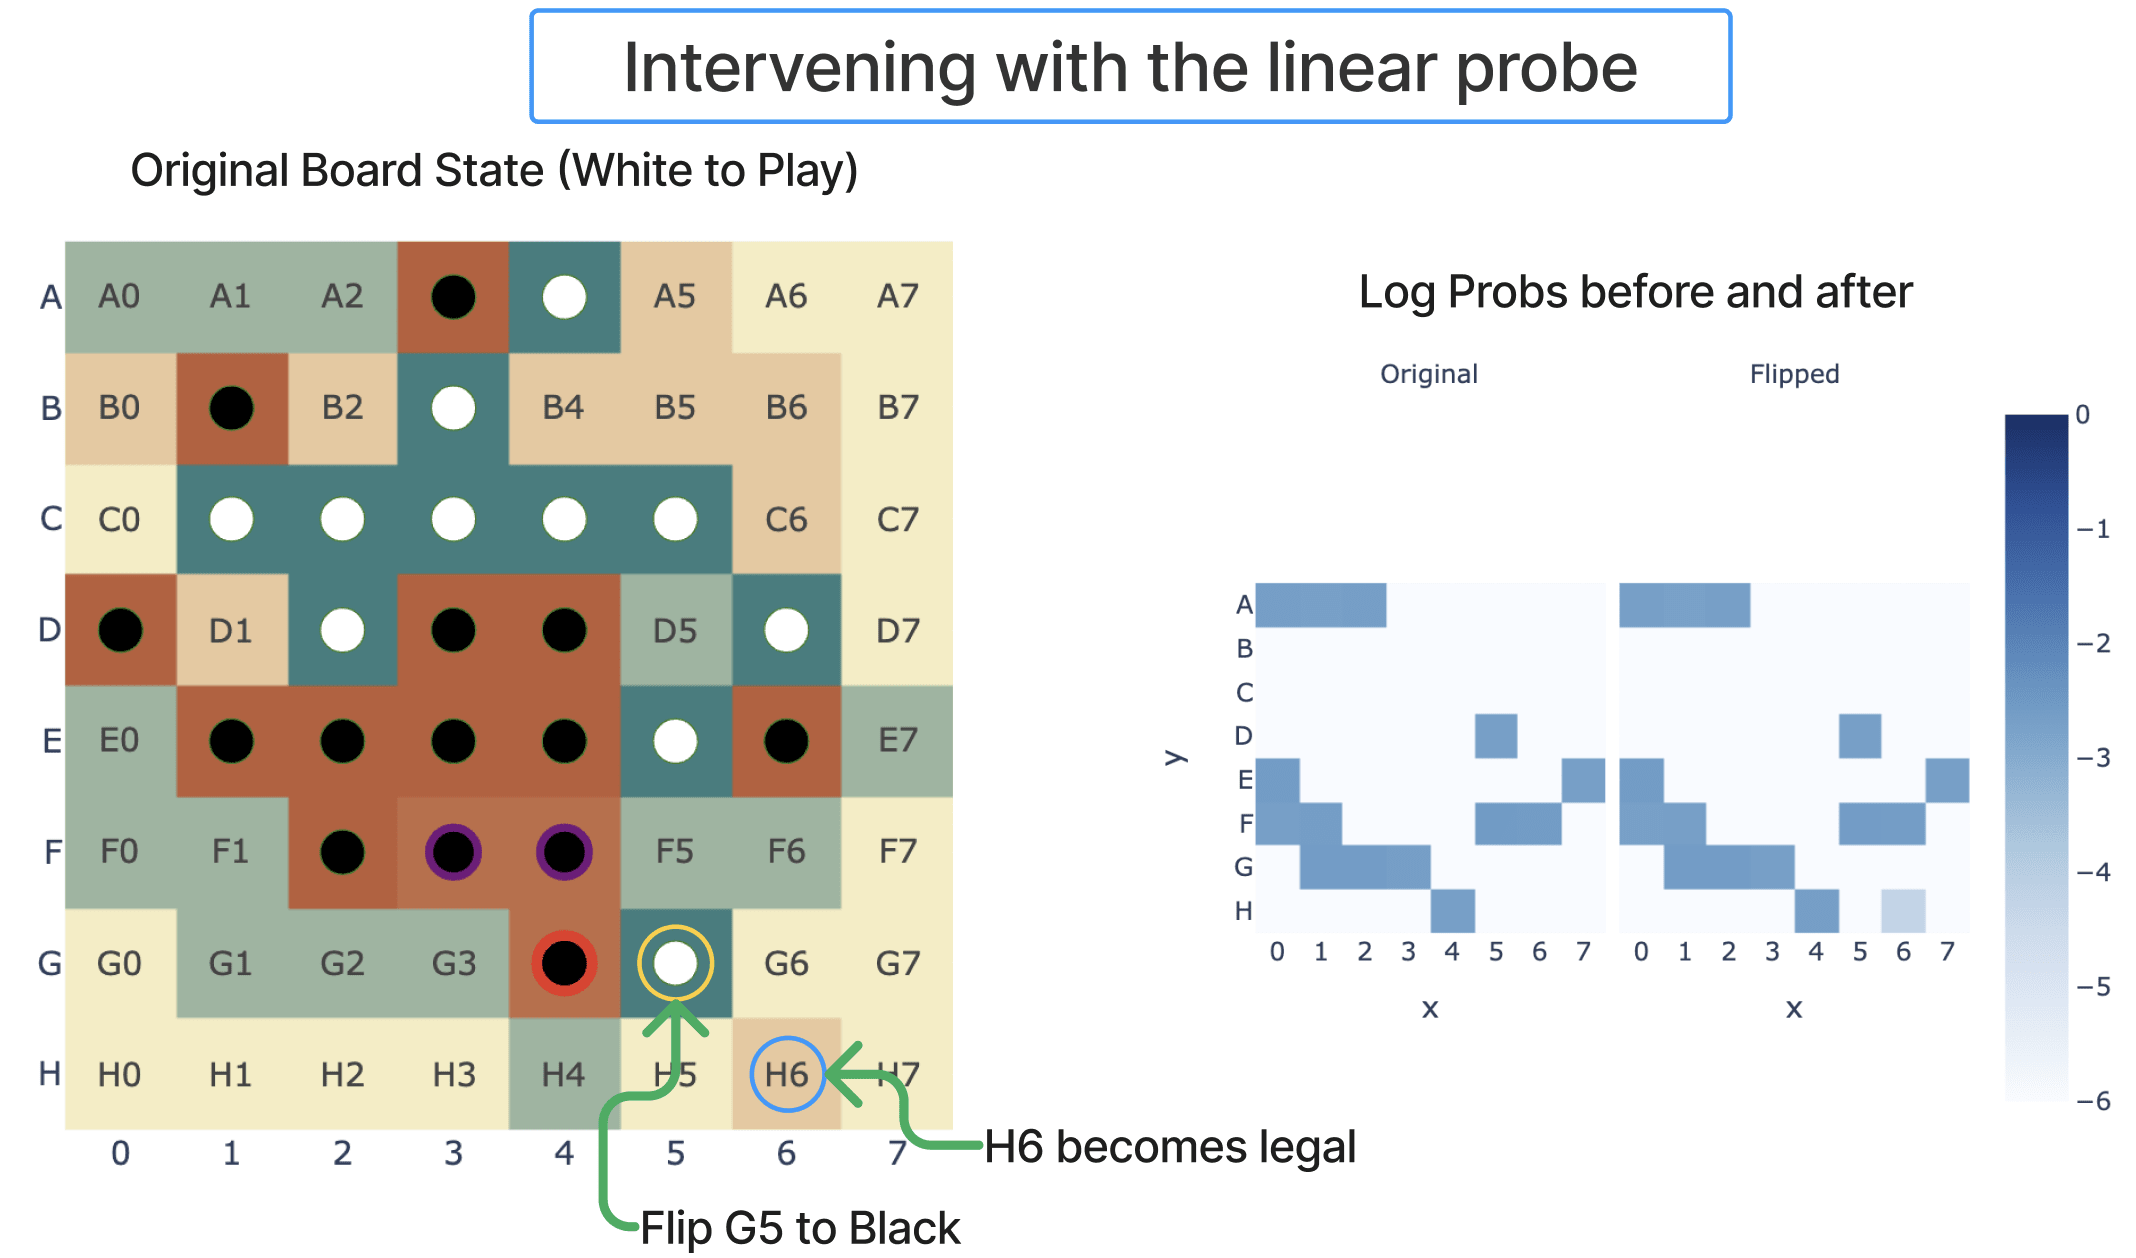
\includegraphics[width=0.7\textwidth]{othello_gpt.png}
    \captionof{figure}{Nghiên cứu Othello-GPT cho thấy một mô hình Transformer, chỉ được huấn luyện trên chuỗi nước đi, đã tự học cách biểu diễn trạng thái của bàn cờ bên trong nó.}
    \label{fig:othello_gpt}
\end{center}

\subsection{Hướng nghiên cứu và Tiềm năng}
\label{ssec:world_models_future}
Việc các LLM có thể xây dựng mô hình thế giới nội tại mở ra những hướng đi cực kỳ hứa hẹn cho tương lai của AI.

\subsubsection{Cải thiện khả năng Suy luận và Lập kế hoạch}
\begin{itemize}
    \item Nếu một Tác tử AI có một mô hình thế giới nội tại tốt, nó có thể thực hiện "mô phỏng trong tâm trí" (mental simulation).
    \item Trước khi thực hiện một hành động trong thế giới thực, nó có thể "chạy thử" hành động đó trên mô hình thế giới của mình để dự đoán kết quả.
    \item Điều này cho phép nó lập kế hoạch một cách hiệu quả hơn nhiều, lường trước các hậu quả, và tránh các sai lầm tốn kém, tương tự như cách con người suy nghĩ "nếu... thì...".
\end{itemize}

\subsubsection{Mô hình Thế giới Đa phương thức}
\begin{itemize}
    \item Hướng nghiên cứu hiện tại đang tập trung vào việc xây dựng các mô hình thế giới không chỉ từ văn bản, mà còn từ \textbf{video}.
    \item Bằng cách xem hàng triệu giờ video, một mô hình có thể học được các quy luật vật lý trực quan (intuitive physics) -- ví dụ, một vật thể không thể đi xuyên qua vật thể khác, trọng lực làm cho mọi thứ rơi xuống.
    \item Các mô hình như \textbf{Sora} của OpenAI, có khả năng sinh ra các video cực kỳ thực tế và nhất quán về mặt vật lý, được cho là một bước tiến lớn trong việc xây dựng các mô hình thế giới có khả năng mô phỏng.
\end{itemize}

\subsubsection{Hướng tới Trí tuệ Nhân tạo Tổng quát (AGI)}
\begin{itemize}
    \item Nhiều nhà nghiên cứu hàng đầu tin rằng khả năng xây dựng và sử dụng các mô hình thế giới là một trong những thành phần cốt lõi của trí thông minh thực sự.
    \item Một hệ thống AGI trong tương lai có thể sẽ bao gồm một LLM lớn đóng vai trò là "giao diện" ngôn ngữ, kết hợp với một mô hình thế giới mạnh mẽ cho phép nó hiểu sâu, suy luận, và lập kế hoạch trong một môi trường phức tạp.
\end{itemize}

Mặc dù vẫn còn là một lĩnh vực đầy tranh cãi và câu hỏi mở, giả thuyết về Mô hình Thế giới cung cấp một lăng kính mạnh mẽ để hiểu về những khả năng đáng kinh ngạc của LLM. Nó gợi ý rằng chúng ta có thể đang vô tình xây dựng được những thứ phức tạp hơn nhiều so với những gì chúng ta nghĩ ban đầu, mở ra một tương lai đầy tiềm năng cho các hệ thống AI có khả năng lý luận và tương tác với thế giới một cách sâu sắc.
% % !TEX root = ../main.tex
% File: chapters_part1/chap6_6.tex (đã chuyển sang chương 6)
% Nội dung cho Phần 6.6: Các Kỹ thuật Biểu diễn Nâng cao cho Truy xuất


\section{Các Kỹ thuật Biểu diễn Nâng cao cho Truy xuất}
\label{sec:advanced_representation_retrieval}

\subsection{Biểu diễn Đa ngôn ngữ (Cross-lingual Embeddings)}
\label{ssec:cross_lingual_embeddings}

\subsubsection*{Vấn đề}
Các mô hình như Word2Vec hay GloVe khi huấn luyện riêng biệt trên từng ngôn ngữ sẽ tạo ra các không gian vector độc lập, không có mối liên hệ.  
Ví dụ: vector của từ \textit{"máy tính"} (tiếng Việt) và \textit{"computer"} (tiếng Anh) có thể nằm ở vị trí hoàn toàn ngẫu nhiên trong hai không gian khác nhau, dù ý nghĩa giống nhau.

\subsubsection*{Mục tiêu}
\textbf{Biểu diễn đa ngôn ngữ} tìm cách xây dựng một \textbf{không gian vector chung (shared vector space)}, trong đó các từ/câu có nghĩa tương đương ở các ngôn ngữ khác nhau sẽ được ánh xạ gần nhau. Điều này cho phép:
\begin{itemize}
    \item Tìm kiếm thông tin đa ngôn ngữ (cross-lingual information retrieval).
    \item Phân loại tài liệu nhiều ngôn ngữ với một mô hình duy nhất.
    \item Dịch máy hoặc gợi ý từ/câu dựa trên ngữ nghĩa thay vì chỉ dựa vào từ vựng.
\end{itemize}

\begin{tcolorbox}[
    title={Một "Ngôn ngữ chung" của các Vector},
    colback=green!5!white, colframe=green!50!black, fonttitle=\bfseries
]
Hãy tưởng tượng một không gian nơi vector của \textit{"mèo"} (vi), \textit{"cat"} (en), \textit{"neko"} (ja) và \textit{"gato"} (es) đều hội tụ về cùng một vùng lân cận. Đây là sức mạnh của biểu diễn đa ngôn ngữ — tạo ra một “cầu nối” toán học giữa các ngôn ngữ tự nhiên.
\end{tcolorbox}

\subsubsection*{Các hướng tiếp cận chính}
\begin{enumerate}
    \item \textbf{Mapping-based (Học ma trận ánh xạ)}  
    Huấn luyện một ma trận $W$ sao cho khi nhân với embedding của ngôn ngữ nguồn, ta nhận được embedding “khớp” với ngôn ngữ đích:  
    \[
    W \cdot E_{\text{src}} \approx E_{\text{tgt}}
    \]
    - \textbf{MUSE} (Lample et al.): Tìm $W$ bằng cách tối ưu khoảng cách giữa các cặp từ song ngữ. Có thể:
        - \textit{Giám sát}: Dùng từ điển song ngữ nhỏ.
        - \textit{Phi giám sát}: Sử dụng huấn luyện đối nghịch (adversarial training) để khớp phân phối embedding.
    
    \item \textbf{Joint training (Huấn luyện chung nhiều ngôn ngữ)}  
    Huấn luyện một encoder duy nhất trên dữ liệu song song nhiều ngôn ngữ để ép embedding về chung một không gian.
    - \textbf{LASER}: Sử dụng BiLSTM encoder + max-pooling, huấn luyện trên hơn 90 ngôn ngữ.
    - \textbf{LaBSE}: Thay BiLSTM bằng Transformer (BERT), tối ưu độ tương đồng cosine giữa cặp câu dịch chuẩn và giảm độ tương đồng với cặp câu ngẫu nhiên.
    
    \item \textbf{Multilingual Language Models}  
    Huấn luyện mô hình ngôn ngữ đa ngôn ngữ trực tiếp:
    - \textbf{mBERT}, \textbf{XLM-R}: Học embedding từ pretraining masked language modeling trên nhiều ngôn ngữ.
    - \textbf{mT5}, \textbf{BLOOMZ}: Mô hình sinh đa ngôn ngữ, có thể dùng embedding tầng encoder.
\end{enumerate}

\subsubsection*{Thách thức}
\begin{itemize}
    \item \textbf{Polysemy}: Từ đa nghĩa có thể gây nhầm lẫn nếu không có ngữ cảnh.
    \item \textbf{Resource imbalance}: Một số ngôn ngữ có ít dữ liệu song song → khó huấn luyện tốt.
    \item \textbf{Domain shift}: Khác biệt miền dữ liệu (ví dụ: tin tức vs hội thoại) làm giảm chất lượng ánh xạ.
\end{itemize}

\subsubsection*{Ứng dụng minh hoạ}
\begin{itemize}
    \item Tìm kiếm học thuật: Gõ từ khoá tiếng Việt nhưng vẫn tìm được bài báo tiếng Anh/Nhật.
    \item Phân tích cảm xúc đa ngôn ngữ: Một mô hình duy nhất cho nhiều ngôn ngữ.
    \item Dịch máy zero-shot: Mô hình chưa từng thấy cặp ngôn ngữ nhưng vẫn dịch được nhờ embedding chung.
\end{itemize}


\subsection{Biểu diễn Thưa và Tối ưu cho Truy xuất (Sparse \& Retriever-specific Embeddings)}
\label{ssec:sparse_retriever_embeddings}

\subsubsection*{Bối cảnh}
Trong tìm kiếm thông tin (Information Retrieval – IR), có hai trường phái chính:
\begin{itemize}
    \item \textbf{Sparse retrieval} (ví dụ: TF-IDF, BM25): Biểu diễn tài liệu và truy vấn như vector thưa với số chiều bằng kích thước từ vựng. Nhanh, dễ lập chỉ mục, nhưng yếu về ngữ nghĩa – chỉ khớp chính xác từ khóa.
    \item \textbf{Dense retrieval} (ví dụ: BERT embeddings): Biểu diễn tài liệu và truy vấn bằng vector dày đặc, có khả năng nắm bắt ý nghĩa, nhưng tìm kiếm trên hàng triệu vector tốn tài nguyên (phải dùng ANN – Approximate Nearest Neighbor).
\end{itemize}

\subsubsection*{Vấn đề}
Dense embeddings tuy mạnh về ngữ nghĩa nhưng:
\begin{enumerate}
    \item Bỏ lỡ các khớp từ khóa chính xác (\textit{exact match}), đặc biệt quan trọng với các tên riêng, thuật ngữ kỹ thuật.
    \item Chi phí lưu trữ và tìm kiếm cao khi số tài liệu rất lớn.
\end{enumerate}

\subsubsection*{Mục tiêu}
Tạo ra các \textbf{retriever-specific embeddings} kết hợp được:
\begin{itemize}
    \item Sức mạnh khớp từ khóa của sparse retrieval.
    \item Hiểu ngữ nghĩa sâu của dense retrieval.
\end{itemize}

\subsubsection*{Các phương pháp tiêu biểu}
\paragraph{SPLADE (SPARse Lexical AnD Expansion model)}
\begin{itemize}
    \item Huấn luyện một Transformer (BERT/DistilBERT) để đầu ra là vector thưa có số chiều bằng kích thước từ vựng.
    \item Mỗi chiều tương ứng với một token trong từ vựng, giá trị là mức độ quan trọng (\textit{term weight}).
    \item Hỗ trợ \textbf{term expansion}: gán trọng số cho cả từ không xuất hiện trong văn bản nhưng có liên quan ngữ nghĩa.
    \item Hàm loss: thường là \textit{margin ranking loss} hoặc \textit{cross-entropy loss} trên cặp truy vấn–tài liệu (relevant vs non-relevant).
    \item Ưu điểm: tương thích với \textbf{inverted index}, tốc độ truy xuất gần như BM25, nhưng giàu ngữ nghĩa hơn.
\end{itemize}

\paragraph{ColBERT (Contextualized Late Interaction over BERT)}
\begin{itemize}
    \item Thay vì nén cả tài liệu thành một vector, ColBERT tạo embedding dày đặc cho từng token.
    \item Khi truy vấn, với mỗi token trong câu hỏi, tính độ tương đồng tối đa với tất cả token embedding của tài liệu.
    \item Hàm loss: tối đa hoá độ tương đồng giữa truy vấn và tài liệu liên quan, đồng thời giảm độ tương đồng với tài liệu không liên quan.
    \item Ưu điểm: giữ được chi tiết cấp từ, cho độ chính xác cao hơn dense retriever thuần.
    \item Nhược điểm: tốn bộ nhớ và chậm hơn do số lượng embedding lớn.
\end{itemize}

\subsubsection*{Kết hợp trong hệ thống RAG}
\begin{itemize}
    \item \textbf{SPLADE}: tốt để mở rộng tập ứng viên (candidate set) nhờ độ phủ cao và khả năng truy xuất nhanh.
    \item \textbf{ColBERT}: tốt để rerank tập ứng viên nhỏ, nhờ giữ được ngữ cảnh chi tiết.
    \item Chiến lược phổ biến: SPLADE \(\rightarrow\) lấy top-1000 tài liệu \(\rightarrow\) ColBERT rerank top-50 \(\rightarrow\) đưa vào LLM.
\end{itemize}

\subsubsection*{Thách thức}
\begin{itemize}
    \item Tối ưu tốc độ khi kết hợp nhiều tầng retriever.
    \item Cân bằng giữa recall (độ phủ) và precision (độ chính xác).
    \item Chi phí lưu trữ embedding lớn với mô hình late-interaction.
\end{itemize}

\bigskip
\hrule
\bigskip

\begin{center}
    \textbf{\Large KẾT THÚC CHƯƠNG 6}
\end{center}

\textit{Chúng ta đã đi đến cuối hành trình khám phá các hệ thống AI tiên tiến. Chương này đã mở rộng tầm nhìn của chúng ta vượt ra ngoài một LLM đơn lẻ, cho thấy cách kết hợp nó với các nguồn kiến thức bên ngoài (RAG), các phương thức khác (Multimodality), và các công cụ (Agentic Systems) để tạo ra các giải pháp mạnh mẽ. Chúng ta cũng đã tìm hiểu các kỹ thuật tối ưu hóa để đưa những mô hình này vào thực tế và suy ngẫm về khái niệm "Mô hình Thế giới". Chúng ta đã xây dựng nên những hệ thống AI vô cùng phức tạp và mạnh mẽ. Nhưng một câu hỏi tối quan trọng vẫn còn đó: Làm thế nào để chúng ta đo lường và so sánh chúng một cách khoa học? Liệu mô hình A có thực sự tốt hơn mô hình B không, và dựa trên tiêu chí nào? Chương cuối cùng của Phần 1 sẽ đi sâu vào lý thuyết và thực hành của việc đánh giá, cung cấp cho chúng ta những công cụ cần thiết để định lượng sự tiến bộ và hiểu rõ những giới hạn của các mô hình này.}

% \chapter{CÁC KIẾN TRÚC MẠNG NƠ-RON KINH ĐIỂN}
\label{chap:deep_learning_architectures}

Chào mừng bạn đến với kỷ nguyên học sâu của NLP. Trong chương 2, chúng ta đã thấy các mô hình thống kê như N-gram có thể nắm bắt các phụ thuộc cục bộ, nhưng lại bất lực trước các mối quan hệ tầm xa. Cuộc cách mạng word embedding đã cho chúng ta các vector từ mang đầy ngữ nghĩa, nhưng làm thế nào để kết hợp chúng lại nhằm hiểu được ý nghĩa của cả một câu hay một đoạn văn?

Chương này sẽ giới thiệu các kiến trúc mạng nơ-ron nền tảng được thiết kế đặc biệt để xử lý dữ liệu dạng chuỗi như ngôn ngữ tự nhiên. Những kiến trúc này không chỉ đơn thuần "nhìn" vào các từ một cách riêng lẻ, mà còn có khả năng "ghi nhớ" và "lý luận" dựa trên thông tin đã xử lý trước đó, cho phép chúng nắm bắt được ngữ cảnh và các phụ thuộc phức tạp trong câu.
% % !TEX root = ../main.tex
% File: chapters_part1/chap7_1.tex
% Nội dung cho Chương 7, Phần 1


\section{Các Metric kinh điển}
\label{sec:classic_metrics}

Đây là những công cụ đầu tiên và cơ bản nhất trong bộ công cụ của bất kỳ nhà thực hành NLP nào. Mỗi metric được thiết kế để đo lường một khía cạnh cụ thể của hiệu năng mô hình.

\subsection{Perplexity: Đo lường chất lượng của Mô hình Ngôn ngữ}
\label{ssec:perplexity}
\begin{itemize}
    \item \textbf{Dùng cho tác vụ nào?} Đánh giá chất lượng nội tại của các \textbf{Mô hình Ngôn ngữ (Language Models)} (ví dụ: các mô hình được huấn luyện để dự đoán từ tiếp theo).
    \item \textbf{Trực giác cốt lõi:} Một mô hình ngôn ngữ tốt là mô hình \textbf{ít "ngạc nhiên" (less surprised)} hơn khi nhìn thấy một câu văn thực tế. Perplexity (PPL), hay còn gọi là Độ bối rối, chính là một cách để định lượng sự "ngạc nhiên" này. \textbf{Perplexity càng thấp, mô hình càng tốt}.
    \item \textbf{Cơ chế hoạt động:} Perplexity có mối quan hệ trực tiếp với hàm mất mát Cross-Entropy. Đối với một chuỗi văn bản $W = (w_1, w_2, \dots, w_N)$, Perplexity được định nghĩa là:
        \begin{equation}
            \text{PPL}(W) = \sqrt[N]{\frac{1}{P(w_1, w_2, \dots, w_N)}} = \left( \prod_{i=1}^{N} \frac{1}{P(w_i|w_1, \dots, w_{i-1})} \right)^{1/N}
            \label{eq:perplexity}
        \end{equation}
        Về mặt toán học, nó là nghịch đảo của xác suất trung bình trên mỗi từ (được lấy căn bậc $N$).
    \item \textbf{Hạn chế:}
        \begin{itemize}
            \item Chỉ đo lường khả năng dự đoán xác suất, không trực tiếp đo lường chất lượng ngữ nghĩa hay sự mạch lạc của văn bản được sinh ra.
            \item Rất nhạy cảm với kích thước từ vựng. Không thể so sánh Perplexity của hai mô hình có từ vựng khác nhau.
        \end{itemize}
\end{itemize}

\subsection{Precision, Recall, và F1-Score: Nền tảng của các bài toán Phân loại}
\label{ssec:f1_score}
Đây là bộ ba metric không thể thiếu cho hầu hết các bài toán \textbf{phân loại (classification)} và \textbf{trích xuất thông tin (information extraction)} như NER.

\subsubsection{Các thành phần cơ bản}
Để hiểu bộ ba này, chúng ta cần định nghĩa bốn kết quả có thể xảy ra khi phân loại một điểm dữ liệu:
\begin{itemize}
    \item \textbf{True Positive (TP):} Dự đoán là \textbf{Dương tính}, và thực tế là \textbf{Dương tính}. (Dự đoán đúng)
    \item \textbf{True Negative (TN):} Dự đoán là \textbf{Âm tính}, và thực tế là \textbf{Âm tính}. (Dự đoán đúng)
    \item \textbf{False Positive (FP):} Dự đoán là \textbf{Dương tính}, nhưng thực tế là \textbf{Âm tính}. (Lỗi Loại I - "báo động giả")
    \item \textbf{False Negative (FN):} Dự đoán là \textbf{Âm tính}, nhưng thực tế là \textbf{Dương tính}. (Lỗi Loại II - "bỏ sót")
\end{itemize}

\begin{center}
    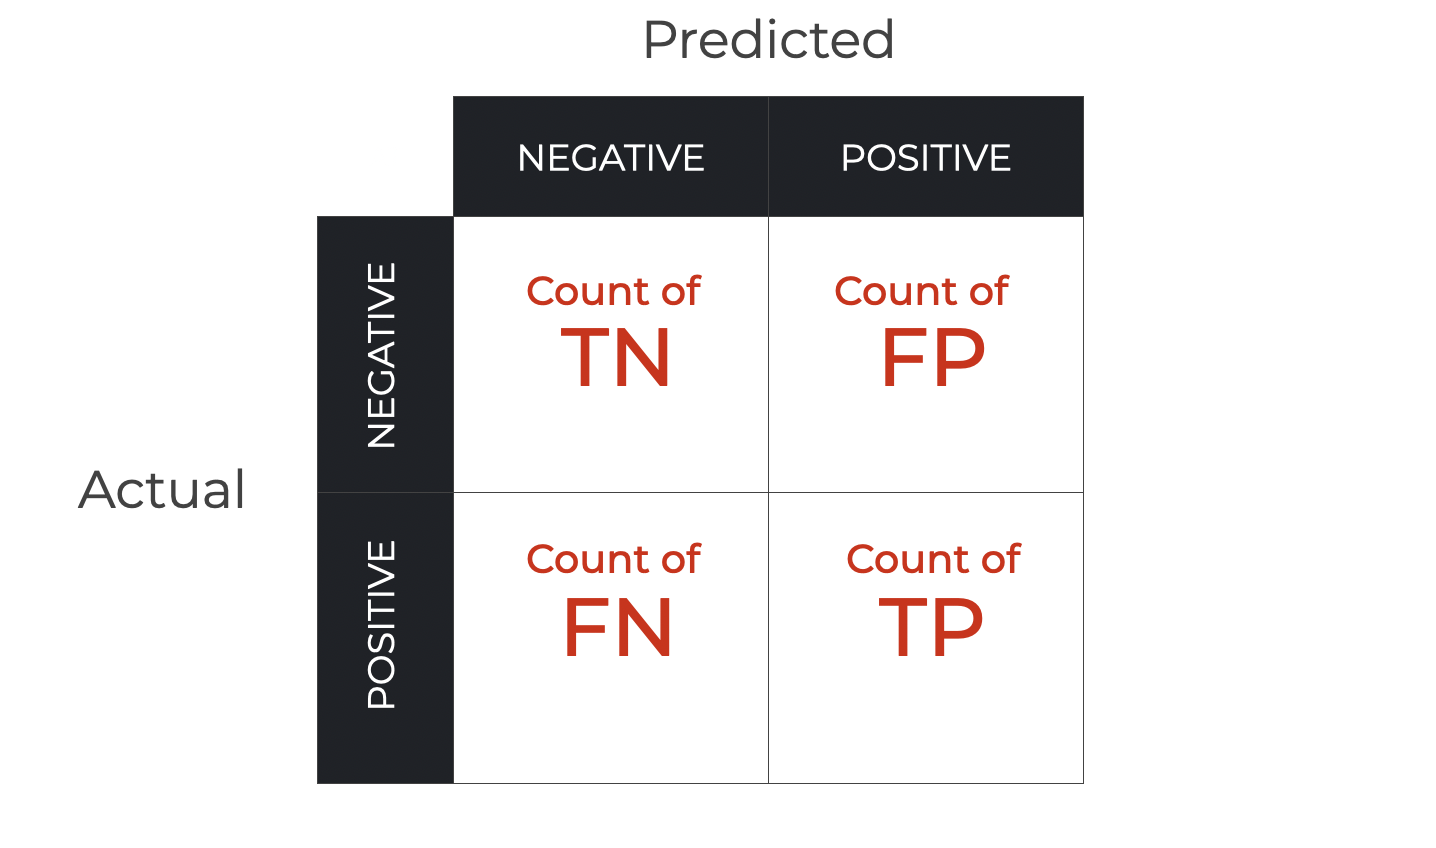
\includegraphics[width=0.6\textwidth]{confusion_matrix.png}
    \captionof{figure}{Ma trận nhầm lẫn (Confusion Matrix) minh họa bốn kết quả của một bài toán phân loại nhị phân.}
    \label{fig:confusion_matrix}
\end{center}

\subsubsection{Định nghĩa các Metric}
\paragraph{Precision (Độ chính xác)}
\begin{itemize}
    \item \textbf{Câu hỏi nó trả lời:} "Trong số tất cả những gì mô hình dự đoán là Dương tính, có bao nhiêu cái thực sự là Dương tính?"
    \item \textbf{Công thức:}
        $$ \text{Precision} = \frac{\text{TP}}{\text{TP} + \text{FP}} $$
    \item \textbf{Mục tiêu:} Tối đa hóa Precision có nghĩa là cố gắng giảm thiểu số lượng báo động giả (FP). Rất quan trọng trong các ứng dụng như phát hiện spam (thà bỏ sót một email spam còn hơn là đưa một email quan trọng vào hòm thư rác).
\end{itemize}

\paragraph{Recall (Độ phủ, hay Độ nhạy)}
\begin{itemize}
    \item \textbf{Câu hỏi nó trả lời:} "Trong số tất cả những cái thực sự là Dương tính, mô hình đã tìm thấy được bao nhiêu cái?"
    \item \textbf{Công thức:}
        $$ \text{Recall} = \frac{\text{TP}}{\text{TP} + \text{FN}} $$
    \item \textbf{Mục tiêu:} Tối đa hóa Recall có nghĩa là cố gắng giảm thiểu số lượng bỏ sót (FN). Rất quan trọng trong các ứng dụng như chẩn đoán y tế (thà chẩn đoán nhầm một người khỏe mạnh là có bệnh còn hơn là bỏ sót một người thực sự có bệnh).
\end{itemize}

\paragraph{F1-Score (Điểm F1)}
\begin{itemize}
    \item \textbf{Vấn đề:} Precision và Recall thường có sự đánh đổi (trade-off). Một mô hình rất "cẩn trọng" có thể có Precision cao nhưng Recall thấp, và ngược lại. F1-score được tạo ra để kết hợp cả hai thành một chỉ số duy nhất.
    \item \textbf{Công thức:} F1-score là trung bình điều hòa (harmonic mean) của Precision và Recall.
        $$ \text{F1-Score} = 2 \cdot \frac{\text{Precision} \cdot \text{Recall}}{\text{Precision} + \text{Recall}} $$
    \item \textbf{Mục tiêu:} F1-score cao khi cả Precision và Recall đều cao. Nó là một thước đo cân bằng, được sử dụng rộng rãi trong các tác vụ như NER, nơi chúng ta quan tâm đến cả việc không nhận dạng sai và không bỏ sót thực thể.
\end{itemize}
Khi đánh giá trên nhiều lớp, người ta thường tính `macro-F1` (tính F1 cho mỗi lớp rồi lấy trung bình) hoặc `micro-F1` (tính tổng TP, FP, FN trên tất cả các lớp rồi mới tính F1).

\subsection{BLEU: Đánh giá Dịch máy}
\label{ssec:bleu}
\begin{itemize}
    \item \textbf{Dùng cho tác vụ nào?} Chủ yếu là \textbf{Dịch máy (Machine Translation)}, nhưng đôi khi cũng dùng cho các tác vụ sinh văn bản khác.
    \item \textbf{Trực giác cốt lõi:} Một bản dịch tốt nên có nhiều \textbf{N-gram trùng lặp} với các bản dịch tham khảo chất lượng cao do con người tạo ra.
    \item \textbf{Cơ chế hoạt động:} BLEU (Bilingual Evaluation Understudy) tính toán một điểm số dựa trên hai yếu tố:
        \begin{enumerate}
            \item \textbf{Độ chính xác N-gram đã được sửa đổi (Modified N-gram Precision):} Tính toán tỷ lệ các N-gram (thường từ 1-gram đến 4-gram) trong câu do máy dịch tạo ra cũng xuất hiện trong các câu tham khảo. Nó được "sửa đổi" để ngăn mô hình lặp lại một từ đúng nhiều lần để gian lận điểm.
            \item \textbf{Hình phạt cho câu ngắn (Brevity Penalty - BP):} Nếu câu do máy dịch tạo ra ngắn hơn đáng kể so với các câu tham khảo, nó sẽ bị phạt. Điều này ngăn mô hình chỉ sinh ra một vài từ rất chính xác để có Precision cao.
        \end{enumerate}
        $$ \text{BLEU} = \text{BP} \cdot \exp\left(\sum_{n=1}^{N} w_n \log p_n\right) $$
        Trong đó $p_n$ là độ chính xác của n-gram, và $w_n$ thường là $1/N$.
    \item \textbf{Hạn chế:}
        \begin{itemize}
            \item \textbf{Chỉ quan tâm đến Precision, không quan tâm đến Recall:} Nó không phạt nếu bản dịch bỏ sót các thông tin quan trọng.
            \item \textbf{Không hiểu ngữ nghĩa:} Một bản dịch có thể dùng từ đồng nghĩa hoàn hảo nhưng vẫn bị điểm BLEU thấp nếu không khớp chính xác N-gram.
            \item \textbf{Gặp khó khăn với trật tự từ và sự sáng tạo:} Không đánh giá tốt các bản dịch có cấu trúc câu khác biệt nhưng vẫn đúng.
        \end{itemize}
\end{itemize}

\subsection{ROUGE: Đánh giá Tóm tắt Văn bản}
\label{ssec:rouge}
\begin{itemize}
    \item \textbf{Dùng cho tác vụ nào?} Chủ yếu là \textbf{Tóm tắt văn bản (Summarization)}.
    \item \textbf{Trực giác cốt lõi:} ROUGE (Recall-Oriented Understudy for Gisting Evaluation) hoạt động ngược lại với BLEU. Nó cho rằng một bản tóm tắt tốt nên \textbf "bao phủ" được các N-gram quan trọng có trong các bản tóm tắt tham khảo của con người.
    \item \textbf{Cơ chế hoạt động:} ROUGE là một họ các metric, trong đó phổ biến nhất là:
        \begin{itemize}
            \item \textbf{ROUGE-N:} Dựa trên sự trùng lặp N-gram, nhưng tính toán dựa trên \textbf{Recall}.
                $$ \text{ROUGE-N} = \frac{\text{Số N-gram trong tham khảo cũng xuất hiện trong tóm tắt máy}}{\text{Tổng số N-gram trong tham khảo}} $$
                Thường dùng `ROUGE-1` (unigram) và `ROUGE-2` (bigram).
            \item \textbf{ROUGE-L:} Dựa trên \textbf{Chuỗi con chung dài nhất (Longest Common Subsequence - LCS)}. Nó không yêu cầu các từ phải liền kề nhau, do đó nắm bắt được sự tương đồng về trật tự từ tốt hơn.
        \end{itemize}
    \item \textbf{Hạn chế:} Tương tự như BLEU, ROUGE cũng chỉ dựa trên sự khớp bề mặt của từ và không hiểu được ngữ nghĩa sâu sắc. Một bản tóm tắt có thể diễn đạt lại ý tưởng một cách hoàn hảo nhưng vẫn bị điểm ROUGE thấp.
\end{itemize}

Mặc dù có nhiều hạn chế, các metric kinh điển này vẫn được sử dụng rộng rãi vì chúng tự động, nhanh chóng và cung cấp một thước đo khách quan (dù không hoàn hảo) để so sánh các mô hình với nhau trong quá trình phát triển.
% % !TEX root = ../main.tex
% File: chapters_part1/chap7_2.tex
% Nội dung cho Chương 7, Phần 2

\section{Các Benchmark Kinh điển và Hiện đại}
\label{sec:benchmarks}

Một metric riêng lẻ chỉ đo lường một khía cạnh của mô hình. Để có một đánh giá toàn diện, cộng đồng nghiên cứu đã tạo ra các \textbf{benchmark} -- những bộ sưu tập các bộ dữ liệu và tác vụ được tiêu chuẩn hóa. Các benchmark đóng vai trò như những "kỳ thi Olympic" cho các mô hình NLP, cho phép các nhà nghiên cứu so sánh một cách công bằng và theo dõi sự tiến bộ của toàn ngành.

Sự phát triển của các benchmark cũng phản ánh sự tiến hóa của chính các mô hình NLP.

\subsection{Kỷ nguyên Pre-LLM: GLUE và SuperGLUE}
\label{ssec:pre_llm_benchmarks}
Trước khi các LLM lớn với khả năng zero-shot ra đời, các mô hình (như BERT) thường được đánh giá bằng cách tinh chỉnh (fine-tune) trên một loạt các tác vụ Hiểu Ngôn ngữ Tự nhiên (NLU) đa dạng. GLUE và SuperGLUE là hai benchmark tiêu biểu nhất cho kỷ nguyên này.

\subsubsection{GLUE: Một Bài kiểm tra Năng lực Ngôn ngữ Tổng quát}
\begin{itemize}
    \item \textbf{Tên đầy đủ:} General Language Understanding Evaluation.
    \item \textbf{Triết lý:} Một mô hình thực sự hiểu ngôn ngữ phải hoạt động tốt trên nhiều loại tác vụ khác nhau, từ suy luận, phân tích cảm xúc, đến nhận dạng sự tương đồng.
    \item \textbf{Cấu trúc:} GLUE bao gồm 9 tác vụ NLU khác nhau, được nhóm thành các loại:
        \begin{itemize}
            \item \textbf{Suy luận Ngôn ngữ Tự nhiên (NLI):} MNLI, QNLI, RTE.
            \item \textbf{Tương đồng Ngữ nghĩa và Diễn giải:} MRPC, QQP, STS-B.
            \item \textbf{Phân loại câu đơn:} SST-2 (cảm xúc), CoLA (tính đúng ngữ pháp).
        \end{itemize}
    \item \textbf{Đánh giá:} Một mô hình được fine-tune riêng cho từng tác vụ. Điểm số cuối cùng là điểm trung bình trên tất cả các tác vụ.
    \item \textbf{Tác động:} GLUE đã trở thành một "thước đo vàng" để đánh giá các mô hình như BERT, RoBERTa. Tuy nhiên, các mô hình nhanh chóng đạt đến và \textbf{vượt qua cả hiệu năng của con người} trên benchmark này vào khoảng năm 2019, cho thấy nó đã trở nên quá "dễ".
\end{itemize}

\subsubsection{SuperGLUE: Nâng cấp Độ khó}
\begin{itemize}
    \item \textbf{Động lực:} Do GLUE đã bị "chinh phục", SuperGLUE được tạo ra với các tác vụ khó hơn, đòi hỏi khả năng suy luận phức tạp hơn.
    \item \textbf{Cấu trúc:} Nó cũng là một bộ sưu tập các tác vụ đa dạng, nhưng tập trung nhiều hơn vào:
        \begin{itemize}
            \item \textbf{Hỏi-đáp yêu cầu suy luận:} BoolQ, MultiRC.
            \item \textbf{Suy luận nhân quả:} COPA.
            \item \textbf{Giải quyết đồng tham chiếu:} WSC.
        \end{itemize}
    \item \textbf{Tác động:} SuperGLUE đã tiếp tục là một thách thức trong một thời gian, nhưng rồi các mô hình lớn hơn cũng dần chinh phục được nó. Sự bão hòa của các benchmark này cho thấy một giới hạn của mô hình fine-tuning và sự cần thiết của các phương pháp đánh giá mới.
\end{itemize}

\subsection{Kỷ nguyên LLM: Đánh giá các Khả năng Nổi trội (Emergent Abilities)}
\label{ssec:llm_benchmarks}
Với sự ra đời của các LLM có khả năng few-shot, mô hình đánh giá đã thay đổi. Thay vì fine-tuning, các benchmark mới tập trung vào việc đo lường kiến thức và khả năng suy luận của mô hình trong cài đặt zero-shot và few-shot.

\subsubsection{MMLU: Bài kiểm tra Kiến thức Đa chuyên ngành}
\begin{itemize}
    \item \textbf{Tên đầy đủ:} Massive Multitask Language Understanding.
    \item \textbf{Triết lý:} Một LLM mạnh phải có kiến thức sâu rộng trên nhiều lĩnh vực chuyên môn, tương tự như các kỳ thi chuẩn hóa của con người.
    \item \textbf{Cấu trúc:} MMLU bao gồm gần 16,000 câu hỏi trắc nghiệm được lấy từ các kỳ thi thực tế, bao phủ 57 môn học khác nhau, từ các môn cơ bản (toán tiểu học) đến các môn chuyên ngành cấp độ đại học và chuyên nghiệp (luật, y, kỹ thuật).
    \item \textbf{Đánh giá:} Các mô hình được đánh giá ở chế độ \textbf{few-shot (thường là 5-shot)}. Prompt sẽ bao gồm 5 câu hỏi và câu trả lời mẫu từ một môn học, sau đó là câu hỏi thực sự cần trả lời.
    \item \textbf{Tác động:} MMLU đã trở thành một trong những benchmark quan trọng nhất để đo lường kiến thức và khả năng suy luận của các LLM hàng đầu. Việc một mô hình đạt điểm cao trên MMLU là một minh chứng mạnh mẽ cho năng lực của nó.
\end{itemize}

\subsubsection{Big-Bench: Khám phá Giới hạn của LLMs}
\begin{itemize}
    \item \textbf{Tên đầy đủ:} Beyond the Imitation Game benchmark.
    \item \textbf{Triết lý:} Các benchmark hiện có vẫn còn hạn chế. Chúng ta cần một bộ sưu tập các tác vụ cực kỳ đa dạng và sáng tạo để thăm dò các khả năng và những điểm yếu bất ngờ của LLM.
    \item \textbf{Cấu trúc:} Một sự hợp tác khổng lồ của cộng đồng, tạo ra hơn 200 tác vụ rất đa dạng, bao gồm logic, lý luận toán học, hiểu biết vật lý trực quan, nhận biết định kiến xã hội, và nhiều tác vụ sáng tạo khác mà máy tính trước đây chưa từng làm tốt.
    \item \textbf{Đánh giá:} Chủ yếu ở chế độ \textbf{zero-shot}, để kiểm tra khả năng giải quyết vấn đề "ngay từ đầu" của mô hình.
    \item \textbf{Tác động:} Big-Bench đã giúp các nhà nghiên cứu xác định được các "khả năng nổi trội" (emergent abilities) -- các khả năng chỉ xuất hiện khi mô hình đạt đến một quy mô đủ lớn.
\end{itemize}

\subsubsection{HumanEval: Đánh giá Năng lực Sinh mã nguồn}
\begin{itemize}
    \item \textbf{Dùng cho tác vụ nào?} Đánh giá khả năng \textbf{viết và hoàn thiện mã nguồn (code generation)} của LLM.
    \item \textbf{Cấu trúc:} Bao gồm 164 bài toán lập trình. Mỗi bài toán được đưa ra dưới dạng một docstring (mô tả hàm) và một vài test case.
    \item \textbf{Đánh giá:} Mô hình được yêu cầu sinh ra phần thân của hàm. Mã nguồn được sinh ra sau đó sẽ được thực thi và kiểm tra xem nó có vượt qua được các test case hay không. Metric chính là \textbf{Pass@k}, tức là xác suất một giải pháp đúng được tạo ra trong $k$ lần thử.
    \item \textbf{Tác động:} HumanEval đã trở thành một tiêu chuẩn để đo lường năng lực lập trình của các mô hình như Codex, AlphaCode, và các LLM hiện đại khác.
\end{itemize}

\begin{center}
    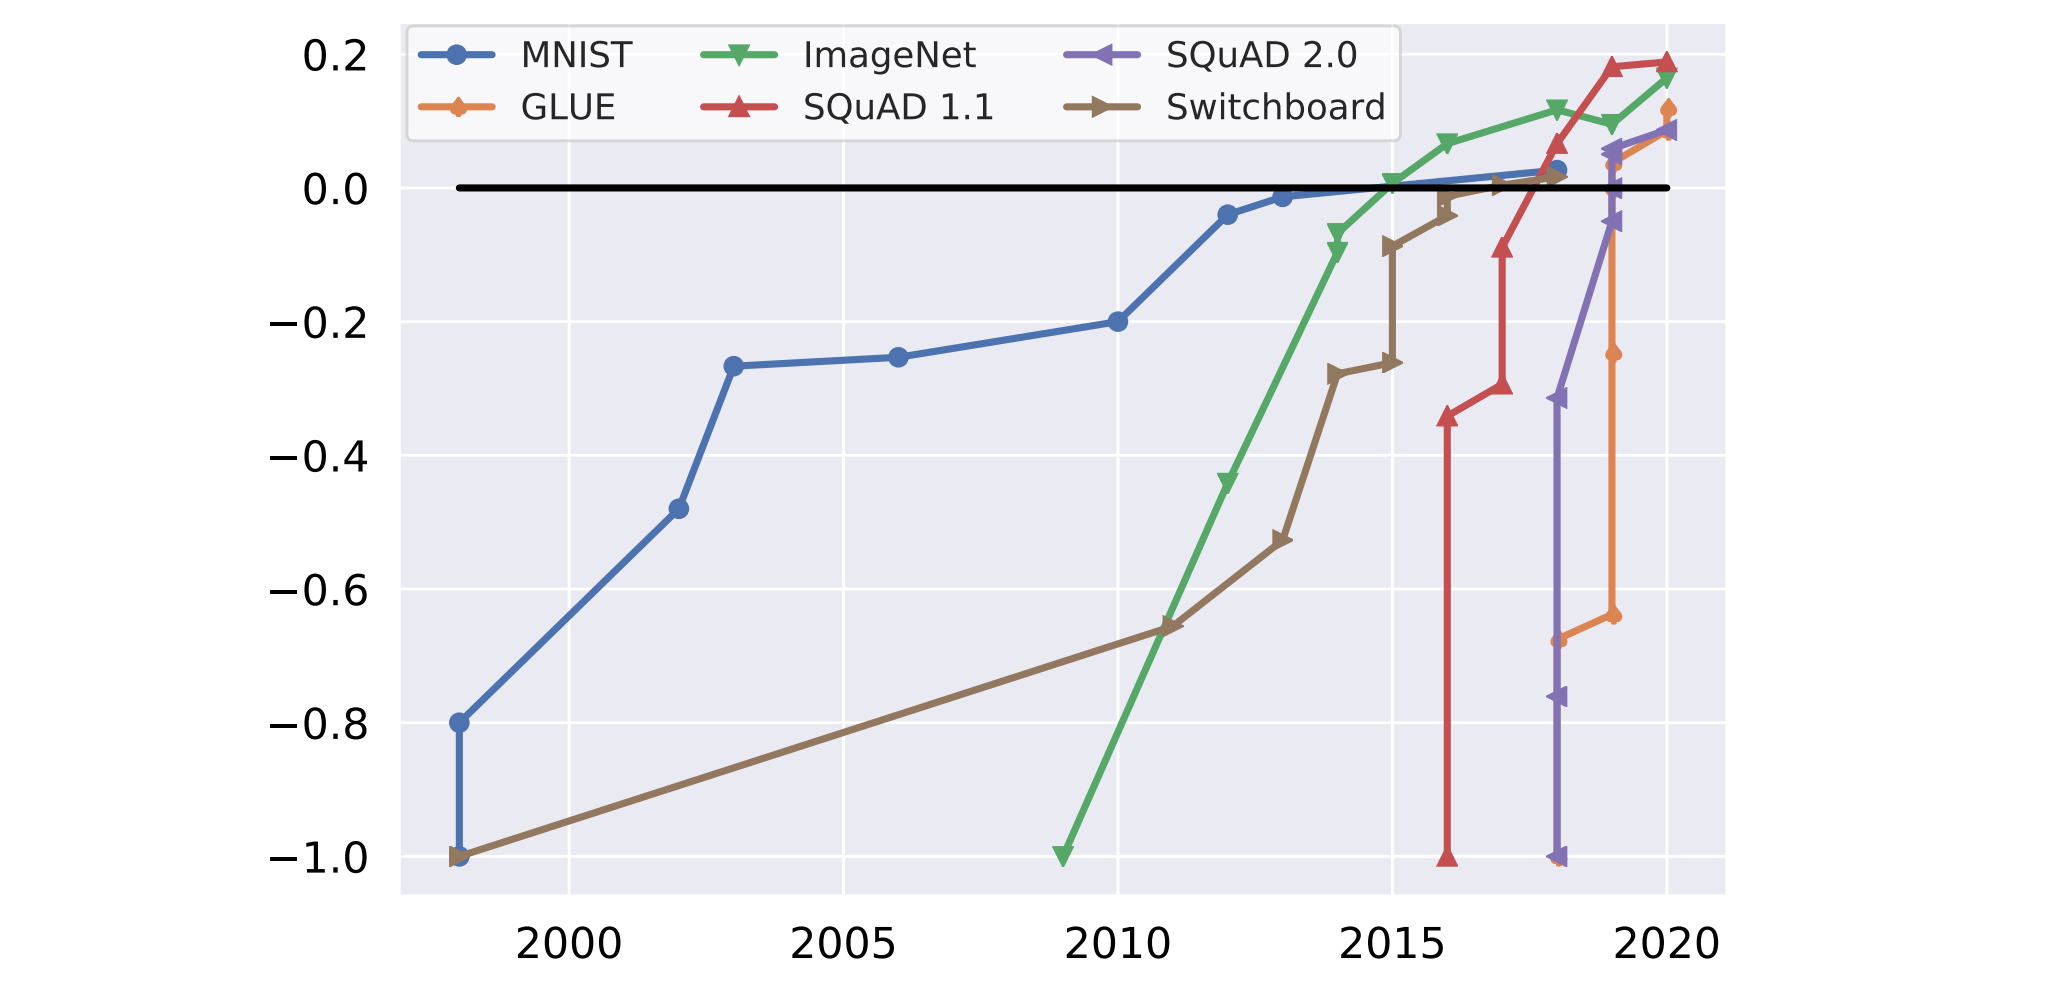
\includegraphics[width=1.0\textwidth]{llm_benchmarks_timeline.png}
    \captionof{figure}{Sơ đồ thời gian thể hiện sự phát triển của các benchmark}
    \label{fig:llm_benchmarks_timeline}
\end{center}

Việc chuyển từ các benchmark như GLUE sang MMLU/Big-Bench không chỉ là một sự thay đổi về quy mô, mà còn là một sự thay đổi cơ bản trong cách chúng ta hiểu và đo lường "trí thông minh" của các mô hình ngôn ngữ.
% % !TEX root = ../main.tex
% File: chapters_part1/chap7_3.tex
% Nội dung cho Chương 7, Phần 3

\section{Thách thức trong Đánh giá LLM}
\label{sec:llm_evaluation_challenges}

Mặc dù chúng ta đã có một bộ các metric và benchmark ngày càng tinh vi, việc đánh giá các Mô hình Ngôn ngữ Lớn vẫn là một bài toán mở với vô vàn thách thức. Việc chỉ nhìn vào một con số duy nhất trên một bảng xếp hạng (leaderboard) có thể rất sai lầm và không phản ánh được hiệu năng thực sự của mô hình trong thế giới thực.

Mục này sẽ đi sâu vào những thách thức cố hữu và những cạm bẫy tiềm ẩn trong quá trình đánh giá LLM hiện nay.

\subsection{Nhiễm bẩn Dữ liệu (Data Contamination)}
\label{ssec:data_contamination}

\begin{tcolorbox}[
    title=Vấn đề cốt lõi,
    colback=red!5!white, colframe=red!75!black, fonttitle=\bfseries
]
"Chúng ta đang kiểm tra khả năng suy luận của mô hình, hay đang kiểm tra khả năng ghi nhớ của nó?"
\end{tcolorbox}

\paragraph{Định nghĩa}
Nhiễm bẩn dữ liệu xảy ra khi dữ liệu của bộ \textbf{kiểm tra (test set)} hoặc bộ \textbf{phát triển (dev set)} của một benchmark vô tình xuất hiện trong bộ \textbf{dữ liệu huấn luyện (training set)} của mô hình.

\paragraph{Nguyên nhân}
\begin{itemize}
    \item \textbf{Dữ liệu Pre-training khổng lồ:} Các LLM được huấn luyện trên một phần lớn của Internet (ví dụ: Common Crawl). Rất có khả năng các bộ dữ liệu benchmark phổ biến (vốn cũng thường được đăng tải công khai trên các trang như GitHub, arXiv) đã nằm sẵn trong kho dữ liệu pre-training khổng lồ này.
    \item \textbf{Sự trùng lặp không chủ ý:} Ngay cả khi không có sự trùng lặp trực tiếp, các câu hỏi và câu trả lời trong benchmark có thể có các phiên bản diễn giải lại (paraphrased versions) hoặc các thảo luận về chúng nằm trên các trang web như Stack Overflow hay Reddit, và mô hình đã học được chúng.
\end{itemize}

\paragraph{Hậu quả}
\begin{itemize}
    \item \textbf{Điểm số bị thổi phồng một cách giả tạo:} Khi mô hình gặp một câu hỏi trong benchmark mà nó đã "nhìn thấy" trong quá trình huấn luyện, nó không cần phải suy luận. Nó chỉ đơn giản là "nhớ" lại và đưa ra câu trả lời. Điều này làm cho điểm số của mô hình cao hơn nhiều so với năng lực thực sự của nó.
    \item \textbf{Mất đi tính giá trị của benchmark:} Nếu một benchmark bị nhiễm bẩn nặng, nó không còn là một thước đo đáng tin cậy cho khả năng tổng quát hóa nữa.
\end{itemize}

\paragraph{Hướng giải quyết}
Đây là một vấn đề rất khó giải quyết triệt để. Các hướng tiếp cận bao gồm:
\begin{itemize}
    \item \textbf{Lọc dữ liệu cẩn thận:} Cố gắng loại bỏ các dữ liệu từ các benchmark đã biết khỏi tập pre-training.
    \item \textbf{Phát triển các benchmark mới liên tục:} Tạo ra các bộ dữ liệu mới, được giữ kín cho đến khi công bố.
    \item \textbf{Các phương pháp phát hiện nhiễm bẩn:} Phát triển các kỹ thuật để ước tính mức độ một mô hình đã "học thuộc lòng" một benchmark.
\end{itemize}

\subsection{Đánh giá bởi Con người vs. Đánh giá Tự động (Human vs. Auto Evaluation)}
\label{ssec:human_vs_auto_eval}

\subsubsection{Hạn chế của Đánh giá Tự động (Auto-Eval)}
Như đã thảo luận ở mục \ref{sec:classic_metrics}, các metric tự động như BLEU, ROUGE có những hạn chế nghiêm trọng:
\begin{itemize}
    \item \textbf{Hời hợt:} Chúng chỉ dựa trên sự trùng lặp bề mặt của từ hoặc N-gram.
    \item \textbf{Không hiểu ngữ nghĩa:} Chúng không thể đánh giá sự sáng tạo, tính mạch lạc, hay sự chính xác về mặt factual. Một câu trả lời có thể sai hoàn toàn về mặt thông tin nhưng vẫn đạt điểm ROUGE cao nếu nó sử dụng lại các từ trong tài liệu tham khảo.
    \item \textbf{Không đo lường được các khía cạnh tinh tế:} Không thể đo lường được "tính hữu ích", "sự thú vị", hay "mức độ an toàn" của một câu trả lời.
\end{itemize}

\subsubsection{Ưu điểm và Thách thức của Đánh giá bởi Con người (Human-Eval)}
\begin{itemize}
    \item \textbf{Tiêu chuẩn vàng:} Đánh giá của con người là tiêu chuẩn vàng vì con người có thể hiểu được các khía cạnh tinh tế mà các metric tự động bỏ qua.
    \item \textbf{Thách thức:}
        \begin{itemize}
            \item \textbf{Tốn kém và chậm:} Cần phải thuê và huấn luyện một đội ngũ những người đánh giá chuyên nghiệp.
            \item \textbf{Thiếu nhất quán:} Những người đánh giá khác nhau có thể có những sở thích và tiêu chuẩn khác nhau, dẫn đến sự không nhất quán trong kết quả (low inter-annotator agreement).
            \item \textbf{Thiên vị (Bias):} Người đánh giá có thể bị ảnh hưởng bởi các yếu tố như độ dài của câu trả lời (thiên vị cho câu trả lời dài hơn) hoặc văn phong của mô hình.
        \end{itemize}
\end{itemize}
Do đó, thực tế tốt nhất thường là sử dụng kết hợp cả hai: dùng các metric tự động để theo dõi nhanh trong quá trình phát triển và dùng đánh giá của con người một cách định kỳ cho các mốc quan trọng.

\subsection{Định luật Goodhart và "Dạy cho Bài kiểm tra" (Goodhart's Law \& ''Teaching to the Test'')}
\label{ssec:goodharts_law}

\begin{tcolorbox}[
    title=Định luật Goodhart,
    colback=yellow!10!white, colframe=yellow!50!black, fonttitle=\bfseries
]
"When a measure becomes a target, it ceases to be a good measure." \\ (Khi một thước đo trở thành một mục tiêu, nó sẽ không còn là một thước đo tốt nữa.)
\end{tcolorbox}

\paragraph{Ý nghĩa trong bối cảnh LLM}
\begin{itemize}
    \item Khi một benchmark cụ thể (ví dụ: MMLU) trở nên quá quan trọng và trở thành mục tiêu tối thượng của các phòng thí nghiệm AI, các nhà phát triển sẽ bắt đầu \textbf{tối ưu hóa mô hình một cách trực tiếp cho benchmark đó (over-optimizing)}.
    \item Họ có thể vô tình hoặc cố ý đưa các dữ liệu có văn phong tương tự như benchmark vào quá trình huấn luyện, hoặc tinh chỉnh các siêu tham số của mô hình để nó hoạt động tốt nhất trên một phân phối dữ liệu rất hẹp của benchmark đó.
    \item \textbf{Hậu quả:} Mô hình đạt được điểm số rất cao trên benchmark, nhưng sự cải thiện này không thực sự chuyển thành sự cải thiện về khả năng suy luận tổng quát trong các tình huống thực tế. Mô hình chỉ đơn giản là đã học cách "làm bài kiểm tra" rất giỏi.
\end{itemize}

Điều này tạo ra một cuộc chạy đua vũ trang, nơi các bảng xếp hạng có thể không còn phản ánh đúng sự tiến bộ thực sự của ngành, và chúng ta cần phải liên tục phát triển các phương pháp đánh giá mới và đa dạng hơn để tránh rơi vào cái bẫy của Định luật Goodhart.

Những thách thức này cho thấy rằng việc đánh giá LLM không chỉ là một vấn đề kỹ thuật, mà còn là một vấn đề khoa học sâu sắc, đòi hỏi sự cẩn trọng, tư duy phản biện, và một cách tiếp cận đa diện.
% % !TEX root = ../main.tex
% File: chapters_part1/chap7_4.tex
% Nội dung cho Chương 7, Phần 4

\section{Đánh giá dựa trên LLM (LLM-as-a-Judge)}
\label{sec:llm_as_a_judge}

Như chúng ta đã thấy, việc đánh giá các kết quả đầu ra của LLM, đặc biệt là trong các tác vụ mở như đối thoại hay tóm tắt sáng tạo, là một thách thức lớn. Các metric tự động (BLEU, ROUGE) thì quá hời hợt, trong khi đánh giá bởi con người lại quá tốn kém và chậm chạp.

Trong bối cảnh đó, một hướng tiếp cận mới đã nổi lên, tận dụng chính sức mạnh của các mô hình ngôn ngữ lớn: \textbf{sử dụng một LLM mạnh mẽ để đóng vai một "giám khảo" (judge) và đánh giá các câu trả lời do các mô hình khác tạo ra}.

\subsection{Nguyên lý và Cách tiếp cận}
\label{ssec:llm_judge_principles}

\begin{tcolorbox}[
    title=Trực giác cốt lõi,
    colback=green!5!white, colframe=green!60!black, fonttitle=\bfseries
]
Nếu một LLM đủ mạnh (như GPT-4) có khả năng hiểu các chỉ dẫn phức tạp và tạo ra các câu trả lời chất lượng cao, thì nó cũng có khả năng hiểu các \textbf{tiêu chí đánh giá (evaluation criteria)} phức tạp và áp dụng chúng để chấm điểm hoặc so sánh các câu trả lời. Về cơ bản, chúng ta đang biến bài toán đánh giá thành một bài toán Hỏi-đáp hoặc Suy luận khác cho một LLM giám khảo.
\end{tcolorbox}

Có hai cách tiếp cận chính để sử dụng LLM-as-a-Judge:

\subsubsection{Đánh giá dựa trên Điểm số (Score-based Evaluation)}
\begin{itemize}
    \item \textbf{Cơ chế:} LLM giám khảo được cung cấp một bộ các tiêu chí đánh giá (ví dụ: độ chính xác, sự mạch lạc, tính hữu ích), một thang điểm (ví dụ: từ 1 đến 10), cùng với prompt và câu trả lời cần đánh giá. Sau đó, nó được yêu cầu đưa ra một điểm số cho mỗi tiêu chí và một lời giải thích cho điểm số đó.
    \item \textbf{Ví dụ Prompt cho Giám khảo:}
        \begin{tcolorbox}[colback=gray!5!white, colframe=gray!50!black, sharp corners]
        Bạn là một giám khảo AI công tâm. Hãy đánh giá câu trả lời sau đây dựa trên các tiêu chí: Mạch lạc, Trung thực, Hữu ích, trên thang điểm từ 1 đến 10. Hãy đưa ra lý do cho điểm số của bạn.

        \textbf{Câu hỏi:} "Trình bày những lợi ích chính của Học Tăng cường từ Phản hồi Con người (RLHF)."

        \textbf{Câu trả lời cần đánh giá:} "RLHF là một phương pháp giúp mô hình tốt hơn. Nó sử dụng con người để chấm điểm và làm cho AI an toàn hơn."

        \textbf{Đánh giá của bạn (dưới dạng JSON):}
        \end{tcolorbox}
    \item \textbf{Đầu ra mong muốn của Giám khảo:}
        \begin{verbatim}
        {
          "scores": {
            "coherence": 8,
            "honesty": 9,
            "helpfulness": 5
          },
          "reasoning": "Câu trả lời mạch lạc và trung thực nhưng ..."
        }
        \end{verbatim}
\end{itemize}

\subsubsection{Đánh giá dựa trên So sánh Cặp (Pairwise Comparison)}
\begin{itemize}
    \item \textbf{Cơ chế:} Thay vì cho điểm một câu trả lời một cách độc lập (việc này rất khó và không nhất quán), LLM giám khảo được cung cấp cùng một prompt và \textbf{hai câu trả lời} khác nhau (ví dụ: từ Model A và Model B). Sau đó, nó được yêu cầu cho biết câu trả lời nào tốt hơn và tại sao.
    \item \textbf{Lợi ích:} Giống như con người, việc so sánh hai đối tượng và chọn ra cái tốt hơn thường dễ dàng và đáng tin cậy hơn nhiều so với việc cho một điểm số tuyệt đối.
    \item \textbf{Ví dụ Prompt cho Giám khảo:}
        \begin{tcolorbox}[colback=gray!5!white, colframe=gray!50!black, sharp corners]
        Bạn là một giám khảo AI công tâm. Dưới đây là một câu hỏi và hai câu trả lời từ hai trợ lý AI khác nhau. Hãy so sánh chúng và quyết định câu trả lời nào tốt hơn. Hãy giải thích chi tiết cho lựa chọn của bạn.

        \textbf{Câu hỏi:} [Câu hỏi gốc...]
        
        \textbf{[Bắt đầu Câu trả lời A]}
        [Nội dung câu trả lời của Model A...]
        \textbf{[Kết thúc Câu trả lời A]}

        \textbf{[Bắt đầu Câu trả lời B]}
        [Nội dung câu trả lời của Model B...]
        \textbf{[Kết thúc Câu trả lời B]}
        
        \textbf{Phân tích và Quyết định của bạn:}
        \end{tcolorbox}
    \item \textbf{Kết quả:} Sau khi thực hiện nhiều so sánh cặp, chúng ta có thể sử dụng các hệ thống xếp hạng như Elo để tính ra một bảng xếp hạng tổng thể cho các mô hình. Các bảng xếp hạng LLM lớn như \textbf{Chatbot Arena Leaderboard} hoạt động dựa trên nguyên tắc này (nhưng với sự so sánh của con người).
\end{itemize}

\subsection{Ứng dụng và Tiềm năng}
\label{ssec:llm_judge_applications}

\begin{itemize}
    \item \textbf{Tăng tốc Chu trình Đánh giá:} LLM-as-a-Judge nhanh hơn và rẻ hơn đánh giá của con người hàng nghìn lần, cho phép các nhà phát triển nhanh chóng lặp lại và thử nghiệm các ý tưởng mới.
    \item \textbf{Tự động hóa việc tạo Dữ liệu Sở thích:} Như đã thấy trong Constitutional AI (mục \ref{ssec:rlhf_alternatives}), LLM có thể được dùng để tự động tạo ra các cặp dữ liệu sở thích (câu trả lời tốt hơn > câu trả lời kém hơn), sau đó dữ liệu này có thể được dùng để tinh chỉnh mô hình bằng các phương pháp như DPO.
    \item \textbf{Đánh giá các khía cạnh khó đo lường:} Cho phép đánh giá các thuộc tính như "sự sáng tạo", "sự đồng cảm", hay "tính an toàn" mà các metric tự động truyền thống không thể chạm tới.
\end{itemize}

\subsection{Thách thức và Những điều cần Lưu ý}
\label{ssec:llm_judge_challenges}
Việc sử dụng LLM-as-a-Judge không phải là một viên đạn bạc và đi kèm với những thách thức riêng.

\paragraph{Thiên vị của Giám khảo (Judge's Bias)}
LLM giám khảo cũng có những thiên vị của riêng nó, có thể ảnh hưởng đến kết quả đánh giá:
\begin{itemize}
    \item \textbf{Thiên vị về vị trí (Position Bias):} Có xu hướng ưu tiên câu trả lời xuất hiện ở vị trí đầu tiên.
    \item \textbf{Thiên vị về sự dài dòng (Verbosity Bias):} Có xu hướng cho điểm cao hơn cho các câu trả lời dài hơn và chi tiết hơn, ngay cả khi chúng không chính xác hơn.
    \item \textbf{Thiên vị về văn phong (Style Bias):} Có xu hướng ưa thích các câu trả lời có văn phong giống với văn phong của chính nó. Điều này đặc biệt có vấn đề khi một mô hình (ví dụ: GPT-4) được dùng để đánh giá chính nó hoặc các biến thể của nó.
\end{itemize}

\paragraph{Hạn chế về Kiến thức và Suy luận}
Nếu một bài toán đòi hỏi kiến thức chuyên môn sâu hoặc khả năng suy luận phức tạp (ví dụ: một bài toán toán học khó), LLM giám khảo có thể không đủ năng lực để xác định câu trả lời nào là đúng. Nó có thể bị "đánh lừa" bởi một câu trả lời sai nhưng được trình bày một cách rất thuyết phục và có cấu trúc.

\paragraph{Sự cần thiết của việc Hiệu chỉnh (Calibration)}
Các nghiên cứu đã chỉ ra rằng điểm số từ LLM-as-a-Judge thường có độ tương quan cao với đánh giá của con người, nhưng không phải là hoàn hảo. Việc sử dụng các kỹ thuật như prompting cẩn thận, cung cấp các ví dụ minh họa (few-shot examples of good evaluation), và tổng hợp kết quả từ nhiều lần chạy là rất quan trọng để có được kết quả đáng tin cậy.

Mặc dù có những thách thức, LLM-as-a-Judge đã trở thành một công cụ không thể thiếu trong việc phát triển và đánh giá các mô hình ngôn ngữ thế hệ mới, cung cấp một giải pháp cân bằng giữa tốc độ của các metric tự động và chiều sâu của đánh giá bởi con người.

\bigskip
\hrule
\bigskip

\begin{center}
    \textbf{\Large KẾT THÚC CHƯƠNG 7}
\end{center}

\textit{Trong chương cuối cùng của hành trình lý thuyết này, chúng ta đã giải quyết một trong những câu hỏi quan trọng nhất: "Làm thế nào để đo lường sự tiến bộ?". Chúng ta đã đi từ các metric kinh điển như F1-score và BLEU, khám phá các "kỳ thi" tiêu chuẩn như GLUE và MMLU, và quan trọng hơn, đã phát triển một tư duy phản biện về những thách thức sâu sắc trong việc đánh giá, từ nhiễm bẩn dữ liệu đến Định luật Goodhart. Việc hiểu rõ cách đánh giá và những hạn chế của nó cũng quan trọng như việc xây dựng mô hình. Đây chính là chiếc la bàn giúp chúng ta định hướng trong quá trình phát triển, phân biệt giữa tiến bộ thực sự và những con số được tối ưu hóa quá mức. Với nền tảng lý thuyết đã hoàn thiện, chúng ta đã sẵn sàng để bước sang một giai đoạn mới.}



\clearpage
\thispagestyle{empty}

\begin{center}
    \vspace*{4cm}
    {\Huge \textbf{KẾT THÚC PHẦN 1}} \\[1.5cm]

    \rule{0.8\textwidth}{0.4pt} \\[0.8cm]

    \parbox{0.9\textwidth}{
        \centering
        \textit{
        Phần 1 của giáo trình đã cung cấp cho bạn một nền tảng lý thuyết toàn diện, 
        từ những nguyên lý ngôn ngữ học cơ bản, các mô hình thống kê, 
        các kiến trúc nơ-ron kinh điển, cho đến sự thống trị của Transformer 
        và các kỹ thuật tiên tiến để tinh chỉnh, căn chỉnh, và đánh giá các 
        Mô hình Ngôn ngữ Lớn. Với nền tảng này, bạn đã sẵn sàng để bước sang 
        Phần 2, nơi chúng ta sẽ biến những lý thuyết này thành các kỹ năng và 
        quy trình thực chiến để xây dựng các ứng dụng NLP thực tế.
        }
    } \\[1cm]

    \rule{0.8\textwidth}{0.4pt} \\[2cm]
\end{center}

\noindent
\textbf{Tóm lược nội dung Phần 1:}
\begin{itemize}
    \item \textbf{Chương 1 – Nhập môn và Nguyên lý nền tảng:} 
    Định nghĩa NLP, mối quan hệ với AI, các kỷ nguyên phát triển, 
    kiến thức ngôn ngữ học, toán học, và các vấn đề đạo đức trong NLP.
    \item \textbf{Chương 2 – Biểu diễn văn bản và Mô hình thống kê:} 
    Các kỹ thuật BoW, TF-IDF, N-gram, smoothing, 
    mô hình phân loại, học chuỗi, và LDA.
    \item \textbf{Chương 3 – Các kiến trúc mạng nơ-ron kinh điển:} 
    Word embeddings (Word2Vec, GloVe, FastText), 
    autoencoder, RNN/LSTM/GRU, seq2seq với attention, 
    CNN cho NLP, contextualized embeddings, và các mô hình sinh pre-Transformer.
    \item \textbf{Chương 4 – Kỷ nguyên Transformer và LLMs:} 
    Kiến trúc Transformer gốc, phân loại LLMs, tokenization hiện đại, 
    biến thể cho ngữ cảnh dài, MoE.
    \item \textbf{Chương 5 – Tinh chỉnh và Căn chỉnh mô hình:} 
    Fine-tuning, PEFT (LoRA, QLoRA, Adapter), prompt engineering, 
    instruction tuning, RLHF và các kỹ thuật alignment khác.
    \item \textbf{Chương 6 – Hệ thống và Kiến trúc nâng cao:} 
    RAG, tối ưu hóa mô hình (distillation, quantization, pruning), 
    mô hình đa phương thức, hệ thống tác tử, world models, 
    và biểu diễn nâng cao cho truy xuất.
    \item \textbf{Chương 7 – Đánh giá và Benchmark:} 
    Các metric kinh điển (perplexity, F1, BLEU, ROUGE), 
    benchmark (GLUE, SuperGLUE, đánh giá emergent abilities), 
    thách thức trong đánh giá, và xu hướng “LLM-as-a-Judge”.
\end{itemize}

\part{CẨM NANG KỸ THUẬT NLP THỰC CHIẾN}
\setcounter{chapter}{0}
\textit{Chào mừng bạn đến với Phần 2: Cẩm nang kỹ thuật NLP thực chiến. Mục tiêu của Phần này là trang bị cho bạn những kỹ năng, công cụ và quy trình cần thiết để xây dựng, đánh giá và triển khai các ứng dụng NLP trong thực tế. Nếu Phần 1 tập trung vào việc trả lời ``tại sao'' và ``như thế nào'' của lý thuyết, thì Phần 2 sẽ hướng dẫn bạn từng bước thực hành: từ thu thập và xử lý dữ liệu, huấn luyện và đánh giá mô hình, tối ưu hóa và triển khai, cho đến việc áp dụng các công thức (recipes) để giải quyết các bài toán phổ biến. Mỗi chương là một hướng dẫn chi tiết, đi từ cơ bản đến nâng cao, giúp bạn hiểu rõ quy trình thực tế và tự tin áp dụng các kỹ thuật NLP trong các dự án thật sự. Hãy sẵn sàng để chuyển từ lý thuyết sang thực chiến.}

% \chapter{CÁC KIẾN TRÚC MẠNG NƠ-RON KINH ĐIỂN}
\label{chap:deep_learning_architectures}

Chào mừng bạn đến với kỷ nguyên học sâu của NLP. Trong chương 2, chúng ta đã thấy các mô hình thống kê như N-gram có thể nắm bắt các phụ thuộc cục bộ, nhưng lại bất lực trước các mối quan hệ tầm xa. Cuộc cách mạng word embedding đã cho chúng ta các vector từ mang đầy ngữ nghĩa, nhưng làm thế nào để kết hợp chúng lại nhằm hiểu được ý nghĩa của cả một câu hay một đoạn văn?

Chương này sẽ giới thiệu các kiến trúc mạng nơ-ron nền tảng được thiết kế đặc biệt để xử lý dữ liệu dạng chuỗi như ngôn ngữ tự nhiên. Những kiến trúc này không chỉ đơn thuần "nhìn" vào các từ một cách riêng lẻ, mà còn có khả năng "ghi nhớ" và "lý luận" dựa trên thông tin đã xử lý trước đó, cho phép chúng nắm bắt được ngữ cảnh và các phụ thuộc phức tạp trong câu.
% % !TEX root = ../../main.tex 
% File: part2/chapters1/chap1_1.tex


\section{Phác thảo Quy trình Dự án NLP Tinh gọn}
\label{sec:nlp_project_workflow}

Chào mừng bạn đến với phần thực chiến của giáo trình. Trước khi chúng ta lao vào việc viết code và huấn luyện các mô hình phức tạp, điều quan trọng nhất là phải có một "tấm bản đồ" -- một quy trình làm việc có hệ thống để dẫn dắt dự án từ một ý tưởng mơ hồ đến một sản phẩm hữu ích.

Việc thiếu một quy trình rõ ràng là một trong những nguyên nhân hàng đầu khiến các dự án học máy thất bại. Các đội nhóm có thể tốn hàng tháng trời để xây dựng một mô hình phức tạp chỉ để nhận ra rằng nó không giải quyết đúng bài toán kinh doanh, hoặc dữ liệu không đủ chất lượng.

Quy trình dưới đây được thiết kế theo một vòng lặp tinh gọn, nhấn mạnh vào việc tạo ra giá trị nhanh chóng, thu thập phản hồi, và lặp lại. Nó không phải là một thác nước cứng nhắc, mà là một chu trình linh hoạt.

\begin{center}
    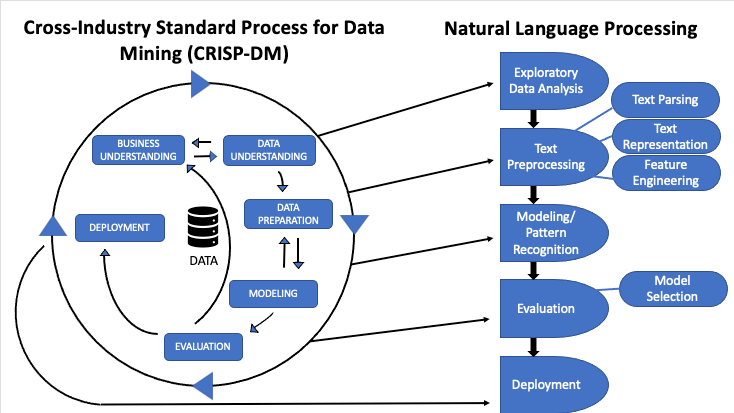
\includegraphics[width=1.0\textwidth]{nlp_workflow_cycle.png}
    \captionof{figure}{Quy trình Dự án NLP Tinh gọn: Một chu trình lặp đi lặp lại từ việc xác định bài toán đến triển khai và giám sát.}
    \label{fig:nlp_workflow_cycle}
\end{center}

\subsection{Vòng lặp 0: Xác định Bài toán và Thiết lập Đường cơ sở (Baseline)}
\label{ssec:workflow_step0}
Đây là bước quan trọng nhất, quyết định sự thành bại của toàn bộ dự án.

\subsubsection{1. Hiểu rõ Mục tiêu (Problem Framing)}
\begin{itemize}
    \item \textbf{Câu hỏi cần trả lời:} Chúng ta đang cố gắng giải quyết vấn đề kinh doanh/nghiên cứu nào? Tác động mong muốn là gì? (Ví dụ: "giảm 30\% thời gian phản hồi của nhân viên hỗ trợ", "tự động phân loại 80\% tin tức đầu vào").
    \item \textbf{Xác định Input và Output:} Đầu vào của mô hình là gì (văn bản thô, bình luận, email)? Đầu ra mong muốn là gì (một nhãn, một đoạn văn bản tóm tắt, một câu trả lời)?
    \item \textbf{Định hình bài toán NLP:} Ánh xạ vấn đề kinh doanh thành một bài toán NLP cụ thể. Ví dụ: "Giảm thời gian phản hồi" $\rightarrow$ "Xây dựng mô hình phân loại email để tự động định tuyến đến đúng phòng ban".
\end{itemize}

\subsubsection{2. Định nghĩa Metric Thành công}
\begin{itemize}
    \item \textbf{Metric Máy học (Offline):} Chọn các metric kỹ thuật để đánh giá mô hình trong quá trình phát triển (ví dụ: F1-score, Accuracy, BLEU). Metric này phải phản ánh được mục tiêu kinh doanh.
    \item \textbf{Metric Kinh doanh (Online):} Xác định cách bạn sẽ đo lường tác động thực tế của mô hình sau khi triển khai (ví dụ: tỷ lệ click, thời gian giải quyết ticket, mức độ hài lòng của khách hàng).
\end{itemize}

\subsubsection{3. Thiết lập một Đường cơ sở (Baseline) Đơn giản}
\begin{tcolorbox}[
    title=Lời khuyên quan trọng: Bắt đầu một cách "ngu ngốc",
    colback=yellow!10!white, colframe=yellow!50!black, fonttitle=\bfseries
]
Đừng bao giờ bắt đầu một dự án bằng việc xây dựng một mô hình Transformer phức tạp. Hãy bắt đầu với giải pháp đơn giản nhất có thể. Một baseline tốt không chỉ cho bạn một điểm để so sánh, mà còn có thể đủ tốt để giải quyết 80\% vấn đề với 20\% công sức.
\end{tcolorbox}
\begin{itemize}
    \item \textbf{Các ý tưởng cho Baseline:}
        \begin{itemize}
            \item \textbf{Không dùng ML:} Một hệ thống dựa trên từ khóa hoặc biểu thức chính quy (regex).
            \item \textbf{Mô hình Thống kê kinh điển:} Sử dụng `TF-IDF` kết hợp với `Logistic Regression` hoặc `Naive Bayes`. Các thư viện như `Scikit-learn` giúp việc này trở nên cực kỳ nhanh chóng.
            \item \textbf{Mô hình Zero-shot:} Sử dụng API của một LLM lớn (như GPT-4) với một prompt zero-shot. Đây là một baseline rất mạnh mẽ trong kỷ nguyên hiện đại.
        \end{itemize}
\end{itemize}

Baseline này sẽ là thước đo để bạn biết liệu những nỗ lực phức tạp hơn của mình có thực sự mang lại giá trị hay không.

\subsection{Vòng lặp 1: Phát triển Mô hình (Model Development)}
\label{ssec:workflow_step1}
Đây là vòng lặp cốt lõi của việc xây dựng và cải tiến mô hình.

\subsubsection{4. Thu thập và Chuẩn bị Dữ liệu}
Đây thường là phần tốn nhiều thời gian nhất.
\begin{itemize}
    \item \textbf{Thu thập (Collection):} Lấy dữ liệu từ các nguồn (cơ sở dữ liệu, API, web scraping).
    \item \textbf{Làm sạch (Cleaning):} Xử lý các vấn đề như mã hóa ký tự, loại bỏ các thẻ HTML, chuẩn hóa văn bản.
    \item \textbf{Gán nhãn (Labeling):} Nếu là bài toán có giám sát, đây là bước cực kỳ quan trọng. Sử dụng các công cụ như `Label Studio` hoặc các kỹ thuật gán nhãn yếu (weak supervision).
    \item \textbf{Phân chia Dữ liệu (Splitting):} Chia dữ liệu thành các tập Huấn luyện (Train), Đánh giá (Validation/Dev), và Kiểm tra (Test). \textbf{Không bao giờ} được "nhìn" vào tập Test trong quá trình phát triển.
\end{itemize}

\subsubsection{5. Huấn luyện Mô hình}
\begin{itemize}
    \item \textbf{Lựa chọn Mô hình:} Dựa trên baseline và yêu cầu của bài toán, chọn một kiến trúc phù hợp (ví dụ: một mô hình từ Hugging Face Hub).
    \item \textbf{Huấn luyện/Fine-tuning:} Thực hiện quá trình huấn luyện.
    \item \textbf{Theo dõi Thí nghiệm (Experiment Tracking):} Sử dụng các công cụ như `Weights \& Biases` hoặc `MLflow` để ghi lại mọi thứ: phiên bản code, siêu tham số, metric, và các mô hình đã được huấn luyện. Việc này là tối quan trọng để đảm bảo tính tái lập (reproducibility) và so sánh các thử nghiệm.
\end{itemize}

\subsubsection{6. Phân tích Lỗi (Error Analysis)}
Đây là bước mà nhiều người bỏ qua, nhưng nó lại là chìa khóa để cải tiến mô hình một cách thông minh.
\begin{itemize}
    \item \textbf{Mục tiêu:} Không chỉ nhìn vào con số metric tổng thể (ví dụ: F1 = 85\%), mà phải hiểu \textbf{tại sao} mô hình lại sai ở 15\% còn lại.
    \item \textbf{Quy trình:}
        \begin{enumerate}
            \item Lấy một mẫu các dự đoán sai trên tập validation.
            \item Phân loại các lỗi này thành các nhóm. Ví dụ: "mô hình sai ở các câu bị phủ định", "mô hình nhầm lẫn giữa hai lớp A và B", "lỗi do dữ liệu gán nhãn sai".
            \item \textbf{Ưu tiên:} Tập trung nỗ lực vào việc giải quyết nhóm lỗi lớn nhất và có tác động nhất. Ví dụ, nếu mô hình thường sai ở các câu phủ định, bạn có thể cần thu thập thêm dữ liệu về loại câu này hoặc sử dụng kỹ thuật tăng cường dữ liệu.
        \end{enumerate}
\end{itemize}
Vòng lặp (Huấn luyện $\rightarrow$ Phân tích lỗi $\rightarrow$ Cải thiện dữ liệu/mô hình) được lặp lại cho đến khi mô hình đạt được hiệu năng mong muốn trên tập validation.

\subsection{Vòng lặp 2: Triển khai và Giám sát (Deployment \& Monitoring)}
\label{ssec:workflow_step2}
Một mô hình chỉ thực sự tạo ra giá trị khi nó được đưa vào sử dụng.

\subsubsection{7. Đóng gói và Triển khai (Deployment)}
\begin{itemize}
    \item \textbf{Tối ưu hóa:} Áp dụng các kỹ thuật như lượng tử hóa (quantization) hoặc chưng cất (distillation) để làm cho mô hình nhỏ hơn và nhanh hơn.
    \item \textbf{Đóng gói (Packaging):} Đóng gói mô hình và các thành phần phụ thuộc của nó vào một định dạng có thể triển khai, ví dụ như một container Docker.
    \item \textbf{Phục vụ (Serving):} Triển khai mô hình như một API endpoint (sử dụng các framework như `FastAPI` hoặc `BentoML`) để các ứng dụng khác có thể gọi đến.
\end{itemize}

\subsubsection{8. Giám sát và Bảo trì (Monitoring \& Maintenance)}
Công việc không kết thúc sau khi triển khai.
\begin{itemize}
    \item \textbf{Giám sát Hiệu năng:} Theo dõi các metric của mô hình trong môi trường thực tế.
    \item \textbf{Phát hiện Trôi dạt Dữ liệu (Data Drift):} Thế giới thực luôn thay đổi. Cách người dùng viết và các chủ đề họ quan tâm có thể thay đổi theo thời gian. Cần có cơ chế để phát hiện khi nào phân phối dữ liệu đầu vào thực tế bắt đầu khác biệt so với dữ liệu huấn luyện.
    \item \textbf{Thu thập Phản hồi và Huấn luyện lại:} Thiết lập một vòng lặp để thu thập các dự đoán sai từ môi trường production, gán nhãn lại chúng, và sử dụng chúng để định kỳ huấn luyện lại (re-train) mô hình afin d'améliorer sa performance au fil du temps.
\end{itemize}
Quy trình tinh gọn này đảm bảo rằng bạn luôn tập trung vào việc tạo ra giá trị, học hỏi từ dữ liệu và các lỗi sai, và xây dựng các hệ thống NLP mạnh mẽ và bền vững.
% % File: chapters_part1/chap1_linguistics.tex

\section{Nền tảng Ngôn ngữ học cho NLP}
\label{sec:nen_tang_ngon_ngu_hoc}

Trong kỷ nguyên của Học sâu, khi các mô hình Transformer khổng lồ dường như có thể "học" mọi thứ từ dữ liệu thô, một câu hỏi chính đáng được đặt ra: "Liệu kiến thức về Ngôn ngữ học có còn cần thiết?". Câu trả lời là một tiếng "Có" dứt khoát.

Mặc dù chúng ta không còn phải viết tay các bộ quy tắc ngữ pháp phức tạp, việc hiểu các cấu trúc và nguyên lý cơ bản của ngôn ngữ mang lại những lợi ích to lớn:
\begin{itemize}
    \item \textbf{Thiết kế tác vụ (Task Design):} Giúp chúng ta định hình các bài toán NLP một cách có ý nghĩa. Ví dụ, tại sao "Nhận dạng Thực thể Tên" (NER) lại là một bài toán quan trọng? Vì "thực thể" là một khái niệm ngữ nghĩa cơ bản.
    \item \textbf{Kỹ thuật đặc trưng (Feature Engineering):} Cung cấp ý tưởng cho các đặc trưng hữu ích, đặc biệt khi dữ liệu bị hạn chế.
    \item \textbf{Phân tích lỗi (Error Analysis):} Giúp chúng ta hiểu tại sao một mô hình thất bại. Liệu nó thất bại vì không hiểu được cấu trúc cú pháp phức tạp, hay vì không giải quyết được sự đa nghĩa của từ?
    \item \textbf{Đánh giá (Evaluation):} Giúp xây dựng các bộ dữ liệu đánh giá có thể kiểm tra các năng lực ngôn ngữ cụ thể của mô hình.
\end{itemize}

Mục này sẽ giới thiệu những khái niệm Ngôn ngữ học cốt lõi nhất, đóng vai trò là lăng kính để chúng ta nhìn vào các bài toán NLP trong suốt giáo trình này.

\subsection{Các cấp độ phân tích ngôn ngữ: Hình thái học, Cú pháp, Ngữ nghĩa, Ngữ dụng}
\label{ssec:cap_do_phan_tich}

Ngôn ngữ học thường phân tích ngôn ngữ theo một hệ thống các cấp độ, đi từ đơn vị nhỏ nhất đến ý nghĩa trong bối cảnh rộng lớn nhất. Đây là một khung khái niệm vô cùng hữu ích để phân loại các bài toán NLP.

\paragraph{1. Hình thái học (Morphology)}
Là nghiên cứu về cấu trúc bên trong của từ. Hình thái học xem xét cách các từ được tạo thành từ những đơn vị có nghĩa nhỏ hơn gọi là \textbf{hình vị (morphemes)}.
\begin{itemize}
    \item \textbf{Ví dụ (tiếng Anh):} Từ \textit{unhappiness} được cấu tạo từ 3 hình vị: tiền tố \textit{un-} (phủ định), gốc từ \textit{happi} (hạnh phúc), và hậu tố \textit{-ness} (danh từ hóa).
    \item \textbf{Ví dụ (tiếng Việt):} Tiếng Việt là một ngôn ngữ đơn lập (isolating language), nên cấu trúc hình thái không phức tạp như tiếng Anh. Tuy nhiên, khái niệm này vẫn có thể áp dụng cho các từ ghép như \textit{học sinh} (gồm hình vị \textit{học} và \textit{sinh}) hay \textit{nhà khoa học} (\textit{nhà-} + \textit{khoa học}).
    \item \textbf{Ứng dụng trong NLP:} Lemmatization (đưa từ về dạng gốc, ví dụ: "running" $\rightarrow$ "run"), Stemming (cắt bỏ hậu tố), Phân tích hình thái.
\end{itemize}

\paragraph{2. Cú pháp (Syntax)}
Là nghiên cứu về cách các từ kết hợp với nhau để tạo thành các cụm từ (phrases) và câu (sentences) đúng ngữ pháp. Cú pháp tập trung vào \textbf{quy tắc cấu trúc} của câu.
\begin{itemize}
    \item \textbf{Ví dụ:} Câu "Con mèo đuổi con chuột" là đúng cú pháp tiếng Việt. Câu *"Mèo con chuột con đuổi"* thì không, mặc dù các từ vẫn giữ nguyên. Cú pháp quy định trật tự từ và các mối quan hệ ngữ pháp.
    \item \textbf{Ứng dụng trong NLP:} Phân tích cú pháp (Parsing), Gán nhãn Từ loại (Part-of-Speech Tagging), Kiểm tra ngữ pháp (Grammar Checking).
\end{itemize}

\paragraph{3. Ngữ nghĩa (Semantics)}
Là nghiên cứu về \textbf{ý nghĩa} của từ, cụm từ và câu, độc lập với ngữ cảnh. Ngữ nghĩa trả lời câu hỏi "Câu này có nghĩa là gì?".
\begin{itemize}
    \item \textbf{Ví dụ:} Câu "Colorless green ideas sleep furiously" (Những ý tưởng xanh không màu ngủ một cách giận dữ) của Noam Chomsky là một câu đúng về mặt cú pháp nhưng vô nghĩa về mặt ngữ nghĩa.
    \item Thử thách lớn của ngữ nghĩa là \textbf{sự mơ hồ (ambiguity)}. Ví dụ, từ "đường" có thể là "con đường" hoặc "đường ăn". Câu "Tôi thấy người đàn ông trên ngọn đồi với chiếc kính thiên văn" có thể có nghĩa là tôi dùng kính để thấy anh ta, hoặc anh ta là người có chiếc kính.
    \item \textbf{Ứng dụng trong NLP:} Phân biệt ý của từ (Word Sense Disambiguation - WSD), Gán nhãn vai nghĩa (Semantic Role Labeling - SRL), Biểu diễn ý nghĩa câu.
\end{itemize}

\paragraph{4. Ngữ dụng (Pragmatics)}
Là nghiên cứu về cách ngữ cảnh ảnh hưởng đến việc diễn giải ý nghĩa. Ngữ dụng xem xét ý định của người nói và cách người nghe hiểu được ý định đó. Nó trả lời câu hỏi "Người nói \textbf{muốn} nói gì khi nói câu này?".
\begin{itemize}
    \item \textbf{Ví dụ:} Nếu ai đó nói "Ở đây nóng quá", về mặt ngữ nghĩa, đó là một câu trần thuật về nhiệt độ. Nhưng về mặt ngữ dụng, đó có thể là một lời yêu cầu "Làm ơn bật quạt/điều hòa lên".
    \item \textbf{Ứng dụng trong NLP:} Phân tích hội thoại (Discourse Analysis), Phân giải đồng tham chiếu (Coreference Resolution - xác định "anh ấy" trong một câu là đang chỉ đến ai), Nhận dạng hành động nói (Speech Act Recognition), các hệ thống đối thoại (Dialogue Systems).
\end{itemize}

Bốn cấp độ này tạo thành một chuỗi xử lý tự nhiên: từ nhận diện các đơn vị nhỏ nhất của từ (hình thái), đến cách chúng kết hợp thành câu (cú pháp), rồi ý nghĩa của câu đó (ngữ nghĩa), và cuối cùng là ý nghĩa trong một bối cảnh cụ thể (ngữ dụng).

\subsection{Ngữ pháp hình thức (Formal Grammars): Ngữ pháp phi ngữ cảnh (CFG)}
\label{ssec:cfg}

Để máy tính có thể "hiểu" được cú pháp, các nhà ngôn ngữ học và khoa học máy tính đã phát triển các hệ thống quy tắc toán học gọi là \textbf{Ngữ pháp hình thức}. Một trong những loại ngữ pháp hình thức quan trọng và phổ biến nhất trong NLP thời kỳ đầu là \textbf{Ngữ pháp phi ngữ cảnh (Context-Free Grammar - CFG)}.

\begin{definition}{Ngữ pháp phi ngữ cảnh (CFG)}{def:cfg}
    Một CFG là một bộ quy tắc sản sinh (production rules) được dùng để tạo ra các chuỗi trong một ngôn ngữ. Nó được gọi là "phi ngữ cảnh" vì các quy tắc có thể được áp dụng bất kể ngữ cảnh xung quanh các ký hiệu. Một CFG được định nghĩa bởi một bộ 4 thành phần $(N, \Sigma, P, S)$:
    \begin{itemize}
        \item $N$: một tập hữu hạn các \textbf{ký hiệu phi-kết thúc} (non-terminal symbols), thường là các loại cụm từ như \texttt{NP} (Cụm danh từ), \texttt{VP} (Cụm động từ).
        \item $\Sigma$: một tập hữu hạn các \textbf{ký hiệu kết thúc} (terminal symbols), chính là các từ trong từ vựng.
        \item $P$: một tập hữu hạn các \textbf{quy tắc sản sinh} (production rules), có dạng $A \rightarrow \alpha$, trong đó $A \in N$ và $\alpha$ là một chuỗi các ký hiệu trong $(N \cup \Sigma)^*$.
        \item $S$: \textbf{ký hiệu bắt đầu} (start symbol), thường là \texttt{S} (Sentence - Câu), $S \in N$.
    \end{itemize}
\end{definition}

\begin{example}{Một CFG đơn giản cho Tiếng Việt}{ex:cfg_vietnamese}
    Hãy xem xét một ngữ pháp rất nhỏ để tạo ra câu "con mèo đuổi con chuột":
    \begin{itemize}
        \item $N = \{ \texttt{S, NP, VP, Det, N, V} \}$
        \item $\Sigma = \{ \text{con, mèo, đuổi, chuột} \}$
        \item $S = \texttt{S}$
        \item $P$ là tập các quy tắc sau:
            \begin{enumerate}
                \item \texttt{S $\rightarrow$ NP VP} (Một câu được tạo thành từ một Cụm danh từ và một Cụm động từ)
                \item \texttt{NP $\rightarrow$ Det N} (Một cụm danh từ được tạo thành từ một Từ hạn định và một Danh từ)
                \item \texttt{VP $\rightarrow$ V NP} (Một cụm động từ được tạo thành từ một Động từ và một Cụm danh từ)
                \item \texttt{Det $\rightarrow$ con}
                \item \texttt{N $\rightarrow$ mèo | chuột} (Ký hiệu `|` có nghĩa là "hoặc")
                \item \texttt{V $\rightarrow$ đuổi}
            \end{enumerate}
    \end{itemize}
    Sử dụng các quy tắc này, chúng ta có thể "sản sinh" ra câu mong muốn, và quá trình này có thể được hình dung bằng một \textbf{cây cú pháp (parse tree)}.
\end{example}

CFG là nền tảng lý thuyết cho \textit{phân tích cú pháp thành phần}, một khái niệm chúng ta sẽ tìm hiểu ngay sau đây.

\subsection{Các lý thuyết cú pháp chính: Cú pháp thành phần (Constituency) và Cú pháp phụ thuộc (Dependency)}
\label{ssec:constituency_dependency}

Khi phân tích cấu trúc cú pháp của một câu, có hai cách tiếp cận chính, tương ứng với hai "trường phái" lớn trong ngôn ngữ học và NLP.

\paragraph{1. Cú pháp thành phần (Constituency Syntax)}
Cách tiếp cận này, vốn bắt nguồn trực tiếp từ CFG của Noam Chomsky \cite{chomsky1956three}, cho rằng câu được cấu tạo từ các \textbf{thành phần (constituents)} hay \textbf{cụm từ (phrases)} lồng vào nhau. Mỗi cụm từ là một đơn vị ngữ pháp hoạt động như một khối thống nhất.
\begin{itemize}
    \item \textbf{Ý tưởng cốt lõi:} Chia câu thành các cụm từ, rồi lại chia các cụm từ đó thành các cụm từ nhỏ hơn cho đến khi còn lại các từ riêng lẻ.
    \item \textbf{Biểu diễn:} Sử dụng \textbf{cây cú pháp thành phần (constituency parse tree)}. Các nút trong (internal nodes) của cây là tên các cụm từ (\texttt{NP, VP, PP}), và các nút lá (leaf nodes) là các từ của câu.
    \item \textbf{Ví dụ:} Với câu "Con mèo đuổi con chuột", cây thành phần sẽ trông như sau:
    
    \begin{center}
        \texttt{(S (NP (Det con) (N mèo)) (VP (V đuổi) (NP (Det con) (N chuột))))}
    \end{center}
    
    Cấu trúc này cho thấy rõ "con mèo" là một khối (Cụm danh từ - \texttt{NP}) và "đuổi con chuột" là một khối khác (Cụm động từ - \texttt{VP}).
\end{itemize}

\paragraph{2. Cú pháp phụ thuộc (Dependency Syntax)}
Cách tiếp cận này không tập trung vào các cụm từ, mà tập trung vào mối quan hệ \textbf{phụ thuộc ngữ pháp} giữa các từ riêng lẻ.
\begin{itemize}
    \item \textbf{Ý tưởng cốt lõi:} Mỗi từ trong câu, ngoại trừ một từ gốc (thường là động từ chính), sẽ phụ thuộc vào một từ khác. Mối quan hệ này là mối quan hệ bất đối xứng giữa một \textbf{từ quản lý (head/governor)} và một \textbf{từ phụ thuộc (dependent/modifier)}.
    \item \textbf{Biểu diễn:} Sử dụng \textbf{cây cú pháp phụ thuộc (dependency parse tree)}, thực chất là một đồ thị có hướng. Các nút là các từ, và các cạnh có nhãn là tên của mối quan hệ ngữ pháp (ví dụ: \texttt{nsubj} - chủ ngữ, \texttt{obj} - tân ngữ, \texttt{det} - từ hạn định).
    \item \textbf{Ví dụ:} Với câu "Con mèo đuổi con chuột", đồ thị phụ thuộc sẽ có các quan hệ:
    
    \begin{itemize}
        \item \texttt{đuổi} là gốc (root) của câu.
        \item \texttt{mèo} là chủ ngữ (\texttt{nsubj}) của \texttt{đuổi}.
        \item \texttt{chuột} là tân ngữ (\texttt{obj}) của \texttt{đuổi}.
        \item \texttt{con} (thứ nhất) là từ hạn định (\texttt{det}) của \texttt{mèo}.
        \item \texttt{con} (thứ hai) là từ hạn định (\texttt{det}) của \texttt{chuột}.
    \end{itemize}
\end{itemize}

\begin{tcolorbox}[
    title=So sánh Cú pháp Thành phần và Phụ thuộc,
    colback=blue!5!white,
    colframe=blue!50!black,
    fonttitle=\bfseries
]
\begin{tabular}{p{0.45\linewidth} | p{0.45\linewidth}}
    \textbf{Cú pháp Thành phần} & \textbf{Cú pháp Phụ thuộc} \\
    \hline
    Tập trung vào các \textbf{cụm từ} và cấu trúc lồng nhau. & Tập trung vào \textbf{mối quan hệ giữa các từ}. \\
    \hline
    Cung cấp thông tin cấu trúc rõ ràng về các khối ngữ pháp. & Cung cấp thông tin rõ ràng về quan hệ chức năng (ai làm gì ai). \\
    \hline
    Phù hợp hơn cho các ngôn ngữ có trật tự từ cố định (như tiếng Anh). & Linh hoạt hơn với các ngôn ngữ có trật tự từ tự do. \\
    \hline
    Phổ biến trong ngôn ngữ học lý thuyết và các hệ thống NLP thế hệ cũ. & Rất phổ biến trong các công cụ NLP hiện đại (ví dụ: spaCy, Stanza) do tính hữu ích cho các tác vụ ngữ nghĩa và tốc độ phân tích nhanh hơn. \\
\end{tabular}
\end{tcolorbox}

Việc hiểu cả hai trường phái này rất quan trọng, vì chúng cung cấp những góc nhìn bổ trợ cho nhau về cấu trúc của ngôn ngữ và là nền tảng cho nhiều bài toán NLP cốt lõi mà chúng ta sẽ khám phá trong các chương tiếp theo.
% % !TEX root = ../main.tex
% File: chapters_part1/chap1_3.tex
% Nội dung cho Phần 1.3: Các Bài toán Cốt lõi trong NLP

\section{Các Bài toán Cốt lõi trong NLP}
\label{sec:bai_toan_cot_loi}

Sau khi đã có nền tảng về các cấp độ phân tích ngôn ngữ, chúng ta sẽ chính thức ánh xạ chúng vào các bài toán (tasks) cụ thể trong NLP. Việc hiểu rõ các bài toán này là cực kỳ quan trọng, vì chúng là những "viên gạch" cơ bản để xây dựng nên các ứng dụng NLP phức tạp hơn. Các bài toán này thường được nhóm lại theo cấp độ phân tích, từ từ, đến câu, và cuối cùng là các ứng dụng hoàn chỉnh.

\subsection{Phân tích cấp độ từ}
\label{ssec:phan_tich_tu}

Đây là nhóm các bài toán cơ bản nhất, xử lý và gán thông tin cho từng từ (token) riêng lẻ trong văn bản. Kết quả của các bài toán này thường là đầu vào cho các tác vụ phức tạp hơn.

\paragraph{Gán nhãn Từ loại (Part-of-Speech - POS Tagging)}
Là quá trình gán một nhãn từ loại (danh từ, động từ, tính từ, v.v.) cho mỗi từ trong một câu, dựa vào định nghĩa và ngữ cảnh của nó.
\begin{itemize}
    \item \textbf{Mục tiêu:} Giải quyết sự mơ hồ của từ. Ví dụ, từ "câu" trong "câu cá" là động từ, nhưng trong "câu văn" lại là danh từ.
    \item \textbf{Ví dụ đầu vào:} `Tôi thích đọc sách.`
    \item \textbf{Ví dụ đầu ra:} `Tôi/P thích/V đọc/V sách/N ./CH` (P: Đại từ, V: Động từ, N: Danh từ, CH: Dấu câu).
    \item \textbf{Tầm quan trọng:} Là một bước tiền xử lý nền tảng cho rất nhiều bài toán khác như phân tích cú pháp, nhận dạng thực thể, trích xuất thông tin.
\end{itemize}

\paragraph{Đưa từ về dạng gốc (Lemmatization và Stemming)}
Cả hai kỹ thuật này đều nhằm mục đích quy chuẩn hóa các dạng biến thể của một từ về một dạng chung.
\begin{itemize}
    \item \textbf{Stemming (Rút gọn về gốc từ):} Một phương pháp đơn giản, dựa trên quy tắc để cắt bỏ các hậu tố của từ. Nó nhanh nhưng đôi khi không chính xác về mặt ngôn ngữ.
        \begin{itemize}
            \item \textbf{Ví dụ (tiếng Anh):} "studies", "studying" $\rightarrow$ "studi".
        \end{itemize}
    \item \textbf{Lemmatization (Đưa về dạng từ điển):} Một phương pháp phức tạp hơn, sử dụng từ điển và phân tích hình thái để đưa từ về dạng nguyên thể (lemma) của nó.
        \begin{itemize}
            \item \textbf{Ví dụ (tiếng Anh):} "studies", "studying" $\rightarrow$ "study"; "better" $\rightarrow$ "good".
            \item \textbf{Ví dụ (tiếng Việt):} "đi học", "đi làm" có thể được chuẩn hóa về động từ "đi".
        \end{itemize}
    \item \textbf{Lựa chọn:} Lemmatization thường được ưu tiên hơn vì kết quả có ý nghĩa ngôn ngữ học, tuy nhiên nó chậm hơn và đòi hỏi nhiều tài nguyên hơn Stemming.
\end{itemize}

\paragraph{Phân tích Hình thái học (Morphological Analysis)}
Là bài toán phân tích một từ thành các hình vị (morphemes) cấu tạo nên nó. Bài toán này đặc biệt quan trọng đối với các ngôn ngữ chắp dính (agglutinative languages) như tiếng Thổ Nhĩ Kỳ, Phần Lan, nơi một từ có thể chứa rất nhiều thông tin ngữ pháp.
\begin{itemize}
    \item \textbf{Ví dụ (tiếng Anh):} `unhappiness` $\rightarrow$ `un-` (phủ định) + `happy` (gốc) + `-ness` (danh từ hóa).
    \item \textbf{Tầm quan trọng:} Giúp các mô hình hiểu được cấu trúc bên trong của từ, đặc biệt hữu ích khi gặp các từ hiếm hoặc chưa từng thấy (Out-of-Vocabulary - OOV).
\end{itemize}

\subsection{Phân tích cấp độ câu}
\label{ssec:phan_tich_cau}

Sau khi đã xử lý các từ riêng lẻ, bước tiếp theo là hiểu cách chúng kết hợp với nhau để tạo thành một câu có cấu trúc.

\paragraph{Phân tích cú pháp (Parsing)}
Đây là bài toán xác định cấu trúc ngữ pháp của một câu. Như đã đề cập ở mục \ref{ssec:constituency_dependency}, có hai loại phân tích cú pháp chính:
\begin{itemize}
    \item \textbf{Phân tích cú pháp Thành phần (Constituency Parsing):}
        \begin{itemize}
            \item \textbf{Mục tiêu:} Xây dựng một cây cú pháp thành phần, nhóm các từ thành các cụm từ có cấp bậc.
            \item \textbf{Đầu ra:} Một cấu trúc cây lồng nhau, ví dụ: \texttt{(S (NP (N Tôi)) (VP (V thích) (NP (N sách))))}.
        \end{itemize}
    \item \textbf{Phân tích cú pháp Phụ thuộc (Dependency Parsing):}
        \begin{itemize}
            \item \textbf{Mục tiêu:} Xác định các mối quan hệ phụ thuộc (ai làm gì ai, cái gì bổ nghĩa cho cái gì) giữa các từ.
            \item \textbf{Đầu ra:} Một tập các cặp (từ quản lý, quan hệ, từ phụ thuộc), ví dụ: \texttt{(thích, nsubj, Tôi)}, \texttt{(thích, obj, sách)}.
        \end{itemize}
\end{itemize}
Phân tích cú pháp là một trong những bài toán lâu đời và thách thức nhất trong NLP, là chìa khóa để "hiểu sâu" cấu trúc của một câu.

\subsection{Phân tích ngữ nghĩa}
\label{ssec:phan_tich_ngu_nghia}

Vượt ra ngoài cấu trúc, các bài toán ở cấp độ này cố gắng nắm bắt \textbf{ý nghĩa} của văn bản.

\paragraph{Nhận dạng Thực thể Tên (Named Entity Recognition - NER)}
Là bài toán tìm và phân loại các thực thể có tên trong văn bản thành các danh mục được định trước như Tên người (PER), Tổ chức (ORG), Địa điểm (LOC), Ngày tháng (DATE), v.v.
\begin{itemize}
    \item \textbf{Ví dụ đầu vào:} `Apple được thành lập bởi Steve Jobs tại Cupertino vào năm 1976.`
    \item \textbf{Ví dụ đầu ra:} `[Apple/ORG] được thành lập bởi [Steve Jobs/PER] tại [Cupertino/LOC] vào năm [1976/DATE].`
    \item \textbf{Tầm quan trọng:} Một tác vụ nền tảng cho việc trích xuất thông tin, xây dựng đồ thị tri thức và hệ thống hỏi đáp.
\end{itemize}

\paragraph{Phân biệt Ý của Từ (Word Sense Disambiguation - WSD)}
Là bài toán xác định xem một từ đa nghĩa đang được sử dụng với ý nghĩa nào trong một ngữ cảnh cụ thể.
\begin{itemize}
    \item \textbf{Ví dụ:} Trong câu "Ngân hàng nhà nước vừa hạ lãi suất", từ "ngân hàng" có nghĩa là một tổ chức tài chính, chứ không phải "bờ sông" (bờ, bank).
    \item \textbf{Thách thức:} Đây là một bài toán rất khó và lâu đời. Tuy nhiên, sự ra đời của các mô hình ngôn ngữ dựa trên ngữ cảnh (contextualized embeddings) như BERT đã ngầm giải quyết một phần lớn bài toán này.
\end{itemize}

\paragraph{Gán nhãn Vai nghĩa (Semantic Role Labeling - SRL)}
Là bài toán xác định "ai đã làm gì, cho ai, ở đâu, khi nào, và như thế nào" xung quanh một động từ chính (vị ngữ) trong câu.
\begin{itemize}
    \item \textbf{Mục tiêu:} Phân tích cấu trúc sự kiện (event structure) của câu.
    \item \textbf{Ví dụ đầu vào:} `Hôm qua, An đã tặng Hoa một cuốn sách ở thư viện.`
    \item \textbf{Vị ngữ:} `tặng`
    \item \textbf{Ví dụ đầu ra:}
        \begin{itemize}
            \item \texttt{AGENT} (Tác nhân): `An`
            \item \texttt{THEME} (Đối thể): `một cuốn sách`
            \item \texttt{RECIPIENT} (Người nhận): `Hoa`
            \item \texttt{TIME} (Thời gian): `Hôm qua`
            \item \texttt{LOCATION} (Địa điểm): `ở thư viện`
        \end{itemize}
    \item \textbf{Tầm quan trọng:} Giúp biến đổi văn bản phi cấu trúc thành thông tin có cấu trúc, rất hữu ích cho các hệ thống hỏi đáp và tóm tắt.
\end{itemize}

\paragraph{Trích xuất Quan hệ (Relation Extraction)}
Là bài toán xác định các mối quan hệ ngữ nghĩa giữa các thực thể đã được nhận dạng trong văn bản.
\begin{itemize}
    \item \textbf{Mục tiêu:} Xây dựng các bộ ba (triples) có dạng `(Thực thể 1, Quan hệ, Thực thể 2)`.
    \item \textbf{Ví dụ đầu vào:} `Apple được thành lập bởi Steve Jobs.`
    \item \textbf{Thực thể đã nhận dạng:} `[Apple/ORG]`, `[Steve Jobs/PER]`
    \item \textbf{Ví dụ đầu ra:} `(Steve Jobs, FounderOf, Apple)`
    \item \textbf{Tầm quan trọng:} Là bước cốt lõi để tự động xây dựng và bổ sung các cơ sở tri thức và đồ thị tri thức từ văn bản.
\end{itemize}

\subsection{Các bài toán Ứng dụng}
\label{ssec:bai_toan_ung_dung}

Đây là nhóm các bài toán ở cấp độ cao nhất, thường kết hợp kết quả từ nhiều bài toán cốt lõi ở trên để tạo ra các sản phẩm hữu ích cho người dùng cuối.

\begin{example}{Tổng quan các bài toán ứng dụng phổ biến}{ex:ung_dung_pho_bien}
    \begin{itemize}
        \item \textbf{Phân loại văn bản (Text Classification):} Gán một hoặc nhiều nhãn cho một đoạn văn bản. Đây là một trong những bài toán phổ biến nhất.
            \begin{itemize}
                \item \textit{Ví dụ:} Phân tích cảm xúc (Tích cực/Tiêu cực/Trung tính), Phân loại chủ đề tin tức (Thể thao/Chính trị/Giải trí), Phát hiện spam.
            \end{itemize}
        \item \textbf{Dịch máy (Machine Translation - MT):} Tự động dịch văn bản từ ngôn ngữ nguồn sang ngôn ngữ đích.
            \begin{itemize}
                \item \textit{Ví dụ:} Google Translate.
            \end{itemize}
        \item \textbf{Tóm tắt văn bản (Text Summarization):} Tạo ra một phiên bản ngắn gọn, súc tích nhưng vẫn chứa đựng những thông tin quan trọng nhất của một văn bản dài.
            \begin{itemize}
                \item \textit{Ví dụ:} Tóm tắt một bài báo dài thành 3 gạch đầu dòng chính.
            \end{itemize}
        \item \textbf{Hỏi đáp (Question Answering - QA):} Cung cấp một câu trả lời chính xác cho một câu hỏi do người dùng đặt ra.
            \begin{itemize}
                \item \textit{Ví dụ:} Tìm kiếm câu trả lời trong một đoạn văn bản cho trước (Extractive QA) hoặc tự sinh ra câu trả lời (Generative QA).
            \end{itemize}
        \item \textbf{Hệ thống Đối thoại (Dialogue Systems / Chatbots):} Xây dựng các tác tử (agents) có khả năng trò chuyện với con người một cách tự nhiên.
            \begin{itemize}
                \item \textit{Ví dụ:} Chatbot hỗ trợ khách hàng, trợ lý ảo.
            \end{itemize}
            \item \textbf{Suy luận Ngôn ngữ Tự nhiên (Natural Language Inference - NLI):} Xác định mối quan hệ logic (kéo theo, mâu thuẫn, hoặc trung lập) giữa một cặp câu (tiền đề và giả thuyết).
            \begin{itemize}
                \item \textit{Ví dụ:} Tiền đề: "Một người đàn ông đang chơi guitar." Giả thuyết: "Có người đang tạo ra âm nhạc." $\rightarrow$ Mối quan hệ: Kéo theo (Entailment).
            \end{itemize}
    \end{itemize}
\end{example}

Bản đồ các bài toán này cho thấy một lộ trình rõ ràng trong việc xử lý ngôn ngữ: từ việc hiểu các thành phần nhỏ nhất, đến việc lắp ráp chúng thành cấu trúc có ý nghĩa, và cuối cùng là sử dụng sự hiểu biết đó để thực hiện các nhiệm vụ phức tạp, mang lại giá trị thực tiễn. Trong các chương sau, chúng ta sẽ lần lượt tìm hiểu các mô hình và kỹ thuật để giải quyết từng bài toán này.
% % !TEX root = ../../main.tex
% File: part2/chapters1/chap1_4.tex

\section{Kỹ thuật Tăng cường Dữ liệu (Data Augmentation)}
\label{sec:data_augmentation}

\begin{tcolorbox}[
    title=Vấn đề: "Cơn đói" Dữ liệu,
    colback=red!5!white, colframe=red!75!black, fonttitle=\bfseries
]
Các mô hình học sâu, đặc biệt là các mô hình Transformer lớn, rất "đói" dữ liệu. Khi được fine-tune trên một bộ dữ liệu nhỏ, chúng có nguy cơ cao bị \textbf{quá khớp (overfitting)} -- tức là chúng "học thuộc lòng" các ví dụ trong tập huấn luyện thay vì học quy luật tổng quát, dẫn đến hiệu năng kém trên dữ liệu mới.
\end{tcolorbox}

\textbf{Tăng cường Dữ liệu (Data Augmentation)} là quá trình tạo ra các mẫu dữ liệu huấn luyện mới, "giả" nhưng hợp lý, từ các mẫu dữ liệu hiện có. Mục tiêu là làm tăng kích thước và sự đa dạng của bộ dữ liệu huấn luyện, giúp mô hình trở nên mạnh mẽ hơn (more robust) và có khả năng tổng quát hóa tốt hơn.

Điều quan trọng là các phép biến đổi phải \textbf{giữ nguyên nhãn (label-preserving)}. Ví dụ, nếu bạn thay đổi một câu có cảm xúc "Tích cực", câu mới được tạo ra cũng phải giữ nguyên cảm xúc "Tích cực".

Chúng ta sẽ khám phá một số kỹ thuật tăng cường dữ liệu phổ biến, từ đơn giản đến phức tạp.

\subsection{EDA: Các Phép toán Thay thế Đơn giản}
\label{ssec:eda}
EDA (Easy Data Augmentation - Wei \& Zou, 2019) là một bộ bốn kỹ thuật đơn giản nhưng lại hiệu quả một cách đáng ngạc nhiên.

\begin{itemize}
    \item \textbf{Synonym Replacement (SR) - Thay thế bằng Từ đồng nghĩa:}
        \begin{itemize}
            \item \textbf{Cơ chế:} Chọn ngẫu nhiên $n$ từ trong câu (không phải là stop words) và thay thế mỗi từ bằng một từ đồng nghĩa của nó, thường được lấy từ một kho từ vựng như WordNet.
            \item \textbf{Ví dụ:} "Bộ phim này rất \textbf{tuyệt vời} và \textbf{hấp dẫn}." $\rightarrow$ "Bộ phim này rất \textbf{xuất sắc} và \textbf{lôi cuốn}."
        \end{itemize}
    \item \textbf{Random Insertion (RI) - Chèn ngẫu nhiên:}
        \begin{itemize}
            \item \textbf{Cơ chế:} Tìm các từ đồng nghĩa của một vài từ ngẫu nhiên trong câu, sau đó chèn các từ đồng nghĩa đó vào các vị trí ngẫu nhiên trong câu.
            \item \textbf{Ví dụ:} "Bộ phim này rất tuyệt vời." $\rightarrow$ "Bộ phim \textbf{xuất sắc} này rất tuyệt vời."
        \end{itemize}
    \item \textbf{Random Swap (RS) - Hoán đổi ngẫu nhiên:}
        \begin{itemize}
            \item \textbf{Cơ chế:} Chọn ngẫu nhiên hai từ trong câu và hoán đổi vị trí của chúng.
            \item \textbf{Ví dụ:} "Bộ phim \textbf{này} rất \textbf{tuyệt vời}." $\rightarrow$ "Bộ phim \textbf{tuyệt vời} rất \textbf{này}."
        \end{itemize}
    \item \textbf{Random Deletion (RD) - Xóa ngẫu nhiên:}
        \begin{itemize}
            \item \textbf{Cơ chế:} Xóa ngẫu nhiên mỗi từ trong câu với một xác suất $p$ nào đó.
            \item \textbf{Ví dụ:} "Bộ phim này rất tuyệt vời và hấp dẫn." $\rightarrow$ "Bộ phim này tuyệt vời và hấp dẫn."
        \end{itemize}
\end{itemize}
\textbf{Lưu ý:} Các kỹ thuật EDA có thể tạo ra các câu không tự nhiên hoặc sai ngữ pháp (đặc biệt là RS và RI). Tuy nhiên, việc đưa một ít "nhiễu" này vào quá trình huấn luyện đôi khi lại giúp mô hình trở nên mạnh mẽ hơn. Chúng rất dễ triển khai và là một điểm khởi đầu tốt.

\subsection{Back-Translation: Tận dụng Sức mạnh của Dịch máy}
\label{ssec:back_translation}
Đây là một trong những kỹ thuật tăng cường dữ liệu chất lượng cao và phổ biến nhất.

\subsubsection{Trực giác cốt lõi}
Nếu chúng ta dịch một câu từ ngôn ngữ A sang ngôn ngữ B, rồi lại dịch ngược kết quả từ B trở lại A, chúng ta thường sẽ nhận được một câu có cùng ý nghĩa với câu gốc, nhưng được diễn đạt bằng các từ ngữ và cấu trúc câu khác.

\begin{tcolorbox}[
    title=Quy trình Back-Translation,
    colback=blue!5!white, colframe=blue!75!black, fonttitle=\bfseries
]
Câu gốc (Tiếng Việt) $\xrightarrow{\text{Dịch máy (Vi } \rightarrow \text{ En)}}$ Câu trung gian (Tiếng Anh) $\xrightarrow{\text{Dịch máy (En } \rightarrow \text{ Vi)}}$ Câu mới (Tiếng Việt)
\end{tcolorbox}

\begin{example}{Minh họa Back-Translation}{ex:back_translation_example}
    \begin{itemize}
        \item \textbf{Câu gốc (Vi):} "Tôi nghĩ rằng đây là một ý tưởng cực kỳ thông minh."
        \item \textbf{Dịch sang Anh:} "I think that this is an extremely intelligent idea."
        \item \textbf{Dịch ngược về Việt:} "Tôi cho rằng đây là một ý tưởng vô cùng thông minh."
    \end{itemize}
    Câu mới được tạo ra có cùng nhãn với câu gốc nhưng lại là một mẫu dữ liệu huấn luyện mới, giúp mô hình học cách khái quát hóa qua các cách diễn đạt khác nhau.
\end{example}

\subsubsection{Ưu điểm và Nhược điểm}
\begin{itemize}
    \item \textbf{Ưu điểm:}
        \begin{itemize}
            \item Thường tạo ra các câu có chất lượng ngữ pháp và ngữ nghĩa cao hơn nhiều so với các phương pháp EDA.
            \item Có khả năng tạo ra sự đa dạng lớn về cả từ vựng và cấu trúc câu.
        \end{itemize}
    \item \textbf{Nhược điểm:}
        \begin{itemize}
            \item Yêu cầu phải có các mô hình dịch máy chất lượng cao.
            \item Chi phí tính toán cao hơn vì phải gọi đến các mô hình dịch.
            \item Có nguy cơ ý nghĩa bị thay đổi ("lost in translation") nếu các mô hình dịch không đủ tốt.
        \end{itemize}
\end{itemize}

\subsection{Tăng cường Dữ liệu dựa trên LLM}
\label{ssec:llm_based_augmentation}
Với sự ra đời của các LLM mạnh mẽ, chúng ta có thể thực hiện các phép tăng cường dữ liệu tinh vi hơn nhiều.

\subsubsection{Diễn giải lại (Paraphrasing)}
Đây là một phiên bản nâng cao của Back-Translation. Thay vì đi qua một ngôn ngữ khác, chúng ta có thể yêu cầu trực tiếp một LLM:
\begin{tcolorbox}[colback=gray!5!white, colframe=gray!50!black, sharp corners]
\textbf{Prompt:} \\
Hãy viết lại câu sau đây theo 5 cách khác nhau, nhưng vẫn giữ nguyên ý nghĩa cốt lõi. \\
Câu gốc: "Sản phẩm này có chất lượng tuyệt vời so với giá tiền."
\end{tcolorbox}
LLM có thể sinh ra các phiên bản như: "Chất lượng của sản phẩm này vượt xa mong đợi so với mức giá.", "Đây là một món hời, chất lượng rất tốt.", v.v.

\subsubsection{Tạo dữ liệu theo ngữ cảnh}
Chúng ta có thể yêu cầu LLM tạo ra các ví dụ phù hợp với một kịch bản cụ thể, đặc biệt hữu ích để xử lý các "trường hợp rìa" (edge cases) mà mô hình thường làm sai.

\begin{example}{Tạo dữ liệu cho các trường hợp phủ định}{ex:llm_augmentation_negation}
    Giả sử phân tích lỗi cho thấy mô hình phân tích cảm xúc của chúng ta thường sai ở các câu có yếu tố phủ định. Chúng ta có thể dùng prompt:
    \begin{tcolorbox}[colback=gray!5!white, colframe=gray!50!black, sharp corners]
    \textbf{Prompt:} \\
    Dưới đây là một câu có cảm xúc Tích cực. Hãy viết lại nó để biến nó thành một câu có cảm xúc Tiêu cực bằng cách sử dụng các từ ngữ phủ định hoặc mỉa mai, nhưng vẫn giữ chủ đề chính.

    \textbf{Câu gốc (Tích cực):} "Dịch vụ khách hàng của họ rất nhanh và hiệu quả."

    \textbf{Câu mới (Tiêu cực):}
    \end{tcolorbox}
    \textbf{Đầu ra có thể có của LLM:} `"Đừng mong đợi dịch vụ khách hàng của họ sẽ nhanh và hiệu quả."` hoặc `"Nhanh và hiệu quả' không phải là những từ tôi sẽ dùng để mô tả dịch vụ khách hàng của họ."`
\end{example}
Cách tiếp cận này cho phép chúng ta tạo ra dữ liệu một cách có chủ đích để vá các "điểm yếu" cụ thể của mô hình.

\subsection{Lựa chọn Kỹ thuật Tăng cường}
\begin{itemize}
    \item \textbf{Bắt đầu đơn giản:} Luôn bắt đầu với EDA. Nó nhanh, miễn phí và có thể mang lại những cải thiện bất ngờ.
    \item \textbf{Khi cần chất lượng cao:} Back-Translation là một lựa chọn mạnh mẽ nếu bạn có quyền truy cập vào các API dịch tốt.
    \item \textbf{Khi cần sự kiểm soát và tinh vi:} Tận dụng LLM để diễn giải lại hoặc tạo ra dữ liệu cho các trường hợp cụ thể là hướng đi hiện đại và mạnh mẽ nhất.
    \item \textbf{Thận trọng:} Không phải lúc nào tăng cường dữ liệu cũng giúp ích. Nếu các mẫu dữ liệu mới được tạo ra có chất lượng thấp hoặc làm thay đổi nhãn, chúng có thể làm hại mô hình. Luôn đánh giá hiệu năng trên một tập validation riêng biệt để kiểm tra xem việc tăng cường có thực sự hiệu quả hay không.
\end{itemize}
% % !TEX root = ../main.tex
% File: chapters_part1/chap1_5.tex
% Nội dung cho Phần 1.5: Đạo đức và Trách nhiệm trong NLP

\section{Đạo đức và Trách nhiệm trong NLP (Ethics \& Responsible AI)}
\label{sec:dao_duc_trach_nhiem}

Khi các mô hình NLP ngày càng trở nên mạnh mẽ và được tích hợp sâu rộng vào xã hội -- từ việc quyết định hồ sơ xin việc, duyệt đơn vay vốn, đến việc định hình dư luận -- thì trách nhiệm của người tạo ra chúng cũng ngày càng lớn. Một mô hình NLP không chỉ là một công trình kỹ thuật; nó là một tác nhân có thể gây ra những ảnh hưởng thực tế, cả tích cực và tiêu cực, đến cuộc sống con người.

Do đó, việc xem xét các khía cạnh về đạo đức và xây dựng AI có trách nhiệm không phải là một lựa chọn, mà là một \textbf{yêu cầu bắt buộc} đối với bất kỳ ai làm việc trong lĩnh vực này. Mục này sẽ thảo luận về những thách thức và phương pháp tiếp cận chính.

\subsection{Các loại Thiên kiến (Bias) trong Dữ liệu và Mô hình}
\label{ssec:thien_kien_bias}

Thiên kiến là một trong những vấn đề đạo đức phổ biến và nguy hiểm nhất trong NLP. Mô hình học máy không tự "suy nghĩ" ra thiên kiến; chúng học và khuếch đại những thiên kiến đã tồn tại sẵn trong dữ liệu mà chúng được huấn luyện.

\begin{tcolorbox}[
    title={Nguyên tắc cốt lõi: ``Rác vào, Rác ra''},
    colback=red!5!white,
    colframe=red!75!black,
    fonttitle=\bfseries
]
Mô hình NLP là tấm gương phản chiếu dữ liệu huấn luyện. Nếu dữ liệu chứa đựng các định kiến về giới tính, chủng tộc, hay văn hóa của xã hội, mô hình sẽ học và tái tạo lại những định kiến đó, thường với một quy mô lớn hơn rất nhiều. Đây còn được gọi là nguyên tắc "Garbage In, Garbage Out", nhưng trong bối cảnh đạo đức, nó trở thành "Bias In, Bias Out".
\end{tcolorbox}

Một số loại thiên kiến phổ biến bao gồm:
\begin{itemize}
    \item \textbf{Thiên kiến xã hội (Societal Bias):} Phản ánh các định kiến và khuôn mẫu trong xã hội.
        \begin{itemize}
            \item \textbf{Ví dụ:} Các mô hình word embedding cổ điển khi được huấn luyện trên kho văn bản lớn thường học được các liên kết như: "đàn ông" gần với "lập trình viên", trong khi "phụ nữ" gần với "nội trợ". Một hệ thống tuyển dụng dựa trên mô hình này có thể sẽ tự động đánh giá thấp hồ sơ của ứng viên nữ cho vị trí kỹ thuật.
        \end{itemize}
    \item \textbf{Thiên kiến chọn mẫu (Selection Bias):} Xảy ra khi dữ liệu được thu thập không đại diện cho thực tế.
        \begin{itemize}
            \item \textbf{Ví dụ:} Xây dựng một mô hình phân tích cảm xúc chỉ dựa trên các bài đánh giá sản phẩm công nghệ có thể sẽ hoạt động kém khi áp dụng cho các bình luận về phim ảnh, vì cách dùng từ và biểu đạt cảm xúc là khác nhau.
        \end{itemize}
    \item \textbf{Thiên kiến từ mô hình (Model Bias):} Bản thân kiến trúc hoặc quá trình tối ưu hóa của mô hình có thể vô tình tạo ra hoặc khuếch đại thiên kiến.
        \begin{itemize}
            \item \textbf{Ví dụ:} Một mô hình được tối ưu hóa để đạt độ chính xác cao nhất trên một bộ dữ liệu mất cân bằng (99\% email là không spam, 1\% là spam) có thể học được một chiến lược đơn giản là "luôn dự đoán không spam" để đạt độ chính xác 99\%, nhưng hoàn toàn vô dụng trong thực tế.
        \end{itemize}
\end{itemize}

\subsection{Tính Công bằng, Minh bạch và Diễn giải được (Fairness, Transparency, Interpretability)}
\label{ssec:fairness_transparency_interpretability}

Để đối phó với thiên kiến và xây dựng các hệ thống đáng tin cậy, ba khái niệm sau đây là trụ cột chính:

\paragraph{Tính Công bằng (Fairness)}
Là nỗ lực đảm bảo rằng các quyết định của mô hình không gây bất lợi một cách có hệ thống cho các nhóm nhân khẩu học nhất định (dựa trên giới tính, chủng tộc, tuổi tác, v.v.). Đây là một khái niệm phức tạp, không có một định nghĩa toán học duy nhất nào là hoàn hảo cho mọi trường hợp.

\paragraph{Tính Minh bạch (Transparency)}
Đề cập đến khả năng hiểu được cơ chế hoạt động bên trong của mô hình. Các mô hình đơn giản như Hồi quy Logistic có tính minh bạch cao (chúng ta có thể xem các trọng số). Tuy nhiên, các mô hình ngôn ngữ lớn (LLMs) là những "hộp đen" (black boxes) gần như không thể minh bạch.

\paragraph{Tính Diễn giải được (Interpretability / Explainable AI - XAI)}
Khi không thể đạt được sự minh bạch hoàn toàn, chúng ta hướng tới tính diễn giải được: khả năng giải thích \textit{tại sao} mô hình lại đưa ra một dự đoán cụ thể. Hai kỹ thuật phổ biến để làm điều này là:
\begin{itemize}
    \item \textbf{LIME (Local Interpretable Model-agnostic Explanations):} Giải thích một dự đoán riêng lẻ bằng cách xây dựng một mô hình đơn giản, có thể diễn giải được (như một mô hình tuyến tính) chỉ hoạt động tốt "tại vùng lân cận" của dự đoán đó. Nó trả lời câu hỏi: "Những từ nào trong câu này đã đóng góp nhiều nhất vào quyết định của mô hình?".
    \item \textbf{SHAP (SHapley Additive exPlanations):} Dựa trên lý thuyết trò chơi, SHAP tính toán sự đóng góp của mỗi đặc trưng (mỗi từ) vào đầu ra của mô hình một cách công bằng và nhất quán. Nó cung cấp một nền tảng lý thuyết vững chắc hơn cho việc diễn giải.
\end{itemize}

\subsection{Quyền riêng tư và An toàn Dữ liệu (Federated Learning, Differential Privacy)}
\label{ssec:quyen_rieng_tu}

Các mô hình NLP được huấn luyện trên lượng dữ liệu khổng lồ, thường được thu thập từ người dùng. Điều này làm dấy lên những lo ngại nghiêm trọng về quyền riêng tư.

\paragraph{Vấn đề:} Các mô hình, đặc biệt là LLMs, có thể "ghi nhớ" và vô tình tiết lộ thông tin nhận dạng cá nhân (Personally Identifiable Information - PII) có trong dữ liệu huấn luyện, chẳng hạn như số điện thoại, địa chỉ email, hoặc thông tin y tế nhạy cảm.

Hai kỹ thuật tiên tiến để giải quyết vấn đề này là:
\begin{itemize}
    \item \textbf{Học Liên kết (Federated Learning - FL):} Thay vì thu thập tất cả dữ liệu về một máy chủ trung tâm để huấn luyện, phương pháp này "gửi" mô hình đến các thiết bị của người dùng (ví dụ: điện thoại di động). Mô hình được huấn luyện cục bộ trên dữ liệu của người dùng, sau đó chỉ có các cập nhật (gradients) của mô hình được gửi về máy chủ để tổng hợp. Dữ liệu thô không bao giờ rời khỏi thiết bị của người dùng.
    \item \textbf{Bảo toàn riêng tư vi phân (Differential Privacy - DP):} Cung cấp một sự đảm bảo toán học mạnh mẽ về quyền riêng tư. Ý tưởng cốt lõi là thêm một lượng nhiễu (noise) được kiểm soát cẩn thận vào dữ liệu hoặc kết quả của thuật toán, sao cho việc thêm hay bớt dữ liệu của một cá nhân bất kỳ trong tập dữ liệu gần như không làm thay đổi kết quả cuối cùng. Điều này khiến cho việc xác định thông tin của một cá nhân cụ thể trở nên bất khả thi.
\end{itemize}

\subsection{Mối nguy về Thông tin Sai lệch và Lạm dụng}
\label{ssec:thong_tin_sai_lech}

Sự ra đời của các mô hình sinh ngôn ngữ (Generative Models) có khả năng tạo ra văn bản chất lượng cao, mạch lạc và thuyết phục đã mở ra một "chiếc hộp Pandora" về các nguy cơ lạm dụng.
\begin{itemize}
    \item \textbf{Thông tin sai lệch (Misinformation \& Disinformation):} Các mô hình có thể được sử dụng để tạo ra hàng loạt tin tức giả, các bài đăng trên mạng xã hội, các bài đánh giá sản phẩm giả mạo với quy mô và tốc độ chưa từng có, gây ảnh hưởng đến dư luận, chính trị và xã hội.
    \item \textbf{Lừa đảo và Tấn công mạng (Scams \& Phishing):} Tự động tạo ra các email lừa đảo tinh vi, được cá nhân hóa cao, khiến người dùng khó phân biệt hơn nhiều.
    \item \textbf{Sáng tạo nội dung độc hại (Generation of Harmful Content):} Các mô hình có thể bị lợi dụng để tạo ra ngôn từ thù địch, tuyên truyền cực đoan, hoặc nội dung quấy rối.
\end{itemize}

Việc giải quyết những vấn đề này không chỉ nằm ở khía cạnh kỹ thuật (ví dụ: xây dựng các mô hình phát hiện văn bản do AI tạo ra) mà còn đòi hỏi sự chung tay của toàn xã hội, bao gồm việc xây dựng các chính sách quản lý, nâng cao nhận thức và giáo dục kỹ năng số cho cộng đồng.

Kết thúc chương đầu tiên này, hy vọng bạn không chỉ nắm được "NLP là gì?" mà còn nhận thức được trách nhiệm to lớn đi kèm với sức mạnh của nó.

\subsection{Tính Bền vững và Tấn công Giả mạo (Robustness \& Adversarial Attacks)}
\label{ssec:robustness_adversarial_attacks}

Ngoài các vấn đề về thiên kiến và quyền riêng tư, một khía cạnh quan trọng khác của AI có trách nhiệm là đảm bảo mô hình hoạt động một cách đáng tin cậy trong thế giới thực. Một mô hình có thể đạt độ chính xác 99\% trên bộ dữ liệu kiểm thử sạch (clean test set), nhưng lại có thể thất bại thảm hại khi đối mặt với dữ liệu thực tế vốn luôn nhiễu và không hoàn hảo. Đây là bài toán về \textbf{tính bền vững (robustness)}.

Đáng lo ngại hơn, các mô hình NLP, đặc biệt là các mô hình học sâu, lại rất dễ bị tổn thương trước các \textbf{tấn công giả mạo (adversarial attacks)} -- những thay đổi nhỏ, thường không thể nhận biết bởi con người, được thiết kế một cách có chủ đích để đánh lừa mô hình.

\begin{tcolorbox}[
    title={Sự Mong manh của các Mô hình "Thông minh"},
    colback=blue!5!white,
    colframe=blue!75!black,
    fonttitle=\bfseries
]
Một tấn công giả mạo có thể thay đổi dự đoán của mô hình một cách hoàn toàn. Ví dụ, một mô hình phân tích cảm xúc có thể phân loại câu "Bộ phim này thật tuyệt vời" là \texttt{TÍCH CỰC}. Kẻ tấn công có thể chỉ cần thêm một vài ký tự vô hình hoặc thay một từ bằng một từ đồng nghĩa được chọn lọc cẩn thận để biến nó thành câu "Bộ phim này thật \textit{xuất chúng}", và mô hình đột ngột thay đổi dự đoán thành \texttt{TIÊU CỰC}. Đối với con người, ý nghĩa không thay đổi, nhưng đối với mô hình, kết quả đã bị đảo ngược.
\end{tcolorbox}

Các kỹ thuật tấn công phổ biến bao gồm:
\begin{itemize}
    \item \textbf{Tấn công cấp độ ký tự (Character-level):} Thay thế, chèn, hoặc xóa các ký tự. Ví dụ: thay chữ "o" bằng số "0", hoặc chèn các ký tự không thể in ra (non-printable characters). \textit{DeepWordBug} \cite{gao2018black} hay \textit{HotFlip} \cite{ebrahimi2017hotflip} thực hiện các kỹ thuật này.
    \item \textbf{Tấn công cấp độ từ (Word-level):} Thay thế các từ bằng từ đồng nghĩa của chúng. Thách thức ở đây là tìm ra từ đồng nghĩa nào sẽ đánh lừa mô hình mà không làm thay đổi ý nghĩa của câu đối với con người. \textit{TextFooler} \cite{jin2020bert} là một ví dụ kinh điển, nó xác định các từ quan trọng nhất trong câu và thay thế chúng một cách chiến lược.
    \item \textbf{Tấn công cấp độ câu (Sentence-level):} Diễn giải (paraphrase) lại toàn bộ câu để giữ nguyên ý nghĩa nhưng sử dụng cấu trúc và từ vựng khác, nhằm mục đích tìm ra một phiên bản mà mô hình không thể hiểu đúng.
\end{itemize}

Việc một mô hình dễ bị tấn công cho thấy nó không thực sự "hiểu" ngôn ngữ, mà chỉ đang dựa vào các quy luật và mẫu thống kê bề mặt. Để phòng thủ, các nhà nghiên cứu đã phát triển nhiều kỹ thuật, trong đó phổ biến nhất là:
\begin{itemize}
    \item \textbf{Huấn luyện Giả mạo (Adversarial Training):} Đây là phương pháp phòng thủ trực tiếp và hiệu quả nhất. Trong quá trình huấn luyện, chúng ta chủ động tạo ra các mẫu dữ liệu giả mạo và đưa chúng vào tập huấn luyện cùng với nhãn đúng. Điều này giống như việc "tiêm vắc-xin" cho mô hình, giúp nó học cách miễn nhiễm với các loại tấn công tương tự trong tương lai.
    \item \textbf{Phát hiện Dữ liệu Giả mạo (Adversarial Detection):} Xây dựng một mô hình phụ để xác định xem một đầu vào có phải là một mẫu giả mạo hay không trước khi đưa nó vào mô hình chính.
\end{itemize}

Việc xây dựng các mô hình bền vững không chỉ là một thách thức kỹ thuật mà còn là một yêu cầu về mặt đạo đức, đặc biệt khi NLP được triển khai trong các hệ thống có tính rủi ro cao như lọc nội dung độc hại, phát hiện tin giả, hay các ứng dụng an ninh mạng.

\bigskip
\hrule
\bigskip

\begin{center}
    \textbf{\Large KẾT THÚC CHƯƠNG 1}
\end{center}

\textit{Kết thúc chương mở đầu này, bạn đã có trong tay một tấm bản đồ toàn diện về thế giới NLP. Chúng ta đã cùng nhau định nghĩa lĩnh vực, khám phá các nền tảng ngôn ngữ học và toán học, vạch ra các bài toán cốt lõi, và quan trọng nhất, thiết lập một la bàn đạo đức cho hành trình phía trước. Giờ đây, khi đã hiểu rõ "cái gì" và "tại sao", đã đến lúc chúng ta đi sâu vào kỹ thuật đầu tiên: làm thế nào để biến văn bản thành các con số có thể tính toán được. Chương tiếp theo sẽ giới thiệu các phương pháp biểu diễn văn bản kinh điển, khởi đầu cho kỷ nguyên thống kê của NLP.}

% \chapter{CÁC KIẾN TRÚC MẠNG NƠ-RON KINH ĐIỂN}
\label{chap:deep_learning_architectures}

Chào mừng bạn đến với kỷ nguyên học sâu của NLP. Trong chương 2, chúng ta đã thấy các mô hình thống kê như N-gram có thể nắm bắt các phụ thuộc cục bộ, nhưng lại bất lực trước các mối quan hệ tầm xa. Cuộc cách mạng word embedding đã cho chúng ta các vector từ mang đầy ngữ nghĩa, nhưng làm thế nào để kết hợp chúng lại nhằm hiểu được ý nghĩa của cả một câu hay một đoạn văn?

Chương này sẽ giới thiệu các kiến trúc mạng nơ-ron nền tảng được thiết kế đặc biệt để xử lý dữ liệu dạng chuỗi như ngôn ngữ tự nhiên. Những kiến trúc này không chỉ đơn thuần "nhìn" vào các từ một cách riêng lẻ, mà còn có khả năng "ghi nhớ" và "lý luận" dựa trên thông tin đã xử lý trước đó, cho phép chúng nắm bắt được ngữ cảnh và các phụ thuộc phức tạp trong câu.
% % !TEX root = ../main.tex
% File: chapters_part1/chap2_1.tex
% Nội dung cho Phần 2.1: Biểu diễn Dựa trên Tần suất


\section{Biểu diễn Dựa trên Tần suất (Bag-of-Words, TF-IDF)}
\label{sec:frequency_representation}

Phương pháp tiếp cận đầu tiên và trực quan nhất để biểu diễn văn bản là dựa trên một giả định đơn giản: \textit{tần suất xuất hiện của các từ trong một tài liệu phản ánh nội dung chính của tài liệu đó}. Hai kỹ thuật tiêu biểu nhất cho trường phái này là Bag-of-Words và TF-IDF.

\subsection{Túi từ (Bag-of-Words - BoW)}
\label{ssec:bow}

\subsubsection{Tư duy cốt lõi}

Mô hình Bag-of-Words (BoW) là một trong những phương pháp biểu diễn văn bản đơn giản nhưng mạnh mẽ nhất. Tư duy cốt lõi của nó là \textbf{hoàn toàn bỏ qua trật tự từ và cấu trúc ngữ pháp, và chỉ quan tâm đến việc từ nào xuất hiện và xuất hiện bao nhiêu lần} trong một tài liệu.

Hãy tưởng tượng bạn lấy tất cả các từ trong một câu, cho chúng vào một chiếc túi, xáo trộn lên và rồi thống kê số lượng của từng từ. Chiếc túi đó chính là "Bag-of-Words". Kết quả của quá trình này là một vector số, trong đó mỗi chiều của vector tương ứng với một từ trong từ vựng và giá trị của chiều đó là tần suất xuất hiện của từ.

\subsubsection{Quy trình xây dựng mô hình BoW}
Để xây dựng biểu diễn BoW cho một tập hợp các tài liệu (corpus), chúng ta thực hiện ba bước chính:

\paragraph{Bước 1: Tokenization (Tách từ)}
Tách các câu trong tài liệu thành các từ riêng lẻ (tokens). Đây là bước cơ bản để có được đơn vị cần đếm. Ví dụ, câu "NLP rất thú vị" được tách thành `['NLP', 'rất', 'thú vị']`.

\paragraph{Bước 2: Xây dựng Từ vựng (Vocabulary Building)}
Tập hợp tất cả các từ độc nhất từ toàn bộ kho tài liệu để tạo ra một bộ từ vựng. Thứ tự của các từ trong từ vựng này sẽ quyết định thứ tự các chiều trong vector biểu diễn cuối cùng.
Ví dụ, nếu từ vựng là `['NLP', 'rất', 'thú vị', 'học', 'thích']`, thì từ 'NLP' sẽ tương ứng với chiều thứ nhất, 'rất' với chiều thứ hai, v.v.

\paragraph{Bước 3: Vector hóa (Vectorization)}
Đối với mỗi tài liệu, tạo ra một vector có số chiều bằng kích thước của từ vựng. Với mỗi từ trong từ vựng, ta đếm số lần nó xuất hiện trong tài liệu và điền con số đó vào chiều tương ứng của vector. Nếu một từ trong từ vựng không xuất hiện trong tài liệu, giá trị ở chiều đó sẽ là 0.

\begin{example}{Xây dựng biểu diễn BoW}{ex:bow_example}
    Giả sử chúng ta có một kho tài liệu nhỏ (corpus) gồm 2 câu:
    \begin{itemize}
        \item \textbf{Câu 1:} "Tôi thích học NLP."
        \item \textbf{Câu 2:} "Học NLP rất rất thú vị."
    \end{itemize}
    
    \textbf{Bước 1 \& 2: Tokenization và Xây dựng Từ vựng} \\
    Sau khi tách từ và loại bỏ dấu câu, chúng ta có các từ: `tôi`, `thích`, `học`, `nlp`, `học`, `nlp`, `rất`, `thú vị`.
    Từ vựng độc nhất (sắp xếp theo alphabet) sẽ là:
    \texttt{['học', 'NLP', 'rất', 'thích', 'thú vị', 'tôi']}
    Kích thước từ vựng là 6.
    
    \textbf{Bước 3: Vector hóa} \\
    Bây giờ, chúng ta biểu diễn mỗi câu bằng một vector 6 chiều:
    \begin{itemize}
        \item \textbf{Câu 1:} "tôi thích học nlp"
            \begin{itemize}
                \item `học`: 1 lần
                \item `NLP`: 1 lần
                \item `rất`: 0 lần
                \item `thích`: 1 lần
                \item `thú vị`: 0 lần
                \item `tôi`: 1 lần
            \end{itemize}
            \(\rightarrow\) Vector biểu diễn: \textbf{[1, 1, 0, 1, 0, 1]}
        
        \item \textbf{Câu 2:} "học nlp rất rất thú vị"
            \begin{itemize}
                \item `học`: 1 lần
                \item `NLP`: 1 lần
                \item `rất`: 2 lần
                \item `thích`: 0 lần
                \item `thú vị`: 1 lần
                \item `tôi`: 0 lần
            \end{itemize}
            \(\rightarrow\) Vector biểu diễn: \textbf{[1, 1, 2, 0, 1, 0]}
    \end{itemize}
\end{example}
\subsubsection{Ưu điểm và Nhược điểm của BoW}
Mô hình BoW, mặc dù đơn giản, lại là nền tảng cho nhiều hệ thống phân loại văn bản kinh điển.
\begin{tcolorbox}[
    title=Đánh giá mô hình Bag-of-Words,
    colback=blue!5!white, colframe=blue!50!black, fonttitle=\bfseries,
    breakable
]
\textbf{Ưu điểm:}
\begin{itemize}
    \item \textbf{Đơn giản và trực quan:} Rất dễ hiểu và dễ triển khai.
    \item \textbf{Hiệu quả tính toán:} Việc tạo và sử dụng các vector BoW tương đối nhanh.
    \item \textbf{Hoạt động tốt cho các tác vụ phân loại chủ đề:} Nếu hai tài liệu có các bộ từ vựng tương tự nhau, chúng có khả năng cùng một chủ đề. BoW nắm bắt rất tốt điều này.
\end{itemize}
\textbf{Nhược điểm:}
\begin{itemize}
    \item \textbf{Mất thông tin về trật tự từ:} Câu "chó cắn người" và "người cắn chó" có cùng biểu diễn BoW, nhưng ý nghĩa hoàn toàn trái ngược. Đây là nhược điểm lớn nhất.
    \item \textbf{Không nắm bắt được ngữ nghĩa:} BoW không hiểu rằng "tốt" và "tuyệt vời" là những từ gần nghĩa. Đối với nó, đây là hai chiều hoàn toàn khác biệt trong không gian vector.
    \item \textbf{Vấn đề về kích thước từ vựng và độ thưa thớt (Sparsity):} Với một kho dữ liệu lớn, kích thước từ vựng có thể lên tới hàng trăm nghìn từ. Điều này tạo ra các vector có số chiều rất lớn, và hầu hết các giá trị trong vector đều là 0 (vì một tài liệu chỉ chứa một phần nhỏ của từ vựng). Các vector thưa thớt này gây khó khăn cho nhiều thuật toán học máy.
\end{itemize}
\end{tcolorbox}


\subsection{TF-IDF: Trọng số hóa tầm quan trọng của từ}
\label{ssec:tfidf}

Một trong những vấn đề của BoW là nó coi mọi từ có vai trò như nhau. Một từ xuất hiện nhiều lần (như "là", "thì", "của", "và" - gọi là các stop words) có thể lấn át các từ mang ý nghĩa quan trọng nhưng xuất hiện ít hơn. TF-IDF (Term Frequency - Inverse Document Frequency) \cite{sparck1972statistical} ra đời để giải quyết vấn đề này.

\subsubsection{Tư duy cốt lõi}

Tư duy của TF-IDF là: \textbf{Một từ càng quan trọng đối với một tài liệu nếu nó xuất hiện nhiều lần trong tài liệu đó (tính quan trọng cục bộ), nhưng lại xuất hiện ít trong các tài liệu khác của toàn bộ kho dữ liệu (tính độc nhất). }

TF-IDF tính toán một trọng số cho mỗi từ trong mỗi tài liệu, thay vì chỉ đếm tần suất. Trọng số này được cấu thành từ hai thành phần: TF và IDF.

\subsubsection{Các thành phần của TF-IDF}

\paragraph{Term Frequency (TF) - Tần suất của Từ}
TF đo lường tần suất xuất hiện của một từ $t$ trong một tài liệu $d$. Có nhiều cách tính TF, nhưng cách đơn giản nhất là đếm số lần xuất hiện.
$$ \text{TF}(t, d) = \text{số lần từ } t \text{ xuất hiện trong tài liệu } d $$
Để tránh việc các tài liệu dài có lợi thế, người ta thường chuẩn hóa TF, ví dụ bằng cách chia cho tổng số từ trong tài liệu.

\paragraph{Inverse Document Frequency (IDF) - Tần suất Nghịch của Tài liệu}
IDF đo lường mức độ "hiếm" hay "độc nhất" của một từ trên toàn bộ kho tài liệu. Nếu một từ xuất hiện trong rất nhiều tài liệu, IDF của nó sẽ thấp và ngược lại.
$$ \text{IDF}(t, D) = \log\left(\frac{N}{|\{d \in D : t \in d\}|}\right) $$
Trong đó:
\begin{itemize}
    \item $N$ là tổng số tài liệu trong kho dữ liệu $D$.
    \item $|\{d \in D : t \in d\}|$ là số tài liệu có chứa từ $t$.
    \item Logarit được dùng để "làm mịn" giá trị, tránh việc các từ cực hiếm có trọng số quá lớn. Để tránh chia cho 0, trong thực tế mẫu số thường được cộng thêm 1.
\end{itemize}

\paragraph{Trọng số TF-IDF}
Trọng số cuối cùng của từ $t$ trong tài liệu $d$ là tích của TF và IDF.

\begin{equation}
    \text{TF-IDF}(t, d, D) = \text{TF}(t, d) \times \text{IDF}(t, D)
    \label{eq:tfidf}
\end{equation}

\begin{example}{Tính toán trọng số TF-IDF}{ex:tfidf_example}
    Chúng ta tiếp tục với kho tài liệu ở ví dụ \ref{ex:bow_example}:
    \begin{itemize}
        \item \textbf{Câu 1 (d1):} "Tôi thích học NLP."
        \item \textbf{Câu 2 (d2):} "Học NLP rất rất thú vị."
        \item \textbf{Từ vựng:} `['học', 'NLP', 'rất', 'thích', 'thú vị', 'tôi']`
        \item \textbf{Tổng số tài liệu N = 2}
    \end{itemize}

    \textbf{1. Tính TF (dùng số đếm thô):}
    \begin{center}
    \begin{tabular}{|l|c|c|}
        \hline
        \textbf{Từ (t)} & \textbf{TF(t, d1)} & \textbf{TF(t, d2)} \\
        \hline
        `học` & 1 & 1 \\
        `NLP` & 1 & 1 \\
        `rất` & 0 & 2 \\
        `thích` & 1 & 0 \\
        `thú vị` & 0 & 1 \\
        `tôi` & 1 & 0 \\
        \hline
    \end{tabular}
    \end{center}

    \textbf{2. Tính IDF:}
    \begin{itemize}
        \item `học`: xuất hiện trong 2 tài liệu \(\rightarrow\) IDF = $\log(2/2) = 0$
        \item `NLP`: xuất hiện trong 2 tài liệu \(\rightarrow\) IDF = $\log(2/2) = 0$
        \item `rất`: xuất hiện trong 1 tài liệu \(\rightarrow\) IDF = $\log(2/1) \approx 0.693$
        \item `thích`: xuất hiện trong 1 tài liệu \(\rightarrow\) IDF = $\log(2/1) \approx 0.693$
        \item `thú vị`: xuất hiện trong 1 tài liệu \(\rightarrow\) IDF = $\log(2/1) \approx 0.693$
        \item `tôi`: xuất hiện trong 1 tài liệu \(\rightarrow\) IDF = $\log(2/1) \approx 0.693$
    \end{itemize}
    
    \textbf{3. Tính TF-IDF = TF * IDF:}
    \begin{center}
    \begin{tabular}{|l|c|c|}
        \hline
        \textbf{Từ (t)} & \textbf{TF-IDF(t, d1)} & \textbf{TF-IDF(t, d2)} \\
        \hline
        `học` & 1 * 0 = 0 & 1 * 0 = 0 \\
        `NLP` & 1 * 0 = 0 & 1 * 0 = 0 \\
        `rất` & 0 * 0.693 = 0 & 2 * 0.693 = 1.386 \\
        `thích` & 1 * 0.693 = 0.693 & 0 * 0.693 = 0 \\
        `thú vị` & 0 * 0.693 = 0 & 1 * 0.693 = 0.693 \\
        `tôi` & 1 * 0.693 = 0.693 & 0 * 0.693 = 0 \\
        \hline
    \end{tabular}
    \end{center}
    
    \textbf{Kết quả Vector TF-IDF:}
    \begin{itemize}
        \item \textbf{Câu 1 (d1):} `[0, 0, 0, 0.693, 0, 0.693]`
        \item \textbf{Câu 2 (d2):} `[0, 0, 1.386, 0, 0.693, 0]`
    \end{itemize}
    
    \textbf{Nhận xét quan trọng:} Các từ `học` và `NLP` xuất hiện trong cả hai câu, bị coi là "thông tin chung" và có trọng số TF-IDF bằng 0. Ngược lại, các từ `thích`, `tôi` trở thành đặc trưng của Câu 1, trong khi `rất`, `thú vị` là đặc trưng của Câu 2. Đây chính là sức mạnh của TF-IDF.
\end{example}

\subsubsection{Tổng kết về TF-IDF}
TF-IDF là một bước tiến lớn so với BoW. Nó vẫn giữ được sự đơn giản trong tính toán nhưng thông minh hơn trong việc trọng số hóa các từ. Nó đã và đang được sử dụng rộng rãi trong các hệ thống tìm kiếm thông tin (information retrieval) và phân loại văn bản.

Tuy nhiên, TF-IDF vẫn kế thừa các nhược điểm cố hữu của họ phương pháp dựa trên túi từ: nó vẫn \textbf{bỏ qua trật tự từ và không hiểu được ngữ nghĩa}. Những hạn chế này chính là động lực để cộng đồng NLP phát triển các phương pháp biểu diễn phức tạp và mạnh mẽ hơn, mà chúng ta sẽ khám phá trong phần tiếp theo: Word Embeddings.
% % !TEX root = ../main.tex
% File: chapters_part1/chap2_2.tex
% Nội dung cho Phần 2.2: Mô hình Ngôn ngữ Thống kê

\section{Mô hình Ngôn ngữ Thống kê (N-gram, Smoothing)}
\label{sec:statistical_lm}

Trong mục trước, chúng ta đã học cách biểu diễn văn bản như một "túi từ" không có trật tự. Bây giờ, chúng ta sẽ đưa trật tự từ trở lại và giới thiệu một trong những ý tưởng mạnh mẽ nhất của NLP thống kê: \textbf{Mô hình Ngôn ngữ (Language Model - LM)}.

\begin{definition}{Mô hình Ngôn ngữ (LM)}{def:lm}
    Một Mô hình Ngôn ngữ là một mô hình xác suất có khả năng gán một giá trị xác suất cho một chuỗi các từ bất kỳ. Nói cách khác, một LM có thể trả lời câu hỏi: "Xác suất để một chuỗi từ $W = w_1, w_2, \dots, w_n$ xuất hiện trong một ngôn ngữ là bao nhiêu?", ký hiệu là $P(W)$.
\end{definition}

Một LM tốt sẽ gán xác suất cao cho những câu "tự nhiên", đúng ngữ pháp (ví dụ: "tôi thích học NLP") và gán xác suất rất thấp cho những câu vô nghĩa, sai ngữ pháp (ví dụ: "thích tôi học NLP NLP").

\textbf{Ứng dụng của Mô hình Ngôn ngữ:}
LM là trái tim của rất nhiều ứng dụng NLP, đặc biệt là các ứng dụng sinh ngôn ngữ:
\begin{itemize}
    \item \textbf{Dịch máy:} Chọn câu dịch có xác suất cao nhất trong ngôn ngữ đích.
    \item \textbf{Nhận dạng giọng nói:} Phân biệt giữa hai câu phát âm gần giống nhau (ví dụ: "I saw a van" và "ice Havana") bằng cách chọn câu có xác suất ngôn ngữ cao hơn.
    \item \textbf{Kiểm tra chính tả và ngữ pháp:} Gợi ý sửa lỗi "I \underline{is} a student" thành "I \underline{am} a student" vì câu sau có xác suất cao hơn nhiều.
    \item \textbf{Gợi ý từ tiếp theo (Predictive Text):} Dự đoán từ có khả năng xuất hiện tiếp theo nhất dựa trên các từ đã gõ.
\end{itemize}

\subsection{Mô hình N-gram: Học từ Lịch sử Gần nhất}
\label{ssec:ngram}

\subsubsection{Thách thức của việc tính toán xác suất chuỗi}
Để tính xác suất của một chuỗi từ $P(W) = P(w_1, w_2, \dots, w_n)$, chúng ta có thể sử dụng quy tắc chuỗi (chain rule) trong xác suất:
$$ P(w_1, w_2, \dots, w_n) = P(w_1) \times P(w_2|w_1) \times P(w_3|w_1, w_2) \times \dots \times P(w_n|w_1, \dots, w_{n-1}) $$
$$ P(W) = \prod_{i=1}^{n} P(w_i | w_1, \dots, w_{i-1}) $$

Tuy nhiên, việc tính toán trực tiếp công thức này là \textbf{bất khả thi} trong thực tế. Để tính $P(w_n|w_1, \dots, w_{n-1})$, chúng ta cần phải thống kê được tần suất của chuỗi $w_1, \dots, w_{n-1}, w_n$ đã xuất hiện trong kho dữ liệu huấn luyện. Với các câu dài, chuỗi này gần như chắc chắn \textbf{chưa từng xuất hiện bao giờ}, dẫn đến vấn đề \textit{dữ liệu thưa thớt (sparsity)} nghiêm trọng.

\subsubsection{Giả định Markov và N-gram}
Để giải quyết vấn đề này, các mô hình N-gram đưa ra một giả định đơn giản hóa, gọi là \textbf{Giả định Markov (Markov Assumption)}:

\begin{tcolorbox}[
    title=Giả định Markov,
    colback=green!5!white, colframe=green!60!black, fonttitle=\bfseries
]
Xác suất của từ tiếp theo không phụ thuộc vào toàn bộ lịch sử các từ trước đó, mà chỉ phụ thuộc vào một vài từ đứng ngay trước nó. Cụ thể, nó chỉ phụ thuộc vào $N-1$ từ gần nhất.
\end{tcolorbox}

Dựa trên giả định này, xác suất của từ $w_i$ được xấp xỉ như sau:
$$ P(w_i | w_1, \dots, w_{i-1}) \approx P(w_i | w_{i-N+1}, \dots, w_{i-1}) $$

Một chuỗi gồm $N$ từ được gọi là một \textbf{N-gram}. Dựa trên giá trị của $N$, chúng ta có các mô hình cụ thể:
\begin{itemize}
    \item \textbf{Unigram (N=1):} Xác suất của một từ không phụ thuộc vào bất kỳ từ nào trước đó. $P(w_i|w_1, \dots, w_{i-1}) \approx P(w_i)$. Mô hình này tương đương với Bag-of-Words.
    \item \textbf{Bigram (N=2):} Xác suất của một từ chỉ phụ thuộc vào từ đứng ngay trước nó. $P(w_i|w_1, \dots, w_{i-1}) \approx P(w_i|w_{i-1})$.
    \item \textbf{Trigram (N=3):} Xác suất của một từ phụ thuộc vào hai từ đứng ngay trước nó. $P(w_i|w_1, \dots, w_{i-1}) \approx P(w_i|w_{i-2}, w_{i-1})$.
\end{itemize}

\subsubsection{Ước lượng xác suất N-gram}
Xác suất của một N-gram có thể được ước lượng dễ dàng từ một kho văn bản huấn luyện bằng phương pháp Ước lượng Hợp lý Cực đại (MLE):
$$ P(w_i | w_{i-N+1}, \dots, w_{i-1}) = \frac{\text{Count}(w_{i-N+1}, \dots, w_{i-1}, w_i)}{\text{Count}(w_{i-N+1}, \dots, w_{i-1})} $$
Nói cách khác, xác suất của một bigram $P(w_i|w_{i-1})$ là số lần chuỗi "$w_{i-1} w_i$" xuất hiện, chia cho số lần tiền tố "$w_{i-1}$" xuất hiện.

\begin{example}{Xây dựng và sử dụng mô hình Bigram}{ex:bigram_model}
    Giả sử chúng ta có một kho văn bản rất nhỏ sau khi đã thêm các ký hiệu bắt đầu (`<s>`) và kết thúc (`</s>`) câu:
    \begin{itemize}
        \item `<s> tôi thích học NLP </s>`
        \item `<s> tôi thích AI </s>`
        \item `<s> học NLP rất vui </s>`
    \end{itemize}

    \textbf{1. Đếm tần suất Bigram:}
    \begin{center}
    \begin{tabular}{|l|c||l|c|}
        \hline
        \textbf{Bigram} & \textbf{Count} & \textbf{Bigram} & \textbf{Count} \\
        \hline
        `(<s>, tôi)` & 2 & `(học, NLP)` & 2 \\
        `(tôi, thích)` & 2 & `(NLP, </s>)` & 1 \\
        `(thích, học)` & 1 & `(NLP, rất)` & 1 \\
        `(thích, AI)` & 1 & `(rất, vui)` & 1 \\
        `(AI, </s>)` & 1 & `(vui, </s>)` & 1 \\
        `(<s>, học)` & 1 & & \\
        \hline
    \end{tabular}
    \end{center}

    \textbf{2. Đếm tần suất Unigram (tiền tố):}
    `Count(<s>) = 3`, `Count(tôi) = 2`, `Count(thích) = 2`, `Count(học) = 2`, `Count(NLP) = 2`, ...

    \textbf{3. Tính xác suất Bigram:}
    \begin{itemize}
        \item $P(\text{tôi} | \text{<s>}) = \frac{\text{Count(<s>, tôi)}}{\text{Count(<s>)}} = \frac{2}{3}$
        \item $P(\text{học} | \text{thích}) = \frac{\text{Count(thích, học)}}{\text{Count(thích)}} = \frac{1}{2}$
        \item $P(\text{AI} | \text{thích}) = \frac{\text{Count(thích, AI)}}{\text{Count(thích)}} = \frac{1}{2}$
        \item $P(\text{rất} | \text{NLP}) = \frac{\text{Count(NLP, rất)}}{\text{Count(NLP)}} = \frac{1}{2}$
    \end{itemize}

    \textbf{4. Tính xác suất cho một câu mới:}
    Hãy tính xác suất của câu "tôi thích NLP":
    $P(\text{<s> tôi thích NLP </s>}) = P(\text{tôi}|\text{<s>}) \times P(\text{thích}|\text{tôi}) \times P(\text{NLP}|\text{thích}) \times P(\text{</s>}|\text{NLP})$

    Tuy nhiên, hãy nhìn vào bảng tần suất. Bigram `(thích, NLP)` chưa từng xuất hiện! `Count(thích, NLP) = 0`.
    Điều này dẫn đến $P(\text{NLP}|\text{thích}) = 0$.
    Và kết quả là $P(\text{<s> tôi thích NLP </s>}) = 0$.

    Mô hình của chúng ta đã gán xác suất bằng 0 cho một câu hoàn toàn hợp lý. Đây chính là \textbf{vấn đề xác suất zero}.
\end{example}

\subsection{Làm mịn (Smoothing): Giải quyết vấn đề Xác suất Zero}
\label{ssec:smoothing}

Vấn đề xác suất zero xảy ra vì kho văn bản huấn luyện của chúng ta luôn có giới hạn và không thể chứa tất cả các N-gram có thể có trong một ngôn ngữ. Việc gán xác suất bằng 0 cho một N-gram chưa từng thấy là rất nguy hiểm, vì nó sẽ khiến xác suất của cả câu bằng 0.

\textbf{Làm mịn (Smoothing)} là một tập hợp các kỹ thuật được thiết kế để "vay mượn" một phần khối lượng xác suất từ các N-gram đã thấy và phân phối lại nó cho các N-gram chưa từng thấy.

\subsubsection{Cộng Laplace (Laplace Add-One Smoothing)}
Đây là kỹ thuật làm mịn đơn giản nhất và trực quan nhất. Ý tưởng là: Hãy giả vờ rằng chúng ta đã thấy tất cả các N-gram có thể có ít nhất một lần.

\begin{definition}{Làm mịn cộng Laplace}{def:laplace}
    Khi tính toán xác suất, chúng ta cộng 1 vào tử số (số đếm N-gram) và cộng $V$ (kích thước từ vựng) vào mẫu số (số đếm tiền tố).
    $$ P_{\text{Laplace}}(w_i | w_{i-1}) = \frac{\text{Count}(w_{i-1}, w_i) + 1}{\text{Count}(w_{i-1}) + V} $$
\end{definition}

\begin{example}{Áp dụng làm mịn Laplace}{ex:laplace_example}
    Quay trở lại ví dụ Bigram. Giả sử từ vựng của chúng ta gồm 6 từ: `tôi, thích, học, NLP, AI, rất, vui` cộng với `<s>, </s>`, vậy $V=9$.
    Chúng ta muốn tính lại $P(\text{NLP}|\text{thích})$.
    \begin{itemize}
        \item `Count(thích, NLP) = 0`
        \item `Count(thích) = 2`
    \end{itemize}
    
    $$ P_{\text{Laplace}}(\text{NLP} | \text{thích}) = \frac{0 + 1}{2 + 9} = \frac{1}{11} $$
    
    Xác suất bây giờ đã khác 0! Tuy nhiên, hãy xem điều gì xảy ra với các xác suất khác:
    $$ P_{\text{Laplace}}(\text{học} | \text{thích}) = \frac{1 + 1}{2 + 9} = \frac{2}{11} $$
    
    \textbf{Vấn đề của Laplace Smoothing:} Nó hoạt động, nhưng nó thường "cho đi" quá nhiều khối lượng xác suất. Trong các từ vựng lớn, nó làm thay đổi đáng kể xác suất của các N-gram đã thấy, khiến mô hình kém chính xác hơn.
\end{example}

\subsubsection{Các kỹ thuật làm mịn tiên tiến hơn}
Do nhược điểm của Laplace, nhiều kỹ thuật phức tạp hơn đã được phát triển. Dưới đây là ý tưởng chính của một số phương pháp phổ biến:

\paragraph{Làm mịn Add-k (Add-k Smoothing)}
Một sự tổng quát hóa của Laplace, thay vì cộng 1, chúng ta cộng một hằng số nhỏ $k$ (ví dụ: $k=0.1$).
$$ P_{\text{Add-k}}(w_i | w_{i-1}) = \frac{\text{Count}(w_{i-1}, w_i) + k}{\text{Count}(w_{i-1}) + kV} $$
Điều này giúp giảm bớt việc "cho đi" quá nhiều xác suất, nhưng việc chọn $k$ tối ưu cũng là một thách thức.

\paragraph{Good-Turing Smoothing}
Ý tưởng cốt lõi là sử dụng số lượng các N-gram chỉ xuất hiện một lần (`Count=1`) để ước tính tổng xác suất của các N-gram chưa từng thấy (`Count=0`). Nó dựa trên một quan sát thông minh: tần suất của những thứ bạn chưa thấy có thể được ước tính bằng tần suất của những thứ bạn chỉ thấy một lần.

\paragraph{Kneser-Ney Smoothing}
Đây được coi là kỹ thuật làm mịn \textbf{hiện đại và hiệu quả nhất} cho các mô hình N-gram. Nó rất phức tạp nhưng ý tưởng chính là: xác suất của một N-gram chưa thấy không nên được tính dựa trên tần suất của tiền tố, mà nên dựa trên \textit{số lượng các ngữ cảnh khác nhau mà từ cuối cùng của N-gram đó đã xuất hiện}. Nó trả lời câu hỏi "Từ 'San Francisco' có khả năng đi sau từ 'I live in' như thế nào?". Kneser-Ney sẽ ưu tiên các từ như 'Francisco' (vốn thường đi sau các từ khác như 'San') hơn là các từ phổ biến nhưng ít đa dạng về ngữ cảnh.

\subsection{Tổng kết và Hạn chế của N-gram}
Mô hình N-gram là một công cụ mạnh mẽ, tương đối đơn giản và đã thống trị các ứng dụng NLP trong nhiều năm. Tuy nhiên, chúng có những hạn chế cố hữu:
\begin{itemize}
    \item \textbf{Vấn đề thưa thớt (Sparsity):} Mặc dù có các kỹ thuật làm mịn, vấn đề này vẫn tồn tại, đặc biệt với N > 3. Việc lưu trữ tất cả các N-gram cũng rất tốn bộ nhớ.
    \item \textbf{Không nắm bắt được phụ thuộc tầm xa:} Một mô hình trigram không thể nắm bắt được mối liên hệ giữa chủ ngữ và động từ trong câu "The man who I saw yesterday in the park \underline{is} my friend." Nó chỉ nhìn thấy "in the park \underline{is}" và sẽ gặp khó khăn.
    \item \textbf{Không có khái niệm về ngữ nghĩa:} Giống như BoW, N-gram không hiểu rằng "mèo" và "hổ" đều là động vật.
\end{itemize}

Những hạn chế này chính là động lực thúc đẩy sự ra đời của các mô hình dựa trên mạng nơ-ron và word embeddings, những chủ đề chúng ta sẽ khám phá trong phần tiếp theo của chương này và các chương sau.
% % !TEX root = ../main.tex
% File: chapters_part1/chap2_3.tex
% Nội dung cho Phần 2.3: Các thuật toán Học máy Thống kê

\section{Các thuật toán Học máy Thống kê}
\label{sec:statistical_ml_algos}

Sau khi đã biến đổi văn bản thành các vector số (sử dụng BoW hoặc TF-IDF), chúng ta đã sẵn sàng để "dạy" cho máy tính. Các thuật toán học máy thống kê là những công cụ cho phép chúng ta xây dựng các mô hình có khả năng học các mẫu (patterns) từ dữ liệu đã được gán nhãn, và sau đó sử dụng các mẫu đó để đưa ra dự đoán trên dữ liệu mới.

Mục này sẽ giới thiệu một số thuật toán kinh điển đã tạo nên xương sống của NLP trong kỷ nguyên thống kê. Chúng được chia thành hai nhóm chính: các mô hình cho bài toán \textbf{phân loại} và các mô hình cho bài toán \textbf{học chuỗi}.

\subsection{Các mô hình Phân loại (Classification Models)}
\label{ssec:classification_models}
Đây là nhóm các thuật toán dùng để giải quyết các bài toán phân loại văn bản, ví dụ như phân tích cảm xúc (tích cực/tiêu cực), phân loại chủ đề tin tức, phát hiện thư rác.

\subsubsection{Naive Bayes}
Naive Bayes là một trong những thuật toán phân loại đơn giản, nhanh và đáng ngạc nhiên là rất hiệu quả cho các tác vụ văn bản \cite{manning2008introduction}.

\paragraph{Trực giác cốt lõi}
Thuật toán này dựa trên \textbf{Định lý Bayes}. Để phân loại một tài liệu $d$ vào một lớp $c$ (ví dụ: `spam` hoặc `not-spam`), Naive Bayes tính toán xác suất của mỗi lớp khi biết tài liệu đó, $P(c|d)$, và chọn lớp có xác suất cao nhất.

Sử dụng định lý Bayes, ta có:
$$ P(c|d) = \frac{P(d|c) \cdot P(c)}{P(d)} $$
Trong đó:
\begin{itemize}
    \item $P(c|d)$: Xác suất hậu nghiệm (posterior) - xác suất của lớp $c$ khi biết tài liệu $d$. Đây là thứ chúng ta muốn tìm.
    \item $P(d|c)$: Xác suất khả năng (likelihood) - xác suất của tài liệu $d$ khi biết nó thuộc lớp $c$.
    \item $P(c)$: Xác suất tiên nghiệm (prior) - xác suất của lớp $c$ trong toàn bộ dữ liệu.
    \item $P(d)$: Xác suất của tài liệu $d$. Vì $P(d)$ là hằng số đối với tất cả các lớp, chúng ta có thể bỏ qua nó khi so sánh các lớp với nhau.
\end{itemize}
Do đó, việc tối đa hóa $P(c|d)$ tương đương với việc tối đa hóa $P(d|c) \cdot P(c)$.

\paragraph{Giả định "Ngây thơ" (The "Naive" Assumption)}
Để tính $P(d|c) = P(w_1, w_2, \dots, w_n | c)$, Naive Bayes đưa ra một giả định rất mạnh và "ngây thơ" (naive): \textbf{các từ (đặc trưng) trong tài liệu là độc lập có điều kiện với nhau khi biết lớp $c$}.
$$ P(d|c) = P(w_1, w_2, \dots, w_n | c) \approx \prod_{i=1}^{n} P(w_i | c) $$
Mặc dù giả định này rõ ràng là sai trong thực tế (trật tự từ và sự phụ thuộc giữa các từ là rất quan trọng), nó giúp việc tính toán trở nên cực kỳ đơn giản và hiệu quả.

\paragraph{Công thức cuối cùng}
Lớp $\hat{c}$ được dự đoán cho tài liệu $d$ là:
\begin{equation}
    \hat{c} = \underset{c \in C}{\arg\max} \left( P(c) \cdot \prod_{i=1}^{n} P(w_i | c) \right)
    \label{eq:naive_bayes}
\end{equation}
Trong thực tế, do tích của nhiều xác suất nhỏ có thể dẫn đến sai số làm tròn, người ta thường tính toán trên logarit:
$$ \hat{c} = \underset{c \in C}{\arg\max} \left( \log P(c) + \sum_{i=1}^{n} \log P(w_i | c) \right) $$
Các xác suất $P(c)$ và $P(w_i|c)$ được học từ tập dữ liệu huấn luyện bằng cách đếm tần suất và sử dụng kỹ thuật làm mịn (ví dụ: Laplace) để tránh xác suất zero.

\begin{tcolorbox}[
    title=Đánh giá Naive Bayes,
    colback=blue!5!white, colframe=blue!50!black, fonttitle=\bfseries
]
\textbf{Ưu điểm:}
\begin{itemize}
    \item \textbf{Cực kỳ nhanh:} Cả quá trình huấn luyện và dự đoán đều chỉ là các phép đếm và nhân/cộng, rất hiệu quả.
    \item \textbf{Cần ít dữ liệu huấn luyện:} Hoạt động tương đối tốt ngay cả với dữ liệu nhỏ.
    \item \textbf{Mô hình diễn giải được:} Có thể kiểm tra xác suất $P(w|c)$ để xem từ nào đóng góp nhiều nhất vào việc phân loại một lớp.
\end{itemize}
\textbf{Nhược điểm:}
\begin{itemize}
    \item \textbf{Giả định độc lập "ngây thơ":} Không thể nắm bắt mối quan hệ và trật tự từ, làm hạn chế hiệu năng ở các bài toán phức tạp.
\end{itemize}
\end{tcolorbox}


\subsubsection{Hồi quy Logistic (Logistic Regression)}
Hồi quy Logistic \cite{hosmer2013applied}, mặc dù tên gọi có chữ "hồi quy", lại là một thuật toán phân loại mạnh mẽ và được sử dụng cực kỳ rộng rãi. Nó thuộc nhóm các mô hình \textbf{phân biệt (discriminative models)}, trái ngược với Naive Bayes là một mô hình \textbf{sinh (generative model)}.

\paragraph{Trực giác cốt lõi}
Thay vì mô hình hóa $P(d|c)$ như Naive Bayes, Hồi quy Logistic mô hình hóa trực tiếp xác suất hậu nghiệm $P(c|d)$. Nó học một \textbf{ranh giới quyết định (decision boundary)} tuyến tính để phân tách các lớp trong không gian đặc trưng.

\begin{center}
    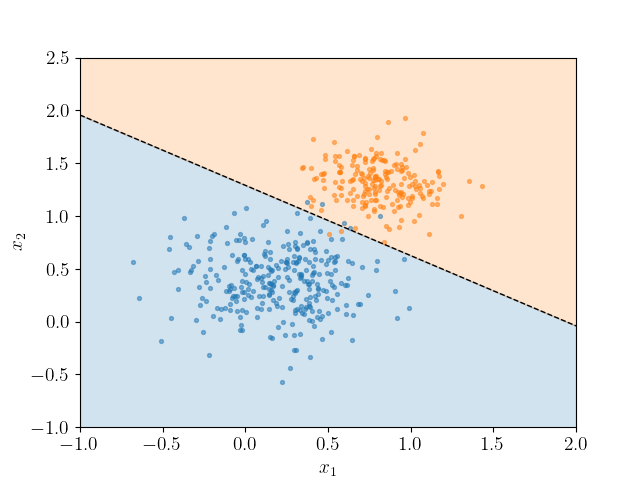
\includegraphics[width=0.7\textwidth]{logistic_regression_boundary.png}
    \captionof{figure}{Hồi quy Logistic học một đường thẳng (hoặc siêu phẳng trong không gian nhiều chiều) để phân chia dữ liệu thành các lớp.}
    \label{fig:logistic_regression_boundary}
\end{center}

\paragraph{Cơ chế hoạt động}
Cho một vector đầu vào $x$ (ví dụ, vector TF-IDF của tài liệu), mô hình thực hiện 2 bước:
\begin{enumerate}
    \item \textbf{Tính toán điểm số tuyến tính (Linear Score):} Mô hình tính một tổng có trọng số của các đặc trưng đầu vào. Mỗi đặc trưng $x_j$ (tương ứng với một từ trong từ vựng) có một trọng số $w_j$.
    $$ z = w_0 + w_1 x_1 + w_2 x_2 + \dots + w_m x_m = w^T x $$
    Trọng số $w_j$ có thể được diễn giải là: một giá trị dương lớn cho thấy sự hiện diện của từ $j$ làm tăng khả năng tài liệu thuộc lớp tích cực, và ngược lại.
    \item \textbf{Ánh xạ qua hàm Sigmoid:} Điểm số $z$ có thể nhận bất kỳ giá trị thực nào. Để biến nó thành một xác suất (nằm trong khoảng [0, 1]), chúng ta đưa nó qua hàm Sigmoid (còn gọi là hàm logistic).
    $$ \sigma(z) = \frac{1}{1 + e^{-z}} $$
\end{enumerate}
Giá trị đầu ra $\sigma(z)$ chính là xác suất dự đoán $P(c=1|d)$.
\paragraph{Huấn luyện bằng Gradient Descent}
Quá trình huấn luyện của Hồi quy Logistic là tìm ra bộ trọng số $w$ tốt nhất để tối thiểu hóa hàm mất mát \textbf{Cross-Entropy} trên toàn bộ tập dữ liệu huấn luyện. Hàm mất mát cho một điểm dữ liệu $(x, y)$ (với $y \in \{0, 1\}$ là nhãn thật) là:
$$ \mathcal{L}(w) = -[y \log(\sigma(w^T x)) + (1-y) \log(1 - \sigma(w^T x))] $$
Gradient của hàm mất mát này theo trọng số $w$ được tính toán, và sau đó thuật toán \textbf{Gradient Descent} (hoặc các biến thể của nó như SGD, Adam) được sử dụng để cập nhật các trọng số $w$ một cách lặp đi lặp lại cho đến khi hội tụ.

\begin{tcolorbox}[
    title=Đánh giá Hồi quy Logistic,
    colback=blue!5!white, colframe=blue!50!black, fonttitle=\bfseries
]
\textbf{Ưu điểm:}
\begin{itemize}
    \item \textbf{Hiệu quả và mạnh mẽ:} Thường cho kết quả tốt hơn Naive Bayes vì nó không có giả định độc lập ngây thơ.
    \item \textbf{Đầu ra là xác suất:} Cung cấp một thước đo độ tin cậy cho dự đoán.
    \item \textbf{Mô hình diễn giải được:} Giống Naive Bayes, có thể kiểm tra các trọng số $w$ để hiểu tầm quan trọng của các từ.
\end{itemize}
\textbf{Nhược điểm:}
\begin{itemize}
    \item \textbf{Bản chất tuyến tính:} Không thể học được các ranh giới quyết định phi tuyến phức tạp. Tuy nhiên, điều này có thể được khắc phục phần nào bằng cách tạo ra các đặc trưng tương tác.
\end{itemize}
\end{tcolorbox}

\subsubsection{Máy Vector Hỗ trợ (Support Vector Machines - SVMs)}
SVM \cite{cortes1995support} là một thuật toán phân loại mạnh mẽ khác, nhưng thay vì tập trung vào xác suất, nó tập trung vào hình học.

\paragraph{Trực giác cốt lõi}
Mục tiêu của SVM là tìm ra một \textbf{siêu phẳng (hyperplane)} phân tách các lớp dữ liệu sao cho \textbf{lề (margin)} -- khoảng cách từ siêu phẳng đến các điểm dữ liệu gần nhất của mỗi lớp -- là \textbf{lớn nhất có thể (maximum margin)}.

\begin{center}
    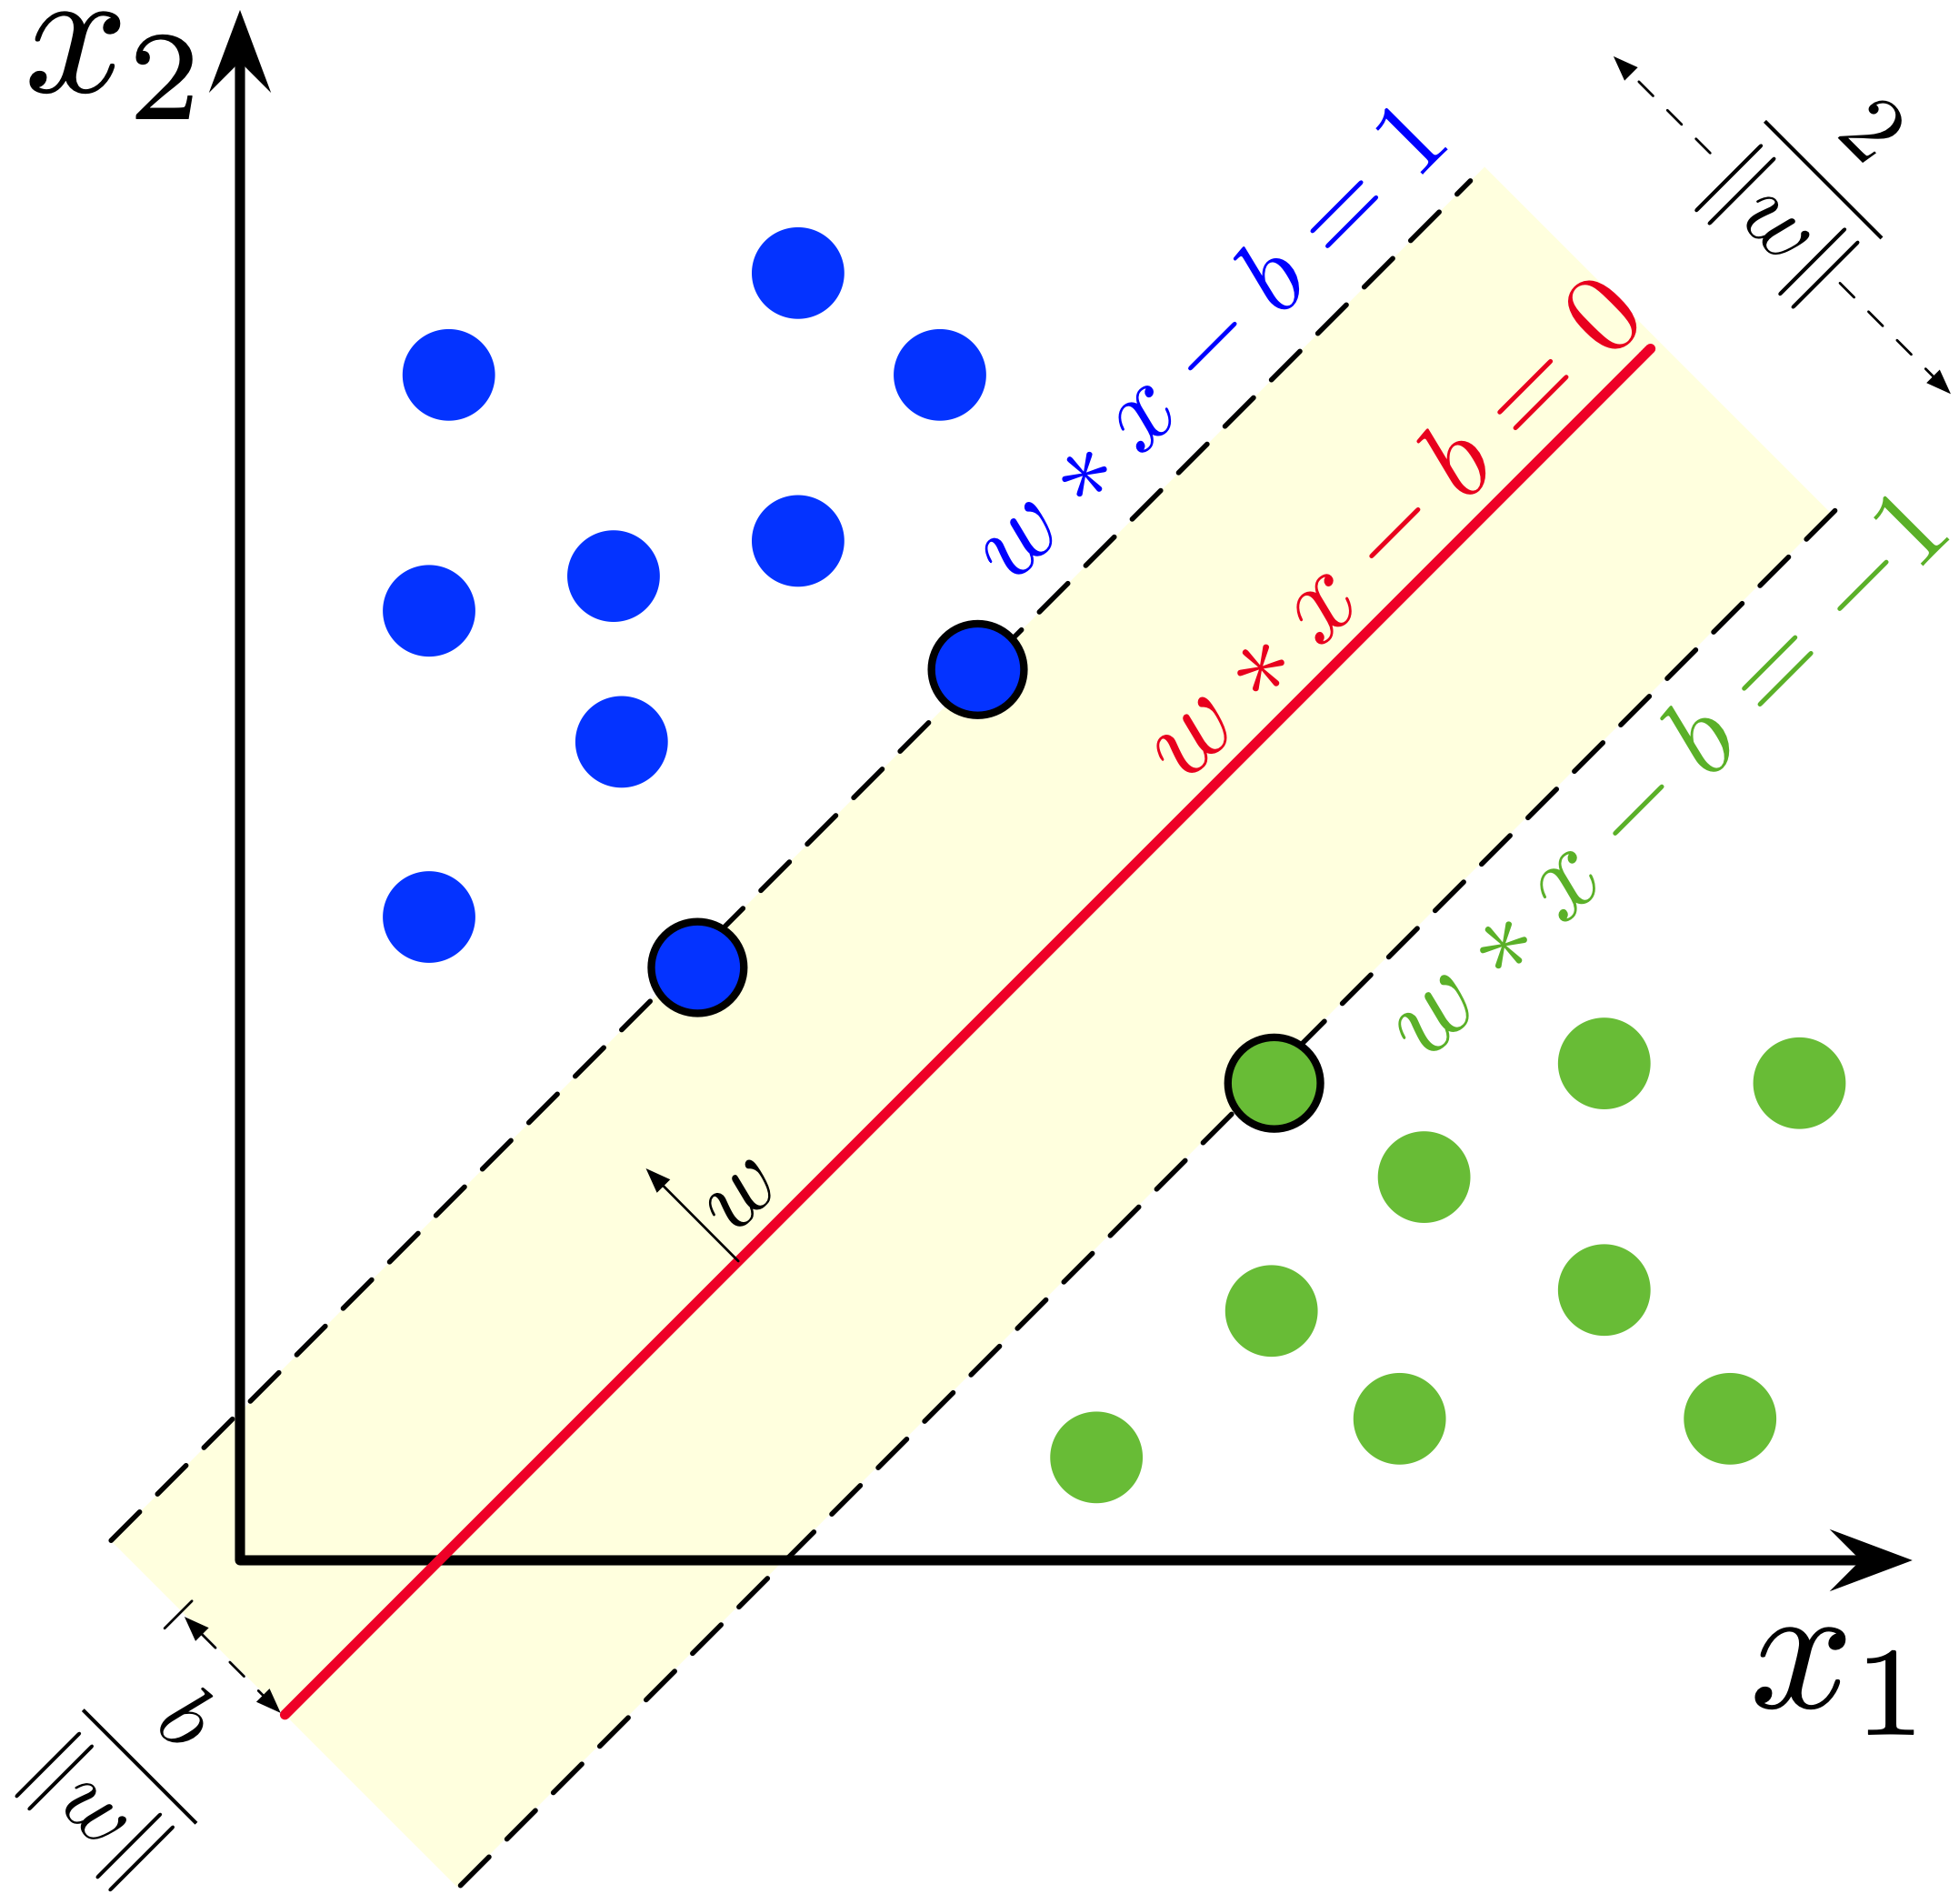
\includegraphics[width=0.7\textwidth]{svm_margin.png}
    \captionof{figure}{SVM tìm siêu phẳng (đường nét đứt) có lề (margin) rộng nhất giữa các lớp. Các điểm nằm trên lề được gọi là các vector hỗ trợ (support vectors).}
    \label{fig:svm_margin}
\end{center}

Việc tối đa hóa lề này giúp mô hình có khả năng tổng quát hóa tốt hơn trên dữ liệu mới, vì ranh giới quyết định ít bị ảnh hưởng bởi nhiễu.

\paragraph{The Kernel Trick}
Điểm mạnh thực sự của SVM nằm ở "thủ thuật kernel" (kernel trick). Nếu dữ liệu không thể phân tách bằng một đường thẳng, SVM có thể sử dụng một hàm kernel (ví dụ: RBF kernel) để ánh xạ dữ liệu lên một không gian nhiều chiều hơn, nơi chúng có thể trở nên phân tách tuyến tính. Điều này cho phép SVM học được các ranh giới quyết định phi tuyến rất phức tạp mà không cần tính toán trực tiếp trong không gian nhiều chiều đó, rất hiệu quả.

\paragraph{Huấn luyện và Hinge Loss}
Quá trình huấn luyện SVM là một bài toán tối ưu hóa nhằm tìm ra siêu phẳng có lề lớn nhất. Điều này được thực hiện bằng cách tối thiểu hóa một hàm mất mát đặc biệt gọi là \textbf{Hinge Loss}:
$$ \mathcal{L}(w) = \max(0, 1 - y_i(w^T x_i - b)) $$
Hàm mất mát này sẽ bằng 0 nếu một điểm dữ liệu nằm đúng phía của lề, và sẽ tăng tuyến tính nếu nó vi phạm lề. Việc tối ưu hóa này thường được giải quyết bằng các phương pháp phức tạp hơn như Quy hoạch toàn phương (Quadratic Programming).

\begin{tcolorbox}[
    title=Đánh giá SVM,
    colback=blue!5!white, colframe=blue!50!black, fonttitle=\bfseries
]
\textbf{Ưu điểm:}
\begin{itemize}
    \item \textbf{Hiệu quả cao trong không gian nhiều chiều:} Rất phù hợp với các vector TF-IDF có số chiều lớn.
    \item \textbf{Học được các ranh giới phi tuyến phức tạp:} Nhờ vào kernel trick.
    \item \textbf{Ít bị quá khớp (overfitting):} Do nguyên lý tối đa hóa lề.
\end{itemize}
\textbf{Nhược điểm:}
\begin{itemize}
    \item \textbf{Chi phí tính toán cao:} Huấn luyện SVM có thể rất chậm trên các bộ dữ liệu lớn.
    \item \textbf{Mô hình hộp đen (Black box):} Việc diễn giải một mô hình SVM với kernel phi tuyến là rất khó.
    \item \textbf{Nhạy cảm với việc lựa chọn kernel và tham số.}
\end{itemize}
\end{tcolorbox}


\subsection{Các mô hình Học chuỗi (Sequence Labeling Models)}
\label{ssec:sequence_models}
Các bài toán như Gán nhãn Từ loại (POS Tagging) hay Nhận dạng Thực thể Tên (NER) không chỉ đơn thuần là phân loại từng từ một cách độc lập. Nhãn của một từ phụ thuộc rất nhiều vào nhãn của các từ xung quanh. Các mô hình học chuỗi được thiết kế để giải quyết vấn đề này.

\subsubsection{Mô hình Markov ẩn (Hidden Markov Models - HMMs)}
HMM \cite{rabiner1989tutorial} là một mô hình sinh kinh điển cho các bài toán gán nhãn chuỗi.

\paragraph{Trực giác cốt lõi}
HMM giả định rằng một chuỗi các quan sát (observations) - tức là các từ trong câu - được "sinh ra" bởi một chuỗi các trạng thái ẩn (hidden states) - tức là các nhãn (ví dụ, các nhãn POS).
Quá trình sinh này tuân theo hai loại xác suất:
\begin{enumerate}
    \item \textbf{Xác suất chuyển trạng thái (Transition Probabilities):} Xác suất chuyển từ một trạng thái ẩn này sang một trạng thái ẩn khác. Ví dụ, $P(\text{Verb}|\text{Noun})$ - xác suất một động từ xuất hiện sau một danh từ. Điều này tuân theo giả định Markov.
    \item \textbf{Xác suất phát sinh (Emission Probabilities):} Xác suất một trạng thái ẩn "sinh ra" một từ quan sát được. Ví dụ, $P(\text{``sách''}|\text{Noun})$ - xác suất từ "sách" được sinh ra khi trạng thái ẩn là Danh từ.
\end{enumerate}

\begin{center}
    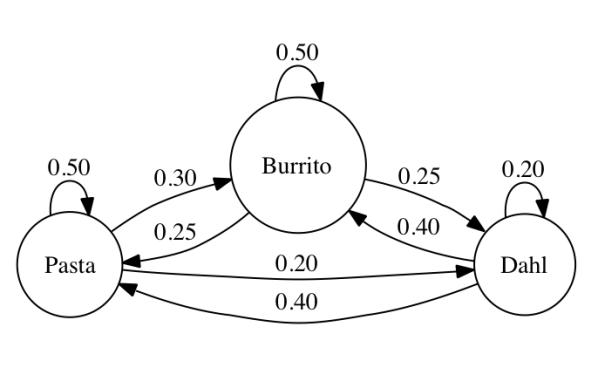
\includegraphics[width=0.8\textwidth]{hmm_diagram.png}
    \captionof{figure}{Sơ đồ một chuỗi Markov (Markov chain) với ba trạng thái: Pasta, Burrito, và Dahl. Các con số biểu thị xác suất chuyển đổi giữa các trạng thái.}
    \label{fig:hmm_diagram}
\end{center}

Nhiệm vụ của HMM là tìm ra chuỗi trạng thái ẩn (chuỗi nhãn) có khả năng nhất đã sinh ra chuỗi các từ quan sát được. Bài toán này được giải quyết hiệu quả bằng một thuật toán quy hoạch động gọi là \textbf{Thuật toán Viterbi (Viterbi Algorithm)}.

\subsubsection{Trường Ngẫu nhiên Có điều kiện (Conditional Random Fields - CRFs)}
CRF, và đặc biệt là Linear-chain CRF, là một cải tiến vượt bậc so với HMM và đã trở thành mô hình thống kê tiêu chuẩn cho các bài toán gán nhãn chuỗi trong nhiều năm.

\paragraph{Sự khác biệt chính với HMM}
HMM là một mô hình sinh, nó mô hình hóa xác suất kết hợp $P(\text{chuỗi quan sát, chuỗi nhãn})$. CRF là một mô hình phân biệt, nó mô hình hóa trực tiếp xác suất có điều kiện $P(\text{chuỗi nhãn}|\text{chuỗi quan sát})$.
Sự thay đổi này mang lại hai lợi thế lớn:
\begin{enumerate}
    \item \textbf{Bỏ giả định độc lập của đặc trưng:} HMM giả định rằng một từ quan sát chỉ phụ thuộc vào trạng thái ẩn hiện tại. CRF không có giả định này. Nó có thể sử dụng một loạt các đặc trưng phức tạp của chuỗi đầu vào, ví dụ: "từ hiện tại có viết hoa không?", "hậu tố của từ hiện tại là gì?", "từ trước đó là gì?". Điều này làm cho CRF linh hoạt và mạnh mẽ hơn nhiều.
    \item \textbf{Tránh tính toán $P(\text{chuỗi quan sát})$:} Việc mô hình hóa xác suất của chuỗi quan sát là rất khó, CRF đã loại bỏ được gánh nặng này.
\end{enumerate}

\paragraph{Trực giác cốt lõi của CRF}
Thay vì tính toán các xác suất chuyển và phát sinh riêng lẻ, một CRF gán một điểm số (score) cho mỗi cặp (chuỗi quan sát, chuỗi nhãn) dựa trên một tổ hợp tuyến tính của các hàm đặc trưng (feature functions). Các hàm đặc trưng này có thể bắt các mối quan hệ phức tạp giữa các từ và nhãn. Sau đó, nó sử dụng một hàm chuẩn hóa (tương tự softmax) trên toàn bộ các chuỗi nhãn có thể có để biến điểm số thành xác suất. Nhiệm vụ cũng là tìm ra chuỗi nhãn có xác suất (điểm số) cao nhất, và cũng thường được giải bằng thuật toán Viterbi.

\begin{tcolorbox}[
    title=So sánh HMM và CRF,
    colback=green!5!white, colframe=green!60!black, fonttitle=\bfseries
]
\begin{tabular}{p{0.45\linewidth} | p{0.45\linewidth}}
    \textbf{Hidden Markov Models (HMM)} & \textbf{Conditional Random Fields (CRF)} \\
    \hline
    Mô hình \textbf{sinh} (Generative) & Mô hình \textbf{phân biệt} (Discriminative) \\
    \hline
    Mô hình hóa $P(\text{observations, labels})$ & Mô hình hóa $P(\text{labels | observations})$ \\
    \hline
    Giả định các quan sát độc lập có điều kiện & Không có giả định độc lập, cho phép các đặc trưng chồng chéo, phức tạp. \\
    \hline
    Huấn luyện nhanh hơn & Huấn luyện chậm hơn (cần các thuật toán lặp) \\
    \hline
    Thường cho hiệu năng thấp hơn & Thường cho hiệu năng \textbf{vượt trội}, là state-of-the-art trong kỷ nguyên thống kê. \\
\end{tabular}
\end{tcolorbox}
% % !TEX root = ../../main.tex
% File: part2/chapters2/chap2_4.tex

\section{Huấn luyện Phân tán (Distributed Training)}
\label{sec:distributed_training}

Khi quy mô của các mô hình ngôn ngữ tăng từ hàng trăm triệu lên hàng tỷ, thậm chí hàng nghìn tỷ tham số, việc huấn luyện chúng trên một GPU duy nhất trở nên bất khả thi. Ngay cả những GPU mạnh nhất cũng không đủ bộ nhớ (VRAM) để chứa toàn bộ trọng số, gradient, và trạng thái của optimizer.

\textbf{Huấn luyện Phân tán} là một tập hợp các kỹ thuật cho phép chúng ta chia nhỏ gánh nặng tính toán và bộ nhớ của quá trình huấn luyện ra \textbf{nhiều GPU} (trên một hoặc nhiều máy).

\subsection{Các Mô hình Song song (Parallelism Paradigms)}
\label{ssec:parallelism_paradigms}
Có nhiều cách khác nhau để "chia nhỏ" quá trình huấn luyện. Ba chiến lược chính là:

\begin{enumerate}
    \item \textbf{Data Parallelism (DP) - Song song Dữ liệu:}
        \begin{itemize}
            \item \textbf{Ý tưởng:} Đây là chiến lược phổ biến và đơn giản nhất. Mỗi GPU sẽ giữ một \textbf{bản sao đầy đủ của mô hình}. Dữ liệu huấn luyện (batch) sẽ được chia nhỏ ra, và mỗi GPU sẽ xử lý một phần của batch đó.
            \item \textbf{Quy trình:} Các GPU tính toán gradient một cách độc lập trên phần dữ liệu của mình, sau đó chúng "giao tiếp" với nhau để đồng bộ hóa và tính trung bình các gradient trước khi cập nhật trọng số.
            \item \textbf{Hạn chế:} Không giải quyết được vấn đề bộ nhớ. Nếu mô hình quá lớn để vừa trên một GPU, DP sẽ không hoạt động.
        \end{itemize}
    \item \textbf{Tensor Parallelism (TP) - Song song Tensor:}
        \begin{itemize}
            \item \textbf{Ý tưởng:} Thay vì sao chép mô hình, chúng ta chia nhỏ \textbf{chính các ma trận trọng số} của mô hình ra nhiều GPU.
            \item \textbf{Quy trình:} Ví dụ, một phép nhân ma trận lớn có thể được chia thành nhiều phép nhân ma trận nhỏ hơn được thực hiện song song trên các GPU khác nhau. Các GPU cần giao tiếp với nhau rất nhiều trong quá trình truyền thẳng và truyền ngược.
            \item \textbf{Lợi ích:} Cho phép huấn luyện các mô hình lớn hơn bộ nhớ của một GPU.
        \end{itemize}
    \item \textbf{Pipeline Parallelism (PP) - Song song Đường ống:}
        \begin{itemize}
            \item \textbf{Ý tưởng:} Chia các \textbf{lớp (layers)} của mô hình ra nhiều GPU.
            \item \textbf{Quy trình:} GPU 1 sẽ xử lý các lớp đầu tiên (ví dụ: 0-11), sau đó chuyển kết quả đầu ra cho GPU 2 để xử lý các lớp tiếp theo (ví dụ: 12-23), và cứ thế tiếp tục. Nó hoạt động giống như một dây chuyền lắp ráp.
            \item \textbf{Hạn chế:} Có thể gây ra "bong bóng" (bubbles), tức là thời gian chờ khi các GPU ở đầu đường ống phải đợi các GPU ở cuối hoàn thành công việc.
        \end{itemize}
\end{enumerate}

Trong thực tế, các hệ thống huấn luyện LLM quy mô lớn thường kết hợp cả ba loại song song này (cùng với các kỹ thuật khác) để đạt được hiệu quả cao nhất.

\subsection{Sử dụng `accelerate` và `DeepSpeed` để Huấn luyện Mô hình lớn}
\label{ssec:accelerate_deepspeed}
Việc triển khai các chiến lược song song này từ đầu là cực kỳ phức tạp. May mắn thay, chúng ta có các thư viện mạnh mẽ giúp tự động hóa quá trình này.

\subsubsection{Accelerate: Giao diện Tối giản}
Như đã giới thiệu ở mục \ref{ssec:hf_accelerate}, `accelerate` cung cấp một giao diện đơn giản để chạy code PyTorch trên nhiều môi trường phần cứng.
\begin{itemize}
    \item \textbf{Cách hoạt động:}
        \begin{enumerate}
            \item Bạn viết một kịch bản huấn luyện PyTorch tiêu chuẩn.
            \item Chạy lệnh `accelerate config` trong terminal để thiết lập môi trường của bạn (ví dụ: "sử dụng 2 GPU trên máy này", "sử dụng precision fp16").
            \item Chạy kịch bản của bạn bằng lệnh `accelerate launch your\_script.py`.
        \end{enumerate}
    \item \textbf{Tích hợp với `Trainer`:} `Trainer` của Hugging Face đã tích hợp sẵn `accelerate`. Khi bạn chạy một kịch bản `Trainer` với `accelerate launch`, nó sẽ tự động áp dụng chiến lược Data Parallelism (DP) trên các GPU có sẵn.
\end{itemize}
`accelerate` là lựa chọn tuyệt vời để dễ dàng song song hóa dữ liệu. Nhưng khi mô hình trở nên quá lớn, chúng ta cần một công cụ mạnh mẽ hơn.

\subsubsection{DeepSpeed: Cỗ máy Tối ưu hóa Toàn diện}
DeepSpeed là một thư viện mã nguồn mở từ Microsoft, cung cấp một bộ công cụ tối ưu hóa cực kỳ mạnh mẽ để huấn luyện các mô hình khổng lồ. Nó không chỉ là một chiến lược song song, mà là một hệ thống toàn diện.

\begin{tcolorbox}[
    title=ZeRO: Tối ưu hóa Bộ nhớ Cách mạng,
    colback=green!5!white, colframe=green!60!black, fonttitle=\bfseries
]
Phát kiến cốt lõi của DeepSpeed là \textbf{ZeRO (Zero Redundancy Optimizer)}. ZeRO nhận ra rằng trong Data Parallelism thông thường, mỗi GPU đều lưu trữ một cách thừa thãi các bản sao của \textbf{trọng số mô hình}, \textbf{gradient}, và \textbf{trạng thái optimizer}. ZeRO loại bỏ sự thừa thãi này bằng cách \textbf{phân mảnh (partitioning)} các thành phần này ra tất cả các GPU.
\end{tcolorbox}

\paragraph{Các Giai đoạn của ZeRO}
\begin{itemize}
    \item \textbf{ZeRO-1:} Phân mảnh \textbf{trạng thái optimizer}. Mỗi GPU chỉ giữ một phần của trạng thái optimizer. Giảm bộ nhớ đáng kể.
    \item \textbf{ZeRO-2:} Phân mảnh cả \textbf{trạng thái optimizer} và \textbf{gradient}. Mỗi GPU chỉ tính và lưu trữ một phần của gradient. Giảm bộ nhớ nhiều hơn nữa.
    \item \textbf{ZeRO-3:} Phân mảnh tất cả: \textbf{trạng thái optimizer}, \textbf{gradient}, và cả \textbf{trọng số mô hình}. Mỗi GPU chỉ giữ một lát cắt (slice) của mô hình. Trong quá trình truyền thẳng/ngược, các GPU sẽ giao tiếp với nhau để tập hợp lại các lớp cần thiết ngay khi cần. Đây là giai đoạn mạnh mẽ nhất, cho phép huấn luyện các mô hình nghìn tỷ tham số.
\end{itemize}

\begin{center}
    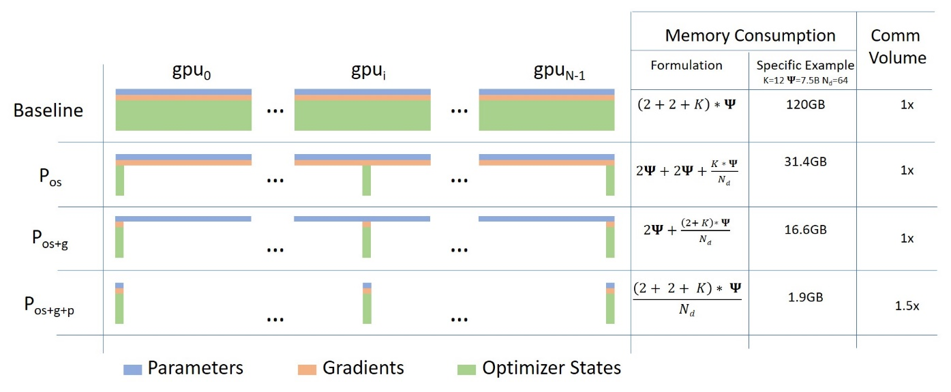
\includegraphics[width=1.0\textwidth]{deepspeed_zero.png}
    \captionof{figure}{So sánh việc sử dụng bộ nhớ trong Data Parallelism tiêu chuẩn và các giai đoạn của ZeRO. ZeRO giảm đáng kể sự thừa thãi bằng cách phân mảnh các thành phần của quá trình huấn luyện.}
    \label{fig:deepspeed_zero}
\end{center}

\paragraph{Tích hợp DeepSpeed với `Trainer`}
Sức mạnh của hệ sinh thái Hugging Face là việc tích hợp các công cụ phức tạp này trở nên rất đơn giản.
\begin{enumerate}
    \item \textbf{Tạo file cấu hình DeepSpeed:} Tạo một file JSON (ví dụ: `ds\_config.json`) để định nghĩa các thiết lập bạn muốn sử dụng (ví dụ: bật ZeRO-2, sử dụng precision fp16, thiết lập optimizer).
    \item \textbf{Truyền vào `TrainingArguments`:}
        \begin{tcolorbox}[title=Cấu hình DeepSpeed, colback=black!5!white, colframe=black!80!white]
            \begin{minted}[linenos, numbersep=0pt]{python}
            training_args = TrainingArguments(
                output_dir="./results",
                # ...
                deepspeed="path/to/your/ds_config.json", # Chỉ định file config
            )
            \end{minted}
        \end{tcolorbox}
    \item \textbf{Khởi chạy:} Sử dụng `deepspeed your\_script.py` hoặc `accelerate launch --use\_deepspeed your\_script.py` để chạy kịch bản.
\end{enumerate}
`Trainer` và `accelerate` sẽ tự động xử lý tất cả các chi tiết phức tạp của việc khởi tạo và chạy DeepSpeed.

Ngoài ZeRO, DeepSpeed còn cung cấp nhiều tính năng tối ưu hóa khác như \textbf{Offloading} (chuyển bớt các tham số không dùng đến từ VRAM sang CPU RAM hoặc NVMe) và các kernel hiệu năng cao. Bằng cách kết hợp các công cụ như `accelerate` và `DeepSpeed`, việc huấn luyện các mô hình ngôn ngữ lớn không còn là đặc quyền của một vài phòng thí nghiệm AI lớn, mà đã trở nên dễ tiếp cận hơn với cộng đồng nghiên cứu và các doanh nghiệp.

\bigskip
\hrule
\bigskip

\begin{center}
    \textbf{\Large KẾT THÚC CHƯƠNG 2}
\end{center}

\textit{Chương 2 đã trang bị cho bạn một bộ công cụ thực chiến hoàn chỉnh, từ việc làm quen với hệ sinh thái Hugging Face, xây dựng các quy trình đánh giá đáng tin cậy, đến việc quản lý các thí nghiệm một cách khoa học và huấn luyện các mô hình trên quy mô lớn. Với những kỹ năng này, bạn đã sẵn sàng để đối mặt với những thách thức phức tạp hơn trong việc triển khai và vận hành các hệ thống NLP trong môi trường production, chủ đề của chương tiếp theo.}

% \chapter{CÁC KIẾN TRÚC MẠNG NƠ-RON KINH ĐIỂN}
\label{chap:deep_learning_architectures}

Chào mừng bạn đến với kỷ nguyên học sâu của NLP. Trong chương 2, chúng ta đã thấy các mô hình thống kê như N-gram có thể nắm bắt các phụ thuộc cục bộ, nhưng lại bất lực trước các mối quan hệ tầm xa. Cuộc cách mạng word embedding đã cho chúng ta các vector từ mang đầy ngữ nghĩa, nhưng làm thế nào để kết hợp chúng lại nhằm hiểu được ý nghĩa của cả một câu hay một đoạn văn?

Chương này sẽ giới thiệu các kiến trúc mạng nơ-ron nền tảng được thiết kế đặc biệt để xử lý dữ liệu dạng chuỗi như ngôn ngữ tự nhiên. Những kiến trúc này không chỉ đơn thuần "nhìn" vào các từ một cách riêng lẻ, mà còn có khả năng "ghi nhớ" và "lý luận" dựa trên thông tin đã xử lý trước đó, cho phép chúng nắm bắt được ngữ cảnh và các phụ thuộc phức tạp trong câu.
% % !TEX root = ../main.tex
% File: chapters_part1/chap3_1.tex
% Nội dung cho Phần 3.1: Word Embeddings

\section{Word Embeddings: Cuộc cách mạng Biểu diễn Đầu tiên}
\label{sec:word_embeddings}

Các phương pháp biểu diễn dựa trên tần suất như BoW hay TF-IDF, mặc dù hữu ích, lại mắc phải hai nhược điểm chí mạng:
\begin{enumerate}
    \item \textbf{Độ thưa thớt (Sparsity):} Chúng tạo ra các vector có số chiều khổng lồ và hầu hết là số 0.
    \item \textbf{Thiếu vắng ngữ nghĩa (Lack of Semantics):} Các vector này không hề nắm bắt được mối quan hệ ngữ nghĩa giữa các từ. Đối với BoW, hai từ "tốt" và "tuyệt vời" là hoàn toàn khác biệt, không có mối liên hệ nào.
\end{enumerate}

\textbf{Word Embeddings} (Nhúng từ) ra đời để giải quyết triệt để hai vấn đề trên. Đây là một tập hợp các kỹ thuật học máy có mục tiêu biểu diễn mỗi từ trong từ vựng bằng một \textbf{vector dày đặc (dense vector)} có số chiều tương đối thấp (thường từ 50 đến 300 chiều). Quan trọng hơn, các vector này được học sao cho chúng có thể nắm bắt được các mối quan hệ ngữ nghĩa và cú pháp giữa các từ.

Ý tưởng nền tảng của Word Embeddings dựa trên \textbf{Giả thuyết Phân bố (Distributional Hypothesis)} của Firth (1957), được tóm gọn trong câu nói nổi tiếng:
\begin{tcolorbox}[
    title=Giả thuyết Phân bố,
    colback=yellow!10!white, colframe=yellow!50!black, fonttitle=\bfseries
]
"You shall know a word by the company it keeps." (Bạn có thể hiểu một từ qua những từ thường đi cùng với nó.)
\end{tcolorbox}
Nói cách khác, những từ xuất hiện trong các ngữ cảnh tương tự nhau thì có khả năng mang ý nghĩa tương tự nhau. Word Embeddings là hiện thực hóa của giả thuyết này bằng các mô hình mạng nơ-ron.

\subsection{Lý thuyết Word2Vec: CBOW \& Skip-gram}
\label{ssec:word2vec}
Được giới thiệu bởi Tomas Mikolov và các cộng sự tại Google vào năm 2013 \cite{mikolov2013efficient, mikolov2013distributed}, Word2Vec không phải là một thuật toán duy nhất mà là một bộ công cụ bao gồm hai kiến trúc mô hình chính: \textbf{CBOW (Continuous Bag-of-Words)} và \textbf{Skip-gram}. Word2Vec đã tạo ra một cuộc cách mạng trong lĩnh vực Xử lý Ngôn ngữ Tự nhiên (NLP), dân chủ hóa việc sử dụng \textit{word embeddings} nhờ vào hiệu quả tính toán và chất lượng của vector biểu diễn mà nó tạo ra.

\subsubsection{Kiến trúc chung: Mạng Nơ-ron Nông}
\label{sssec:w2v_architecture}
Cốt lõi của Word2Vec là một ý tưởng đơn giản đến bất ngờ: thay vì xây dựng một mô hình ngôn ngữ phức tạp, chúng ta thiết kế một nhiệm vụ "giả" (fake task) và trong quá trình huấn luyện mô hình để giải quyết nhiệm vụ đó, chúng ta sẽ học được các vector từ chất lượng cao.

\paragraph{Nhiệm vụ "giả" so với Mô hình Ngôn ngữ "thật"}
Gọi là "giả" vì mục tiêu cuối cùng của chúng ta không phải là giải quyết tốt nhiệm vụ dự đoán từ, mà là học được ma trận trọng số \textbf{W}. Một mô hình ngôn ngữ "thật" (true language model), chẳng hạn như các mô hình dựa trên RNN, sẽ có mục tiêu phức tạp hơn nhiều: dự đoán từ tiếp theo dựa trên toàn bộ lịch sử các từ trước đó ($P(w_t | w_1, ..., w_{t-1})$). Việc này đòi hỏi kiến trúc sâu và phức tạp hơn.

Ngược lại, Word2Vec đơn giản hóa triệt để vấn đề: nó chỉ dự đoán từ dựa trên một cửa sổ ngữ cảnh cục bộ nhỏ. Sự đơn giản hóa này chính là chìa khóa thành công: nó cho phép mô hình xử lý hiệu quả một lượng dữ liệu văn bản khổng lồ. Gradient từ nhiệm vụ đơn giản này, tuy không hoàn hảo cho việc dự đoán ngôn ngữ, lại cực kỳ hiệu quả trong việc định hình một không gian vector mà ở đó các từ có ngữ cảnh tương tự được đặt gần nhau.

Cả CBOW và Skip-gram đều sử dụng kiến trúc mạng nơ-ron "nông" (shallow) chỉ với một lớp ẩn duy nhất. Giả sử từ vựng của chúng ta có \textbf{V} từ độc nhất và chúng ta muốn học các vector biểu diễn có \textbf{N} chiều (embedding dimension).

\begin{itemize}
    \item \textbf{Lớp vào (Input Layer):} Đầu vào là một vector \textit{one-hot} có kích thước $1 \times V$, đại diện cho một từ.
    \item \textbf{Lớp ẩn (Hidden Layer):} Không có hàm kích hoạt. Điểm mấu chốt nằm ở ma trận trọng số \textbf{W} kết nối lớp vào và lớp ẩn. Ma trận này có kích thước $V \times N$.
    \item \textbf{Lớp ra (Output Layer):} Ma trận trọng số \textbf{W'} kết nối lớp ẩn và lớp ra, có kích thước $N \times V$.
\end{itemize}

\begin{tcolorbox}[
    title=Ghi chú về Thiết kế Kiến trúc,
    colback=green!5!white, colframe=green!50!black, fonttitle=\bfseries
]
\textbf{1. Tại sao không có hàm kích hoạt ở lớp ẩn?} \\
Lớp ẩn của Word2Vec thực chất là một lớp tuyến tính (linear projection). Việc loại bỏ hàm phi tuyến (như ReLU hay Tanh) là một lựa chọn có chủ ý. Mục đích là để các mối quan hệ ngữ nghĩa (ví dụ: các phép loại suy -- analogies) có thể được biểu diễn dưới dạng các phép toán vector tuyến tính đơn giản (ví dụ: $\vec{v}_{\text{king}} - \vec{v}_{\text{man}} + \vec{v}_{\text{woman}} \approx \vec{v}_{\text{queen}}$). Nếu thêm hàm phi tuyến, cấu trúc tuyến tính này sẽ bị phá vỡ, làm cho các vector học được khó diễn giải và sử dụng hơn theo cách này. Lớp ẩn chỉ đóng vai trò như một bảng tra cứu (lookup table) để lấy ra vector embedding.

\textbf{2. Tại sao có hai ma trận trọng số W và W'?} \\
Mô hình có hai bộ vector cho mỗi từ:
\begin{itemize}
    \item \textbf{Input vectors (trong W):} Khi từ được dùng làm đầu vào (từ trung tâm trong Skip-gram, từ ngữ cảnh trong CBOW).
    \item \textbf{Output vectors (trong W'):} Khi từ được dùng làm mục tiêu dự đoán (từ ngữ cảnh trong Skip-gram, từ trung tâm trong CBOW).
\end{itemize}
Về mặt lý thuyết, việc có hai vai trò riêng biệt cho phép mô hình linh hoạt hơn. Sau khi huấn luyện xong, chúng ta thường chỉ sử dụng ma trận đầu vào \textbf{W} làm embedding cuối cùng. Đây là một quy ước phổ biến và cho kết quả tốt trong thực tế. Một số nghiên cứu cũng đề xuất các cách kết hợp khác (ví dụ, lấy trung bình cộng của hai vector tương ứng từ \textbf{W} và \textbf{W'}), nhưng chỉ dùng \textbf{W} vẫn là phương pháp tiêu chuẩn.
\end{tcolorbox}

Điều quan trọng là, chúng ta không thực sự quan tâm đến kết quả dự đoán của mạng. Mục tiêu cuối cùng của chúng ta là học được ma trận trọng số \textbf{W}. Sau khi huấn luyện, mỗi hàng của ma trận \textbf{W} chính là vector embedding N-chiều cho một từ tương ứng trong từ vựng. Do đó, \textbf{W} còn được gọi là \textbf{ma trận embedding (embedding matrix)}.

\begin{center}
    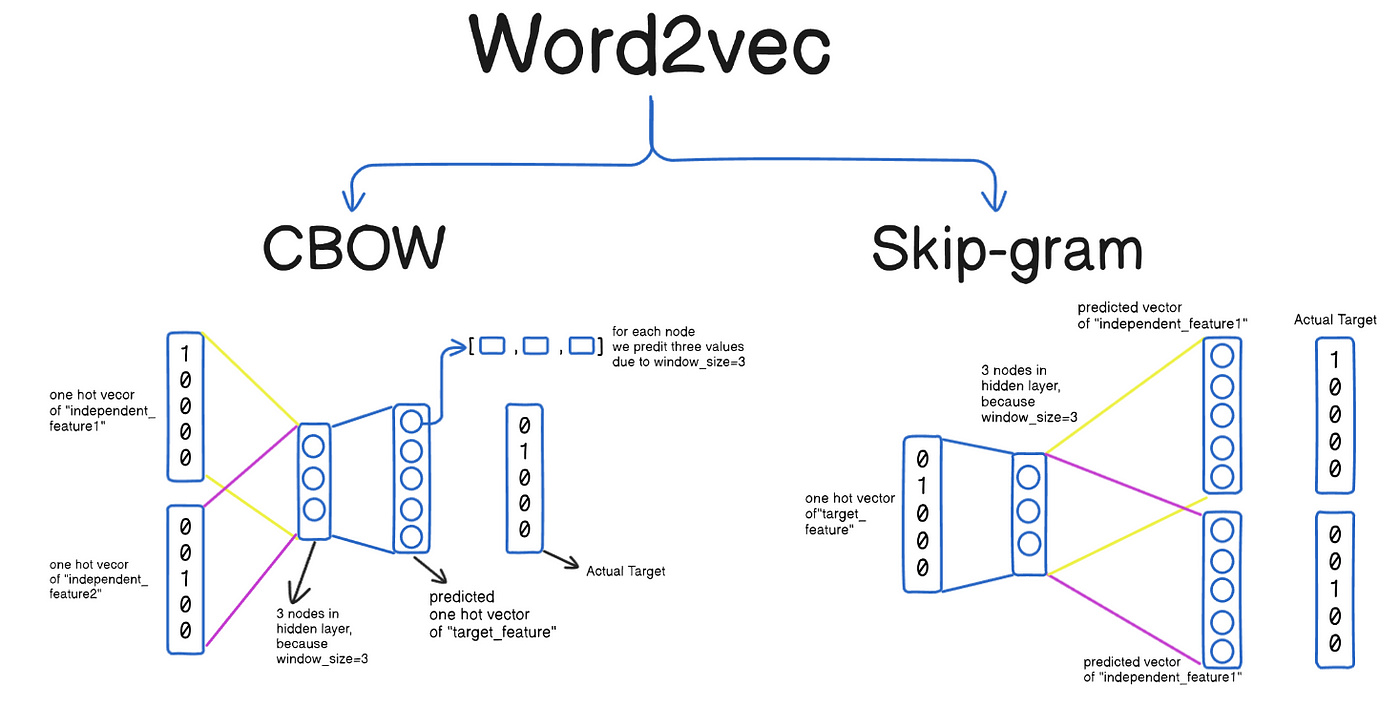
\includegraphics[width=0.8\textwidth]{word2vec_architecture.png}
    \captionof{figure}{Kiến trúc chung của Word2Vec. Khi nhân vector one-hot của một từ với ma trận $W$, thực chất chúng ta đang "chọn" ra hàng tương ứng với từ đó, chính là vector embedding của nó. Ma trận $W$ là mục tiêu chúng ta cần học.}
    \label{fig:word2vec_architecture}
\end{center}

\subsubsection{Mô hình CBOW (Continuous Bag-of-Words)}
\paragraph{Tư duy cốt lõi}
Mô hình CBOW hoạt động dựa trên giả định: "Một từ có thể được dự đoán bởi các từ xung quanh nó". Do đó, CBOW cố gắng \textbf{dự đoán một từ trung tâm (center word) dựa vào các từ ngữ cảnh (context words)}.

Ví dụ, trong câu "chú mèo [ngồi] trên chiếc chiếu" và cửa sổ ngữ cảnh là 2, CBOW sẽ lấy các từ ngữ cảnh \texttt{\{"chú", "mèo", "trên", "chiếc"\}} để dự đoán từ trung tâm là \texttt{\{"ngồi"\}}.

\paragraph{Cơ chế hoạt động}
\begin{enumerate}
    \item \textbf{Đầu vào:} Lấy các vector one-hot của các từ ngữ cảnh (ví dụ: \texttt{chú}, \texttt{mèo}, \texttt{trên}, \texttt{chiếc}).
    \item \textbf{Lấy vector embedding:} Từ ma trận embedding \textbf{W}, ta lấy ra các vector embedding tương ứng cho từng từ ngữ cảnh.
    \item \textbf{Tổng hợp ngữ cảnh:} Các vector embedding này được \textbf{lấy trung bình cộng} để tạo thành một vector ngữ cảnh duy nhất $\mathbf{v}_{\text{context}}$. Việc lấy trung bình này giải thích cho tên gọi "Bag-of-Words", vì nó làm mất đi thông tin về thứ tự các từ trong ngữ cảnh.
    \item \textbf{Dự đoán:} Vector $\mathbf{v}_{\text{context}}$ được nhân với ma trận \textbf{W'} và đưa qua hàm \textbf{softmax} để tạo ra một phân phối xác suất trên toàn bộ từ vựng. Vector đầu ra $\hat{\mathbf{y}}$ có kích thước $1 \times V$, trong đó phần tử thứ $j$ biểu diễn xác suất từ trung tâm là từ thứ $j$ trong từ vựng.
    \item \textbf{Huấn luyện:} So sánh vector xác suất dự đoán $\hat{\mathbf{y}}$ với vector one-hot $\mathbf{y}$ của từ trung tâm thực tế (từ \texttt{ngồi}). Hàm mất mát thường được sử dụng là \textbf{Cross-Entropy}, và lỗi được lan truyền ngược (backpropagation) để cập nhật các trọng số trong cả hai ma trận \textbf{W} và \textbf{W'}.
    $$ \mathcal{L} = -\sum_{j=1}^{V} y_j \log(\hat{y}_j) $$
\end{enumerate}

\paragraph{Phân tích lựa chọn thiết kế của CBOW}
Việc lấy trung bình các vector ngữ cảnh là một lựa chọn thiết kế vì sự đơn giản và hiệu quả tính toán. Nó không cần tham số nào để học và có thể được tính rất nhanh. Tuy nhiên, lựa chọn này có hai hệ quả quan trọng:
\begin{itemize}
    \item \textbf{Mất thông tin thứ tự:} CBOW không phân biệt được hai câu có cùng các từ ngữ cảnh nhưng khác trật tự. Trong nhiều tác vụ, việc mất thông tin cú pháp này là một hạn chế đáng kể.
    \item \textbf{"Lu mờ" từ hiếm:} Khi lấy trung bình, đóng góp của một vector từ hiếm có thể bị "lấn át" bởi các vector của các từ ngữ cảnh phổ biến hơn. Đây là lý do CBOW thường hoạt động kém hơn Skip-gram đối với các từ hiếm.
\end{itemize}
Các phương pháp phức tạp hơn như lấy trung bình có trọng số (dựa trên khoảng cách tới từ trung tâm) hoặc thậm chí dùng một cơ chế attention đơn giản có thể được xem xét, nhưng chúng sẽ làm tăng độ phức tạp và đi ngược lại triết lý "đơn giản, nhanh" của Word2Vec.

\subsubsection{Mô hình Skip-gram}
\paragraph{Tư duy cốt lõi}
Skip-gram đảo ngược lại nhiệm vụ của CBOW. Nó hoạt động dựa trên giả định: "Một từ có thể cho biết những từ nào sẽ xuất hiện xung quanh nó". Do đó, Skip-gram cố gắng \textbf{dự đoán các từ ngữ cảnh dựa vào một từ trung tâm}.

Ví dụ, với cùng câu trên, Skip-gram sẽ lấy từ trung tâm \texttt{\{"ngồi"\}} để cố gắng dự đoán từng từ trong tập ngữ cảnh \texttt{\{"chú", "mèo", "trên", "chiếc"\}}.

\paragraph{Cơ chế hoạt động}
Khác với CBOW, Skip-gram không gộp ngữ cảnh lại. Thay vào đó, nó tạo ra nhiều mẫu huấn luyện hơn từ một cửa sổ ngữ cảnh.
\begin{enumerate}
    \item \textbf{Đầu vào:} Lấy vector one-hot của từ trung tâm (ví dụ: \texttt{ngồi}).
    \item \textbf{Lấy vector embedding:} Lấy ra vector embedding $\mathbf{v}_{\text{center}}$ của từ trung tâm từ ma trận \textbf{W}.
    \item \textbf{Dự đoán:} Vector $\mathbf{v}_{\text{center}}$ được đưa thẳng đến lớp ra (nhân với \textbf{W'} và qua hàm softmax) để tạo ra một vector xác suất $\hat{\mathbf{y}}$.
    \item \textbf{Huấn luyện:} Quá trình này được lặp lại cho \textbf{từng từ trong ngữ cảnh}. Với mỗi cặp (\texttt{từ trung tâm}, \texttt{từ ngữ cảnh}), một hàm mất mát \textbf{Cross-Entropy} được tính toán giữa dự đoán $\hat{\mathbf{y}}$ và vector one-hot của từ ngữ cảnh thực tế. Tổng các lỗi từ tất cả các cặp được sử dụng để cập nhật trọng số qua backpropagation. Điều này giúp Skip-gram học được các biểu diễn tinh vi hơn, đặc biệt cho các từ hiếm, nhưng cũng tốn nhiều thời gian huấn luyện hơn.
\end{enumerate}

\begin{center}
    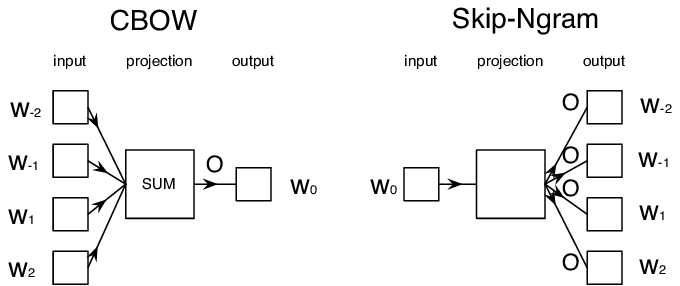
\includegraphics[width=0.9\textwidth]{cbow_skipgram_diagram.png}
    \captionof{figure}{So sánh trực quan giữa CBOW (tổng hợp ngữ cảnh để dự đoán 1 từ) và Skip-gram (dùng 1 từ để dự đoán nhiều từ trong ngữ cảnh, tạo thành các cặp huấn luyện riêng biệt).}
    \label{fig:cbow_skipgram_diagram}
\end{center}

\subsubsection{Vì sao Word2Vec học được ngữ nghĩa và gần--xa theo cosine?}
\label{sssec:w2v_why_semantics}

\paragraph{Nguyên lý phân bố (Distributional Hypothesis).}
Từ ngữ xuất hiện trong \emph{ngữ cảnh} giống nhau thường có nghĩa giống nhau. Khi huấn luyện Word2Vec để dự đoán từ--ngữ cảnh, các vector bị tối ưu sao cho những từ chia sẻ nhiều ngữ cảnh sẽ có \emph{hướng} gần nhau trong không gian.

\paragraph{CBOW: gom ngữ cảnh để dự đoán từ.}
Gọi $C$ là tập ngữ cảnh, $|C|=m$, $v_c \in \mathbb{R}^N$ là embedding của từ $c\in C$, và $u_w \in \mathbb{R}^N$ là vector ``ra'' cho từ trung tâm $w$. CBOW tính
\[
h \;=\; \frac{1}{m}\sum_{c\in C} v_c,\qquad 
p(w\,|\,C) \;=\; \mathrm{softmax}\big(u_w^\top h\big).
\]
Tối đa hoá $\log p(w\,|\,C)$ khiến $u_w^\top h$ tăng. Do $h$ là trung bình các $v_c$, mọi $v_c$ đều nhận gradient đẩy \emph{đồng hướng} với $u_w$. Khi hai từ $w_1,w_2$ thường cùng chia sẻ ngữ cảnh, các cập nhật lặp đi lặp lại làm $v_{w_1},v_{w_2}$ trở nên \emph{đồng hướng}.

\paragraph{Skip-gram với Negative Sampling (SGNS): kéo--đẩy cục bộ.}
Với cặp dương $(w,c)$ và các âm $n\in\mathcal{N}$, hàm mục tiêu một bước là
\[
\mathcal{L}_{\text{SGNS}} \;=\; 
- \log \sigma\!\big(u_c^\top v_w\big) \;-\; \sum_{n\in\mathcal{N}} \log \sigma\!\big(-u_n^\top v_w\big),
\]
trong đó $\sigma(x)=\frac{1}{1+e^{-x}}$. Gradient theo $v_w$ là
\[
\frac{\partial \mathcal{L}}{\partial v_w}
= \big(\sigma(u_c^\top v_w)-1\big)\,u_c \;+\; \sum_{n\in\mathcal{N}} \sigma(u_n^\top v_w)\,u_n.
\]
\emph{Trực giác:} với cặp dương, hệ số $\sigma(u_c^\top v_w)-1<0$ kéo $v_w$ \emph{tiến} về hướng $u_c$ (tăng tích vô hướng); với cặp âm, các hạng $+\sigma(u_n^\top v_w)\,u_n$ đẩy $v_w$ \emph{ra xa} các $u_n$. Qua thời gian, các từ chia sẻ ngữ cảnh dương sẽ bị kéo về \emph{cùng vùng} (gần nhau), còn các từ hiếm khi cùng ngữ cảnh sẽ bị \emph{đẩy xa}.

\paragraph{Vì sao cosine similarity?}
Huấn luyện tối ưu \emph{tích vô hướng} $u^\top v$ (do xuất hiện trong softmax/SGNS). Khi chuẩn hoá độ dài, tối đa hoá tích vô hướng tương đương tối đa hoá \emph{cosine}:
\[
u^\top v \;=\; \|u\|\,\|v\|\,\cos\theta.
\]
Trong thực tế, độ dài có thể dao động, nhưng \emph{hướng} mới mã hoá ``vị trí ngữ nghĩa''. Do đó, dùng cosine để đo gần--xa phản ánh đúng mục tiêu tối ưu hoá hướng.

\paragraph{Gần nghĩa, khác nghĩa, và trái nghĩa.}
\begin{itemize}
    \item \textbf{Gần nghĩa $\Rightarrow$ gần nhau:} nếu hai từ thường xuất hiện với \emph{cùng loại ngữ cảnh}, các cập nhật kéo chúng về \emph{đồng hướng} $\Rightarrow$ cosine cao.
    \item \textbf{Khác nghĩa $\Rightarrow$ xa nhau:} nếu hầu như không chia sẻ ngữ cảnh, vector bị các cập nhật khác hướng $\Rightarrow$ cosine thấp.
    \item \textbf{Trái nghĩa vẫn có thể gần nhau:} các cặp như \textit{nóng}--\textit{lạnh} xuất hiện trong \emph{ngữ cảnh hình thức} tương tự (``thời tiết \underline{nóng}/\underline{lạnh}'') nên vẫn bị kéo về gần nhau; Word2Vec không mô hình hoá \emph{độ phân cực nghĩa}. Muốn phân biệt polarity thường cần thêm tín hiệu (sentiment, lexicon, hoặc mô hình ngôn ngữ ngữ cảnh hoá).
\end{itemize}

\paragraph{Liên hệ lý thuyết: SGNS và Phân rã Ma trận PMI}
Một khám phá lý thuyết quan trọng của Levy và Goldberg \cite{levy2014neural} đã chỉ ra rằng mục tiêu tối ưu của Skip-gram với Negative Sampling (SGNS) thực chất tương đương với việc \textbf{phân rã ngầm định (implicit factorization)} một ma trận đặc biệt.  Cụ thể, hàm mục tiêu của SGNS hội tụ về việc tối ưu hóa sao cho:
\[ \mathbf{w}_i^\top \mathbf{c}_j \approx \text{PMI}(w_i, c_j) - \log k \]
trong đó $\mathbf{w}_i$ và $\mathbf{c}_j$ là các vector đầu vào và đầu ra, $k$ là số mẫu âm, và PMI (Pointwise Mutual Information) là một thước đo mức độ liên quan giữa hai từ:
\[ \text{PMI}(w, c) = \log \frac{P(w, c)}{P(w)P(c)} \]
Phát hiện này kết nối Word2Vec (một mô hình dự đoán, dựa trên mạng nơ-ron) với các phương pháp dựa trên đếm truyền thống (như LSA, GloVe) vốn trực tiếp phân rã ma trận đồng xuất hiện hoặc PMI. Nó cho thấy trực giác "kéo--đẩy" của SGNS không chỉ là một heuristic, mà là một cách hiệu quả để xấp xỉ một cấu trúc thống kê toàn cục của ngôn ngữ, làm sáng tỏ lý do tại sao các mối quan hệ ngữ nghĩa lại có thể được học một cách hiệu quả như vậy.

\paragraph{Hệ quả và giới hạn.}
\begin{itemize}
    \item \textbf{Tổng quát hoá theo ngữ cảnh:} ``nghĩa'' trong Word2Vec chủ yếu là \emph{tương đồng ngữ cảnh} (contextual co-occurrence).
    \item \textbf{Đa nghĩa:} một vector cho nhiều nghĩa sẽ trộn các ngữ cảnh (polysemy). Các mô hình \emph{ngữ cảnh hoá} (ELMo, BERT) khắc phục bằng vector phụ thuộc câu.
    \item \textbf{Cosine là thước đo mặc định:} vì hướng là tín hiệu chính của ``ngữ nghĩa'' đã học qua $u^\top v$.
\end{itemize}

\begin{tcolorbox}[title=Trực giác ``kéo--đẩy'' trong SGNS, colback=blue!5!white, colframe=blue!60!black, fonttitle=\bfseries]
\textbf{Kéo:} cặp dương $(w,c)$ làm tăng $u_c^\top v_w$ $\Rightarrow$ $v_w$ tiến về hướng $u_c$. 
\quad
\textbf{Đẩy:} cặp âm $(w,n)$ làm giảm $u_n^\top v_w$ $\Rightarrow$ $v_w$ rời xa hướng $u_n$.
\\[3pt]
Lặp lại trên toàn corpora tạo ra cấu trúc không gian nơi \emph{các trường ngữ cảnh} được biểu diễn bằng \emph{hướng vector}; cosine đo độ tương đồng các trường ngữ cảnh đó.
\end{tcolorbox}

\subsubsection{Thách thức tính toán và các kỹ thuật tối ưu hóa}
Cả hai mô hình đều đối mặt với một nút thắt cổ chai lớn: hàm \textbf{softmax} ở lớp ra. Việc tính toán mẫu số của hàm softmax đòi hỏi phải duyệt qua toàn bộ \textbf{V} từ trong từ vựng, cực kỳ tốn kém khi V có thể lên tới hàng triệu. Để giải quyết vấn đề này, hai kỹ thuật chính được đề xuất:

\paragraph{Subsampling và Cửa sổ ngữ cảnh động}
Trước khi đi vào các kỹ thuật tối ưu hóa chính, có hai thủ thuật quan trọng khác giúp cải thiện chất lượng embedding và tăng tốc độ huấn luyện:
\begin{itemize}
    \item \textbf{Subsampling các từ thường xuyên:} Các từ xuất hiện rất thường xuyên (như "là", "và", "trong" trong tiếng Việt, hay "the", "a" trong tiếng Anh) mang ít thông tin ngữ nghĩa đặc trưng. Chúng xuất hiện trong gần như mọi ngữ cảnh, do đó các cặp huấn luyện tạo ra từ chúng không giúp ích nhiều mà còn làm chậm quá trình huấn luyện. Subsampling là một kỹ thuật loại bỏ ngẫu nhiên các từ này trong quá trình tạo mẫu, với xác suất loại bỏ càng cao khi tần suất của từ càng lớn. Điều này giúp mô hình tập trung hơn vào các từ hiếm và quan trọng hơn.
    
    \item \textbf{Cửa sổ ngữ cảnh động (Dynamic Window):} Thay vì sử dụng một cửa sổ ngữ cảnh có kích thước cố định (ví dụ, luôn là 5), nhiều triển khai của Word2Vec sử dụng một kích thước cửa sổ động. Với mỗi từ trung tâm, một kích thước cửa sổ $C$ sẽ được chọn ngẫu nhiên trong khoảng từ 1 đến kích thước tối đa cho phép. Kỹ thuật này có tác dụng ngầm định là gán trọng số cao hơn cho các từ ngữ cảnh ở gần từ trung tâm, vì chúng có xác suất được lấy mẫu cao hơn các từ ở xa.
\end{itemize}

\paragraph{Negative Sampling}
Đây là kỹ thuật phổ biến hơn. Thay vì cập nhật trọng số cho toàn bộ từ vựng, ý tưởng là biến bài toán phân loại đa lớp (multi-class) thành một loạt các bài toán phân loại nhị phân (binary classification). Với mỗi cặp đầu vào (ví dụ, trong Skip-gram là \texttt{(từ trung tâm, từ ngữ cảnh)}):
\begin{enumerate}
    \item Chúng ta coi cặp này là một mẫu \textbf{dương tính (positive sample)}.
    \item Chúng ta lấy ngẫu nhiên \textbf{k} từ khác từ từ vựng (dựa trên một phân phối xác suất nhất định) và tạo ra \textbf{k} mẫu \textbf{âm tính (negative samples)}.
    \item Mô hình sẽ được huấn luyện để dự đoán đúng "nhãn" (1 cho mẫu dương tính, 0 cho các mẫu âm tính).
\end{enumerate}
Bằng cách này, trong mỗi bước cập nhật, chúng ta chỉ cần tính toán và cập nhật trọng số cho $k+1$ từ thay vì toàn bộ V từ, giúp tăng tốc độ huấn luyện lên rất nhiều.

\begin{tcolorbox}[
    title=Lựa chọn Thiết kế trong Negative Sampling,
    colback=orange!5!white, colframe=orange!60!black, fonttitle=\bfseries
]
\textbf{1. Phân phối lấy mẫu âm (The Sampling Distribution):} \\
Việc lấy mẫu các từ "âm tính" không phải là ngẫu nhiên đồng nhất trên toàn bộ từ vựng. Thay vào đó, Mikolov đề xuất sử dụng một phân phối Unigram đã được điều chỉnh, trong đó xác suất chọn một từ $w$ làm mẫu âm là:
\[ P(w) = \frac{f(w)^{3/4}}{\sum_{j=1}^{V} f(w_j)^{3/4}} \]
trong đó $f(w)$ là tần suất của từ $w$. Lũy thừa $3/4$ là một heuristic được chọn qua thực nghiệm.
\begin{itemize}
    \item Nếu dùng lũy thừa $1$ (theo tần suất thô), các từ rất phổ biến sẽ được chọn làm mẫu âm quá thường xuyên.
    \item Nếu dùng lũy thừa $0$ (phân phối đều), các từ hiếm sẽ được chọn thường xuyên một cách phi thực tế.
    \item Lũy thừa $3/4$ là một sự cân bằng hợp lý: nó làm giảm nhẹ tần suất của các từ phổ biến và tăng nhẹ tần suất của các từ hiếm, tạo ra các mẫu âm đa dạng và thách thức hơn cho mô hình.
\end{itemize}

\textbf{2. Số lượng mẫu âm (k):} \\
Tham số $k$ (số mẫu âm cho mỗi mẫu dương) thể hiện sự đánh đổi giữa chất lượng và tốc độ.
\begin{itemize}
    \item Với các tập dữ liệu nhỏ, $k$ lớn hơn (ví dụ: 5-20) thường cho kết quả tốt hơn vì mỗi mẫu dương cần nhiều ví dụ âm để mô hình học được ranh giới quyết định.
    \item Với các tập dữ liệu cực lớn, $k$ có thể nhỏ hơn (ví dụ: 2-5), vì mô hình đã thấy đủ đa dạng mẫu trong dữ liệu.
\end{itemize}
Giá trị của $k$ càng lớn, gradient càng ổn định nhưng chi phí tính toán cho mỗi bước cập nhật càng cao.
\end{tcolorbox}

\paragraph{Hierarchical Softmax}
Kỹ thuật này sử dụng một cây nhị phân (cụ thể là cây Huffman) để biểu diễn tất cả các từ trong từ vựng. Các từ thường xuyên xuất hiện sẽ có đường đi ngắn hơn trên cây. Thay vì dự đoán một từ, mô hình sẽ dự đoán một chuỗi các lựa chọn trái/phải để đi từ gốc đến lá của từ đó. Điều này giảm độ phức tạp tính toán từ $O(V)$ xuống còn $O(\log_2V)$.

\begin{tcolorbox}[
    title=So sánh CBOW và Skip-gram,
    colback=blue!5!white, colframe=blue!60!black, fonttitle=\bfseries
]
\begin{tabular}{p{0.45\linewidth} | p{0.45\linewidth}}
    \textbf{CBOW} & \textbf{Skip-gram} \\
    \hline
    Dự đoán từ trung tâm từ ngữ cảnh. & Dự đoán các từ ngữ cảnh từ từ trung tâm. \\
    \hline
    Nhanh hơn, chỉ một lần cập nhật cho mỗi cửa sổ ngữ cảnh. & Chậm hơn, phải cập nhật nhiều lần (mỗi từ trong ngữ cảnh). \\
    \hline
    Kém hiệu quả với từ hiếm do việc lấy trung bình làm “lu mờ” chúng. & Tốt hơn với từ hiếm vì mỗi từ vẫn tạo ra một cặp huấn luyện riêng. \\
    \hline
    Tốt cho các từ thường xuyên xuất hiện. & Thường tốt hơn với dữ liệu lớn và từ hiếm. \\
    \hline
    \textbf{Khi nào dùng?} Khi tốc độ là ưu tiên và dữ liệu rất lớn. & \textbf{Khi nào dùng?} Thường được ưa chuộng trong nghiên cứu vì chất lượng biểu diễn cao. \\
\end{tabular}
\end{tcolorbox}
Nhìn chung, Skip-gram thường được ưa chuộng hơn trong nghiên cứu.

\subsection{Lý thuyết GloVe: Ma trận Đồng xuất hiện}
\label{ssec:glove}

GloVe \cite{pennington2014glove} (\textit{Global Vectors for Word Representation}) được giới thiệu năm 2014 bởi các nhà nghiên cứu tại Stanford như một phương pháp học \textbf{word embeddings} dựa trên thống kê toàn cục của ngôn ngữ. 
Khác với Word2Vec (mô hình \textit{predictive}, học từ các ngữ cảnh cục bộ), GloVe là một mô hình \textit{count-based} được huấn luyện bằng tư duy tối ưu giống mô hình dự đoán, nhằm tận dụng cả thông tin toàn cục và cục bộ.

\paragraph{Tư duy cốt lõi}
Tần suất đồng xuất hiện giữa các từ mang ý nghĩa ngữ nghĩa quan trọng. Ví dụ: từ \textit{ice} và \textit{steam} đều đồng xuất hiện với \textit{water}, nhưng:
\begin{itemize}
    \item \textit{ice} đồng xuất hiện nhiều hơn với \textit{solid}, ít với \textit{gas}.
    \item \textit{steam} đồng xuất hiện nhiều hơn với \textit{gas}, ít với \textit{solid}.
\end{itemize}
So sánh tỉ lệ xác suất đồng xuất hiện giúp phân biệt nghĩa của các từ.

\begin{tcolorbox}[
    title=GloVe: Sự giao thoa giữa Count-based và Predictive,
    colback=green!5!white, colframe=green!50!black, fonttitle=\bfseries
]
Một câu hỏi thường gặp là: Nếu GloVe xây dựng trên ma trận đếm toàn cục, tại sao nó không đơn giản là phân rã ma trận đó (như LSA)? Và nếu hàm mất mát của nó trông giống một bài toán dự đoán, tại sao nó không phải là mô hình predictive như Word2Vec?

Câu trả lời nằm ở chỗ GloVe kết hợp những điểm mạnh của cả hai phương pháp:
\begin{itemize}
    \item \textbf{Tận dụng thống kê toàn cục (Count-based):} Bằng cách tiền tính toán ma trận đồng xuất hiện $X$, GloVe có cái nhìn bao quát về toàn bộ kho văn bản ngay từ đầu. Mọi thông tin về tần suất và sự đồng xuất hiện đều được mã hóa trong ma trận này.
    \item \textbf Tối ưu hóa hiệu quả (Predictive-style): Thay vì thực hiện các phép phân rã ma trận phức tạp và tốn kém (như SVD trong LSA), GloVe định nghĩa một hàm mất mát dạng "hồi quy có trọng số". Mô hình sau đó học các vector bằng cách tối ưu hàm mất mát này trên từng cặp $(i, j)$ không rỗng trong ma trận $X$. Cách học lặp đi lặp lại trên các mẫu riêng lẻ này rất giống với tinh thần của các mô hình dự đoán, giúp việc huấn luyện trở nên hiệu quả và có thể song song hóa.
\end{itemize}
Do đó, GloVe có thể được xem là một mô hình "lai": nó trực tiếp tối ưu hóa để học các vector sao cho chúng có thể tái tạo lại được các thống kê toàn cục của ngôn ngữ.
\end{tcolorbox}

\paragraph{Tỉ lệ xác suất}
Cho từ $i$, $j$ và từ ngữ cảnh $k$, xác suất đồng xuất hiện được định nghĩa:
\[
P_{ik} = \frac{\text{số lần từ $k$ xuất hiện gần $i$}}{\text{tổng số lần xuất hiện ngữ cảnh của $i$}}
\]
GloVe chỉ ra rằng \textbf{tỉ lệ} $\frac{P_{ik}}{P_{jk}}$ chứa thông tin ngữ nghĩa: nếu $k$ liên quan nhiều đến $i$ hơn $j$, tỉ lệ này sẽ lớn.

\paragraph{Từ Tỉ lệ đến Tích vô hướng: Cầu nối Toán học}
Đây là bước nhảy vọt tinh tế nhất của GloVe. Các tác giả đã lập luận như sau:
\begin{enumerate}
    \item Mối quan hệ giữa ba từ $i, j, k$ được thể hiện qua tỉ lệ $P_{ik}/P_{jk}$. Mối quan hệ này nên được mô hình hóa bởi các vector của chúng: $w_i, w_j, w_k$. Ta có thể bắt đầu với một hàm tổng quát $F$:
    \[ F(w_i, w_j, w_k) = \frac{P_{ik}}{P_{jk}} \]
    \item Để mã hóa thông tin trong không gian vector tuyến tính, các tác giả đề xuất rằng $F$ nên chỉ phụ thuộc vào hiệu của hai từ đầu tiên, $F(w_i - w_j, w_k)$. Điều này giúp nắm bắt các mối quan hệ loại suy (analogy).
    \item Để đơn giản hóa hơn nữa, họ nhận thấy rằng vế phải là một đại lượng vô hướng, trong khi vế trái là một hàm của các vector. Cách tự nhiên nhất để biến các vector thành vô hướng là dùng tích vô hướng. Điều này dẫn đến:
    \[ F(w_i - w_j, w_k) \rightarrow (w_i - w_j)^\top w_k = w_i^\top w_k - w_j^\top w_k \]
    \item Kết hợp các bước trên và một vài biến đổi toán học (sử dụng tính chất của hàm đồng cấu giữa nhóm cộng và nhân), họ đi đến kết luận rằng một dạng hàm phù hợp là:
    \[ w_i^\top w_k \approx \log(P_{ik}) = \log(X_{ik}) - \log(X_i) \]
    Trong đó $X_{ik}$ là số lần $k$ xuất hiện trong ngữ cảnh của $i$, và $X_i$ là tổng số lần các từ xuất hiện trong ngữ cảnh của $i$.
    \item Hạng tử $\log(X_i)$ không phụ thuộc vào $k$. Nó có thể được gộp vào một số hạng bias $b_i$. Tương tự, để giữ tính đối xứng, một bias $b_k$ cũng được thêm vào cho từ ngữ cảnh. Điều này dẫn đến công thức mục tiêu cuối cùng, chính là nền tảng cho hàm mất mát của GloVe.
\end{enumerate}
Quá trình này cho thấy công thức mục tiêu không phải là ngẫu nhiên, mà là kết quả của một chuỗi lập luận chặt chẽ nhằm mã hóa các tỉ lệ thống kê vào một cấu trúc vector tuyến tính.

\paragraph{Cơ chế hoạt động}
\begin{enumerate}
    \item \textbf{Xây dựng ma trận đồng xuất hiện $X$:} 
    Duyệt toàn bộ kho văn bản, xây dựng ma trận $X \in \mathbb{R}^{V \times V}$ với:
    \[
    X_{ij} = \text{số lần từ $j$ xuất hiện trong ngữ cảnh của $i$}.
    \]
    \textit{Ngữ cảnh} thường được định nghĩa bởi một cửa sổ từ nhất định (window size).

    \item \textbf{Mục tiêu tối ưu:} 
    Ta muốn tìm vector từ $w_i, w_j \in \mathbb{R}^d$ và bias $b_i, b_j$ sao cho:
    \[
    w_i^\top w_j + b_i + b_j \approx \log X_{ij}.
    \]
    Lý do dùng $\log$ là vì tần suất đồng xuất hiện phân bố lệch (long-tailed), logarit giúp “nén” khoảng giá trị.

    \item \textbf{Hàm mất mát:}
    \begin{equation}
        J = \sum_{i,j=1}^{V} f(X_{ij}) \left( w_i^\top w_j + b_i + b_j - \log X_{ij} \right)^2
        \label{eq:glove_loss}
    \end{equation}
    Trong đó, $f(X_{ij})$ là hàm trọng số:
    \[
    f(x) = \begin{cases}
        (x/x_{\max})^\alpha & \text{nếu } x < x_{\max},\\
        1 & \text{nếu } x \ge x_{\max}
    \end{cases}
    \]
    với $\alpha \approx 0.75$ và $x_{\max}$ thường khoảng $100$. 
    Hàm này giảm ảnh hưởng của cặp từ xuất hiện quá thường xuyên và bỏ qua nhiễu từ cặp quá hiếm.

    \item \textbf{Kết quả:} 
    Sau khi tối ưu, tích vô hướng $w_i^\top w_j$ xấp xỉ log xác suất đồng xuất hiện, nghĩa là khoảng cách giữa các vector phản ánh mối quan hệ thống kê toàn cục của ngôn ngữ.
\end{enumerate}

\begin{tcolorbox}[
    title=Giải mã Hàm mất mát của GloVe,
    colback=orange!5!white, colframe=orange!60!black, fonttitle=\bfseries
]
Mỗi thành phần trong hàm mất mát của GloVe đều có một vai trò quan trọng và được lựa chọn cẩn thận:
\begin{itemize}
    \item \textbf{Vai trò của Logarit ($\log X_{ij}$):} Tần suất đồng xuất hiện $X_{ij}$ có phân bố trải dài trên nhiều bậc độ lớn (từ 1 đến hàng triệu). Việc lấy logarit giúp "nén" khoảng giá trị này lại. Điều này ngăn các cặp từ có tần suất cực lớn (ví dụ: "the" và "is") tạo ra một giá trị lỗi quá lớn và lấn át hoàn toàn đóng góp của các cặp từ hiếm nhưng mang nhiều ý nghĩa.

    \item \textbf{Ý nghĩa của các Bias ($b_i, b_j$):} Các số hạng bias này không chỉ là một kỹ thuật thông thường. Chúng giúp hấp thụ các hiệu ứng chính (main effects) liên quan đến tần suất. Cụ thể, $b_i$ có thể học để mã hóa sự "nổi tiếng" chung của từ $i$ (một từ rất phổ biến sẽ có $X_{ij}$ lớn với nhiều từ $j$). Bằng cách để các bias xử lý phần thông tin này, vector chính $w_i$ và $w_j$ có thể tập trung hơn vào việc mã hóa mối quan hệ tương tác ngữ nghĩa giữa hai từ, làm cho các vector trở nên "trong sáng" hơn.
    
    \item \textbf{Tại sao cần hàm trọng số $f(X_{ij})$?}: Đây là thành phần quan trọng nhất, giải quyết hai vấn đề lớn:
    \begin{enumerate}
        \item \textbf{Các cặp có $X_{ij} = 0$:} Có vô số cặp từ không bao giờ đồng xuất hiện. Nếu không có $f(X_{ij})$, chúng ta sẽ phải tính tổng trên tất cả $V \times V$ cặp, và $\log(0)$ là không xác định. Hàm trọng số được thiết kế sao cho $f(0) = 0$, giúp loại bỏ hoàn toàn các cặp này khỏi hàm mất mát một cách tự nhiên.
        \item \textbf{Giảm trọng số các cặp quá phổ biến:} Các cặp từ đồng xuất hiện rất thường xuyên (ví dụ: "it is", "of the") thường mang ít thông tin ngữ nghĩa đặc biệt. Dù đã có logarit, chúng vẫn có thể thống trị quá trình huấn luyện. Hàm $f(x)$ với $\alpha < 1$ (thường là 0.75) và ngưỡng $x_{\text{max}}$ đảm bảo rằng các cặp này không có trọng số quá lớn, cho phép mô hình quan tâm hơn đến các cặp từ hiếm hơn nhưng thú vị hơn về mặt ngữ nghĩa.
    \end{enumerate}
\end{itemize}
\end{tcolorbox}

\paragraph{Điểm mạnh và hạn chế}
\begin{itemize}
    \item \textbf{Ưu điểm:} 
    \begin{itemize}
        \item Kết hợp thông tin toàn cục (thống kê đồng xuất hiện) và cục bộ (tối ưu vector).
        \item Huấn luyện nhanh hơn Word2Vec trên dữ liệu lớn vì sử dụng ma trận đồng xuất hiện tiền tính toán.
        \item Vector tạo ra ổn định hơn với nhiều lần train.
    \end{itemize}
    \item \textbf{Hạn chế:}
    \begin{itemize}
        \item Yêu cầu lưu trữ ma trận đồng xuất hiện rất lớn khi từ vựng lớn.
        \item Không sinh embedding phụ thuộc ngữ cảnh (mỗi từ một vector cố định).
    \end{itemize}
\end{itemize}

\subsection{Lý thuyết FastText: Biểu diễn Subword}
\label{ssec:fasttext}

FastText được phát triển bởi nhóm Facebook AI Research (FAIR) năm 2017 \cite{bojanowski2017enriching}, nhằm khắc phục một hạn chế quan trọng của các mô hình như Word2Vec và GloVe: \textbf{không xử lý được các từ ngoài từ vựng} (Out-of-Vocabulary - OOV).  
Trong Word2Vec/GloVe, mỗi từ được coi như một “đơn vị nguyên tử” (atomic unit), và nếu từ đó không xuất hiện trong quá trình huấn luyện thì mô hình hoàn toàn không có vector cho nó.  

\paragraph{Tư duy cốt lõi}
Thay vì gán mỗi từ một vector duy nhất, FastText biểu diễn từ như một \textbf{tập hợp các n-gram ký tự} (\textit{bag of character n-grams}). Điều này cho phép mô hình:
\begin{itemize}
    \item Tận dụng thông tin cấu trúc hình thái (morphology) của từ.
    \item Sinh vector cho từ mới dựa trên các thành phần subword quen thuộc.
\end{itemize}

\paragraph{Cơ chế hoạt động}
\begin{enumerate}
    \item \textbf{Phân rã từ thành n-gram ký tự:}  
    Với kích thước $n=3$ (3-gram), từ \textit{sách} sẽ được bao quanh ký hiệu biên giới từ và phân rã thành:
    \[
    \langle s, \quad sa, \quad sác, \quad ách, \quad ch\rangle
    \]
    Ngoài ra, chính từ hoàn chỉnh \textit{sách} cũng được coi là một n-gram.  
    Ký hiệu \verb|<| và \verb|>| đánh dấu bắt đầu và kết thúc từ để phân biệt tiền tố/hậu tố.

    \item \textbf{Học embedding cho subword:}  
    FastText học một vector embedding cho \textbf{mỗi} n-gram ký tự, không chỉ cho từ hoàn chỉnh.

    \item \textbf{Tạo vector từ:}  
    Vector biểu diễn từ $w$ là trung bình (hoặc tổng) các vector embedding của tất cả các subword của $w$:
    \[
    \mathbf{v}(w) = \frac{1}{|G_w|} \sum_{g \in G_w} \mathbf{z}_g
    \]
    trong đó:
    \begin{itemize}
        \item $G_w$ = tập các n-gram ký tự của $w$.
        \item $\mathbf{z}_g$ = embedding của n-gram $g$.
    \end{itemize}

    \item \textbf{Huấn luyện:}  
    Về kiến trúc, FastText vẫn sử dụng Skip-gram (hoặc CBOW) như Word2Vec, nhưng thay vì ánh xạ từ $\rightarrow$ vector, nó ánh xạ tập hợp subword $\rightarrow$ vector.
\end{enumerate}

\begin{tcolorbox}[
    title=Ghi chú sâu về Biểu diễn Subword,
    colback=green!5!white, colframe=green!50!black, fonttitle=\bfseries
]
\textbf{1. Tại sao vẫn giữ vector cho từ hoàn chỉnh?} \\
Việc giữ lại vector cho cả từ gốc (ví dụ, embedding cho `<s>sách</s>`) bên cạnh các n-gram của nó là một lựa chọn thiết kế quan trọng. Vector của từ hoàn chỉnh đóng vai trò như một "mỏ neo", mang ý nghĩa tổng thể và giúp phân biệt các từ có chung nhiều n-gram nhưng nghĩa lại khác nhau. Nếu không có nó, các từ ngắn và có cấu trúc tương tự (ví dụ: `sun` và `sin`) có thể trở nên quá gần nhau trong không gian vector. Vector của từ hoàn chỉnh đảm bảo mỗi từ có một "danh tính" riêng biệt.

\textbf{2. Tại sao lấy trung bình thay vì các phép toán khác?} \\
Lấy trung bình là một cách đơn giản và hiệu quả để kết hợp các vector subword.
\begin{itemize}
    \item \textbf{So với Tổng (Sum):} Việc lấy trung bình giúp chuẩn hóa độ dài của vector từ. Nếu dùng tổng, các từ dài (có nhiều n-gram hơn) sẽ có xu hướng tạo ra các vector có độ lớn (norm) cao hơn, điều này có thể không mong muốn.
    \item \textbf{So với các cơ chế phức tạp hơn (Attention):} Mặc dù attention có thể học cách gán trọng số khác nhau cho các subword (ví dụ, gốc từ quan trọng hơn hậu tố), nó sẽ làm tăng đáng kể độ phức tạp tính toán, đi ngược lại triết lý "nhanh" (fast) của FastText.
\end{itemize}

\textbf{3. Quản lý bộ nhớ với Hashing Trick} \\
Số lượng n-gram ký tự có thể là cực lớn. Để giữ cho mô hình có kích thước hợp lý, FastText không lưu một vector cho mỗi n-gram duy nhất. Thay vào đó, nó sử dụng một hàm băm (hashing function) để ánh xạ mỗi n-gram vào một trong số $B$ "bucket" (thường $B$ khoảng 2 triệu). Tất cả các n-gram rơi vào cùng một bucket sẽ chia sẻ cùng một vector embedding. Kỹ thuật này giúp kiểm soát chặt chẽ bộ nhớ, dù có thể xảy ra xung đột (hai n-gram khác nhau cùng được ánh xạ vào một bucket), nhưng trong thực tế với một không gian băm đủ lớn, ảnh hưởng tiêu cực là không đáng kể.
\end{tcolorbox}

\paragraph{Ưu điểm nổi bật}
\begin{itemize}
    \item \textbf{Xử lý OOV:} Với từ mới chưa từng thấy, mô hình vẫn sinh được vector bằng cách cộng/trung bình embedding của các subword đã biết.
    \item \textbf{Hiểu hình thái:} Các từ cùng gốc hoặc chia sẻ tiền tố/hậu tố sẽ có embedding gần nhau.  
    Ví dụ: \textit{running}, \textit{runner}, \textit{runs} cùng chứa n-gram \verb|run|.
\end{itemize}

\paragraph{Hạn chế}
\begin{itemize}
    \item Kích thước mô hình lớn hơn do phải lưu embedding cho nhiều n-gram.
    \item Không xử lý được ý nghĩa phụ thuộc ngữ cảnh (mỗi từ vẫn một vector tĩnh).
    \item \textbf{Vấn đề từ đồng âm và sự trùng hợp ngẫu nhiên:} FastText không giải quyết được vấn đề đa nghĩa. Tệ hơn, nó có thể tạo ra các mối liên hệ sai lệch. Hai từ hoàn toàn không liên quan về nghĩa nhưng tình cờ có chung các n-gram ký tự (ví dụ, `pain` và `Spain` đều chứa `ain`) có thể bị đẩy lại gần nhau một cách không mong muốn trong không gian embedding.

    \item \textbf{Hiệu quả phụ thuộc vào đặc tính ngôn ngữ:} Phương pháp dựa trên n-gram ký tự hoạt động đặc biệt hiệu quả với các ngôn ngữ có hình thái học phong phú (như tiếng Đức, Thổ Nhĩ Kỳ, Phần Lan), nơi cấu trúc subword thực sự mã hóa thông tin ngữ pháp. Tuy nhiên, với các ngôn ngữ đơn lập như tiếng Việt hoặc các ngôn ngữ dùng hệ chữ tượng hình như tiếng Trung, lợi ích từ việc phân rã ký tự có thể ít rõ rệt hơn so với việc phân tích ở cấp độ từ hoặc âm tiết.
\end{itemize}


% % !TEX root = ../../main.tex
% File: part2/chapters3/chap3_2.tex

\section{Tối ưu hóa Mô hình với các Thư viện Sẵn có}
\label{sec:model_optimization_libraries}
Như đã thảo luận trong Phần 1 (mục \ref{sec:model_optimization}), các kỹ thuật như Lượng tử hóa và PEFT là rất quan trọng. Trong phần này, chúng ta sẽ xem xét các thư viện cụ thể giúp bạn áp dụng các kỹ thuật này một cách dễ dàng.

\paragraph{bitsandbytes}
\begin{itemize}
    \item \textbf{Mục đích chính:} \textbf{Lượng tử hóa (Quantization)}.
    \item \textbf{Tính năng nổi bật:} Cung cấp các kernel CUDA được tối ưu hóa cao để thực hiện các phép toán trên các định dạng số có độ chính xác thấp. Nó là thư viện đứng sau thành công của \textbf{QLoRA}, cho phép lượng tử hóa 8-bit và 4-bit (bao gồm cả định dạng NF4) một cách hiệu quả.
    \item \textbf{Cách sử dụng (với `transformers`):} Việc lượng tử hóa một mô hình khi tải về trở nên cực kỳ đơn giản.
    \begin{example}{Tải mô hình với lượng tử hóa 4-bit}{ex:load_llama_4bit}
    \begin{minted}{python}
    from transformers import AutoModelForCausalLM
    import torch

    model_id = "meta-llama/Llama-2-7b-hf"

    # Tải mô hình với lượng tử hóa 4-bit
    model = AutoModelForCausalLM.from_pretrained(
        model_id,
        load_in_4bit=True,
        device_map="auto", # Tự động phân bổ các lớp lên GPU/CPU
    )
    \end{minted}
    \end{example}
    `bitsandbytes` giúp giảm đáng kể yêu cầu VRAM, là một công cụ không thể thiếu để làm việc với các LLM lớn trên phần cứng hạn chế.
\end{itemize}

\paragraph{PEFT (Parameter-Efficient Fine-Tuning)}
\begin{itemize}
    \item \textbf{Mục đích chính:} Triển khai các kỹ thuật \textbf{PEFT}.
    \item \textbf{Tính năng nổi bật:} Là một thư viện của Hugging Face, cung cấp các cách triển khai tiêu chuẩn cho nhiều phương pháp PEFT, nổi bật nhất là \textbf{LoRA} (và do đó là QLoRA), Prompt-Tuning, Prefix-Tuning, và Adapter-tuning.
    \item \textbf{Cách sử dụng (LoRA với `transformers`):}
    \begin{example}{Sử dụng LoRA với PEFT}{ex:lora_peft}
    \begin{minted}{python}
    from peft import LoraConfig, get_peft_model
    from transformers import AutoModelForCausalLM

    # Tải mô hình gốc
    model = AutoModelForCausalLM.from_pretrained("meta-llama/Llama-2-7b-hf")

    # Định nghĩa cấu hình LoRA
    config = LoraConfig(
        r=8, # Thứ hạng (rank)
        lora_alpha=32,
        target_modules=["q_proj", "v_proj"], # Áp dụng LoRA vào lớp nào
        lora_dropout=0.05,
        task_type="CAUSAL_LM",
    )

    # Bọc mô hình gốc bằng PEFT
    peft_model = get_peft_model(model, config)

    # Bây giờ, khi huấn luyện `peft_model`, chỉ các tham số LoRA
    # mới được cập nhật.
    peft_model.print_trainable_parameters()
    # Output: trainable params: 4,194,304 || all params: 6,742,609,920 || trainable%: 0.0622
    \end{minted}
    \end{example}
\end{itemize}

\paragraph{ONNX (Open Neural Network Exchange)}
\begin{itemize}
    \item \textbf{Mục đích chính:} \textbf{Khả chuyển (Portability)} và \textbf{Tăng tốc Suy luận (Inference Acceleration)}.
    \item \textbf{Bản chất:} ONNX không phải là một thư viện tối ưu hóa trực tiếp, mà là một \textbf{định dạng file trung gian, tiêu chuẩn mở}. Bạn có thể "export" một mô hình từ một framework (như PyTorch) sang định dạng ONNX.
    \item \textbf{Lợi ích:}
        \begin{itemize}
            \item \textbf{Khả chuyển:} Một mô hình ONNX có thể được chạy trên nhiều nền tảng phần cứng và phần mềm khác nhau (web, mobile, server) bằng cách sử dụng một \textbf{ONNX Runtime}.
            \item \textbf{Tăng tốc:} Các ONNX Runtime (ví dụ: ONNX Runtime của Microsoft) thường được tối ưu hóa cao độ. Chúng có thể áp dụng các kỹ thuật như "graph fusion" (gộp nhiều phép toán nhỏ thành một phép toán lớn) và lượng tử hóa để chạy mô hình nhanh hơn đáng kể so với môi trường PyTorch gốc.
        \end{itemize}
\end{itemize}
% % !TEX root = ../main.tex
% File: chapters_part1/chap3_3.tex
% Nội dung cho Phần 3.3: Mạng Nơ-ron Hồi tiếp (RNNs, LSTMs, GRUs)

\section{Mạng Nơ-ron Hồi tiếp (RNNs, LSTMs, GRUs)}
\label{sec:rnns}

Nếu một mạng nơ-ron truyền thẳng (Feed-Forward Neural Network - FNN) là bộ não xử lý thông tin một cách tức thời, thì Mạng Nơ-ron Hồi tiếp (Recurrent Neural Network - RNN) là bộ não có \textbf{trí nhớ}. Đây là ý tưởng đột phá cho phép mạng nơ-ron xử lý các chuỗi có độ dài thay đổi, một đặc tính cố hữu của ngôn ngữ.

\subsection{Mạng Nơ-ron Hồi tiếp Đơn giản (Vanilla RNN)}
\label{ssec:vanilla_rnn}

\subsubsection{Tư duy cốt lõi: Vòng lặp của Trí nhớ}
Một mạng FNN thông thường xử lý mỗi đầu vào một cách độc lập. Nó không có khái niệm về "thời gian" hay "thứ tự". Để hiểu một câu, chúng ta cần xử lý các từ theo đúng thứ tự và ghi nhớ những gì đã đọc.

RNN thực hiện điều này bằng một cơ chế đơn giản nhưng thanh lịch: một \textbf{vòng lặp (loop)}. Tại mỗi bước thời gian $t$, mạng không chỉ nhận đầu vào hiện tại $x_t$ (vector của từ thứ $t$), mà còn nhận cả \textbf{đầu ra của chính nó từ bước thời gian trước đó}, $h_{t-1}$. Đầu ra này, gọi là \textbf{trạng thái ẩn (hidden state)}, đóng vai trò như một "bộ nhớ" tóm tắt lại toàn bộ thông tin đã được xử lý cho đến thời điểm đó.

\begin{center}
    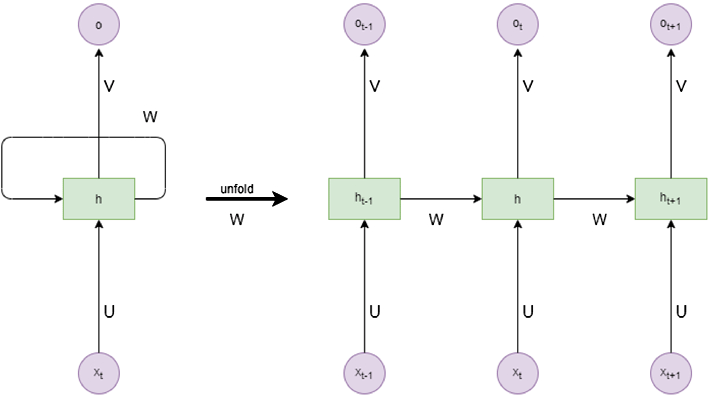
\includegraphics[width=0.9\textwidth]{rnn_unrolled.png}
    \captionof{figure}{Kiến trúc của một RNN. Bên trái là dạng nén với vòng lặp. Bên phải là dạng "trải ra theo thời gian" (unrolled), cho thấy cách trạng thái ẩn $h$ được truyền từ bước này sang bước tiếp theo.}
    \label{fig:rnn_unrolled}
\end{center}

\subsubsection{Kiến trúc và Dòng chảy Dữ liệu}
Tại mỗi bước thời gian $t$:
\begin{enumerate}
    \item \textbf{Đầu vào:} Vector từ $x_t$ và trạng thái ẩn từ bước trước $h_{t-1}$.
    \item \textbf{Tính toán trạng thái ẩn mới:} Trạng thái ẩn mới, $h_t$, được tính bằng cách kết hợp $x_t$ và $h_{t-1}$ qua một phép biến đổi tuyến tính và một hàm kích hoạt (thường là `tanh`).
        \begin{equation}
            h_t = \tanh(W_{hh} h_{t-1} + W_{xh} x_t + b_h)
        \end{equation}
        Trong đó, $W_{hh}$ và $W_{xh}$ là các ma trận trọng số được \textbf{chia sẻ (shared)} trên tất cả các bước thời gian. Đây là điểm mấu chốt: mô hình học một bộ quy tắc duy nhất để cập nhật trí nhớ, bất kể vị trí trong chuỗi.
    \item \textbf{Tạo đầu ra (tùy chọn):} Một đầu ra $y_t$ có thể được tạo ra từ trạng thái ẩn $h_t$.
        \begin{equation}
            y_t = W_{hy} h_t + b_y
        \end{equation}
\end{enumerate}
\begin{tcolorbox}[
    title=Ghi chú sâu về Thiết kế của RNN Đơn giản,
    colback=green!5!white, colframe=green!50!black, fonttitle=\bfseries
]
\textbf{1. Tại sao phải Chia sẻ Trọng số?} \\
Đây là nguyên lý nền tảng của RNN. Việc sử dụng cùng một bộ trọng số ($W_{hh}, W_{xh}$) ở mọi bước thời gian cho phép mô hình học một quy tắc cập nhật \textbf{tổng quát} có thể áp dụng cho bất kỳ vị trí nào trong chuỗi. Nếu mỗi bước thời gian có một bộ trọng số riêng, mô hình sẽ:
\begin{itemize}
    \item Có số lượng tham số khổng lồ, phụ thuộc vào độ dài chuỗi, khiến việc huấn luyện bất khả thi.
    \item Không thể tổng quát hóa cho các chuỗi có độ dài khác với dữ liệu huấn luyện. Nó sẽ chỉ học thuộc lòng các mẫu ở các vị trí cố định.
\end{itemize}
Việc chia sẻ trọng số chính là cách RNN học được một "thuật toán" xử lý chuỗi.

\textbf{2. Tại sao dùng hàm `tanh`?} \\
Hàm `tanh` đưa đầu ra về khoảng $[-1, 1]$. Điều này giúp giữ cho các giá trị trong trạng thái ẩn không bị tăng hoặc giảm quá nhanh, tức là kiểm soát dòng chảy thông tin một cách tương đối ổn định. Nếu dùng `ReLU` (vốn không có giới hạn trên), trạng thái ẩn có thể tăng lên vô hạn, làm cho vấn đề bùng nổ gradient trở nên trầm trọng hơn rất nhiều. `tanh` hoạt động như một cơ chế "bão hòa" tự nhiên.
\end{tcolorbox}

\subsubsection{Huấn luyện RNN: Lan truyền ngược theo thời gian (BPTT)}
\label{sssec:bptt}
Quá trình huấn luyện một RNN cũng dựa trên việc tối thiểu hóa một hàm mất mát, nhưng có một sự phức tạp hơn so với mạng FNN.
\begin{itemize}
    \item \textbf{Hàm Mất mát:} Tại mỗi bước thời gian $t$, mô hình tạo ra một dự đoán $y_t$. Lỗi tại bước đó, $\mathcal{L}_t$, được tính toán bằng cách so sánh $y_t$ với nhãn thật tương ứng. \textbf{Tổng lỗi} cho toàn bộ chuỗi là tổng của các lỗi tại mỗi bước: $\mathcal{L} = \sum_{t=1}^{T} \mathcal{L}_t$.
    
    \item \textbf{Lan truyền ngược theo thời gian (Backpropagation Through Time - BPTT):} Để tính toán gradient của tổng lỗi $\mathcal{L}$ theo các trọng số (ví dụ $W_{hh}$), chúng ta phải sử dụng một biến thể của backpropagation gọi là BPTT. Gradient tại một bước thời gian $t$ không chỉ phụ thuộc vào lỗi tại bước $t$, mà còn phụ thuộc vào gradient từ tất cả các bước thời gian \textit{trong tương lai} ($t+1, t+2, \dots, T$) được truyền ngược lại thông qua trạng thái ẩn $h$.
    
    \item \textbf{Vấn đề của BPTT:} Chính việc gradient phải được truyền ngược qua nhiều bước thời gian này là nguyên nhân gây ra các vấn đề nan giải được thảo luận dưới đây.
\end{itemize}

\subsubsection{Vấn đề nan giải: Vanishing và Exploding Gradients}
RNN về lý thuyết có thể học các phụ thuộc tầm xa. Tuy nhiên, trong thực tế, chúng gặp rất nhiều khó khăn. Quá trình huấn luyện RNN sử dụng thuật toán lan truyền ngược theo thời gian (Backpropagation Through Time - BPTT). Khi lan truyền gradient lỗi ngược qua nhiều bước thời gian, gradient này phải đi qua phép nhân lặp đi lặp lại với ma trận trọng số $W_{hh}$.

\begin{itemize}
    \item \textbf{Vanishing Gradients (Triệt tiêu Gradient):} Nếu các giá trị trong $W_{hh}$ nhỏ (norm < 1), sau nhiều lần nhân, gradient sẽ co lại và tiến dần về 0.
        \begin{itemize}
            \item \textbf{Hậu quả:} Mạng không thể học được các phụ thuộc giữa các từ ở xa nhau. Tín hiệu lỗi từ tương lai không thể lan truyền đủ xa về quá khứ để cập nhật trọng số một cách có ý nghĩa. RNN trở nên "thiển cận", chỉ nhớ được vài bước gần nhất. Đây là vấn đề nghiêm trọng nhất.
        \end{itemize}
    \item \textbf{Exploding Gradients (Bùng nổ Gradient):} Nếu các giá trị trong $W_{hh}$ lớn (norm > 1), gradient sẽ tăng theo cấp số nhân và trở nên khổng lồ.
        \begin{itemize}
            \item \textbf{Hậu quả:} Gây ra các bước cập nhật trọng số cực lớn, làm cho quá trình huấn luyện trở nên mất ổn định. Vấn đề này có thể được giải quyết phần nào bằng kỹ thuật \textit{gradient clipping} (cắt bớt gradient nếu nó vượt quá một ngưỡng).
        \end{itemize}
\end{itemize}

Vấn đề triệt tiêu gradient đã thúc đẩy sự ra đời của các kiến trúc RNN phức tạp hơn, có khả năng kiểm soát dòng chảy thông tin một cách thông minh hơn.

\subsection{Long Short-Term Memory (LSTM)}
\label{ssec:lstm}
LSTM, được giới thiệu bởi Hochreiter \& Schmidhuber vào năm 1997 \cite{hochreiter1997long}, là một biến thể đặc biệt của RNN, được thiết kế một cách xuất sắc để giải quyết vấn đề triệt tiêu gradient. Nó đã trở thành kiến trúc thống trị cho các bài toán chuỗi trong gần hai thập kỷ.

\subsubsection{Tư duy cốt lõi: Các Cổng và Trạng thái Ô nhớ}
Ý tưởng thiên tài của LSTM là giới thiệu một "làn đường cao tốc" cho thông tin, gọi là \textbf{trạng thái ô nhớ (cell state)}, ký hiệu là $C_t$. Trạng thái ô nhớ này chạy dọc theo toàn bộ chuỗi, chỉ với một vài tương tác tuyến tính nhỏ. Thông tin có thể dễ dàng chảy trên làn đường này mà không bị thay đổi nhiều.

LSTM có khả năng thêm hoặc bớt thông tin ra khỏi trạng thái ô nhớ một cách cẩn thận, được điều khiển bởi các cấu trúc gọi là \textbf{cổng (gates)}. Cổng là một cách để thông tin có thể đi qua một cách tùy chọn. Chúng bao gồm một lớp mạng sigmoid và một phép nhân theo từng phần tử (element-wise multiplication).

\begin{center}
    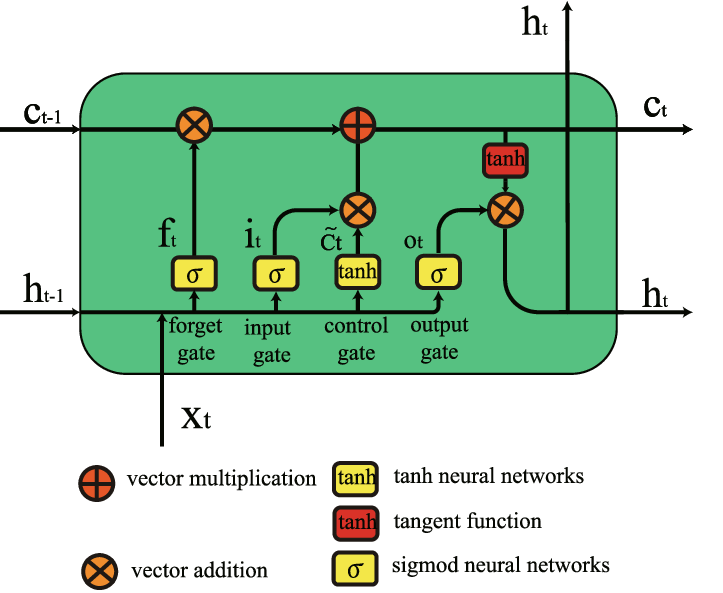
\includegraphics[width=0.7\textwidth]{lstm_cell_diagram.png}
    \captionof{figure}{Sơ đồ chi tiết của một ô nhớ LSTM. Nó bao gồm 3 cổng chính (Quên, Nạp, Xuất) và một trạng thái ô nhớ $C_t$ chạy ngang.}
    \label{fig:lstm_cell_diagram}
\end{center}

Một ô LSTM có ba cổng để bảo vệ và kiểm soát trạng thái ô nhớ:

\paragraph{1. Cổng Quên (Forget Gate - $f_t$)}
Cổng này quyết định xem thông tin nào nên được \textbf{loại bỏ} khỏi trạng thái ô nhớ của bước trước.
$$ f_t = \sigma(W_f [h_{t-1}, x_t] + b_f) $$
Nó nhìn vào $h_{t-1}$ và $x_t$, và xuất ra một vector số từ 0 đến 1 cho mỗi số trong trạng thái ô nhớ $C_{t-1}$. Số 1 có nghĩa là "giữ lại hoàn toàn", số 0 có nghĩa là "quên hoàn toàn".

\paragraph{2. Cổng Nạp (Input Gate - $i_t$)}
Cổng này quyết định xem thông tin mới nào nên được \textbf{lưu trữ} vào trạng thái ô nhớ. Quá trình này có hai bước:
\begin{enumerate}
    \item Một lớp sigmoid (cổng nạp) quyết định những giá trị nào chúng ta sẽ cập nhật.
        $$ i_t = \sigma(W_i [h_{t-1}, x_t] + b_i) $$
    \item Một lớp `tanh` tạo ra một vector các giá trị ứng viên mới, $\tilde{C}_t$, có thể được thêm vào trạng thái.
        $$ \tilde{C}_t = \tanh(W_C [h_{t-1}, x_t] + b_C) $$
\end{enumerate}

\paragraph{3. Cập nhật Trạng thái Ô nhớ}
Bây giờ, chúng ta cập nhật trạng thái ô nhớ cũ $C_{t-1}$ thành trạng thái mới $C_t$.
$$ C_t = f_t \odot C_{t-1} + i_t \odot \tilde{C}_t $$
Ký hiệu $\odot$ là phép nhân theo từng phần tử. Chúng ta nhân trạng thái cũ với $f_t$ (quên đi những gì đã quyết định quên), sau đó cộng với $i_t \odot \tilde{C}_t$ (thêm vào những thông tin mới đã quyết định nạp). Phép cộng này chính là chìa khóa giúp gradient có thể chảy ngược một cách dễ dàng, giải quyết vấn đề triệt tiêu gradient.

\paragraph{4. Cổng Xuất (Output Gate - $o_t$)}
Cuối cùng, cổng này quyết định xem chúng ta sẽ xuất ra cái gì. Đầu ra này sẽ dựa trên trạng thái ô nhớ của chúng ta, nhưng sẽ là một phiên bản đã được "lọc".
\begin{enumerate}
    \item Một lớp sigmoid quyết định phần nào của trạng thái ô nhớ chúng ta sẽ xuất ra.
        $$ o_t = \sigma(W_o [h_{t-1}, x_t] + b_o) $$
    \item Chúng ta đưa trạng thái ô nhớ qua hàm `tanh` (để đưa giá trị về khoảng [-1, 1]) và nhân nó với đầu ra của cổng sigmoid, để chỉ xuất ra những phần chúng ta muốn.
        $$ h_t = o_t \odot \tanh(C_t) $$
\end{enumerate}
Trạng thái ẩn mới $h_t$ này sẽ được sử dụng để dự đoán đầu ra $y_t$ và được truyền tới bước thời gian tiếp theo.
\paragraph{Phân tích: Tại sao LSTM hoạt động?}
Sự kỳ diệu của LSTM nằm ở cách nó tách biệt dòng chảy thông tin và kiểm soát nó một cách tinh vi:
\begin{itemize}
    \item \textbf{Con đường cao tốc Gradient (Gradient Highway):} Nhìn lại công thức cập nhật trạng thái ô nhớ: $C_t = f_t \odot C_{t-1} + i_t \odot \tilde{C}_t$. Thành phần quan trọng nhất là phép cộng. Trong quá trình lan truyền ngược, gradient của $C_t$ đối với $C_{t-1}$ có một thành phần trực tiếp là $f_t$. Do $f_t$ được điều khiển bởi hàm sigmoid, giá trị của nó thường không bị quá nhỏ hoặc quá lớn. Điều này tạo ra một "con đường" gần như không bị cản trở để gradient có thể chảy ngược qua nhiều bước thời gian mà không bị triệt tiêu hoàn toàn. RNN đơn giản chỉ có phép nhân lặp đi lặp lại, khiến gradient dễ dàng biến mất.
    
    \item \textbf{Phân vai Trí nhớ:} LSTM tạo ra một sự phân vai rõ ràng:
        \begin{itemize}
            \item \textbf{Trạng thái Ô nhớ ($C_t$):} Đóng vai trò như \textbf{trí nhớ dài hạn}. Nó chứa tất cả thông tin tích lũy được. Nó có thể được thay đổi một cách cẩn trọng thông qua các cổng, nhưng bản chất là một "kho lưu trữ".
            \item \textbf{Trạng thái Ẩn ($h_t$):} Đóng vai trò như \textbf{trí nhớ làm việc (working memory)}. Nó là một phiên bản "đã lọc" của trí nhớ dài hạn, chỉ chứa những thông tin liên quan đến quyết định cần đưa ra \textit{tại thời điểm hiện tại}. Việc tách biệt này cho phép mô hình vừa lưu trữ thông tin từ rất xa trong quá khứ ($C_t$), vừa tập trung vào những gì cần thiết cho bước tiếp theo ($h_t$).
        \end{itemize}
\end{itemize}
\subsection{Gated Recurrent Unit (GRU)}
\label{ssec:gru}
Được giới thiệu bởi Cho và các cộng sự vào năm 2014, GRU \cite{cho2014learning} là một biến thể của LSTM với kiến trúc đơn giản hơn. Nó kết hợp cổng quên và cổng nạp thành một "cổng cập nhật" duy nhất, và cũng hợp nhất trạng thái ô nhớ và trạng thái ẩn.

\paragraph{Tư duy cốt lõi}
GRU giữ lại tinh thần của LSTM là sử dụng các cổng để điều khiển dòng chảy thông tin, nhưng với ít tham số hơn, giúp việc huấn luyện nhanh hơn và hiệu quả hơn trên các bộ dữ liệu nhỏ.

GRU có hai cổng chính:
\paragraph{1. Cổng Cập nhật (Update Gate - $z_t$)}
Cổng này có vai trò tương tự cả cổng quên và cổng nạp trong LSTM. Nó quyết định xem bao nhiêu thông tin từ trạng thái ẩn quá khứ ($h_{t-1}$) nên được giữ lại, và bao nhiêu thông tin mới ($\tilde{h}_t$) nên được thêm vào.
$$ z_t = \sigma(W_z [h_{t-1}, x_t] + b_z) $$

\paragraph{2. Cổng Reset (Reset Gate - $r_t$)}
Cổng này quyết định xem bao nhiêu phần của trạng thái ẩn quá khứ nên được "quên" đi khi tính toán trạng thái ứng viên mới.
$$ r_t = \sigma(W_r [h_{t-1}, x_t] + b_r) $$

\paragraph{Tính toán Trạng thái}
\begin{enumerate}
    \item Trạng thái ẩn ứng viên mới $\tilde{h}_t$ được tính toán, nhưng có sử dụng cổng reset để kiểm soát ảnh hưởng của $h_{t-1}$.
        $$ \tilde{h}_t = \tanh(W_h [r_t \odot h_{t-1}, x_t] + b_h) $$
        Nếu cổng reset $r_t$ gần bằng 0, mô hình sẽ gần như bỏ qua hoàn toàn thông tin quá khứ và chỉ tập trung vào đầu vào hiện tại $x_t$ để tạo trạng thái mới.
    \item Trạng thái ẩn cuối cùng $h_t$ là một sự nội suy tuyến tính giữa trạng thái cũ $h_{t-1}$ và trạng thái ứng viên mới $\tilde{h}_t$, được điều khiển bởi cổng cập nhật $z_t$.
        $$ h_t = (1 - z_t) \odot h_{t-1} + z_t \odot \tilde{h}_t $$
\end{enumerate}
\paragraph{Phân tích: Sự đánh đổi của GRU}
GRU là một ví dụ tuyệt vời về việc đơn giản hóa kiến trúc mà vẫn giữ được hiệu quả cốt lõi.
\begin{itemize}
    \item \textbf{Cổng Reset - Cơ chế "Khởi động lại Ngữ cảnh":} Cổng reset ($r_t$) cho phép GRU bỏ qua hoàn toàn trí nhớ quá khứ khi cần thiết. Hãy tưởng tượng khi đọc một đoạn văn và gặp một dấu chấm hết câu, bắt đầu một câu mới với chủ đề khác. Cổng reset có thể học cách "kích hoạt" (đưa giá trị về gần 0) tại những điểm chuyển tiếp này, cho phép trạng thái ứng viên mới $\tilde{h}_t$ được hình thành chủ yếu từ đầu vào hiện tại $x_t$, tạo ra một khởi đầu mới cho ngữ cảnh.
    
    \item \textbf{Cổng Cập nhật - Nội suy mượt mà:} Công thức $h_t = (1 - z_t) \odot h_{t-1} + z_t \odot \tilde{h}_t$ hoạt động như một bộ điều khiển "rò rỉ". Khi $z_t$ gần bằng 0, phần lớn $h_{t-1}$ sẽ được sao chép trực tiếp sang $h_t$, giúp thông tin được bảo tồn qua các bước thời gian dài. Ngược lại, khi $z_t$ gần bằng 1, thông tin mới sẽ được ưu tiên. Sự cân bằng này giúp GRU mô hình hóa các phụ thuộc dài hạn một cách hiệu quả, dù không có một "trạng thái ô nhớ" riêng biệt.
\end{itemize}
Việc gộp trạng thái ô nhớ và trạng thái ẩn làm cho GRU mất đi một chút sức mạnh biểu diễn so với LSTM, nhưng chính sự đơn giản này lại giúp nó huấn luyện nhanh hơn và đôi khi tổng quát hóa tốt hơn trên các tập dữ liệu nhỏ.
\begin{tcolorbox}[
    title=So sánh LSTM và GRU,
    colback=green!5!white, colframe=green!60!black, fonttitle=\bfseries
]
\begin{tabular}{p{0.45\linewidth} | p{0.45\linewidth}}
    \textbf{LSTM} & \textbf{GRU} \\
    \hline
    Có 3 cổng: Quên, Nạp, Xuất. & Có 2 cổng: Cập nhật, Reset. \\
    \hline
    Có trạng thái ô nhớ ($C_t$) và trạng thái ẩn ($h_t$) riêng biệt. & Chỉ có một trạng thái ẩn ($h_t$). \\
    \hline
    Nhiều tham số hơn. & Ít tham số hơn. \\
    \hline
    Linh hoạt và mạnh mẽ hơn về mặt lý thuyết. & Nhanh hơn, hiệu quả hơn về mặt tính toán và cần ít dữ liệu hơn để tổng quát hóa. \\
    \hline
    \textbf{Khi nào dùng?} Không có quy tắc tuyệt đối. GRU là một lựa chọn khởi đầu tốt. Nếu bài toán rất phức tạp và có đủ dữ liệu, LSTM có thể cho hiệu năng nhỉnh hơn.
\end{tabular}
\end{tcolorbox}
% % !TEX root = ../main.tex
% File: chapters_part1/chap3_4.tex
% Nội dung cho Phần 3.4: Seq2Seq và Attention

\section{Mô hình Chuỗi-sang-Chuỗi (Seq2Seq) và Cơ chế Chú ý (Attention)}
\label{sec:seq2seq_attention}

Kiến trúc RNN, LSTM, hay GRU mà chúng ta vừa học có một hạn chế cơ bản: chúng được thiết kế để xử lý các bài toán có đầu vào là một chuỗi và đầu ra là một giá trị duy nhất (phân loại) hoặc một chuỗi có độ dài bằng với chuỗi đầu vào (gán nhãn chuỗi).

Nhưng điều gì sẽ xảy ra với các bài toán như \textbf{dịch máy} (một câu tiếng Việt có 10 từ có thể được dịch thành một câu tiếng Anh 8 từ) hoặc \textbf{tóm tắt văn bản} (một văn bản 1000 từ được tóm tắt thành một câu 20 từ)? Ở những bài toán này, độ dài chuỗi đầu vào và đầu ra là khác nhau và không có sự tương ứng 1-1.

Mô hình Chuỗi-sang-Chuỗi (Sequence-to-Sequence - Seq2Seq) ra đời để giải quyết chính xác vấn đề này.

\subsection{Kiến trúc Encoder-Decoder của Seq2Seq}
\label{ssec:encoder_decoder}
Seq2Seq, được giới thiệu gần như đồng thời bởi Sutskever và các cộng sự (2014) \cite{sutskever2014sequence} và Cho và các cộng sự (2014) \cite{cho2014learning}, dựa trên một kiến trúc thanh lịch gồm hai thành phần chính: \textbf{Bộ mã hóa (Encoder)} và \textbf{Bộ giải mã (Decoder)}.

\begin{center}
    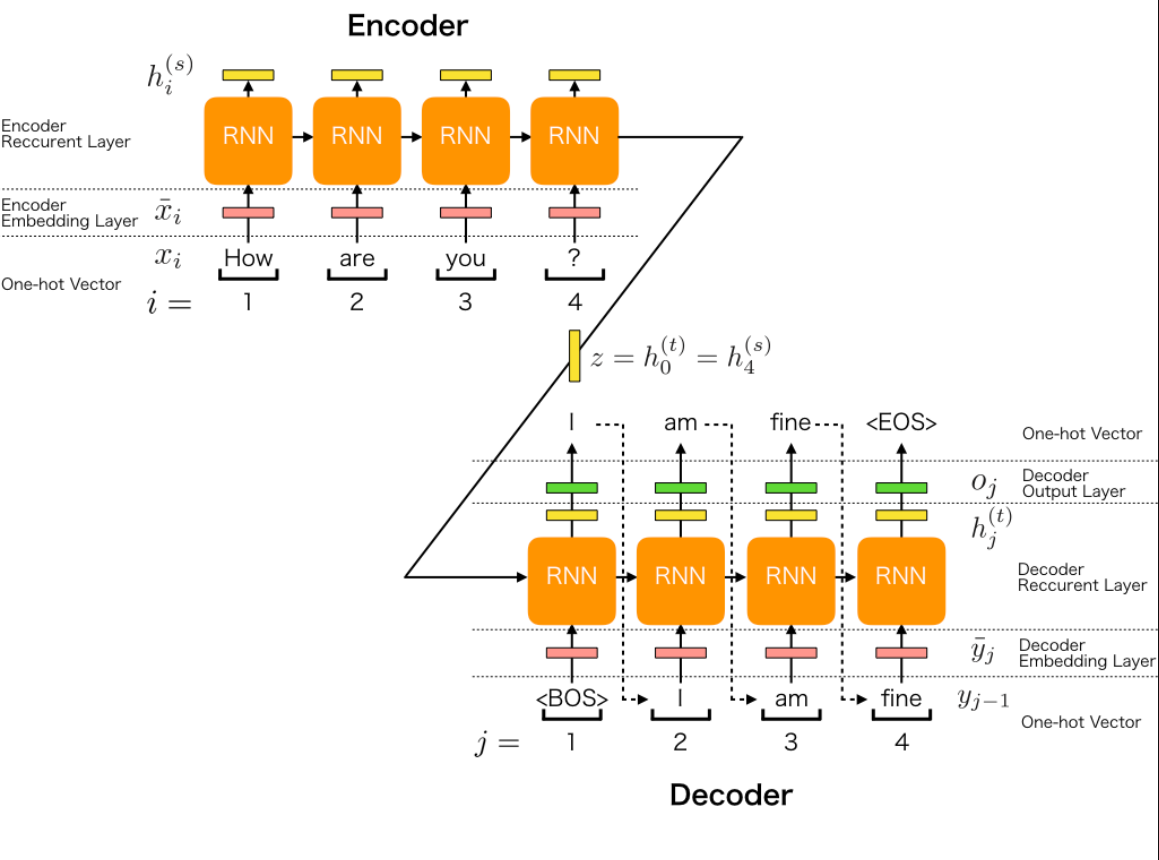
\includegraphics[width=0.9\textwidth]{seq2seq_architecture.png}
    \captionof{figure}{Kiến trúc Encoder-Decoder tổng quát. Encoder "đọc" và nén chuỗi đầu vào thành một vector ngữ cảnh. Decoder sử dụng vector này để "viết" ra chuỗi đầu ra.}
    \label{fig:seq2seq_architecture}
\end{center}

\subsubsection{Bộ mã hóa (The Encoder)}
\paragraph{Nhiệm vụ}
Nhiệm vụ của Encoder là "đọc" toàn bộ chuỗi đầu vào (ví dụ, một câu tiếng Việt) và nén toàn bộ thông tin, ngữ nghĩa của nó vào một vector có kích thước cố định. Vector này được gọi là \textbf{vector ngữ cảnh (context vector)} hay "thought vector".

\paragraph{Cấu tạo và Hoạt động}
\begin{itemize}
    \item Encoder thường là một mạng RNN (hoặc LSTM, GRU).
    \item Nó nhận đầu vào là một chuỗi các vector từ (word embeddings) của câu nguồn, ví dụ: $x_1, x_2, \dots, x_T$.
    \item Nó xử lý chuỗi này tuần tự, từng từ một. Tại mỗi bước, nó cập nhật trạng thái ẩn của mình.
    \item Điều quan trọng là chúng ta \textbf{bỏ qua tất cả các đầu ra (outputs) của Encoder ở mỗi bước}. Chúng ta chỉ quan tâm đến \textbf{trạng thái ẩn cuối cùng ($h_T$)}. Trạng thái ẩn cuối cùng này chính là vector ngữ cảnh, vì nó được cho là đã tóm tắt thông tin của toàn bộ chuỗi đầu vào.
\end{itemize}
\begin{tcolorbox}[
    title=Ghi chú sâu về Thiết kế của Encoder,
    colback=green!5!white, colframe=green!50!black, fonttitle=\bfseries
]
\textbf{1. Tại sao Encoder thường là Mạng RNN Hai chiều (Bi-RNN)?} \\
Một RNN đơn giản xử lý câu từ trái sang phải. Trạng thái ẩn $h_t$ tại từ $x_t$ chỉ chứa thông tin về các từ từ $x_1$ đến $x_t$. Điều này là một hạn chế, vì ngữ nghĩa của một từ thường phụ thuộc vào cả ngữ cảnh đứng trước và đứng sau nó.
\begin{itemize}
    \item \textbf{Bi-RNN} giải quyết vấn đề này bằng cách sử dụng hai RNN riêng biệt: một RNN chạy xuôi (forward) từ đầu đến cuối câu, và một RNN chạy ngược (backward) từ cuối về đầu.
    \item Tại mỗi từ $x_t$, biểu diễn cuối cùng của nó là sự \textbf{kết hợp} (thường là nối - concatenation) của trạng thái ẩn từ cả hai chiều: $\overrightarrow{h_t}$ và $\overleftarrow{h_t}$.
    \item Vector ngữ cảnh cuối cùng cho mô hình Seq2Seq cơ bản sẽ là nối của trạng thái ẩn cuối cùng của RNN xuôi ($\overrightarrow{h_T}$) và trạng thái ẩn cuối cùng của RNN ngược ($\overleftarrow{h_1}$).
\end{itemize}
Việc này cung cấp một biểu diễn ngữ cảnh phong phú hơn nhiều cho mỗi từ, và đã trở thành tiêu chuẩn trong hầu hết các mô hình Encoder-Decoder.

\textbf{2. Tại sao không dùng Pooling thay vì trạng thái ẩn cuối cùng?} \\
Sử dụng trạng thái ẩn cuối cùng là cách đơn giản nhất, nhưng nó có thể bị ảnh hưởng bởi "hiệu ứng gần đây" (recency bias) - các từ cuối chuỗi có thể có ảnh hưởng lớn hơn. Các phương pháp khác như:
\begin{itemize}
    \item \textbf{Average/Max Pooling:} Lấy trung bình hoặc giá trị lớn nhất trên tất cả các trạng thái ẩn (của Bi-RNN). Cách này dân chủ hơn, đảm bảo mọi từ đều có đóng góp, nhưng có thể làm "lu mờ" các chi tiết quan trọng.
\end{itemize}
Trong thực tế, trước khi Attention ra đời, không có phương pháp nào là hoàn hảo. Sự ra đời của Attention đã giải quyết triệt để vấn đề này bằng cách cho phép Decoder tự quyết định nên tập trung vào đâu, thay vì ép Encoder phải tạo ra một bản tóm tắt duy nhất.
\end{tcolorbox}
\subsubsection{Bộ giải mã (The Decoder)}
\paragraph{Nhiệm vụ}
Nhiệm vụ của Decoder là lấy vector ngữ cảnh do Encoder cung cấp và "giải nén" nó để sinh ra chuỗi đầu ra (ví dụ, câu tiếng Anh tương ứng), từng từ một.

\paragraph{Cấu tạo và Hoạt động}
\begin{itemize}
    \item Decoder cũng là một mạng RNN (hoặc LSTM, GRU) khác, thường có kiến trúc tương tự Encoder nhưng với bộ trọng số riêng.
    \item \textbf{Khởi tạo:} Trạng thái ẩn ban đầu của Decoder ($h_0^{dec}$) được khởi tạo bằng chính vector ngữ cảnh (trạng thái ẩn cuối cùng của Encoder, $h_T^{enc}$). Đây là "cây cầu" duy nhất kết nối Encoder và Decoder.
    \item \textbf{Quá trình sinh từ (Generation):} Quá trình này diễn ra tuần tự:
        \begin{enumerate}
            \item \textbf{Bước 1:} Decoder nhận vào một token bắt đầu đặc biệt (ví dụ: `<SOS>` - Start of Sentence) và trạng thái ẩn ban đầu. Nó tính toán trạng thái ẩn mới $h_1^{dec}$ và tạo ra một phân phối xác suất trên toàn bộ từ vựng của ngôn ngữ đích thông qua một lớp softmax. Từ có xác suất cao nhất được chọn làm từ đầu ra đầu tiên, $y_1$.
            \item \textbf{Bước 2:} Từ vừa được sinh ra, $y_1$, sẽ trở thành \textbf{đầu vào cho bước tiếp theo}. Decoder nhận $y_1$ và trạng thái ẩn $h_1^{dec}$ để tính $h_2^{dec}$ và sinh ra từ tiếp theo $y_2$.
            \item Quá trình này lặp đi lặp lại (mang tính \textbf{tự hồi quy - auto-regressive}) cho đến khi Decoder sinh ra một token kết thúc đặc biệt (`<EOS>` - End of Sentence).
        \end{enumerate}
\end{itemize}

\subsubsection{Vấn đề của cái "Cổ chai" (The Bottleneck Problem)}
Kiến trúc Encoder-Decoder cơ bản này rất thông minh, nhưng nó có một điểm yếu chết người: nó buộc Encoder phải nén toàn bộ thông tin của một câu, dù dài và phức tạp đến đâu, vào một \textbf{vector ngữ cảnh có kích thước cố định}.
\begin{itemize}
    \item Đây là một "cổ chai" thông tin. Với những câu dài, việc nhồi nhét tất cả các chi tiết ngữ nghĩa vào một vector duy nhất là cực kỳ khó khăn, nếu không muốn nói là bất khả thi.
    \item Decoder chỉ được "nhìn" vào bản tóm tắt này một lần duy nhất lúc bắt đầu. Nó không có cách nào để quay lại và xem xét các phần cụ thể của câu nguồn khi nó đang dịch.
\end{itemize}
Hãy tưởng tượng bạn yêu cầu một dịch giả nghe toàn bộ một bài phát biểu dài, sau đó phải dịch lại toàn bộ từ trí nhớ mà không được ghi chép. Đó chính là những gì mô hình Seq2Seq cơ bản phải làm. Hạn chế này đã dẫn đến sự ra đời của ý tưởng có sức ảnh hưởng bậc nhất trong lịch sử NLP hiện đại: \textbf{Cơ chế Chú ý (Attention)}.

\subsubsection{Huấn luyện mô hình Seq2Seq}
Mục tiêu huấn luyện của mô hình Seq2Seq là tối đa hóa xác suất của chuỗi đầu ra đúng ($Y = y_1, ..., y_{T'}$) khi biết chuỗi đầu vào ($X = x_1, ..., x_T$). Điều này tương đương với việc tối thiểu hóa hàm mất mát \textbf{Cross-Entropy} trên toàn bộ chuỗi đầu ra:
$$ \mathcal{L}(\theta) = - \sum_{t=1}^{T'} \log P(y_t | y_1, ..., y_{t-1}, c) $$
trong đó $c$ là vector ngữ cảnh từ Encoder. Trong quá trình huấn luyện, lỗi tại mỗi bước của Decoder được tính toán và lan truyền ngược qua cả Decoder và Encoder để cập nhật tất cả các trọng số. Kỹ thuật \textbf{Teacher Forcing} được sử dụng để làm cho quá trình này ổn định và hiệu quả hơn.

\subsubsection{Huấn luyện và Suy luận: Teacher Forcing và Beam Search}
Có hai kỹ thuật quan trọng liên quan đến cách mô hình Seq2Seq được huấn luyện và sử dụng để sinh văn bản.

\paragraph{Huấn luyện với Teacher Forcing}
Trong quá trình huấn luyện, tại mỗi bước $t$, thay vì đưa từ mà Decoder vừa dự đoán ở bước $t-1$ vào làm đầu vào, chúng ta lại đưa từ \textbf{chính xác (ground truth)} trong chuỗi đích vào.
\begin{itemize}
    \item \textbf{Ưu điểm:} Kỹ thuật này giúp quá trình huấn luyện ổn định và hội tụ nhanh hơn rất nhiều. Nó ngăn ngừa việc lỗi bị tích tụ: nếu mô hình dự đoán sai ở bước đầu, lỗi sai đó sẽ không làm ảnh hưởng đến các bước sau trong cùng một chuỗi huấn luyện. Mỗi bước thời gian được coi là một mẫu huấn luyện độc lập.
    \item \textbf{Nhược điểm:} Nó tạo ra một sự khác biệt giữa lúc huấn luyện và lúc suy luận (khi mô hình không có "thầy" để chỉ bảo). Điều này có thể dẫn đến hiệu năng kém khi mô hình phải tự sinh ra một chuỗi dài.
\end{itemize}

\paragraph{Suy luận với Beam Search}
Trong lúc suy luận, việc luôn chọn từ có xác suất cao nhất tại mỗi bước (gọi là \textbf{Greedy Search}) thường không tạo ra được câu tốt nhất. Một lựa chọn có vẻ tốt ở hiện tại có thể dẫn đến một ngõ cụt. \textbf{Beam Search} là một giải pháp cân bằng.
\begin{itemize}
    \item Thay vì chỉ giữ lại 1 ứng viên tốt nhất ở mỗi bước, Beam Search sẽ giữ lại $k$ ứng viên (gọi là \textit{beam width} hoặc \textit{kích thước beam}) có xác suất chuỗi cao nhất.
    \item Tại bước tiếp theo, nó sẽ mở rộng mỗi ứng viên trong beam với tất cả các từ khả dĩ trong từ vựng, tính toán xác suất của các chuỗi mới, và lại chọn ra $k$ chuỗi tốt nhất để tiếp tục.
    \item Quá trình này là một sự đánh đổi giữa chất lượng và chi phí tính toán. Nó hiệu quả hơn nhiều so với Greedy Search và là kỹ thuật tiêu chuẩn để sinh văn bản trong các mô hình Seq2Seq.
\end{itemize}
\subsection{Cơ chế Chú ý (Attention Mechanism)}
\label{ssec:attention}

\subsubsection{Trực giác cốt lõi: Dịch như con người}
Khi một dịch giả con người dịch một câu, họ không làm như mô hình Seq2Seq cơ bản. Khi dịch một từ, họ sẽ tập trung (pay attention) vào một hoặc một vài từ liên quan trong câu gốc. Cơ chế Chú ý được thiết kế để mô phỏng chính xác hành vi này.

\begin{tcolorbox}[
    title=Ý tưởng đột phá của Attention,
    colback=yellow!10!white, colframe=yellow!50!black, fonttitle=\bfseries
]
Thay vì ép Encoder tạo ra một vector ngữ cảnh duy nhất, hãy cho phép Decoder, tại \textbf{mỗi bước} sinh từ của mình, có khả năng \textbf{"nhìn lại" toàn bộ chuỗi đầu vào} và quyết định xem phần nào của chuỗi đầu vào là quan trọng nhất cần phải "chú ý" đến ngay tại thời điểm đó.
\end{tcolorbox}

Attention tạo ra một "đường tắt" kết nối trực tiếp Decoder với tất cả các trạng thái ẩn của Encoder, phá vỡ cái "cổ chai" thông tin.

\subsubsection{Cơ chế hoạt động chi tiết}
Cơ chế chú ý được tích hợp vào giữa Encoder và Decoder. Thay vì chỉ truyền trạng thái ẩn cuối cùng, Encoder sẽ cung cấp \textbf{tất cả các trạng thái ẩn của nó} ($h_1^{enc}, h_2^{enc}, \dots, h_T^{enc}$) cho Decoder.

Bây giờ, tại mỗi bước $t$ của Decoder, để sinh ra từ $y_t$, nó sẽ thực hiện các bước sau:

\begin{center}
    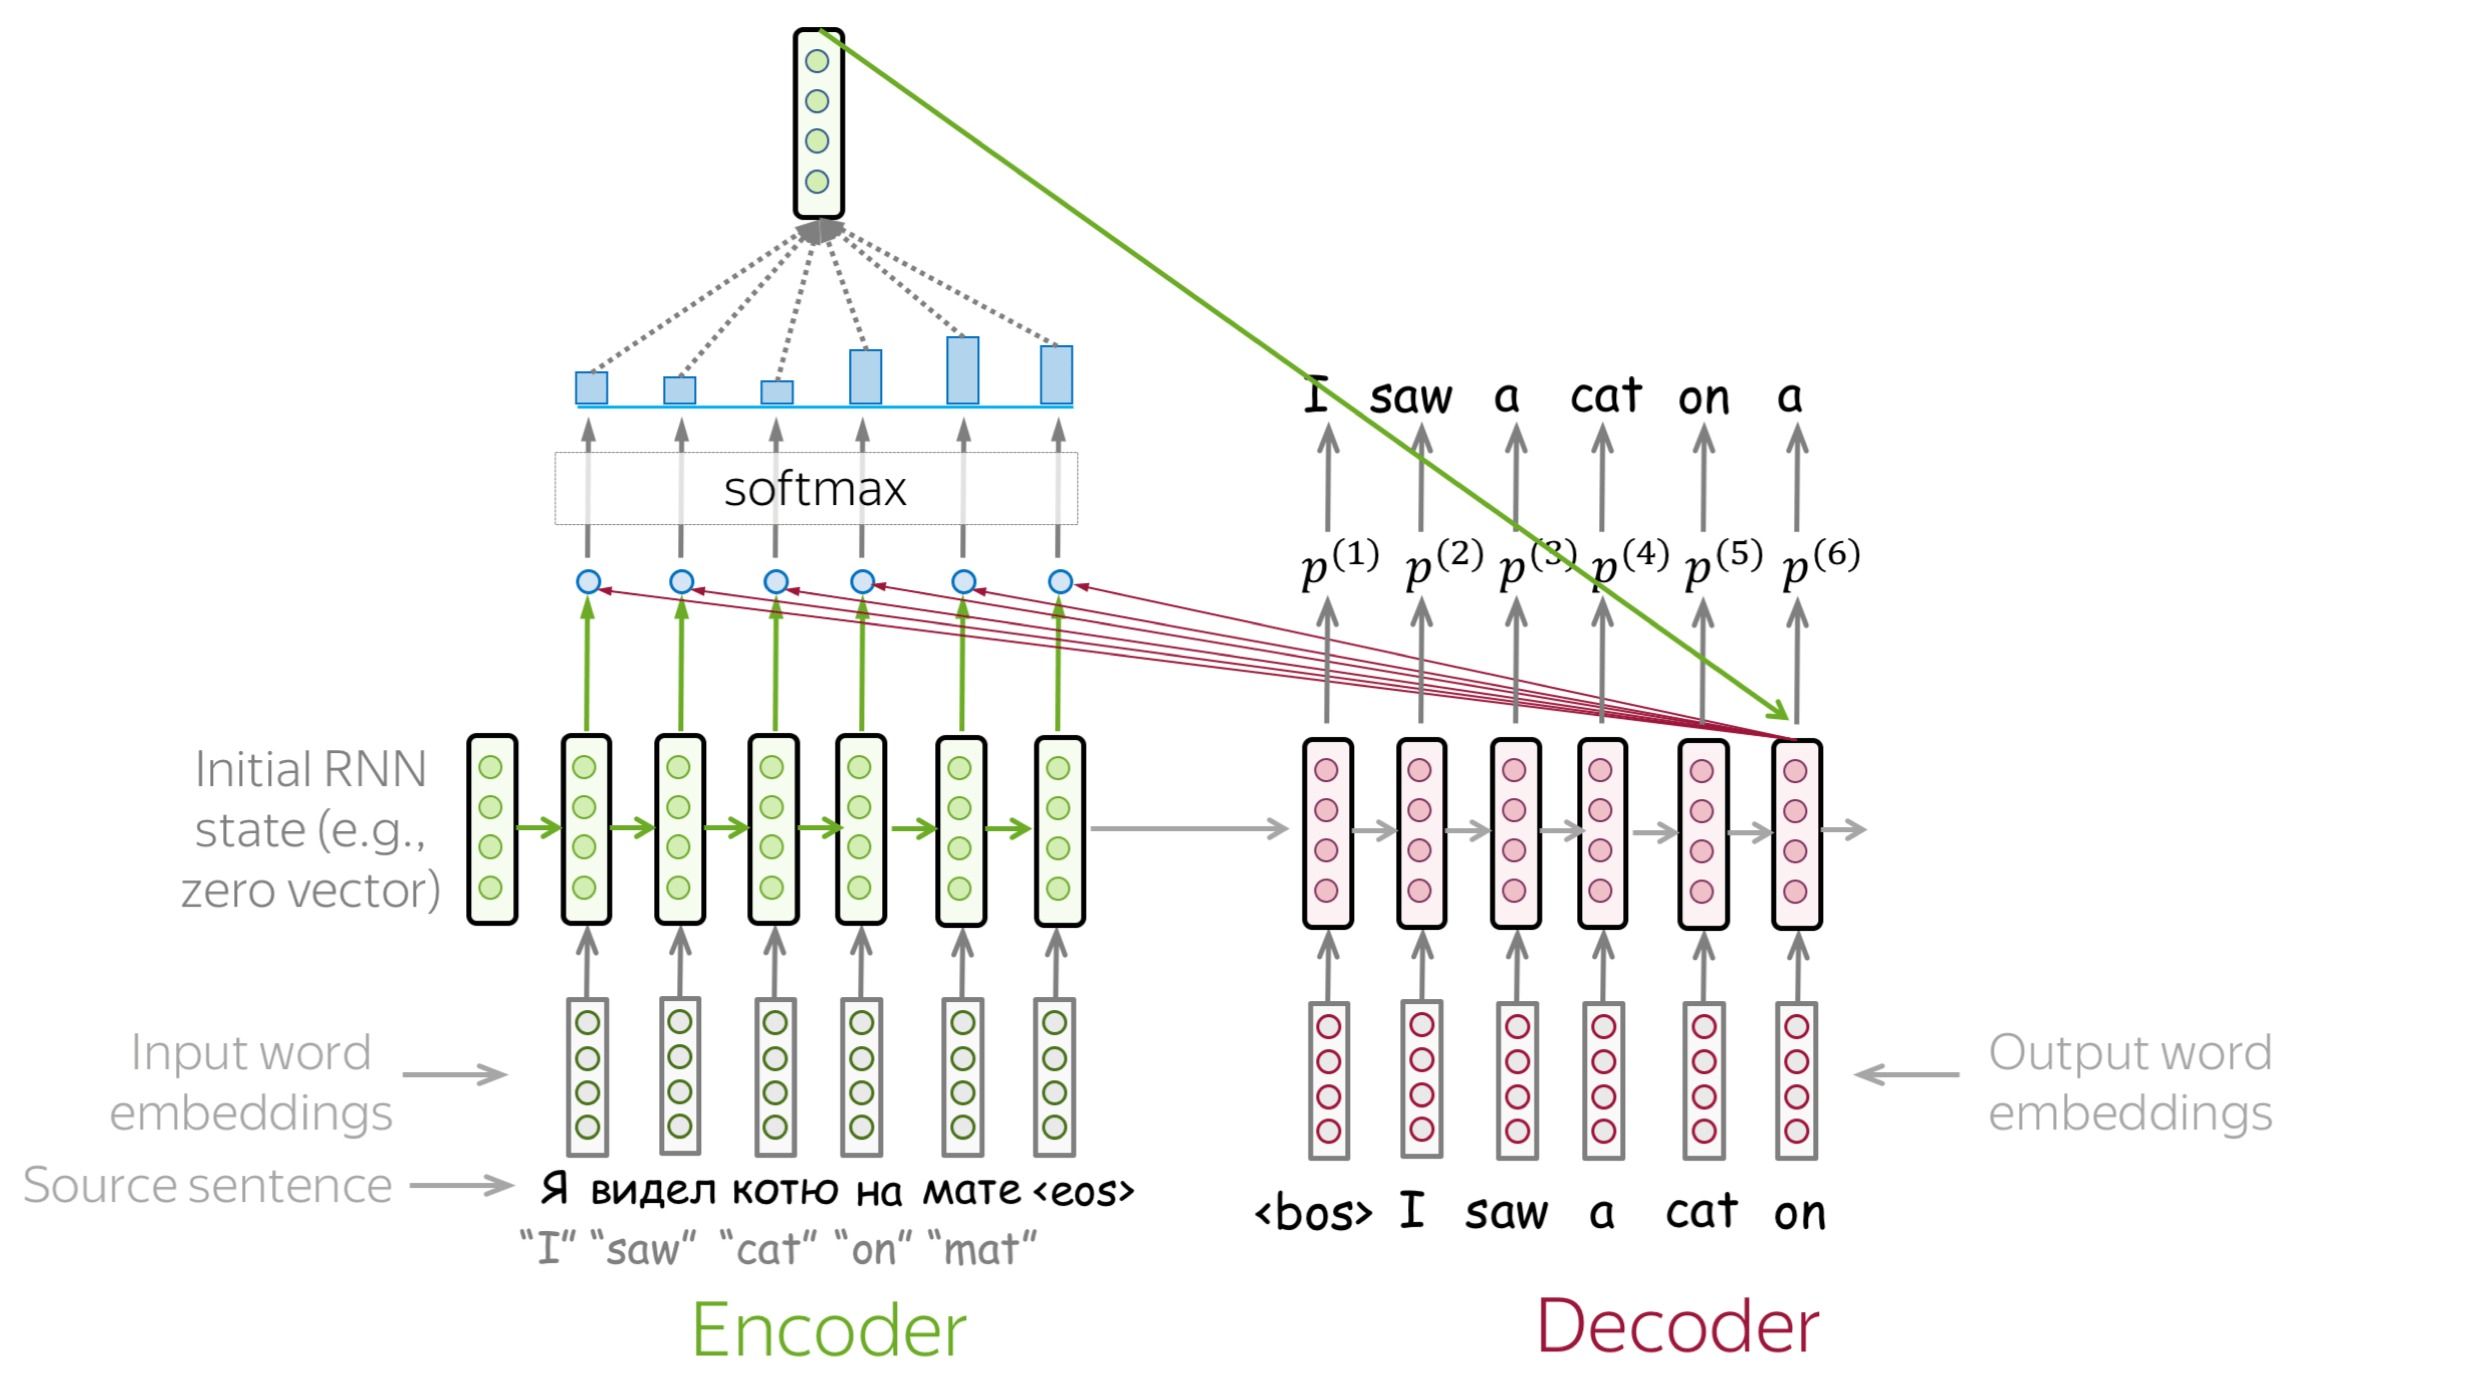
\includegraphics[width=1.0\textwidth]{seq2seq_attention_mechanism.png}
    \captionof{figure}{Cơ chế Chú ý trong Seq2Seq. Tại bước sinh từ thứ $t$ của Decoder, nó tính toán các trọng số chú ý ($\alpha_t$) để tạo ra một vector ngữ cảnh động ($c_t$) từ tất cả các trạng thái ẩn của Encoder.}
    \label{fig:seq2seq_attention_mechanism}
\end{center}

\paragraph{Bước 1: Tính điểm chú ý (Attention Scores)}
Decoder lấy trạng thái ẩn của nó ở bước trước, $h_{t-1}^{dec}$, và so sánh nó với \textbf{từng trạng thái ẩn của Encoder}, $h_i^{enc}$, để tính ra một "điểm số tương hợp" (alignment score). Điểm số này đo lường mức độ "liên quan" của từ đầu vào thứ $i$ đối với việc sinh ra từ đầu ra thứ $t$. Có nhiều cách để định nghĩa hàm $\text{score}(h_{t-1}^{dec}, h_i^{enc})$, trong đó phổ biến là:
\begin{itemize}
    \item \textbf{Additive Attention (\cite{bahdanau2014neural}):} Sử dụng một mạng nơ-ron nhỏ truyền thẳng (feed-forward) có một lớp ẩn. Cách này mạnh mẽ và linh hoạt.
        $$ \text{score}(h_{t-1}^{dec}, h_i^{enc}) = v_a^T \tanh(W_a [h_{t-1}^{dec}; h_i^{enc}]) $$
    \item \textbf{Dot-Product Attention (\cite{luong2015effective}):} Đơn giản là lấy tích vô hướng giữa hai vector. Cách này rất nhanh và hiệu quả về mặt tính toán, nhưng yêu cầu số chiều của $h^{dec}$ và $h^{enc}$ phải bằng nhau.
        $$ \text{score}(h_{t-1}^{dec}, h_i^{enc}) = (h_{t-1}^{dec})^T h_i^{enc} $$
    \item \textbf{Scaled Dot-Product Attention:} Một biến thể của Dot-Product, được giới thiệu trong bài báo Transformer \cite{vaswani2017attention}. Nó chia tích vô hướng cho căn bậc hai của số chiều vector ($\sqrt{d_k}$) để tránh gradient quá nhỏ khi số chiều lớn.
\end{itemize}
Sự lựa chọn hàm score ảnh hưởng đến độ phức tạp tính toán và hiệu năng của mô hình. Dot-Product và các biến thể của nó đã trở nên rất phổ biến do hiệu quả của chúng, đặc biệt là trong kiến trúc Transformer.
\paragraph{Bước 2: Chuẩn hóa thành trọng số (Softmax)}
Các điểm số vừa tính được sẽ được đưa qua một hàm \textbf{softmax}. Điều này biến các điểm số thành một phân phối xác suất, gọi là \textbf{trọng số chú ý (attention weights)}, ký hiệu là $\alpha_{ti}$.
$$ \alpha_{ti} = \frac{\exp(\text{score}(h_{t-1}^{dec}, h_i^{enc}))}{\sum_{j=1}^{T} \exp(\text{score}(h_{t-1}^{dec}, h_j^{enc}))} $$
Tổng của tất cả các trọng số $\alpha_{ti}$ (với $i$ từ 1 đến $T$) bằng 1. Mỗi $\alpha_{ti}$ cho biết "mức độ chú ý" mà Decoder nên dành cho từ đầu vào thứ $i$ khi sinh ra từ đầu ra thứ $t$.

\paragraph{Bước 3: Tính toán vector ngữ cảnh động (Context Vector)}
Vector ngữ cảnh $c_t$ bây giờ không còn cố định nữa. Nó là một \textbf{tổng có trọng số (weighted sum)} của tất cả các trạng thái ẩn của Encoder, với các trọng số chính là các trọng số chú ý vừa tính được.
$$ c_t = \sum_{i=1}^{T} \alpha_{ti} h_i^{enc} $$
Vector ngữ cảnh $c_t$ này được tính toán lại ở \textbf{mỗi bước của Decoder}. Nếu các trọng số chú ý $\alpha_{ti}$ tập trung vào trạng thái ẩn thứ $j$ của Encoder, thì vector $c_t$ sẽ chủ yếu chứa thông tin từ $h_j^{enc}$.

\paragraph{Bước 4: Sử dụng vector ngữ cảnh để dự đoán}
Cuối cùng, vector ngữ cảnh động $c_t$ được nối với trạng thái ẩn của Decoder ở bước trước, $h_{t-1}^{dec}$, và được đưa vào làm đầu vào cho lớp RNN của Decoder để tính ra trạng thái ẩn hiện tại $h_t^{dec}$.
$$ h_t^{dec} = \text{RNN}_{\text{dec}}(h_{t-1}^{dec}, c_t) $$
Trạng thái $h_t^{dec}$ này sau đó được dùng để dự đoán từ đầu ra $y_t$. Một cách khác là nối $c_t$ với $h_t^{dec}$ trước khi đưa vào lớp softmax cuối cùng.

\subsubsection{Sức mạnh của Attention}
\begin{itemize}
    \item \textbf{Phá vỡ nút thắt cổ chai:} Thông tin không còn bị nén vào một vector duy nhất. Decoder có quyền truy cập vào toàn bộ chuỗi đầu vào ở mọi thời điểm.
    \item \textbf{Khả năng diễn giải (Interpretability):} Chúng ta có thể trực quan hóa ma trận trọng số chú ý để xem mô hình đang "nhìn" vào đâu khi dịch. Ví dụ, khi dịch từ "bạn", mô hình sẽ có trọng số chú ý cao nhất ở từ "you". Điều này giúp gỡ lỗi và hiểu mô hình tốt hơn.
    \item \textbf{Hiệu năng vượt trội:} Các mô hình Seq2Seq với Attention đã ngay lập tức thiết lập một tiêu chuẩn mới về chất lượng cho dịch máy và nhiều bài toán chuỗi-sang-chuỗi khác, vượt xa các hệ thống thống kê trước đó.
\end{itemize}

Cơ chế Chú ý không chỉ là một cải tiến. Nó là một trong những ý tưởng nền tảng và có sức ảnh hưởng lớn nhất trong lịch sử học sâu, là tiền đề trực tiếp cho sự ra đời của kiến trúc Transformer mà chúng ta sẽ tìm hiểu ở chương tiếp theo.
% % !TEX root = ../../main.tex
% File: part2/chapters3/chap3_5.tex

\section{Vòng đời MLOps cho LLM}
\label{sec:llmops_lifecycle}
Triển khai mô hình không phải là điểm kết thúc. Để một ứng dụng AI thành công trong dài hạn, nó cần phải được giám sát, bảo trì, và cải tiến liên tục. Đây là vòng đời MLOps.

\subsection{Giám sát mô hình (Model Monitoring)}
\label{ssec:model_monitoring}
Sau khi triển khai, chúng ta cần theo dõi hai loại vấn đề chính:

\paragraph{1. Giám sát Hệ thống (System Monitoring)}
\begin{itemize}
    \item \textbf{Mục tiêu:} Đảm bảo dịch vụ API đang hoạt động ổn định.
    \item \textbf{Các metric cần theo dõi:}
        \begin{itemize}
            \item \textbf{Độ trễ (Latency):} Thời gian để xử lý một yêu cầu.
            \item \textbf{Thông lượng (Throughput):} Số lượng yêu cầu được xử lý mỗi giây.
            \item \textbf{Tỷ lệ lỗi (Error Rate):} Tỷ lệ các yêu cầu trả về lỗi (ví dụ: HTTP 500).
            \item \textbf{Sử dụng tài nguyên:} Mức sử dụng CPU, GPU, RAM.
        \end{itemize}
\end{itemize}

\paragraph{2. Giám sát Chất lượng Mô hình (Model Quality Monitoring)}
\begin{itemize}
    \item \textbf{Mục tiêu:} Đảm bảo mô hình vẫn đang đưa ra các dự đoán tốt trong thế giới thực.
    \item \textbf{Thách thức:} Chúng ta thường không có "nhãn thật" ngay lập tức để so sánh.
    \item \textbf{Phát hiện Trôi dạt Dữ liệu (Data Drift):}
        \begin{itemize}
            \item \textbf{Vấn đề:} Phân phối của dữ liệu trong môi trường production (live data) bắt đầu khác biệt so với phân phối của dữ liệu đã được dùng để huấn luyện mô hình. Ví dụ, một mô hình phân tích cảm xúc được huấn luyện trên các bình luận về phim ảnh có thể hoạt động kém đi khi người dùng bắt đầu bình luận về các sự kiện chính trị.
            \item \textbf{Cách phát hiện:} So sánh các thuộc tính thống kê giữa dữ liệu live và dữ liệu huấn luyện. Đối với văn bản, chúng ta có thể so sánh \textbf{phân phối của các vector embedding}. Nếu embedding của dữ liệu live bắt đầu trôi dạt ra xa khỏi embedding của dữ liệu huấn luyện, đó là một dấu hiệu mạnh mẽ của data drift.
        \end{itemize}
    \item \textbf{Phát hiện Trôi dạt Khái niệm (Concept Drift):}
        \begin{itemize}
            \item \textbf{Vấn đề:} Mối quan hệ giữa đầu vào và đầu ra thay đổi. Ví dụ, ý nghĩa của từ "corona" đã thay đổi hoàn toàn sau năm 2020.
            \item \textbf{Cách phát hiện:} Thường khó phát hiện hơn và yêu cầu phải có một luồng phản hồi từ người dùng hoặc gán nhãn lại một phần dữ liệu live.
        \end{itemize}
\end{itemize}

\subsection{Quy trình Tái huấn luyện và Cập nhật Mô hình}
\label{ssec:retraining_pipeline}
Khi việc giám sát cho thấy hiệu năng của mô hình đang suy giảm, chúng ta cần một quy trình để cập nhật nó.
\begin{itemize}
    \item \textbf{Thu thập Dữ liệu mới và Phản hồi:} Thiết lập một "vòng lặp phản hồi" (feedback loop) để thu thập dữ liệu mới từ môi trường production, đặc biệt là các trường hợp mà mô hình dự đoán sai.
    \item \textbf{Gán nhãn lại (Re-labeling):} Gán nhãn cho bộ dữ liệu mới này.
    \item \textbf{Tái huấn luyện (Re-training):} Huấn luyện lại mô hình trên một bộ dữ liệu kết hợp giữa dữ liệu cũ và dữ liệu mới.
    \item \textbf{Đánh giá và So sánh:} Đánh giá mô hình mới trên một tập kiểm tra được giữ riêng. Chỉ triển khai mô hình mới nếu nó thực sự hoạt động tốt hơn mô hình cũ.
    \item \textbf{Triển khai theo chiến lược an toàn:}
        \begin{itemize}
            \item \textbf{Shadow Deployment:} Triển khai mô hình mới song song với mô hình cũ, chỉ để ghi lại dự đoán của nó mà không ảnh hưởng đến người dùng, nhằm so sánh hiệu năng.
            \item \textbf{Canary Release / A/B Testing:} Dần dần chuyển một phần nhỏ traffic của người dùng sang mô hình mới và theo dõi chặt chẽ các metric kinh doanh trước khi chuyển toàn bộ.
        \end{itemize}
\end{itemize}
Vòng đời MLOps này biến việc phát triển mô hình từ một dự án một lần thành một quy trình liên tục, đảm bảo rằng ứng dụng AI của bạn luôn được cải tiến và thích ứng với thế giới đang thay đổi.

\bigskip
\hrule
\bigskip

\begin{center}
    \textbf{\Large KẾT THÚC CHƯƠNG 3}
\end{center}
\textit{Chương 3 đã đưa chúng ta vào hành trình từ một mô hình đã được huấn luyện đến một dịch vụ AI hoàn chỉnh, hoạt động trong môi trường production. Chúng ta đã học cách tối ưu hóa, đóng gói, phục vụ và giám sát các mô hình ngôn ngữ lớn. Việc trang bị các kỹ năng MLOps này là cực kỳ quan trọng, đảm bảo rằng các sản phẩm AI không chỉ thông minh mà còn mạnh mẽ, có khả năng mở rộng và bền vững. Giờ đây, bạn đã sẵn sàng để kết hợp tất cả các kiến thức đã học và áp dụng chúng vào việc xây dựng các ứng dụng cụ thể trong chương cuối cùng của giáo trình.}

% \chapter{CÁC KIẾN TRÚC MẠNG NƠ-RON KINH ĐIỂN}
\label{chap:deep_learning_architectures}

Chào mừng bạn đến với kỷ nguyên học sâu của NLP. Trong chương 2, chúng ta đã thấy các mô hình thống kê như N-gram có thể nắm bắt các phụ thuộc cục bộ, nhưng lại bất lực trước các mối quan hệ tầm xa. Cuộc cách mạng word embedding đã cho chúng ta các vector từ mang đầy ngữ nghĩa, nhưng làm thế nào để kết hợp chúng lại nhằm hiểu được ý nghĩa của cả một câu hay một đoạn văn?

Chương này sẽ giới thiệu các kiến trúc mạng nơ-ron nền tảng được thiết kế đặc biệt để xử lý dữ liệu dạng chuỗi như ngôn ngữ tự nhiên. Những kiến trúc này không chỉ đơn thuần "nhìn" vào các từ một cách riêng lẻ, mà còn có khả năng "ghi nhớ" và "lý luận" dựa trên thông tin đã xử lý trước đó, cho phép chúng nắm bắt được ngữ cảnh và các phụ thuộc phức tạp trong câu.
% % !TEX root = ../main.tex
% File: chapters_part1/chap4_1.tex
% Nội dung cho Chương 4, Phần 1

\section{Kiến trúc Transformer Gốc ("Attention Is All You Need")}
\label{sec:vanilla_transformer}

Để hiểu được sức mạnh của Transformer, chúng ta cần mổ xẻ từng khối xây dựng nên nó, bắt đầu từ ý tưởng cốt lõi nhất: Self-Attention.

\subsection{Chi tiết cơ chế Self-Attention: Scaled Dot-Product và Multi-Head Attention}
\label{ssec:self_attention}

Cơ chế chú ý mà chúng ta đã học trong mô hình Seq2Seq (ở mục \ref{sec:seq2seq_attention}) là \textit{cross-attention}, nơi Decoder "chú ý" đến Encoder. \textbf{Self-Attention (Tự chú ý)} là một biến thể đặc biệt, nơi một chuỗi "chú ý" đến chính nó.

\paragraph{Tư duy cốt lõi}
Self-Attention cho phép mỗi từ trong một câu có thể "nhìn" vào tất cả các từ khác trong cùng một câu để tính toán ra một biểu diễn mới cho chính nó. Biểu diễn mới này không chỉ chứa thông tin của bản thân từ đó, mà còn được "làm giàu" bởi ngữ cảnh từ các từ liên quan nhất.

Ví dụ, trong câu "Con mèo không muốn băng qua đường vì nó quá mệt", khi xử lý từ "nó", Self-Attention sẽ giúp mô hình xác định rằng "nó" có liên quan mật thiết đến "mèo" chứ không phải "đường", và tạo ra một biểu diễn cho "nó" mang nhiều thông tin của "mèo".

\subsubsection{Scaled Dot-Product Attention}
Đây là khối xây dựng cơ bản của Self-Attention trong Transformer. Nó hoạt động dựa trên ba khái niệm được lấy cảm hứng từ các hệ thống tìm kiếm thông tin: \textbf{Query, Key, và Value}.

\begin{tcolorbox}[
    title={Trực giác về Query, Key, Value},
    colback=yellow!10!white, colframe=yellow!50!black, fonttitle=\bfseries
]
Hãy tưởng tượng bạn đang tìm kiếm video trên YouTube.
\begin{itemize}
    \item \textbf{Query (Truy vấn):} Là cụm từ bạn gõ vào thanh tìm kiếm (ví dụ: "công thức nấu phở"). Nó đại diện cho \textit{thông tin bạn đang cần}.
    \item \textbf{Key (Khóa):} Mỗi video trên YouTube có một bộ các từ khóa (tiêu đề, mô tả) để mô tả nội dung của nó. Nó đại diện cho \textit{thông tin mà một đối tượng có thể cung cấp}.
    \item \textbf{Value (Giá trị):} Chính là nội dung của video. Nó đại diện cho \textit{thông tin thực sự sẽ được lấy ra}.
\end{itemize}
Cơ chế hoạt động là: bạn lấy \textbf{Query} của mình, so sánh nó với \textbf{Key} của tất cả các video để tìm ra các video liên quan nhất (tính điểm tương đồng). Sau đó, bạn lấy một "tổng có trọng số" của các \textbf{Value} (nội dung video), trong đó các video liên quan hơn sẽ có trọng số cao hơn.
\end{tcolorbox}

\begin{tcolorbox}[
    title={Tại sao lại cần đến ba vai trò Q, K, V?},
    colback=green!5!white, colframe=green!50!black, fonttitle=\bfseries
]
Một câu hỏi tự nhiên là: Tại sao mỗi từ đầu vào $x_i$ lại cần được chiếu thành ba vector $q_i, k_i, v_i$ riêng biệt? Tại sao không chỉ dùng chính các $x_i$?
\begin{itemize}
    \item \textbf{Sự linh hoạt:} Việc tách thành ba vai trò mang lại sự linh hoạt tối đa. Nó cho phép mô hình học cách so sánh các từ dựa trên một loại đặc trưng (được mã hóa trong $Q$ và $K$) và sau đó trích xuất một loại đặc trưng khác (được mã hóa trong $V$).
    \item \textbf{Ví dụ trực quan:} Hãy quay lại ví dụ "Con mèo... vì nó quá mệt".
        \begin{itemize}
            \item Khi tính toán biểu diễn cho "nó", \textbf{Query ($q_{\text{nó}}$)} có thể mã hóa thông tin: "Tôi là một đại từ, tôi cần tìm một danh từ làm tham chiếu".
            \item \textbf{Key ($k_{\text{mèo}}$)} của "mèo" có thể mã hóa: "Tôi là một danh từ giống đực/cái, số ít". Key này sẽ "khớp" rất tốt với Query của "nó".
            \item \textbf{Value ($v_{\text{mèo}}$)} của "mèo" có thể chứa thông tin ngữ nghĩa thực sự của từ: "một loài động vật bốn chân".
        \end{itemize}
        Sau khi $q_{\text{nó}}$ khớp với $k_{\text{mèo}}$, biểu diễn mới của "nó" sẽ nhận được một phần lớn thông tin từ $v_{\text{mèo}}$, giúp nó "hiểu" rằng nó đang nói về một con vật. Nếu chỉ dùng $x_i$ cho cả ba vai trò, mô hình sẽ bị hạn chế trong việc học các mối quan hệ phức tạp như vậy.
\end{itemize}
\end{tcolorbox}

Trong Self-Attention, mỗi từ đầu vào sẽ đóng cả ba vai trò này.
\paragraph{Cơ chế hoạt động chi tiết}
Giả sử chúng ta có một chuỗi các vector đầu vào $X = (x_1, x_2, \dots, x_n)$.
\begin{enumerate}
    \item \textbf{Tạo Query, Key, Value:} Chúng ta tạo ra ba ma trận trọng số có thể học được: $W^Q, W^K, W^V$. Mỗi vector đầu vào $x_i$ sẽ được nhân với ba ma trận này để tạo ra ba vector tương ứng:
        \begin{itemize}
            \item $q_i = W^Q x_i$ (Query vector của từ $i$)
            \item $k_i = W^K x_i$ (Key vector của từ $i$)
            \item $v_i = W^V x_i$ (Value vector của từ $i$)
        \end{itemize}
        Toàn bộ chuỗi sẽ tạo ra các ma trận $Q, K, V$.
    \item \textbf{Tính điểm chú ý (Attention Scores):} Để tính toán biểu diễn mới cho từ thứ $i$, chúng ta lấy Query của nó ($q_i$) và tính tích vô hướng (dot product) với Key của \textit{tất cả} các từ khác (bao gồm cả chính nó), $k_j$. Đây chính là bước so sánh "Query" với tất cả các "Key".
        $$ \text{score}(i, j) = q_i \cdot k_j $$
    \item \textbf{Chia tỷ lệ (Scaling):} Tích vô hướng có thể tạo ra các giá trị rất lớn, đẩy hàm softmax vào vùng có gradient rất nhỏ, gây khó khăn cho việc huấn luyện. Bài báo đã "scale" (chia) các điểm số này cho căn bậc hai của số chiều của vector Key, $d_k$.
        $$ \text{scaled\_score}(i, j) = \frac{q_i \cdot k_j}{\sqrt{d_k}} $$
    \item \textbf{Chuẩn hóa (Softmax):} Áp dụng hàm softmax trên các điểm số đã chia tỷ lệ để có được các trọng số chú ý $\alpha_{ij}$.
    \item \textbf{Tính toán đầu ra:} Biểu diễn đầu ra mới cho từ $i$, ký hiệu là $z_i$, được tính bằng tổng có trọng số của \textit{tất cả} các vector Value.
        $$ z_i = \sum_{j=1}^{n} \alpha_{ij} v_j $$
\end{enumerate}

Toàn bộ quá trình này có thể được tóm gọn trong một công thức ma trận duy nhất, cực kỳ hiệu quả cho việc tính toán trên GPU:
\begin{equation}
    \text{Attention}(Q, K, V) = \text{softmax}\left(\frac{QK^T}{\sqrt{d_k}}\right)V
    \label{eq:scaled_dot_product_attention}
\end{equation}

\begin{center}
    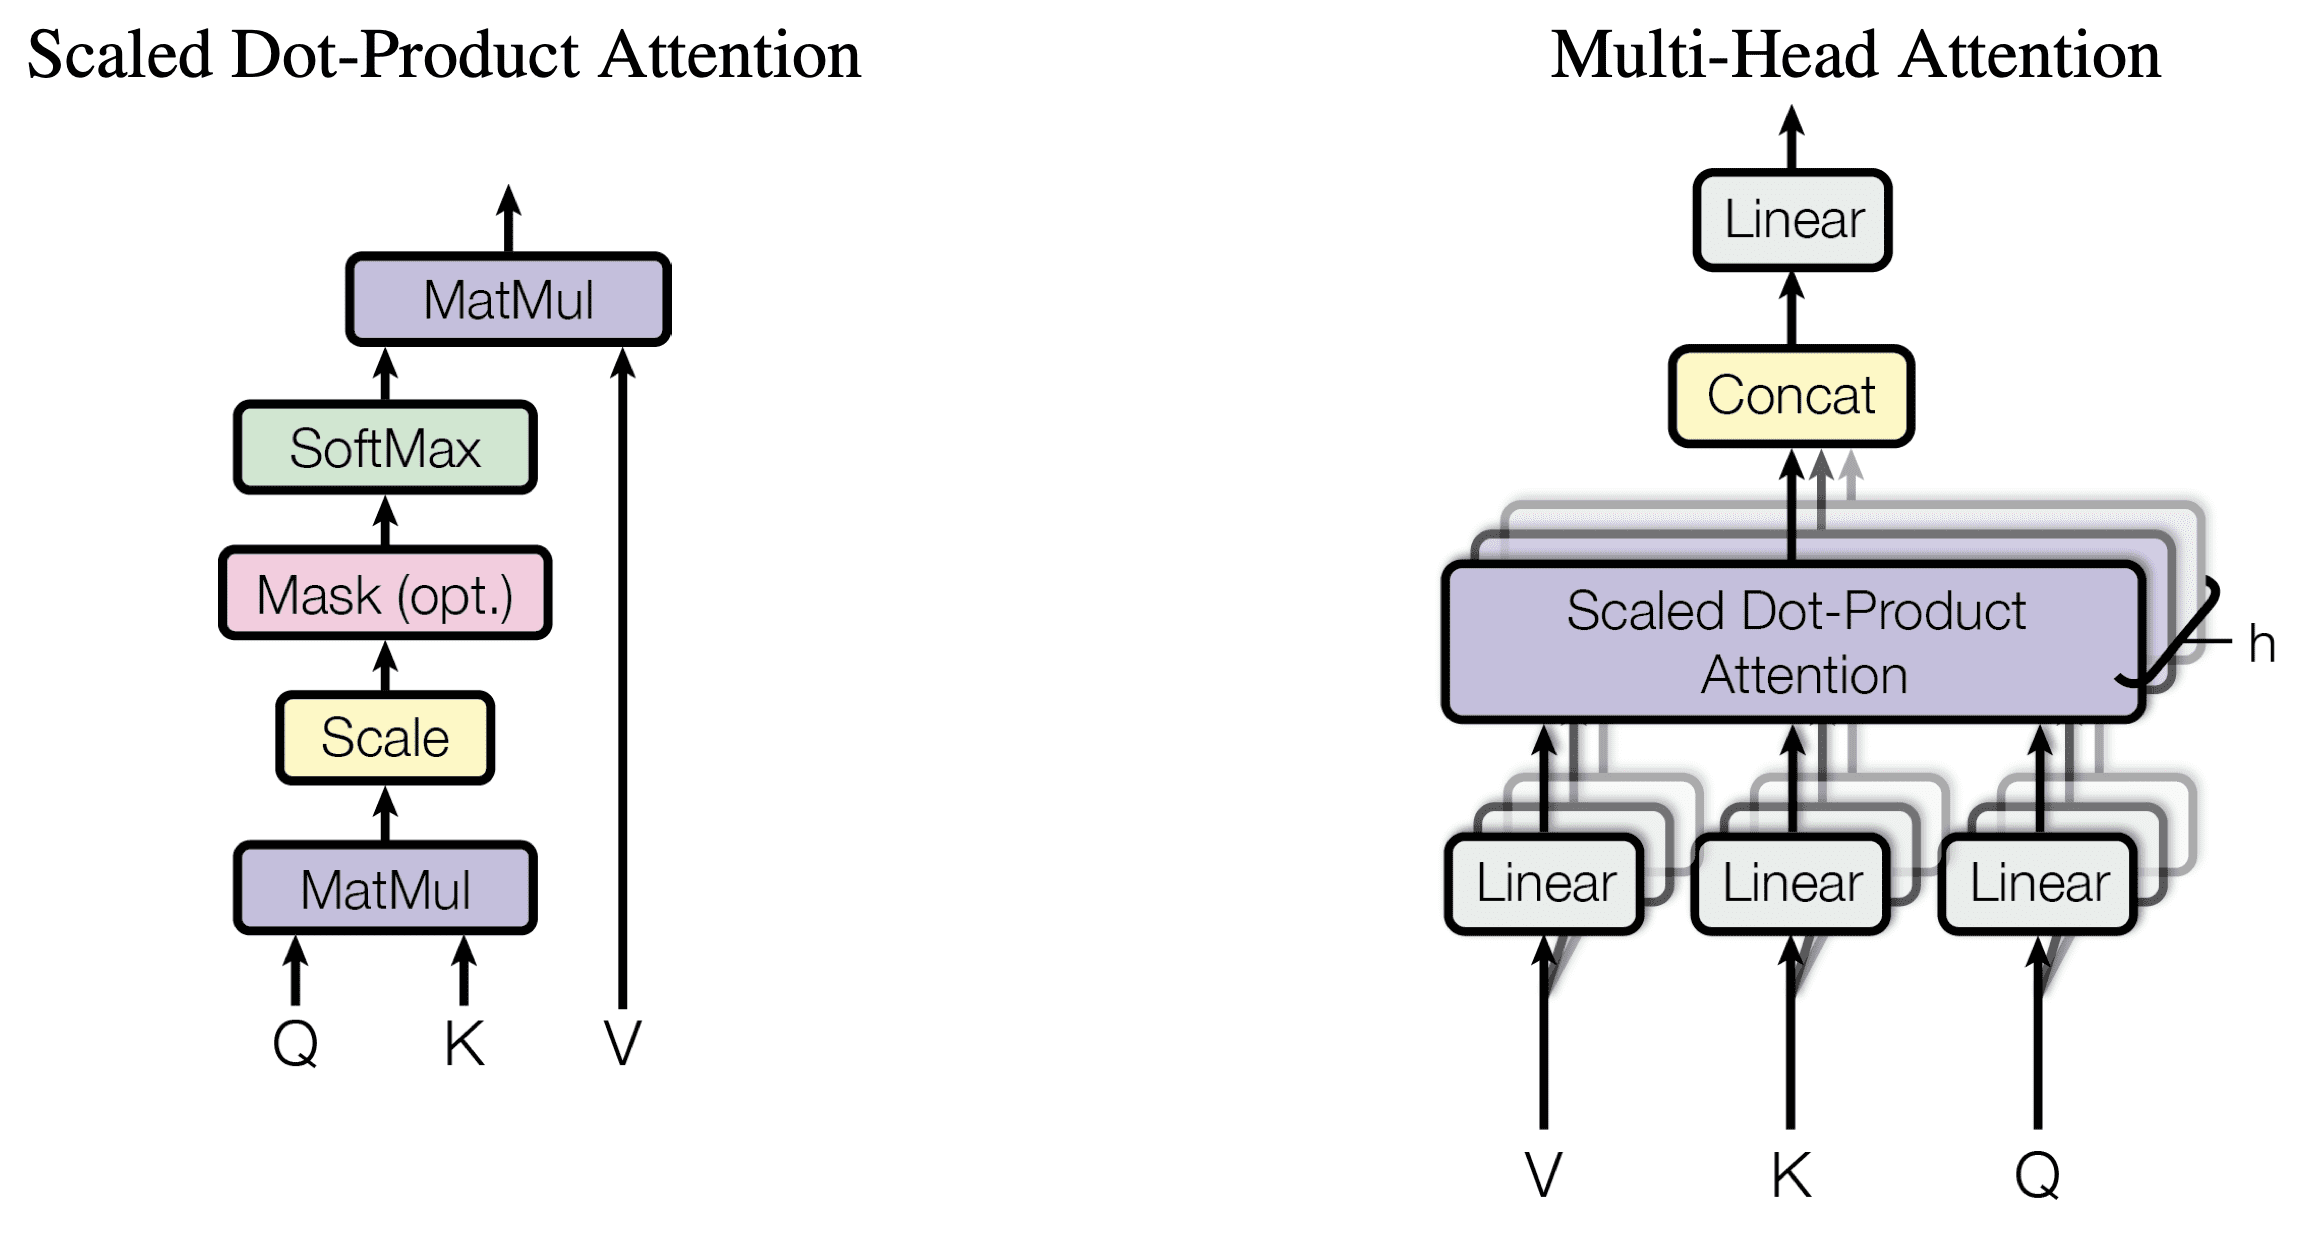
\includegraphics[width=0.6\textwidth]{scaled_dot_product_attention.png}
    \captionof{figure}{Sơ đồ Scaled Dot-Product Attention. Đầu vào là các ma trận Q, K, V và đầu ra là một ma trận đã được làm giàu ngữ cảnh.}
    \label{fig:scaled_dot_product_attention}
\end{center}

\subsubsection{Multi-Head Attention}
\paragraph{Vấn đề của Single-Head Attention}
Chỉ có một bộ Self-Attention duy nhất sẽ bị hạn chế. Nó giống như việc bạn chỉ có thể tập trung vào một khía cạnh của mối quan hệ giữa các từ. Ví dụ, khi xử lý câu "Con mèo ngồi trên chiếu", một "đầu" chú ý (attention head) có thể học cách liên kết "nó" với "mèo" (quan hệ đồng tham chiếu), nhưng có thể sẽ bỏ lỡ các mối quan hệ khác (ví dụ, quan hệ cú pháp).

\paragraph{Giải pháp: Nhiều "đầu" chú ý song song}
Multi-Head Attention giải quyết vấn đề này bằng cách chạy nhiều cơ chế Scaled Dot-Product Attention một cách \textbf{song song}.
\begin{itemize}
    \item Thay vì chỉ có một bộ trọng số $(W^Q, W^K, W^V)$, chúng ta có $h$ bộ (ví dụ, $h=8$).
    \item Mỗi bộ trọng số này $(W^Q_i, W^K_i, W^V_i)$ với $i=1,\dots,h$ được gọi là một "đầu" chú ý.
    \item Mỗi "đầu" sẽ chiếu các vector đầu vào vào một không gian con khác nhau và thực hiện Self-Attention một cách độc lập. Điều này cho phép mỗi đầu có thể học một loại quan hệ khác nhau. Ví dụ, một đầu có thể học quan hệ cú pháp, một đầu khác học quan hệ ngữ nghĩa, một đầu khác học quan hệ đồng tham chiếu...
    \item Các vector đầu ra từ tất cả các đầu sau đó được \textbf{nối lại (concatenated)} với nhau.
    \item Vector nối này sau đó được chiếu qua một ma trận trọng số cuối cùng $W^O$ để tạo ra vector đầu ra cuối cùng của lớp Multi-Head Attention.
\end{itemize}

\begin{center}
    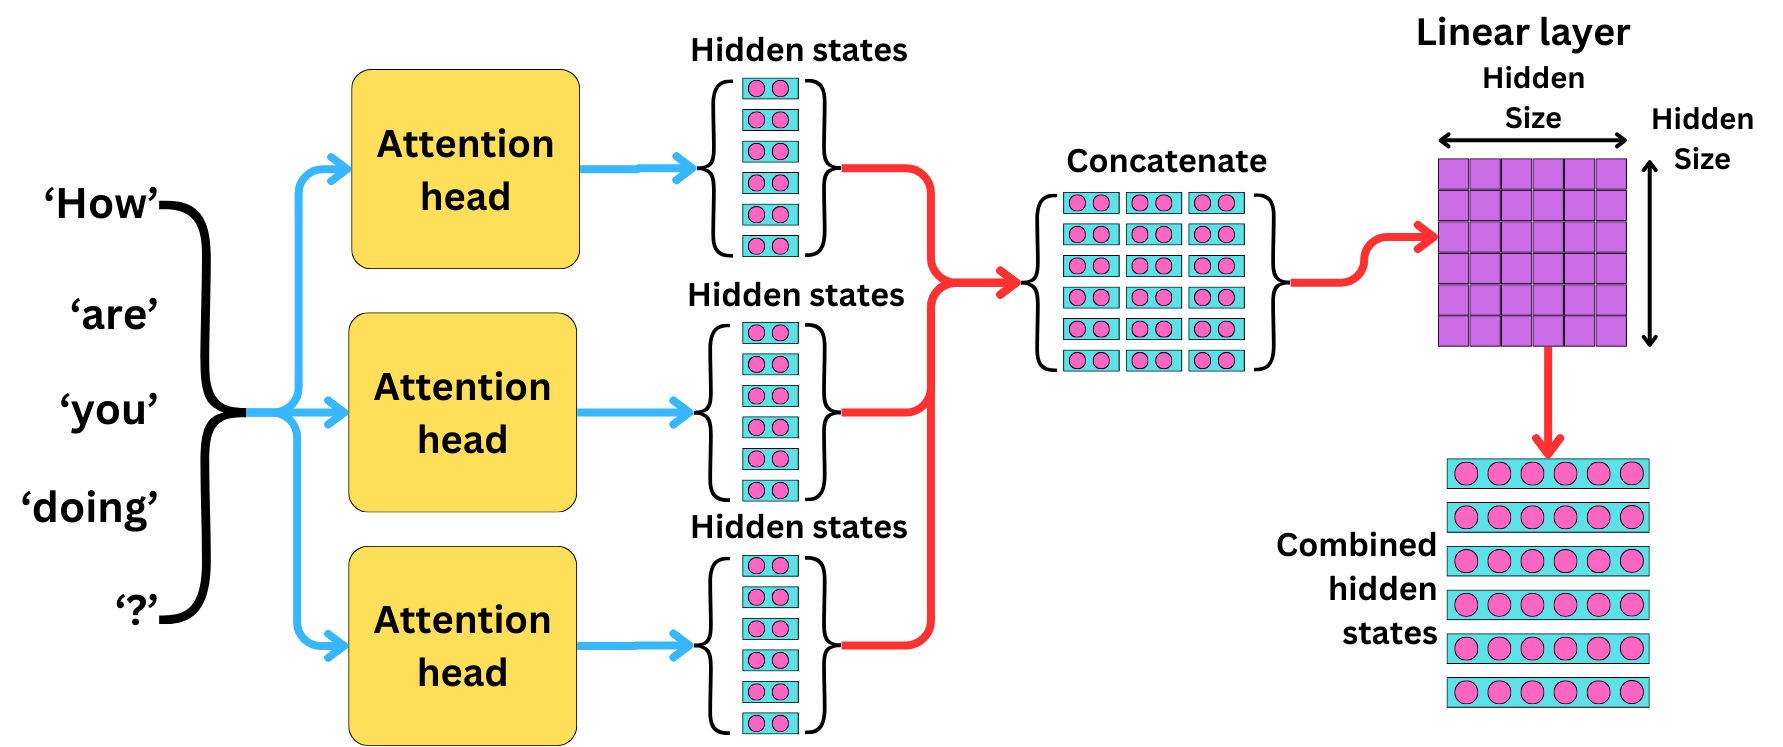
\includegraphics[width=0.8\textwidth]{multi_head_attention.png}
    \captionof{figure}{Kiến trúc Multi-Head Attention, bao gồm nhiều "đầu" Scaled Dot-Product Attention chạy song song.}
    \label{fig:multi_head_attention}
\end{center}

Multi-Head Attention cho phép mô hình cùng lúc chú ý đến thông tin từ các không gian biểu diễn khác nhau tại các vị trí khác nhau. Đây là một trong những nhân tố chính tạo nên sức mạnh biểu diễn của Transformer.

\subsection{Kiến trúc Encoder-Decoder và các thành phần phụ}
\label{ssec:transformer_architecture}
Transformer gốc vẫn giữ kiến trúc Encoder-Decoder của Seq2Seq, nhưng thay thế hoàn toàn các lớp RNN bằng các khối Self-Attention và các lớp Feed-Forward.

\subsubsection{The Encoder Stack}
Encoder của Transformer là một chuỗi gồm $N$ (ví dụ, $N=6$) khối Encoder giống hệt nhau được xếp chồng lên nhau. Mỗi khối bao gồm hai lớp con chính:
\begin{enumerate}
    \item \textbf{Multi-Head Self-Attention Layer:} Lớp này thực hiện Self-Attention trên chuỗi đầu vào.
    \item \textbf{Position-wise Feed-Forward Network (FFN):} Đây là một mạng nơ-ron truyền thẳng đơn giản, bao gồm hai lớp tuyến tính với một hàm kích hoạt ReLU ở giữa.
        $$ \text{FFN}(x) = \max(0, xW_1 + b_1)W_2 + b_2 $$
        FFN này được áp dụng một cách \textbf{độc lập và giống hệt nhau} cho từng vị trí (position) trong chuỗi.
\end{enumerate}
Ngoài ra, mỗi lớp con này còn được bao bọc bởi hai thành phần quan trọng khác:
\begin{itemize}
    \item \textbf{Residual Connection (Kết nối phần dư):} Đầu ra của mỗi lớp con là $\text{LayerNorm}(x + \text{Sublayer}(x))$. Tức là, đầu vào $x$ của lớp con được cộng trực tiếp vào đầu ra của chính lớp đó ($\text{Sublayer}(x)$). Kết nối phần dư này giúp gradient chảy dễ dàng hơn qua các mạng sâu và chống lại vấn đề triệt tiêu gradient.
    \item \textbf{Layer Normalization (Chuẩn hóa lớp):} Chuẩn hóa đầu ra của mỗi lớp con để ổn định quá trình huấn luyện.
\end{itemize}
\begin{tcolorbox}[
    title={Vai trò của các Thành phần Phụ trong Khối Transformer},
    colback=blue!5!white, colframe=blue!50!black, fonttitle=\bfseries
]
Nếu Self-Attention là "bộ não" thì FFN, Residual Connection và Layer Normalization là "hệ tuần hoàn và hệ thần kinh" giúp bộ não đó hoạt động ổn định và hiệu quả.
\begin{itemize}
    \item \textbf{Position-wise Feed-Forward Network (FFN):}
        \begin{itemize}
            \item \textbf{Vai trò:} Lớp Self-Attention chủ yếu thực hiện việc \textbf{trộn thông tin (mixing information)} giữa các từ. Sau bước này, lớp FFN được áp dụng riêng lẻ cho từng vị trí để \textbf{xử lý sâu hơn (deep processing)} thông tin đã được trộn đó. Nó có thể được xem như một bước "biến đổi phi tuyến" mạnh mẽ, giúp mô hình học các mối quan hệ phức tạp hơn, hoặc thậm chí hoạt động như một bộ nhớ key-value đơn giản để lưu trữ các tri thức đã học.
            \item \textbf{Tại sao "Position-wise"?} Việc áp dụng cùng một FFN cho mọi vị trí tương tự như việc chia sẻ trọng số trong RNN hoặc phép tích chập 1x1 trong CNN. Nó đảm bảo tính nhất quán trong cách xử lý ở các vị trí khác nhau.
        \end{itemize}
    \item \textbf{Residual Connection \& Layer Normalization:}
        \begin{itemize}
            \item \textbf{Mục đích kép của Residual Connection:} 1) Nó tạo ra một "con đường tắt" cho gradient, giúp chống lại vấn đề triệt tiêu gradient và cho phép huấn luyện các mô hình rất sâu (ví dụ, hàng chục lớp Transformer). 2) Nó đảm bảo rằng ngay cả khi một lớp con (Sublayer) không học được gì hữu ích, thông tin từ lớp trước đó vẫn có thể đi thẳng tới lớp tiếp theo mà không bị mất mát. Mô hình chỉ cần học phần "thay đổi" (delta) so với đầu vào.
            \item \textbf{Layer Normalization:} Nó giúp ổn định quá trình huấn luyện bằng cách giữ cho đầu ra của mỗi lớp con có phân phối ổn định (trung bình 0, phương sai 1). Điều này làm cho quá trình tối ưu hóa trở nên mượt mà hơn và ít nhạy cảm hơn với việc khởi tạo trọng số. Sự kết hợp của Residuals và Norm là công thức vàng để huấn luyện các mạng nơ-ron rất sâu thành công.
        \end{itemize}
\end{itemize}
\end{tcolorbox}
\subsubsection{The Decoder Stack}
Decoder cũng là một chuỗi gồm $N$ khối Decoder giống hệt nhau. Mỗi khối Decoder có ba lớp con:
\begin{enumerate}
    \item \textbf{Masked Multi-Head Self-Attention Layer:} Tương tự như Self-Attention của Encoder, nhưng có một sự thay đổi quan trọng: \textbf{masking (che giấu)}. Khi dự đoán từ ở vị trí $i$, Decoder chỉ được phép "chú ý" đến các từ ở các vị trí trước đó (từ $1$ đến $i$).
    \begin{itemize}
        \item \textbf{Cơ chế kỹ thuật:} Việc này được thực hiện bằng cách thêm một "ma trận mặt nạ" (mask matrix) vào ma trận điểm chú ý, ngay trước bước softmax. Ma trận này có giá trị là 0 cho các vị trí được phép chú ý và $-\infty$ cho các vị trí bị cấm.
        \item \textbf{Hệ quả:} Sau khi qua hàm softmax, các vị trí có giá trị $-\infty$ sẽ có trọng số chú ý bằng 0, đảm bảo rằng thông tin từ các từ tương lai không bị "rò rỉ" vào quá trình tính toán.
        \item \textbf{Mục đích:} Điều này là để đảm bảo tính \textbf{tự hồi quy (auto-regressive)} của mô hình, ngăn không cho nó "gian lận" bằng cách nhìn vào các từ mà nó đang cố gắng dự đoán. Nó mô phỏng quá trình sinh văn bản trong thực tế, nơi chúng ta chỉ biết những từ đã viết trước đó.
    \end{itemize}
    \item \textbf{Multi-Head Cross-Attention Layer:} Đây là nơi Decoder thực sự tương tác với Encoder, và là nơi kiến trúc "chú ý" của Seq2Seq gốc được tái hiện.
    \begin{itemize}
        \item \textbf{Dòng chảy thông tin:} Ở lớp này, \textbf{Query} được tạo ra từ đầu ra của lớp Masked Self-Attention của Decoder. Nó đại diện cho "câu hỏi" mà Decoder đang muốn hỏi: "Dựa trên những gì tôi đã dịch cho đến nay, tôi nên nhìn vào đâu trong câu gốc để dịch từ tiếp theo?".
        \item Trong khi đó, \textbf{Key và Value} được tạo ra từ \textbf{đầu ra của khối Encoder cuối cùng}. Chúng đại diện cho "kho thông tin" mà Decoder có thể truy vấn.
        \item \textbf{Kết quả:} Lớp này cho phép mỗi từ trong chuỗi đầu ra chú ý đến tất cả các từ trong chuỗi đầu vào, giúp mô hình căn chỉnh (align) các từ giữa hai ngôn ngữ một cách hiệu quả.
    \end{itemize}
    \item \textbf{Position-wise Feed-Forward Network:} Giống hệt như trong Encoder.
\end{enumerate}
Tương tự Encoder, mỗi lớp con của Decoder cũng có Residual Connection và Layer Normalization.

\subsubsection{Huấn luyện và Tối ưu hóa}
\label{sssec:transformer_training}
Kiến trúc Transformer gốc được huấn luyện cho tác vụ dịch máy. Tương tự như mô hình Seq2Seq, mục tiêu là tối thiểu hóa hàm mất mát \textbf{Cross-Entropy} giữa phân phối xác suất đầu ra của Decoder và từ tham chiếu (ground truth).

\begin{itemize}
    \item \textbf{Hàm Mất mát:} Lỗi được tính toán tại mỗi bước sinh từ của Decoder và được tổng hợp lại trên toàn bộ chuỗi.
    \item \textbf{Tối ưu hóa:} Bài báo gốc sử dụng bộ tối ưu hóa \textbf{Adam} \cite{kingma2014adam} với một lịch trình tốc độ học (learning rate schedule) đặc biệt bao gồm một giai đoạn "warmup" (tăng tuyến tính) sau đó là giảm dần theo hàm căn bậc hai nghịch đảo. Lịch trình này được chứng minh là rất quan trọng để huấn luyện Transformer một cách ổn định.
    \item \textbf{Điều chuẩn (Regularization):} Hai kỹ thuật điều chuẩn chính được sử dụng để tránh overfitting là \textbf{Dropout} \cite{srivastava2014dropout}, được áp dụng sau mỗi lớp con (trước kết nối phần dư), và \textbf{Label Smoothing}, một kỹ thuật làm cho các nhãn thật trở nên "mềm" hơn một chút (ví dụ, thay vì [0, 0, 1, 0], nhãn có thể là [0.025, 0.025, 0.9, 0.025]), giúp mô hình bớt tự tin thái quá và tổng quát hóa tốt hơn.
\end{itemize}

\subsection{Positional Encoding: Thêm thông tin về vị trí}
\label{ssec:positional_encoding_intro}

Một vấn đề lớn của việc loại bỏ RNN là chúng ta đã làm mất thông tin về \textbf{thứ tự của các từ}. Self-Attention, về bản chất, không nhạy cảm với vị trí; nếu ta hoán vị các từ trong câu, ma trận chú ý cũng sẽ bị hoán vị tương ứng mà không thay đổi bản chất.

Để giải quyết vấn đề này, Transformer thêm một vector gọi là \textbf{Positional Encoding (Mã hóa Vị trí)} vào các vector embedding đầu vào. Vector này cung cấp thông tin về vị trí tuyệt đối hoặc tương đối của một từ trong chuỗi.

\subsubsection{Absolute Positional Encoding (Sinusoidal)}
Đây là phương pháp được sử dụng trong bài báo gốc. Các vector mã hóa vị trí được tạo ra bằng các hàm sin và cos với các tần số khác nhau:
$$ PE_{(pos, 2i)} = \sin(pos / 10000^{2i/d_{\text{model}}}) $$
$$ PE_{(pos, 2i+1)} = \cos(pos / 10000^{2i/d_{\text{model}}}) $$
Trong đó $pos$ là vị trí của từ, $i$ là chỉ số chiều của vector, và $d_{\text{model}}$ là số chiều của embedding.
\paragraph{Tại sao lại dùng sin và cos?}
\begin{itemize}
    \item \textbf{Giá trị duy nhất:} Mỗi vị trí có một vector mã hóa duy nhất.
    \item \textbf{Mô hình có thể học quan hệ tương đối:} Có một tính chất toán học quan trọng: mã hóa vị trí của $pos+k$ có thể được biểu diễn như một hàm tuyến tính của mã hóa vị trí của $pos$. Điều này cho phép mô hình dễ dàng học cách chú ý đến các vị trí tương đối, ví dụ "từ cách 2 vị trí về bên phải".
    \item \textbf{Khả năng ngoại suy:} Có thể tạo ra vector mã hóa cho các chuỗi dài hơn những chuỗi đã thấy trong quá trình huấn luyện.
\end{itemize}

\subsubsection{Relative Positional Encoding}
Các phương pháp sau này cho rằng thông tin về khoảng cách tương đối ("từ này cách từ kia bao xa?") quan trọng hơn vị trí tuyệt đối. Các phương pháp mã hóa vị trí tương đối sẽ sửa đổi trực tiếp cơ chế Self-Attention, thêm một số hạng biểu diễn cho khoảng cách tương đối vào lúc tính điểm chú ý.

\subsubsection{Rotary Position Embedding (RoPE)}
Đây là một phương pháp mã hóa vị trí tương đối rất thanh lịch và hiệu quả \cite{su2021roformer}, được sử dụng trong nhiều LLM hiện đại như Llama.
\begin{itemize}
    \item \textbf{Ý tưởng:} Thay vì cộng, RoPE \textbf{xoay (rotates)} các vector Query và Key một góc phụ thuộc vào vị trí tuyệt đối của chúng.
    \item \textbf{Hệ quả:} Tích vô hướng giữa hai vector đã được xoay ($q_m^T k_n$) sẽ chỉ phụ thuộc vào vector ban đầu và \textbf{khoảng cách tương đối} giữa chúng ($m-n$), chứ không phụ thuộc vào vị trí tuyệt đối $m, n$.
\end{itemize}
RoPE đã chứng tỏ khả năng ngoại suy độ dài ngữ cảnh rất tốt và là một trong những phương pháp mã hóa vị trí hàng đầu hiện nay.
% % !TEX root = ../main.tex
% File: chapters_part1/chap4_2.tex
% Nội dung cho Chương 4, Phần 2

\section{Phân loại Kiến trúc LLMs}
\label{sec:llm_architectures_classification}

Kiến trúc Transformer gốc mà chúng ta vừa phân tích là một mô hình Encoder-Decoder hoàn chỉnh, được thiết kế cho các tác vụ chuỗi-sang-chuỗi (sequence-to-sequence). Tuy nhiên, các nhà nghiên cứu nhanh chóng nhận ra rằng bằng cách chỉ sử dụng một phần của kiến trúc này -- hoặc chỉ Encoder, hoặc chỉ Decoder -- họ có thể tạo ra các mô hình được chuyên môn hóa cao và cực kỳ hiệu quả cho các loại tác vụ khác nhau.

Sự phân tách này đã khai sinh ra ba "họ" kiến trúc chính, định hình nên toàn bộ bối cảnh của các Mô hình Ngôn ngữ Lớn (LLMs) ngày nay. Hiểu rõ ba họ kiến trúc này là chìa khóa để lựa chọn mô hình phù hợp cho ứng dụng của bạn.

\subsection{Họ Mô hình chỉ Encoder (Encoder-Only): Bậc thầy của Sự Hiểu Ngôn ngữ}
\label{ssec:encoder_only}

Các mô hình thuộc họ này chỉ sử dụng khối Encoder của kiến trúc Transformer. Chúng được thiết kế với một mục tiêu duy nhất: tạo ra các \textbf{biểu diễn ngữ cảnh sâu sắc (deep contextualized representations)} cho văn bản đầu vào.

\begin{tcolorbox}[
    title=Triết lý của Encoder-Only,
    colback=blue!5!white, colframe=blue!75!black, fonttitle=\bfseries
]
"Để thực sự hiểu ý nghĩa của một từ trong câu, tôi cần phải nhìn vào \textbf{cả hai phía}: những từ đứng trước nó và những từ đứng sau nó."
\end{tcolorbox}

\subsubsection{Kiến trúc và Mục tiêu Huấn luyện Nền tảng}
\paragraph{Kiến trúc và Tính hai chiều (Bidirectionality)}
Đây là đặc điểm quan trọng nhất. Nhờ cơ chế Self-Attention không bị che (unmasked), tại mỗi lớp, mỗi từ có thể "chú ý" đến tất cả các từ khác trong câu, cả bên trái và bên phải. Điều này cho phép mô hình xây dựng một sự hiểu biết toàn diện về ngữ cảnh, điều mà các mô hình hồi tiếp (RNN) hay tự hồi quy (Decoder-Only) không thể làm được. Đầu ra của mô hình là một chuỗi các vector embedding, mỗi vector tương ứng với một token đầu vào, nhưng đã được "làm giàu" bởi thông tin ngữ cảnh hai chiều sâu sắc.

\paragraph{Mục tiêu Huấn luyện: Masked Language Modeling (MLM)}
MLM là mục tiêu huấn luyện cốt lõi của BERT và nhiều mô hình kế nhiệm.
\begin{itemize}
    \item \textbf{Cơ chế:} Lấy một câu đầu vào, che (mask) ngẫu nhiên khoảng 15\% số token bằng một token đặc biệt `[MASK]`. Sau đó, nhiệm vụ của mô hình là \textbf{dự đoán các token gốc đã bị che}, dựa vào các token không bị che xung quanh.
    \item \textbf{Tại sao lại hiệu quả?} MLM buộc mô hình phải học các mối quan hệ ngữ nghĩa và cú pháp sâu sắc từ cả hai phía để có thể "điền vào chỗ trống". Nó không chỉ là dự đoán từ tiếp theo, mà là một bài kiểm tra "đọc hiểu" thực sự.
\end{itemize}

\begin{center}
    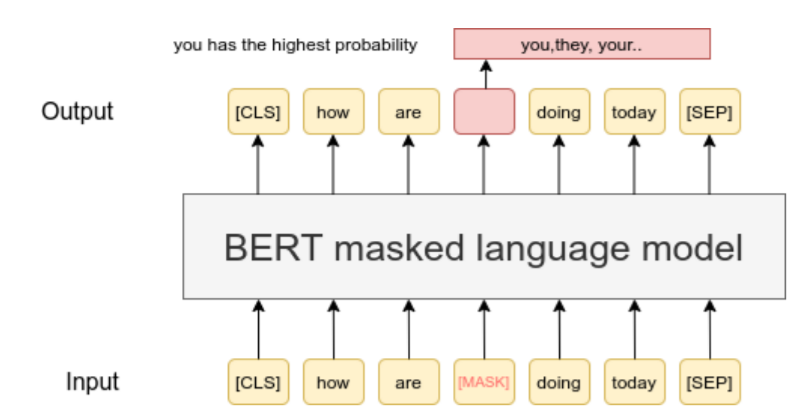
\includegraphics[width=0.8\textwidth]{bert_mlm_nsp.png}
    \captionof{figure}{Mục tiêu huấn luyện kinh điển của BERT: Masked Language Modeling (MLM). Mô hình phải dự đoán các token bị che dựa trên ngữ cảnh hai chiều.}
    \label{fig:bert_mlm_nsp}
\end{center}

\subsubsection{Sự phát triển và các biến thể của Họ Encoder-Only}
Từ nền tảng của BERT, một hệ sinh thái đa dạng các mô hình Encoder-Only đã ra đời, mỗi loại được tối ưu cho các mục đích khác nhau: hiệu suất, kích thước, tác vụ cụ thể, hay miền kiến thức chuyên biệt.

\paragraph{1. Gia đình BERT: Những người kế nhiệm trực tiếp}
Đây là các mô hình cải tiến trực tiếp từ kiến trúc và phương pháp huấn luyện của BERT.
\begin{itemize}
    \item \textbf{RoBERTa (Facebook) \cite{liu2019roberta}:} Không thay đổi kiến trúc, nhưng chứng minh rằng việc tối ưu hóa kỹ lưỡng quá trình huấn luyện có thể mang lại hiệu quả vượt trội. Các cải tiến chính bao gồm: huấn luyện lâu hơn, trên nhiều dữ liệu hơn, với batch size lớn hơn, loại bỏ mục tiêu NSP (Next Sentence Prediction), và sử dụng "che động" (dynamic masking).
    \item \textbf{DistilBERT (Hugging Face) \cite{sanh2019distilbert}:} Một phiên bản "chưng cất" nhỏ hơn, nhanh hơn của BERT. Nó sử dụng kỹ thuật \textit{knowledge distillation}, trong đó một mô hình "học trò" (student) nhỏ hơn học cách bắt chước đầu ra của một mô hình "giáo viên" (teacher) lớn hơn (BERT). DistilBERT giữ lại 97\% hiệu năng của BERT nhưng chỉ có 60\% kích thước.
    \item \textbf{ALBERT (Google) \cite{lan2019albert}:} Một cách tiếp cận khác để giảm tham số. ALBERT sử dụng hai kỹ thuật chính: \textit{factorized embedding parameterization} (phân tách ma trận embedding từ lớn thành hai ma trận nhỏ) và \textit{cross-layer parameter sharing} (chia sẻ trọng số của các khối Transformer với nhau).
    \item \textbf{SpanBERT (Facebook) \cite{joshi2020spanbert}:} Tối ưu hóa BERT cho các tác vụ cần hiểu các \textbf{đoạn văn bản (spans)} liên tục, như Hỏi-đáp trích xuất. Thay vì che các token ngẫu nhiên, SpanBERT che các đoạn ngẫu nhiên và huấn luyện mô hình dự đoán toàn bộ đoạn bị che chỉ từ các token ở biên của đoạn đó.
\end{itemize}

\paragraph{2. Các mô hình Biểu diễn Câu: Chuyên gia về Tìm kiếm Ngữ nghĩa}
Một hạn chế của BERT gốc là nó không tạo ra các vector biểu diễn câu (sentence embeddings) tốt "ngay lập tức". Việc lấy embedding của token `[CLS]` hoặc lấy trung bình các token embedding thường cho kết quả tìm kiếm tương đồng không cao. Nhánh mô hình này giải quyết vấn đề đó.
\begin{itemize}
    \item \textbf{SBERT (Sentence-BERT) \cite{reimers2019sentence}:} Là mô hình tiên phong. SBERT tinh chỉnh BERT trên các cặp câu bằng cách sử dụng kiến trúc \textit{siamese} hoặc \textit{triplet}. Kiến trúc này buộc mô hình phải tạo ra một không gian vector mà ở đó các câu có ngữ nghĩa giống nhau sẽ có vector gần nhau (cosine similarity cao) và ngược lại.
    \item \textbf{SimCSE (Simple Contrastive Sentence Embedding) \cite{gao2021simcse}:} Một phương pháp học tương phản (contrastive learning) đơn giản nhưng cực kỳ hiệu quả. Để tạo một cặp dương, SimCSE chỉ cần đưa cùng một câu qua mô hình BERT hai lần (với dropout khác nhau). Các câu khác trong batch được coi là cặp âm. Kỹ thuật này tạo ra các embedding câu chất lượng rất cao mà không cần dữ liệu gán nhãn.
    \item \textbf{E5 (Embeddings from bidErectional Encoder rEpresentations \cite{wang2022text}), Contriever, etc.:} Là thế hệ mô hình embedding mới nhất, được huấn luyện đặc biệt cho các tác vụ \textbf{tìm kiếm (retrieval)}, đặc biệt là tìm kiếm bất đối xứng (truy vấn ngắn, tài liệu dài). Chúng thường đạt hiệu năng SOTA trên các benchmark tìm kiếm ngữ nghĩa.
\end{itemize}

\paragraph{3. Các mô hình cho Miền chuyên biệt và Đa ngôn ngữ}
Ý tưởng cốt lõi là một mô hình được huấn luyện trước trên dữ liệu chuyên ngành sẽ hiểu thuật ngữ và ngữ cảnh của ngành đó tốt hơn.
\begin{itemize}
    \item \textbf{SciBERT \cite{beltagy2019scibert}, BioBERT \cite{lee2020biobert}, ClinicalBERT \cite{alsentzer2019publicly}:} Được huấn luyện trên các kho văn bản khoa học, y sinh, và y tế lâm sàng.
    \item \textbf{FinBERT:} Chuyên cho lĩnh vực tài chính.
    \item \textbf{LegalBERT:} Chuyên cho lĩnh vực pháp luật.
    \item \textbf{CamemBERT \cite{martin2019camembert} (Pháp), PhoBERT \cite{nguyen2020phobert} (Việt), etc.:} Là các mô hình theo kiến trúc RoBERTa nhưng được huấn luyện từ đầu trên kho dữ liệu lớn của một ngôn ngữ cụ thể, cho hiệu năng vượt trội so với các mô hình đa ngôn ngữ trên ngôn ngữ đó.
\end{itemize}

\paragraph{4. Các Encoder Hiện đại, Gọn nhẹ và Hiệu quả}
Nhánh này tập trung vào việc tạo ra các mô hình nhỏ gọn hơn nhưng vẫn giữ được hiệu năng cao thông qua các cải tiến về kiến trúc và mục tiêu huấn luyện.
\begin{itemize}
    \item \textbf{MiniLM (Microsoft) \cite{wang2020minilm}:} Sử dụng một phương pháp chưng cất tri thức sâu, trong đó mô hình học trò không chỉ bắt chước đầu ra cuối cùng mà còn cả ma trận chú ý và mối quan hệ giữa các vector value từ mô hình giáo viên.
    \item \textbf{DeBERTa (Microsoft) \cite{he2020deberta}:} Một trong những encoder mạnh nhất hiện nay. DeBERTa giới thiệu cơ chế \textit{disentangled attention}, tách rời việc mã hóa nội dung từ và vị trí tương đối của chúng.
    \item \textbf{MPNet (Microsoft) \cite{song2020mpnet}:} Kết hợp τα tốt nhất của cả hai thế giới: MLM (BERT) và Permuted Language Modeling (XLNet). Nó giải quyết sự không tương thích giữa pre-training và fine-tuning, cho phép mô hình học các phụ thuộc hai chiều một cách toàn diện hơn.
\end{itemize}

\paragraph{5. Các Encoder với Mục tiêu Huấn luyện khác MLM}
MLM không phải là cách duy nhất để huấn luyện một encoder hai chiều.
\begin{itemize}
    \item \textbf{ELECTRA (Google) \cite{clark2020electra}:} Sử dụng một tác vụ hiệu quả hơn là \textit{replaced token detection}. Một mô hình "generator" nhỏ sẽ thay thế một số token trong câu, và mô hình "discriminator" (chính là ELECTRA) phải dự đoán xem mỗi token là gốc hay đã bị thay thế. Tác vụ này hiệu quả hơn vì mô hình học từ \textit{tất cả} các token, không chỉ 15% bị che.
    \item \textbf{XLNet (Google/CMU) \cite{yang2019xlnet}:} Một mô hình \textit{tự hồi quy hoán vị (permutation-based autoregressive)}. Nó dự đoán các token trong câu theo một thứ tự ngẫu nhiên. Bằng cách này, nó có thể "nhìn thấy" ngữ cảnh từ cả hai phía (giống BERT) trong khi vẫn giữ được các lợi ích của mô hình tự hồi quy.
\end{itemize}

\begin{tcolorbox}[
    title=Tổng kết: Điểm mạnh và Ứng dụng của Encoder-Only,
    colback=blue!5!white, colframe=blue!75!black, fonttitle=\bfseries
]
\textbf{Nguyên tắc chung:} Sử dụng mô hình Encoder-Only khi tác vụ của bạn đòi hỏi sự \textbf{hiểu sâu sắc về toàn bộ văn bản đầu vào} và đầu ra không phải là một chuỗi văn bản mới, mạch lạc. Chúng là các mô hình \textbf{NLU (Natural Language Understanding)} chứ không phải \textbf{NLG (Natural Language Generation)}.

\textbf{Ứng dụng điển hình:}
\begin{itemize}
    \item \textbf{Phân loại văn bản (Text Classification):} Phân tích cảm xúc, phát hiện chủ đề, kiểm duyệt nội dung (toxic detection). Mô hình cần hiểu toàn bộ câu để đưa ra một nhãn duy nhất.
    \item \textbf{Gán nhãn chuỗi (Token Classification):} Nhận dạng Thực thể Tên (NER), Gán nhãn Từ loại (POS Tagging). Mô hình cần hiểu ngữ cảnh xung quanh mỗi từ để gán nhãn cho nó.
    \item \textbf{Tìm kiếm Ngữ nghĩa (Semantic Search):} Biến các câu/tài liệu thành các vector embedding có ý nghĩa (sử dụng các mô hình như SBERT, E5). Các vector này sau đó được lưu trữ và truy vấn bằng các thuật toán tìm kiếm lân cận gần nhất (ANN).
    \item \textbf{Hỏi-đáp trích xuất (Extractive QA):} Tìm và trích xuất một đoạn văn bản (span) làm câu trả lời từ một văn bản ngữ cảnh cho trước.
    \item \textbf{Retrieval-Augmented Generation (RAG):} Đây là một ứng dụng lai. Giai đoạn \textbf{Retrieval (Truy xuất)} trong RAG sử dụng một mô hình Encoder-Only (như E5) để biến truy vấn của người dùng và các tài liệu trong cơ sở tri thức thành vector, sau đó tìm ra các tài liệu liên quan nhất. Các tài liệu này sau đó mới được đưa cho một mô hình sinh (Decoder-Only) để tạo ra câu trả lời.
\end{itemize}
\end{tcolorbox}

\subsection{Họ Mô hình chỉ Decoder (Decoder-Only): Bậc thầy của Sự Sáng tạo}
\label{ssec:decoder_only}
Đây là họ kiến trúc đang thống trị thế giới AI hiện nay, là nền tảng của các mô hình như ChatGPT, Llama, và Claude. Chúng chỉ sử dụng khối Decoder của kiến trúc Transformer.

\begin{tcolorbox}[
    title=Triết lý của Decoder-Only,
    colback=red!5!white, colframe=red!75!black, fonttitle=\bfseries
]
"Để viết tiếp một câu chuyện, tôi chỉ cần biết những gì đã được viết \textbf{trước đó}. Tôi không được phép nhìn vào tương lai."
\end{tcolorbox}

\subsubsection{Kiến trúc và Mục tiêu Huấn luyện Nền tảng}
\paragraph{Kiến trúc Tự hồi quy (Auto-regressive Architecture)}
\begin{itemize}
    \item \textbf{Cấu tạo:} Một chuỗi các khối Decoder của Transformer xếp chồng lên nhau. Quan trọng là, chúng \textbf{không có Encoder} và do đó cũng \textbf{không có lớp Cross-Attention}.
    \item \textbf{Tính một chiều (Unidirectionality):} Đây là đặc điểm nhận dạng. Chúng sử dụng \textbf{Masked Self-Attention}. Tại mỗi vị trí, một từ chỉ có thể "chú ý" đến chính nó và các từ đứng trước nó. Nó không thể nhìn thấy các từ ở phía sau, đảm bảo rằng việc dự đoán chỉ dựa trên thông tin quá khứ.
    \item \textbf{Dòng chảy:} Mô hình nhận vào một chuỗi các từ (prompt) và nhiệm vụ của nó là dự đoán từ \textbf{tiếp theo có khả năng nhất}. Từ được dự đoán sau đó được nối vào chuỗi đầu vào, và quá trình này lặp lại để sinh ra từ tiếp theo, cứ thế tiếp tục.
\end{itemize}

\paragraph{Mục tiêu Huấn luyện: Causal Language Modeling (CLM)}
Đây là mục tiêu huấn luyện duy nhất và rất đơn giản: \textbf{Dự đoán từ tiếp theo (Next Token Prediction)}.
\begin{itemize}
    \item \textbf{Cơ chế:} Mô hình được cho xem một đoạn văn bản và được huấn luyện để, tại mỗi vị trí, dự đoán từ tiếp theo dựa trên tất cả các từ đã có trước đó.
    \item \textbf{Sức mạnh của Quy mô:} Bằng cách cố gắng dự đoán từ tiếp theo trên một kho văn bản khổng lồ (hàng nghìn tỷ từ), mô hình buộc phải học một lượng kiến thức khổng lồ về thế giới, về ngữ pháp, ngữ nghĩa, và các mẫu hình lý luận để có thể đưa ra dự đoán tốt. Đây là nền tảng cho các "khả năng nổi trội" (emergent abilities) của LLMs.
\end{itemize}

\begin{center}
    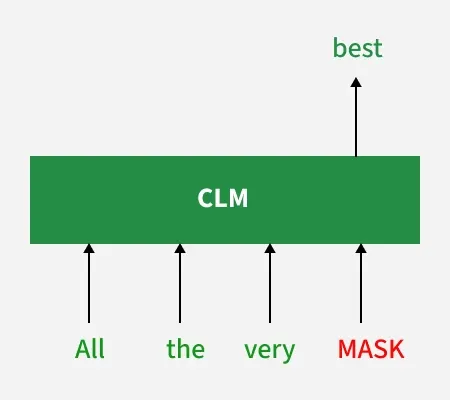
\includegraphics[width=0.8\textwidth]{gpt_clm.png}
    \captionof{figure}{Mục tiêu huấn luyện của GPT: Causal Language Modeling. Tại mỗi bước, mô hình cố gắng dự đoán từ tiếp theo dựa trên các từ trước đó.}
    \label{fig:gpt_clm}
\end{center}

\subsubsection{Sự phát triển và các mô hình tiêu biểu}
Họ mô hình này đã chứng kiến sự phát triển bùng nổ, từ các mô hình tiên phong đến một hệ sinh thái đa dạng các LLMs mã nguồn mở và đóng.

\paragraph{1. Gia đình GPT (OpenAI): Những người tiên phong và dẫn đầu}
Họ mô hình GPT của OpenAI không chỉ định hình nên kiến trúc Decoder-Only mà còn liên tục đẩy lùi các giới hạn của AI.
\begin{itemize}
    \item \textbf{GPT (2018) \cite{radford2018improving}:} Bài báo gốc chứng minh rằng một mô hình Transformer chỉ-Decoder được huấn luyện trước có thể được tinh chỉnh hiệu quả cho các tác vụ NLU.
    \item \textbf{GPT-2 (2019) \cite{radford2019language}:} Gây tiếng vang lớn khi cho thấy việc tăng quy mô (lên tới 1.5 tỷ tham số) có thể tạo ra một mô hình có khả năng sinh văn bản mạch lạc đáng kinh ngạc mà không cần tinh chỉnh (zero-shot).
    \item \textbf{GPT-3 (2020) \cite{brown2020language}:} Mở ra kỷ nguyên LLM thực sự với 175 tỷ tham số. GPT-3 lần đầu tiên thể hiện rõ các \textbf{khả năng nổi trội (emergent abilities)}, đặc biệt là \textbf{học trong ngữ cảnh (in-context learning)}, cho phép nó thực hiện các tác vụ chỉ bằng cách cung cấp vài ví dụ trong prompt (few-shot).
    \item \textbf{InstructGPT \& ChatGPT \cite{ouyang2022training}:} Đánh dấu một bước ngoặt từ "mô hình ngôn ngữ" sang "trợ lý AI" bằng cách sử dụng các kỹ thuật căn chỉnh (alignment) như \textbf{Instruction Tuning} và \textbf{RLHF} (Reinforcement Learning from Human Feedback) để làm cho mô hình hữu ích, trung thực và an toàn hơn.
    \item \textbf{GPT-4 \& GPT-4o (2023-2024) \cite{openai2023gpt4, openai2024gpt4o}:} Là các mô hình SOTA hiện tại, không chỉ mạnh mẽ hơn về ngôn ngữ mà còn trở thành các mô hình \textbf{đa phương thức (multimodal)}, có khả năng hiểu và xử lý cả văn bản, hình ảnh, và âm thanh.
\end{itemize}

\paragraph{2. Làn sóng LLMs Mã nguồn mở và các đối thủ cạnh tranh}
Sự thành công của GPT đã thúc đẩy một làn sóng nghiên cứu và phát triển LLMs trên toàn thế giới, với nhiều mô hình mã nguồn mở mạnh mẽ.
\begin{itemize}
    \item \textbf{LLaMA (Meta) \cite{touvron2023llama}:} Họ mô hình LLaMA (và các phiên bản kế nhiệm LLaMA 2, LLaMA 3) đã "dân chủ hóa" LLMs, cung cấp các mô hình mã nguồn mở có hiệu năng cực kỳ cạnh tranh, tạo điều kiện cho một hệ sinh thái ứng dụng và nghiên cứu khổng lồ.
    \item \textbf{Mistral (Pháp):} Nổi lên như một đối thủ đáng gờm với các mô hình hiệu năng cao nhưng kích thước nhỏ gọn (ví dụ: Mistral 7B \cite{jiang2023mistral}). Họ cũng đi tiên phong trong việc thương mại hóa kiến trúc \textbf{Mixture of Experts (MoE)} với mô hình Mixtral, giúp tăng đáng kể số lượng tham số mà không tăng chi phí suy luận tương ứng.
    \item \textbf{Claude (Anthropic):} Được biết đến với "cửa sổ ngữ cảnh" (context window) rất lớn và tập trung mạnh vào sự an toàn thông qua phương pháp \textbf{Constitutional AI} \cite{bai2022constitutional}.
    \item \textbf{Các mô hình đáng chú ý khác:}
        \begin{itemize}
            \item \textbf{Google:} Gemma (mã nguồn mở), Gemini (mô hình SOTA cạnh tranh với GPT-4).
            \item \textbf{Cohere:} Command R(+), tập trung vào các ứng dụng doanh nghiệp và Retrieval-Augmented Generation (RAG).
            \item \textbf{Các mô hình từ Trung Quốc:} Qwen (Alibaba), Yi, Baichuan, InternLM, DeepSeek, thể hiện sự tiến bộ nhanh chóng của cộng đồng AI Trung Quốc.
            \item \textbf{TII (UAE):} Falcon.
        \end{itemize}
\end{itemize}

\paragraph{3. Các mô hình Decoder-Only chuyên biệt}
Bên cạnh các LLM đa dụng, nhiều mô hình được huấn luyện đặc biệt cho các miền cụ thể.
\begin{itemize}
    \item \textbf{Code LLMs:} Các mô hình được huấn luyện chủ yếu trên dữ liệu mã nguồn để hỗ trợ lập trình. Ví dụ: Codex \cite{chen2021evaluating} (nền tảng của GitHub Copilot đời đầu), StarCoder\cite{li2023starcoder}, CodeLLaMA \cite{roziere2023code}, Phi-3 (Microsoft).
    \item \textbf{Dialogue-focused Models:} Các mô hình được tinh chỉnh đặc biệt cho các tác vụ hội thoại, là tiền thân của các chatbot hiện đại. Ví dụ: DialoGPT (Microsoft) \cite{zhang2019dialogpt}, ChatGLM (Trung Quốc).
\end{itemize}

\begin{tcolorbox}[
    title=Tổng kết: Điểm mạnh và Ứng dụng của Decoder-Only,
    colback=red!5!white, colframe=red!75!black, fonttitle=\bfseries
]
\textbf{Nguyên tắc chung:} Sử dụng mô hình Decoder-Only khi tác vụ của bạn đòi hỏi việc \textbf{sinh ra một chuỗi văn bản mới, mạch lạc, và có tính sáng tạo} dựa trên một ngữ cảnh đầu vào. Chúng là các mô hình \textbf{NLG (Natural Language Generation)} và là nền tảng của AI tạo sinh (Generative AI).

\textbf{Điểm mạnh:}
\begin{itemize}
    \item \textbf{Khả năng sinh văn bản xuất sắc:} Là kiến trúc tốt nhất cho mọi tác vụ NLG.
    \item \textbf{Tính linh hoạt (Zero-shot/Few-shot):} Các mô hình lớn có thể thực hiện nhiều tác vụ chỉ thông qua prompt mà không cần fine-tuning, rất linh hoạt và tiết kiệm chi phí gán nhãn.
\end{itemize}
\textbf{Điểm yếu:}
\begin{itemize}
    \item \textbf{Hiểu ngữ cảnh không sâu bằng Encoder-Only:} Do bản chất một chiều, biểu diễn của một từ không được "nhìn thấy" các từ phía sau. Điều này làm chúng kém tối ưu hơn cho các tác vụ NLU thuần túy so với BERT/RoBERTa.
    \item \textbf{Dễ "ảo giác" (Hallucination):} Có xu hướng bịa đặt thông tin một cách tự tin.
    \item \textbf{Quá trình sinh tuần tự là chậm.}
\end{itemize}

\textbf{Ứng dụng điển hình:}
\begin{itemize}
    \item \textbf{Hệ thống Đối thoại và Trợ lý ảo (Chatbots):} ChatGPT, Claude, Gemini.
    \item \textbf{Sáng tạo nội dung:} Viết văn, làm thơ, soạn email, tóm tắt văn bản (abstractive summarization).
    \item \textbf{Lập trình và Sinh mã (Code Generation):} GitHub Copilot.
    \item \textbf{Giải quyết vấn đề thông qua Prompting:} Bất kỳ tác vụ nào có thể được định dạng dưới dạng "đầu vào -> đầu ra văn bản", từ dịch máy, trả lời câu hỏi, đến lý luận toán học.
\end{itemize}
\end{tcolorbox}


\subsection{Họ Mô hình Encoder-Decoder: Sự kết hợp của hai thế giới}
\label{ssec:encoder_decoder_models}
Họ mô hình này quay trở lại với kiến trúc Transformer gốc ("Attention is All You Need"), sử dụng cả hai thành phần Encoder và Decoder. Mặc dù không còn là tâm điểm chú ý như các LLM Decoder-Only, chúng vẫn là kiến trúc mạnh mẽ và phù hợp nhất cho nhiều tác vụ chuỗi-sang-chuỗi quan trọng.

\begin{tcolorbox}[
    title=Triết lý của Encoder-Decoder,
    colback=green!5!white, colframe=green!60!black, fonttitle=\bfseries
]
"Tôi sẽ dùng một bộ mã hóa hai chiều mạnh mẽ để \textbf{hiểu trọn vẹn} văn bản nguồn, và sau đó dùng một bộ giải mã tự hồi quy để \textbf{sinh ra} văn bản đích dựa trên sự hiểu biết đó."
\end{tcolorbox}

\subsubsection{Kiến trúc và Lợi thế Cốt lõi}
\begin{itemize}
    \item \textbf{Kiến trúc:} Một Encoder hai chiều (giống BERT) để đọc và hiểu toàn bộ chuỗi đầu vào. Một Decoder một chiều (giống GPT) để sinh ra chuỗi đầu ra. Hai thành phần này được kết nối với nhau thông qua cơ chế \textbf{Cross-Attention}, cho phép Decoder "tham khảo" bất kỳ phần nào của chuỗi đầu vào đã được mã hóa ở mỗi bước sinh từ.
    \item \textbf{Lợi thế Cốt lõi:} Sự phân tách vai trò này là một lợi thế không thể thay thế trong các tác vụ đòi hỏi sự hiểu biết sâu sắc về toàn bộ ngữ cảnh nguồn trước khi tạo ra đầu ra. Encoder có thể xây dựng một biểu diễn hai chiều hoàn chỉnh, nắm bắt các mối quan hệ phức tạp trong văn bản nguồn. Decoder sau đó có thể tận dụng biểu diễn phong phú này để tạo ra một đầu ra chính xác và phù hợp hơn.
\end{itemize}

\subsubsection{Sự phát triển và các mô hình tiêu biểu}
Họ Encoder-Decoder có một lịch sử phát triển phong phú, từ mô hình nền tảng đến các biến thể được tối ưu hóa cao cho các tác vụ chuyên biệt.

\paragraph{1. Các mô hình Nền tảng và Đa ngôn ngữ}
\begin{itemize}
    \item \textbf{Transformer (Google, 2017) \cite{vaswani2017attention}:} Bài báo "Attention Is All You Need" chính là khởi nguồn của tất cả. Nó giới thiệu kiến trúc Encoder-Decoder với Self-Attention và đã thay thế hoàn toàn RNN trong các tác vụ dịch máy SOTA thời bấy giờ.
    \item \textbf{T5 (Google, 2019) \cite{raffel2020exploring}:} Phổ biến hóa khung làm việc "Text-to-Text", đối xử mọi bài toán NLP như một tác vụ Seq2Seq, giúp đơn giản hóa và thống nhất quá trình nghiên cứu và ứng dụng.
    \item \textbf{BART (Facebook, 2019) \cite{lewis2019bart}:} Kết hợp các ý tưởng từ BERT (encoder hai chiều) và GPT (decoder tự hồi quy) với mục tiêu huấn luyện khử nhiễu linh hoạt, đặc biệt mạnh mẽ cho các tác vụ sinh văn bản có điều kiện.
    \item \textbf{Các phiên bản Đa ngôn ngữ:} Thành công của các mô hình trên đã dẫn đến các phiên bản đa ngôn ngữ được huấn luyện trên hàng trăm thứ tiếng, bao gồm \textbf{mT5}, \textbf{mBART}, và \textbf{MarianMT} (một mô hình từ Microsoft/Facebook được tối ưu hóa cao cho dịch máy). Gần đây nhất, \textbf{NLLB (No Language Left Behind) \cite{costa2022no}} của Meta đã đẩy giới hạn này đi xa hơn, tập trung vào các ngôn ngữ ít tài nguyên.
\end{itemize}

\paragraph{2. Các biến thể với Mục tiêu Huấn luyện và Kiến trúc Sáng tạo}
Nhiều mô hình đã cải tiến kiến trúc hoặc mục tiêu huấn luyện để đạt hiệu năng vượt trội trên các tác vụ cụ thể, đặc biệt là tóm tắt văn bản.
\begin{itemize}
    \item \textbf{PEGASUS (Google, 2020) \cite{zhang2020pegasus}:} Một mô hình cực kỳ mạnh mẽ cho tóm tắt văn bản. Thay vì che các token (MLM) hay các đoạn (T5), PEGASUS có mục tiêu huấn luyện trước là \textbf{"Gap-Sentences Generation"}. Nó che đi toàn bộ các câu quan trọng trong một tài liệu và yêu cầu mô hình sinh lại các câu đó từ phần còn lại. Điều này mô phỏng rất gần với tác vụ tóm tắt.
    \item \textbf{ProphetNet (Microsoft, 2020) \cite{qi2020prophetnet}:} Cải tiến kiến trúc Decoder để có thể dự đoán \textbf{nhiều bước trong tương lai (future n-gram prediction)} thay vì chỉ một từ tiếp theo. Việc "nhìn xa" này giúp mô hình tránh bị lặp lại và tạo ra các bản tóm tắt chất lượng cao hơn.
    \item \textbf{BERT2BERT \cite{rothe2020leveraging}:} Một kiến trúc đơn giản nhưng hiệu quả, khởi tạo cả Encoder và Decoder bằng các trọng số của một mô hình BERT đã được huấn luyện trước. Đây là một cách "khởi động nóng" (warm-start) hiệu quả cho các tác vụ Seq2Seq như tóm tắt.
    \item \textbf{ByT5 (Google) \cite{xue2022byt5}:} Một biến thể của T5 xử lý trực tiếp \textbf{chuỗi các byte UTF-8} thay vì các token. Cách tiếp cận này loại bỏ sự phức tạp và các lỗi tiềm ẩn của quá trình tokenization, giúp mô hình trở nên mạnh mẽ hơn với nhiễu và đa ngôn ngữ.
\end{itemize}

\paragraph{3. Hướng tới sự Hợp nhất và Linh hoạt}
Các nghiên cứu gần đây tìm cách tạo ra các mô hình linh hoạt hơn, có thể đảm nhận nhiều vai trò khác nhau.
\begin{itemize}
    \item \textbf{UL2 (Google, 2022) \cite{tay2022unifying}:} Giới thiệu một khung làm việc huấn luyện trước \textbf{hợp nhất (unified)}. Bằng cách thay đổi các mục tiêu khử nhiễu, UL2 có thể được huấn luyện để hoạt động như một Encoder-Only, Decoder-Only, hoặc Encoder-Decoder, mở ra hướng đi cho các mô hình đa năng.
    \item \textbf{Flan-T5 (Google):} Là một phiên bản của T5 đã được \textbf{tinh chỉnh theo chỉ dẫn (instruction-tuned) \cite{chung2022scaling}} trên hàng trăm tác vụ NLP được định dạng lại. Quá trình này giúp Flan-T5 có khả năng tổng quát hóa zero-shot đáng kinh ngạc cho các tác vụ mới, một khả năng vốn thường thấy ở các mô hình Decoder-Only. \textbf{Tk-Instruct} cũng là một mô hình tương tự được huấn luyện trên một bộ chỉ dẫn còn lớn hơn.
\end{itemize}

\subsubsection{Khi nào nên sử dụng Họ mô hình Encoder-Decoder?}
\begin{tcolorbox}[
    title=Đánh giá Họ Mô hình Encoder-Decoder,
    colback=green!5!white, colframe=green!60!black, fonttitle=\bfseries
]
\textbf{Nguyên tắc chung:} Sử dụng mô hình Encoder-Decoder khi tác vụ của bạn là một bài toán \textbf{chuỗi-sang-chuỗi (sequence-to-sequence) có điều kiện mạnh mẽ}, nơi chất lượng của đầu ra phụ thuộc rất nhiều vào sự hiểu biết sâu sắc và toàn diện về toàn bộ chuỗi đầu vào.

\textbf{Điểm mạnh:}
\begin{itemize}
    \item \textbf{Hiệu năng SOTA cho các tác vụ Seq2Seq cổ điển:} Là lựa chọn tự nhiên và thường là tốt nhất cho các tác vụ như dịch máy và tóm tắt văn bản, đặc biệt khi cần độ chính xác cao.
    \item \textbf{Kiểm soát tốt hơn:} Việc tách biệt Encoder và Decoder cho phép kiểm soát tốt hơn quá trình mã hóa thông tin nguồn trước khi sinh ra thông tin đích.
\end{itemize}
\textbf{Điểm yếu:}
\begin{itemize}
    \item \textbf{Phức tạp và nhiều tham số hơn:} Phải huấn luyện cả Encoder và Decoder, làm tăng chi phí tính toán và bộ nhớ.
    \item \textbf{Kém linh hoạt trong các tác vụ zero-shot:} So với các mô hình Decoder-Only lớn, chúng thường không có khả năng "học trong ngữ cảnh" (in-context learning) mạnh mẽ và đòi hỏi phải được tinh chỉnh (fine-tuned) cho từng tác vụ cụ thể (ngoại trừ các phiên bản instruction-tuned như Flan-T5).
\end{itemize}
\textbf{Ứng dụng điển hình:}
\begin{itemize}
    \item \textbf{Dịch máy (Machine Translation).}
    \item \textbf{Tóm tắt văn bản (Summarization).}
    \item \textbf{Hỏi-đáp sinh (Generative Question Answering).}
    \item \textbf{Chuyển đổi Dữ liệu-thành-Văn bản (Data-to-text),} ví dụ, sinh mô tả từ một bảng dữ liệu có cấu trúc.
    \item \textbf{Các tác vụ chỉnh sửa văn bản (Text Editing) và tái cấu trúc câu.}
\end{itemize}
\end{tcolorbox}
% % !TEX root = ../main.tex
% File: chapters_part1/chap4_3.tex
% Nội dung cho Chương 4, Phần 3

\section{Các Kỹ thuật Tokenization Hiện đại}
\label{sec:modern_tokenization}

Trước khi một mô hình Transformer có thể xử lý văn bản, văn bản đó phải được chuyển đổi thành một chuỗi các số nguyên, mỗi số đại diện cho một "token" trong từ vựng của mô hình. Quá trình chia một chuỗi văn bản thô thành các token này được gọi là \textbf{tokenization}.

Lựa chọn tokenizer không phải là một quyết định tầm thường. Nó ảnh hưởng trực tiếp đến:
\begin{itemize}
    \item \textbf{Kích thước từ vựng (Vocabulary Size):} Ảnh hưởng đến kích thước của ma trận embedding và lớp softmax cuối cùng.
    \item \textbf{Độ dài chuỗi (Sequence Length):} Ảnh hưởng đến chi phí tính toán và bộ nhớ.
    \item \textbf{Khả năng xử lý từ hiếm và từ OOV (Out-of-Vocabulary):} Một trong những thách thức lớn nhất.
\end{itemize}

Các phương pháp tokenization đơn giản như tách từ theo khoảng trắng hoặc theo quy tắc sẽ tạo ra một từ vựng khổng lồ và không thể xử lý các từ mới, từ ghép, hay lỗi chính tả. Để giải quyết vấn đề này, các mô hình ngôn ngữ lớn hiện đại đều sử dụng các thuật toán tokenization dựa trên \textbf{subword (dưới từ)}.

\begin{tcolorbox}[
    title=Triết lý của Subword Tokenization,
    colback=yellow!10!white, colframe=yellow!50!black, fonttitle=\bfseries
]
Ý tưởng cốt lõi là: các từ phức tạp hoặc hiếm có thể được phân rã thành các đơn vị con (subwords) có ý nghĩa và thường xuyên xuất hiện hơn. Bằng cách này, mô hình có thể hiểu và xử lý bất kỳ từ nào, ngay cả những từ chưa từng thấy, bằng cách tổ hợp các subword mà nó đã biết.
\end{tcolorbox}
\begin{tcolorbox}[
    title={Subword có phải là Hình vị (Morpheme) không?},
    colback=blue!5!white, colframe=blue!75!black, fonttitle=\bfseries
]
Các subword được tạo ra bởi các thuật toán thống kê (như `re`, `play`, `ing` trong `replaying`) thường trùng khớp một cách đáng ngạc nhiên với các hình vị (morphemes) -- các đơn vị ngôn ngữ nhỏ nhất có ý nghĩa.
\begin{itemize}
    \item \textbf{Tại sao có sự trùng khớp?} Bởi vì các hình vị (tiền tố, hậu tố, gốc từ) xuất hiện lặp đi lặp lại trong nhiều từ khác nhau. Các thuật toán như BPE/WordPiece, vốn được thiết kế để tìm các chuỗi con xuất hiện thường xuyên, sẽ tự động "khám phá" ra các hình vị này một cách tự nhiên mà không cần bất kỳ kiến thức ngôn ngữ học nào.
    \item \textbf{Nhưng chúng không hoàn toàn giống nhau.} Các thuật toán này hoàn toàn dựa trên thống kê. Đôi khi chúng có thể tạo ra các subword không có ý nghĩa về mặt ngôn ngữ học (ví dụ: `to`, `ken`, `ization` thay vì `token`, `ization`) nếu sự phân chia đó phổ biến hơn trong kho văn bản.
\end{itemize}
Do đó, có thể nói rằng các tokenizer subword học được một \textbf{sự xấp xỉ dựa trên dữ liệu (data-driven approximation)} của hình thái học ngôn ngữ.
\end{tcolorbox}
Ví dụ, từ ``tokenization'' có thể được chia thành các subword như \texttt{token} và \texttt{\#\#ization}. 
Từ ``hugging'' có thể được chia thành \texttt{hug} và \texttt{\#\#ging}. 
Dấu \texttt{\#\#} (hoặc một ký hiệu đặc biệt khác) cho biết đây là một phần tiếp nối của một từ.

Ba thuật toán subword tokenization chính được sử dụng trong các LLM hiện đại là BPE, WordPiece, và SentencePiece.

\subsection{Byte-Pair Encoding (BPE)}
\label{ssec:bpe}

BPE ban đầu là một thuật toán nén dữ liệu, sau đó được Sennrich và các cộng sự (2015) \cite{sennrich2015neural} điều chỉnh cho NLP. Đây là thuật toán nền tảng cho GPT và nhiều mô hình khác.

\subsubsection{Cơ chế hoạt động: Gộp từ dưới lên (Bottom-up Merging)}
BPE hoạt động theo một quy trình lặp đi lặp lại rất trực quan: \textbf{tìm cặp token liền kề xuất hiện thường xuyên nhất trong kho văn bản và gộp chúng lại thành một token mới}.

\paragraph{Bước 1: Chuẩn bị kho văn bản và Từ vựng ban đầu}
\begin{enumerate}
    \item \textbf{Tiền xử lý:} Lấy một kho văn bản lớn (corpus).
    \item \textbf{Tách từ:} Tách kho văn bản thành các từ, thường theo khoảng trắng. Thống kê tần suất của mỗi từ.
    \item \textbf{Phân rã thành ký tự:} Tách mỗi từ thành một chuỗi các ký tự. Thêm một ký hiệu kết thúc từ đặc biệt (ví dụ: `</w>`) vào cuối mỗi từ. Điều này giúp mô hình biết được ranh giới của từ gốc. Ví dụ: từ "học" có tần suất 5 lần sẽ trở thành `('h', 'ọ', 'c', '</w>') : 5`.
    \item \textbf{Từ vựng ban đầu:} Từ vựng ban đầu bao gồm tất cả các ký tự đơn lẻ xuất hiện trong kho văn bản.
\end{enumerate}

\paragraph{Bước 2: Học các quy tắc gộp (Learn Merges)}
Lặp lại một số lần định trước (ví dụ: 30,000 lần), mỗi lần lặp thực hiện:
\begin{enumerate}
    \item \textbf{Tìm cặp phổ biến nhất:} Duyệt qua toàn bộ kho văn bản (đã được tách thành ký tự) và tìm ra cặp ký tự/token liền kề nào có tần suất xuất hiện cao nhất.
    \item \textbf{Gộp cặp:} Gộp cặp đó lại thành một token mới.
    \item \textbf{Thêm vào từ vựng:} Thêm token mới này vào từ vựng.
    \item \textbf{Cập nhật kho văn bản:} Thay thế tất cả các lần xuất hiện của cặp đã gộp trong kho văn bản bằng token mới.
\end{enumerate}

\begin{example}{Minh họa quá trình học BPE}{ex:bpe_learning}
    Giả sử kho văn bản của chúng ta sau khi tiền xử lý có dạng:
    `{ ('h', 'ọ', 'c', '</w>'): 5, ('đ', 'ọ', 'c', '</w>'): 3, ('h', 'ỏ', 'i', '</w>'): 4 }`

    \textbf{Từ vựng ban đầu:} `{h, ọ, c, </w>, đ, ỏ, i}`
    
    \textbf{Lần lặp 1:}
    \begin{itemize}
        \item Cặp `(ọ, c)` xuất hiện trong "học" (5 lần) và "đọc" (3 lần). Tổng cộng 8 lần. Đây là cặp phổ biến nhất.
        \item \textbf{Gộp:} `(ọ, c)` $\rightarrow$ `ọc`
        \item \textbf{Từ vựng mới:} `{..., ọc}`
        \item \textbf{Cập nhật kho văn bản:} `{ ('h', 'ọc', '</w>'): 5, ('đ', 'ọc', '</w>'): 3, ('h', 'ỏ', 'i', '</w>'): 4 }`
    \end{itemize}

    \textbf{Lần lặp 2:}
    \begin{itemize}
        \item Cặp `(h, ọc)` xuất hiện 5 lần. Cặp `(ọc, </w>)` xuất hiện 8 lần. Cặp `(đ, ọc)` xuất hiện 3 lần... Cặp `(ọc, </w>)` là phổ biến nhất.
        \item \textbf{Gộp:} `(ọc, </w>)` $\rightarrow$ `ọc</w>`
        \item \textbf{Từ vựng mới:} `{..., ọc, ọc</w>}`
        \item \textbf{Cập nhật kho văn bản:} `{ ('h', 'ọc</w>'): 5, ('đ', 'ọc</w>'): 3, ('h', 'ỏ', 'i', '</w>'): 4 }`
    \end{itemize}
    
    Quá trình này tiếp tục. Cuối cùng, từ vựng sẽ chứa các token từ các ký tự đơn lẻ (`h`, `i`, ...), các subword phổ biến (`ọc`, `ọc</w>`), và có thể cả các từ hoàn chỉnh nếu chúng đủ phổ biến (`học</w>`).
\end{example}

\paragraph{Bước 3: Tokenize một câu mới}
Sau khi đã học được một từ vựng và một danh sách các quy tắc gộp theo thứ tự ưu tiên, để tokenize một câu mới:
\begin{enumerate}
    \item Tách câu thành các ký tự.
    \item Áp dụng các quy tắc gộp đã học theo đúng thứ tự ưu tiên cho đến khi không thể gộp được nữa.
\end{enumerate}
\subsubsection{Cải tiến quan trọng: Byte-Level BPE (BBPE)}
Các mô hình hiện đại như GPT-2/3/4 và Llama không áp dụng BPE trên các ký tự Unicode mà trên các \textbf{byte}.
\begin{itemize}
    \item \textbf{Cơ chế:} Thay vì xem xét các ký tự (`a`, `b`, `á`, `à`, ...), BBPE hoạt động trên chuỗi các byte UTF-8 cấu thành nên các ký tự đó.
    \item \textbf{Từ vựng ban đầu cực nhỏ:} Toàn bộ các ký tự trên thế giới có thể được biểu diễn chỉ bằng 256 byte. Do đó, từ vựng ban đầu của BBPE chỉ có 256 token.
    \item \textbf{Lợi ích vượt trội:}
        \begin{enumerate}
            \item \textbf{Không bao giờ có token "Unknown":} Bất kỳ chuỗi văn bản nào, dù là ngôn ngữ lạ, emoji (��), hay nhiễu ngẫu nhiên, đều có thể được biểu diễn bằng một chuỗi các byte. Mô hình sẽ không bao giờ gặp một ký tự "out-of-vocabulary" ở cấp độ cơ bản nhất.
            \item \textbf{Không cần xử lý Unicode phức tạp:} Mô hình không cần quan tâm đến các quy tắc chuẩn hóa Unicode khác nhau, vì nó chỉ làm việc với byte.
            \item \textbf{Hiệu quả cho đa ngôn ngữ:} Cùng một tokenizer có thể xử lý hiệu quả nhiều ngôn ngữ mà không cần phải có một từ vựng ban đầu khổng lồ chứa tất cả các ký tự có thể có.
        \end{enumerate}
\end{itemize}
BBPE là một lựa chọn thiết kế thanh lịch và mạnh mẽ, đã trở thành tiêu chuẩn cho nhiều LLM hàng đầu hiện nay.
\subsection{WordPiece}
\label{ssec:wordpiece}

WordPiece là một thuật toán tương tự BPE, được phát triển tại Google và sử dụng trong các mô hình như BERT và RoBERTa \cite{wu2016google}.

\subsubsection{Sự khác biệt chính với BPE: Tiêu chí gộp}
Sự khác biệt cốt lõi nằm ở cách nó quyết định cặp nào sẽ được gộp.
\begin{itemize}
    \item \textbf{BPE} gộp cặp có \textbf{tần suất cao nhất}.
    \item \textbf{WordPiece} gộp cặp có khả năng \textbf{tối đa hóa "khả năng hợp lý" (likelihood)} của dữ liệu huấn luyện nếu chúng ta xem việc tokenization là một mô hình ngôn ngữ.
\end{itemize}

\paragraph{Cơ chế hoạt động}
WordPiece cũng bắt đầu với một từ vựng gồm các ký tự đơn lẻ. Ở mỗi bước, nó xem xét việc gộp hai token liền kề (ví dụ `A` và `B` thành `AB`) và tính toán xem sự thay đổi này làm tăng "khả năng hợp lý" của toàn bộ kho văn bản lên bao nhiêu.
$$ \text{score}(A, B) = \frac{\text{count}(AB)}{\text{count}(A) \times \text{count}(B)} $$
Nó sẽ chọn cặp có điểm số (score) cao nhất để gộp. Tiêu chí này ưu tiên các cặp mà các thành phần của nó ít có khả năng xuất hiện độc lập, tức là chúng "thực sự thuộc về nhau".

Trong thực tế, WordPiece thường tạo ra các token có dạng \texttt{\#\#} ở đầu (ví dụ \texttt{\#\#ization}) để biểu thị các subword không phải là bắt đầu của một từ.

\subsection{SentencePiece}
\label{ssec:sentencepiece}

Được phát triển bởi Google, SentencePiece \cite{kudo2018sentencepiece} không phải là một thuật toán tokenization mới, mà là một \textbf{thư viện phần mềm} cung cấp một cách triển khai hiệu quả của cả BPE và một thuật toán khác gọi là \textbf{Unigram Language Model}, đồng thời giải quyết một số vấn đề thực tiễn.

\subsubsection{Các cải tiến chính}
\paragraph{1. Hoạt động trực tiếp trên văn bản thô}
BPE và WordPiece đều yêu cầu văn bản phải được tiền xử lý và tách từ theo khoảng trắng trước. Điều này tạo ra một vấn đề: làm thế nào để xử lý khoảng trắng? Khoảng trắng có phải là một token không? Điều này đặc biệt phức tạp với các ngôn ngữ không dùng khoảng trắng như tiếng Nhật hay tiếng Trung.

SentencePiece giải quyết vấn đề này bằng cách coi khoảng trắng chỉ là một ký tự bình thường. Nó hoạt động trực tiếp trên chuỗi Unicode thô. Ký tự khoảng trắng được thay thế bằng một meta-symbol đặc biệt, ví dụ `\_` (dấu gạch dưới).
\begin{itemize}
    \item \textbf{Ví dụ:} `Hello World` $\rightarrow$ `\_Hello \_World`
    \item \textbf{Lợi ích:} Toàn bộ quá trình tokenization và de-tokenization là hoàn toàn có thể đảo ngược (fully reversible) mà không có bất kỳ sự mơ hồ nào về khoảng trắng.
\end{itemize}

\paragraph{2. Tokenization xác suất và Subword Regularization}
Ngoài BPE, SentencePiece còn triển khai mô hình Unigram, mang đến một cách tiếp cận linh hoạt hơn. Không giống như BPE và WordPiece chỉ có một cách duy nhất để tokenize một chuỗi, mô hình Unigram có thể tạo ra \textbf{nhiều cách tokenization khác nhau cho cùng một chuỗi}, mỗi cách có một xác suất.

\begin{itemize}
    \item \textbf{Cơ chế học (Top-down):} Ngược lại với BPE, mô hình Unigram bắt đầu với một từ vựng rất lớn (ví dụ, tất cả các subword có thể có từ thuật toán Suffix Array). Sau đó, nó sử dụng thuật toán EM (Expectation-Maximization) để lặp đi lặp lại việc ước tính xác suất của mỗi token và loại bỏ các token làm giảm ít nhất "khả năng hợp lý" (likelihood) của toàn bộ kho văn bản, cho đến khi từ vựng đạt kích thước mong muốn.
    
    \item \textbf{Cơ chế tokenize:}
        \begin{itemize}
            \item \textbf{Chế độ tốt nhất (Best):} Sử dụng thuật toán Viterbi để tìm ra chuỗi token có xác suất cao nhất. Ví dụ, `Hello World` có thể được tokenize thành \_Hello`, `\_World`.
            \item \textbf{Chế độ lấy mẫu (Sampling):} Lấy mẫu một cách tokenization từ phân phối xác suất. Ví dụ, cùng câu `Hello World` có thể được tokenize thành `\_H`, `ell`, `o`, `\_W`, `or`, `ld` trong một lần khác.
        \end{itemize}
    
    \item \textbf{Lợi ích (Subword Regularization):} Việc sử dụng chế độ lấy mẫu trong quá trình huấn luyện mô hình ngôn ngữ được gọi là \textbf{subword regularization}. Bằng cách cho mô hình thấy nhiều cách phân rã khác nhau của cùng một từ, kỹ thuật này hoạt động như một dạng data augmentation, giúp mô hình trở nên mạnh mẽ hơn trước sự nhiễu và các biến thể hình thái, từ đó cải thiện khả năng tổng quát hóa.
\end{itemize}

\begin{tcolorbox}[
    title={Tổng kết các Kỹ thuật Tokenization Hiện đại},
    colback=green!5!white, colframe=green!60!black, fonttitle=\bfseries
]
\begin{tabularx}{\linewidth}{|l|X|X|X|}
    \hline
    \textbf{Tiêu chí} & \textbf{BPE} & \textbf{WordPiece} & \textbf{SentencePiece (Unigram)} \\
    \hline
    \textbf{Chiến lược} & Bottom-up (gộp) & Bottom-up (gộp) & Top-down (loại bỏ) \\
    \hline
    \textbf{Tiêu chí gộp/giữ} & Tần suất cặp cao nhất & Tối đa hóa likelihood & Giữ lại token để tối đa hóa likelihood \\
    \hline
    \textbf{Đầu ra} & Duy nhất (deterministic) & Duy nhất (deterministic) & Có thể là xác suất (probabilistic) \\
    \hline
    \textbf{Xử lý khoảng trắng} & Yêu cầu tiền xử lý & Yêu cầu tiền xử lý & Coi là ký tự bình thường (\texttt{\_}) \\
    \hline
    \textbf{Sử dụng bởi} & GPT, RoBERTa, Llama 2 & BERT, DistilBERT & T5, ALBERT, Llama 1 \\
    \hline
\end{tabularx}
\end{tcolorbox}
% % !TEX root = ../main.tex
% File: chapters_part1/chap4_4.tex
% Nội dung cho Chương 4, Phần 4

\section{Các Biến thể Transformer cho Ngữ cảnh dài (Long-Context Transformers)}
\label{sec:long_context_transformers}

\subsection{Vấn đề của Sự chú ý Bậc hai (The Quadratic Bottleneck)}
\label{ssec:quadratic_bottleneck}

Kiến trúc Transformer gốc, với cơ chế Self-Attention đầy đủ (full self-attention), có một hạn chế nghiêm trọng: \textbf{chi phí tính toán và bộ nhớ tăng theo cấp số nhân bậc hai so với độ dài chuỗi ($O(n^2)$)}.

Hãy nhớ lại công thức của Self-Attention: $\text{softmax}\left(\frac{QK^T}{\sqrt{d_k}}\right)V$. Phép nhân ma trận $QK^T$ sẽ tạo ra một \textbf{ma trận chú ý (attention matrix)} có kích thước $n \times n$, trong đó $n$ là độ dài chuỗi.
\begin{itemize}
    \item Nếu $n = 512$, ma trận chú ý có $512^2 \approx 262,000$ phần tử.
    \item Nếu $n = 4096$, ma trận chú ý có $4096^2 \approx 16.7$ triệu phần tử.
    \item Nếu $n = 100,000$ (độ dài một cuốn sách nhỏ), ma trận chú ý sẽ có $10$ tỷ phần tử!
\end{itemize}
Việc lưu trữ và tính toán trên ma trận khổng lồ này là bất khả thi với các phần cứng hiện tại. Đây chính là "nút thắt cổ chai bậc hai", giới hạn hầu hết các mô hình Transformer ban đầu ở độ dài ngữ cảnh là 512 hoặc 1024 token.

Để phá vỡ rào cản này và xử lý các tài liệu dài, các nhà nghiên cứu đã phát triển nhiều phương pháp để làm cho cơ chế chú ý trở nên "hiệu quả" hơn. Hướng tiếp cận phổ biến nhất là \textbf{Chú ý Thưa thớt (Sparse Attention)}.
\subsubsection{Giải pháp từ Kỹ thuật Tối ưu: FlashAttention}
Trước khi đi vào các phương pháp xấp xỉ, cần phải nhắc đến một cuộc cách mạng về mặt triển khai: \textbf{FlashAttention} (Dao et al., 2022)\cite{dao2022flashattention}. FlashAttention không thay đổi kiến trúc Transformer, mà thay đổi \textbf{cách tính toán} cơ chế chú ý trên phần cứng GPU.

\begin{itemize}
    \item \textbf{Vấn đề cốt lõi:} Nút thắt cổ chai của attention không chỉ là số phép tính $O(n^2)$, mà còn là việc truy cập bộ nhớ. Việc đọc và ghi ma trận chú ý $n \times n$ khổng lồ từ bộ nhớ chính (HBM) của GPU ra bộ nhớ đệm (SRAM) cực kỳ chậm.
    \item \textbf{Giải pháp của FlashAttention:} Nó sử dụng các kỹ thuật thông minh như \textbf{tiling} (chia nhỏ ma trận thành các khối) và \textbf{recomputation} (tính toán lại một số giá trị thay vì lưu trữ) để thực hiện toàn bộ phép tính chú ý trong bộ nhớ SRAM tốc độ cao của GPU mà không cần phải ghi toàn bộ ma trận chú ý ra HBM.
    \item \textbf{Kết quả:} FlashAttention có thể tính toán cơ chế chú ý \textbf{chính xác (exact attention)} nhanh hơn tới 3 lần và yêu cầu bộ nhớ chỉ $O(n)$ thay vì $O(n^2)$.
\end{itemize}
Sự ra đời của FlashAttention và các phiên bản kế nhiệm (FlashAttention-2) đã giúp các mô hình Transformer gốc có thể xử lý ngữ cảnh dài hơn đáng kể (ví dụ, từ 2k lên 8k, 16k, hoặc 32k) mà không cần phải thay đổi kiến trúc. Nó là một trong những nền tảng kỹ thuật quan trọng nhất cho các LLM hiện đại.
\subsection{Lý thuyết về Chú ý Thưa thớt (Sparse Attention)}
\label{ssec:sparse_attention_theory}

\subsubsection{Trực giác cốt lõi}
Ý tưởng trung tâm của Sparse Attention là: \textbf{một token không cần phải chú ý đến tất cả các token khác trong chuỗi}. Hầu hết thông tin quan trọng đều đến từ các token lân cận (ngữ cảnh cục bộ) hoặc một vài token "quan trọng" đặc biệt trên toàn chuỗi.

Thay vì tính toán một ma trận chú ý $n \times n$ dày đặc, các mô hình Sparse Attention chỉ tính toán và lưu trữ một số lượng nhỏ các điểm chú ý, làm cho chi phí giảm từ $O(n^2)$ xuống gần như tuyến tính, $O(n \log n)$ hoặc $O(n)$.

\begin{center}
    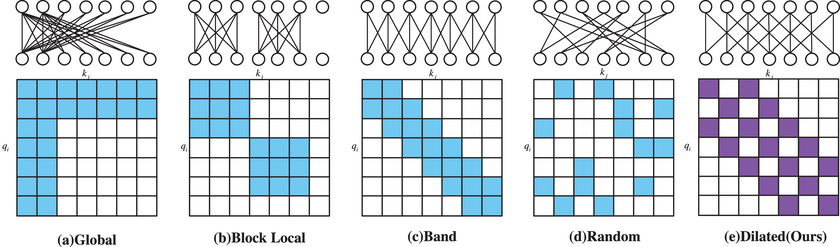
\includegraphics[width=1.0\textwidth]{sparse_attention_patterns.png}
    \captionof{figure}{So sánh các mẫu chú ý thưa (sparse attention). 
    (a) Chú ý toàn cục (Global). 
    (b) Chú ý theo khối cục bộ (Block Local). 
    (c) Chú ý theo dải (Band), hay còn gọi là cửa sổ trượt (Sliding Window). 
    (d) Chú ý ngẫu nhiên (Random). 
    (e) Chú ý giãn cách (Dilated). 
    Các mô hình như Longformer và BigBird thường kết hợp các mẫu này.}
    \label{fig:sparse_attention_patterns}
\end{center}

Hai mô hình tiên phong và tiêu biểu nhất cho trường phái này là Longformer và BigBird.

\subsubsection{Longformer: Kết hợp Cửa sổ trượt và Chú ý Toàn cục}
Longformer (Beltagy et al., 2020) \cite{beltagy2020longformer} đề xuất một mẫu chú ý kết hợp ba thành phần:

\paragraph{1. Chú ý Cửa sổ trượt (Sliding Window Attention)}
\begin{itemize}
    \item \textbf{Cơ chế:} Mỗi token chỉ chú ý đến một cửa sổ có kích thước cố định $w$ gồm các token xung quanh nó (ví dụ: $w/2$ token bên trái và $w/2$ token bên phải).
    \item \textbf{Mục đích:} Nắm bắt ngữ cảnh cục bộ, tương tự như trong các mô hình CNN. Đây là phần lớn các kết nối chú ý trong mô hình.
\end{itemize}

\paragraph{2. Chú ý Cửa sổ trượt Giãn cách (Dilated Sliding Window)}
\begin{itemize}
    \item \textbf{Cơ chế:} Để mở rộng "trường tiếp nhận" (receptive field) mà không tăng chi phí, Longformer sử dụng các cửa sổ trượt có "lỗ" (gaps) ở các lớp khác nhau. Ví dụ, ở một lớp, cửa sổ có thể chú ý đến các token cách nhau 1 vị trí, ở lớp khác, cách nhau 2 vị trí, v.v.
    \item \textbf{Mục đích:} Giúp thông tin từ các token xa hơn có thể được tích hợp vào biểu diễn của một token mà không cần kết nối trực tiếp.
\end{itemize}

\paragraph{3. Chú ý Toàn cục (Global Attention)}
\begin{itemize}
    \item \textbf{Cơ chế:} Một số ít các token được chọn trước được phép chú ý đến \textbf{tất cả} các token khác trong chuỗi, và ngược lại, tất cả các token khác cũng được phép chú ý đến chúng.
    \item \textbf{Mục đích:} Các token toàn cục này hoạt động như một "trung tâm thông tin", tổng hợp và phân phối thông tin trên toàn bộ chuỗi. Các token này thường được chọn một cách đặc biệt, ví dụ như token `[CLS]` trong các tác vụ phân loại.
\end{itemize}

Bằng cách kết hợp các mẫu này, Longformer giảm độ phức tạp tính toán xuống $O(n \cdot w)$, gần như tuyến tính với độ dài chuỗi $n$, cho phép nó xử lý các chuỗi lên tới 4096 token hoặc hơn.

\subsubsection{BigBird: Thêm các Mẫu Chú ý Ngẫu nhiên}
BigBird (Zaheer et al., 2020) \cite{zaheer2020big} có triết lý tương tự Longformer nhưng bổ sung thêm một thành phần:
\begin{itemize}
    \item Nó cũng sử dụng \textbf{Chú ý Cửa sổ trượt} và \textbf{Chú ý Toàn cục}.
    \item Điểm mới lạ là nó thêm vào \textbf{Chú ý Ngẫu nhiên (Random Attention)}. Mỗi token sẽ chú ý đến một số lượng nhỏ $r$ các token được chọn ngẫu nhiên từ toàn bộ chuỗi.
\end{itemize}
Các tác giả đã chứng minh về mặt lý thuyết rằng một mô hình kết hợp ba loại chú ý này (cửa sổ, toàn cục, ngẫu nhiên) có thể xấp xỉ được các thuộc tính của cơ chế chú ý đầy đủ và là một bộ xấp xỉ hàm phổ quát (universal function approximator).

\subsection{Các phương pháp khác: Thoát khỏi Self-Attention Bậc hai}
\label{ssec:other_long_context_methods}

Sparse Attention là một hướng tiếp cận, nhưng không phải là duy nhất. Một hướng đi khác, cấp tiến hơn, là đặt câu hỏi: "Liệu chúng ta có thực sự cần cơ chế chú ý bậc hai không?". Điều này đã dẫn đến sự ra đời của các kiến trúc hoàn toàn mới.
\subsubsection{Cải tiến Mã hóa Vị trí (Positional Encoding)}
Một hướng quan trọng khác để giúp Transformer xử lý ngữ cảnh dài là cải tiến cách nó hiểu về vị trí của token.
\paragraph{ALiBi (Attention with Linear Biases)}
Thay vì thêm mã hóa vị trí vào embedding, ALiBi \cite{press2021train} trực tiếp sửa đổi ma trận điểm chú ý.
\begin{itemize}
    \item \textbf{Cơ chế:} Trước khi qua softmax, điểm chú ý giữa token $i$ và $j$ sẽ bị trừ đi một "án phạt" (penalty) tỷ lệ thuận với khoảng cách của chúng: $\text{score}(i, j) - m \cdot |i - j|$. Trong đó, $m$ là một hệ số học được cho mỗi "đầu" chú ý.
    \item \textbf{Trực giác:} "Các từ càng xa nhau thì càng ít liên quan".
    \item \textbf{Lợi ích:} ALiBi cho thấy khả năng \textbf{ngoại suy (extrapolation)} ấn tượng. Một mô hình được huấn luyện trên ngữ cảnh 2048 token với ALiBi có thể hoạt động tốt trên ngữ cảnh 4096 token hoặc dài hơn mà không cần fine-tuning.
\end{itemize}

\paragraph{RoPE Scaling}
Các mô hình sử dụng Rotary Position Embedding (RoPE) như Llama thường gặp khó khăn khi ngoại suy ra các chuỗi dài hơn độ dài huấn luyện. Các kỹ thuật RoPE Scaling giải quyết vấn đề này.
\begin{itemize}
    \item \textbf{Vấn đề:} RoPE sử dụng các hàm sin/cos với tần số phụ thuộc vào vị trí. Khi vị trí vượt quá giới hạn huấn luyện, các tần số này bắt đầu lặp lại hoặc tạo ra các mẫu không ổn định.
    \item \textbf{Giải pháp (ví dụ:\cite{bloc972023ntkaware}, YaRN \cite{peng2023yarn}):} Các kỹ thuật này sửa đổi "bước sóng" (wavelength) của các hàm sin/cos, về cơ bản là "kéo dãn" không gian vị trí để có thể chứa các chuỗi dài hơn mà không phá vỡ các mối quan hệ tương đối đã học được ở cự ly gần.
\end{itemize}
\subsubsection{Mô hình Trạng thái (State Space Models - SSMs) và Mamba}
Đây là một trong những hướng nghiên cứu thú vị và hứa hẹn nhất gần đây.

\paragraph{Nguồn gốc từ Lý thuyết Điều khiển}
SSMs có nguồn gốc từ lý thuyết điều khiển và xử lý tín hiệu. Chúng được thiết kế để mô hình hóa các hệ thống động liên tục. Ý tưởng cốt lõi là duy trì một \textbf{trạng thái ẩn (state) $h(t)$ nhỏ, có kích thước cố định}, và cập nhật nó một cách liên tục theo thời gian dựa trên đầu vào $x(t)$.
$$ h'(t) = \mathbf{A}h(t) + \mathbf{B}x(t) $$
$$ y(t) = \mathbf{C}h(t) + \mathbf{D}x(t) $$
Trong đó $\mathbf{A, B, C, D}$ là các ma trận tham số.

\paragraph{Thách thức và Giải pháp}
Việc áp dụng trực tiếp SSMs vào học sâu là rất khó khăn về mặt tính toán. Các mô hình như S4 (Structured State Space for Sequence Modeling) \cite{gu2021efficiently} đã giải quyết vấn đề này bằng cách tìm ra một cách hiệu quả để "rời rạc hóa" (discretize) các công thức liên tục này, cho phép chúng được tính toán như một phép tích chập lớn trong quá trình huấn luyện (rất nhanh và song song) và như một RNN trong quá trình suy luận (hiệu quả về bộ nhớ).

\paragraph{Mamba: SSMs có Chọn lọc (Selective SSMs)}
Mamba (Gu \& Dao, 2023) \cite{gu2023mamba} là một bước đột phá lớn dựa trên SSMs. Nó nhận ra rằng một hạn chế của các SSMs trước đó là các ma trận $\mathbf{A, B, C, D}$ là \textbf{cố định}, không phụ thuộc vào đầu vào. Điều này có nghĩa là mô hình không thể thay đổi hành vi của mình dựa trên nội dung cụ thể mà nó đang xử lý.

Mamba đã giải quyết vấn đề này bằng cách làm cho các ma trận $\mathbf{B, C}$ và một tham số bước $\Delta$ \textbf{phụ thuộc vào đầu vào (input-dependent)}.
\paragraph{So sánh SSMs và RNNs truyền thống}
Ở chế độ suy luận, SSM hoạt động tuần tự giống như một RNN. Tuy nhiên, có một sự khác biệt cốt lõi:
\begin{itemize}
    \item \textbf{RNNs (LSTM/GRU):} Việc cập nhật trạng thái ẩn đi qua các cổng phi tuyến phức tạp (sigmoid, tanh). Các cổng này, mặc dù mạnh mẽ, lại làm cho gradient khó chảy ngược qua các chuỗi dài và khó song song hóa trong quá trình huấn luyện.
    \item \textbf{SSMs:} Việc cập nhật trạng thái về bản chất là \textbf{tuyến tính} ($h'(t) = \mathbf{A}h(t) + \dots$). Bản chất tuyến tính này, kết hợp với các ma trận được cấu trúc đặc biệt, cho phép gradient chảy ngược qua các chuỗi rất dài mà không bị triệt tiêu, đồng thời cho phép nó được biến đổi thành một phép tích chập song song hóa được khi huấn luyện.
\end{itemize}
Mamba kế thừa những ưu điểm này và thêm vào đó khả năng chọn lọc thông tin, tạo ra một kiến trúc vừa hiệu quả vừa mạnh mẽ.
\begin{tcolorbox}[
    title=Cơ chế Chọn lọc của Mamba,
    colback=green!5!white, colframe=green!60!black, fonttitle=\bfseries
]
Mamba có khả năng \textbf{chọn lọc} thông tin. Dựa trên token đầu vào hiện tại, nó có thể quyết định:
\begin{enumerate}
    \item \textbf{Tập trung:} Nếu một thông tin quan trọng xuất hiện, nó có thể "mở cổng" để cho thông tin đó đi vào trạng thái ẩn.
    \item \textbf{Lãng quên:} Nếu thông tin hiện tại không còn liên quan, nó có thể "nén" hoặc "quên" đi trạng thái ẩn cũ và đặt lại.
\end{enumerate}
Khả năng chọn lọc này cho phép Mamba nén ngữ cảnh một cách linh hoạt, chỉ giữ lại những gì cần thiết, một khả năng mà các mô hình tích chập hay RNN tuyến tính trước đó không có được.
\end{tcolorbox}

\paragraph{Ưu điểm của Mamba so với Transformer}
\begin{itemize}
    \item \textbf{Độ phức tạp tuyến tính:} Cả huấn luyện và suy luận đều có độ phức tạp $O(n)$, nhanh hơn nhiều so với $O(n^2)$ của Transformer.
    \item \textbf{Suy luận nhanh:} Tốc độ suy luận (sinh từ mới) nhanh hơn Transformer vì nó không cần tính toán lại ma trận chú ý khổng lồ ở mỗi bước.
\end{itemize}
Mamba và các kiến trúc dựa trên SSMs đang nổi lên như một đối thủ cạnh tranh thực sự với Transformer, đặc biệt là trong các kịch bản yêu cầu ngữ cảnh cực dài và hiệu quả tính toán cao.

\subsubsection{Các hướng tiếp cận khác}
Ngoài ra, còn có các hướng tiếp cận khác như:
\begin{itemize}
    \item \textbf{Tích chập có cửa sổ lớn (Large Kernel Convolutions):} Sử dụng các lớp tích chập 1D nhưng với kích thước kernel rất lớn để mô phỏng sự tương tác tầm xa.
    \item \textbf{Phương pháp đệ quy (Recurrence):} Cố gắng đưa trở lại một số dạng của cơ chế RNN để nén thông tin từ các đoạn (chunks) văn bản dài.
\end{itemize}

Việc xử lý ngữ cảnh dài vẫn là một trong những lĩnh vực nghiên cứu năng động nhất, hứa hẹn sẽ mở khóa nhiều khả năng mới cho các mô hình ngôn ngữ trong tương lai.
% % !TEX root = ../main.tex
% File: chapters_part1/chap4_5.tex
% Nội dung cho Chương 4, Phần 5

\section{Lý thuyết về Mixture-of-Experts (MoE)}
\label{sec:mixture_of_experts}

Khi chúng ta nói về việc "tăng quy mô" (scaling up) các mô hình ngôn ngữ, cách tiếp cận thông thường là làm cho các mô hình trở nên "dày đặc" hơn (denser) - tức là tăng số lớp, tăng số chiều ẩn, tăng số đầu chú ý. Tuy nhiên, cách tiếp cận này có một giới hạn: để xử lý mỗi token, \textbf{toàn bộ các tham số của mô hình đều phải được kích hoạt}. Điều này dẫn đến chi phí tính toán cực kỳ lớn ở cả quá trình huấn luyện và suy luận.

Mixture-of-Experts (MoE) \cite{shazeer2017outrageously, fedus2022switch} đưa ra một giải pháp thanh lịch cho vấn đề này, dựa trên một triết lý rất con người:

\begin{tcolorbox}[
    title=Triết lý của Mixture-of-Experts,
    colback=yellow!10!white, colframe=yellow!50!black, fonttitle=\bfseries
]
"Không cần phải huy động toàn bộ bộ não để giải quyết mọi vấn đề. Thay vào đó, hãy có một hội đồng gồm nhiều \textbf{chuyên gia (experts)}, mỗi người chuyên về một lĩnh vực khác nhau. Đối với mỗi vấn đề cụ thể, chỉ cần hỏi ý kiến của một vài chuyên gia phù hợp nhất."
\end{tcolorbox}

Trong bối cảnh của Transformer, MoE cho phép tăng số lượng tham số của mô hình lên rất lớn, nhưng lại giữ cho chi phí tính toán trên mỗi token không đổi hoặc chỉ tăng nhẹ. Đây được gọi là \textbf{tăng quy mô thưa thớt (sparse scaling)}.

\subsection{Kiến trúc và Nguyên lý hoạt động}
\label{ssec:moe_architecture}

Kiến trúc MoE không phải là một mô hình hoàn toàn mới. Thay vào đó, nó là một cách để sửa đổi các khối Transformer hiện có. Cụ thể, trong một khối Transformer tiêu chuẩn, lớp \textbf{Feed-Forward Network (FFN)} được thay thế bằng một \textbf{lớp MoE}.

Một lớp MoE bao gồm hai thành phần chính:
\begin{enumerate}
    \item \textbf{Một tập hợp gồm $N$ mạng FFN độc lập, gọi là các "chuyên gia" (Experts).} Ví dụ, $N$ có thể là 8, 16, hoặc 64. Mỗi chuyên gia này có bộ trọng số riêng.
    \item \textbf{Một mạng cổng (Gating Network) nhỏ.} Đây là một mạng nơ-ron có nhiệm vụ quyết định xem nên gửi mỗi token đến chuyên gia nào.
\end{enumerate}

\begin{center}
    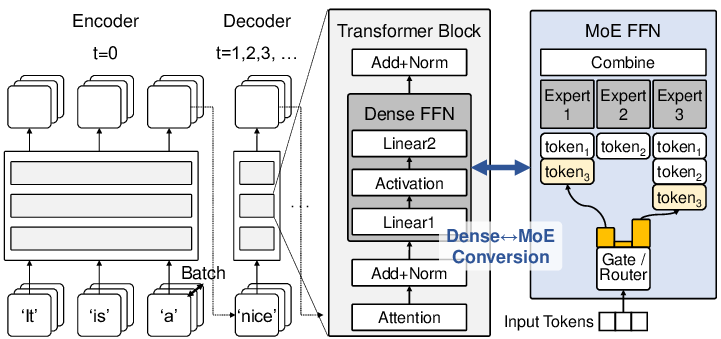
\includegraphics[width=1.0\textwidth]{moe_transformer_block.png}
    \captionof{figure}{So sánh một khối Transformer tiêu chuẩn (trái) và một khối Transformer với lớp MoE (phải). Lớp FFN dày đặc được thay thế bằng một mạng cổng và nhiều chuyên gia FFN thưa thớt.}
    \label{fig:moe_transformer_block}
\end{center}

\subsubsection{Dòng chảy dữ liệu của một token}
Khi một token (được biểu diễn bằng vector $x$) đi vào lớp MoE, quá trình sau sẽ xảy ra:

\paragraph{Bước 1: Định tuyến bởi Mạng cổng (Routing by the Gating Network)}
\begin{itemize}
    \item Token $x$ được đưa vào mạng cổng.
    \item Mạng cổng, thường là một lớp tuyến tính đơn giản, sẽ xuất ra một vector logits có số chiều bằng số chuyên gia ($N$).
    \item Một hàm `softmax` được áp dụng lên vector logits này để tạo ra một phân phối xác suất, $G(x) = (g_1, g_2, \dots, g_N)$, trong đó $g_i$ là "điểm số" hoặc "mức độ tin cậy" mà mạng cổng dành cho chuyên gia thứ $i$.
\end{itemize}

\paragraph{Bước 2: Chọn các Chuyên gia "Top-K"}
\begin{itemize}
    \item Thay vì gửi token đến tất cả các chuyên gia (điều này sẽ làm mất đi tính hiệu quả), hệ thống chỉ chọn ra $k$ chuyên gia có điểm số cao nhất (Top-K routing). Thông thường, $k$ là một số rất nhỏ, ví dụ $k=1$ hoặc $k=2$.
    \item Ví dụ, nếu $k=2$ và chuyên gia thứ 3 và thứ 5 có điểm số cao nhất, thì token này sẽ chỉ được gửi đến hai chuyên gia này. Tất cả các chuyên gia khác sẽ không được kích hoạt cho token này.
\end{itemize}

\paragraph{Bước 3: Xử lý bởi các Chuyên gia}
\begin{itemize}
    \item Token $x$ được đưa qua các mạng FFN của $k$ chuyên gia đã được chọn.
    \item Kết quả đầu ra là $k$ vector: $E_1(x), E_2(x), \dots, E_k(x)$.
\end{itemize}

\paragraph{Bước 4: Tổng hợp có trọng số}
\begin{itemize}
    \item Đầu ra cuối cùng của lớp MoE, $y$, là một tổng có trọng số của đầu ra từ các chuyên gia được chọn. Các trọng số này chính là các điểm số $g_i$ từ mạng cổng đã được chuẩn hóa.
    $$ y = \sum_{i \in \text{TopK}} g_i \cdot E_i(x) $$
\end{itemize}

\subsubsection{Ví dụ: Mixtral 8x7B}
Mô hình Mixtral 8x7B nổi tiếng của Mistral AI là một ví dụ điển hình của MoE.
\begin{itemize}
    \item \textbf{8x7B có nghĩa là gì?} Nó có 8 chuyên gia, mỗi chuyên gia có khoảng 7 tỷ tham số. Tổng số tham số của các lớp MoE là $8 \times 7B = 56B$. Tuy nhiên, đây là số tham số "thưa thớt".
    \item \textbf{Top-2 Routing:} Tại mỗi lớp MoE, mỗi token chỉ được định tuyến đến 2 trong số 8 chuyên gia.
    \item \textbf{Chi phí tính toán:} Do đó, mặc dù tổng số tham số rất lớn, chi phí tính toán để xử lý một token chỉ tương đương với một mô hình dày đặc khoảng $2 \times 7B = 14B$ tham số (cộng với một chi phí nhỏ cho mạng cổng và các lớp khác). Mixtral đạt được chất lượng của một mô hình rất lớn với tốc độ và chi phí của một mô hình nhỏ hơn nhiều.
\end{itemize}
\begin{tcolorbox}[
    title={Các "Chuyên gia" có thực sự chuyên môn hóa không?},
    colback=blue!5!white, colframe=blue!75!black, fonttitle=\bfseries
]
Phép ẩn dụ về "hội đồng chuyên gia" rất hữu ích, nhưng sự chuyên môn hóa của các expert FFN trong thực tế lại trừu tượng hơn nhiều.
\begin{itemize}
    \item \textbf{Không phải là chuyên môn về chủ đề:} Các nghiên cứu đã chỉ ra rằng các expert thường không chuyên môn hóa theo các chủ đề dễ hiểu như "thể thao", "khoa học" hay "lịch sử". Việc định tuyến một token đến expert nào phụ thuộc nhiều vào các đặc trưng trừu tượng của vector biểu diễn của nó.
    \item \textbf{Chuyên môn hóa theo cụm cú pháp/ngữ nghĩa:} Thay vào đó, sự chuyên môn hóa có thể xảy ra ở mức độ thấp hơn. Ví dụ, một số chuyên gia có thể giỏi hơn trong việc xử lý các token là dấu câu, một số khác chuyên về các động từ, một số khác lại tập trung vào các token ở các lớp Transformer cụ thể (ví dụ, các token ở lớp đầu so với lớp cuối).
    \item \textbf{Sự dư thừa có chủ đích:} Có bằng chứng cho thấy các chuyên gia không hoàn toàn độc lập. Thường có sự dư thừa (redundancy) giữa chúng. Điều này có thể là một đặc tính hữu ích, giúp mô hình trở nên mạnh mẽ hơn: nếu một chuyên gia đưa ra kết quả kém, các chuyên gia khác có thể bù đắp.
\end{itemize}
Vì vậy, hãy xem các "chuyên gia" như các \textbf{nhóm tham số (parameter groups)} có thể học được, thay vì các chuyên gia về một lĩnh vực kiến thức cụ thể. Mạng cổng học cách kết hợp các nhóm tham số này một cách tối ưu cho từng token.
\end{tcolorbox}
\subsection{Thách thức trong việc Huấn luyện MoE}
\label{ssec:moe_training_challenges}

Mặc dù rất mạnh mẽ, việc huấn luyện MoE không hề đơn giản và đòi hỏi phải giải quyết một số thách thức đặc thù.

\paragraph{1. Thách thức về sự sụp đổ của việc định tuyến (Routing Collapse)}
Đây là vấn đề lớn nhất của MoE. Nếu không được kiểm soát, mạng cổng sẽ nhanh chóng học được một chiến lược "lười biếng": luôn gửi phần lớn các token đến một hoặc một vài chuyên gia "yêu thích" mà nó cho là tốt nhất.
\begin{itemize}
    \item \textbf{Hậu quả:}
        \begin{enumerate}
            \item \textbf{Lãng phí tham số:} Các chuyên gia khác không nhận được token, do đó không được huấn luyện và trở thành "dead wood". Mô hình MoE khổng lồ sẽ sụp đổ (collapse) thành một mô hình nhỏ hơn nhiều.
            \item \textbf{Mất ổn định huấn luyện:} Gradient sẽ chảy không đều, gây khó khăn cho quá trình tối ưu hóa.
        \end{enumerate}
\end{itemize}

\paragraph{Giải pháp: Hàm Mất mát Cân bằng Tải (Load Balancing Loss)}
Để giải quyết vấn đề này, người ta thêm một \textbf{hàm mất mát phụ trợ (auxiliary loss)} vào hàm mất mát chính của mô hình. Hàm mất mát này được thiết kế để khuyến khích sự phân bổ token đồng đều và thường bao gồm hai thành phần:
\begin{itemize}
    \item \textbf{Một thành phần khuyến khích tầm quan trọng (importance) đồng đều:} Nó phạt nếu tổng các điểm số (logits) mà mạng cổng gán cho mỗi chuyên gia trên toàn bộ một batch là không đồng đều. Điều này đảm bảo mỗi chuyên gia được coi là "quan trọng" như nhau về mặt tổng thể.
    \item \textbf{Một thành phần khuyến khích số lượng token (load) đồng đều:} Nó phạt nếu số lượng token được gửi đến mỗi chuyên gia trong một batch là không đồng đều. Điều này đảm bảo mỗi chuyên gia có "công việc" để làm.
\end{itemize}
Việc cân bằng giữa hàm mất mát chính (ví dụ, cross-entropy) và hàm mất mát phụ trợ này là một trong những khía cạnh nghệ thuật nhất khi huấn luyện các mô hình MoE.

\paragraph{Giải pháp bổ sung: Noisy Top-K Gating}
Một kỹ thuật khác là thêm nhiễu ngẫu nhiên (Gaussian noise) vào logits của mạng cổng trong quá trình huấn luyện.
$$ \text{logits}_{\text{noisy}} = \text{logits}_{\text{original}} + \text{Noise} $$
Nhiễu này buộc mô hình phải "khám phá" (explore) các lựa chọn định tuyến khác nhau thay vì chỉ đi theo con đường quen thuộc, giúp cải thiện sự cân bằng tải một cách tự nhiên.

\paragraph{2. Thách thức về Triển khai và Cơ sở hạ tầng}
\begin{itemize}
    \item \textbf{Bộ nhớ:} Mặc dù chi phí tính toán trên mỗi token thấp, toàn bộ các tham số của tất cả các chuyên gia vẫn phải được tải vào bộ nhớ của GPU, đòi hỏi các hệ thống có bộ nhớ cực lớn.
    \item \textbf{Giao tiếp mạng:} Trong các hệ thống huấn luyện phân tán, các token từ một GPU có thể cần được gửi đến các chuyên gia nằm trên một GPU khác, đòi hỏi băng thông mạng rất cao.
\end{itemize}

\subsection{Tổng kết về MoE}
Mixture-of-Experts là một sự thay đổi mô hình trong cách chúng ta xây dựng các mô hình ngôn ngữ lớn. Nó cho phép chúng ta tách rời \textbf{tổng số tham số} khỏi \textbf{chi phí tính toán trên mỗi token}.

Bằng cách sử dụng các chuyên gia thưa thớt, MoE mở ra một con đường để xây dựng các mô hình có quy mô khổng lồ (hàng nghìn tỷ tham số), có khả năng lưu trữ một lượng kiến thức cực lớn, trong khi vẫn duy trì được tốc độ huấn luyện và suy luận ở mức có thể quản lý được. Đây là một trong những công nghệ nền tảng quan trọng nhất cho thế hệ LLM tiếp theo.

\bigskip
\hrule
\bigskip

\begin{center}
    \textbf{\Large KẾT THÚC CHƯƠNG 4}
\end{center}

\textit{Chương 4 đã là một chuyến đi sâu vào trái tim của NLP hiện đại. Chúng ta đã mổ xẻ kiến trúc Transformer, hiểu được sức mạnh của cơ chế Tự chú ý, và phân loại ba họ mô hình chính -- Encoder-Only, Decoder-Only, và Encoder-Decoder -- đã được sinh ra từ nó. Chúng ta cũng đã khám phá các kỹ thuật tiên tiến cho phép các mô hình này đạt đến quy mô khổng lồ và xử lý ngữ cảnh dài hơn. Về cơ bản, chúng ta đã tìm hiểu cách các "mô hình nền tảng" (foundation models) được xây dựng. Giờ đây, khi đã hiểu rõ cách các mô hình nền tảng khổng lồ này được xây dựng, câu hỏi tiếp theo là: Làm thế nào để chúng ta "thuần hóa" và "chuyên môn hóa" chúng cho các bài toán cụ thể? Chương tiếp theo sẽ tập trung vào các kỹ thuật tinh chỉnh và căn chỉnh, biến những gã khổng lồ đa năng này thành những chuyên gia sắc bén.}
% % !TEX root = ../../main.tex
% File: part2/chapters4/chap4_6.tex

\section{Recipe 6: Trích xuất Thông tin có Cấu trúc từ Văn bản}
\label{sec:recipe_structured_extraction}

\textbf{Mục tiêu:} Trích xuất thông tin từ một đoạn văn bản tự do và trả về dưới dạng một đối tượng JSON có cấu trúc được định nghĩa trước.

\textbf{Thành phần chính:}
\begin{itemize}
    \item \textbf{LLM hỗ trợ Function Calling:} Các mô hình của OpenAI (GPT-3.5/4) hoặc các mô hình mã nguồn mở hỗ trợ chế độ này.
    \item \textbf{Định nghĩa Cấu trúc (Schema):} Một định nghĩa rõ ràng về cấu trúc JSON mong muốn, bao gồm tên các trường, kiểu dữ liệu, và mô tả.
\end{itemize}

\textbf{Các bước thực hiện:}
\begin{enumerate}
    \item \textbf{Định nghĩa "Công cụ":} Mô tả cấu trúc dữ liệu bạn muốn trích xuất dưới dạng một "function signature".
    \item \textbf{Gọi LLM:} Gửi văn bản đầu vào và định nghĩa công cụ đến API của LLM.
    \item \textbf{Phân tích Kết quả:} LLM sẽ trả về một đối tượng JSON tuân thủ theo schema bạn đã định nghĩa.
\end{enumerate}

\textbf{Mã nguồn:}
\begin{example}{Trích xuất Thông tin với OpenAI Function Calling}{ex:function_calling}
    \begin{minted}{python}
    # Bước 1: Cài đặt
    # pip install openai
    import os
    import json
    from openai import OpenAI
    
    # os.environ["OPENAI_API_KEY"] = "sk-..."
    client = OpenAI()
    
    # Bước 2: Định nghĩa "Công cụ" (cấu trúc JSON mong muốn)
    extraction_tool = {
        "type": "function",
        "function": {
            "name": "extract_user_info",
            "description": "Extracts user information from a given text.",
            "parameters": {
                "type": "object",
                "properties": {
                    "name": {
                        "type": "string",
                        "description": "The full name of the user."
                    },
                    "email": {
                        "type": "string",
                        "description": "The email address of the user."
                    },
                    "order_id": {
                        "type": "string",
                        "description": "The ID of the user's order."
                    }
                },
                "required": ["name", "email", "order_id"]
            }
        }
    }
    
    # Văn bản đầu vào
    text_input = """
    Chào bạn, tôi là Trần Văn An, email của tôi là an.tran@example.com.
    Tôi muốn hỏi về tình trạng của đơn hàng #A123-456. Cảm ơn!
    """
    
    # Bước 3: Gọi LLM với công cụ đã định nghĩa
    response = client.chat.completions.create(
        model="gpt-4-turbo",
        messages=[
            {"role": "system", "content": "You are a helpful assistant that extracts structured information."},
            {"role": "user", "content": text_input}
        ],
        tools=[extraction_tool],
        tool_choice={"type": "function", "function": {"name": "extract_user_info"}} # Buộc mô hình phải dùng công cụ này
    )
    
    # Bước 4: Phân tích kết quả
    tool_call = response.choices[0].message.tool_calls[0]
    if tool_call.function.name == "extract_user_info":
        arguments = json.loads(tool_call.function.arguments)
        print("Thông tin đã được trích xuất:")
        print(json.dumps(arguments, indent=2, ensure_ascii=False))
    
    \end{minted}
\end{example}
\textbf{Kết quả mong đợi:}
\begin{minted}{json}
Thông tin đã được trích xuất:
{
  "name": "Trần Văn An",
  "email": "an.tran@example.com",
  "order_id": "A123-456"
}
\end{minted}

\textbf{Lưu ý:} Với các mô hình không hỗ trợ Function Calling, có thể đạt được kết quả tương tự bằng cách sử dụng các thư viện như `Instructor` kết hợp với `Pydantic` để định nghĩa schema và thêm các hướng dẫn chi tiết vào prompt.

\bigskip
\hrule
\bigskip

\begin{center}
    \textbf{\Large KẾT THÚC CHƯƠNG 4}
\end{center}

\textit{Chương 4 đã là một chuyến du hành thực tiễn qua các ứng dụng phổ biến nhất của NLP hiện đại. Bằng cách làm theo các "công thức" chi tiết, bạn đã học được cách kết hợp các thư viện, kiến trúc và kỹ thuật khác nhau để xây dựng các hệ thống hoàn chỉnh. Đây là bước cuối cùng trong việc chuyển hóa kiến thức lý thuyết thành năng lực thực hành. Giờ đây, bạn không chỉ hiểu về NLP, mà còn có đủ công cụ và sự tự tin để bắt đầu xây dựng các giải pháp của riêng mình.}


\clearpage
\thispagestyle{empty}

\begin{center}
    \vspace*{4cm}
    {\Huge \textbf{KẾT THÚC PHẦN 2}} \\[1.5cm]

    \rule{0.8\textwidth}{0.4pt} \\[0.8cm]

    \parbox{0.9\textwidth}{
        \centering
        \textit{
        Phần 2 đã đưa bạn vào một hành trình thực chiến, biến những lý thuyết phức tạp 
        thành các kỹ năng và sản phẩm cụ thể. Từ những bước đầu tiên trong việc 
        xử lý dữ liệu đến việc huấn luyện và triển khai các mô hình ngôn ngữ lớn, 
        bạn đã được trang bị một bộ công cụ toàn diện để giải quyết các bài toán 
        NLP trong thế giới thực. Phần này không chỉ dạy bạn cách sử dụng các thư viện, 
        mà còn rèn luyện một tư duy MLOps bền vững. Với kiến thức từ cả hai phần, 
        bạn đã có đủ hành trang để tự tin bước đi trên con đường của một chuyên gia NLP.
        }
    } \\[1cm]

    \rule{0.8\textwidth}{0.4pt} \\[2cm]
\end{center}

\noindent
\textbf{Tóm lược nội dung Phần 2:}
\begin{itemize}[leftmargin=*]
    \item \textbf{Chương 1 – Quy trình làm việc và Công cụ Xử lý Dữ liệu:} 
    Phác thảo vòng đời dự án NLP tinh gọn, các kỹ thuật thu thập dữ liệu (APIs, Web Scraping), 
    làm sạch và gán nhãn (Pandas, Polars, Label Studio, Snorkel, LLM-based), 
    tăng cường dữ liệu, và quản lý phiên bản với DVC.
    
    \item \textbf{Chương 2 – Huấn luyện và Đánh giá Mô hình:} 
    Làm chủ hệ sinh thái Hugging Face (`transformers`, `datasets`, `accelerate`, `evaluate`), 
    xây dựng các hàm đánh giá thực tế (`compute\_metrics`), theo dõi thí nghiệm 
    (Weights \& Biases, MLflow), và huấn luyện phân tán với DeepSpeed.
    
    \item \textbf{Chương 3 – Tối ưu hóa, Triển khai và Vận hành (MLOps):} 
    Tìm hiểu về Cơ sở dữ liệu Vector, các thư viện tối ưu hóa (`bitsandbytes`, `peft`, ONNX),
    đóng gói và phục vụ mô hình (FastAPI, Docker), các framework chuyên dụng (vLLM, BentoML), 
    và vòng đời MLOps hoàn chỉnh (giám sát, tái huấn luyện).
    
    \item \textbf{Chương 4 – Công thức Xây dựng các Ứng dụng Phổ biến (Recipes):} 
    Hướng dẫn từng bước để xây dựng các ứng dụng thực tế: Tìm kiếm Ngữ nghĩa, 
    Hệ thống RAG, Fine-tuning cho Phân loại và NER, xây dựng Tác tử đơn giản, 
    và Trích xuất Thông tin có Cấu trúc.
\end{itemize}

\bibliographystyle{plain} 
\bibliography{references}

% File: ending.tex
\chapter*{Lời kết}
\addcontentsline{toc}{chapter}{Lời kết} 
\markboth{Lời kết}{} 

\begin{center}
    \vspace*{4cm}
    \rule{0.8\textwidth}{0.4pt} \\[0.8cm]
    \parbox{0.9\textwidth}{
        \centering
        \textit{
        Thế là ta đã đi hết một vòng  Xử lý Ngôn ngữ Tự nhiên. Xin chúc mừng
        }
    } \\[1cm]

    \rule{0.8\textwidth}{0.4pt} \\[2cm]
\end{center}

\noindent
\textbf{Con đường phía trước}

\paragraph{Phần 1}  
Đừng coi “Bách khoa Toàn thư về Lý thuyết” là thứ đọc xong rồi xếp xó. Nó chính là cái nền để bạn dựng mọi mô hình sau này. 
Khi có một paper mới ra với tên nghe như thần chú, quay lại phần này: bạn sẽ thấy bản chất nó vẫn xoay quanh Attention, 
học biểu diễn, và mấy định luật xác suất quen thuộc. Muốn làm pro thật sự thì không chỉ biết xài tool, mà còn phải hiểu vì sao nó chạy được.  

\paragraph{Phần 2}  
“Cẩm nang Thực chiến” đưa công thức cho bạn, nhưng công thức thì sinh ra là để phá. 
Hãy nghịch: đổi mô hình, đổi dữ liệu, phá optimizer, thậm chí làm sai cũng được.  
Mỗi lần máy báo lỗi, hãy coi đó là một mentor thầm lặng. Không giáo trình nào dạy nhanh bằng cách tự fix một đống bug.

\paragraph{Cuối cùng, đừng quên trách nhiệm.}  
NLP không chỉ là code chạy đúng hay loss xuống đẹp. Những mô hình bạn build hôm nay có thể ảnh hưởng đến cách con người giao tiếp, tiếp nhận thông tin.
Thế nên, ngoài chuyện optimize cho nhanh, hãy luôn nghĩ đến bias, fairness, và impact. Làm kỹ sư NLP nên có trách nhiệm đi kèm.

\vfill

\begin{center}
    \parbox{0.9\textwidth}{
        \centering
        {\itshape
        Cảm ơn bạn đã đồng hành tới cuối chặng đường này.  
        Cuốn sách thì đóng lại, nhưng bug thì vẫn còn nhiều, và hành trình học của bạn mới chỉ bắt đầu thôi.  
        Chúc bạn vừa code giỏi, vừa ngủ đủ giấc!
        }
    }
\end{center}

\end{document}
